% Options for packages loaded elsewhere
\PassOptionsToPackage{unicode}{hyperref}
\PassOptionsToPackage{hyphens}{url}
%
\documentclass[
  letterpaper,
]{scrbook}

\usepackage{amsmath,amssymb}
\usepackage{lmodern}
\usepackage{iftex}
\ifPDFTeX
  \usepackage[T1]{fontenc}
  \usepackage[utf8]{inputenc}
  \usepackage{textcomp} % provide euro and other symbols
\else % if luatex or xetex
  \usepackage{unicode-math}
  \defaultfontfeatures{Scale=MatchLowercase}
  \defaultfontfeatures[\rmfamily]{Ligatures=TeX,Scale=1}
\fi
% Use upquote if available, for straight quotes in verbatim environments
\IfFileExists{upquote.sty}{\usepackage{upquote}}{}
\IfFileExists{microtype.sty}{% use microtype if available
  \usepackage[]{microtype}
  \UseMicrotypeSet[protrusion]{basicmath} % disable protrusion for tt fonts
}{}
\makeatletter
\@ifundefined{KOMAClassName}{% if non-KOMA class
  \IfFileExists{parskip.sty}{%
    \usepackage{parskip}
  }{% else
    \setlength{\parindent}{0pt}
    \setlength{\parskip}{6pt plus 2pt minus 1pt}}
}{% if KOMA class
  \KOMAoptions{parskip=half}}
\makeatother
\usepackage{xcolor}
\usepackage[left=1in,marginparwidth=2.0666666666667in,textwidth=4.1333333333333in,marginparsep=0.3in]{geometry}
\usepackage[normalem]{ulem}
\setlength{\emergencystretch}{3em} % prevent overfull lines
\setcounter{secnumdepth}{5}
% Make \paragraph and \subparagraph free-standing
\ifx\paragraph\undefined\else
  \let\oldparagraph\paragraph
  \renewcommand{\paragraph}[1]{\oldparagraph{#1}\mbox{}}
\fi
\ifx\subparagraph\undefined\else
  \let\oldsubparagraph\subparagraph
  \renewcommand{\subparagraph}[1]{\oldsubparagraph{#1}\mbox{}}
\fi

\usepackage{color}
\usepackage{fancyvrb}
\newcommand{\VerbBar}{|}
\newcommand{\VERB}{\Verb[commandchars=\\\{\}]}
\DefineVerbatimEnvironment{Highlighting}{Verbatim}{commandchars=\\\{\}}
% Add ',fontsize=\small' for more characters per line
\usepackage{framed}
\definecolor{shadecolor}{RGB}{241,243,245}
\newenvironment{Shaded}{\begin{snugshade}}{\end{snugshade}}
\newcommand{\AlertTok}[1]{\textcolor[rgb]{0.68,0.00,0.00}{#1}}
\newcommand{\AnnotationTok}[1]{\textcolor[rgb]{0.37,0.37,0.37}{#1}}
\newcommand{\AttributeTok}[1]{\textcolor[rgb]{0.40,0.45,0.13}{#1}}
\newcommand{\BaseNTok}[1]{\textcolor[rgb]{0.68,0.00,0.00}{#1}}
\newcommand{\BuiltInTok}[1]{\textcolor[rgb]{0.00,0.23,0.31}{#1}}
\newcommand{\CharTok}[1]{\textcolor[rgb]{0.13,0.47,0.30}{#1}}
\newcommand{\CommentTok}[1]{\textcolor[rgb]{0.37,0.37,0.37}{#1}}
\newcommand{\CommentVarTok}[1]{\textcolor[rgb]{0.37,0.37,0.37}{\textit{#1}}}
\newcommand{\ConstantTok}[1]{\textcolor[rgb]{0.56,0.35,0.01}{#1}}
\newcommand{\ControlFlowTok}[1]{\textcolor[rgb]{0.00,0.23,0.31}{#1}}
\newcommand{\DataTypeTok}[1]{\textcolor[rgb]{0.68,0.00,0.00}{#1}}
\newcommand{\DecValTok}[1]{\textcolor[rgb]{0.68,0.00,0.00}{#1}}
\newcommand{\DocumentationTok}[1]{\textcolor[rgb]{0.37,0.37,0.37}{\textit{#1}}}
\newcommand{\ErrorTok}[1]{\textcolor[rgb]{0.68,0.00,0.00}{#1}}
\newcommand{\ExtensionTok}[1]{\textcolor[rgb]{0.00,0.23,0.31}{#1}}
\newcommand{\FloatTok}[1]{\textcolor[rgb]{0.68,0.00,0.00}{#1}}
\newcommand{\FunctionTok}[1]{\textcolor[rgb]{0.28,0.35,0.67}{#1}}
\newcommand{\ImportTok}[1]{\textcolor[rgb]{0.00,0.46,0.62}{#1}}
\newcommand{\InformationTok}[1]{\textcolor[rgb]{0.37,0.37,0.37}{#1}}
\newcommand{\KeywordTok}[1]{\textcolor[rgb]{0.00,0.23,0.31}{#1}}
\newcommand{\NormalTok}[1]{\textcolor[rgb]{0.00,0.23,0.31}{#1}}
\newcommand{\OperatorTok}[1]{\textcolor[rgb]{0.37,0.37,0.37}{#1}}
\newcommand{\OtherTok}[1]{\textcolor[rgb]{0.00,0.23,0.31}{#1}}
\newcommand{\PreprocessorTok}[1]{\textcolor[rgb]{0.68,0.00,0.00}{#1}}
\newcommand{\RegionMarkerTok}[1]{\textcolor[rgb]{0.00,0.23,0.31}{#1}}
\newcommand{\SpecialCharTok}[1]{\textcolor[rgb]{0.37,0.37,0.37}{#1}}
\newcommand{\SpecialStringTok}[1]{\textcolor[rgb]{0.13,0.47,0.30}{#1}}
\newcommand{\StringTok}[1]{\textcolor[rgb]{0.13,0.47,0.30}{#1}}
\newcommand{\VariableTok}[1]{\textcolor[rgb]{0.07,0.07,0.07}{#1}}
\newcommand{\VerbatimStringTok}[1]{\textcolor[rgb]{0.13,0.47,0.30}{#1}}
\newcommand{\WarningTok}[1]{\textcolor[rgb]{0.37,0.37,0.37}{\textit{#1}}}

\providecommand{\tightlist}{%
  \setlength{\itemsep}{0pt}\setlength{\parskip}{0pt}}\usepackage{longtable,booktabs,array}
\usepackage{calc} % for calculating minipage widths
% Correct order of tables after \paragraph or \subparagraph
\usepackage{etoolbox}
\makeatletter
\patchcmd\longtable{\par}{\if@noskipsec\mbox{}\fi\par}{}{}
\makeatother
% Allow footnotes in longtable head/foot
\IfFileExists{footnotehyper.sty}{\usepackage{footnotehyper}}{\usepackage{footnote}}
\makesavenoteenv{longtable}
\usepackage{graphicx}
\makeatletter
\def\maxwidth{\ifdim\Gin@nat@width>\linewidth\linewidth\else\Gin@nat@width\fi}
\def\maxheight{\ifdim\Gin@nat@height>\textheight\textheight\else\Gin@nat@height\fi}
\makeatother
% Scale images if necessary, so that they will not overflow the page
% margins by default, and it is still possible to overwrite the defaults
% using explicit options in \includegraphics[width, height, ...]{}
\setkeys{Gin}{width=\maxwidth,height=\maxheight,keepaspectratio}
% Set default figure placement to htbp
\makeatletter
\def\fps@figure{htbp}
\makeatother
\newlength{\cslhangindent}
\setlength{\cslhangindent}{1.5em}
\newlength{\csllabelwidth}
\setlength{\csllabelwidth}{3em}
\newlength{\cslentryspacingunit} % times entry-spacing
\setlength{\cslentryspacingunit}{\parskip}
\newenvironment{CSLReferences}[2] % #1 hanging-ident, #2 entry spacing
 {% don't indent paragraphs
  \setlength{\parindent}{0pt}
  % turn on hanging indent if param 1 is 1
  \ifodd #1
  \let\oldpar\par
  \def\par{\hangindent=\cslhangindent\oldpar}
  \fi
  % set entry spacing
  \setlength{\parskip}{#2\cslentryspacingunit}
 }%
 {}
\usepackage{calc}
\newcommand{\CSLBlock}[1]{#1\hfill\break}
\newcommand{\CSLLeftMargin}[1]{\parbox[t]{\csllabelwidth}{#1}}
\newcommand{\CSLRightInline}[1]{\parbox[t]{\linewidth - \csllabelwidth}{#1}\break}
\newcommand{\CSLIndent}[1]{\hspace{\cslhangindent}#1}

\usepackage{booktabs}
\usepackage{longtable}
\usepackage{array}
\usepackage{multirow}
\usepackage{wrapfig}
\usepackage{float}
\usepackage{colortbl}
\usepackage{pdflscape}
\usepackage{tabu}
\usepackage{threeparttable}
\usepackage{threeparttablex}
\usepackage[normalem]{ulem}
\usepackage{makecell}
\usepackage{xcolor}
\makeatletter
\@ifpackageloaded{tcolorbox}{}{\usepackage[many]{tcolorbox}}
\@ifpackageloaded{fontawesome5}{}{\usepackage{fontawesome5}}
\definecolor{quarto-callout-color}{HTML}{909090}
\definecolor{quarto-callout-note-color}{HTML}{0758E5}
\definecolor{quarto-callout-important-color}{HTML}{CC1914}
\definecolor{quarto-callout-warning-color}{HTML}{EB9113}
\definecolor{quarto-callout-tip-color}{HTML}{00A047}
\definecolor{quarto-callout-caution-color}{HTML}{FC5300}
\definecolor{quarto-callout-color-frame}{HTML}{acacac}
\definecolor{quarto-callout-note-color-frame}{HTML}{4582ec}
\definecolor{quarto-callout-important-color-frame}{HTML}{d9534f}
\definecolor{quarto-callout-warning-color-frame}{HTML}{f0ad4e}
\definecolor{quarto-callout-tip-color-frame}{HTML}{02b875}
\definecolor{quarto-callout-caution-color-frame}{HTML}{fd7e14}
\makeatother
\makeatletter
\makeatother
\makeatletter
\@ifpackageloaded{bookmark}{}{\usepackage{bookmark}}
\makeatother
\makeatletter
\@ifpackageloaded{caption}{}{\usepackage{caption}}
\AtBeginDocument{%
\ifdefined\contentsname
  \renewcommand*\contentsname{Inhaltsverzeichnis}
\else
  \newcommand\contentsname{Inhaltsverzeichnis}
\fi
\ifdefined\listfigurename
  \renewcommand*\listfigurename{Abbildungsverzeichnis}
\else
  \newcommand\listfigurename{Abbildungsverzeichnis}
\fi
\ifdefined\listtablename
  \renewcommand*\listtablename{Tabellenverzeichnis}
\else
  \newcommand\listtablename{Tabellenverzeichnis}
\fi
\ifdefined\figurename
  \renewcommand*\figurename{Abbildung}
\else
  \newcommand\figurename{Abbildung}
\fi
\ifdefined\tablename
  \renewcommand*\tablename{Tabelle}
\else
  \newcommand\tablename{Tabelle}
\fi
}
\@ifpackageloaded{float}{}{\usepackage{float}}
\floatstyle{ruled}
\@ifundefined{c@chapter}{\newfloat{codelisting}{h}{lop}}{\newfloat{codelisting}{h}{lop}[chapter]}
\floatname{codelisting}{Listing}
\newcommand*\listoflistings{\listof{codelisting}{Listingverzeichnis}}
\makeatother
\makeatletter
\@ifpackageloaded{caption}{}{\usepackage{caption}}
\@ifpackageloaded{subcaption}{}{\usepackage{subcaption}}
\makeatother
\makeatletter
\@ifpackageloaded{tcolorbox}{}{\usepackage[many]{tcolorbox}}
\makeatother
\makeatletter
\@ifundefined{shadecolor}{\definecolor{shadecolor}{rgb}{.97, .97, .97}}
\makeatother
\makeatletter
\@ifpackageloaded{sidenotes}{}{\usepackage{sidenotes}}
\@ifpackageloaded{marginnote}{}{\usepackage{marginnote}}
\makeatother
\makeatletter
\makeatother
\ifLuaTeX
\usepackage[bidi=basic]{babel}
\else
\usepackage[bidi=default]{babel}
\fi
\babelprovide[main,import]{ngerman}
% get rid of language-specific shorthands (see #6817):
\let\LanguageShortHands\languageshorthands
\def\languageshorthands#1{}
\ifLuaTeX
  \usepackage{selnolig}  % disable illegal ligatures
\fi
\IfFileExists{bookmark.sty}{\usepackage{bookmark}}{\usepackage{hyperref}}
\IfFileExists{xurl.sty}{\usepackage{xurl}}{} % add URL line breaks if available
\urlstyle{same} % disable monospaced font for URLs
\hypersetup{
  pdftitle={Skript Bio Data Science},
  pdfauthor={Prof.~Dr.~Jochen Kruppa},
  pdflang={de},
  hidelinks,
  pdfcreator={LaTeX via pandoc}}

\title{Skript Bio Data Science}
\author{Prof.~Dr.~Jochen Kruppa}
\date{13. September 2022}

\begin{document}
\frontmatter
\maketitle
\ifdefined\Shaded\renewenvironment{Shaded}{\begin{tcolorbox}[interior hidden, borderline west={3pt}{0pt}{shadecolor}, boxrule=0pt, enhanced, frame hidden, sharp corners, breakable]}{\end{tcolorbox}}\fi

\renewcommand*\contentsname{Inhaltsverzeichnis}
{
\setcounter{tocdepth}{2}
\tableofcontents
}
\mainmatter
\bookmarksetup{startatroot}

\hypertarget{willkommen}{%
\chapter*{Willkommen}\label{willkommen}}
\addcontentsline{toc}{chapter}{Willkommen}

Auf den folgenden Seiten wirst du eine Menge über Statistik oder Data
Science lernen. Du musst dafür nicht eine meiner Veranstaltungen
besuchen. Gerne kannst du hier und dort einmal schauen, ob etwas für
dich dabei ist. Das Skript wird fortlaufend von mir ergänzt. Neben dem
Skript gibt es auch noch die erklärenden YouTube Videos. Ich freue mich,
dass du Lust hast hier etwas zu lernen\ldots{} oder aber du \emph{musst}
-- da bald eine Klausur ansteht. Wie auch immer -- schau dich einfach
mal um. Im Anhang findest du auch einen kleinen Leitfaden für das
Schreiben einer Abschlussarbeit. Vielleicht hilft dir die Anleitung ja
beim Schreiben.

\begin{tcolorbox}[enhanced jigsaw, coltitle=black, titlerule=0mm, bottomrule=.15mm, opacityback=0, opacitybacktitle=0.6, leftrule=.75mm, title=\textcolor{quarto-callout-caution-color}{\faFire}\hspace{0.5em}{Gesammelte Klausurfragen Bio Data Science}, toprule=.15mm, bottomtitle=1mm, toptitle=1mm, left=2mm, breakable, arc=.35mm, colback=white, rightrule=.15mm, colbacktitle=quarto-callout-caution-color!10!white, colframe=quarto-callout-caution-color-frame]
Du findest die
\href{https://github.com/jkruppa/teaching/tree/main/Klausur}{gesammelten
Klausurfragen auf GitHub}. Die Klausurfragen zu den einzelnen
Vorlesungen in einem Modul werden in den entsprechenden Übungen
besprochen. Bitte komme in die Übungen.
\end{tcolorbox}

\hypertarget{lernen}{%
\section*{Lernen\ldots{}}\label{lernen}}
\addcontentsline{toc}{section}{Lernen\ldots{}}

Du liest hier gerade das Skript für
\protect\hyperlink{sec-vorlesungen-hs}{meine Vorlesungen} an der
Hochschule Osnabrück an der Fakultät Agrarwissenschaften und
Landschaftsarchitektur (AuL). Wie immer Leben kannst du auf verschiedene
Arten und Weisen den Stoff, den ich vermitteln will, lernen. Daher gibt
es noch zwei andere Möglichkeiten. Zum einen Lernen auf YouTube, mit
meinen Lernvideos oder du schaust dir das Material auf GitHub an. Auf
GitHub habe ich auch Informationen, die du vielleicht brauchen kannst.
Ebenso findest du im Kapitel~\ref{sec-literatur} noch andere
Literaturempfehlungen.

\hypertarget{auf-youtube}{%
\subsection*{\ldots{} auf YouTube}\label{auf-youtube}}
\addcontentsline{toc}{subsection}{\ldots{} auf YouTube}

\begin{figure}

{\centering 
\includegraphics[width=3.125in,height=\textheight]{./images/youtube.png}

}

\end{figure}

Wenn du möchtest kannst du auf YouTube unter
\url{https://www.youtube.com/c/JochenKruppa} noch einige Lehrvideos als
Ergänzung schauen. In den Videos wiederhole ich Inhalte und du kannst
auf Pause drücken um nochmal Programmierschritte nachverfolgen zu
können.

\hypertarget{auf-github}{%
\subsection*{\ldots{} auf GitHub}\label{auf-github}}
\addcontentsline{toc}{subsection}{\ldots{} auf GitHub}

\begin{figure}

{\centering 
\includegraphics[width=3.125in,height=\textheight]{./images/github.png}

}

\end{figure}

Alle Materialien von mir findest du immer auf GitHub unter
\url{https://github.com/jkruppa/teaching}. Selbst wenn du nicht mehr in
einem meiner Kurse bist, kannst du so auf die Lehrinhalte immer nochmal
zugreifen und die aktuellen Versionen haben. Auf GitHub liegt auch immer
eine semesteraktuelle Version der
\href{https://github.com/jkruppa/teaching/tree/main/Klausur}{gesammelten
Klausurfragen} für meine Module.

\hypertarget{sec-contact-mail}{%
\section*{Kontakt}\label{sec-contact-mail}}
\addcontentsline{toc}{section}{Kontakt}

Wie erreichst du mich? Am einfachsten über die gute, alte E-Mail. Bitte
bachte, dass gerade kurz vor den Prüfungen ich mehr E-Mails kriege.
Leider kann es dann einen Tick dauern.

\begin{figure}

{\centering 
\includegraphics[width=2.08333in,height=\textheight]{./images/mail.png}

}

\end{figure}

Einfach an
\href{mailto:j.kruppa@hs-osnabrueck.de}{\nolinkurl{j.kruppa@hs-osnabrueck.de}}
schreiben. Du findest hier auch eine kurze Formulierungshilfe. Einfach
auf den Ausklapppfeil klicken.

\textbf{Bitte gib immer in deiner E-Mail dein Modul - was du belegst -
mit an.} Pro Semester unterrichte ich immer \emph{drei} sehr ähnlich
klingende Module. Daher schau nochmal
\protect\hyperlink{sec-vorlesungen-hs}{hier in der Liste}, wenn du
unsicher bist.

\begin{tcolorbox}[enhanced jigsaw, coltitle=black, titlerule=0mm, bottomrule=.15mm, opacityback=0, opacitybacktitle=0.6, leftrule=.75mm, title=\textcolor{quarto-callout-tip-color}{\faLightbulb}\hspace{0.5em}{E-Mailvorlage mit beispielhafter Anrede}, toprule=.15mm, bottomtitle=1mm, toptitle=1mm, left=2mm, breakable, arc=.35mm, colback=white, rightrule=.15mm, colbacktitle=quarto-callout-tip-color!10!white, colframe=quarto-callout-tip-color-frame]
Hallo Herr Kruppa,

\ldots{} ich belege gerade Ihr Modul \texttt{Modulname} und hätte eine
Bitte/Frage/Anregung\ldots{}

\ldots{} ich benötige Hilfe bei der Planung/Auswertung meiner
Bachelorarbeit\ldots{}

Mit freundlichen Grüßen

M. Muster
\end{tcolorbox}

\bookmarksetup{startatroot}

\hypertarget{organisation}{%
\chapter{Organisation}\label{organisation}}

\emph{Version vom September 14, 2022 um 08:44:28}

Den Teil kannst du hier überspringen, wenn es dich nicht so richtig
interessiert, was ich alles an Vorlesungen an der Hochschule Osnabrück
anbiete. Wenn es dir um \emph{statistische} Inhalte geht, dann gehe
einfach weiter in die nächsten Kapitel. In diesem Kapitel geht es
nochmal Orientierung über meine Vorlesungen zu geben, wenn dich noch
mehr als nur der Pflichtkurs interessiert.

\hypertarget{statistische-beratung}{%
\section{Statistische Beratung}\label{statistische-beratung}}

Neben der klassischen Vorlesung biete ich auch Termine für die
statistische Beratung von Abschlussarbeiten sowie Projekten an. Dieses
Angebot gilt es für alle Mitglieder der Hochschule Osnabrück. Primär für
Fakultät Agrarwissenschaften und Landschaftsarchitektur (AuL), aber
ntürlich auch für alle anderen Fakultäten. Dafür musst du mir einfach
nur eine \protect\hyperlink{sec-contact-mail}{E-Mail schreiben} und dann
erhälst du einen Termin innerhalb der nächsten zwei Wochen.

Die Beratung ist grundsätzlich anonym und vertraulich. Wenn du willst
kannst du gerne noch dein:e Betreuer:in mitbringen. Das ist aber keine
Voraussetzung oder Notwendigkeit. Meistens finden mehrere Besprechungen
statt, wir versuchen aber natürlich zusammen zügig dein Problem zu
lösen. Ziel ist der Beratung ist es dich in die Lage zu versetzen
selbstständig deine Analyse zu rechnen.

\hypertarget{sec-r-tutorium}{%
\section{R Tutorium}\label{sec-r-tutorium}}

Zusätzlich zu der statistischen Beratung bieten wir auch ein R Tutorium
für alle Mitglieder der Fakultät Agrarwissenschaften und
Landschaftsarchitektur (AuL) an. Theoretisch können auch hier andere
Mitglieder der anderen Faklutäten vorbeischauen, der Ort ist aber
aktuell ein Raum auf dem Gelände in Haste. Die aktuellen Termine findest
du in Tabelle~\ref{tbl-r-tutorium}.

Im R Tutorium besprechen wir aktuelle Themen der Teilnehmer:innen. Meist
sind dies aktuelle Fragen zu den Bachelorarbeiten. Auch wenn du kein
dringendes Problem hast, kannst du gerne kommen und dir die
Fragestellungen anhören. Meistens ist es auch interessant mal die
Fragestellungen der anderen Studierenden sich anzuhören oder aber schon
mal zu Üben ein anderes Experiment zu verstehen.

Bitte beachte folgende Hinweise zu den Terminen.

\begin{tcolorbox}[enhanced jigsaw, coltitle=black, titlerule=0mm, bottomrule=.15mm, opacityback=0, opacitybacktitle=0.6, leftrule=.75mm, title=\textcolor{quarto-callout-note-color}{\faInfo}\hspace{0.5em}{Hinweise zu dem R Tutorium}, toprule=.15mm, bottomtitle=1mm, toptitle=1mm, left=2mm, breakable, arc=.35mm, colback=white, rightrule=.15mm, colbacktitle=quarto-callout-note-color!10!white, colframe=quarto-callout-note-color-frame]
Das R Tutorium findet \textbf{nicht} im Prüfungszeitraum der Fakultät
Agrarwissenschaften und Landschaftsarchitektur (AuL) statt.

Das R Tutorium findet \textbf{nicht} im \emph{Februar} und \emph{März}
statt.

Das R Tutorium findet \textbf{nicht} im \emph{August} und
\emph{September} statt.
\end{tcolorbox}

\hypertarget{tbl-r-tutorium}{}
\begin{longtable}[]{@{}llll@{}}
\caption{\label{tbl-r-tutorium}Aktuelle Termine des R Tutoriums im
Semester}\tabularnewline
\toprule()
Termin & Uhrzeit & Raum & Anmerkung \\
\midrule()
\endfirsthead
\toprule()
Termin & Uhrzeit & Raum & Anmerkung \\
\midrule()
\endhead
\emph{nächste} & \emph{Termine} & \emph{ab} & \emph{Oktober 2022} \\
\bottomrule()
\end{longtable}

\hypertarget{sec-vorlesungen-hs}{%
\section{Vorlesungen an der Hochschule
Osnabrück}\label{sec-vorlesungen-hs}}

Von mir angebotene Vorlesungen werden an der Hochschule Osnabrück an der
Fakultät Agrarwissenschaften und Landschaftsarchitektur (AuL) in ILIAS
verwaltet. Alle notwendigen Informationen und Materialien sind auf ILIAS
unter \url{https://lms.hs-osnabrueck.de/} zu finden. Wenn du in dem Kurs
nicht angemeldet bist, dann kontaktiere mich bitte
\protect\hyperlink{sec-contact-mail}{per Mail}. Auch die Kommunikation
erfolgt von meiner Seite aus über ILIAS.

{\marginnote{\begin{footnotesize}Auf ILIAS findest du alle aktuellen
Kursinformationen und erhälst auch die Mails, wenn Änderungen im
Kursablauf stattfinden.\end{footnotesize}}}

Wenn du nicht in der Fakultät Agrarwissenschaften und
Landschaftsarchitektur (AuL) studierst oder aber in einem Studiengang,
der meine Module nicht anbietet, steht es dir natürlich frei, sich in
meine Vorlesungen zu setzten. Du findest in Tabelle~\ref{tbl-angebot}
eine Übersicht der angebotenen Module und auch die inhaltliche Ordnung
nach Lernstufe. Bitte informiere dich in deinem Studierendensekretariat
über die Modalitäten zur Prüfungsteilnahme.

Eine inhaltliche Übersicht findet sich auf dem
\href{https://docs.google.com/spreadsheets/d/1WCTnJnofz5OrGZth6LKyPGQvQUUw31t7OfnAE6yz-ww/edit?usp=sharing}{Google
Spreadsheet}. Die Planung ist aktuell (Stand Herbst/Winter 2022) noch
nicht abgeschlossen. Im Zweifel einfach bei mir einmal
\protect\hyperlink{sec-contact-mail}{per Mail} anfragen.

\begin{figure*}

\hypertarget{tbl-angebot}{}
\begin{longtable}[]{@{}
  >{\raggedright\arraybackslash}p{(\columnwidth - 8\tabcolsep) * \real{0.0206}}
  >{\raggedright\arraybackslash}p{(\columnwidth - 8\tabcolsep) * \real{0.2588}}
  >{\raggedright\arraybackslash}p{(\columnwidth - 8\tabcolsep) * \real{0.2588}}
  >{\raggedright\arraybackslash}p{(\columnwidth - 8\tabcolsep) * \real{0.2794}}
  >{\raggedright\arraybackslash}p{(\columnwidth - 8\tabcolsep) * \real{0.1824}}@{}}
\caption{\label{tbl-angebot}Angebotene Statistik Module an der Fakultät
Agrarwissenschaften und Landschaftsarchitektur (AuL). Die Stufe gibt das
Lernniveau an.}\tabularnewline
\toprule()
\begin{minipage}[b]{\linewidth}\raggedright
Stufe
\end{minipage} & \begin{minipage}[b]{\linewidth}\raggedright
\textbf{Landwirtschaft; Angewandte Pflanzenbiologie -- Gartenbau,
Pflanzentechnologie}
\end{minipage} & \begin{minipage}[b]{\linewidth}\raggedright
\textbf{Wirtschafts- ingenieurwesen Agrar / Lebensmittel}
\end{minipage} & \begin{minipage}[b]{\linewidth}\raggedright
\textbf{Bioverfahrenstechnik in Agrar- und Lebensmittelwirtschaft}
\end{minipage} & \begin{minipage}[b]{\linewidth}\raggedright
\textbf{Angewandte Nutztier- und Pflanzenwissenschaften}
\end{minipage} \\
\midrule()
\endfirsthead
\toprule()
\begin{minipage}[b]{\linewidth}\raggedright
Stufe
\end{minipage} & \begin{minipage}[b]{\linewidth}\raggedright
\textbf{Landwirtschaft; Angewandte Pflanzenbiologie -- Gartenbau,
Pflanzentechnologie}
\end{minipage} & \begin{minipage}[b]{\linewidth}\raggedright
\textbf{Wirtschafts- ingenieurwesen Agrar / Lebensmittel}
\end{minipage} & \begin{minipage}[b]{\linewidth}\raggedright
\textbf{Bioverfahrenstechnik in Agrar- und Lebensmittelwirtschaft}
\end{minipage} & \begin{minipage}[b]{\linewidth}\raggedright
\textbf{Angewandte Nutztier- und Pflanzenwissenschaften}
\end{minipage} \\
\midrule()
\endhead
\textbf{1} &
\href{https://www.hs-osnabrueck.de/module/44b0266/}{Mathematik und
Statistik} &
\href{https://www.hs-osnabrueck.de/module/44b0568/}{Statistik} &
\href{https://www.hs-osnabrueck.de/module/44b0567/}{Angewandte Statistik
für Bioverfahrenstechnik} & \\
\textbf{2} &
\href{https://www.hs-osnabrueck.de/module/44b0400/}{Angewandte Statistik
und Versuchswesen} &
\href{https://www.hs-osnabrueck.de/module/44b0400/}{Angewandte Statistik
und Versuchswesen} & & \\
\textbf{3} &
\href{https://www.hs-osnabrueck.de/module/44b0390/}{Spezielle Statistik
und Versuchswesen} & & &
\href{https://www.hs-osnabrueck.de/module/44m0161/}{Biostatistik} \\
\bottomrule()
\end{longtable}

\end{figure*}

\bookmarksetup{startatroot}

\hypertarget{sec-literatur}{%
\chapter{Literatur}\label{sec-literatur}}

\emph{Version vom September 14, 2022 um 08:44:32}

Was ist gute Literatur? Immer schwer zu beurteilen. Im Folgenden liste
ich einige Literaturquellen auf. Zum einen basiert eine Menge von dem R
Code auf Wickham (2016) zum Anderen möchtest du dich vielleicht nochmal
rechts oder links weiter bilden. Du musst aber nicht um die Klausur
bestehen zu können. Siehe es eher als ein Angebot.

\begin{tcolorbox}[enhanced jigsaw, coltitle=black, titlerule=0mm, bottomrule=.15mm, opacityback=0, opacitybacktitle=0.6, leftrule=.75mm, title=\textcolor{quarto-callout-note-color}{\faInfo}\hspace{0.5em}{Die Frage nach der Klausur\ldots{}}, toprule=.15mm, bottomtitle=1mm, toptitle=1mm, left=2mm, breakable, arc=.35mm, colback=white, rightrule=.15mm, colbacktitle=quarto-callout-note-color!10!white, colframe=quarto-callout-note-color-frame]
Und daher hier nochmal gleich zu Anfang, es ist nicht notwendig mehr als
das Skript durchzuarbeiten und bei den Übungen zu sein um die Klausur zu
bestehen. Für deine Bachelorarbeit wirst du aber Programmieren in R
können müssen.
\end{tcolorbox}

Neben diesem Modul musst du vermutlich noch andere Module belegen.
Deshalb hier eine Auswahl Literatur, die dir helfen mag. Zum einen ist
die Literatur anders geschrieben und zum anderen sind dort andere
Inhalte.

\hypertarget{parametrische-statistik}{%
\section{Parametrische Statistik}\label{parametrische-statistik}}

\begin{figure}

{\centering 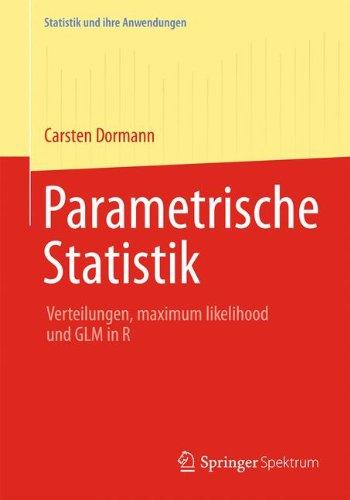
\includegraphics[width=2.08333in,height=\textheight]{./images/dormann.jpg}

}

\end{figure}

Dormann (2013) liefert ein tolles deutsches Buch für die Vertiefung in
die Statistik. Insbesondere wenn du wissenschaftlich Arbeiten willst
weit über die Bachelorarbeit hinaus. Dormann baut in seinem Buch eine
hervorragende Grundlage auf. Das Buch ist an der Hochschule Osnabrück
kostenlos
\href{https://link.springer.com/book/10.1007/978-3-662-54684-0}{über den
Link} zu erhalten.

\hypertarget{experimental-methods-in-agriculture}{%
\section{Experimental methods in
agriculture}\label{experimental-methods-in-agriculture}}

\begin{figure}

{\centering 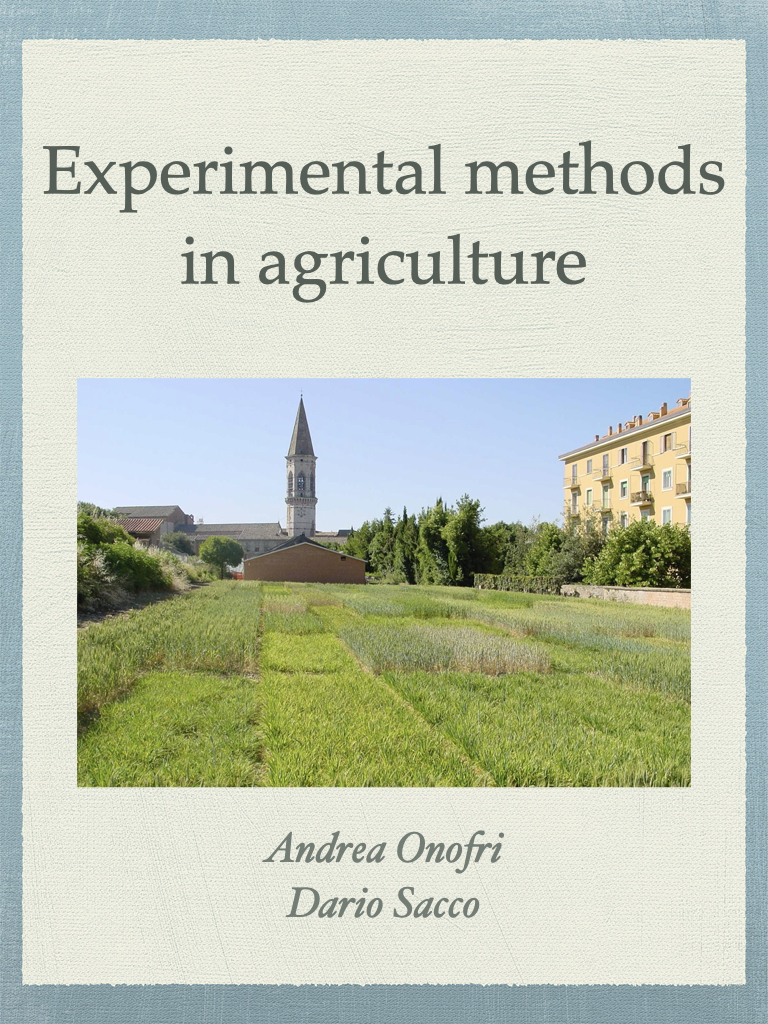
\includegraphics[width=2.08333in,height=\textheight]{./images/cover_stat_for_biology.jpeg}

}

\end{figure}

Onofri und Sacco (2021) haben das Buch
\href{https://www.statforbiology.com/_statbookeng/}{Experimental methods
in agriculture} geschrieben. Wir werden auf dieses englische Buch ab und
zu mal verweisen. Insbesondere der Einleitungstext zur Wissenschaft und
dem Design von Experiementen ist immer wieder lesenswert. Spätere Teile
des Buches sind etwas mathematischer und nicht für den Einstieg
unbedingt geeignet. Aber schaue es dir selber an.

\hypertarget{r-for-data-science}{%
\section{R for Data Science}\label{r-for-data-science}}

\begin{figure}

{\centering 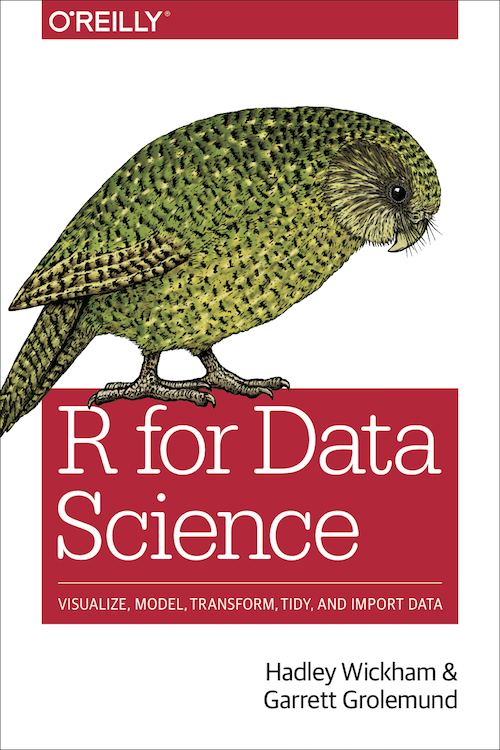
\includegraphics[width=2.08333in,height=\textheight]{./images/hadley.png}

}

\end{figure}

Wickham (2016) ist die Grundlage für die R Programmierung. Das Material
von Wickahm findet sich kostenlos online unter
\url{https://r4ds.had.co.nz/} und \url{https://www.tidyverse.org/}. Wir
werden uns hauptsächlich mit R wie es Wickham lehrt beschäftigen. Somit
ist Wickham unsere Grundlage für R.

\hypertarget{practical-statistics-for-data-scientists}{%
\section{Practical Statistics for Data
Scientists}\label{practical-statistics-for-data-scientists}}

\begin{figure}

{\centering 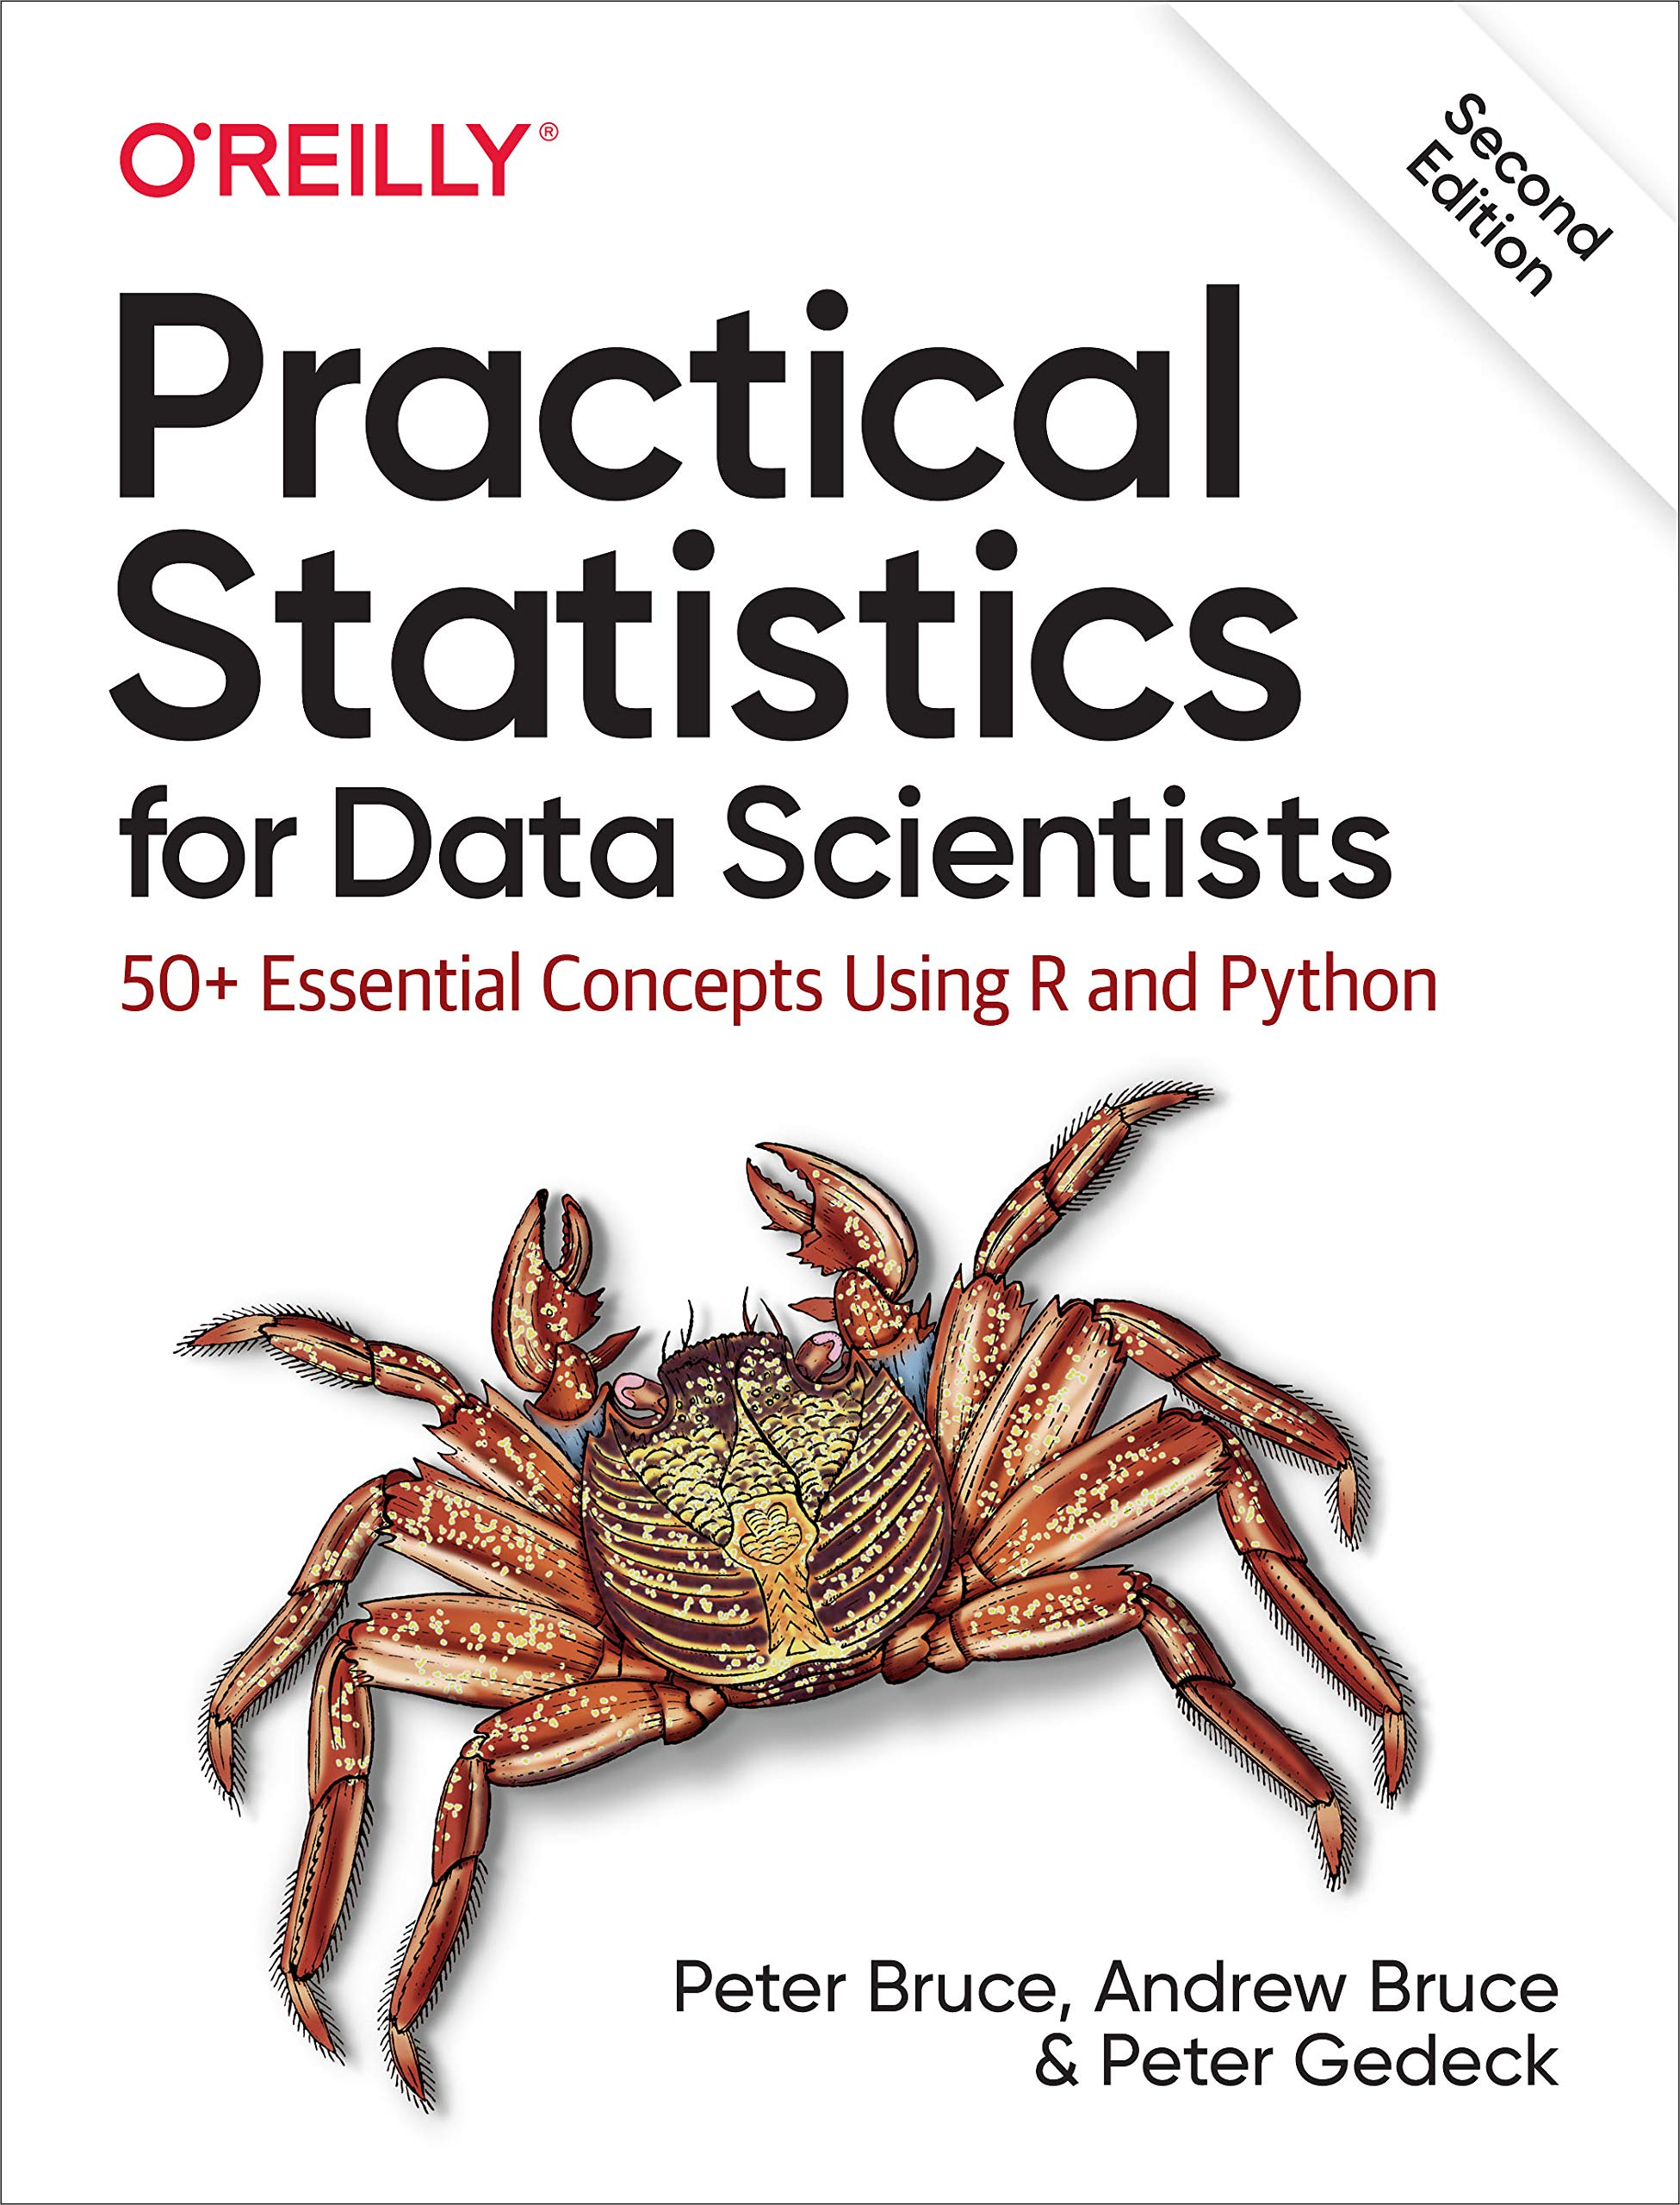
\includegraphics[width=2.08333in,height=\textheight]{./images/practical.jpg}

}

\end{figure}

Bruce (2020) schreibt ein Buch für den Anwender. Ohne Vorkenntnisse ist
das Buch vermutlich etwas schwer zu lesen. Dafür bietet das Buch aber
\emph{nach} einem Statistikkurs sehr gute Anknüpfungspunkte Richtung
maschinelles Lernen und somit der Klassifikation. Das Buch ist auch hier
in der
\href{https://ebookcentral.proquest.com/lib/hs-osnabrueck/detail.action?docID=6173908}{englischen
Version} und hier in der
\href{http://www.content-select.com/index.php?id=bib_view\&ean=9783960104674}{deutschen
Version} zu erhalten. \emph{Beide Links benötigen den Zugang über die
Hochschule Osnabrück}.

\hypertarget{data-science-for-agriculture-in-r}{%
\section{Data Science for Agriculture in
R}\label{data-science-for-agriculture-in-r}}

\begin{figure}

{\centering 
\includegraphics{./images/dsfair.png}

}

\end{figure}

Schmidt liefert auf der Webseite
\url{https://schmidtpaul.github.io/DSFAIR/index.html} eine tolle
Sammlung an experimentellen Designs bzw. Versuchsanlagen samt der
Auswertung in R. Ohne Vorkenntnisse schwer zu verstehen. Sollte aber
nach einem Kurs Statistik dann möglich sein. Gerne hier auch mich
fragen, dann können wir gemeinsam das passende Design raussuchen und
besprechen.

\hypertarget{odds-ends}{%
\section{Odds \& Ends}\label{odds-ends}}

\begin{figure}

{\centering 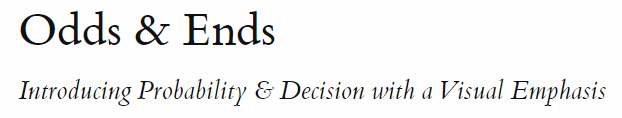
\includegraphics{./images/odds_and_ends.PNG}

}

\end{figure}

Am Ende dann noch eine Mathebuch von Weisberg zu finden unter
\url{https://jonathanweisberg.org/vip/}. Eigentlich eher ein Buch über
Wahrscheinlichkeiten und wenn ein Buch am Ende stehen muss, dann ist es
dieses Buch. Ich finde es sehr spannend zu lesen, aber das ist dann
vermutlich \emph{special intrest}.

\hypertarget{referenzen}{%
\section*{Referenzen}\label{referenzen}}
\addcontentsline{toc}{section}{Referenzen}

\bookmarksetup{startatroot}

\hypertarget{einfuxfchrung}{%
\chapter{Einführung}\label{einfuxfchrung}}

\emph{Version vom September 14, 2022 um 08:44:40}

In diesem Kapitel nenne ich die wichtigsten Lernziele, die nach dem
Lesen des Skriptes im Rahmen deiner Lehrveranstaltung von dir erreicht
worden sein sollten. Je nach besuchten Kurs kann natürlich nicht
\emph{alles} geschafft worden sein. Viele Kapitel haben noch eine
Abschnitt in dem du mehr über die Klausur erfährst. So sehe diese
Übersicht als Einführung für das was später an Lehrinhalten kommt. Wenn
du die Lernziele hier verstehst, dann hast du eine gute und solide
Grundlage in Statistik und Bio Data Science. Damit solltest du dann auch
gut durch die Anfänge deiner Bachelorarbeit kommen.

\hypertarget{ein-wort-der-warnung}{%
\section*{Ein Wort der Warnung\ldots{}}\label{ein-wort-der-warnung}}
\addcontentsline{toc}{section}{Ein Wort der Warnung\ldots{}}

Wenn du dieses Bild eines niedergeschlagenen \emph{Engels der Statistik}
siehst\ldots{}

\begin{figure}

{\centering 
\includegraphics[width=0.3\textwidth,height=\textheight]{./images/angel_01.png}

}

\end{figure}

\ldots{} dann bedeutet der niedergeschlagene Engel der Statistik:

\begin{enumerate}
\def\labelenumi{\arabic{enumi})}
\tightlist
\item
  Wir opfern Genauigkeit für Anwendbarkeit. Ja, manchmal ist es eben
  statstisch nicht richtig was hier steht, aber aus Gründen der
  Anwendung fahren wir mal über den Engel drüber. \emph{Schade}.
\item
  Wir sind hier Anfänger und Anwender. Später kannst du noch tiefer ins
  Detail gehen. Hier wollen wir die Grundlagen lernen. Das hat dann
  einen Preis an \emph{Richtigkeit}.
\item
  Wir wollen fertig werden. Durch geschicktes Manövrieren können wir an
  einen Punkt kommen, wo kein statistischer Test mehr passt. Das wollen
  wir nicht. Deshalb zahlen wir hier auch einen Preis. Passt aber.
\end{enumerate}

Deshalb konzentrieren wir uns auf einige wichtige Lernziele, die wir
jetzt einmal nacheinander durchgehen.

\hypertarget{lernziel-1-eine-explorative-datananalyse-durchfuxfchren}{%
\section{Lernziel 1: Eine explorative Datananalyse
durchführen}\label{lernziel-1-eine-explorative-datananalyse-durchfuxfchren}}

Gleich zu Beginn R Code zu zeigen und eine entsprechende Abbildung ist
vielleicht ungewöhnlich, aber wir wollen zu dieser
Abbildung~\ref{fig-boxplot-preface} hin. In
Abbildung~\ref{fig-boxplot-preface} siehst du einen Boxplot. Und wie wir
aus den Daten \texttt{flea\_dog\_cat.xlsx} einen Boxplot erstellen, das
soll uns in den nächsten Kapitel beschäftigen. Dafür müssen wir nämlich
eine Menge in dem Codeblock verstehen und dann auch Anwenden können. Und
natürlich lernen was eigentlich ein Boxplot ist und was in einem Boxplot
eigentlich dargestellt ist.

\begin{figure}

{\centering 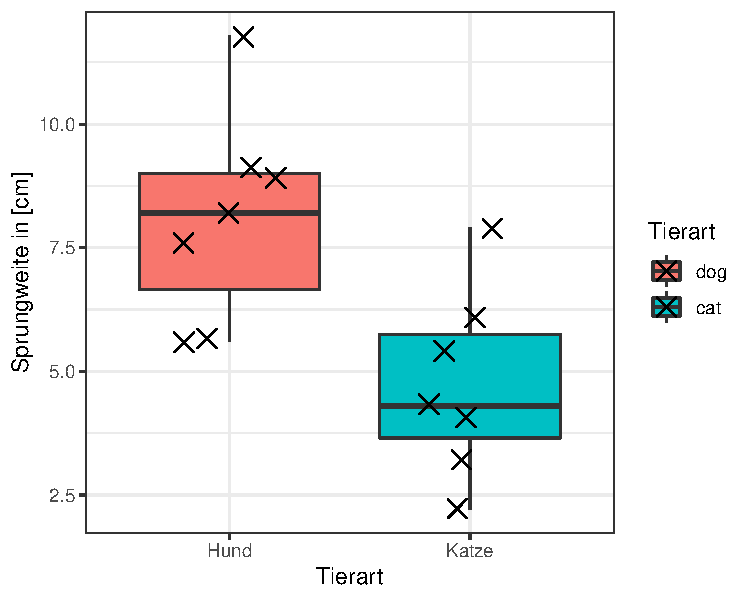
\includegraphics{./preface_files/figure-pdf/fig-boxplot-preface-1.pdf}

}

\caption{\label{fig-boxplot-preface}Boxplot der Sprungweiten {[}cm{]}
von Hunden und Katzen.}

\end{figure}

Hier ist der Codeblock der in R die Abbildung~\ref{fig-boxplot-preface}
erstellt.

\begin{Shaded}
\begin{Highlighting}[]
\DocumentationTok{\#\# Einlesen von Daten aus Excel}
\NormalTok{data\_tbl }\OtherTok{\textless{}{-}} \FunctionTok{read\_excel}\NormalTok{(}\StringTok{"data/flea\_dog\_cat.xlsx"}\NormalTok{)}

\DocumentationTok{\#\# Umformen der \textless{}chr\textgreater{} Spalte in einen Factor \textless{}fct\textgreater{}}
\NormalTok{data\_tbl }\OtherTok{\textless{}{-}}\NormalTok{ data\_tbl }\SpecialCharTok{\%\textgreater{}\%} 
  \FunctionTok{mutate}\NormalTok{(}\AttributeTok{animal =} \FunctionTok{as\_factor}\NormalTok{(animal))}

\DocumentationTok{\#\# Auswählen der wichtigen Spalten für den Boxplot}
\NormalTok{data\_tbl }\OtherTok{\textless{}{-}}\NormalTok{ data\_tbl }\SpecialCharTok{\%\textgreater{}\%} 
  \FunctionTok{select}\NormalTok{(animal, jump\_length) }

\DocumentationTok{\#\# Generieren des Boxplots in ggplot()}
\FunctionTok{ggplot}\NormalTok{(data\_tbl, }\FunctionTok{aes}\NormalTok{(}\AttributeTok{x =}\NormalTok{ animal, }\AttributeTok{y =}\NormalTok{ jump\_length, }
                     \AttributeTok{fill =}\NormalTok{ animal)) }\SpecialCharTok{+}
  \FunctionTok{geom\_boxplot}\NormalTok{() }\SpecialCharTok{+}
  \FunctionTok{geom\_jitter}\NormalTok{() }\SpecialCharTok{+}
  \FunctionTok{labs}\NormalTok{(}\AttributeTok{x =} \StringTok{"Tierart"}\NormalTok{, }\AttributeTok{y =} \StringTok{"Sprungweite in [cm]"}\NormalTok{, }
       \AttributeTok{fill =} \StringTok{"Tierart"}\NormalTok{) }\SpecialCharTok{+}
  \FunctionTok{scale\_x\_discrete}\NormalTok{(}\AttributeTok{labels =} \FunctionTok{c}\NormalTok{(}\StringTok{"Hund"}\NormalTok{, }\StringTok{"Katze"}\NormalTok{)) }\SpecialCharTok{+}
  \FunctionTok{theme\_bw}\NormalTok{()}
\end{Highlighting}
\end{Shaded}

Wir müssen nun folgende Dinge lernen um den Codeblock zu verstehen:

\begin{itemize}
\tightlist
\item
  Wir müssen das Datenbeispiel verstehen. Was sind das eigentlich für
  Daten, die wir da abbilden? Was sind überhaupt Daten im Sinne der
  Statistik bzw. für R.
\item
  Wir müssen den R Code verstehen. Von einzelnen wichtigen Operatoren
  wie \texttt{-\textgreater{}} und
  \texttt{\%\textbackslash{}\textgreater{}\%} zu dem den Unterschieden
  von Worten und Objekten.
\item
  Wie kriegen wir Daten aus Excel in R hinein? Wir können die Daten ja
  nicht einfach in R eintragen sondern haben die Daten ja meist in einer
  (Excel) Datei wie \texttt{flea\_dog\_cat.xlsx}.
\item
  Was ist eigentlich ein Boxplot und welche statistischen Maßzahlen
  werden hier eigentlich abgebildet?
\item
  Wie funktioniert eigentlich die Funktionalen \texttt{ggplot()} mit der
  wir den Boxplot erstellt haben?
\end{itemize}

All diese Fragen und weitere Fragen, die sich diesen Fragen anschließen,
wollen wir uns in den nächsten Kapitel anschauen. Leider kann ich hier
nur \emph{linear} schreiben. Deshalb musst du eventuell mal ein Kapitel
wiederholen oder etwas quer lesen. Du kannst dir ja auch nicht immer
alles auf einmal merken.

\hypertarget{lernziel-2-rstudio-und-r}{%
\section{Lernziel 2: RStudio und R}\label{lernziel-2-rstudio-und-r}}

\begin{tcolorbox}[enhanced jigsaw, coltitle=black, titlerule=0mm, bottomrule=.15mm, opacityback=0, opacitybacktitle=0.6, leftrule=.75mm, title=\textcolor{quarto-callout-tip-color}{\faLightbulb}\hspace{0.5em}{Was ist eigentlich RStudio und woher kriege ich das?}, toprule=.15mm, bottomtitle=1mm, toptitle=1mm, left=2mm, breakable, arc=.35mm, colback=white, rightrule=.15mm, colbacktitle=quarto-callout-tip-color!10!white, colframe=quarto-callout-tip-color-frame]
Du findest auf YouTube \href{https://youtu.be/krF7TJVb-UA}{Einführung in
R - Teil 01 - Installation von RStudio und R} als Video. Ich gehe in dem
Video einmal alle wichtigen Schritte durch und so kannst du dir Rstudio
und R installieren.
\end{tcolorbox}

Um Data Science durchführen zu können musst du etwas Programmieren
können. Wir programmieren in R und nutzen die Software um Abbildungen zu
erstellen und Analysen zu rechnen.

Wir arbeiten in R und nutzen dafür das RStudio. Führe einfach folgende
Schritte aus um erst R zu installieren und dann das RStudio.

\begin{enumerate}
\def\labelenumi{\arabic{enumi}.}
\tightlist
\item
  R installieren unter \url{https://cran.rstudio.com/}
\item
  RStudio installieren unter
  \url{https://www.rstudio.com/products/rstudio/download/\#download}
\end{enumerate}

Bitte die Reihenfolge beachten. Beide Schritte kannst du dir auch
nochmals im Video anschauen oder aber du kommst in das R Tutorium was
regelmäßig an der Hochschule Osnabrück von mir angeboten wird. Die
Termine findest du im Kapitel~\ref{sec-r-tutorium}.

\hypertarget{lernziel-3-falsifikationsprinzip}{%
\section{Lernziel 3:
Falsifikationsprinzip}\label{lernziel-3-falsifikationsprinzip}}

\begin{tcolorbox}[enhanced jigsaw, coltitle=black, titlerule=0mm, bottomrule=.15mm, opacityback=0, opacitybacktitle=0.6, leftrule=.75mm, title=\textcolor{quarto-callout-tip-color}{\faLightbulb}\hspace{0.5em}{Grundlagen der Wissenschaft und Falsifikationsprinzip}, toprule=.15mm, bottomtitle=1mm, toptitle=1mm, left=2mm, breakable, arc=.35mm, colback=white, rightrule=.15mm, colbacktitle=quarto-callout-tip-color!10!white, colframe=quarto-callout-tip-color-frame]
Du findest auf YouTube \href{https://youtu.be/h45ftLNsspM}{Grundlagen
der Wissenschaft und Falsifikationsprinzip} als Video Reihe.
\end{tcolorbox}

Wie funktioniert ein \emph{statistischer} Versuch? Ich könnte auch
wissenschaftliches Experiment schreiben, aber ein wissenschaftliches
Experiment ist sehr abstrakt. Wir wollen ja einen Versuch durchführen
und danach - ja was eigentlich? Was wollen wir nach dem Versuch haben?
Meistens eine neue Erkenntnis. Um diese Erkenntnis zu validieren oder
aber abzusichern nutzen wir Statistik. Dazu musst du noch wissen, dass
wir eine spezielle Form der Statistik nutzen: die \emph{frequentistische
Statistik}.

{\marginnote{\begin{footnotesize}Eine \textbf{biologische Wiederholung}
beinhaltet ein neues Tier, Pflanze oder Mensch. Eine \textbf{technische}
Wiederholung ist die gleiche Messung an dem gleichen Tier, Pflanze oder
Mensch.\end{footnotesize}}}

{\marginnote{\begin{footnotesize}Wir nennen das \textbf{Outcome} auch
\textbf{Endpunkt}, \textbf{Response} oder kurz
\(y\).\end{footnotesize}}}

Die \emph{frequentistische Statistik} basiert - wie der Name andeutet -
auf Wiederholungen in einem Versuch. Daher der Name frequentistisch.
Also eine Frequenz von Beobachtungen. Ist ein wenig gewollt, aber daran
gewöhnen wir uns schon mal. Konkret, ein Experiment welches wir
frequentistisch Auswerten wollen besteht immer aus biologischen
Wiederholungen. Wir müssen also ein Experiment planen in dem wir
wiederholt ein Outcome an vielen Tieren, Pflanzen oder Menschen messen.
Auf das Outcome gehen wir noch später ein. Im Weiteren konzentrieren wir
uns hier auf die \emph{parametrische} Statistik. Die parametrische
Statistik beschäftigt sich mit Parametern von Verteilungen.

\begin{tcolorbox}[enhanced jigsaw, coltitle=black, titlerule=0mm, bottomrule=.15mm, opacityback=0, opacitybacktitle=0.6, leftrule=.75mm, title=\textcolor{quarto-callout-note-color}{\faInfo}\hspace{0.5em}{Wie gehen wir nun vor, wenn wir ein Experiment durchführen wollen?}, toprule=.15mm, bottomtitle=1mm, toptitle=1mm, left=2mm, breakable, arc=.35mm, colback=white, rightrule=.15mm, colbacktitle=quarto-callout-note-color!10!white, colframe=quarto-callout-note-color-frame]

\begin{enumerate}
\def\labelenumi{\arabic{enumi})}
\tightlist
\item
  Wir müssen auf jeden Fall wiederholt ein Outcome an verschiedenen
  Tieren, Pflanzen oder Menschen messen.
\item
  Wir überlegen uns aus welcher Verteilungsfamilie unser Outcome stammt,
  damit wir dann die entsprechende Verfahren zur Analyse nehmen können.
\end{enumerate}

\end{tcolorbox}

Wenn wir nun ein Experiment durchführen dann erheben wir einmalig Daten
\(D_1\). Wir könnten das Experiment wiederholen und erneut Daten \(D_2\)
erheben. Wir können das Experiment \(j\)-mal wiederholen und haben dann
Daten von \(D_1,..., D_j\). Dennoch werden wir nie \emph{alle} Daten
erheben können, die mit einem Experiment verbunden sind.

{\marginnote{\begin{footnotesize}\textbf{Strukturgleichkeit} erreichen
wir durch \textbf{Randomisierung}.\end{footnotesize}}}

Nehmen wir das Beispiel, dass wir die Sprungweite von Hunde- und
Katzenflöhen vergleichen wollen. Wir können nicht \emph{alle} Hunde- und
Katzenflöhe messen. Wir können nur eine Stichprobe an Daten \(D_1\)
erheben. Über diese Daten \(D_1\) können wir dann später durch
statistische Algorithmen eine Aussage treffen. Wichtig ist hier sich zu
merken, dass wir eine Grundgesamtheit haben aus der wir eine Stichprobe
ziehen. Wir müssen darauf achten, dass die Stichprobe
\emph{repräsentativ} ist und damit \emph{strukturgleich} zur
Grundgesamtheit ist. Die Strukturgleichkeit erreichen wir durch
Randomisierung. Wir veranschaulichen diesen Zusammenhang in
Abbildung~\ref{fig-grundgesamtheit-schema}. Ein Rückschluß von der
Stichprobe ist nur möglich, wenn die Stichprobe die Grundgesamtheit
repräsentiert. Auch eine Randomisierung mag dieses Ziel nicht immer
erreichen. Im Beispiel der Hundeflöhe könnte wir eine Art an Flöhen
übersehen und diese Flohart nicht mit in die Stichprobe aufnehmen. Ein
Rückschluß auf diese Flohart wäre dann mit unserem Experiment nicht
möglich.

\begin{figure}

{\centering 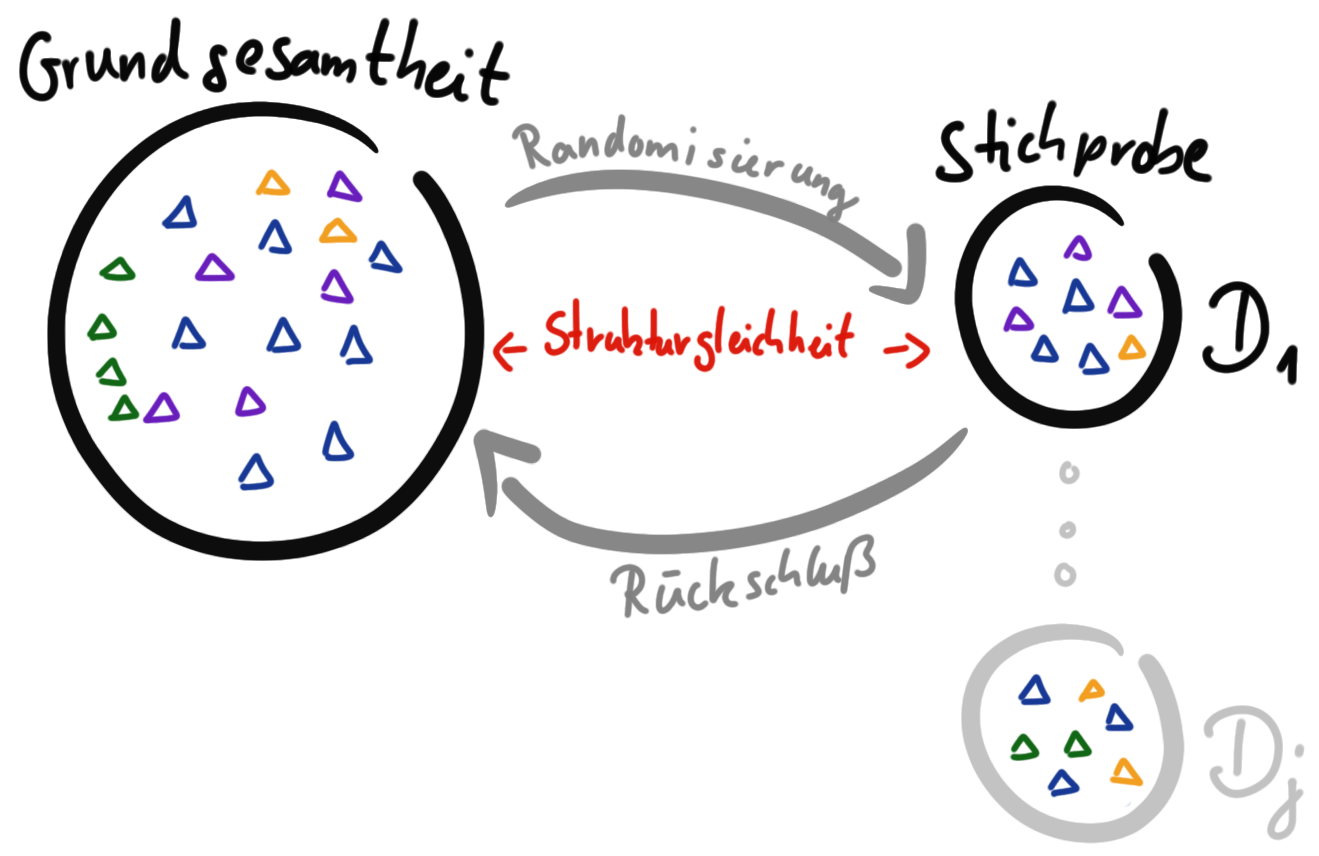
\includegraphics[width=0.8\textwidth,height=\textheight]{./images/preface-grundgesamtheit.png}

}

\caption{\label{fig-grundgesamtheit-schema}Abbildung über die
Grundgesamtheit und die Stichprobe(n) \(D_1\) bis \(D_j\). Durch
Randomisierung wird Sturkturgleichheit erreicht, die dann einen
Rückschluß von der Stichprobe auf die Grundgesamtheit erlaubt. Jede
Stichprobe ist anders und nicht jede Randomisierung ist erfolgreich was
die Strukturgleicheit betrifft.}

\end{figure}

Tabelle~\ref{tbl-grundgesamtheit-stichprobe} zeigt nochmal die
Zusammenfassung von der Grundgesamtheit un der Stichprobe im Vergleich.
Wichtig ist zu merken, dass wir mit unserem kleinen Experiment Daten
\(D\) generieren mit denen wir einen Rückschluß und somit eine
Verallgemeinerung erreichen wollen.

\hypertarget{tbl-grundgesamtheit-stichprobe}{}
\begin{longtable}[]{@{}
  >{\raggedright\arraybackslash}p{(\columnwidth - 2\tabcolsep) * \real{0.5221}}
  >{\raggedright\arraybackslash}p{(\columnwidth - 2\tabcolsep) * \real{0.4779}}@{}}
\caption{\label{tbl-grundgesamtheit-stichprobe}Vergleich von
Grundgesamtheit und Stichprobe.}\tabularnewline
\toprule()
\begin{minipage}[b]{\linewidth}\raggedright
Grundgesamtheit
\end{minipage} & \begin{minipage}[b]{\linewidth}\raggedright
Stichprobe
\end{minipage} \\
\midrule()
\endfirsthead
\toprule()
\begin{minipage}[b]{\linewidth}\raggedright
Grundgesamtheit
\end{minipage} & \begin{minipage}[b]{\linewidth}\raggedright
Stichprobe
\end{minipage} \\
\midrule()
\endhead
\ldots{} \(n\) ist riesig bis unfassbar. & \ldots{} \(n\) von \(D\) ist
klein. \\
\ldots{} der Mittelwert wird mit \(\mu_y\) beschrieben. & \ldots{} der
Mittelwert wird mit \(\bar{y}\) beschrieben. \\
\ldots{} die Varianz wird mit \(\sigma^2\) beschrieben. & \ldots{} die
Varianz wird mit \(s^2\) beschrieben. \\
\ldots{} die Standardabweichung wird mit \(\sigma\) beschrieben. &
\ldots{} die Standardabweichung wird mit \(s\) beschrieben. \\
\bottomrule()
\end{longtable}

\part{Datenbeispiele}

\emph{Version vom September 14, 2022 um 08:44:50}

Wir brauchen am Anfang erstmal ein simples Beispiel. Konkrete Zahlen mit
denen wir arbeiten können und Grundlagen aufbauen können. Was liegt da
näher als sich einmal am Kopf zu kratzen und zu fragen, was juckt den
da? Genau! Flöhe. Wir schauen uns einmal Flöhe auf Hunden und Katzen an.
Daran können wir viel über Zahlen und Buchstaben in der Statistik und
dann im Programmieren lernen.

\begin{tcolorbox}[enhanced jigsaw, coltitle=black, titlerule=0mm, bottomrule=.15mm, opacityback=0, opacitybacktitle=0.6, leftrule=.75mm, title=\textcolor{quarto-callout-note-color}{\faInfo}\hspace{0.5em}{Zahlen, Buchstaben und Wörter}, toprule=.15mm, bottomtitle=1mm, toptitle=1mm, left=2mm, breakable, arc=.35mm, colback=white, rightrule=.15mm, colbacktitle=quarto-callout-note-color!10!white, colframe=quarto-callout-note-color-frame]
Mir ist bewusst, dass du die Unterschiede kennst. Nur leider ist eine
Zahl nicht nur eine Zahl und ein Wort nicht immer ein Wort. Das hat mit
der eingeschränkten Kommunikationsfähigkeit von Computerprogrammen zu
tun. R braucht da deine Mithilfe und dein \emph{neues} Verständnis von
Buchstaben und Zahlen. Eben wie ein Computer denkt.
\end{tcolorbox}

\hypertarget{von-fluxf6hen-und-hunden}{%
\section*{Von Flöhen und Hunden}\label{von-fluxf6hen-und-hunden}}
\addcontentsline{toc}{section}{Von Flöhen und Hunden}

In unserem ersten Beispiel in Kapitel~\ref{sec-example-1} geht es darum
einmal ein Gefühl für Daten zu kriegen. Also was sind diese Zahlen und
Buchstaben eigentlich? Wie sind Daten aufgebaut und wie musst du Daten
bauen, so dass wir auch mit den Daten arbeiten können? Wir schauen uns
dafür einmal Flöhe auf Hunden an und fragen uns welche Typen von Zahlen
können wir erheben?

\hypertarget{von-fluxf6hen-hunden-und-katzen}{%
\section*{Von Flöhen, Hunden und
Katzen}\label{von-fluxf6hen-hunden-und-katzen}}
\addcontentsline{toc}{section}{Von Flöhen, Hunden und Katzen}

In unserem zweiten Beispiel in Kapitel~\ref{sec-example-2} erweitern wir
unserer erstes Beispiel um die Katzen. Das heist, dass eigentlich alles
gleich bleibt. Wir schauen usn \emph{zusätlich} noch als zweite Gruppe
die Katzen an. Nun können wir die Frage stellen, unterscheiden sich
Flöhe auf Hunden und Katzen gegeben von gemessenen Eigenschaften?

\hypertarget{von-fluxf6hen-auf-tieren}{%
\section*{Von Flöhen auf Tieren}\label{von-fluxf6hen-auf-tieren}}
\addcontentsline{toc}{section}{Von Flöhen auf Tieren}

In unserem dritten Beispiel in Kapitel~\ref{sec-example-3} erweitern wir
das Beispiel um den Fuchs mit einem weiteren Tier. Dadurch haben wir
nicht mehr einen Faktor mit zwei Leveln vorliegen sondern einen mit drei
Leveln. Die Fragestrellung erweitert sich jetzt auf einen
\emph{multiplen} Gruppenvergleich. Wir vergleichen nicht mehr nur noch
zwei Gruppen miteinander sondern drei.

\hypertarget{von-fluxf6hen-auf-tieren-in-habitaten}{%
\section*{Von Flöhen auf Tieren in
Habitaten}\label{von-fluxf6hen-auf-tieren-in-habitaten}}
\addcontentsline{toc}{section}{Von Flöhen auf Tieren in Habitaten}

In unserem vierten Beispiel in Kapitel~\ref{sec-example-4} schauen wir
uns zusätzlich zu dem dritten Beispiel noch verschiedene Habitate (eng.
\emph{site}) an. Wir haben nämlich die Hunde-, Katzen-, und Fuchsflöhe
nicht nur an einem Ort sondern an verschiedenen Orten gesammelt und
gemessen. Wir haben einen zweiten Faktor vorliegen.

\hypertarget{von-vielen-fluxf6hen-auf-hunden-und-katzen}{%
\section*{Von vielen Flöhen auf Hunden und
Katzen}\label{von-vielen-fluxf6hen-auf-hunden-und-katzen}}
\addcontentsline{toc}{section}{Von vielen Flöhen auf Hunden und Katzen}

Im fünften Beispiel in Kapitel~\ref{sec-example-5} schauen wir uns
wiederum nur noch zwei Tierarten an: Hunde und Katzen. Dafür aber eine
große Anzahl an Tieren. Wir schauen uns hier die Daten von 400 Tiere an.
Auf diesen Tierarten messen wir mehrere Variablen unn wollen uns diese
Daten später in der Regression anschauen.

\hypertarget{gummibuxe4rchen}{%
\section*{Gummibärchen}\label{gummibuxe4rchen}}
\addcontentsline{toc}{section}{Gummibärchen}

Im Beispiel mit den Gummibärchen in Kapitel~\ref{sec-example-gummibears}
geht es um die Darstellung verschiedener Verteilungen. Wir brauchen den
Datensatz um zu verstehen, wie Daten verteilt sind. Sonst können wir den
Datensatz auch gut nutzen um einmal in R zu filtern und zu selektieren.
Auch für die Erstellung von Abbilungen eignet sich der Datensatz sehr
gut.

\hypertarget{sec-example-1}{%
\chapter{Von Flöhen und Hunden}\label{sec-example-1}}

\emph{Version vom September 14, 2022 um 08:44:58}

In unserem ersten Beispiel wollen wir uns verschiedene Daten \(D\) von
Hunden und Hundeflöhen anschauen. Unter anderem sind dies die
Sprungweite, die Anzahl an Flöhen, die Boniturnoten auf einer Hundemesse
sowie der Infektionsstatus. Hier nochmal detailiert, was wir uns im
folgenden im Kapitel einmal anschauen wollen.

\begin{itemize}
\item
  \textbf{Sprungweite} in {[}cm{]} von verschiedenen Flöhen \[
  Y_{jump} = \{5.7, 8.9, 11.8, 8.2, 5.6, 9.1, 7.6\}.
  \]
\item
  \textbf{Anzahl an Flöhen} auf verschiedenen Hunden \[
    Y_{count} = \{18, 22, 17, 12, 23, 18, 21\}.
    \]
\item
  \textbf{Boniturnoten} {[}1 = schlechteste bis 9 = beste Note{]} von
  verschiedenen Hunden \[
    Y_{grade} = \{8, 8, 6, 8, 7, 7, 9\}.
    \]
\item
  \textbf{Infektionstatus} {[}0 = gesund, 1 = infiziert{]} mit Flöhen
  von verschiedenen Hunden \[
    Y_{infected} = \{0, 1, 1, 0, 1, 0, 0\}.
    \]
\end{itemize}

Je nachdem was wir messen, nimmt \(Y\) andere Zahlenräume an. Wir sagen,
\(Y\) folgt einer Verteilung. Die Sprungweite ist normalverteilt, die
Anzahl an Flöhen folgt einer Poisson Verteilung, die Boniturnoten sind
multinominal/ordinal bzw. kategorial verteilt. Der Infektionsstatus ist
binomial verteilt. Wir werden uns später die Verteilungen anschauen und
visualisieren. Das können wir hier aber noch nicht. Wichtig ist, dass du
schon mal gehört hast, dass \(Y\) unterschiedlich \emph{verteilt} ist,
je nachdem welche Dinge wir messen.

Tabelle~\ref{tbl-dog-long} zeigt dir die Darstellung der Daten von oben
in einer einzigen Tabelle. Bitte bachte, dass genau eine Zeile für eine
Beobachutng, in diesem Fall einem Hund, vorgesehen ist.

\hypertarget{tbl-dog-long}{}
\begin{longtable}[]{@{}ccccc@{}}
\caption{\label{tbl-dog-long}Sprunglängen {[}cm{]} für Hundeflöhe. Die
Tabelle ist im Long-Format dargestellt.}\tabularnewline
\toprule()
animal & jump\_length & flea\_count & grade & infected \\
\midrule()
\endfirsthead
\toprule()
animal & jump\_length & flea\_count & grade & infected \\
\midrule()
\endhead
dog & 5.7 & 18 & 8 & 0 \\
dog & 8.9 & 22 & 8 & 1 \\
dog & 11.8 & 17 & 6 & 1 \\
dog & 8.2 & 12 & 8 & 0 \\
dog & 5.6 & 23 & 7 & 1 \\
dog & 9.1 & 18 & 7 & 0 \\
dog & 7.6 & 21 & 9 & 0 \\
\bottomrule()
\end{longtable}

\begin{tcolorbox}[enhanced jigsaw, coltitle=black, titlerule=0mm, bottomrule=.15mm, opacityback=0, opacitybacktitle=0.6, leftrule=.75mm, title=\textcolor{quarto-callout-tip-color}{\faLightbulb}\hspace{0.5em}{Datei für von Flöhen und Hunden}, toprule=.15mm, bottomtitle=1mm, toptitle=1mm, left=2mm, breakable, arc=.35mm, colback=white, rightrule=.15mm, colbacktitle=quarto-callout-tip-color!10!white, colframe=quarto-callout-tip-color-frame]
Du findest die Datei \texttt{flea\_dog.xlsx} auf GitHub
\href{https://github.com/jkruppa/jkruppa.github.io/tree/master/data}{jkruppa.github.io/data/}
als Excel oder auch als CSV.
\end{tcolorbox}

\hypertarget{sec-example-2}{%
\chapter{Von Flöhen, Hunden und Katzen}\label{sec-example-2}}

\emph{Version vom September 14, 2022 um 08:45:07}

Wir wollen jetzt das Beispiel von den Hunden und Flöhen um eine Spezies
erweitern. Wir nehmen noch die Katzen mit dazu und fragen uns, wie sieht
es mit der Sprungfähigkeit von Katzen und Hundeflöhen aus? Konzentrieren
wir uns hier einmal auf die Sprungweite. Wir können wie in dem
vorherigen Beispiel mit den Hundeflöhen die Sprungweiten {[}cm{]} der
Katzenflöhe wieder in der gleichen Weiese aufschreiben:

\[
Y_{jump} = \{3.2, 2.2, 5.4, 4.1, 4.3, 7.9, 6.1\}.
\]

Wenn wir jetzt die Sprungweiten der Hundeflöhe mit den Katzenflöhen
vergleichen wollen haben wir ein Problem. Beide Zahlenvektoren heißen
gleich, nämlich \(Y_{jump}\). Wir könnten jeweils in die Indizes noch
\(dog\) und \(cat\) schreiben als \(Y_{jump,\, dog}\) und
\(Y_{jump,\, cat}\) und erhalten folgende Vektoren.

\[
Y_{jump,\, dog} = \{5.7, 8.9, 11.8, 8.2, 5.6, 9.1, 7.6\}
\]

\[
Y_{jump,\, cat} = \{3.2, 2.2, 5.4, 4.1, 4.3, 7.9, 6.1\}
\]

Dadurch werden die Indizes immer länger und unübersichticher. Auch das
\(Y\) einfach \(Y_{dog}\) oder \(Y_{cat}\) zu nennen ist keine Lösung -
wir wollen uns vielleicht später nicht nur die Sprungweite vergleichen,
sondern vielleicht auch die Anzahl an Flöhen oder den Infektionsstatus.
Dann ständen wir wieder vor dem Problem die \(Y\) für die verschiedenen
Outcomes zu unterscheiden. Daher erstellen wir uns die
Tabelle~\ref{tbl-dog-cat-wide}. Wir haben jetzte eine
\emph{Daten}tabelle.

\hypertarget{tbl-dog-cat-wide}{}
\begin{longtable}[]{@{}cc@{}}
\caption{\label{tbl-dog-cat-wide}Sprunglängen {[}cm{]} für Hunde- und
Katzenflöhe. Die Tabelle ist im Wide-Format dargestellt.}\tabularnewline
\toprule()
dog & cat \\
\midrule()
\endfirsthead
\toprule()
dog & cat \\
\midrule()
\endhead
5.7 & 3.2 \\
8.9 & 2.2 \\
11.8 & 5.4 \\
8.2 & 4.1 \\
5.6 & 4.3 \\
9.1 & 7.9 \\
7.6 & 6.1 \\
\bottomrule()
\end{longtable}

Intuitiv ist die Tabelle~\ref{tbl-dog-cat-wide} übersichtlich und
beinhaltet die Informationen die wir wollten. Dennoch haben wir das
Probem, das wir in dieser Tabelle~\ref{tbl-dog-cat-wide} nicht noch
weitere Outcomes angeben können. Wir können die Anzahl an Flöhen auf den
Hunde und Katzen nicht darstellen. Als Lösung ändern wir die
Tabelle~\ref{tbl-dog-cat-wide} in das Long-Format. Dargestellt in
Tabelle~\ref{tbl-dog-cat-long}. Jede Beobachtung belegt nun eine Zeile.
Dies ist sehr wichtig im Kopf zu behalten, wenn du eigene Daten in z.B.
Excel eingibts.

\hypertarget{tbl-dog-cat-long}{}
\begin{longtable}[]{@{}ccccc@{}}
\caption{\label{tbl-dog-cat-long}Tabelle der Sprunglängen {[}cm{]},
Anzahl an Flöhen, Boniturnote sowie der Infektionsstatus von Hunde- und
Katzenflöhe. Die Tabelle ist im Long-Format dargestellt.}\tabularnewline
\toprule()
animal & jump\_length & flea\_count & grade & infected \\
\midrule()
\endfirsthead
\toprule()
animal & jump\_length & flea\_count & grade & infected \\
\midrule()
\endhead
dog & 5.7 & 18 & 8 & 0 \\
dog & 8.9 & 22 & 8 & 1 \\
dog & 11.8 & 17 & 6 & 1 \\
dog & 8.2 & 12 & 8 & 0 \\
dog & 5.6 & 23 & 7 & 1 \\
dog & 9.1 & 18 & 7 & 0 \\
dog & 7.6 & 21 & 9 & 0 \\
cat & 3.2 & 12 & 7 & 1 \\
cat & 2.2 & 13 & 5 & 0 \\
cat & 5.4 & 11 & 7 & 0 \\
cat & 4.1 & 12 & 6 & 0 \\
cat & 4.3 & 16 & 6 & 1 \\
cat & 7.9 & 9 & 6 & 0 \\
cat & 6.1 & 7 & 5 & 0 \\
\bottomrule()
\end{longtable}

\begin{tcolorbox}[enhanced jigsaw, coltitle=black, titlerule=0mm, bottomrule=.15mm, opacityback=0, opacitybacktitle=0.6, leftrule=.75mm, title=\textcolor{quarto-callout-tip-color}{\faLightbulb}\hspace{0.5em}{Datei für von Flöhen, Hunden und Katzen}, toprule=.15mm, bottomtitle=1mm, toptitle=1mm, left=2mm, breakable, arc=.35mm, colback=white, rightrule=.15mm, colbacktitle=quarto-callout-tip-color!10!white, colframe=quarto-callout-tip-color-frame]
Du findest die Datei \texttt{flea\_dog\_cat.xlsx} auf GitHub
\href{https://github.com/jkruppa/jkruppa.github.io/tree/master/data}{jkruppa.github.io/data/}
als Excel oder auch als CSV.
\end{tcolorbox}

\hypertarget{sec-example-3}{%
\chapter{Von Flöhen auf Tieren}\label{sec-example-3}}

\emph{Version vom September 14, 2022 um 08:45:16}

Wir wollen jetzt das Beispiel von den Hunde- und Katzenflöhen um eine
\emph{weitere} Spezies erweitern. Wir nehmen noch die Füchse mit dazu
und fragen uns, wie sieht es mit der Sprungfähigkeit von Hunde-, Katzen-
und Fuchsflöhen aus?

\hypertarget{tbl-dog-cat-fox}{}
\begin{longtable}[]{@{}ccccc@{}}
\caption{\label{tbl-dog-cat-fox}Sprunglängen {[}cm{]} für Hunde-,
Katzen- und Fuchsflöhe.}\tabularnewline
\toprule()
animal & jump\_length & flea\_count & grade & infected \\
\midrule()
\endfirsthead
\toprule()
animal & jump\_length & flea\_count & grade & infected \\
\midrule()
\endhead
dog & 5.7 & 18 & 8 & 0 \\
dog & 8.9 & 22 & 8 & 1 \\
dog & 11.8 & 17 & 6 & 1 \\
dog & 8.2 & 12 & 8 & 0 \\
dog & 5.6 & 23 & 7 & 1 \\
dog & 9.1 & 18 & 7 & 0 \\
dog & 7.6 & 21 & 9 & 0 \\
cat & 3.2 & 12 & 7 & 1 \\
cat & 2.2 & 13 & 5 & 0 \\
cat & 5.4 & 11 & 7 & 0 \\
cat & 4.1 & 12 & 6 & 0 \\
cat & 4.3 & 16 & 6 & 1 \\
cat & 7.9 & 9 & 6 & 0 \\
cat & 6.1 & 7 & 5 & 0 \\
fox & 7.7 & 21 & 5 & 1 \\
fox & 8.1 & 25 & 4 & 1 \\
fox & 9.1 & 31 & 4 & 1 \\
fox & 9.7 & 12 & 5 & 1 \\
fox & 10.6 & 28 & 4 & 0 \\
fox & 8.6 & 18 & 4 & 1 \\
fox & 10.3 & 19 & 3 & 0 \\
\bottomrule()
\end{longtable}

\begin{tcolorbox}[enhanced jigsaw, coltitle=black, titlerule=0mm, bottomrule=.15mm, opacityback=0, opacitybacktitle=0.6, leftrule=.75mm, title=\textcolor{quarto-callout-tip-color}{\faLightbulb}\hspace{0.5em}{Datei für von Flöhen auf Tieren}, toprule=.15mm, bottomtitle=1mm, toptitle=1mm, left=2mm, breakable, arc=.35mm, colback=white, rightrule=.15mm, colbacktitle=quarto-callout-tip-color!10!white, colframe=quarto-callout-tip-color-frame]
Du findest die Datei \texttt{flea\_dog\_cat\_fox.xlsx} auf GitHub
\href{https://github.com/jkruppa/jkruppa.github.io/tree/master/data}{jkruppa.github.io/data/}
als Excel oder auch als CSV.
\end{tcolorbox}

\hypertarget{sec-example-4}{%
\chapter{Von Flöhen auf Tieren in Habitaten}\label{sec-example-4}}

\emph{Version vom September 14, 2022 um 08:45:27}

Wir schauen uns in diesem Beispiel wiederum drei Tierarten an: Hunde,
Katzen und Füchse. Auf diesen Tierarten messen wir die Sprunglänge von
jeweils zehn Tieren. Im Vergleich zu dem vorherigen Beispiel erweitern
wir die Daten um eine Spalte \texttt{site} in der wir vier verschiedene
Messorte protokollieren. Es ergibt sich folgende
Tabelle~\ref{tbl-example-4} und die dazugehörige
Abbildung~\ref{fig-example-4}.

\hypertarget{tbl-example-4}{}
\begin{longtable}[]{@{}cccc@{}}
\caption{\label{tbl-example-4}Sprunglängen {[}cm{]} für Hunde-, Katzen-
und Fuchsflöhe in verschiedenen Habitaten.}\tabularnewline
\toprule()
animal & site & rep & jump\_length \\
\midrule()
\endfirsthead
\toprule()
animal & site & rep & jump\_length \\
\midrule()
\endhead
cat & city & 1 & 12.04 \\
cat & city & 2 & 11.98 \\
cat & city & 3 & 16.10 \\
cat & city & 4 & 13.42 \\
cat & city & 5 & 12.37 \\
cat & city & 6 & 16.36 \\
cat & city & 7 & 14.91 \\
cat & city & 8 & 11.17 \\
cat & city & 9 & 12.38 \\
cat & city & 10 & 15.06 \\
cat & smalltown & 1 & 15.24 \\
cat & smalltown & 2 & 13.36 \\
cat & smalltown & 3 & 15.08 \\
cat & smalltown & 4 & 12.83 \\
cat & smalltown & 5 & 14.68 \\
cat & smalltown & 6 & 10.73 \\
cat & smalltown & 7 & 13.35 \\
cat & smalltown & 8 & 14.54 \\
cat & smalltown & 9 & 12.99 \\
cat & smalltown & 10 & 14.51 \\
cat & village & 1 & 17.59 \\
cat & village & 2 & 11.24 \\
cat & village & 3 & 12.44 \\
cat & village & 4 & 13.63 \\
cat & village & 5 & 14.92 \\
cat & village & 6 & 17.43 \\
cat & village & 7 & 18.30 \\
cat & village & 8 & 16.35 \\
cat & village & 9 & 16.34 \\
cat & village & 10 & 14.23 \\
cat & field & 1 & 13.70 \\
cat & field & 2 & 15.13 \\
cat & field & 3 & 17.99 \\
cat & field & 4 & 14.60 \\
cat & field & 5 & 16.16 \\
cat & field & 6 & 14.26 \\
cat & field & 7 & 15.39 \\
cat & field & 8 & 16.85 \\
cat & field & 9 & 19.02 \\
cat & field & 10 & 18.76 \\
dog & city & 1 & 19.35 \\
dog & city & 2 & 17.10 \\
dog & city & 3 & 19.85 \\
dog & city & 4 & 15.33 \\
dog & city & 5 & 15.15 \\
dog & city & 6 & 19.57 \\
dog & city & 7 & 15.44 \\
dog & city & 8 & 16.09 \\
dog & city & 9 & 15.91 \\
dog & city & 10 & 13.01 \\
dog & smalltown & 1 & 17.72 \\
dog & smalltown & 2 & 17.11 \\
dog & smalltown & 3 & 17.57 \\
dog & smalltown & 4 & 17.12 \\
dog & smalltown & 5 & 16.02 \\
dog & smalltown & 6 & 22.61 \\
dog & smalltown & 7 & 16.49 \\
dog & smalltown & 8 & 18.64 \\
dog & smalltown & 9 & 17.21 \\
dog & smalltown & 10 & 19.90 \\
dog & village & 1 & 16.60 \\
dog & village & 2 & 15.28 \\
dog & village & 3 & 16.91 \\
dog & village & 4 & 15.08 \\
dog & village & 5 & 18.56 \\
dog & village & 6 & 16.34 \\
dog & village & 7 & 17.61 \\
dog & village & 8 & 14.80 \\
dog & village & 9 & 17.52 \\
dog & village & 10 & 16.93 \\
dog & field & 1 & 15.78 \\
dog & field & 2 & 17.02 \\
dog & field & 3 & 15.41 \\
dog & field & 4 & 15.61 \\
dog & field & 5 & 19.87 \\
dog & field & 6 & 19.24 \\
dog & field & 7 & 17.65 \\
dog & field & 8 & 18.83 \\
dog & field & 9 & 17.60 \\
dog & field & 10 & 14.67 \\
fox & city & 1 & 19.50 \\
fox & city & 2 & 18.49 \\
fox & city & 3 & 19.78 \\
fox & city & 4 & 19.45 \\
fox & city & 5 & 21.56 \\
fox & city & 6 & 21.37 \\
fox & city & 7 & 18.64 \\
fox & city & 8 & 20.08 \\
fox & city & 9 & 21.62 \\
fox & city & 10 & 20.68 \\
fox & smalltown & 1 & 19.81 \\
fox & smalltown & 2 & 17.78 \\
fox & smalltown & 3 & 19.65 \\
fox & smalltown & 4 & 16.38 \\
fox & smalltown & 5 & 17.46 \\
fox & smalltown & 6 & 17.02 \\
fox & smalltown & 7 & 19.38 \\
fox & smalltown & 8 & 15.89 \\
fox & smalltown & 9 & 17.15 \\
fox & smalltown & 10 & 17.43 \\
fox & village & 1 & 15.32 \\
fox & village & 2 & 17.59 \\
fox & village & 3 & 15.70 \\
fox & village & 4 & 18.58 \\
fox & village & 5 & 16.85 \\
fox & village & 6 & 18.25 \\
fox & village & 7 & 18.75 \\
fox & village & 8 & 16.96 \\
fox & village & 9 & 13.38 \\
fox & village & 10 & 18.38 \\
fox & field & 1 & 16.85 \\
fox & field & 2 & 13.55 \\
fox & field & 3 & 13.89 \\
fox & field & 4 & 15.67 \\
fox & field & 5 & 16.38 \\
fox & field & 6 & 14.59 \\
fox & field & 7 & 14.03 \\
fox & field & 8 & 13.63 \\
fox & field & 9 & 14.09 \\
fox & field & 10 & 15.52 \\
\bottomrule()
\end{longtable}

{\marginnote{\begin{footnotesize}Über die explorative Datenanalyse
erfährst du mehr im Kapitel~\ref{sec-eda-ggplot}\end{footnotesize}}}

Die Datentabelle ist in dieser Form schon fast nicht mehr überschaubar.
Daher hilft hier die explorative Datenanalyse weiter. Wir schauen uns
daher die Daten einmal als einen Boxplot in
Abbildung~\ref{fig-example-4} an. Wir sehen hier, dass wir drei
Tierarten an vier Orten die Sprungweite in {[}cm{]} gemessen haben.

\begin{figure}

{\centering 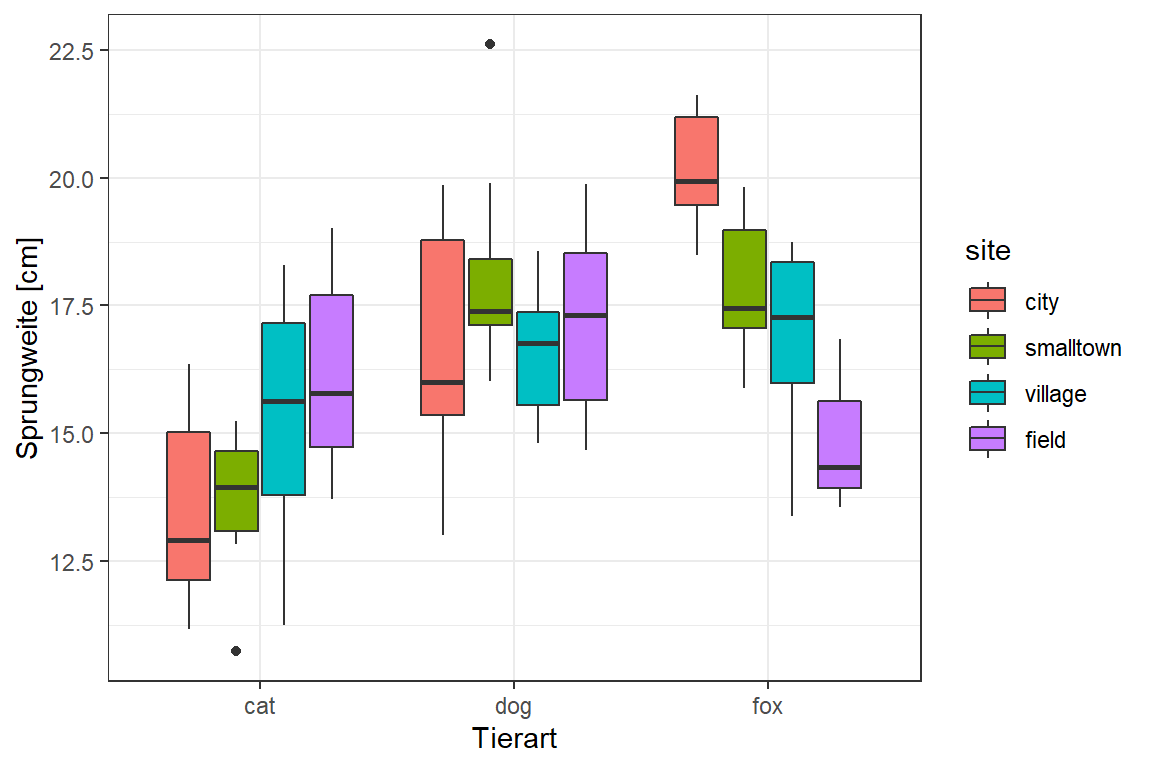
\includegraphics{./example-fleas-dogs-cats-foxes-site_files/figure-pdf/fig-example-4-1.pdf}

}

\caption{\label{fig-example-4}Boxplot der Sprungweiten {[}cm{]} für
Hunde-, Katzen- und Fuchsflöhe in verschiedenen Habitaten.}

\end{figure}

\begin{tcolorbox}[enhanced jigsaw, coltitle=black, titlerule=0mm, bottomrule=.15mm, opacityback=0, opacitybacktitle=0.6, leftrule=.75mm, title=\textcolor{quarto-callout-tip-color}{\faLightbulb}\hspace{0.5em}{Datei für von Flöhen auf Tieren in Habitaten}, toprule=.15mm, bottomtitle=1mm, toptitle=1mm, left=2mm, breakable, arc=.35mm, colback=white, rightrule=.15mm, colbacktitle=quarto-callout-tip-color!10!white, colframe=quarto-callout-tip-color-frame]
Du findest die Datei \texttt{flea\_dog\_cat\_fox\_site.xlsx} auf GitHub
\href{https://github.com/jkruppa/jkruppa.github.io/tree/master/data}{jkruppa.github.io/data/}
als Excel oder auch als CSV.
\end{tcolorbox}

\hypertarget{sec-example-5}{%
\chapter{Von vielen Flöhen auf Hunden und Katzen}\label{sec-example-5}}

\emph{Version vom September 14, 2022 um 08:45:38}

Wir schauen uns in diesem Beispiel wiederum nur zwei Tierarten an: Hunde
und Katzen. Auf diesen Tierarten messen wir wieder die Sprunglänge in
{[}cm{]} von jeweils 400 Tieren. Im Vergleich zu dem vorherigen Beispiel
erweitern wir die Daten um eine Spalte \texttt{jump\_weight} in {[}mg{]}
sowie \texttt{sex} {[}male, female{]}. Bei Versuch wurde noch in der
Variable \texttt{hatch\_time} gemessen, wie lange die Flöhe in Stunden
zum Schlümpfen brauchen. Es ergibt sich folgende
Tabelle~\ref{tbl-example-5} mit den ersten zehn Beobachtungen und die
dazugehörige Abbildung~\ref{fig-example-5}.

\hypertarget{tbl-example-5}{}
\begin{longtable}[]{@{}cccccc@{}}
\caption{\label{tbl-example-5}Sprunglängen {[}cm{]}, Gewichte {[}mg{]},
Geschecht {[}sex{]} und Schlüpfzeit {[}h{]} für Hunde- und
Katzenflöhe.}\tabularnewline
\toprule()
animal & sex & weight & jump\_length & flea\_count & hatch\_time \\
\midrule()
\endfirsthead
\toprule()
animal & sex & weight & jump\_length & flea\_count & hatch\_time \\
\midrule()
\endhead
cat & male & 6.02 & 15.79 & 5 & 483.60 \\
cat & male & 5.99 & 18.33 & 1 & 82.56 \\
cat & male & 8.05 & 17.58 & 1 & 296.73 \\
cat & male & 6.71 & 14.09 & 3 & 140.90 \\
cat & male & 6.19 & 18.22 & 1 & 162.20 \\
cat & male & 8.18 & 13.49 & 1 & 167.47 \\
cat & male & 7.46 & 16.28 & 1 & 291.20 \\
cat & male & 5.58 & 14.54 & 0 & 112.58 \\
cat & male & 6.19 & 16.36 & 1 & 143.97 \\
cat & male & 7.53 & 15.08 & 1 & 766.31 \\
\bottomrule()
\end{longtable}

{\marginnote{\begin{footnotesize}Über die explorative Datenanalyse
erfährst du mehr im Kapitel~\ref{sec-eda-ggplot}\end{footnotesize}}}

Die Datentabelle ist in dieser Form schon fast nicht mehr überschaubar.
Daher hilft hier die explorative Datenanalyse weiter. Wir schauen uns
daher die Daten einmal als einen Scatterplot in
Abbildung~\ref{fig-example-5} an. Wir sehen hier, dass wir das mit dem
Gewicht {[}mg{]} der Flöhe auch die Sprungweite in {[}cm{]} steigt.

\begin{figure}

{\centering 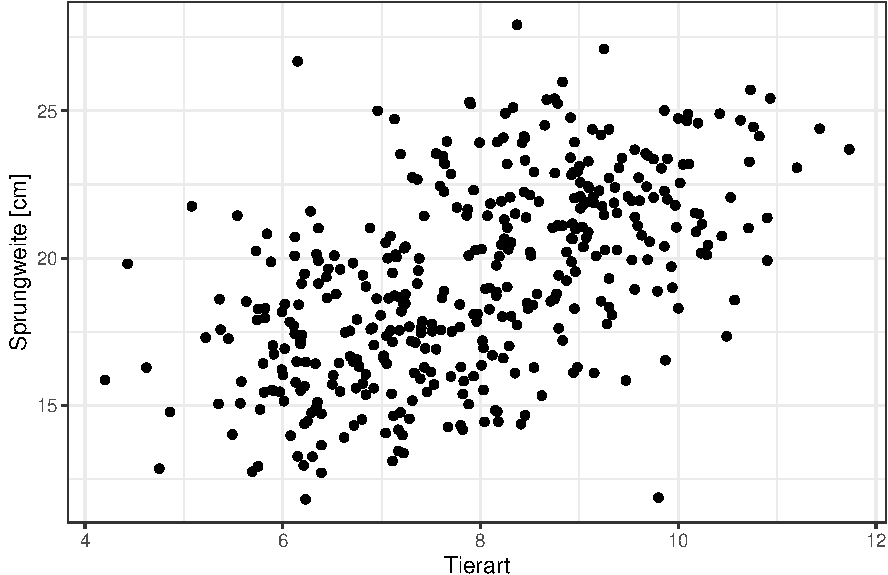
\includegraphics{./example-fleas-dogs-cats-length-weight_files/figure-pdf/fig-example-5-1.pdf}

}

\caption{\label{fig-example-5}Scatterplot der Sprunglängen {[}cm{]} und
Gewichte {[}mg{]} für Hunde- und Katzenflöhe.}

\end{figure}

\begin{tcolorbox}[enhanced jigsaw, coltitle=black, titlerule=0mm, bottomrule=.15mm, opacityback=0, opacitybacktitle=0.6, leftrule=.75mm, title=\textcolor{quarto-callout-tip-color}{\faLightbulb}\hspace{0.5em}{Datei für von vielen Flöhen auf Hunden und Katzen}, toprule=.15mm, bottomtitle=1mm, toptitle=1mm, left=2mm, breakable, arc=.35mm, colback=white, rightrule=.15mm, colbacktitle=quarto-callout-tip-color!10!white, colframe=quarto-callout-tip-color-frame]
Du findest die Datei \texttt{flea\_dog\_cat\_length\_weight.xlsx} auf
GitHub
\href{https://github.com/jkruppa/jkruppa.github.io/tree/master/data}{jkruppa.github.io/data/}
als Excel oder auch als CSV.
\end{tcolorbox}

\hypertarget{sec-example-gummibears}{%
\chapter{Gummibärchen}\label{sec-example-gummibears}}

\emph{Version vom September 14, 2022 um 08:45:45}

\begin{tcolorbox}[enhanced jigsaw, coltitle=black, titlerule=0mm, bottomrule=.15mm, opacityback=0, opacitybacktitle=0.6, leftrule=.75mm, title=\textcolor{quarto-callout-tip-color}{\faLightbulb}\hspace{0.5em}{Gummibärchen Daten und die explorative Datenanalyse}, toprule=.15mm, bottomtitle=1mm, toptitle=1mm, left=2mm, breakable, arc=.35mm, colback=white, rightrule=.15mm, colbacktitle=quarto-callout-tip-color!10!white, colframe=quarto-callout-tip-color-frame]
Du findest auf YouTube die
\href{https://youtu.be/gEwOmvWvdxo}{Gummibärchen Daten und die
explorative Datenanalyse} als Video. Vielleicht interessiert es dich mal
so eine Auswertung im Video anzuschauen.
\end{tcolorbox}

\marginnote{\begin{footnotesize}

Wenn dich der Ablauf technisch interssiert findet du unter Kruppa und
Sieg (2021) mehr Informationen dazu.

\end{footnotesize}}

Im Folgenden sehen wir in Tabelle~\ref{tbl-gummi} den Gummibärchen
Datensatz, der im Laufe der letzten Jahre entstanden ist. Dabei wächst
der Datensatz von Semester zu Semester immer ein wenig weiter. Jedes
Semester darf Tütchen aufreißen und schauen was da so drin ist.

\hypertarget{tbl-gummi}{}
\begin{table*}

\begin{longtable}[]{@{}
  >{\centering\arraybackslash}p{(\columnwidth - 28\tabcolsep) * \real{0.0397}}
  >{\centering\arraybackslash}p{(\columnwidth - 28\tabcolsep) * \real{0.1788}}
  >{\centering\arraybackslash}p{(\columnwidth - 28\tabcolsep) * \real{0.0596}}
  >{\centering\arraybackslash}p{(\columnwidth - 28\tabcolsep) * \real{0.0662}}
  >{\centering\arraybackslash}p{(\columnwidth - 28\tabcolsep) * \real{0.0530}}
  >{\centering\arraybackslash}p{(\columnwidth - 28\tabcolsep) * \real{0.0530}}
  >{\centering\arraybackslash}p{(\columnwidth - 28\tabcolsep) * \real{0.0464}}
  >{\centering\arraybackslash}p{(\columnwidth - 28\tabcolsep) * \real{0.0464}}
  >{\centering\arraybackslash}p{(\columnwidth - 28\tabcolsep) * \real{0.0861}}
  >{\centering\arraybackslash}p{(\columnwidth - 28\tabcolsep) * \real{0.0861}}
  >{\centering\arraybackslash}p{(\columnwidth - 28\tabcolsep) * \real{0.0795}}
  >{\centering\arraybackslash}p{(\columnwidth - 28\tabcolsep) * \real{0.0530}}
  >{\centering\arraybackslash}p{(\columnwidth - 28\tabcolsep) * \real{0.0331}}
  >{\centering\arraybackslash}p{(\columnwidth - 28\tabcolsep) * \real{0.0530}}
  >{\centering\arraybackslash}p{(\columnwidth - 28\tabcolsep) * \real{0.0662}}@{}}
\caption{\label{tbl-gummi}Auszug aus dem Daten zu den
Gummibärchendaten.}\tabularnewline
\toprule()
\begin{minipage}[b]{\linewidth}\centering
year
\end{minipage} & \begin{minipage}[b]{\linewidth}\centering
module
\end{minipage} & \begin{minipage}[b]{\linewidth}\centering
darkred
\end{minipage} & \begin{minipage}[b]{\linewidth}\centering
lightred
\end{minipage} & \begin{minipage}[b]{\linewidth}\centering
orange
\end{minipage} & \begin{minipage}[b]{\linewidth}\centering
yellow
\end{minipage} & \begin{minipage}[b]{\linewidth}\centering
green
\end{minipage} & \begin{minipage}[b]{\linewidth}\centering
white
\end{minipage} & \begin{minipage}[b]{\linewidth}\centering
count\_bears
\end{minipage} & \begin{minipage}[b]{\linewidth}\centering
count\_color
\end{minipage} & \begin{minipage}[b]{\linewidth}\centering
most\_liked
\end{minipage} & \begin{minipage}[b]{\linewidth}\centering
gender
\end{minipage} & \begin{minipage}[b]{\linewidth}\centering
age
\end{minipage} & \begin{minipage}[b]{\linewidth}\centering
height
\end{minipage} & \begin{minipage}[b]{\linewidth}\centering
semester
\end{minipage} \\
\midrule()
\endfirsthead
\toprule()
\begin{minipage}[b]{\linewidth}\centering
year
\end{minipage} & \begin{minipage}[b]{\linewidth}\centering
module
\end{minipage} & \begin{minipage}[b]{\linewidth}\centering
darkred
\end{minipage} & \begin{minipage}[b]{\linewidth}\centering
lightred
\end{minipage} & \begin{minipage}[b]{\linewidth}\centering
orange
\end{minipage} & \begin{minipage}[b]{\linewidth}\centering
yellow
\end{minipage} & \begin{minipage}[b]{\linewidth}\centering
green
\end{minipage} & \begin{minipage}[b]{\linewidth}\centering
white
\end{minipage} & \begin{minipage}[b]{\linewidth}\centering
count\_bears
\end{minipage} & \begin{minipage}[b]{\linewidth}\centering
count\_color
\end{minipage} & \begin{minipage}[b]{\linewidth}\centering
most\_liked
\end{minipage} & \begin{minipage}[b]{\linewidth}\centering
gender
\end{minipage} & \begin{minipage}[b]{\linewidth}\centering
age
\end{minipage} & \begin{minipage}[b]{\linewidth}\centering
height
\end{minipage} & \begin{minipage}[b]{\linewidth}\centering
semester
\end{minipage} \\
\midrule()
\endhead
2018 & NA & 0 & 0 & 5 & 4 & 0 & 0 & 9 & 3 & lightred & m & 35 & 193 &
10 \\
2018 & NA & 0 & 3 & 1 & 4 & 1 & 1 & 10 & 5 & yellow & w & 21 & 159 &
6 \\
2018 & NA & 1 & 2 & 2 & 2 & 1 & 1 & 9 & 6 & white & w & 21 & 159 & 6 \\
2018 & NA & 2 & 0 & 2 & 1 & 2 & 3 & 10 & 5 & white & w & 36 & 180 &
10 \\
2018 & NA & 2 & 1 & 1 & 2 & 2 & 2 & 10 & 6 & white & m & 22 & 180 & 3 \\
2018 & NA & 2 & 4 & 1 & 2 & 0 & 1 & 10 & 5 & white & m & NA & NA & NA \\
\ldots{} & \ldots{} & \ldots{} & \ldots{} & \ldots{} & \ldots{} &
\ldots{} & \ldots{} & \ldots{} & \ldots{} & \ldots{} & \ldots{} &
\ldots{} & \ldots{} & \ldots{} \\
2022 & Fakultaetsinformationstag & 2 & 1 & 1 & 2 & 4 & 2 & 12 & 5 &
darkred & w & 46 & 165 & 0 \\
2022 & Fakultaetsinformationstag & 2 & 0 & 0 & 5 & 0 & 3 & 10 & 2 &
darkred & w & 55 & 177 & 0 \\
2022 & Fakultaetsinformationstag & 2 & 2 & 2 & 2 & 0 & 1 & 9 & 5 & green
& w & 46 & 173 & 0 \\
2022 & Fakultaetsinformationstag & 4 & 1 & 1 & 1 & 1 & 4 & 12 & 6 &
white & w & 21 & 168 & 0 \\
2022 & Fakultaetsinformationstag & 1 & 0 & 1 & 2 & 2 & 2 & 8 & 5 & green
& m & 24 & 183 & 0 \\
2022 & Fakultaetsinformationstag & 0 & 3 & 2 & 1 & 0 & 2 & 9 & 5 &
darkred & w & 21 & 171 & 0 \\
\bottomrule()
\end{longtable}

\end{table*}

Wir erheben folgende Variablen im Datensatz. Dabei unterscheiden wir
einmal in Daten, die technischer Natur sind:

\begin{itemize}
\tightlist
\item
  \textbf{year}, das Jahr in dem die Daten erhoben wurden.
\item
  \textbf{module}, das Module in welchem die Daten erhoben wurden. Am
  Anfang wurde das Modul noch nicht erfasst.
\item
  \textbf{darkred} bis \textbf{white}, die Anzahl an Gummibärchen in der
  jeweiligen Farbe.
\item
  \textbf{count\_bears}, die Anzahl an Gummibärchen in der
  entsprechenden Tüte.
\item
  \textbf{count\_color}, die Anzahl an Farben und damit
  Geschmacksrichtungen in einer Tüte.
\end{itemize}

Dann wollen wir aber auch noch etwas über den Studierenden wissen, der
die Tüte aufgemacht hat. Wir erheben hier noch einge demographische
Informationen:

\begin{itemize}
\tightlist
\item
  \textbf{most\_liked}, der Lieblingsgeschmack des Studierenden.
\item
  \textbf{gender}, das Geschlecht des Studierenden. Aktuell gibt es nur
  männlich oder weiblich Studierende.
\item
  \textbf{age}, das Alter in Jahren {[}y{]} der Studierenden.
\item
  \textbf{height}, die Körpergröße des Studierenden in {[}cm{]}
\item
  \textbf{semester}, das aktuelle Semester des Studierenden. Wir
  unterscheiden nicht zwischen Bachelor und Master
\end{itemize}

Aktuell hat der Datensatz \(n = 315\) Beobachtungen. Da der Datensatz
aber immer weiter wächst brauchen wir wirklich R dazu um den Datensatz
uns anschauen zu können.

\begin{tcolorbox}[enhanced jigsaw, coltitle=black, titlerule=0mm, bottomrule=.15mm, opacityback=0, opacitybacktitle=0.6, leftrule=.75mm, title=\textcolor{quarto-callout-tip-color}{\faLightbulb}\hspace{0.5em}{Datei für von Flöhen, Hunden und Katzen}, toprule=.15mm, bottomtitle=1mm, toptitle=1mm, left=2mm, breakable, arc=.35mm, colback=white, rightrule=.15mm, colbacktitle=quarto-callout-tip-color!10!white, colframe=quarto-callout-tip-color-frame]
Du findest die Datei \texttt{gummibears.xlsx} auf GitHub
\href{https://github.com/jkruppa/jkruppa.github.io/tree/master/data}{jkruppa.github.io/data/}
als Excel Datei.
\end{tcolorbox}

\hypertarget{referenzen-1}{%
\section*{Referenzen}\label{referenzen-1}}
\addcontentsline{toc}{section}{Referenzen}

\part{Programmieren in R}

\emph{Version vom September 14, 2022 um 08:45:52}

Was solltest du nun zuerst Lesen? Es ist sehr schwierig die
Programmierung exakt so zu schreiben, dass das Programmieren
\emph{linear} verständlich ist. Du brauchst im Prinzip das Wissen aus
Kapitel~\ref{sec-basics} \emph{Operatoren, Funktionen und Pakete} um die
Grundlagen zu verstehen. Auf der anderen Seite fehlt dir vielleicht noch
das Verständnis von Buchstaben und Zahlen in R. Diesen Zusammenhang
zwischen Buchstaben und Zahlen erkläre ich als erstes im folgenden
Kapitel~\ref{sec-letter-number} \emph{Von Buchstaben und Zahlen}.

Im vorherigen Kapitel zu den Beispielen haben wir die Datentabelle
Tabelle~\ref{tbl-dog-cat-long} mit den Hunde- und Katzenflöhen
erschaffen. Bevor wir uns weiter mit statistischen Kennzahlen
beschäftigen, wollen wir uns einmal die Realisierung der Tabelle
Tabelle~\ref{tbl-dog-cat-long} mit den Hunde- und Katzenflöhen in R
anschauen. Dabei wollen wir auch Eigenschaften von Zahlen und Buchstaben
lernen, die notwendig sind um mit einem Programm wie R kommunizieren zu
können. Wir wollen später R nutzen um die explorative Datenanalyse
anzuwenden. Über die explorative Datenanalyse lernen wir in späteren
Kapiteln mehr.

\begin{tcolorbox}[enhanced jigsaw, coltitle=black, titlerule=0mm, bottomrule=.15mm, opacityback=0, opacitybacktitle=0.6, leftrule=.75mm, title=\textcolor{quarto-callout-tip-color}{\faLightbulb}\hspace{0.5em}{Einführung in R per Video}, toprule=.15mm, bottomtitle=1mm, toptitle=1mm, left=2mm, breakable, arc=.35mm, colback=white, rightrule=.15mm, colbacktitle=quarto-callout-tip-color!10!white, colframe=quarto-callout-tip-color-frame]
Du findest auf YouTube
\href{https://www.youtube.com/playlist?list=PLe51bCp9JvEFUnFqaJG5aRmON9i1ZbOYC}{Grundlagen
in R} als Video Reihe. Ich werde zwar alles nochmal hier als Text
aufschreiben, aber manchmal ist das Sehen und Hören dann einfacher.
\end{tcolorbox}

\hypertarget{sec-letter-number}{%
\chapter{Von Buchstaben und Zahlen}\label{sec-letter-number}}

\emph{Version vom September 14, 2022 um 08:45:59}

Im Kapitel~\ref{sec-example-2} haben wir uns die Sprungweiten und andere
Eigenschaften von Hunden und Katzen angeschaut. Bevor wir uns weiter mit
statistischen Kennzahlen beschäftigen, wollen wir uns einmal die
Realisierung der Tabelle~\ref{tbl-dog-cat-letter} in R anschauen. Das
heist, wie ist eine Tabelle in R aufgebaut und was sehen wir da
eigentlich?

\hypertarget{tbl-dog-cat-letter}{}
\begin{longtable}[]{@{}ccccc@{}}
\caption{\label{tbl-dog-cat-letter}Sprunglängen {[}cm{]} für Hunde- und
Katzenflöhe.}\tabularnewline
\toprule()
animal & jump\_length & flea\_count & grade & infected \\
\midrule()
\endfirsthead
\toprule()
animal & jump\_length & flea\_count & grade & infected \\
\midrule()
\endhead
dog & 5.7 & 18 & 8 & FALSE \\
dog & 8.9 & 22 & 8 & TRUE \\
dog & 11.8 & 17 & 6 & TRUE \\
dog & 8.2 & 12 & 8 & FALSE \\
dog & 5.6 & 23 & 7 & TRUE \\
dog & 9.1 & 18 & 7 & FALSE \\
dog & 7.6 & 21 & 9 & FALSE \\
cat & 3.2 & 12 & 7 & TRUE \\
cat & 2.2 & 13 & 5 & FALSE \\
cat & 5.4 & 11 & 7 & FALSE \\
cat & 4.1 & 12 & 6 & FALSE \\
cat & 4.3 & 16 & 6 & TRUE \\
cat & 7.9 & 9 & 6 & FALSE \\
cat & 6.1 & 7 & 5 & FALSE \\
\bottomrule()
\end{longtable}

Dabei wollen wir auch Eigenschaften von Zahlen und Buchstaben lernen,
die notwendig sind um mit einem Programm wie R kommunizieren zu können.
Nun haben wir in der Tabelle~\ref{tbl-dog-cat-letter} mit Daten zu
verschiedenen Oucomes, wie Sprungweite {[}cm{]}, Anzahl an Flöhen auf
Hunden und Katzen, die Boniturnoten oder aber den Infektionsstatus. Die
Tabelle ist zwar nicht groß aber auch nicht wirklich klein. Wir wollen
uns nun damit beschäftigen, die Zahlen sinnvoll in R darzustellen. Wir
wollen mit der Darstellung einer Datentabelle in R beginnen, einem
\texttt{tibble()}.

\hypertarget{daten-in-r-sind-tibble}{%
\section{\texorpdfstring{Daten in R sind
\texttt{tibble()}}{Daten in R sind tibble()}}\label{daten-in-r-sind-tibble}}

Im folgenden sehen wir die Daten aus der
Tabelle~\ref{tbl-dog-cat-letter} in R als \texttt{tibble} dargestellt.
Was ist nun ein \texttt{tibble}? Ein \texttt{tibble} ist zu aller erst
ein Speicher für Daten in R. Das heist wir haben Spalten und Zeilen.
Jede Spalte repräsentiert eine Messung oder Variable und die Zeilen
jeweils eine Beobachtung.

\begin{verbatim}
# A tibble: 14 x 5
   animal jump_length flea_count grade infected
   <chr>        <dbl>      <int> <dbl> <lgl>   
 1 dog            5.7         18     8 FALSE   
 2 dog            8.9         22     8 TRUE    
 3 dog           11.8         17     6 TRUE    
 4 dog            8.2         12     8 FALSE   
 5 dog            5.6         23     7 TRUE    
 6 dog            9.1         18     7 FALSE   
 7 dog            7.6         21     9 FALSE   
 8 cat            3.2         12     7 TRUE    
 9 cat            2.2         13     5 FALSE   
10 cat            5.4         11     7 FALSE   
11 cat            4.1         12     6 FALSE   
12 cat            4.3         16     6 TRUE    
13 cat            7.9          9     6 FALSE   
14 cat            6.1          7     5 FALSE   
\end{verbatim}

Als erstes erfahren wir, dass wir einen \texttt{A\ tibble:\ 14\ x\ 5}
vorliegen haben. Das heist, wir haben 14 Zeile und 5 Spalten. In einem
\texttt{tibble} wird immer in der ersten Zeile angezeigt wieviele
Beobachtungen wir in dem Datensatz haben. Wenn das \texttt{tibble} zu
groß wird, werden wir nicht mehr das ganze \texttt{tibble} sehen sondern
nur noch einen Ausschnitt. Im Weiteren hat jede Spalte noch eine
Eigenschaft unter dem Spaltennamen:

\begin{itemize}
\tightlist
\item
  \texttt{\textless{}chr\textgreater{}} bedeutet \texttt{character}. Wir
  haben also hier Worte vorliegen.
\item
  \texttt{\textless{}dbl\textgreater{}} bedeutet \texttt{double}. Ein
  \texttt{double} ist eine Zahl mit Kommastellen.
\item
  \texttt{\textless{}int\textgreater{}} bedeutet \texttt{integer}. Ein
  \texttt{integer} ist eine ganze Zahl ohne Kommastellen.
\item
  \texttt{\textless{}lgl\textgreater{}} bedeutet \texttt{logical} oder
  \texttt{boolean}. Hier gibt es nur die Ausprägung \emph{wahr} oder
  \emph{falsch}. Somit \texttt{TRUE} oder \texttt{FALSE}. Statt den
  Worten \texttt{TRUE} oder \texttt{FALSE} kann hier auch 0 oder 1
  stehen.
\item
  \texttt{\textless{}str\textgreater{}} bedeutet \texttt{string} der aus
  verschiedenen \texttt{character} besteht kann, getrennt durch
  Leerzeichen.
\end{itemize}

\begin{tcolorbox}[enhanced jigsaw, coltitle=black, titlerule=0mm, bottomrule=.15mm, opacityback=0, opacitybacktitle=0.6, leftrule=.75mm, title=\textcolor{quarto-callout-tip-color}{\faLightbulb}\hspace{0.5em}{Zahlen, Buchstaben, Skalenniveau - Was ist das eigentlich?}, toprule=.15mm, bottomtitle=1mm, toptitle=1mm, left=2mm, breakable, arc=.35mm, colback=white, rightrule=.15mm, colbacktitle=quarto-callout-tip-color!10!white, colframe=quarto-callout-tip-color-frame]
Du findest auf YouTube \href{https://youtu.be/OnRaSmybhOQ}{Einführung in
R - Teil 06 - Zahlen, Buchstaben, Skalenniveau - Was ist das
eigentlich?} als Video. Hier erkläre ich den Zusammenhang nochmal in
einem Video.
\end{tcolorbox}

\hypertarget{faktoren-als-wuxf6rter-zu-zahlen}{%
\section{Faktoren als Wörter zu
Zahlen}\label{faktoren-als-wuxf6rter-zu-zahlen}}

{\marginnote{\begin{footnotesize}Ein \textbf{Faktor} ist eine Variable
mit mehrern \textbf{Faktorstufen} oder \textbf{Leveln}. Für uns sieht
der Faktor wie ein Wort aus, hinter jedem Wort steht aber eine Zahl mit
der gerechnet werden kann.\end{footnotesize}}}

Ein Computer und somit auch eine Programmsprache wie R kann keine
Buchstaben \emph{verrechnen}. Ein Programm kann nur mit Zahlen rechnen.
Wir haben aber in der Tabelle~\ref{tbl-dog-cat-letter} in der Spalte
\texttt{animal} Buchstaben stehen. Da wir hier einen Kompromiss eingehen
müssen führen wir Faktoren ein. Ein Faktor kombiniert Buchstaben mit
Zahlen. Wir als Anwender sehen die Buchstaben, die Wörter bilden. Intern
steht aber jedes Wort für eine Zahl, so dass R mit den Zahlen rechnen
kann. Klingt ein wenig kryptisch, aber wir schauen uns einen
\texttt{factor} einmal an.

\begin{Shaded}
\begin{Highlighting}[]
\NormalTok{data\_tbl}\SpecialCharTok{$}\NormalTok{animal[}\DecValTok{1}\SpecialCharTok{:}\DecValTok{8}\NormalTok{]}
\end{Highlighting}
\end{Shaded}

\begin{verbatim}
[1] "dog" "dog" "dog" "dog" "dog" "dog" "dog" "cat"
\end{verbatim}

Was haben wir gemacht? Als erstes haben wir die Spalte \texttt{animal}
aus dem Datensatz \texttt{data\_tbl} mit dem Dollarzeichen \texttt{\$}
\emph{herausgezogen}. Mit dem \texttt{\$} Zeichen können wir uns eine
einzelne Spalte aus dem Datensatz \texttt{data\_tbl} rausziehen. Du
kannst dir das \texttt{\$} wie einen Kleiderbügel und das
\texttt{data\_tbl} als einen Schrank für Kleiderbügel verstellen. An dem
Kleiderbügel hängen dann die einzelnen Zahlen und Worte. Wir nehmen aber
nicht den ganzen Vektor sondern nur die Zahlen 1 bis 8, dargestellt
durch \texttt{{[}1:8{]}}. Die Gänsefüße \texttt{"} um \texttt{dog}
zeigen uns, dass wir hier Wörter oder \texttt{character}vorliegen haben.
Schauen wir auf das Ergebnis, so erhalten wir sieben Mal \texttt{dog}
und einmal \texttt{cat}. Insgesamt die ersten acht Einträge der
Datentabelle. Wir wollen diesen Vektor uns nun einmal als Faktor
anschauen. Wir nutzen die Funktion \texttt{as\_factor()}.
{\marginnote{\begin{footnotesize}Über Funktionen kannst du im
Kapitel~\ref{sec-R-function} mehr erfahren.\end{footnotesize}}}

\begin{Shaded}
\begin{Highlighting}[]
\FunctionTok{as.factor}\NormalTok{(data\_tbl}\SpecialCharTok{$}\NormalTok{animal[}\DecValTok{1}\SpecialCharTok{:}\DecValTok{8}\NormalTok{])}
\end{Highlighting}
\end{Shaded}

\begin{verbatim}
[1] dog dog dog dog dog dog dog cat
Levels: cat dog
\end{verbatim}

Im direkten vergleich verschwinden die Gänsefüße \texttt{"} um
\texttt{dog} und zeigen usn, dass wir hier keine \texttt{character} mehr
vorliegen haben. Darüber hinaus sehen wir auch, dass die der Faktor
jetzt \texttt{Levels} hat. Exakt zwei Stück. Jeweils einen für
\texttt{dog} und einen für \texttt{cat}. Wir werden später Faktoren
benötigen, wenn wir zum Beispiel eine einfaktorielle ANOVA rechnen. Hier
siehst du schon den Begriff \emph{Faktor} wieder.

\marginnote{\begin{footnotesize}

Wir brauchen später zum Modellieren einen Datensatz, der \emph{meist}
aus einer \textbf{Outcome}-Spalte, einer \textbf{Faktor}-Spalte mit der
\emph{Behandlung} und einer \textbf{Faktor}-Spalte mit dem \emph{Block}
oder \emph{Cluster} besteht.

\[
{\small Outcome \sim Behandlung + Block}
\]

\end{footnotesize}}

\hypertarget{von-wuxf6rtern-und-objekten}{%
\section{Von Wörtern und Objekten}\label{von-wuxf6rtern-und-objekten}}

Das mag etwas verwirrend sein, denn es gibt in R Wörter
\texttt{string\ \textless{}str\textgreater{}} oder
\texttt{character\ \textless{}chr\textgreater{}}. Wörter sind was
anderes als Objekte. Streng genommen sind beides Wörter, aber in
Objekten werden Dinge gespeichert wohin gegen das Wort einfach ein Wort
ist. Deshalb kennezeichnen wir Wörter auch mit Gänsefüßchen als win
\texttt{"wort"} und zeigen damit, dass es sich hier um einen String
handelt.

Wir tippen \texttt{"animal"} in R und erhalten \texttt{"animal"} als
Wort zurück. Das sehen wir auch an dem Ausdruck mit den Gänsefüßchen.

\begin{Shaded}
\begin{Highlighting}[]
\StringTok{"animal"}
\end{Highlighting}
\end{Shaded}

\begin{verbatim}
[1] "animal"
\end{verbatim}

{\marginnote{\begin{footnotesize}Über den Zuweisungspfeil
\texttt{\textless{}-} kannst du im Kapitel~\ref{sec-R-pfeil} mehr
erfahren.\end{footnotesize}}}

Wir tippen \texttt{animal} ohne die Anführungszeichen in R und erhalten
den Inhalt von \texttt{animal} ausgegeben. Dafür müssen wir aber das
Objekt \texttt{animal} erst einmal über den Zuweisungspfeil
\texttt{\textless{}-}erschaffen.

\begin{Shaded}
\begin{Highlighting}[]
\NormalTok{animal }\OtherTok{\textless{}{-}} \FunctionTok{c}\NormalTok{(}\StringTok{"dog"}\NormalTok{, }\StringTok{"cat"}\NormalTok{, }\StringTok{"fox"}\NormalTok{)}
\NormalTok{animal}
\end{Highlighting}
\end{Shaded}

\begin{verbatim}
[1] "dog" "cat" "fox"
\end{verbatim}

Sollte es das Objekt \texttt{animal} nicht geben, also nicht über den
Zuweisungspfeil \texttt{\textless{}-} erschaffen worden, dann wird eine
Fehlermeldung von R ausgegeben:

\texttt{Fehler\ in\ eval(expr,\ envir,\ enclos)\ :\ Objekt\ \textquotesingle{}animal\textquotesingle{}\ nicht\ gefunden}

\hypertarget{zusammenfassung}{%
\section{Zusammenfassung}\label{zusammenfassung}}

{\marginnote{\begin{footnotesize}\textbf{Variablennamen} meint hier
immer den \textbf{Namen der Spalte} im Datensatz bzw.
\texttt{tibble}\end{footnotesize}}}

Tabelle~\ref{tbl-skalenniveau} zeigt eine Übersicht wie einzelne
Variablennamen und deren zugehörigen Beispielen sowie den Namen in R,
der Informatik allgemein, als Skalenneivau und welcher
Verteilungsfamilie die Variable angehören würde. Leider ist es so, dass
wieder gleiche Dinge unterschiedliche benannt werden. Aber an dieses
doppelte Benennen können wir uns in der Statistik schonmal gewöhnen.

\begin{figure*}

\hypertarget{tbl-skalenniveau}{}
\begin{longtable}[]{@{}
  >{\raggedright\arraybackslash}p{(\columnwidth - 10\tabcolsep) * \real{0.1200}}
  >{\raggedright\arraybackslash}p{(\columnwidth - 10\tabcolsep) * \real{0.2320}}
  >{\raggedright\arraybackslash}p{(\columnwidth - 10\tabcolsep) * \real{0.0880}}
  >{\raggedright\arraybackslash}p{(\columnwidth - 10\tabcolsep) * \real{0.1440}}
  >{\raggedright\arraybackslash}p{(\columnwidth - 10\tabcolsep) * \real{0.2560}}
  >{\raggedright\arraybackslash}p{(\columnwidth - 10\tabcolsep) * \real{0.1600}}@{}}
\caption{\label{tbl-skalenniveau}Zusammenfassung und Übersicht von
Variablennamen und deren Bennung in R, in der Informatik allgemein, als
Skalenniveau und die dazugehörige Verteilungsfamilie.}\tabularnewline
\toprule()
\begin{minipage}[b]{\linewidth}\raggedright
Variablenname
\end{minipage} & \begin{minipage}[b]{\linewidth}\raggedright
Beispiel
\end{minipage} & \begin{minipage}[b]{\linewidth}\raggedright
R
\end{minipage} & \begin{minipage}[b]{\linewidth}\raggedright
Infomatik
\end{minipage} & \begin{minipage}[b]{\linewidth}\raggedright
Skalenniveau
\end{minipage} & \begin{minipage}[b]{\linewidth}\raggedright
Verteilungsfamilie
\end{minipage} \\
\midrule()
\endfirsthead
\toprule()
\begin{minipage}[b]{\linewidth}\raggedright
Variablenname
\end{minipage} & \begin{minipage}[b]{\linewidth}\raggedright
Beispiel
\end{minipage} & \begin{minipage}[b]{\linewidth}\raggedright
R
\end{minipage} & \begin{minipage}[b]{\linewidth}\raggedright
Infomatik
\end{minipage} & \begin{minipage}[b]{\linewidth}\raggedright
Skalenniveau
\end{minipage} & \begin{minipage}[b]{\linewidth}\raggedright
Verteilungsfamilie
\end{minipage} \\
\midrule()
\endhead
weight & 12.3, 12.4, 5.4, 21.3, 13.4 & numeric & double & continuous &
Gaussian \\
count & 5, 0, 12, 23, 1, 4, 21 & integer & integer & discrete &
Poisson \\
dosis & low, mid, high & ordered & & categorical / ordinal & Ordinal \\
field & mainz, berlin, kiel & factor & & categorical & Multinomial \\
cancer & 0, 1 & factor & & dichotomous / binary / nominal & Binomial \\
treatment & ``placebo'', ``aspirin'' & character & character/string &
dichotomous / binary / nominal & Binomial \\
birth & 2001-12-02, 2005-05-23 & date & & & \\
\bottomrule()
\end{longtable}

\end{figure*}

\hypertarget{sec-basics}{%
\chapter{Operatoren, Funktionen und Pakete}\label{sec-basics}}

\emph{Version vom September 14, 2022 um 08:46:11}

Es ist immer schwierig, wann die Grundlagen von R einmal gelehrt werden
sollte. Wenn du nichts von Programmierung bis jetzt gehört hast, dann
mag es keinen Sinn ergeben mit Operatoren, wie dem Zuweisungspfeil
\texttt{\textless{}-} und der Pipe \texttt{\%\textgreater{}\%} zu
beginnen. Wir brauchen aber für die Programmierung folgende zentrale
Konzepte.

\begin{itemize}
\tightlist
\item
  Wir müssen zusätzliche Pakete in R installieren und laden können
  (siehe Kapitel~\ref{sec-R-packages}).
\item
  Wir müssen verstehen wie wir uns einen Vektor mit \texttt{c()} bauen
  (siehe Kapitel~\ref{sec-R-vector}).
\item
  Wir müssen wissen was eine Funktion in R ist (siehe
  Kapitel~\ref{sec-R-function}).
\item
  Wir müssen den Operator Zuweisungspfeil \texttt{\textless{}-}
  verstehen und anwenden können (siehe Kapitel~\ref{sec-R-pfeil}).
\item
  Wir müssen den Operator Pipe \texttt{\%\textgreater{}\%} verstehen und
  anwenden können (siehe Kapitel~\ref{sec-R-pipe}).
\item
  Wir müssen den Operator \texttt{\$} verstehen, da manche Funktionen in
  R nicht mit Datensätzen sondenr nur mit Vektoren arbeiten können
  (siehe Kapitel~\ref{sec-dollar}).
\item
  Wir müssen verstehen wie wir ein Modell in R mit der Tilde
  \texttt{\textasciitilde{}} definieren (siehe
  Kapitel~\ref{sec-formula}).
\item
  Wir müssen wissen und verstehen wie wir mit \texttt{?} englische
  Hilfeseiten öffnen können (siehe Kapitel~\ref{sec-R-help}).
\end{itemize}

Nicht alle Konzepte brauchst du \emph{unmittelbar} aber ich nutze diese
Konzepte wiederholt in allen Kapiteln, so dass du hier immer wieder mal
schauen kannst, was die Grundlagen sind.

\hypertarget{sec-R-packages}{%
\section{\texorpdfstring{Pakete und
\texttt{library()}}{Pakete und library()}}\label{sec-R-packages}}

{\marginnote{\begin{footnotesize}Als Vanilla beschreibt man in der
Informatikerwelt ein Programm, was keine zusätzlichen Pakete geladen
hat. Also die reinst Form ohne zusätzlichen
Geschmack.\end{footnotesize}}}

In der \emph{Vanilla}-Variante hat R sehr wenige Funktionen. Ohne
zusätzliche Pakete ist R mehr ein sehr potenter Taschenrechner. Leider
mit der Funktionalität aus den 90'zigern, was die Programmierumgebung
und die Funktionen angeht. Das wollen wir aber nicht. Wir wollen auf den
aktuellen Stand der Technik und auch Sprache programmieren. Daher nutzen
wir zusätzliche R Pakete.

\begin{figure}

{\centering 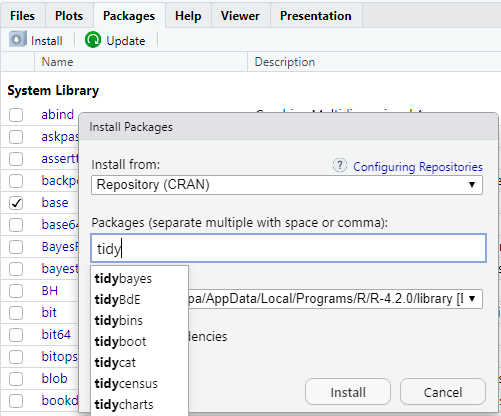
\includegraphics[width=0.8\textwidth,height=\textheight]{./images/programing_01.PNG}

}

\caption{\label{fig-pro-01}Auf den Reiter \emph{Packages} klicken und
dann \emph{Install}. In der deutschen version vom RStudio mögen die
Begriffe leicht anders sein.}

\end{figure}

In Abbildung~\ref{fig-pro-01} wird gezeigt wie du ein zusätzliches Paket
installieren kannst. Hierbei ist nochmal wichtig den semantischen
Unterschied zu wissen. Es gibt das Paket \texttt{tidyverse} was wir viel
nutzen. Wir isnatllieren \emph{einmalig} Pakete der Funktion
\texttt{install.packages()} oder eben wie in Abbildung~\ref{fig-pro-01}
gezeigt. Wir nutzen die Funktion \texttt{library()} um ein Paket in R zu
laden. Ja, es müsste anders heisen, tut es aber nicht.

\begin{Shaded}
\begin{Highlighting}[]
\DocumentationTok{\#\# Das Paket tidyverse installieren {-} einmalig}
\FunctionTok{install.packages}\NormalTok{(tidyverse)}

\DocumentationTok{\#\# Das Paket tidyverse laden {-} jedes Mal}
\FunctionTok{library}\NormalTok{(tidyverse)}
\end{Highlighting}
\end{Shaded}

Nun muss man sich immer merken, ob das Paket schon installiert ist oder
man schreibt relativ viele \texttt{library()} untereinander. Das
passiert schnell, wenn du viele Pakete laden willst. Dafür erlaubt dir
das Paket \texttt{pacman} eine Vereinfachung. Die Funktion
\texttt{p\_load()} installiert Pakete, wenn die Pakete nicht installiert
sind. Sollten die Pakete installiert sein, so werden die Pakete geladen.
Du musst nur einmal \texttt{install.packages(pacman)} ausführen um das
Paket \texttt{pacman} zu installieren.

\begin{Shaded}
\begin{Highlighting}[]
\NormalTok{pacman}\SpecialCharTok{::}\FunctionTok{p\_load}\NormalTok{(tidyverse, magrittr, readxl)}
\end{Highlighting}
\end{Shaded}

Schlussendlich gibt es noch die Möglichkeit sich alles nochmal bei
YouTube anzuschauen.

\begin{tcolorbox}[enhanced jigsaw, coltitle=black, titlerule=0mm, bottomrule=.15mm, opacityback=0, opacitybacktitle=0.6, leftrule=.75mm, title=\textcolor{quarto-callout-tip-color}{\faLightbulb}\hspace{0.5em}{Unterschied von Packages und Libraries in R}, toprule=.15mm, bottomtitle=1mm, toptitle=1mm, left=2mm, breakable, arc=.35mm, colback=white, rightrule=.15mm, colbacktitle=quarto-callout-tip-color!10!white, colframe=quarto-callout-tip-color-frame]
Du findest auf YouTube \href{https://youtu.be/TWimhd3ZyMM}{Einführung in
R - Teil 03 - Unterschied Packages und Libraries in R} als Video. Hier
erkläre ich nochmal den Ablauf zwischen Installieren eines Paketes und
dem Laden eines Paketes.
\end{tcolorbox}

\hypertarget{sec-R-vector}{%
\section{\texorpdfstring{Einen Vektor bauen
\texttt{c()}}{Einen Vektor bauen c()}}\label{sec-R-vector}}

Wir können mit der Funktion \texttt{c()} Zahlen und Wörter zu einem
Vektor kombinieren.

\begin{Shaded}
\begin{Highlighting}[]
\FunctionTok{c}\NormalTok{(}\StringTok{"dog"}\NormalTok{, }\StringTok{"dog"}\NormalTok{, }\StringTok{"cat"}\NormalTok{, }\StringTok{"cat"}\NormalTok{, }\StringTok{"fox"}\NormalTok{, }\StringTok{"fox"}\NormalTok{)}
\end{Highlighting}
\end{Shaded}

\begin{verbatim}
[1] "dog" "dog" "cat" "cat" "fox" "fox"
\end{verbatim}

Hier werden die Wörter ``dog'', ``cat'' und ``fox'' miteinader in einen
Vektor kombiniert. Wir erinnern uns an das \texttt{\$} Zeichen, was uns
erlaubt eine Variable als Vektor aus einem
\texttt{tibble()}herauszuziehen.

\hypertarget{sec-R-function}{%
\section{Funktionen}\label{sec-R-function}}

Wir haben schon einige Funktion nebenbei in R kennengelernt. Zum einen
\texttt{as.factor()} um einen Faktor zu erstellen oder aus dem
Kapitel~\ref{sec-R-packages}, wo wir die Funktion
\texttt{install.packages()} nutzen um ein Paket zu installieren oder
aber die Funktion \texttt{library()} um ein Paket in R zu laden.

Funktionen sehen aus wie Wörter. Haben aber keine Gänsefüßchen und
beinhalten auch keine Daten oder Vektoren. Funktionen können mit Daten
und Vektoren rechnen und geben das Berechnete dann wieder. Nehmen wir
als Beispiel die Funktion \texttt{mean()}, die den Mittelwert von einer
Reihe Zahlen berechnet.

\begin{Shaded}
\begin{Highlighting}[]
\NormalTok{y }\OtherTok{\textless{}{-}} \FunctionTok{c}\NormalTok{(}\FloatTok{1.2}\NormalTok{, }\FloatTok{3.4}\NormalTok{, }\FloatTok{2.1}\NormalTok{, }\DecValTok{6}\NormalTok{, }\FloatTok{4.3}\NormalTok{)}
\FunctionTok{mean}\NormalTok{(y)}
\end{Highlighting}
\end{Shaded}

\begin{verbatim}
[1] 3.4
\end{verbatim}

Wir sehen, dass wir mit der Funktion \texttt{c()} die Zahlen
\(1.2, 3.4, 2.1, 6, 4.3\) zusammenkleben. Danach speichern wir die
Zahlen in den Objekt \texttt{y} als einen Vektor ab. Wir müssen
\texttt{y}nicht erst erschaffen, das Erschaffen und Speichern passiert
in R in einem Schritt. Wir stecken nun den Vektor \texttt{y} in die
Funktion \texttt{mean()} und erhalten den Mittelwert von \(3.4\) der
Zahlen wiedergegeben.

{\marginnote{\begin{footnotesize}Eigentlich müssen in der Programmierung
Objekte erst \textbf{deklariert} werden und somit erschaffen. Erst dann
können Objekte \textbf{initalisiert} und somit befüllt bzw. etwas
zugewiesen werden.\end{footnotesize}}}

\hypertarget{sec-R-pfeil}{%
\section{\texorpdfstring{Zuweisungspfeil
\texttt{\textless{}-}}{Zuweisungspfeil \textless-}}\label{sec-R-pfeil}}

Mit dem Zuweisungspfeil speichern wir \emph{Dinge} in Objekte in R. Das
heist wir speichern damit intern in R Datensätze und viele andere
Sachen, die wir dan später wieder verwenden wollen. Schauen wir uns das
einmal im Beispiel an. Schrieben wir nur den Vektor \texttt{c()} mit
Hunden und Katzen darin, so erscheint eine Ausgabe in R.

\begin{Shaded}
\begin{Highlighting}[]
\FunctionTok{c}\NormalTok{(}\StringTok{"dog"}\NormalTok{, }\StringTok{"dog"}\NormalTok{, }\StringTok{"cat"}\NormalTok{, }\StringTok{"cat"}\NormalTok{, }\StringTok{"fox"}\NormalTok{, }\StringTok{"fox"}\NormalTok{)}
\end{Highlighting}
\end{Shaded}

\begin{verbatim}
[1] "dog" "dog" "cat" "cat" "fox" "fox"
\end{verbatim}

Schreiben wir den gleichen Vektor und nutzen den Zuweisungspfeil, dann
wird der Vektor in dem Objekt \texttt{animal} gespeichert.

\begin{Shaded}
\begin{Highlighting}[]
\NormalTok{animal }\OtherTok{\textless{}{-}} \FunctionTok{c}\NormalTok{(}\StringTok{"dog"}\NormalTok{, }\StringTok{"dog"}\NormalTok{, }\StringTok{"cat"}\NormalTok{, }\StringTok{"cat"}\NormalTok{, }\StringTok{"fox"}\NormalTok{, }\StringTok{"fox"}\NormalTok{)}
\end{Highlighting}
\end{Shaded}

Wie kommen wir jetzt an die Sachen, die in \texttt{animal} drin sind?
Wir können einfach \texttt{animal} in R schreiben und dann wird uns der
Inhalt von \texttt{animal} ausgegeben.

\begin{Shaded}
\begin{Highlighting}[]
\NormalTok{animal}
\end{Highlighting}
\end{Shaded}

\begin{verbatim}
[1] "dog" "dog" "cat" "cat" "fox" "fox"
\end{verbatim}

{\marginnote{\begin{footnotesize}Der Zuweisungspfeil
\texttt{\textless{}-} ist zentral für die Nutzung von
R.\end{footnotesize}}}

Wir nutzen den Zuweisungspfeil \texttt{\textless{}-} ist zentral für die
Nutzung von R. Wir brauchen den Zuweisungspfeil \texttt{\textless{}-} um
Objekte in R zu erschaffen und Ergebnisse intern abzuspeichern. Zusammen
mit Funktionen nutzen wir nur noch die Pipe \texttt{\%\textgreater{}\%}
öfter.

\hypertarget{sec-R-pipe}{%
\section{\texorpdfstring{Pipe
\texttt{\%\textgreater{}\%}}{Pipe \%\textgreater\%}}\label{sec-R-pipe}}

\begin{tcolorbox}[enhanced jigsaw, coltitle=black, titlerule=0mm, bottomrule=.15mm, opacityback=0, opacitybacktitle=0.6, leftrule=.75mm, title=\textcolor{quarto-callout-tip-color}{\faLightbulb}\hspace{0.5em}{Pipes in R}, toprule=.15mm, bottomtitle=1mm, toptitle=1mm, left=2mm, breakable, arc=.35mm, colback=white, rightrule=.15mm, colbacktitle=quarto-callout-tip-color!10!white, colframe=quarto-callout-tip-color-frame]
Du findest auf YouTube \href{https://youtu.be/6u4RR26eqNw}{Einführung in
R - Teil 11 - Pipes in R} als Video. Hier erkläre ich den Zusammenhang
nochmal in einem Video.
\end{tcolorbox}

Im Weiteren nutzen wir den Pipe Operator dargestellt als
\texttt{\%\textbackslash{}\textgreater{}\%}. Du kannst dir den Pipe
Operator als eine Art Röhre vorstellen in dem die Daten verändert werden
und dann an die nächste Funktion weitergeleitet werden. Im folgenden
siehst du viele Funktionen, die aneinander über Objekte miteinander
verbunden werden. Im Kapitel~\ref{sec-dplyr} erfährst du mehr über die
Funktionen \texttt{select()}und \texttt{filter()}.

\begin{Shaded}
\begin{Highlighting}[]
\NormalTok{data\_tbl }\OtherTok{\textless{}{-}} \FunctionTok{read\_excel}\NormalTok{(}\StringTok{"data/flea\_dog\_cat.xlsx"}\NormalTok{)}
\NormalTok{animal\_1\_tbl }\OtherTok{\textless{}{-}} \FunctionTok{select}\NormalTok{(data\_tbl, animal, jump\_length)}
\NormalTok{animal\_2\_tbl }\OtherTok{\textless{}{-}} \FunctionTok{filter}\NormalTok{(animal\_1\_tbl, jump\_length }\SpecialCharTok{\textgreater{}=} \DecValTok{4}\NormalTok{)}
\FunctionTok{sort}\NormalTok{(animal\_2\_tbl}\SpecialCharTok{$}\NormalTok{jump\_length)}
\end{Highlighting}
\end{Shaded}

\begin{verbatim}
 [1]  4.1  4.3  5.4  5.6  5.7  6.1  7.6  7.9  8.2  8.9  9.1 11.8
\end{verbatim}

\begin{Shaded}
\begin{Highlighting}[]
\NormalTok{data\_tbl }\SpecialCharTok{\%\textgreater{}\%} 
  \FunctionTok{select}\NormalTok{(animal, jump\_length) }\SpecialCharTok{\%\textgreater{}\%} 
  \FunctionTok{filter}\NormalTok{(jump\_length }\SpecialCharTok{\textgreater{}=} \DecValTok{4}\NormalTok{) }\SpecialCharTok{\%\textgreater{}\%} 
  \FunctionTok{pull}\NormalTok{(jump\_length) }\SpecialCharTok{\%\textgreater{}\%} 
\NormalTok{  sort}
\end{Highlighting}
\end{Shaded}

\begin{verbatim}
 [1]  4.1  4.3  5.4  5.6  5.7  6.1  7.6  7.9  8.2  8.9  9.1 11.8
\end{verbatim}

Im unteren Beispiel siehst du die Nutzung des Pipe Operators
\texttt{\%\textgreater{}\%}. Das Ergebnis ist das gleiche, aber der Code
ist einfacher zu lesen. Wir nehmen den Datensatz \texttt{data\_tbl}
leiten den Datensatz in den Funktion \texttt{select()} und wählen die
Spalten \texttt{animal} sowie \texttt{jump\_length}. Dann filtern wir
noch nach \texttt{jump\_length}größer als 4 cm. Dann ziehen wir uns mit
der Funktion \texttt{pull()} die Spalte \texttt{jump\_length} aus dem
Datensatz. Den Vektor leiten wir dann weiter in die Funktion
\texttt{sort()} und erhalten die sortierten Sprunglängen zurück.

\hypertarget{sec-dollar}{%
\section{\texorpdfstring{Spalte extrahieren
\texttt{\$}}{Spalte extrahieren \$}}\label{sec-dollar}}

Wir nutzen eigentlich die Funktion \texttt{pull()} um eine Spalte bzw.
Vektor aus einem Datensatz zu extrahieren.

\begin{Shaded}
\begin{Highlighting}[]
\NormalTok{data\_tbl }\SpecialCharTok{\%\textgreater{}\%} 
  \FunctionTok{pull}\NormalTok{(animal)}
\end{Highlighting}
\end{Shaded}

\begin{verbatim}
 [1] "dog" "dog" "dog" "dog" "dog" "dog" "dog" "cat" "cat" "cat" "cat" "cat"
[13] "cat" "cat"
\end{verbatim}

Manche Funktionen in R, besonders die älteren Funktionen, benötigen
keinen Datensatz sondern meist zwei bis drei Vektoren. Das heißt, wir
können nicht einfach einen Datensatz in eine Funktion über
\texttt{data\ =\ data\_tbl} stecken sondern müssen der Funktion Vektoren
übergeben. Dafür nutzen wir den \texttt{\$} Operator.

\begin{Shaded}
\begin{Highlighting}[]
\NormalTok{data\_tbl}\SpecialCharTok{$}\NormalTok{animal}
\end{Highlighting}
\end{Shaded}

\begin{verbatim}
 [1] "dog" "dog" "dog" "dog" "dog" "dog" "dog" "cat" "cat" "cat" "cat" "cat"
[13] "cat" "cat"
\end{verbatim}

\begin{Shaded}
\begin{Highlighting}[]
\NormalTok{data\_tbl}\SpecialCharTok{$}\NormalTok{jump\_length}
\end{Highlighting}
\end{Shaded}

\begin{verbatim}
 [1]  5.7  8.9 11.8  8.2  5.6  9.1  7.6  3.2  2.2  5.4  4.1  4.3  7.9  6.1
\end{verbatim}

Wir werden versuchen diese Schreibweise zu vermeiden, aber manchmal ist
es sehr nützlich die Möglichkeit zu haben auf diese Weise eine Spalte zu
extrahieren.

\hypertarget{sec-formula}{%
\section{\texorpdfstring{Modelle definieren mit
\texttt{formula}}{Modelle definieren mit formula}}\label{sec-formula}}

Wir müssen später Modelle in R definieren um zum Beispiel den t Test
oder aber eine lineare Regression rechnen zu können. Wir nutzen dazu in
R die \texttt{formula} Syntax. Das heißt links von der Tilde
\texttt{\textasciitilde{}} steht das \(y\), also der Spaltenname aus dem
Datensatz \texttt{data\ =} den wir nutzen, der das Outcome
repräsentiert. Rechts von der Tilde \texttt{\textasciitilde{}} stehen
alle \(x_1, ..., x_p\), also alle Spalten aus dem Datensatz
\texttt{data\ =} den wir nutzen, der die Einflussfaktoren repräsentiert.

In unserem Beispiel mit den Hunde- und Katzenflöhen aus
Kapitel~\ref{sec-example-2} wäre das \(y\) die Spalte
\texttt{jump\_length} und das \(x\) der Faktor \texttt{animal}. Wir
erstellen mit der Funktion \texttt{formula()} das Modell in R. Wir
brauchen später die Funktion \texttt{formula} nur implizit, aber hier
ist es gut, das du einmal siehst, wie so eine Formula in R aussieht.

\begin{Shaded}
\begin{Highlighting}[]
\FunctionTok{formula}\NormalTok{(jump\_length }\SpecialCharTok{\textasciitilde{}}\NormalTok{ animal)}
\end{Highlighting}
\end{Shaded}

\begin{verbatim}
jump_length ~ animal
\end{verbatim}

Wenn die Formel sehr lang wird bzw. wir die Namen der Spalten aus
anderen Funktionen haben, können wir auch die Funktion
\texttt{reformulate()} nutzen. Wir brauchen die Funktion aber eher im
Bereich des maschinellen Lernens. Hier ist die Funktion
\texttt{reformulate()} aufgeführt, da es inhaltlich passt.

\begin{Shaded}
\begin{Highlighting}[]
\FunctionTok{reformulate}\NormalTok{(}\AttributeTok{termlabels =} \FunctionTok{c}\NormalTok{(}\StringTok{"animal"}\NormalTok{, }\StringTok{"sex"}\NormalTok{, }\StringTok{"site"}\NormalTok{),}
            \AttributeTok{response =} \StringTok{"jump\_length"}\NormalTok{,}
            \AttributeTok{intercept =} \ConstantTok{TRUE}\NormalTok{)}
\end{Highlighting}
\end{Shaded}

\begin{verbatim}
jump_length ~ animal + sex + site
\end{verbatim}

\hypertarget{sec-R-help}{%
\section{\texorpdfstring{Hilfe mit
\texttt{?}}{Hilfe mit ?}}\label{sec-R-help}}

Das Fragezeichen \texttt{?} vor einem Funktionsnamen erlaubt die
Hilfeseite zu öffnen. Die Hilfsseiten findest du auch in einem der
Reiter im RStudio.

\begin{figure}

{\centering 
\includegraphics{./images/basics-help.png}

}

\caption{\label{fig-basic-01}Neben den Paketen in R findet sich auch der
Reiter Help, wo du Hilfe für die einzelnen Funktionen findets..}

\end{figure}

\hypertarget{sec-programming-import}{%
\chapter{Daten einlesen}\label{sec-programming-import}}

\emph{Version vom September 14, 2022 um 08:46:20}

\marginnote{\begin{footnotesize}

Im Anhang~\ref{sec-beispiel-auswertung} findest du Beispiele für die
Auswertung von Daten. Du kannst dir dort das Format anschauen und dann
entsprechend deine Daten formatieren. Du findest auch alle Dateien auf
GitHub unter
\href{https://github.com/jkruppa/jkruppa.github.io/tree/master/data}{jkruppa.github.io/data/}
als Excel oder auch als CSV. Schau dir die Beispiele einmal an.

\end{footnotesize}}

Die Daten aus unserem Experiment müssen rein in R. Das heißt, wir haben
meist unsere Daten in einer Exceldatei vorliegen und wollen diese Daten
nun in R einlesen.

Gängige Fehler beim Einlesen von Dateien in R sind folgende Probelem.
Wir wollen diese Probeleme nacheinander einmal durchgehen. Aber keine
Sorge, das Einlesen von Daten in R ist immer am Anfang etwas frickelig.
Du kannst gerne in das R Tutorium (siehe Kapitel~\ref{sec-r-tutorium}
für Raum und Zeiten) kommen, dann können wir dir da beim Einlesen der
Daten helfen.

\begin{itemize}
\tightlist
\item
  das Format der Daten ist nicht richtig (Kapitel~\ref{sec-format})
\item
  der Pfad zur Datei ist falsch (Kapitel~\ref{sec-pfad})
\item
  in der Datei sind komische Zeichen, wie Umlaute und
  Co.~(Kapitel~\ref{sec-umlaute})
\item
  in der Datei sind Leerzeichen in den Spaltennamen
  (Kapitel~\ref{sec-spalten})
\end{itemize}

\hypertarget{genutzte-r-pakete-fuxfcr-das-kapitel}{%
\section{Genutzte R Pakete für das
Kapitel}\label{genutzte-r-pakete-fuxfcr-das-kapitel}}

Wir wollen folgende R Pakete in diesem Kapitel nutzen.

\begin{Shaded}
\begin{Highlighting}[]
\NormalTok{pacman}\SpecialCharTok{::}\FunctionTok{p\_load}\NormalTok{(tidyverse, magrittr, janitor)}
\end{Highlighting}
\end{Shaded}

Am Ende des Kapitels findest du nochmal den gesamten R Code in einem
Rutsch zum selber durchführen oder aber kopieren.

\hypertarget{sec-format}{%
\section{Dateiformat}\label{sec-format}}

\marginnote{\begin{footnotesize}

Das Buch \emph{Cookbook for R} stellt auch Beispiele für die Funktion
\texttt{gather()} zu Verfügung für die Umwandlung von Wide zu Long
Format:
\href{http://www.cookbook-r.com/Manipulating_data/Converting_data_between_wide_and_long_format/}{Converting
data between wide and long format}

\end{footnotesize}}

Wir unterschieden bei Datenformaten zwischen den Wide Format und dem
Long Format. Meistens gibst du die Daten intuitv im Wide Format in Excel
ein. Das ist in Excel auch übersichtlicher. R und später die Funktion
\texttt{ggplot()} zur Visualisierung der Daten kann aber nur mit dem
Long Format arbeiten. Wir können aber mit der Funktion \texttt{gather()}
das Wide Format in das Long Format umwandeln.

\hypertarget{wide-format}{%
\subsection{Wide Format}\label{wide-format}}

In Tabelle~\ref{tbl-imp-cat-dog-wide} sehen wir eine typische
Datentabelle in einem Wide Format. Die Spalten egeben jeweils die
Tierart wieder und die Einträge in den Spalten sind die Sprungweiten in
{[}cm{]}.

\hypertarget{tbl-imp-cat-dog-wide}{}
\begin{longtable}[]{@{}cc@{}}
\caption{\label{tbl-imp-cat-dog-wide}Eine Datentabelle mit Sprungweiten
in {[}cm{]} von Hunde- und Katzenflöhen im Wide Format.}\tabularnewline
\toprule()
dog & cat \\
\midrule()
\endfirsthead
\toprule()
dog & cat \\
\midrule()
\endhead
5.2 & 10.1 \\
4.9 & 9.4 \\
12.1 & 11.8 \\
8.2 & 6.7 \\
5.6 & 8.2 \\
9.1 & 9.1 \\
7.4 & 7.1 \\
\bottomrule()
\end{longtable}

Wir können diese Datentablle auch in R erstellen und uns als
\texttt{tibble()} wiedergeben lassen.

\begin{Shaded}
\begin{Highlighting}[]
\NormalTok{jump\_wide\_tbl }\OtherTok{\textless{}{-}} \FunctionTok{tibble}\NormalTok{(}\AttributeTok{dog =} \FunctionTok{c}\NormalTok{(}\FloatTok{5.2}\NormalTok{, }\FloatTok{4.9}\NormalTok{, }\FloatTok{12.1}\NormalTok{, }\FloatTok{8.2}\NormalTok{, }\FloatTok{5.6}\NormalTok{, }\FloatTok{9.1}\NormalTok{, }\FloatTok{7.4}\NormalTok{),}
                        \AttributeTok{cat =} \FunctionTok{c}\NormalTok{(}\FloatTok{10.1}\NormalTok{, }\FloatTok{9.4}\NormalTok{, }\FloatTok{11.8}\NormalTok{, }\FloatTok{6.7}\NormalTok{, }\FloatTok{8.2}\NormalTok{, }\FloatTok{9.1}\NormalTok{, }\FloatTok{7.1}\NormalTok{))}
\NormalTok{jump\_wide\_tbl}
\end{Highlighting}
\end{Shaded}

\begin{verbatim}
# A tibble: 7 x 2
    dog   cat
  <dbl> <dbl>
1   5.2  10.1
2   4.9   9.4
3  12.1  11.8
4   8.2   6.7
5   5.6   8.2
6   9.1   9.1
7   7.4   7.1
\end{verbatim}

{\marginnote{\begin{footnotesize}Wenn du schon Daten hast, dann macht es
eventuell mehr Sinn eine \textbf{neue} Exceldatei anzulegen in der du
dann die Daten in das Long Format kopierst.\end{footnotesize}}}

Wir können aber mit einem Wide-Format nicht mit \texttt{ggplot()} die
Daten aus der Tabelle~\ref{tbl-imp-cat-dog-wide} visualisieren. Deshalb
müssen wir entweder das Wide Format in das Long Format umwandeln oder
die Daten gleich in Excel im Long Format erstellen.

\hypertarget{long-format}{%
\subsection{Long Format}\label{long-format}}

Wenn du Daten erstellst ist es wichtig, dass du die Daten in Excel im
Long-Format erstellst. Dabei muss eine Beobachtung eine Zeile sein. Du
siehst in Abbildung~\ref{fig-imp-long} ein Beispiel für eine Tabelle in
Excel, die dem Long Format folgt.

\begin{figure}

{\centering 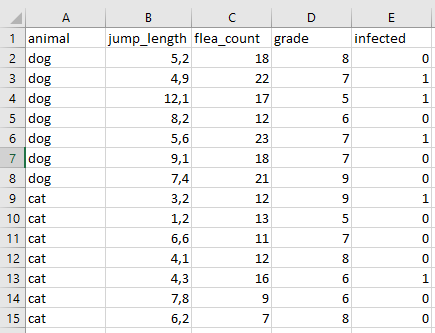
\includegraphics{./images/import_03.PNG}

}

\caption{\label{fig-imp-long}Beispiel für eine Exceldatentabelle in Long
Format.}

\end{figure}

Im Folgenden sehen wir einmal wie die Funktion \texttt{gather()} das
\texttt{tibble()} in Wide Format in ein \texttt{tibble()} in Long Format
umwandelt. Wir müssen dafür noch die Spalte benennen mit der Option
\texttt{key\ =} in die die Namen der Spalten aus dem Wide Format
geschrieben werden sowie den Spaltennamen für die eigentlichen Messwerte
mit der Option \texttt{value\ =}.

\begin{Shaded}
\begin{Highlighting}[]
\NormalTok{jump\_tbl }\OtherTok{\textless{}{-}} \FunctionTok{tibble}\NormalTok{(}\AttributeTok{dog =} \FunctionTok{c}\NormalTok{(}\FloatTok{5.2}\NormalTok{, }\FloatTok{4.9}\NormalTok{, }\FloatTok{12.1}\NormalTok{, }\FloatTok{8.2}\NormalTok{, }\FloatTok{5.6}\NormalTok{, }\FloatTok{9.1}\NormalTok{, }\FloatTok{7.4}\NormalTok{),}
                   \AttributeTok{cat =} \FunctionTok{c}\NormalTok{(}\FloatTok{10.1}\NormalTok{, }\FloatTok{9.4}\NormalTok{, }\FloatTok{11.8}\NormalTok{, }\FloatTok{6.7}\NormalTok{, }\FloatTok{8.2}\NormalTok{, }\FloatTok{9.1}\NormalTok{, }\FloatTok{7.1}\NormalTok{)) }\SpecialCharTok{\%\textgreater{}\%}
  \FunctionTok{gather}\NormalTok{(}\AttributeTok{key =} \StringTok{"animal"}\NormalTok{, }\AttributeTok{value =} \StringTok{"jump\_length"}\NormalTok{)}
\NormalTok{jump\_tbl}
\end{Highlighting}
\end{Shaded}

\begin{verbatim}
# A tibble: 14 x 2
   animal jump_length
   <chr>        <dbl>
 1 dog            5.2
 2 dog            4.9
 3 dog           12.1
 4 dog            8.2
 5 dog            5.6
 6 dog            9.1
 7 dog            7.4
 8 cat           10.1
 9 cat            9.4
10 cat           11.8
11 cat            6.7
12 cat            8.2
13 cat            9.1
14 cat            7.1
\end{verbatim}

Wir sehen, dass ein Long Format viel mehr Paltz benötigt. Das ist aber
in R kein Problem. Wir sehen die Daten kaum sondern nutzen Funktionen
wie \texttt{ggplot()} um die Daten zu visualisieren. Wichtig ist, dass
du die Daten in Excel sauber abgelegt hast.

Im Folgenden schauen wir uns noch komplexere Daten in
Tabelle~\ref{tbl-imp-complex-long} an. Das Datenbeispiel ist im Wide
Format mit einem Behandlungsfaktor \texttt{treatment} einem
Clusterfaktor \texttt{block} sowie mehreren Messwiederholungen zu
unterschiedichen Zeitpunkten \texttt{t\_1} bis \texttt{t\_6} angelegt.

\hypertarget{tbl-imp-complex-long}{}
\begin{longtable}[]{@{}cccccccc@{}}
\caption{\label{tbl-imp-complex-long}Komplexeres Datenbeispiel im Wide
Format mit einem Behandlungsfaktor \texttt{treatment} einem
Clusterfaktor \texttt{block} sowie mehreren Messwiederholungen zu
unterschiedichen Zeitpunkten \texttt{t\_1} bis
\texttt{t\_6}.}\tabularnewline
\toprule()
treatment & block & t\_1 & t\_2 & t\_3 & t\_4 & t\_5 & t\_6 \\
\midrule()
\endfirsthead
\toprule()
treatment & block & t\_1 & t\_2 & t\_3 & t\_4 & t\_5 & t\_6 \\
\midrule()
\endhead
A & 1 & 12.54 & 16.90 & 17.72 & 14.72 & 17.28 & 18.99 \\
A & 2 & 14.18 & 17.51 & 17.60 & 14.27 & 17.70 & 18.64 \\
A & 3 & 13.63 & 19.28 & 17.77 & 13.42 & 20.87 & 18.25 \\
A & 4 & 14.63 & 13.44 & 16.81 & 16.05 & 17.80 & 19.15 \\
B & 1 & 15.92 & 15.75 & 12.50 & 15.95 & 15.40 & 20.47 \\
B & 2 & 15.41 & 15.13 & 16.04 & 13.45 & 16.29 & 18.18 \\
B & 3 & 14.26 & 16.41 & 17.73 & 17.71 & 18.49 & 16.91 \\
B & 4 & 17.57 & 15.52 & 17.37 & 16.94 & 18.02 & 18.69 \\
C & 1 & 16.64 & 19.33 & 17.23 & 17.80 & 22.37 & 21.54 \\
C & 2 & 16.05 & 16.19 & 15.81 & 16.66 & 18.79 & 12.98 \\
C & 3 & 14.87 & 17.08 & 12.12 & 15.53 & 16.61 & 20.36 \\
C & 4 & 14.75 & 13.04 & 17.48 & 19.01 & 20.73 & 19.34 \\
D & 1 & 13.11 & 14.86 & 17.50 & 16.56 & 17.35 & 16.15 \\
D & 2 & 17.72 & 15.08 & 17.86 & 13.83 & 20.43 & 12.77 \\
D & 3 & 18.60 & 15.08 & 16.12 & 17.32 & 16.54 & 17.37 \\
D & 4 & 12.44 & 16.64 & 19.34 & 19.00 & 18.93 & 19.87 \\
\bottomrule()
\end{longtable}

Im Folgenden Codeblock sehen wir, wie die Funktion \texttt{gather()} die
Daten in Tabelle Tabelle~\ref{tbl-imp-complex-long} in ein Long Format
umwandelt. Die Funktion fasst die Messwiederholungen der Spalten
\texttt{t\_1} bis \texttt{t\_6} zusammen, in dem die Werte alle in der
Spalte \texttt{drymatter} untereinander geklebt werden. Die Spalten
\texttt{treatment} und \texttt{block} werden dann sechs Mal wiederholt
untereinander geklebt.

\begin{Shaded}
\begin{Highlighting}[]
\NormalTok{data\_tbl }\SpecialCharTok{\%\textgreater{}\%} 
  \FunctionTok{gather}\NormalTok{(}\AttributeTok{key =} \StringTok{"time\_point"}\NormalTok{, }\AttributeTok{value =} \StringTok{"drymatter"}\NormalTok{, t\_1}\SpecialCharTok{:}\NormalTok{t\_6) }\SpecialCharTok{\%\textgreater{}\%} 
  \FunctionTok{arrange}\NormalTok{(treatment, block)}
\end{Highlighting}
\end{Shaded}

\begin{verbatim}
# A tibble: 96 x 4
   treatment block time_point drymatter
   <fct>     <int> <chr>          <dbl>
 1 A             1 t_1             12.5
 2 A             1 t_2             16.9
 3 A             1 t_3             17.7
 4 A             1 t_4             14.7
 5 A             1 t_5             17.3
 6 A             1 t_6             19.0
 7 A             2 t_1             14.2
 8 A             2 t_2             17.5
 9 A             2 t_3             17.6
10 A             2 t_4             14.3
# ... with 86 more rows
\end{verbatim}

\hypertarget{importieren-mit-rstudio}{%
\section{Importieren mit RStudio}\label{importieren-mit-rstudio}}

Wir können das RStudio nutzen um Daten mit Point-and-Klick rein zuladen
und dann den Code wieder in den Editor kopieren. Im Prinzip ist dieser
Weg der einfachste um einmal zu sehen, wie ein pfad funktioniert und der
Code lautet. Später benötigt man diese `Krücke' nicht mehr. Wir nutzen
dann direkt den Pfad zu der Datei. Abbildung~\ref{fig-imp-01} zeigt
einen Ausschnitt, wo wir im RStudio die \emph{Import Dataset}
Funktionalität finden.

\begin{figure}

{\centering 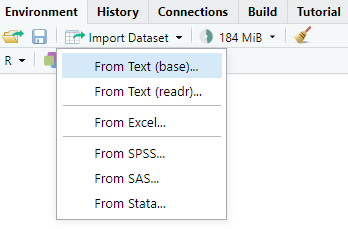
\includegraphics[width=3.125in,height=\textheight]{./images/import_01.PNG}

}

\caption{\label{fig-imp-01}Auf den Reiter \emph{Einviroment} klicken und
dann \emph{Import Dataset}. In der deutschen version vom RStudio mögen
die Begriffe leicht anders sein.}

\end{figure}

\begin{tcolorbox}[enhanced jigsaw, coltitle=black, titlerule=0mm, bottomrule=.15mm, opacityback=0, opacitybacktitle=0.6, leftrule=.75mm, title=\textcolor{quarto-callout-tip-color}{\faLightbulb}\hspace{0.5em}{Importieren mit RStudio als Video}, toprule=.15mm, bottomtitle=1mm, toptitle=1mm, left=2mm, breakable, arc=.35mm, colback=white, rightrule=.15mm, colbacktitle=quarto-callout-tip-color!10!white, colframe=quarto-callout-tip-color-frame]
Du findest auf YouTube \href{https://youtu.be/tdRWkBcGAzk}{Einführung in
R - Teil 21.0 - Daten importieren mit RStudio - Point and Klick} als
Video. Point and Klick ist als Video einfacher nachzuvollziehen als
Screenshots in einem Fließtext.
\end{tcolorbox}

\hypertarget{sec-pfad}{%
\section{Importieren per Pfad}\label{sec-pfad}}

In Abbildung~\ref{fig-imp-02} können wir sehen wie wir den Pfad zu
unserer Excel Datei \texttt{flea\_dog\_cat.xlsx} finden. Natürlich
kannst du den Pfad auch anders herausfinden bzw. aus dem Explorer oder
Finder kopieren.

\begin{figure}

{\centering 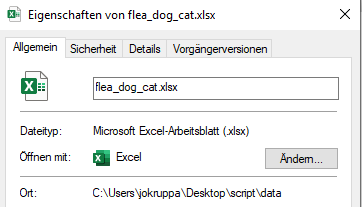
\includegraphics[width=3.64583in,height=\textheight]{./images/import_02.PNG}

}

\caption{\label{fig-imp-02}Durch den Rechts-Klick auf die Eigenschaften
einer Datei kann man sich den Pfad zur Datei anzeigen lassen.
\textbf{Achtung!} Unter Windows muss der Slash \texttt{\textbackslash{}}
noch in den Backslash \texttt{/} gedreht werden.}

\end{figure}

Nachdem wir den Pfad gefunden haben, können wir den Pfad in die Funktion
\texttt{read\_excel()} kopieren und die Datei in das Objekt
\texttt{data\_tbl} einlesen. Ja, es wird nichts in der R Console
ausgegeben, da sich die Daten jetzt in dem Object \texttt{data\_tbl}
befinden.

\begin{Shaded}
\begin{Highlighting}[]
\DocumentationTok{\#\# Ganzer Pfad zur Datei flea\_dog\_cat.xlsx}
\NormalTok{data\_tbl }\OtherTok{\textless{}{-}} \FunctionTok{read\_excel}\NormalTok{(}\StringTok{"data/flea\_dog\_cat.xlsx"}\NormalTok{)}
\end{Highlighting}
\end{Shaded}

\begin{tcolorbox}[enhanced jigsaw, coltitle=black, titlerule=0mm, bottomrule=.15mm, opacityback=0, opacitybacktitle=0.6, leftrule=.75mm, title=\textcolor{quarto-callout-important-color}{\faExclamation}\hspace{0.5em}{Unterschied zwischen \texttt{\textbackslash{}} in Windows und \texttt{/}
in R}, toprule=.15mm, bottomtitle=1mm, toptitle=1mm, left=2mm, breakable, arc=.35mm, colback=white, rightrule=.15mm, colbacktitle=quarto-callout-important-color!10!white, colframe=quarto-callout-important-color-frame]
Achte einmal auf den Slash im Pfad in R und einem im Pfsd in Windows.
Einmal ist es der Slash \texttt{\textbackslash{}} im Dateipfad und
einmal der Backslash \texttt{/}. Das ist sehr ärgerlich, aber dieses
Problem geht zurück in die 80'ziger. Bill hat entschieden für sein
Windows \texttt{/} zu nutzen und Steve (und Unix) eben \texttt{/}. Und
mit dieser Entscheidung müssen wir jetzt leben\ldots{}
\end{tcolorbox}

\hypertarget{sec-umlaute}{%
\section{Auf ein englisches Wort in Dateien}\label{sec-umlaute}}

Ein großes Problem in Datein sind Umlaute (ä,ö,ü) oder aber andere
(Sonder)zeichen (ß, ?, oder \#). Als dies sollte vermieden werden. Eine
gute Datei für R beinhaltet nur \emph{ganze} Wörter, Zahlen oder aber
leere Felder. Ein leeres Feld ist ein fehlender Wert.
Abbildung~\ref{fig-imp-03} zeigt eine gute Exceldatentablle. Wir
schreiben \texttt{jump\_length} mit Unterstrich um den Namen besser zu
lesen zu können. Sonst ist auch alles in Englisch geschrieben. Wir
vermeiden durch die neglische Schreibweise \emph{aus versehen} einen
Umlaut oder anderweitig problematische Zeichen zu verwenden. Später
können wir alles noch für Abbildungen anpassen.

\begin{figure}

{\centering 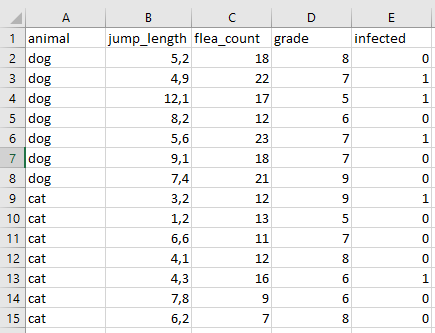
\includegraphics{./images/import_03.PNG}

}

\caption{\label{fig-imp-03}Beispiel für eine gute (Excel)Datentabelle.
Keine Umlaute sind vorhanden und die Spaltennamen haben keine
Leerzeichen oder Sonderzeichen.}

\end{figure}

\hypertarget{sec-spalten}{%
\section{Spaltennamen in der (Excel)-Datei}\label{sec-spalten}}

Die Funktion \texttt{clean\_names()} aus dem R Paket \texttt{janitor}
erlaubt es die Spaltennamen einer eingelesenen Datei in eine für R gute
Form zu bringen.

\begin{itemize}
\tightlist
\item
  Keine Leerzeichen in den Spaltennamen.
\item
  Alle Spaltennamen sind klein geschrieben.
\end{itemize}

\begin{Shaded}
\begin{Highlighting}[]
\NormalTok{data\_tbl }\SpecialCharTok{\%\textgreater{}\%} 
  \FunctionTok{clean\_names}\NormalTok{()}
\end{Highlighting}
\end{Shaded}

\begin{verbatim}
# A tibble: 14 x 5
   animal jump_length flea_count grade infected
   <chr>        <dbl>      <dbl> <dbl>    <dbl>
 1 dog            5.7         18     8        0
 2 dog            8.9         22     8        1
 3 dog           11.8         17     6        1
 4 dog            8.2         12     8        0
 5 dog            5.6         23     7        1
 6 dog            9.1         18     7        0
 7 dog            7.6         21     9        0
 8 cat            3.2         12     7        1
 9 cat            2.2         13     5        0
10 cat            5.4         11     7        0
11 cat            4.1         12     6        0
12 cat            4.3         16     6        1
13 cat            7.9          9     6        0
14 cat            6.1          7     5        0
\end{verbatim}

\hypertarget{sec-dplyr}{%
\chapter{Daten bearbeiten}\label{sec-dplyr}}

\emph{Version vom September 14, 2022 um 08:46:32}

Wir haben in dem vorherigen Kapitel Daten eingelesen. Jetzt wollen wir
die Daten aufräumen (eng. \emph{tidy}). Es ist notwendig, dass wir die
Daten so aufarbeiten, dass R damit umgehen kann. Insbesondere das
Erstellen von Faktoren ist wichtig, wenn die Spalte ein Faktor ist. R
muss wissen was für Eigenschaften eine Spalte hat. Sonst funktionieren
spätere Anwendungen in R nicht richtig oder geben einen Fehler wieder.

Es gibt zwei Möglichkeiten wie du mit deinen Daten umgehst:

\begin{enumerate}
\def\labelenumi{\arabic{enumi})}
\tightlist
\item
  Du änderst all deine Daten in Excel. Das mag bei einem kleinen
  Datensatz gut funktionieren. Dann musst du dich nicht mit dem
  \emph{Programmieren} beschäftigen.
\item
  Du willst lernen die Daten auch in R zu verändern. Dann hilft dir
  dieses Kapitel. Auch in den folgenden Kapiteln werde ich immer wieder
  Funktionen wie \texttt{select()}, \texttt{filter()} und
  \texttt{mutate()}nutzen. Dann kannst du hier nochmal schauen, was die
  Funktionen machen.
\end{enumerate}

Im Folgenden wollen wir den Datensatz \texttt{data\_tbl} in R
bearbeiten. Das heißt wir wollen Spalten auswählen mit \texttt{select()}
oder Zeilen auswählen mit \texttt{filter()}. Schlussendlich wollen wir
auch die Eigenschaften von Spalten mit der Funktion \texttt{mutate}
ändern. Wir laden also den Datensatz \texttt{flea\_dog\_cat.xlsx} einmal
in R.

\begin{Shaded}
\begin{Highlighting}[]
\NormalTok{data\_tbl }\OtherTok{\textless{}{-}} \FunctionTok{read\_excel}\NormalTok{(}\StringTok{"data/flea\_dog\_cat\_fox.xlsx"}\NormalTok{)}
\end{Highlighting}
\end{Shaded}

Es ergibt sich folgende Tabelle~\ref{tbl-dog-cat-dplyr}, die wir schon
aus vorherigen Kapiteln kennen.

\hypertarget{tbl-dog-cat-dplyr}{}
\begin{longtable}[]{@{}ccccc@{}}
\caption{\label{tbl-dog-cat-dplyr}Tabelle der Sprunglängen {[}cm{]},
Anzahl an Flöhen, Boniturnote sowie der Infektionsstatus von Hunden,
Katzen und Füchsen.}\tabularnewline
\toprule()
animal & jump\_length & flea\_count & grade & infected \\
\midrule()
\endfirsthead
\toprule()
animal & jump\_length & flea\_count & grade & infected \\
\midrule()
\endhead
dog & 5.7 & 18 & 8 & 0 \\
dog & 8.9 & 22 & 8 & 1 \\
dog & 11.8 & 17 & 6 & 1 \\
dog & 8.2 & 12 & 8 & 0 \\
dog & 5.6 & 23 & 7 & 1 \\
dog & 9.1 & 18 & 7 & 0 \\
dog & 7.6 & 21 & 9 & 0 \\
cat & 3.2 & 12 & 7 & 1 \\
cat & 2.2 & 13 & 5 & 0 \\
cat & 5.4 & 11 & 7 & 0 \\
cat & 4.1 & 12 & 6 & 0 \\
cat & 4.3 & 16 & 6 & 1 \\
cat & 7.9 & 9 & 6 & 0 \\
cat & 6.1 & 7 & 5 & 0 \\
fox & 7.7 & 21 & 5 & 1 \\
fox & 8.1 & 25 & 4 & 1 \\
fox & 9.1 & 31 & 4 & 1 \\
fox & 9.7 & 12 & 5 & 1 \\
fox & 10.6 & 28 & 4 & 0 \\
fox & 8.6 & 18 & 4 & 1 \\
fox & 10.3 & 19 & 3 & 0 \\
\bottomrule()
\end{longtable}

\hypertarget{genutzte-r-pakete-fuxfcr-das-kapitel-1}{%
\section{Genutzte R Pakete für das
Kapitel}\label{genutzte-r-pakete-fuxfcr-das-kapitel-1}}

Wir wollen folgende R Pakete in diesem Kapitel nutzen.

\begin{Shaded}
\begin{Highlighting}[]
\NormalTok{pacman}\SpecialCharTok{::}\FunctionTok{p\_load}\NormalTok{(tidyverse, readxl, magrittr, janitor)}
\end{Highlighting}
\end{Shaded}

Am Ende des Kapitels findest du nochmal den gesamten R Code in einem
Rutsch zum selber durchführen oder aber kopieren.

\hypertarget{spalten-wuxe4hlen-mit-select}{%
\section{\texorpdfstring{Spalten wählen mit
\texttt{select()}}{Spalten wählen mit select()}}\label{spalten-wuxe4hlen-mit-select}}

\begin{tcolorbox}[enhanced jigsaw, coltitle=black, titlerule=0mm, bottomrule=.15mm, opacityback=0, opacitybacktitle=0.6, leftrule=.75mm, title=\textcolor{quarto-callout-tip-color}{\faLightbulb}\hspace{0.5em}{YouTube - Spalten auswählen mit select()}, toprule=.15mm, bottomtitle=1mm, toptitle=1mm, left=2mm, breakable, arc=.35mm, colback=white, rightrule=.15mm, colbacktitle=quarto-callout-tip-color!10!white, colframe=quarto-callout-tip-color-frame]
Du findest auf YouTube \href{https://youtu.be/oV_7A2nMIrM}{Einführung in
R - Teil 12 - Spalten auswählen mit select()} als Video zum nochmal
anschauen.
\end{tcolorbox}

{\marginnote{\begin{footnotesize}Wir nutzen die Funktion
\texttt{select()}um Spalten zu wählen.\end{footnotesize}}}

Der Datensatz, den wir im Experiment erschaffen, ist meist riesig. Jetzt
könnten wir natürlich eine Exceltabelle mit unterschiedlichen Sheets
bzw. Reitern erstellen oder aber die \emph{Spalten} die wir brauchen in
R selektieren. Wir nutzen die Funktion \texttt{select()}um Spalten zu
wählen. Im folgenden Codeblock wählen wir die Spalten \texttt{animal},
\texttt{jump\_length} und \texttt{flea\_count}.

\begin{Shaded}
\begin{Highlighting}[]
\NormalTok{data\_tbl }\SpecialCharTok{\%\textgreater{}\%} 
  \FunctionTok{select}\NormalTok{(animal, jump\_length, flea\_count)}
\end{Highlighting}
\end{Shaded}

\begin{verbatim}
# A tibble: 21 x 3
   animal jump_length flea_count
   <chr>        <dbl>      <dbl>
 1 dog            5.7         18
 2 dog            8.9         22
 3 dog           11.8         17
 4 dog            8.2         12
 5 dog            5.6         23
 6 dog            9.1         18
 7 dog            7.6         21
 8 cat            3.2         12
 9 cat            2.2         13
10 cat            5.4         11
# ... with 11 more rows
\end{verbatim}

Wir können die Spalten beim selektieren auch umbenennen und in eine
andere Reihenfolge bringen.

\begin{Shaded}
\begin{Highlighting}[]
\NormalTok{data\_tbl }\SpecialCharTok{\%\textgreater{}\%} 
  \FunctionTok{select}\NormalTok{(}\AttributeTok{Sprungweite =}\NormalTok{ jump\_length, flea\_count, animal)}
\end{Highlighting}
\end{Shaded}

\begin{verbatim}
# A tibble: 21 x 3
   Sprungweite flea_count animal
         <dbl>      <dbl> <chr> 
 1         5.7         18 dog   
 2         8.9         22 dog   
 3        11.8         17 dog   
 4         8.2         12 dog   
 5         5.6         23 dog   
 6         9.1         18 dog   
 7         7.6         21 dog   
 8         3.2         12 cat   
 9         2.2         13 cat   
10         5.4         11 cat   
# ... with 11 more rows
\end{verbatim}

Du findest auf der englischen
\href{https://dplyr.tidyverse.org/reference/select.html}{Hilfeseite für
select()} noch weitere Beispiele für die Nutzung.

\hypertarget{zeilen-wuxe4hlen-mit-filter}{%
\section{\texorpdfstring{Zeilen wählen mit
\texttt{filter()}}{Zeilen wählen mit filter()}}\label{zeilen-wuxe4hlen-mit-filter}}

\begin{tcolorbox}[enhanced jigsaw, coltitle=black, titlerule=0mm, bottomrule=.15mm, opacityback=0, opacitybacktitle=0.6, leftrule=.75mm, title=\textcolor{quarto-callout-tip-color}{\faLightbulb}\hspace{0.5em}{YouTube - Zeilen auswählen mit filter()}, toprule=.15mm, bottomtitle=1mm, toptitle=1mm, left=2mm, breakable, arc=.35mm, colback=white, rightrule=.15mm, colbacktitle=quarto-callout-tip-color!10!white, colframe=quarto-callout-tip-color-frame]
Du findest auf YouTube \href{https://youtu.be/Pw_KnGWZjpM}{Einführung in
R - Teil 13 - Zeilen auswählen mit filter()} als Video zum nochmal
anschauen.
\end{tcolorbox}

{\marginnote{\begin{footnotesize}Wir nutzen die Funktion
\texttt{filter()} um Zeilen nach Kriterien zu
wählen.\end{footnotesize}}}

Während wir die Auswahl an Spalten gut und gerne auch in Excel
durchführen können, so ist dies bei der Auswahl der Zeilen nicht so
einfach. Wir können in R hier auf die Funktion \texttt{filter()}
zurückgreifen. Wir nutzen die Funktion \texttt{filter()} um Zeilen nach
Kriterien zu wählen.

Im folgenden Codeblock wählen wir die Zeilen aus in denen die Worte
\texttt{dog} und \texttt{fox} stehen. Wir nutzen dazu den Operator
\texttt{\%in\%} um auszudrücken, dass wir alle Einträge in der Spalte
\texttt{animal} wollen die in dem Vektor \texttt{c("dog",\ "fox")}
beschrieben sind.

\begin{Shaded}
\begin{Highlighting}[]
\NormalTok{data\_tbl }\SpecialCharTok{\%\textgreater{}\%} 
  \FunctionTok{filter}\NormalTok{(animal }\SpecialCharTok{\%in\%} \FunctionTok{c}\NormalTok{(}\StringTok{"dog"}\NormalTok{, }\StringTok{"fox"}\NormalTok{))}
\end{Highlighting}
\end{Shaded}

\begin{verbatim}
# A tibble: 14 x 5
   animal jump_length flea_count grade infected
   <chr>        <dbl>      <dbl> <dbl>    <dbl>
 1 dog            5.7         18     8        0
 2 dog            8.9         22     8        1
 3 dog           11.8         17     6        1
 4 dog            8.2         12     8        0
 5 dog            5.6         23     7        1
 6 dog            9.1         18     7        0
 7 dog            7.6         21     9        0
 8 fox            7.7         21     5        1
 9 fox            8.1         25     4        1
10 fox            9.1         31     4        1
11 fox            9.7         12     5        1
12 fox           10.6         28     4        0
13 fox            8.6         18     4        1
14 fox           10.3         19     3        0
\end{verbatim}

Es stehen dir Folgende logische Operatoren zu Verfügung wie in
Tabelle~\ref{tbl-logical-operators} gezeigt. Am Anfang ist es immer
etwas schwer sich in den logischen Operatoren zurechtzufinden. Daher
kann ich dir nur den Tipp geben einmal die Operatoren selber
auszuprobieren und zu schauen, was du da so rausfilterst.

\hypertarget{tbl-logical-operators}{}
\begin{longtable}[]{@{}
  >{\raggedright\arraybackslash}p{(\columnwidth - 2\tabcolsep) * \real{0.2927}}
  >{\raggedright\arraybackslash}p{(\columnwidth - 2\tabcolsep) * \real{0.7073}}@{}}
\caption{\label{tbl-logical-operators}Logische Opertairen und R und
deren Beschreibung}\tabularnewline
\toprule()
\begin{minipage}[b]{\linewidth}\raggedright
\textbf{Logischer Operator}
\end{minipage} & \begin{minipage}[b]{\linewidth}\raggedright
\textbf{Beschreibung}
\end{minipage} \\
\midrule()
\endfirsthead
\toprule()
\begin{minipage}[b]{\linewidth}\raggedright
\textbf{Logischer Operator}
\end{minipage} & \begin{minipage}[b]{\linewidth}\raggedright
\textbf{Beschreibung}
\end{minipage} \\
\midrule()
\endhead
\textbf{\textless{}} & kleiner als (eng. \emph{less than}) \\
\textbf{\textless=} & kleiner als oder gleich (eng. \emph{less than or
equal to}) \\
\textbf{\textgreater{}} & größer als (eng. \emph{greater than}) \\
\textbf{\textgreater=} & größer als oder gleich (eng. \emph{greater than
or equal to}) \\
\textbf{==} & exact gleich (eng. \emph{exactly equal to}) \\
\textbf{!=} & nicht gleich (eng. \emph{not equal to}) \\
\textbf{!x} & nicht (eng. \emph{not x}) \\
\textbf{x \textbar{} y} & oder (eng. \emph{x or y}) \\
\textbf{x \& y} & und (eng. \emph{x and y}) \\
\bottomrule()
\end{longtable}

Hier ein paar Beispiele. Probiere gerne auch mal Operatoren selber aus.
Im folgenden Codeblock wollen wir nur die Zeilen haben, die eine Anzahl
an Flöhen größer von 15 haben.

\begin{Shaded}
\begin{Highlighting}[]
\NormalTok{data\_tbl }\SpecialCharTok{\%\textgreater{}\%} 
  \FunctionTok{filter}\NormalTok{(flea\_count }\SpecialCharTok{\textgreater{}} \DecValTok{15}\NormalTok{)}
\end{Highlighting}
\end{Shaded}

\begin{verbatim}
# A tibble: 13 x 5
   animal jump_length flea_count grade infected
   <chr>        <dbl>      <dbl> <dbl>    <dbl>
 1 dog            5.7         18     8        0
 2 dog            8.9         22     8        1
 3 dog           11.8         17     6        1
 4 dog            5.6         23     7        1
 5 dog            9.1         18     7        0
 6 dog            7.6         21     9        0
 7 cat            4.3         16     6        1
 8 fox            7.7         21     5        1
 9 fox            8.1         25     4        1
10 fox            9.1         31     4        1
11 fox           10.6         28     4        0
12 fox            8.6         18     4        1
13 fox           10.3         19     3        0
\end{verbatim}

Wir wollen nur die infizierten Tiere haben.

\begin{Shaded}
\begin{Highlighting}[]
\NormalTok{data\_tbl }\SpecialCharTok{\%\textgreater{}\%} 
  \FunctionTok{filter}\NormalTok{(infected }\SpecialCharTok{==} \ConstantTok{TRUE}\NormalTok{)}
\end{Highlighting}
\end{Shaded}

\begin{verbatim}
# A tibble: 10 x 5
   animal jump_length flea_count grade infected
   <chr>        <dbl>      <dbl> <dbl>    <dbl>
 1 dog            8.9         22     8        1
 2 dog           11.8         17     6        1
 3 dog            5.6         23     7        1
 4 cat            3.2         12     7        1
 5 cat            4.3         16     6        1
 6 fox            7.7         21     5        1
 7 fox            8.1         25     4        1
 8 fox            9.1         31     4        1
 9 fox            9.7         12     5        1
10 fox            8.6         18     4        1
\end{verbatim}

Wir wollen nur die infizierten Tiere haben UND die Tiere mit einer
Flohanzahl größer als 20.

\begin{Shaded}
\begin{Highlighting}[]
\NormalTok{data\_tbl }\SpecialCharTok{\%\textgreater{}\%} 
  \FunctionTok{filter}\NormalTok{(infected }\SpecialCharTok{==} \ConstantTok{TRUE} \SpecialCharTok{\&}\NormalTok{ flea\_count }\SpecialCharTok{\textgreater{}} \DecValTok{20}\NormalTok{)}
\end{Highlighting}
\end{Shaded}

\begin{verbatim}
# A tibble: 5 x 5
  animal jump_length flea_count grade infected
  <chr>        <dbl>      <dbl> <dbl>    <dbl>
1 dog            8.9         22     8        1
2 dog            5.6         23     7        1
3 fox            7.7         21     5        1
4 fox            8.1         25     4        1
5 fox            9.1         31     4        1
\end{verbatim}

Du findest auf der englischen
\href{https://dplyr.tidyverse.org/reference/filter.html\%3E}{Hilfeseite
für filter()} noch weitere Beispiele für die Nutzung.

\hypertarget{spalten-uxe4ndern-mit-mutate}{%
\section{\texorpdfstring{Spalten ändern mit
\texttt{mutate()}}{Spalten ändern mit mutate()}}\label{spalten-uxe4ndern-mit-mutate}}

\begin{tcolorbox}[enhanced jigsaw, coltitle=black, titlerule=0mm, bottomrule=.15mm, opacityback=0, opacitybacktitle=0.6, leftrule=.75mm, title=\textcolor{quarto-callout-tip-color}{\faLightbulb}\hspace{0.5em}{YouTube - Eigenschaften von Variablen ändern mit mutate()}, toprule=.15mm, bottomtitle=1mm, toptitle=1mm, left=2mm, breakable, arc=.35mm, colback=white, rightrule=.15mm, colbacktitle=quarto-callout-tip-color!10!white, colframe=quarto-callout-tip-color-frame]
Du findest auf YouTube \href{https://youtu.be/P6eum3wy9Ek}{Einführung in
R - Teil 14 - Eigenschaften von Variablen ändern mit mutate()} als Video
zum nochmal anschauen.
\end{tcolorbox}

\marginnote{\begin{footnotesize}

Wir nutzen die Funktion \texttt{mutate()} um die Eigenschaften von
Spalten daher Variablen zu ändern.

Die Reihenfolge der Funktionen ist wichtig um unliebsame Effekte zu
vermeiden.

\begin{enumerate}
\def\labelenumi{\arabic{enumi})}
\tightlist
\item
  Erst wählen wir die Spalten mit \texttt{select()}
\item
  Dann filtern wir die Zeilen mit \texttt{filter()}
\item
  Abschließend ändern wir die Eigenschaften der Spalten mit
  \texttt{mutate()}
\end{enumerate}

\end{footnotesize}}

Nachdem wir die Spalten mit \texttt{select()} udn eventuell die Zeieln
mit \texttt{filter()} gewählt haben. müssen wir jetzt noch die
Eigenschaften der Spalten ändern. Das Ändern müssen wir nicht immer tun,
aber häufig müssen wir noch einen Faktor erschaffen. Wir nutzen noch die
Funktion \texttt{pull()} um uns die Spalte \texttt{animal} aus dem
Datensatz zu ziehen. Nur so sehen wir die vollen Eigenschaften des
Faktors. Später nutzen wir \texttt{pull} seltener und nur um zu
kontrollieren, was wir gemacht haben.

Im folgenden Codeblock verwandeln wir die Variable \texttt{animal} in
einen Faktor durch die Funktion \texttt{as\_factor}. Wir sehen, dass die
Level des Faktoes so sortiert sind, wie das Auftreten in der Spalte
\texttt{animal}.

\begin{Shaded}
\begin{Highlighting}[]
\NormalTok{data\_tbl }\SpecialCharTok{\%\textgreater{}\%} 
  \FunctionTok{mutate}\NormalTok{(}\AttributeTok{animal =} \FunctionTok{as\_factor}\NormalTok{(animal)) }\SpecialCharTok{\%\textgreater{}\%} 
  \FunctionTok{pull}\NormalTok{(animal)}
\end{Highlighting}
\end{Shaded}

\begin{verbatim}
 [1] dog dog dog dog dog dog dog cat cat cat cat cat cat cat fox fox fox fox fox
[20] fox fox
Levels: dog cat fox
\end{verbatim}

Wollen wir die Sortierung der Level ändern, können wir die Funktion
\texttt{factor()} nutzen. Wir ändern die Sortierung des Faktors zu
\texttt{fox}, \texttt{dog} und \texttt{cat}.

\begin{Shaded}
\begin{Highlighting}[]
\NormalTok{data\_tbl }\SpecialCharTok{\%\textgreater{}\%} 
  \FunctionTok{mutate}\NormalTok{(}\AttributeTok{animal =} \FunctionTok{factor}\NormalTok{(animal, }\AttributeTok{levels =} \FunctionTok{c}\NormalTok{(}\StringTok{"fox"}\NormalTok{, }\StringTok{"dog"}\NormalTok{, }\StringTok{"cat"}\NormalTok{))) }\SpecialCharTok{\%\textgreater{}\%} 
  \FunctionTok{pull}\NormalTok{(animal)}
\end{Highlighting}
\end{Shaded}

\begin{verbatim}
 [1] dog dog dog dog dog dog dog cat cat cat cat cat cat cat fox fox fox fox fox
[20] fox fox
Levels: fox dog cat
\end{verbatim}

Wir können auch die Namen (eng. \emph{labels}) der Level ändern. Hier
musst du nur aufpassen wie du die alten Labels überschreibst. Wenn ich
\emph{gleichzeitig} die Level und die Labels ändere komme ich häufig
durcheinander. Da muss du eventuell nochmal schauen, ob auch alles so
geklappt hat wie du wolltest.

\begin{Shaded}
\begin{Highlighting}[]
\NormalTok{data\_tbl }\SpecialCharTok{\%\textgreater{}\%} 
  \FunctionTok{mutate}\NormalTok{(}\AttributeTok{animal =} \FunctionTok{factor}\NormalTok{(animal, }\AttributeTok{labels =} \FunctionTok{c}\NormalTok{(}\StringTok{"Hund"}\NormalTok{, }\StringTok{"Katze"}\NormalTok{, }\StringTok{"Fuchs"}\NormalTok{))) }\SpecialCharTok{\%\textgreater{}\%} 
  \FunctionTok{pull}\NormalTok{(animal)}
\end{Highlighting}
\end{Shaded}

\begin{verbatim}
 [1] Katze Katze Katze Katze Katze Katze Katze Hund  Hund  Hund  Hund  Hund 
[13] Hund  Hund  Fuchs Fuchs Fuchs Fuchs Fuchs Fuchs Fuchs
Levels: Hund Katze Fuchs
\end{verbatim}

Du findest auf der englischen
\href{https://dplyr.tidyverse.org/reference/mutate.html}{Hilfeseite für
mutate()} noch weitere Beispiele für die Nutzung. Insbesondere die
Nutzung von \texttt{mutate()} über mehrere Spalten gleichzeitig erlaubt
sehr effiezientes Programmieren. Aber das ist für den Anfang etwas viel.

\begin{tcolorbox}[enhanced jigsaw, coltitle=black, titlerule=0mm, bottomrule=.15mm, opacityback=0, opacitybacktitle=0.6, leftrule=.75mm, title=\textcolor{quarto-callout-note-color}{\faInfo}\hspace{0.5em}{Die Funktionen select(), filter() und mutate() in R}, toprule=.15mm, bottomtitle=1mm, toptitle=1mm, left=2mm, breakable, arc=.35mm, colback=white, rightrule=.15mm, colbacktitle=quarto-callout-note-color!10!white, colframe=quarto-callout-note-color-frame]
Bitte schaue dir auch die Hilfeseiten der Funktionen an. In diesem
Skript kann ich nicht alle Funktionalitäten der Funktionen zeigen. Oder
du kommst in das R Tutorium welches ich anbiete und fragst dort nach den
Möglichkeiten Daten in R zu verändern.
\end{tcolorbox}

\hypertarget{gruppieren-mit-group_by}{%
\section{\texorpdfstring{Gruppieren mit
\texttt{group\_by()}}{Gruppieren mit group\_by()}}\label{gruppieren-mit-group_by}}

Sobald wir einen Faktor erschaffen haben, können wir die Daten in R auch
nach dem Faktor \emph{gruppieren}. Das heißt wir nutzen die Funktion
\texttt{group\_by()} um R mitzuteilen, dass nun folgende Funktionen
\emph{getrennt} für die einzelen Gruppen erfolgen sollen. Im folgenden
Codeblock siehst du die Anwendung.

\begin{Shaded}
\begin{Highlighting}[]
\NormalTok{data\_tbl }\SpecialCharTok{\%\textgreater{}\%} 
  \FunctionTok{mutate}\NormalTok{(}\AttributeTok{animal =} \FunctionTok{as\_factor}\NormalTok{(animal)) }\SpecialCharTok{\%\textgreater{}\%} 
  \FunctionTok{group\_by}\NormalTok{(animal)}
\end{Highlighting}
\end{Shaded}

\begin{verbatim}
# A tibble: 21 x 5
# Groups:   animal [3]
   animal jump_length flea_count grade infected
   <fct>        <dbl>      <dbl> <dbl>    <dbl>
 1 dog            5.7         18     8        0
 2 dog            8.9         22     8        1
 3 dog           11.8         17     6        1
 4 dog            8.2         12     8        0
 5 dog            5.6         23     7        1
 6 dog            9.1         18     7        0
 7 dog            7.6         21     9        0
 8 cat            3.2         12     7        1
 9 cat            2.2         13     5        0
10 cat            5.4         11     7        0
# ... with 11 more rows
\end{verbatim}

Auf den ersten Blick ändert sich nicht viel. Es entsteht aber die Zeile
\texttt{\#\ Groups:\ animal\ {[}3{]}}. Wir wissen nun, dass wir nach der
Variable \texttt{animal} mit drei Gruppen die Datentabelle gruppiert
haben. Die Anwendung siehst du in Kapitel~\ref{sec-desc-group-by} bei
der Berechung von deskriptiven Maßzahlen.

\hypertarget{mehr-informationen-durch-glimpse-und-str}{%
\section{\texorpdfstring{Mehr Informationen durch \texttt{glimpse()} und
\texttt{str()}}{Mehr Informationen durch glimpse() und str()}}\label{mehr-informationen-durch-glimpse-und-str}}

Am Ende noch zwei Funktionen zur Kontrolle, was wir hier eigentlich
gerade tun. Mit der Funktion \texttt{glimpse()} können wir uns einen
Einblick in die Daten geben lassen. Wir sehen dann nochmal kurz und
knapp wieviel Zeieln und Spalten wir haben und welche Inhalte in den
Spalten stehen. Die gleichen Informationen erhalten wir auch durch die
Funktion \texttt{str()}. Die Funktion \texttt{str()}geht aber noch einen
Schritt weiter und nennt uns auch Informationen zu dem Objekt. Daher wir
wissen jetzt, dass es sich beim dem Objekt \texttt{data\_tbl} um ein
\texttt{tibble()} handelt.

\begin{Shaded}
\begin{Highlighting}[]
\FunctionTok{glimpse}\NormalTok{(data\_tbl)}
\end{Highlighting}
\end{Shaded}

\begin{verbatim}
Rows: 21
Columns: 5
$ animal      <chr> "dog", "dog", "dog", "dog", "dog", "dog", "dog", "cat", "c~
$ jump_length <dbl> 5.7, 8.9, 11.8, 8.2, 5.6, 9.1, 7.6, 3.2, 2.2, 5.4, 4.1, 4.~
$ flea_count  <dbl> 18, 22, 17, 12, 23, 18, 21, 12, 13, 11, 12, 16, 9, 7, 21, ~
$ grade       <dbl> 8, 8, 6, 8, 7, 7, 9, 7, 5, 7, 6, 6, 6, 5, 5, 4, 4, 5, 4, 4~
$ infected    <dbl> 0, 1, 1, 0, 1, 0, 0, 1, 0, 0, 0, 1, 0, 0, 1, 1, 1, 1, 0, 1~
\end{verbatim}

\begin{Shaded}
\begin{Highlighting}[]
\FunctionTok{str}\NormalTok{(data\_tbl)}
\end{Highlighting}
\end{Shaded}

\begin{verbatim}
tibble [21 x 5] (S3: tbl_df/tbl/data.frame)
 $ animal     : chr [1:21] "dog" "dog" "dog" "dog" ...
 $ jump_length: num [1:21] 5.7 8.9 11.8 8.2 5.6 9.1 7.6 3.2 2.2 5.4 ...
 $ flea_count : num [1:21] 18 22 17 12 23 18 21 12 13 11 ...
 $ grade      : num [1:21] 8 8 6 8 7 7 9 7 5 7 ...
 $ infected   : num [1:21] 0 1 1 0 1 0 0 1 0 0 ...
\end{verbatim}

\part{Explorative Datenanalyse}

\emph{Version vom September 14, 2022 um 08:46:38}

{\marginnote{\begin{footnotesize}Wir kürzen die \textbf{e}xplorative
\textbf{D}aten\textbf{a}nalyse häufig als \textbf{EDA}
ab.\end{footnotesize}}}

Wir haben die Daten jetzt in R Eingelesen und im Zweifel noch angepasst.
Nun wollen wir uns die Daten einmal angucken. Nicht in dem Sinne, dass
wir auf die Daten\emph{tabelle} schauen. Sondern wir wollen die Daten
visualisieren. Wir erstellen Abbildungen von den Daten und versuchen so
mehr über die Daten zu erfahren. Sehen wir Zusammenhänge zwischen
verschiedenen Variablen bzw. Spalten? Wir führen eine explorative
Datenanalyse durch. Über die explorative Datenanalyse wollen wir uns in
diesem Kapitel einmal Gedanken machen.

\begin{tcolorbox}[enhanced jigsaw, coltitle=black, titlerule=0mm, bottomrule=.15mm, opacityback=0, opacitybacktitle=0.6, leftrule=.75mm, title=\textcolor{quarto-callout-tip-color}{\faLightbulb}\hspace{0.5em}{Einführung in R per Video}, toprule=.15mm, bottomtitle=1mm, toptitle=1mm, left=2mm, breakable, arc=.35mm, colback=white, rightrule=.15mm, colbacktitle=quarto-callout-tip-color!10!white, colframe=quarto-callout-tip-color-frame]
Du findest auf YouTube
\href{https://www.youtube.com/playlist?list=PLe51bCp9JvEFUnFqaJG5aRmON9i1ZbOYC}{Grundlagen
in R} als Video Reihe. Du musst die Grundlagen in R verstanden haben,
damit du dem R Code folgen kannst.
\end{tcolorbox}

\hypertarget{sec-desc-stat}{%
\chapter{Deskriptive Statistik}\label{sec-desc-stat}}

\emph{Version vom September 14, 2022 um 08:46:50}

{\marginnote{\begin{footnotesize}Eigentlich \emph{schätzen} wir die
\textbf{Parameter einer Verteilung}. Aber das kommt nochmal später
genauer, wenn wir wissen was Verteilungen sind.\end{footnotesize}}}

Wir nutzen die deskriptive Statistik um Zahlen zusammenzufassen. Das
heißt wir haben einen Datensatz vorliegen wie den Datensatz
\texttt{flea\_dog\_cat.xlsx}. Wir wollen jetzt den großen Datensatz in
wenige Zahlen wiedergeben. Warum wenige Zahlen? Wenn wir das Ergebnis
\emph{präsentieren} wollen, dann müssen es wenige Zahlen sein, die den
Datensatz gut zusammenfassen. Daher ist es wichtig zu wissen, dass wir
\emph{dutzende bis hunderte Zahlen} durch meist eine oder zwei Zahlen
beschreiben wollen. Wir brauchen die statistischen Maßzahlen aus diesem
Kapitel später um teilweise noch extrem größere Datensätze darstellen zu
können. Ebenso werden wir die Maßzahlen aus diesem Kapitel dafür
verwenden statistische Tests und Modelle zu rechnen.

Nehmen wir nun als Beispiel die Sprungweiten in {[}cm{]} von
Hundeflöhen. Wir messen sieben Sprungweiten von sieben Hundeflöhen und
messen dabei folgende Werte in {[}cm{]}: 5.7, 8.9, 11.8, 8.2, 5.6, 9.1
und 7.6. Wir schreiben nun y als einen Vektor in der Form

\[
y = \{5.7, 8.9, 11.8, 8.2, 5.6, 9.1, 7.6\}.
\]

In R würde der Vektor wie etwas anders aussehen.

\begin{Shaded}
\begin{Highlighting}[]
\NormalTok{y }\OtherTok{\textless{}{-}} \FunctionTok{c}\NormalTok{(}\FloatTok{5.7}\NormalTok{, }\FloatTok{8.9}\NormalTok{, }\FloatTok{11.8}\NormalTok{, }\FloatTok{8.2}\NormalTok{, }\FloatTok{5.6}\NormalTok{, }\FloatTok{9.1}\NormalTok{, }\FloatTok{7.6}\NormalTok{) }
\end{Highlighting}
\end{Shaded}

Wir wollen nun die Zahlen in \(y\) beschrieben und durch wenige andere
Zahlen zusammenfassen. Einige der statistischen Maßzahlen sind dir
vermutlich schon bekannt, andere eher neu.

\begin{tcolorbox}[enhanced jigsaw, coltitle=black, titlerule=0mm, bottomrule=.15mm, opacityback=0, opacitybacktitle=0.6, leftrule=.75mm, title=\textcolor{quarto-callout-note-color}{\faInfo}\hspace{0.5em}{Parametrik versus Nicht-Parametrik}, toprule=.15mm, bottomtitle=1mm, toptitle=1mm, left=2mm, breakable, arc=.35mm, colback=white, rightrule=.15mm, colbacktitle=quarto-callout-note-color!10!white, colframe=quarto-callout-note-color-frame]

Wenn wir einen Zahlenvektor wie durch
\(y = \{5.7, 8.9, 11.8, 8.2, 5.6, 9.1, 7.6\}\) beschrieben
zusammenfassen wollen, haben wir zwei Möglichkeiten.

\begin{enumerate}
\def\labelenumi{\arabic{enumi})}
\tightlist
\item
  Die \textbf{parametrische Variante} indem wir \emph{mit den Zahlen}
  rechnen und deskriptive Maßzahlen wie Mittelwert, Varianz und
  Standardabweichung berechnen. Diese Maßzahlen kommen aber in den
  Zahlen nicht vor.
\item
  Die \textbf{nicht-parametrische} Variante indem wir die Zahlen in
  Ränge umwandeln, also sortieren, und \emph{mit den Rängen} der Zahlen
  rechnen. Die deskriptiven Maßzahlen wären dann Median, Quantile und
  Quartile.
\end{enumerate}

\end{tcolorbox}

\hypertarget{mittelwert}{%
\section{Mittelwert}\label{mittelwert}}

Der Mittelwert einer Zahlenreihe beschreibt den Schwerpunkt der Zahlen.
Der Mittelwert wird auch als Lageparameter benannt.
{\marginnote{\begin{footnotesize}Der \textbf{Mittelwert} und der
\textbf{Median} sind zwei Lageparameter einer Verteilung. Beide
beschreiben die Stelle, wo die Verteilungskurve am höchsten
ist.\end{footnotesize}}} Wir schreiben den Mittelwert mit einem Strich
über den Vektor, der die Zahlen enthält. Im folgenden ist die Formel für
den Mittelwert der Sprungweite in {[}cm{]} der Hunde gezeigt. Der
Mittelwert ist in dem Sinne eine künstliche Zahl, da der Mittlwert
häufig nicht in den beobachteten Zahlen vorkommt.

\begin{marginfigure}

{\centering 
\includegraphics[width=0.5\textwidth,height=\textheight]{./images/angel_01.png}

}

\end{marginfigure}

Wir werden immer mal wieder \textbf{Formeln vereinfachen}. Zum Beispiel
nur \(\sum\) schreiben anstatt \(\sum_i^n\), wenn wir einen Vektor
aufsummieren und uns die Indizes sparen\ldots{}

\[
\bar{y} = \sum_{i=1}^{n}\cfrac{x_i}{n} =
\cfrac{5.7 + 8.9 + 11.8 + 8.2 + 5.6 + 9.1 + 7.6}{7} =
8.13
\]

Im Durchschnitt oder im Mittel springen Hundeflöhe 8.13 cm weit.

In der Abbildung~\ref{fig-index-drawn} wollen wir die Formel nochmal
visualisieren. Vielleicht fällt dir dann der Zusammenhang von dem Index
\(i\) und der gesamten Fallzahl \(n\) leichter.

\begin{figure}

{\centering 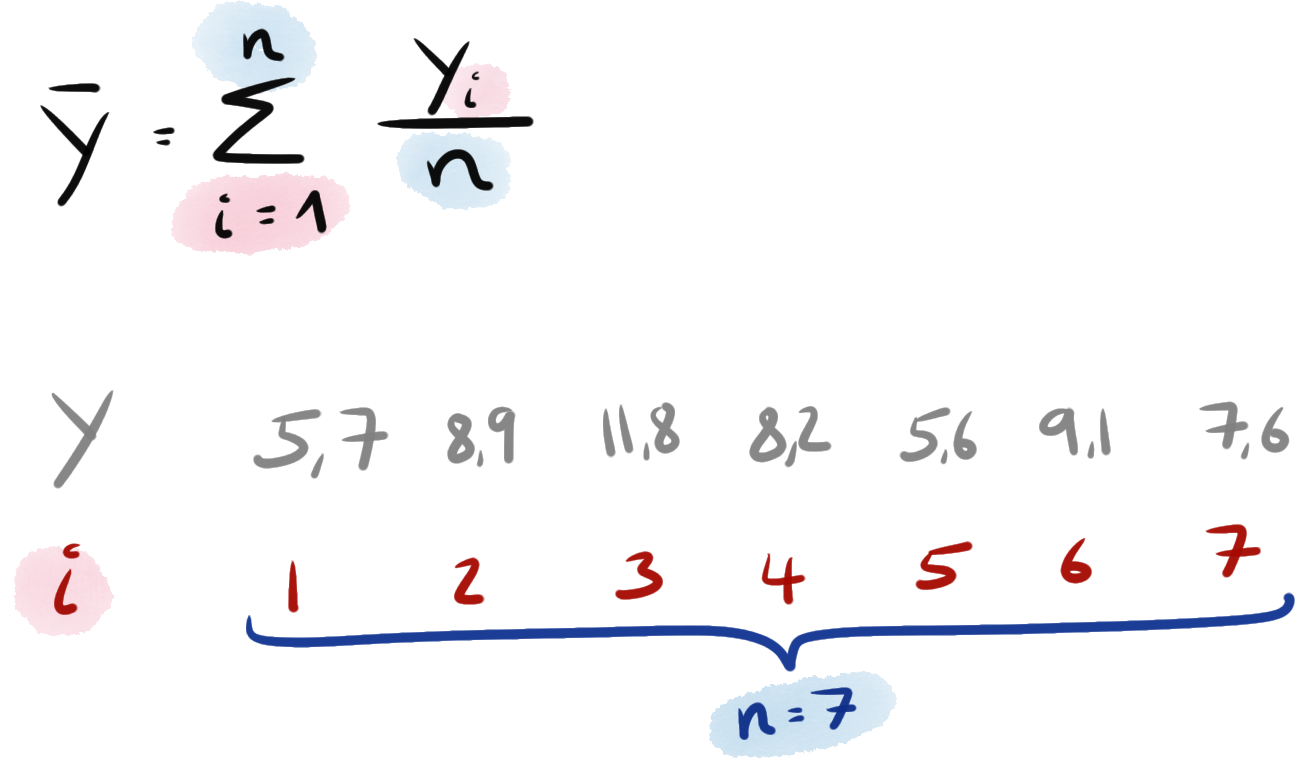
\includegraphics[width=1\textwidth,height=\textheight]{./images/index-drawn.png}

}

\caption{\label{fig-index-drawn}Zusamenhang zwischen \(y\) sowie dem
Index \(i\) in der Formel für den Mittelwert.}

\end{figure}

In R können wir den Mittelwert einfach mit der Funktion \texttt{mean()}
berechnen. Wir wollen dann den Mittelwert noch auf die zweite
Kommastelle runden. Das machen wir dann mit der Funktion
\texttt{round()}.

\begin{Shaded}
\begin{Highlighting}[]
\NormalTok{y }\SpecialCharTok{\%\textgreater{}\%}\NormalTok{ mean }\SpecialCharTok{\%\textgreater{}\%} \FunctionTok{round}\NormalTok{(}\DecValTok{2}\NormalTok{)}
\end{Highlighting}
\end{Shaded}

\begin{verbatim}
[1] 8.13
\end{verbatim}

Wir erhalten das gleiche Ergebnis wie oben in unserer händischen
Rechnung. Die Hundeflöhe springen im Mittel 8.13 cm weit.

Der Mittelwert ist eine bedeutende Maßzahl der Normalverteilung. Daher
merken wir uns hier schon mal, dass wir den Mittelwert brauchen werden.
Auch wenn wir darüber nachdenken ob sich zwei Gruppen unterscheiden, so
nutzen wir hierzu den Mitelwert. Unterscheiden sich die \emph{mittleren}
Sprungweiten in {[}cm{]} von Hunde- und Katzenflöhen?

\hypertarget{spannweite}{%
\section{Spannweite}\label{spannweite}}

Die \emph{Spannweite} erlaubt uns zu überprüfen was die kleinste Zahl
und die größte Zahl ist. Also uns das Minimum und das Maximum einer
Zahlenreihe anzuschauen. Auf den ersten Blick mag das nicht so sinnig
sein, aber wenn wir uns hunderte von Beobachtungen anschauen, wollen wir
wissen, ob wir nicht einen Fehler bei Eintragen der Daten gemacht haben.
Wir wissen eigentlich, dass z.B keine negativen Zuwachsraten auftreten
können.

{\marginnote{\begin{footnotesize}Die Spannweite dient dazu in einem
Datensatz zu übersprüfen ob die \textbf{Spalte}, oder auch
\textbf{Variable} genannt, den richtigen Zahlenraum aufweist. Das machen
wir durch die Funktion \texttt{range()}.\end{footnotesize}}}

\[
y_{range} = y_{max} - y_{min} = 12.1 - 4.9 = 7.2
\] Die Hundeflöhe springen in einer Spannweite von 7.2 cm. Das kommt
einem \emph{normal} vor. Die Spannweite ist nicht übertrieben groß. Der
minimale Wert ist 4.9 und der maximale Wert it 12.1 und somit sind beide
Zahlen in Ordnung. Keine der beiden Zahlen ist übertrieben groß oder gar
negativ.

In R können wir die Spannweite mit \texttt{range()} wie folgt berechnen.
Wir erhalten den minmialen udn maximalen Wert.

\begin{Shaded}
\begin{Highlighting}[]
\FunctionTok{range}\NormalTok{(y) }
\end{Highlighting}
\end{Shaded}

\begin{verbatim}
[1]  5.6 11.8
\end{verbatim}

Wir merken uns, dass die Spannweite eine Maßzahl für die Validität der
Daten ist. Hat das Experiment geklappt oder kamen da nur komische Zahlen
bei raus, die wir so in der Realität nicht erwarten würden. Zum Beispiel
negative Sprungweiten, weil wir einmalauf das Minuszeichen gekommen
sind.

\hypertarget{varianz}{%
\section{Varianz}\label{varianz}}

Bis jetzt können wirmit dem Mittelwert \(\bar{y}\) die Lage oder den
Mittelpunkt unserer Zahlenreihe beschreiben. Uns fehlt damit aber die
Information über die Streuung der Zahlen. Sind die Zahlen alle eher
gleich oder sehr verschieden? Liegen die Zahlen daher alle bei dem
Mittelwert oder sind die Zahlen weit um den Mittelwert gestreut.

Die Streuung der Zahlen um den Mittelwert beschreibt die Varianz oder
auch \(s^2\). Wir berechnen die Varianz indem wir von jeder Zahl den
Mittelwert aller Zahlen abziehen und dann das Ergebnis quadrieren. Das
machen wir für alle Zahlen und addieren dann die Summe auf. Wir erhalten
die \emph{Quadratsumme} von \(y\).

{\marginnote{\begin{footnotesize}\textbf{Abweichungsquadrate} sind ein
wichtiges Konzept in der Statistik. Wenn wir wissen wollen, wie groß
eine Abweichung von einer Zahl zu einer anderen ist, dann nutzen wir
immer das Quadrat der Abweichung und bilden die
Quadratsumme..\end{footnotesize}}}

\[
s^2 = \sum_{i=1}^n\cfrac{(y_i - \bar{y})^2}{n-1} = \cfrac{(5.7 -
8.13)^2 + ... + (7.6 - 8.13)^2}{7-1} = 4.6
\]

Die Varianz berschreibt also die Streuung der Zahlen \emph{im Quadrat}
um den Mittelwert. Das heißt in unserem Beispiel, dass die Sprungweite
eine Varianz von 4.6 cm\(^2\) hat. Wir können Quadratzentimeter schlecht
interpretieren. Deshalb führen wir gleich die Wuzel der Varianz ein: die
Standardabweichung.

In R lässt sich die Varianz einfach durch die Funktion \texttt{var()}
berechnen.

\begin{Shaded}
\begin{Highlighting}[]
\NormalTok{y }\SpecialCharTok{\%\textgreater{}\%}\NormalTok{ var }\SpecialCharTok{\%\textgreater{}\%} \FunctionTok{round}\NormalTok{(}\DecValTok{2}\NormalTok{) }
\end{Highlighting}
\end{Shaded}

\begin{verbatim}
[1] 4.6
\end{verbatim}

Wir benötigen die Varianz häufig nur als Zwischenschritt um die
Standardabweichung zu berechnen. Das Konzept der Abweichungsquadrate
benötigen wir aber in der Varianzanalyse (ANOVA) und für die
Beschreibung einer Normalverteilung.

\hypertarget{standardabweichung}{%
\section{Standardabweichung}\label{standardabweichung}}

Die \emph{Standardabweichugn} ist die Wurzel der Varianz. Wo die Varianz
die Abweichung der Sprungweite in {[}cm\(^2\){]} beschreibt, beschreibt
die Standardabweichung die Streung der Sprungweite in {[}cm{]}.

\[
s = \sqrt{s^2} = \sqrt{4.6} = 2.14
\] {\marginnote{\begin{footnotesize}Wir schreiben immer den Mittelwert
plusminus die Standardabweichung. Also immer
\(\bar{y} \pm s\).\end{footnotesize}}}

Wir können also schreiben, dass die Flöhe im Mittel 8.13 \(\pm\) 2.14cm
weit springen. Somit haben wir die Lage und die Streuung der Zahlenreihe
\(y\) der Sprungweite in {[}cm{]} mit zwei Zahlen beschrieben.

In R können wir die Standardabweichung einfach mit der Funktion
\texttt{sd()} berechnen.

\begin{Shaded}
\begin{Highlighting}[]
\NormalTok{y }\SpecialCharTok{\%\textgreater{}\%}\NormalTok{ sd }\SpecialCharTok{\%\textgreater{}\%} \FunctionTok{round}\NormalTok{(}\DecValTok{2}\NormalTok{) }
\end{Highlighting}
\end{Shaded}

\begin{verbatim}
[1] 2.14
\end{verbatim}

\hypertarget{mittelwert-und-varianz---eine-herleitung}{%
\section{Mittelwert und Varianz - eine
Herleitung}\label{mittelwert-und-varianz---eine-herleitung}}

Was ist der Mitelwert und die Varianz genau? Schauen wir uns das einmal
in Abbildung~\ref{fig-mean-drawn} an. Die graue Linie oder Grade
beschreibt den Mittelwert der fünf Beobachtungen. Die fünf Beobachtungen
sind als blaue Punkt dargestellt. Auf der x-Achse ist nur der Index des
Punktes. Das heißt \(y_1\) ist der erste Punkte, das der Index \(i\)
gleich 1 ist.

\begin{figure}

{\centering 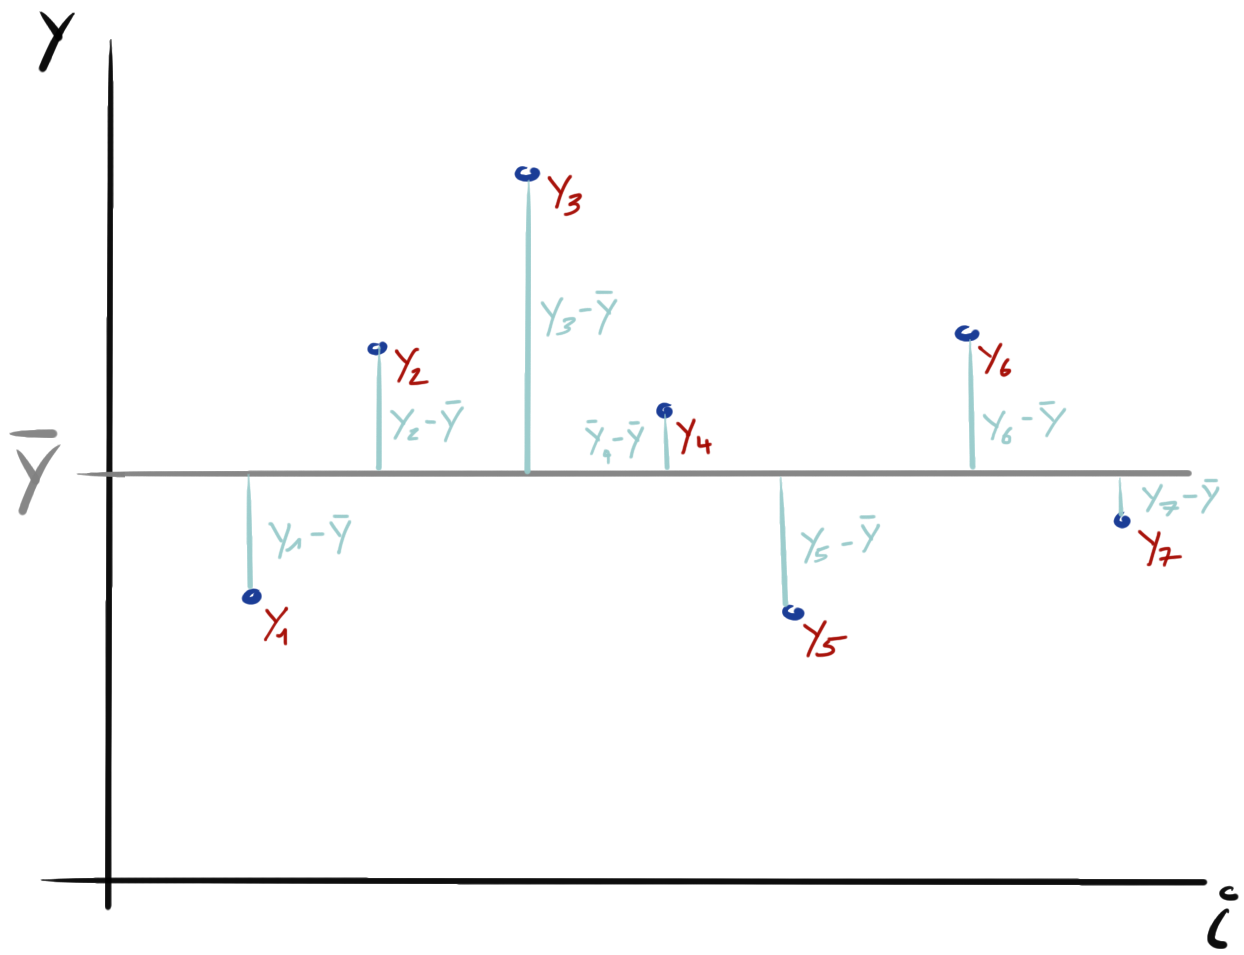
\includegraphics[width=1\textwidth,height=\textheight]{./images/mean-drawn.png}

}

\caption{\label{fig-mean-drawn}Die graue Linie beschreibt den Mittelwert
der genau so durch die blauen Punkte geht, dass die Abstände der Punkte
oberhalb und unterhalb zu Null aufaddieren. Die Linie liegt in der Mitte
der Punkte. Die quadrierten Abstände sind die Varainz der blauen Punkte.
Auf der x-Achse ist der Index des Punktes eingetragen.}

\end{figure}

Wenn wir die Summe der Abweichungen von \(y_1\) bis \(y_5\) zu dem
Mittelwert bilden, so wird diese Summe 0 sein. Der Mittelwert liegt
genau in der Mitte der Punkte. In unserem Beispiel ist der Mittelwert
\(\bar{y} = 5.8\). Wi können jetzt die Abstände wie in der folgenden
Tabelle berechnen.

\begin{figure*}

\begin{longtable}[]{@{}
  >{\centering\arraybackslash}p{(\columnwidth - 8\tabcolsep) * \real{0.1170}}
  >{\centering\arraybackslash}p{(\columnwidth - 8\tabcolsep) * \real{0.0638}}
  >{\centering\arraybackslash}p{(\columnwidth - 8\tabcolsep) * \real{0.3191}}
  >{\centering\arraybackslash}p{(\columnwidth - 8\tabcolsep) * \real{0.2340}}
  >{\centering\arraybackslash}p{(\columnwidth - 8\tabcolsep) * \real{0.2660}}@{}}
\toprule()
\begin{minipage}[b]{\linewidth}\centering
Index \(i\)
\end{minipage} & \begin{minipage}[b]{\linewidth}\centering
y
\end{minipage} & \begin{minipage}[b]{\linewidth}\centering
\(\boldsymbol{y_i - \bar{y}}\)
\end{minipage} & \begin{minipage}[b]{\linewidth}\centering
Wert
\end{minipage} & \begin{minipage}[b]{\linewidth}\centering
\(\boldsymbol{\epsilon}\)
\end{minipage} \\
\midrule()
\endhead
1 & 5.7 & \(y_1 - \bar{y}\) & \(5.7 - 8.13 = -2.43\) & \(\epsilon_1\) \\
2 & 8.9 & \(y_2 - \bar{y}\) & \(8.9 - 8.13 = 0.77\) & \(\epsilon_2\) \\
3 & 11.8 & \(y_3 - \bar{y}\) & \(11.8 - 8.13 = 3.67\) &
\(\epsilon_3\) \\
4 & 8.2 & \(y_4 - \bar{y}\) & \(8.2 - 8.13 = 0.07\) & \(\epsilon_4\) \\
5 & 5.6 & \(y_5 - \bar{y}\) & \(5.6 - 8.13 = -2.53\) & \(\epsilon_5\) \\
6 & 9.1 & \(y_4 - \bar{y}\) & \(9.1 - 8.13 = 0.97\) & \(\epsilon_4\) \\
7 & 7.6 & \(y_5 - \bar{y}\) & \(7.6 - 8.13 = -0.53\) & \(\epsilon_5\) \\
\bottomrule()
\end{longtable}

\end{figure*}

Wir nennen die Abstände \(y_i - \bar{y}\) nach dem griechischen
Buchstaben Epsilon \(\epsilon\). Das \(\epsilon\) soll an das \(e\) von
\emph{Error} erinnern. So meint dann \emph{Error} eben auch Abweichung.
Ja, es gibt hier viele Worte für das gleiche Konzept.

Wir berechnen einen Mittelwert von den Epsilons mit
\(\bar{\epsilon} = 0\). Ein Mittelwert nahe Null bzw. von Null wundert
uns nicht. Wir haben die Gerade ja so gebaut, das nach oben und unten
die gleichen Abstände sind. Die Varianz \(s^2\) der \(y\) ist
\(s_y^2 = 4.599\) und die Varianz von \(\epsilon\) ist
\(s_{\epsilon}^2 = 4.599\). In beiden Fällen ist die Zahl gleich.

\hypertarget{standardfehler-oder-standard-error-se}{%
\section{Standardfehler oder Standard Error
(SE)}\label{standardfehler-oder-standard-error-se}}

Wenn wir den Mittelwert der Sprungweiten berichten dann gehört die
Standardabweichung der Sprungweiten mit als beschreibendes Maß dazu. Wir
berichten keinen Mittelwert ohne Standardabweichung.

Nun ist es aber so, dass der Mittelwert und die Standardabweichung von
der Fallzahl abhängen. Je mehr Fallzahl bzw. Beoabchtungen wir haben,
desto genauer wird der Mittelwert sein. Oder anders ausgedrückt
\(\bar{y}\) wird sich \(\mu_y\) annähern. Das gleiche gilt auch für die
Standardabweichung \(s_y\), die sich \(\sigma_y\) mit steigender
Fallzahl annähert.

Aus diesem Grund brauchen wir noch einen Fehler bzw. eine Maßzahl für
die Streuung, die unabhängig von der Fallzahl ist. Wir skalieren also
die Standardabweichung mit der Fallzahl indem wir die Standardbweichung
durch die Wurzel der Fallzahl teilen.

\[
SE = \cfrac{s}{\sqrt{n}} = \cfrac{2.14}{2.65} = 0.81
\]

Wir müssten ein Paket in R laden um den Standardfehler zu berechnen. Das
Laden von zusätzlichen Paketen wollen wir hier aber vermeiden; wir
können den Standardfehler auch einfach selber berechnen.

\begin{Shaded}
\begin{Highlighting}[]
\NormalTok{se }\OtherTok{\textless{}{-}} \FunctionTok{sd}\NormalTok{(y)}\SpecialCharTok{/}\FunctionTok{sqrt}\NormalTok{(}\FunctionTok{length}\NormalTok{(y))}
\NormalTok{se }\SpecialCharTok{\%\textgreater{}\%} \FunctionTok{round}\NormalTok{(}\DecValTok{2}\NormalTok{)}
\end{Highlighting}
\end{Shaded}

\begin{verbatim}
[1] 0.81
\end{verbatim}

Wir erhalten einen Standardfehler von 0.81. Diese Zahl ist in dem Sinne
nicht zu interpretieren, da wir hier nur Experimente losgelöst von deren
Fallzahl miteinander vergleichen können. Auf der anderen Seite können
wir ohne die berichtete Fallzahl nicht vom Standardfehler auf die
Standardabweichung schließen.

{\marginnote{\begin{footnotesize}Wir berichten den
\textbf{Standardfehler} immer zusammen mit der Fallzahl, so dass die
Standardabweichung berechnet werden kann.\end{footnotesize}}}

Wir benötigen den Standardfehler eigentlich nicht zum Berichten von
Ergebnissen. Der Standardfehler ist nicht als Zahl interpretierbar und
somit eine reine statistische Größe. Tabelle~\ref{tbl-comp-stand-sem}
zeigt die Zusammenfassung und den Vergleich von Standardabweichung und
Standardfehler.

\hypertarget{tbl-comp-stand-sem}{}
\begin{longtable}[]{@{}
  >{\raggedright\arraybackslash}p{(\columnwidth - 2\tabcolsep) * \real{0.5000}}
  >{\raggedright\arraybackslash}p{(\columnwidth - 2\tabcolsep) * \real{0.5000}}@{}}
\caption{\label{tbl-comp-stand-sem}Zusammenfassung und Vergleich von
Standardabweichung und Standardfehler}\tabularnewline
\toprule()
\begin{minipage}[b]{\linewidth}\raggedright
Standardabweichung
\end{minipage} & \begin{minipage}[b]{\linewidth}\raggedright
Standardfehler
\end{minipage} \\
\midrule()
\endfirsthead
\toprule()
\begin{minipage}[b]{\linewidth}\raggedright
Standardabweichung
\end{minipage} & \begin{minipage}[b]{\linewidth}\raggedright
Standardfehler
\end{minipage} \\
\midrule()
\endhead
\ldots{} ist eine Aussage über die Streuung der erhobenen Werte einer
Stichprobe. & \ldots{} ist eine Aussage über die Genauigkeit des
Mittelwertes einer Stichprobe. \\
\ldots{} hängt von der biologischen Variabilität ab. & \ldots{} abhängig
von der Messgenauigkeit \\
\ldots{} ist ein beschreibendes Maß. & \ldots{} ist ein statistisches
Maß. \\
\ldots{} ist nur wenig durch die Größe der Stichprobe beineinflussbar. &
\ldots{} steht im direkten Verhältnis zur Größe der Stichprobe. \\
\bottomrule()
\end{longtable}

\marginnote{\begin{footnotesize}

Der Standardfehler oder Standard Error (SE) oder Standard Error of the
Mean (SEM) wird uns wieder beim statistischen Testen und dem t-Test
begegnen.

\[
T_{calc} = \cfrac{\bar{y_1} - \bar{y_2}}{s_p \cdot \sqrt{\tfrac{2}{n}}} \approx \cfrac{\bar{y_1} - \bar{y_2}}{SEM}
\]

Der Nenner beim t-Test kann als Standardfehler gesehen werden. Wir
benötigen den Standardfehler also im Kontext des statistischen Testen
als eine statististische Maßzahl.

\end{footnotesize}}

\begin{tcolorbox}[enhanced jigsaw, coltitle=black, titlerule=0mm, bottomrule=.15mm, opacityback=0, opacitybacktitle=0.6, leftrule=.75mm, title=\textcolor{quarto-callout-note-color}{\faInfo}\hspace{0.5em}{Standardfehler wird in der Metaanalyse genutzt}, toprule=.15mm, bottomtitle=1mm, toptitle=1mm, left=2mm, breakable, arc=.35mm, colback=white, rightrule=.15mm, colbacktitle=quarto-callout-note-color!10!white, colframe=quarto-callout-note-color-frame]
Der Standardfehler ist bedeutend in der Metaanalyse. Also dem
gemeinsamen Auswerten von mehreren \emph{klinischen} Studien. Du kannst
im Buch
\href{https://bookdown.org/MathiasHarrer/Doing_Meta_Analysis_in_R/effects.html}{Doing
Meta-Analysis with R: A Hands-On Guide} mehr darüber erfahren. Wir
nutzen keine Metaanalysen in den Grundlagenveranstaltungen.
\end{tcolorbox}

\hypertarget{median}{%
\section{Median}\label{median}}

Wir wollen uns jetzt noch eine andere Art der Zusammenfassung von Zahlen
anschauen. Anstatt \emph{mit den Zahlen} zu rechnen, sortieren wir jetzt
die Zahlen aus dem Vektor \(y = \{5.7, 8.9, 11.8, 8.2, 5.6, 9.1, 7.6\}\)
nach dem Rang. Wir rechnen dann \emph{mit den Rängen}. Die kleinste Zahl
kriegt den kleinsten Rang. Wir können R nutzen über due Funktion
\texttt{sort()} um den Vektor \(y\) zu sortieren.

\begin{Shaded}
\begin{Highlighting}[]
\NormalTok{y }\SpecialCharTok{\%\textgreater{}\%} \FunctionTok{sort}\NormalTok{()}
\end{Highlighting}
\end{Shaded}

\begin{verbatim}
[1]  5.6  5.7  7.6  8.2  8.9  9.1 11.8
\end{verbatim}

Der Median \(\tilde{y}\) ist die mittlere Zahl eines Zahlenvektors. Wir
haben hier sieben Zahlen, also ist der Median die vierte Zahl. Wir
müssen hier aber zwischen einr ungeraden Anzahl und einer geraden Anzahl
unterscheiden.

\begin{itemize}
\tightlist
\item
  \textbf{Ungerade Anzahl} von Zahlen, der Median ist die mittlere Zahl
  des Vektors \(y\): \[
  5.6,  5.7,  7.6,  \underbrace{8.2,}_{Median}  8.9,  9.1, 11.8
  \]
\end{itemize}

In R können wir den Median einfach mit der Funktion
\texttt{median()}berechnen.

\begin{Shaded}
\begin{Highlighting}[]
\FunctionTok{median}\NormalTok{(y) }
\end{Highlighting}
\end{Shaded}

\begin{verbatim}
[1] 8.2
\end{verbatim}

\begin{itemize}
\tightlist
\item
  \textbf{Gerade Anzahl} von Zahlen, der Median ist der Mittelwert der
  \emph{beiden} mittleren Zahlen des Vektors \(y\): \[
  5.6,  5.7,  7.6,  \underbrace{8.2, 8.9,}_{Median = \tfrac{8.2+8.9}{2}=8.55} 9.1, 11.8, \color{blue}{13.1}
  \]
\end{itemize}

In R können wir den Median wieder einfach mit der Funktion
\texttt{median()}berechnen. Wir müssen nur die Zahl 13.1 zu dem Vektor
\texttt{y} mit der Funktion \texttt{c()} hinzufügen.

\begin{Shaded}
\begin{Highlighting}[]
\FunctionTok{c}\NormalTok{(y, }\FloatTok{13.1}\NormalTok{) }\SpecialCharTok{\%\textgreater{}\%} \FunctionTok{median}\NormalTok{() }
\end{Highlighting}
\end{Shaded}

\begin{verbatim}
[1] 8.55
\end{verbatim}

{\marginnote{\begin{footnotesize}Wenn der \textbf{Mittelwert} stark von
dem \textbf{Median} abweicht, deutet dies auf eine schiefe Verteilung
oder aber Ausreißer in den Daten hin. Wir müssen dann in der
explorativen Datenanalyse der Sachlage nachgehen\end{footnotesize}}}

Der Median ist eine Alternative zu dem Mitelwert. Insbesondere in
Fällen, wo es sehr große Zahlen gibt, die den Mittelwert in der Aussage
\emph{verzerren}, kann der Median sinnvoll sein.

\begin{tcolorbox}[enhanced jigsaw, coltitle=black, titlerule=0mm, bottomrule=.15mm, opacityback=0, opacitybacktitle=0.6, leftrule=.75mm, title=\textcolor{quarto-callout-tip-color}{\faLightbulb}\hspace{0.5em}{Median versus Mittelwert}, toprule=.15mm, bottomtitle=1mm, toptitle=1mm, left=2mm, breakable, arc=.35mm, colback=white, rightrule=.15mm, colbacktitle=quarto-callout-tip-color!10!white, colframe=quarto-callout-tip-color-frame]
Zur Veranschaulichung des Unterschiedes zwischen Median und Mittelwert
nehmen wir die Mietpreise in New York. Der \emph{mittlere} Mietpreis für
eine 2-Zimmerwohnung in Manhattan liegt bei 5000\$ pro Monat. In den
\emph{mittleren} Mietpreis gehen aber auch die Mieten der Billionaires'
Row mit ein. Der \emph{mediane} Mietpreis liegt bei 4000\$. Die hohen
Mieten \emph{ziehen} den Mittelwert nach rechts.
\end{tcolorbox}

\hypertarget{quantile-und-quartile}{%
\section{Quantile und Quartile}\label{quantile-und-quartile}}

Bei dem Mittelwert beschreibt die Standardabweichung die Streuung der
Daten um den Mitelwert. Bei dem Median sind dies die \emph{Quartile}.
Die Quartile beschreiben die Streuung der Daten um den Median. Um die
Quartile bestimmen zu können, teilen wir die Daten in 100 Quantile. Du
kannst dir Quantile wie Prozente vorstellen. Wir schneiden die Daten
also in 100 Scheiben. Das geht natürlich erst wirklich, wenn wir hundert
Zahlen haben. Deshalb hilft man sich mit Qua\textbf{r}tilen - von
Quarta, ein Viertel - aus. Tabelle~\ref{tbl-quart-quant} zeigt den
Zusammenhang.

\hypertarget{tbl-quart-quant}{}
\begin{longtable}[]{@{}ccc@{}}
\caption{\label{tbl-quart-quant}Zusammenfassung und Vergleich von
Quantilen, Quartilen und Median}\tabularnewline
\toprule()
Quantile & Quartile & Median \\
\midrule()
\endfirsthead
\toprule()
Quantile & Quartile & Median \\
\midrule()
\endhead
25\% Quantile & 1\(^{st}\) Quartile & \\
50\% Quantile & 2\(^{nd}\) Quartile & Median \\
75\% Quantile & 3\(^{rd}\) Quartile & \\
\bottomrule()
\end{longtable}

Wir bestimmen die Quartile wie den Median. Wir müssen unterscheiden, ob
wir eine ungerade Anzahl an Zahlen oder eine gerade Anzahl an Zahlen
vorliegen haben.

\begin{itemize}
\item
  \textbf{Ungerade Anzahl} von Zahlen, das 1\(^{st}\) Quartile ist die
  mittlere Zahl des unteren Mittels und das 3\(^{rd}\) Quartile ist die
  mittlere Zahl des oberen Mittels des Vektors \(y\): \[
  5.6,  \underbrace{5.7,}_{1st\ Quartile}  7.6,  8.2,  8.9,  \underbrace{9.1,}_{3rd\ Quartile} 11.8
  \]
\item
  \textbf{Gerade Anzahl} von Zahlen, das 1\(^{st}\) Quartile ist der
  Mittelwert der beiden mittleren Zahl des unteren Mittels und das
  3\(^{rd}\) Quartile ist der Mitelwert der beiden mittleren Zahlen des
  oberen Mittels des Vektors \(y\): \[
  5.6,  \underbrace{5.7, 7.6,}_{1st\ Quartile = \tfrac{5.7+7.6}{2}=6.65}    8.2,  8.9,  \underbrace{9.1, 11.8}_{3rd\ Quartile = \tfrac{9.1+11.8}{2}=10.45} \color{blue}{13.1}
  \]
\end{itemize}

{\marginnote{\begin{footnotesize}Das \textbf{95\% Quantile} und das
\textbf{97.25\% Quantile} werden wir später nochmal im statistischen
Testen brauchen. Auch hier ist die Idee, dass wir die Daten in hundert
Teile schneiden und uns dann die extremen Zahlen
anschauen.\end{footnotesize}}}

In R können wir den Median einfach mit der Funktion \texttt{quantile()}
berechnen. Wir berechnen hier das 25\% Quantile also das 1\(^{st}\)
Quartile sowie das 50\% Quantile also den Median und das 75\% Quantile
also das 3\(^{rd}\) Quartile.

\begin{Shaded}
\begin{Highlighting}[]
\NormalTok{y }\SpecialCharTok{\%\textgreater{}\%} \FunctionTok{quantile}\NormalTok{(}\AttributeTok{probs =} \FunctionTok{c}\NormalTok{(}\FloatTok{0.25}\NormalTok{, }\FloatTok{0.5}\NormalTok{, }\FloatTok{0.75}\NormalTok{)) }\SpecialCharTok{\%\textgreater{}\%} \FunctionTok{round}\NormalTok{(}\DecValTok{2}\NormalTok{)}
\end{Highlighting}
\end{Shaded}

\begin{verbatim}
 25%  50%  75% 
6.65 8.20 9.00 
\end{verbatim}

\begin{Shaded}
\begin{Highlighting}[]
\FunctionTok{c}\NormalTok{(y, }\FloatTok{13.1}\NormalTok{) }\SpecialCharTok{\%\textgreater{}\%} \FunctionTok{quantile}\NormalTok{(}\AttributeTok{probs =} \FunctionTok{c}\NormalTok{(}\FloatTok{0.25}\NormalTok{, }\FloatTok{0.5}\NormalTok{, }\FloatTok{0.75}\NormalTok{)) }\SpecialCharTok{\%\textgreater{}\%} \FunctionTok{round}\NormalTok{(}\DecValTok{2}\NormalTok{) }
\end{Highlighting}
\end{Shaded}

\begin{verbatim}
 25%  50%  75% 
7.12 8.55 9.77 
\end{verbatim}

Warum unterscheiden sich die händisch berechneten Quartile von den
Quartilen aus R? Es gibt verschiedene Arten der Berechnung. In der
Klausur nutzen wir die Art und Weise wie die händische Berechnung hier
beschrieben ist. Später in der Anwendung nehmen wir die Werte, die R
ausgibt. Die Abweichungen sind so maginal, dass wir diese Abweichungen
in der praktischen Anwendung ignorieren wollen.

\hypertarget{interquartilesabstand-iqr}{%
\section{Interquartilesabstand (IQR)}\label{interquartilesabstand-iqr}}

Der Interquartilesabstand (IQR) beschreibt den Abstand zwischen dem
1\(^{st}\) Quartile und dem 3\(^{rd}\) Quartile. Daher ist der
Interquartilesabstand (IQR) ähnlich der Spannweite zwischen dem
maximalen und minimalen Wert. Wir benötigen das Interquartilesabstand
(IQR) in der explorativen Datenanalyse wenn wir einen Boxplot erstellen
wollen.

\[
IQR = 3^{rd}\,\mbox{Quartile} - 1^{st}\,\mbox{Quartile} = 9.1 - 5.7 = 3.4
\]

\hypertarget{sec-desc-group-by}{%
\section{Zusammenfassen von Daten per Faktor}\label{sec-desc-group-by}}

Gut und soll ich jetzt für jeden Faktorlevel überall den Mittelwert mit
\texttt{mean()} berechnen? Geht das nicht einfacher? Ja, geht es. Im
folgenden siehst du, wie du den verschiedene deskriptive Maßzahlen in
einem Rutsch berechnen kannst.

\begin{Shaded}
\begin{Highlighting}[]
\NormalTok{data\_tbl }\SpecialCharTok{\%\textgreater{}\%}
  \FunctionTok{mutate}\NormalTok{(}\AttributeTok{animal =} \FunctionTok{as\_factor}\NormalTok{(animal)) }\SpecialCharTok{\%\textgreater{}\%}
  \FunctionTok{group\_by}\NormalTok{(animal) }\SpecialCharTok{\%\textgreater{}\%}
  \FunctionTok{summarise}\NormalTok{(}\AttributeTok{mean =} \FunctionTok{mean}\NormalTok{(jump\_length),}
            \AttributeTok{sd =} \FunctionTok{sd}\NormalTok{(jump\_length),}
            \AttributeTok{median =} \FunctionTok{median}\NormalTok{(jump\_length),}
            \AttributeTok{quantiles =} \FunctionTok{quantile}\NormalTok{(jump\_length, }
                                 \AttributeTok{probs =} \FunctionTok{c}\NormalTok{(}\FloatTok{0.25}\NormalTok{, }\FloatTok{0.5}\NormalTok{, }\FloatTok{0.75}\NormalTok{))) }\SpecialCharTok{\%\textgreater{}\%} 
  \FunctionTok{mutate}\NormalTok{(}\FunctionTok{across}\NormalTok{(}\FunctionTok{where}\NormalTok{(is.numeric), round, }\DecValTok{2}\NormalTok{))}
\end{Highlighting}
\end{Shaded}

\begin{verbatim}
# A tibble: 6 x 5
# Groups:   animal [2]
  animal  mean    sd median quantiles
  <fct>  <dbl> <dbl>  <dbl>     <dbl>
1 dog     8.13  2.14    8.2      6.65
2 dog     8.13  2.14    8.2      8.2 
3 dog     8.13  2.14    8.2      9   
4 cat     4.74  1.9     4.3      3.65
5 cat     4.74  1.9     4.3      4.3 
6 cat     4.74  1.9     4.3      5.75
\end{verbatim}

\hypertarget{sec-eda-ggplot}{%
\chapter{Visualisierung von Daten}\label{sec-eda-ggplot}}

\emph{Version vom September 14, 2022 um 08:47:09}

{\marginnote{\begin{footnotesize}Wir nennen eine Abbildung auch häufig
Plot. Das ist der englische Begriff und hat nichts in unserem Kontext
mit einer Fläche zu tun.\end{footnotesize}}}

Ein wichtiger Teil in der Analyse von Daten ist die Visualisierung. Wir
glauben keine Auswertung eines mathematischen Algorithmus, wenn wir
nicht die Bestätigung in einer Abbildung sehen. Daher ist die
Visualisierung die Grundlage für ein fundiertes, wissenschaftliches
Arbeiten. In diesem Kapitel stelle ich dir verschiedene Abbilungen vor,
die uns helfen werden zu Verstehen ob es einen Zusammenhang zwischen Y
und X gibt. Wir haben ein \(y\) vorliegen, was wir auf die y-Achse eines
Graphen legen und daneben dann mehrere Variablen bzw. Spalten die wir
\(x\) nennen. Eine der Variablen legen wir auf die x-Achse des Graphen.
Nach den anderen \(x\) färben wir die Abbildung ein.

\hypertarget{genutzte-r-pakete-fuxfcr-das-kapitel-2}{%
\section{Genutzte R Pakete für das
Kapitel}\label{genutzte-r-pakete-fuxfcr-das-kapitel-2}}

Wir wollen folgende R Pakete in diesem Kapitel nutzen.

\begin{Shaded}
\begin{Highlighting}[]
\NormalTok{pacman}\SpecialCharTok{::}\FunctionTok{p\_load}\NormalTok{(tidyverse, magrittr, readxl, ggmosaic, }
\NormalTok{               janitor, see, patchwork)}
\end{Highlighting}
\end{Shaded}

Am Ende des Kapitels findest du nochmal den gesamten R Code in einem
Rutsch zum selber durchführen oder aber kopieren.

\hypertarget{grundlagen-in-ggplot}{%
\section{Grundlagen in ggplot()}\label{grundlagen-in-ggplot}}

{\marginnote{\begin{footnotesize}Im Gegensatz zu dem Pipe-Operator
\texttt{\%\textgreater{}\%} nutzt ggplot den Operator \texttt{+} um die
verschiedenen ggplot Funktionen (\texttt{geom\_}) miteinander zu
verbinden.\end{footnotesize}}}

Wir nutzen in R das R Paket \texttt{ggplot2} um unsere Daten zu
visualisieren. Die zentrale Idee von \texttt{ggplot2} ist, dass wir uns
eine Abbildung wie ein Sandwich bauen. Zuerst legen wir eine Scheibe
Brot hin und legen uns dann Scheibe für Scheibe weitere Schichten
übereinander. Oder die Idee eines Bildes, wo wir erst die Leinwand
definieren und dann Farbschicht über Farbschicht auftragen. Das Konzept
von \texttt{ggplot2}ist schlecht zu be\emph{schreiben} deshalb habe ich
auch noch zwei Videos hierfür gemacht. Um den Prozess von
\texttt{ggplot2} zu visualisieren\ldots{}

\begin{tcolorbox}[enhanced jigsaw, coltitle=black, titlerule=0mm, bottomrule=.15mm, opacityback=0, opacitybacktitle=0.6, leftrule=.75mm, title=\textcolor{quarto-callout-tip-color}{\faLightbulb}\hspace{0.5em}{Grundlagen von ggplot() im Video}, toprule=.15mm, bottomtitle=1mm, toptitle=1mm, left=2mm, breakable, arc=.35mm, colback=white, rightrule=.15mm, colbacktitle=quarto-callout-tip-color!10!white, colframe=quarto-callout-tip-color-frame]
Du findest auf YouTube \href{https://youtu.be/SGwSVzJ9C-s}{Einführung in
R - Teil 16.0 - Trockenübung ggplot2 simpel und einfach erklärt} als
Video.

Sowie auch auf YouTube \href{https://youtu.be/SRRQQO3DXtc}{Einführung in
R - Teil 16.1 - Abbildungen mit ggplot in R erstellen. Idee und Konzept
von ggplot} als Video. Also alles nochmal als Video - vielleicht
einfacher nachzuvollziehen als in einem Fließtext.
\end{tcolorbox}

Die Funktion \texttt{ggplot()} ist die zentrale Funktion, die die
Leinwand erschafft auf der wir dann verschiedene Schichten aufbringen
werden. Diese Schichten heißen \texttt{geom}. Es gibt nicht nur ein
\texttt{geom} sondern mehrere. Zum Beispiel das \texttt{geom\_boxplot}
für die Erstellung von Boxplots, das \texttt{geom\_histogram} für die
Erstellung von Histogrammen.
\href{https://ggplot2.tidyverse.org/reference/index.html}{Die Auswahl
ist riesig}. Die einzelnen Schichten werden dann über den Operator
\texttt{+} miteinander verbunden. Soviel erstmal zur Trockenübung.
Schauen wir uns das ganze einmal an einem Beispiel an.

\hypertarget{datenbeispiel}{%
\subsection{Datenbeispiel}\label{datenbeispiel}}

Wir importieren den Datensatz \texttt{flea\_cat\_dog.xlsx} und wollen
einzelne Variablen visualisieren. Wir kennen den Datensatz schon aus dem
Kapitel~\ref{sec-example-2}. Dennoch nochmal hier der Datensatz in
Tabelle~\ref{tbl-cat-dog-ggplot}.

\begin{Shaded}
\begin{Highlighting}[]
\NormalTok{flea\_dog\_cat\_tbl }\OtherTok{\textless{}{-}} \FunctionTok{read\_excel}\NormalTok{(}\StringTok{"data/flea\_dog\_cat.xlsx"}\NormalTok{) }\SpecialCharTok{\%\textgreater{}\%} 
  \FunctionTok{mutate}\NormalTok{(}\AttributeTok{animal =} \FunctionTok{as\_factor}\NormalTok{(animal))}
\end{Highlighting}
\end{Shaded}

{\marginnote{\begin{footnotesize}Spaltennamen sind in \textbf{Englisch}
und haben \textbf{keine Leerzeichen}. Die Funktion
\texttt{clean\_names()} aus dem R Paket \texttt{janitor} ist hier eine
Hilfe.\end{footnotesize}}}

Im folgenden ist es wichtig, dass du dir die Spaltennamen merkst. Wir
können nur die exakten, wortwörtlichen Spaltennamen verwenden. Sonst
erhalten wir einen Fehler. Deshalb haben wir auch keine Leerzeichen in
den Spaltennamen.

\hypertarget{tbl-cat-dog-ggplot}{}
\begin{longtable}[]{@{}ccccc@{}}
\caption{\label{tbl-cat-dog-ggplot}Beispieldatensatz für Eigenschaften
von Flöhen von zwei Tierarten.}\tabularnewline
\toprule()
animal & jump\_length & flea\_count & grade & infected \\
\midrule()
\endfirsthead
\toprule()
animal & jump\_length & flea\_count & grade & infected \\
\midrule()
\endhead
dog & 5.7 & 18 & 8 & 0 \\
dog & 8.9 & 22 & 8 & 1 \\
dog & 11.8 & 17 & 6 & 1 \\
dog & 8.2 & 12 & 8 & 0 \\
dog & 5.6 & 23 & 7 & 1 \\
dog & 9.1 & 18 & 7 & 0 \\
dog & 7.6 & 21 & 9 & 0 \\
cat & 3.2 & 12 & 7 & 1 \\
cat & 2.2 & 13 & 5 & 0 \\
cat & 5.4 & 11 & 7 & 0 \\
cat & 4.1 & 12 & 6 & 0 \\
cat & 4.3 & 16 & 6 & 1 \\
cat & 7.9 & 9 & 6 & 0 \\
cat & 6.1 & 7 & 5 & 0 \\
\bottomrule()
\end{longtable}

\hypertarget{erste-abbildung-in-ggplot}{%
\subsection{Erste Abbildung in
ggplot()}\label{erste-abbildung-in-ggplot}}

Der folgende R Code erstellt die Leinwand in der
Abbildung~\ref{fig-ggplot-1} für die folgende, zusätzliches Schichten
(\texttt{geom}).

\begin{Shaded}
\begin{Highlighting}[]
\FunctionTok{ggplot}\NormalTok{(}\AttributeTok{data =}\NormalTok{ flea\_dog\_cat\_tbl, }
       \FunctionTok{aes}\NormalTok{(}\AttributeTok{x =}\NormalTok{ animal , }\AttributeTok{y =}\NormalTok{ jump\_length))}
\end{Highlighting}
\end{Shaded}

Wir schauen uns einmal den Code im Detail an.

\begin{itemize}
\tightlist
\item
  \texttt{ggplot} ruft die Funktion auf. Die Funktion ist dafür da den
  Plot zu zeichnen.
\item
  \texttt{data\ =\ flea\_dog\_cat\_tbl} bennent den Datensatz aus dem
  der Plot gebaut werden soll.
\item
  \texttt{aes()}ist die Abkürzung für \emph{aesthetics} und beschreibt,
  was auf die x-Achse soll, was auf die y-Achse soll sowie ob es noch
  andere Faktoren in den Daten gibt.

  \begin{itemize}
  \tightlist
  \item
    \texttt{x} braucht den Spaltennamen für die Variable auf der
    x-Achse.
  \item
    \texttt{y} braucht den Spaltennamen für die Variable auf der
    y-Achse.
  \end{itemize}
\end{itemize}

{\marginnote{\begin{footnotesize}\textbf{Faktoren} meint hier andere
Gruppenvariablen. Variablen sind ein anderes Wort für Spalten. Also
Variablen die wir mit \texttt{as\_factor}erschaffen
haben.\end{footnotesize}}}

\begin{figure}

{\centering 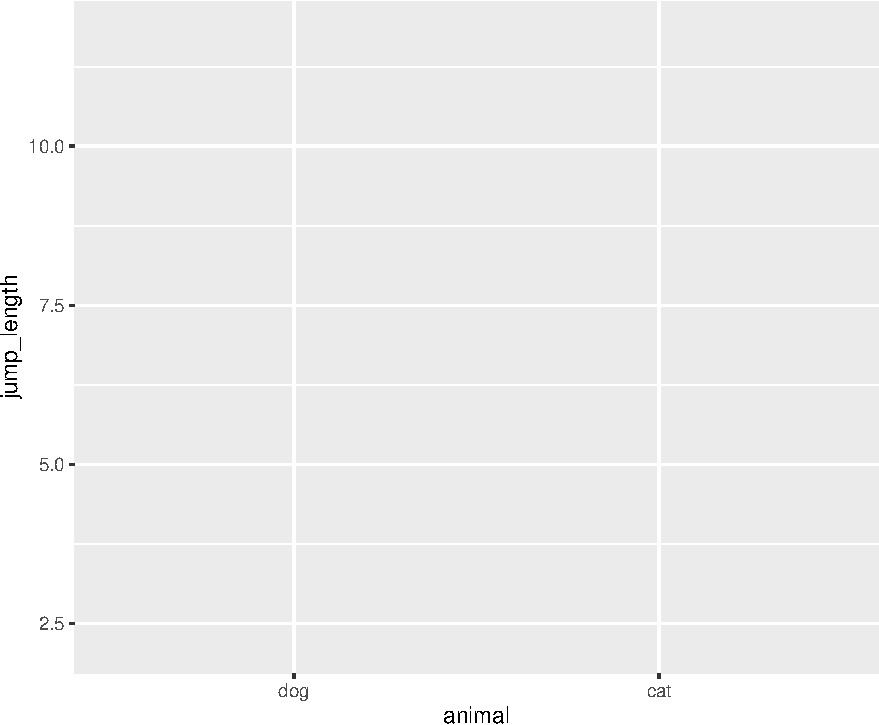
\includegraphics{./eda-ggplot_files/figure-pdf/fig-ggplot-1-1.pdf}

}

\caption{\label{fig-ggplot-1}Leere ggplot() Leinwand mit den Spalten
\texttt{animal} und \texttt{jump\_length} aus dem Datensatz
\texttt{flea\_dog\_cat\_tbl}.}

\end{figure}

Wir sehen, dass wir nichts sehen in Abbildung~\ref{fig-ggplot-1}. Der
Grund ist, dass wir noch kein \texttt{geom} hinzugefügt haben. Das
\texttt{geom} beschreibt nun wie die Zahlen in der Datentabelle
\texttt{flea\_dog\_cat\_tbl} visualisiert werden sollen.

\hypertarget{huxe4ufig-verwendete-abbildungen}{%
\section{Häufig verwendete
Abbildungen}\label{huxe4ufig-verwendete-abbildungen}}

In diesem Kapitel wollen wir durch die häufigsten und wichtigsten
Abbildungen in der explorativen Datenanalyse durchghen. Das wären im
folgenden diese Abbildungen:

\begin{itemize}
\tightlist
\item
  \textbf{Histogramm} in Kapitel~\ref{sec-eda-histogramm} für mehr als
  20 Beobachtungen (pro Gruppe). Wir nutzen ein Histogramm um die
  Verteilung einer Variable zu visualisieren.
\item
  \textbf{Boxplot} in Kapitel~\ref{sec-eda-boxplot} für 5 bis 20
  Beobachtungen (pro Gruppe). Ebenso wie bei einem Histogramm, geht es
  bei einem Boxplot auch um die Verteilung der einer Variable.
\item
  \textbf{Barplot} in Kapitel~\ref{sec-eda-barplot} für 5 und mehr
  Beobachtungen (pro Gruppe). Der Barplot oder das
  \textbf{Balkendiagramm} stellt den Mitelwert und die
  Standardabweichung da.
\item
  \textbf{Dotplot} in Kapitel~\ref{sec-eda-dotplot} für 3 bis 5
  Beobachtungen (pro Gruppe). Hier geht es weniger um die Verteilung der
  Variable, sondern darum die wenigen Beobachtungen zu visualisieren.
\item
  \textbf{Scatterplot} in Kapitel~\ref{sec-eda-scatter} für zwei
  kontinuierliche Variablen. Auch \textbf{xy-Plot} genannt. Die
  Abbildung, die dir bekannt sein müsste. Wir zeichnen hier eine Grade
  durch eine Punktewolke.
\item
  \textbf{Mosaicplot} in Kapitel~\ref{sec-eda-mosaic} für zwei diskrete
  Variablen. Eine etwas seltene Abbildung, wenn wir Variablen abbilden
  wollen, die diskret sind bzw. aus Kategorien bestehen.
\end{itemize}

{\marginnote{\begin{footnotesize}Konkret ist eine \textbf{Variable}
gleich einer \textbf{Spalte} in einem Datensatz.\end{footnotesize}}}

\begin{tcolorbox}[enhanced jigsaw, coltitle=black, titlerule=0mm, bottomrule=.15mm, opacityback=0, opacitybacktitle=0.6, leftrule=.75mm, title=\textcolor{quarto-callout-tip-color}{\faLightbulb}\hspace{0.5em}{Histogramm, Boxplot, Scatterplot und Mosaicplot im Video}, toprule=.15mm, bottomtitle=1mm, toptitle=1mm, left=2mm, breakable, arc=.35mm, colback=white, rightrule=.15mm, colbacktitle=quarto-callout-tip-color!10!white, colframe=quarto-callout-tip-color-frame]
Du findest auf YouTube \href{https://youtu.be/Zdw6NlLauNw}{Einführung in
R - Teil 16.2 - Histogramm, Boxplot, Scatterplot und Mosaicplot mit
ggplot in R} als Video. Weitere Videos werden dann noch folgen und
ergänzt.
\end{tcolorbox}

\hypertarget{sec-eda-histogramm}{%
\subsection{Histogramm}\label{sec-eda-histogramm}}

Wir nutzen für die Erstellung eines Histogramms den Datensatz
\texttt{dog\_fleas\_hist.csv}. Wir brauchen für ein anständiges
Histogramm, wo du auch was erkennen kannst, mindestens 20 Beobachtung.
Am besten mehr noch mhr Beobachtungen. Deshalb schauen wir uns jetzt
einmal 39 Hunde an und zählen wieviele Flöhe die Hunde jeweils haben,
dargestellt in der Spalte\texttt{flea\_count}. Darüber hinaus bestimmen
wir auch noch das mittlere Gewicht der Flöhe auf dem jeweiligen Hund,
dargestellt in der Spalte \texttt{flea\_weight}.

\begin{Shaded}
\begin{Highlighting}[]
\NormalTok{dog\_fleas\_hist\_tbl }\OtherTok{\textless{}{-}} \FunctionTok{read\_csv}\NormalTok{(}\StringTok{"data/dog\_fleas\_hist.csv"}\NormalTok{)}
\end{Highlighting}
\end{Shaded}

\hypertarget{tbl-cat-dog-histogram}{}
\begin{longtable}[]{@{}cc@{}}
\caption{\label{tbl-cat-dog-histogram}Beispieldatensatz für die Anzahl
an Flöhen auf 39 Hunden. Gezählt wurde die Anzahl an Flöhen
\texttt{flea\_count} und das gemittelte Gewicht der Flöhe
\texttt{flea\_weight}.}\tabularnewline
\toprule()
flea\_count & flea\_weight \\
\midrule()
\endfirsthead
\toprule()
flea\_count & flea\_weight \\
\midrule()
\endhead
0 & 0.00 \\
1 & 7.43 \\
4 & 21.04 \\
2 & 20.07 \\
1 & 21.90 \\
0 & 0.00 \\
2 & 24.96 \\
1 & 27.08 \\
5 & 16.58 \\
1 & 19.92 \\
0 & 0.00 \\
0 & 0.00 \\
2 & 24.63 \\
4 & 21.64 \\
3 & 20.97 \\
1 & 23.15 \\
0 & 0.00 \\
3 & 14.91 \\
1 & 19.39 \\
2 & 17.66 \\
1 & 19.15 \\
1 & 25.10 \\
2 & 26.38 \\
2 & 19.33 \\
2 & 13.29 \\
1 & 17.81 \\
0 & 0.00 \\
2 & 23.56 \\
1 & 18.64 \\
1 & 15.64 \\
3 & 19.88 \\
1 & 18.40 \\
1 & 25.17 \\
0 & 0.00 \\
0 & 0.00 \\
\bottomrule()
\end{longtable}

Tabelle~\ref{tbl-cat-dog-histogram} zeigt den Datensatz
\texttt{dog\_fleas\_hist.csv}. Wir wollen jetzt die Variable
\texttt{flea\_count} und \texttt{flea\_weight} jeweils abbilden. Wir
beginnen mit der diskreten Variable \texttt{flea\_count}. Im Gegensatz
zu der Variable \texttt{flea\_weight} haben wir bei der Anzahl gleiche
Zahlen vorliegen, die wir dann zusammen darstellen können.
Abbildung~\ref{fig-dotplot-flea-1} zeigt die Darstellung der Tabelle.
Auf der x-Achse ist die Anzahl an Flöhen dargestellt. Auf der y-Achse
die Anzahl der jeweiligen Anzahl an Flöhen. Das klingt jetzt etwas
schief, aber schauen wir uns die Abbilung näher an.

\begin{figure}

{\centering 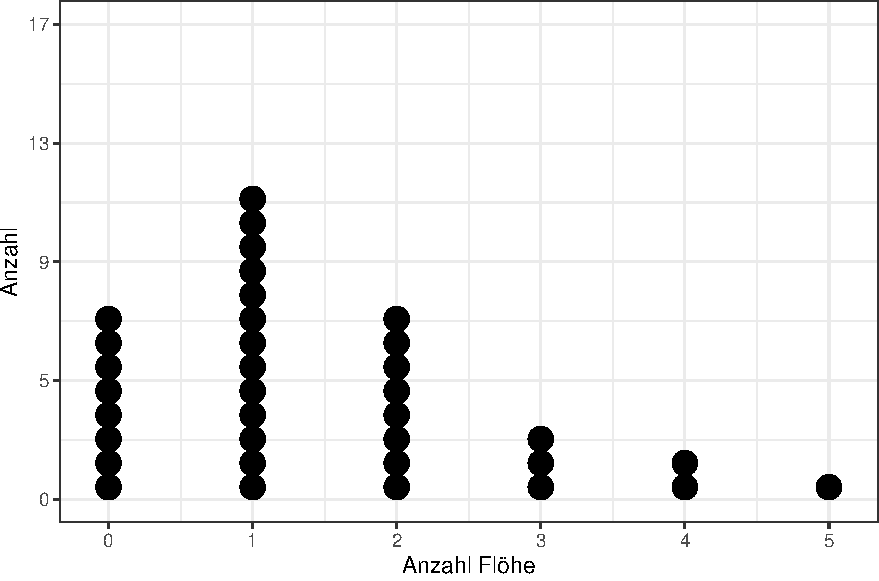
\includegraphics{./eda-ggplot_files/figure-pdf/fig-dotplot-flea-1-1.pdf}

}

\caption{\label{fig-dotplot-flea-1}Die Anzahl von Flöhen auf 39 Hunden.
Jeder Punkt entspricht einem Hund und der entsprechenden Anzahl an
Flöhen auf dem Hund.}

\end{figure}

Wir sehen in Abbildung~\ref{fig-dotplot-flea-1} das acht Hunde keine
Flöhe hatten - also eine Anzahl an Flöhen von 0. Auf der anderen Seite
hatten zwei Hunde vier Flöhe und ein Hund hatte sogar fünf Flöhe. Wir
sehen also die \emph{Verteilung} der Anzahl an Flöhen über alle unsere
39 Hundebeobachtungen.

Wir schauen uns aber die Verteilung der Anzahl an Flöhen meist nicht in
der Form von gestapelten Punkten an, sondern in der Form eines
Histogramms also einem Balkendiagramm.
Abbildung~\ref{fig-hist-flea-count} zeigt das Histogramm für die Anzahl
der Flöhe.

\begin{Shaded}
\begin{Highlighting}[]
\FunctionTok{ggplot}\NormalTok{(}\AttributeTok{data =}\NormalTok{ dog\_fleas\_hist\_tbl, }\FunctionTok{aes}\NormalTok{(}\AttributeTok{x =}\NormalTok{ flea\_count)) }\SpecialCharTok{+}
  \FunctionTok{geom\_histogram}\NormalTok{(}\AttributeTok{binwidth =} \DecValTok{1}\NormalTok{, }\AttributeTok{fill =} \StringTok{"gray"}\NormalTok{, }\AttributeTok{color =} \StringTok{"black"}\NormalTok{) }\SpecialCharTok{+}
  \FunctionTok{theme\_bw}\NormalTok{() }\SpecialCharTok{+}
  \FunctionTok{labs}\NormalTok{(}\AttributeTok{x =} \StringTok{"Anzahl Flöhe"}\NormalTok{, }\AttributeTok{y =} \StringTok{"Anzahl"}\NormalTok{) }
\end{Highlighting}
\end{Shaded}

\begin{figure}[H]

{\centering 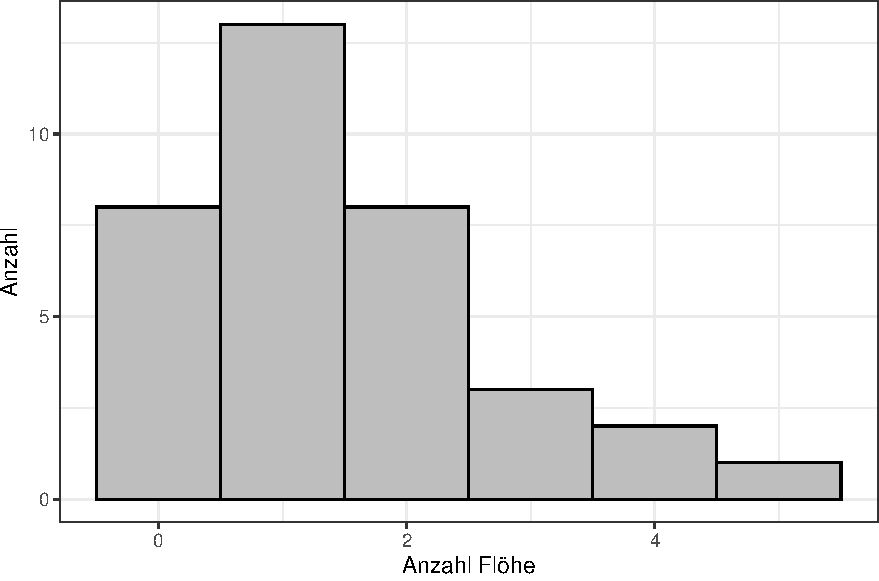
\includegraphics{./eda-ggplot_files/figure-pdf/fig-hist-flea-count-1.pdf}

}

\caption{\label{fig-hist-flea-count}Histogramm der Anzahl von Flöhen auf
39 Hunden.}

\end{figure}

Was sehen wir in der Abbildung~\ref{fig-hist-flea-count}? Anstatt von
gestapelten Punkten sehen wir jetzt Balken, die die jeweilige Anzahl an
Flöhen zusammenfassen. Der Unterschied ist bei einer diskreten Variable
wie der Anzahl (eng. \emph{count}) relativ gering.

Anders sieht es für kontenuierliche Variablen mit Kommazahlen aus.
Schauen wir uns das Gewicht der Flöhe an, so sehen wir, dass es sehr
viele Zahlen gibt, die nur einmal vorkomen.
Abbildung~\ref{fig-hist-flea-1} zeigt das Histogramm für das Geicht der
Flöhe.

\begin{Shaded}
\begin{Highlighting}[]
\FunctionTok{ggplot}\NormalTok{(}\AttributeTok{data =}\NormalTok{ dog\_fleas\_hist\_tbl, }\FunctionTok{aes}\NormalTok{(}\AttributeTok{x =}\NormalTok{ flea\_weight)) }\SpecialCharTok{+}
  \FunctionTok{geom\_histogram}\NormalTok{(}\AttributeTok{binwidth =} \DecValTok{1}\NormalTok{, }\AttributeTok{fill =} \StringTok{"gray"}\NormalTok{, }\AttributeTok{color =} \StringTok{"black"}\NormalTok{) }\SpecialCharTok{+}
  \FunctionTok{theme\_bw}\NormalTok{() }\SpecialCharTok{+}
  \FunctionTok{labs}\NormalTok{(}\AttributeTok{x =} \StringTok{"Gewicht [mg]"}\NormalTok{, }\AttributeTok{y =} \StringTok{"Anzahl"}\NormalTok{) }
\end{Highlighting}
\end{Shaded}

\begin{figure}[H]

{\centering 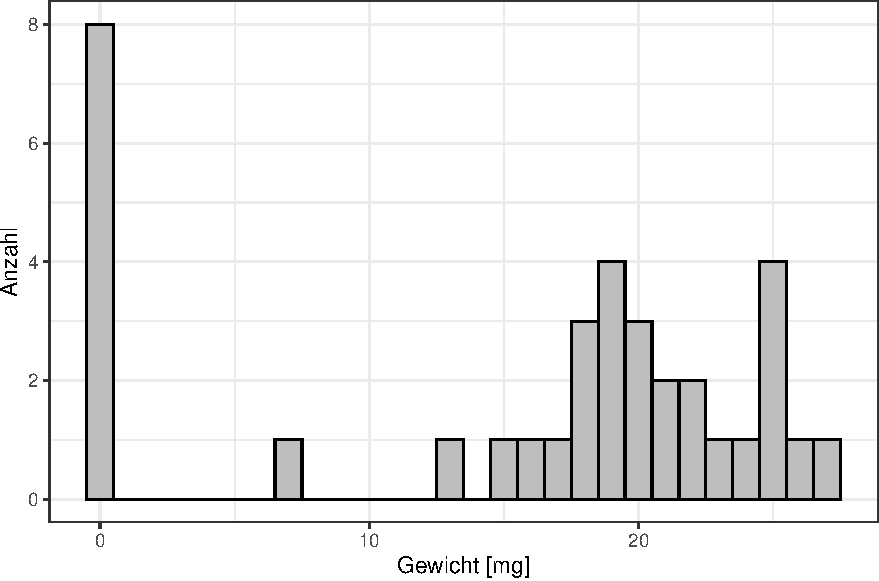
\includegraphics{./eda-ggplot_files/figure-pdf/fig-hist-flea-1-1.pdf}

}

\caption{\label{fig-hist-flea-1}Histogramm des Gewichts von Flöhen auf
39 Hunden.}

\end{figure}

Wie entsteht nun ein Hisotgramm für konetnierliche Zahlen? Schauen wir
uns dafür einmal ein kleineres Datenbeispiel an, in dem wir nur Flöhe
mit einem Gewicht größer als 11 und kleiner als 19 wäheln. Wir nutzen
dazu die Funktion
\texttt{filter(flea\_weight\ \textgreater{}\ 11\ \&\ flea\_weight\ \textless{}\ 19)}.
Wir erhalten folgende Zahlen und das entsprechende Histogramm.

\begin{verbatim}
[1] 13.29 14.91 15.64 16.58 17.66 17.81 18.40 18.64
\end{verbatim}

\begin{figure}

{\centering 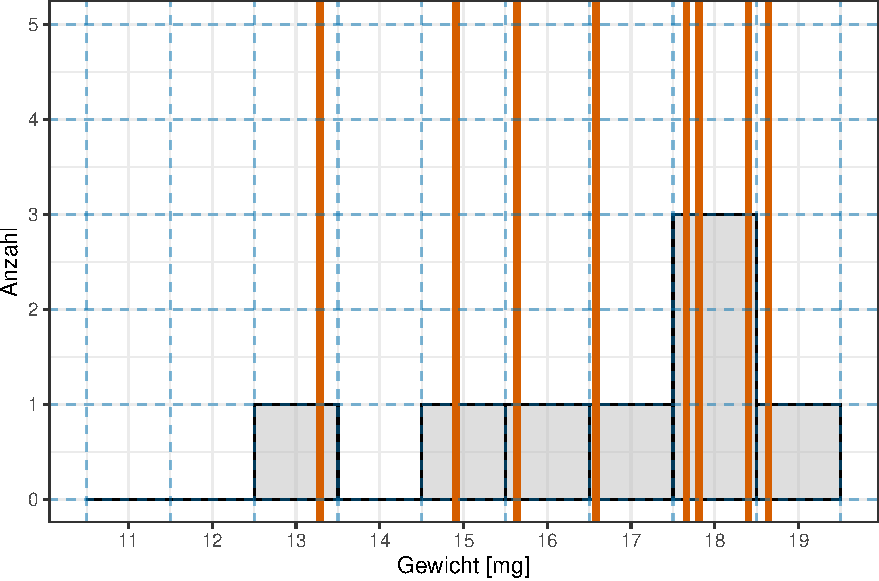
\includegraphics{./eda-ggplot_files/figure-pdf/fig-hist-flea-2-1.pdf}

}

\caption{\label{fig-hist-flea-2}Zusammenhang zwischen den einzelnen
Beobachtungen und der Höhe der einzelnen Balken am Beispiel von acht
Hunden.}

\end{figure}

Abbildung~\ref{fig-hist-flea-2} zeigt das Histogramm der reduzierten
Daten. Die roten vertikalen Linien zeigen die Position der einzelnen
Flohgewichte auf der x-Achse. Die blauen Hilfslinien machen nochmal
klarer, wie hoch die einzelnen Balken sind sowie welche Beobachtungen
auf der x-Achse in den jeweiligen Balken mit eingehen. Wir sehen, dass
wir einen Hund mit Flöhen haben, die zwischen 12.5 und 13.5 wiegen - der
entsprechende Balken erhält die Anzahl von eins. Auf der anderen Seite
sehen wir, dass es drei Hunde mit Flöhen, die zwischen 17.5 und 18.5
wiegen. Daher wächst der Balken auf eine Anzahl von drei.

Wir können mit der Option \texttt{binwidth} in dem
\texttt{geom\_histogram()} einstellen, wie breit auf der x-Achse die
jeweiligen Balken sein sollen. Hier empfiehlt es sich verschiedene
Zahlen für \texttt{binwidth}auszuprobieren.

\hypertarget{density-plot}{%
\subsection{Density Plot}\label{density-plot}}

Eine weitere Möglichkeit sich eine Verteilung anzuschauen, ist die Daten
nicht als Balkendiagramm sondern als Densityplot - also Dichteverteilung
- anzusehen. Im Prinzip verwandeln wir die Balken in eine Kurve. Damit
würden wir im Prinzip unterschiedliche Balkenhöhen ausgleichen udn eine
``glattere'' Darstellung erreichen. Wir wir aber gleich sehen werden,
benötigen wir dazu eine Menge an Beoabchtungen und auch dann ist das
Ergebnis eventuell nicht gut zu interpretieren.

\begin{Shaded}
\begin{Highlighting}[]
\FunctionTok{ggplot}\NormalTok{(}\AttributeTok{data =}\NormalTok{ dog\_fleas\_hist\_tbl, }\FunctionTok{aes}\NormalTok{(}\AttributeTok{x =}\NormalTok{ flea\_count)) }\SpecialCharTok{+}
  \FunctionTok{geom\_histogram}\NormalTok{(}\AttributeTok{binwidth =} \DecValTok{1}\NormalTok{, }\AttributeTok{fill =} \StringTok{"gray"}\NormalTok{, }\AttributeTok{color =} \StringTok{"black"}\NormalTok{) }\SpecialCharTok{+}
  \FunctionTok{theme\_bw}\NormalTok{() }\SpecialCharTok{+}
  \FunctionTok{labs}\NormalTok{(}\AttributeTok{x =} \StringTok{"Anzahl Flöhe"}\NormalTok{, }\AttributeTok{y =} \StringTok{"Anzahl"}\NormalTok{)}

\FunctionTok{ggplot}\NormalTok{(}\AttributeTok{data =}\NormalTok{ dog\_fleas\_hist\_tbl, }\FunctionTok{aes}\NormalTok{(}\AttributeTok{x =}\NormalTok{ flea\_count)) }\SpecialCharTok{+}
  \FunctionTok{geom\_density}\NormalTok{(}\AttributeTok{fill =} \StringTok{"gray"}\NormalTok{, }\AttributeTok{color =} \StringTok{"black"}\NormalTok{) }\SpecialCharTok{+}
  \FunctionTok{theme\_bw}\NormalTok{() }\SpecialCharTok{+}
  \FunctionTok{labs}\NormalTok{(}\AttributeTok{x =} \StringTok{"Anzahl Flöhe"}\NormalTok{, }\AttributeTok{y =} \StringTok{"Häufigkeit"}\NormalTok{) }
\end{Highlighting}
\end{Shaded}

\begin{figure*}

\begin{minipage}[t]{0.50\linewidth}

{\centering 

\raisebox{-\height}{

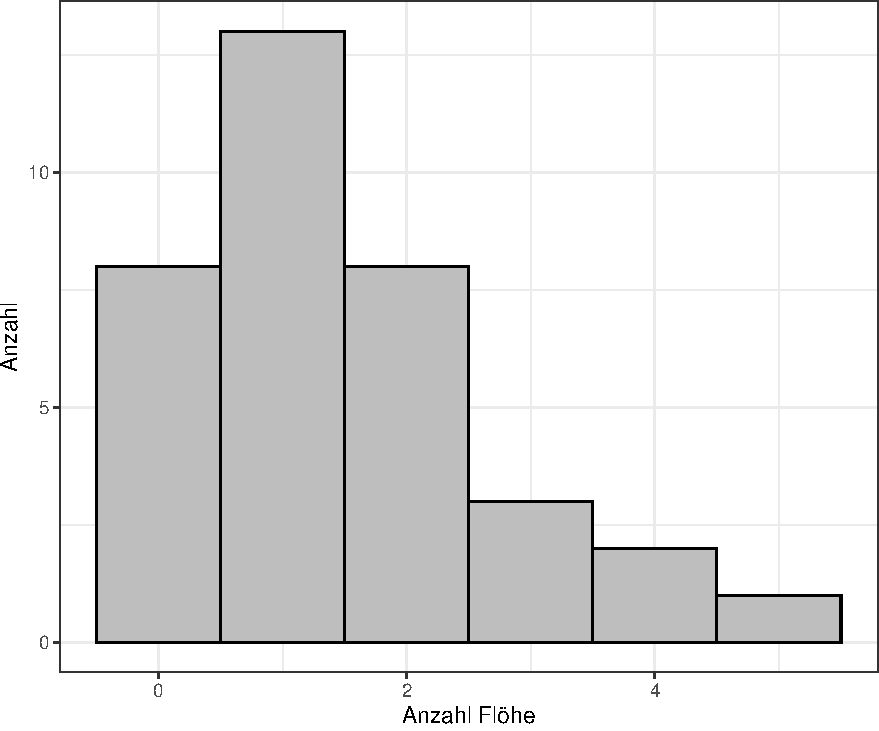
\includegraphics{./eda-ggplot_files/figure-pdf/fig-dens-flea-1-1.pdf}

}

}

\subcaption{\label{fig-dens-flea-1-1}Histogramm}
\end{minipage}%
%
\begin{minipage}[t]{0.50\linewidth}

{\centering 

\raisebox{-\height}{

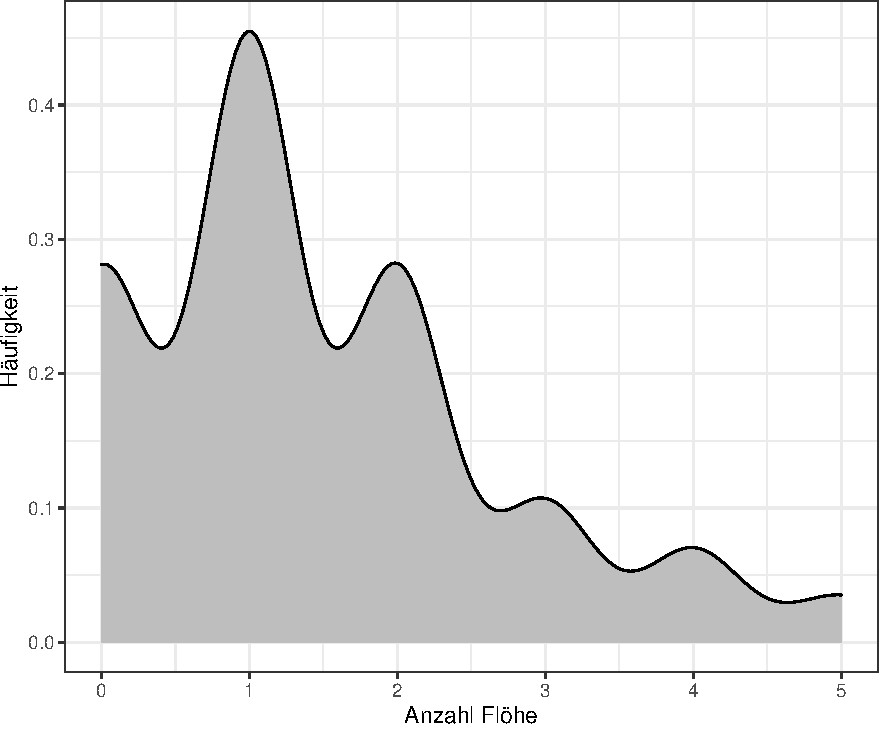
\includegraphics{./eda-ggplot_files/figure-pdf/fig-dens-flea-1-2.pdf}

}

}

\subcaption{\label{fig-dens-flea-1-2}Densityplot}
\end{minipage}%

\caption{\label{fig-dens-flea-1}Zusammenhang von Histogramm und
Densityplot an der Anzahl der Flöhe auf 39 Hunden.}

\end{figure*}

Abbildung~\ref{fig-dens-flea-1} zeigt auf der linken Seite erneut die
Abbildung des Histogramms als Balkendiagramm für die Anzahl der Flöhe
auf den 39 Hunden. Auf der rechten Seite die entsprechenden gleichen
Daten als Denistyplot. Klar ist die Wellenbewegung des Densityplots zu
erkennen. Hier leigen zu wenige Beobachtungen und Kategorien auf der
x-Achse vor, so dass der Densityplot nicht zu empfehlen ist.

\begin{Shaded}
\begin{Highlighting}[]
\FunctionTok{ggplot}\NormalTok{(}\AttributeTok{data =}\NormalTok{ dog\_fleas\_hist\_tbl, }\FunctionTok{aes}\NormalTok{(}\AttributeTok{x =}\NormalTok{ flea\_weight)) }\SpecialCharTok{+}
  \FunctionTok{geom\_histogram}\NormalTok{(}\AttributeTok{binwidth =} \DecValTok{1}\NormalTok{, }\AttributeTok{fill =} \StringTok{"gray"}\NormalTok{, }\AttributeTok{color =} \StringTok{"black"}\NormalTok{) }\SpecialCharTok{+}
  \FunctionTok{theme\_bw}\NormalTok{() }\SpecialCharTok{+}
  \FunctionTok{labs}\NormalTok{(}\AttributeTok{x =} \StringTok{"Gewicht [mg]"}\NormalTok{, }\AttributeTok{y =} \StringTok{"Anzahl"}\NormalTok{) }

\FunctionTok{ggplot}\NormalTok{(}\AttributeTok{data =}\NormalTok{ dog\_fleas\_hist\_tbl, }\FunctionTok{aes}\NormalTok{(}\AttributeTok{x =}\NormalTok{ flea\_weight)) }\SpecialCharTok{+}
  \FunctionTok{geom\_density}\NormalTok{(}\AttributeTok{fill =} \StringTok{"gray"}\NormalTok{, }\AttributeTok{color =} \StringTok{"black"}\NormalTok{) }\SpecialCharTok{+}
  \FunctionTok{theme\_bw}\NormalTok{() }\SpecialCharTok{+}
  \FunctionTok{labs}\NormalTok{(}\AttributeTok{x =} \StringTok{"Gewicht [mg]"}\NormalTok{, }\AttributeTok{y =} \StringTok{"Häufigkeit"}\NormalTok{) }
\end{Highlighting}
\end{Shaded}

\begin{figure*}

\begin{minipage}[t]{0.50\linewidth}

{\centering 

\raisebox{-\height}{

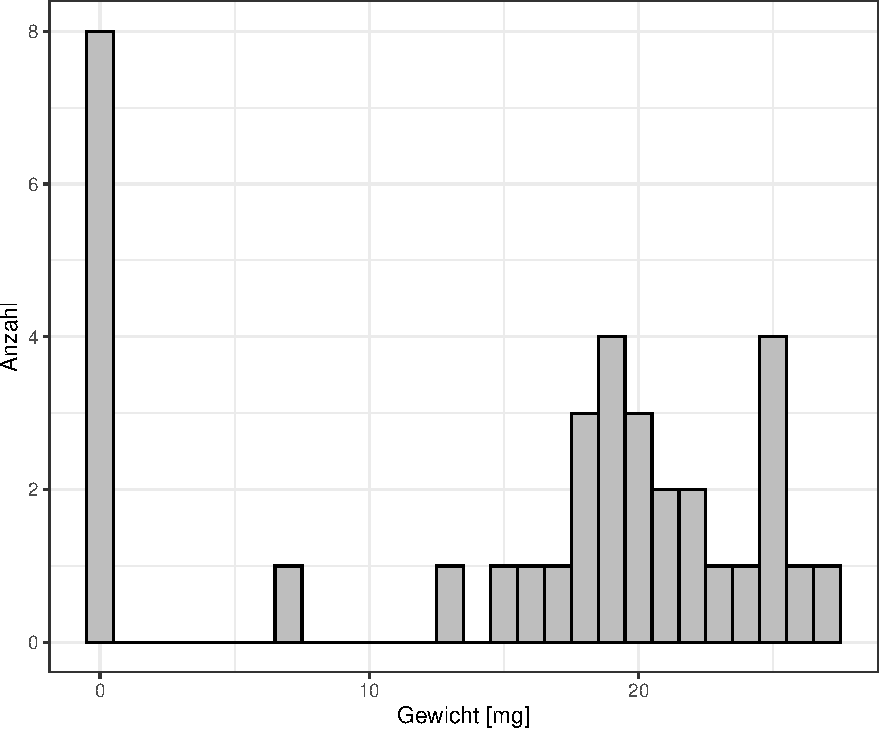
\includegraphics{./eda-ggplot_files/figure-pdf/fig-dens-flea-2-1.pdf}

}

}

\subcaption{\label{fig-dens-flea-2-1}Histogramm}
\end{minipage}%
%
\begin{minipage}[t]{0.50\linewidth}

{\centering 

\raisebox{-\height}{

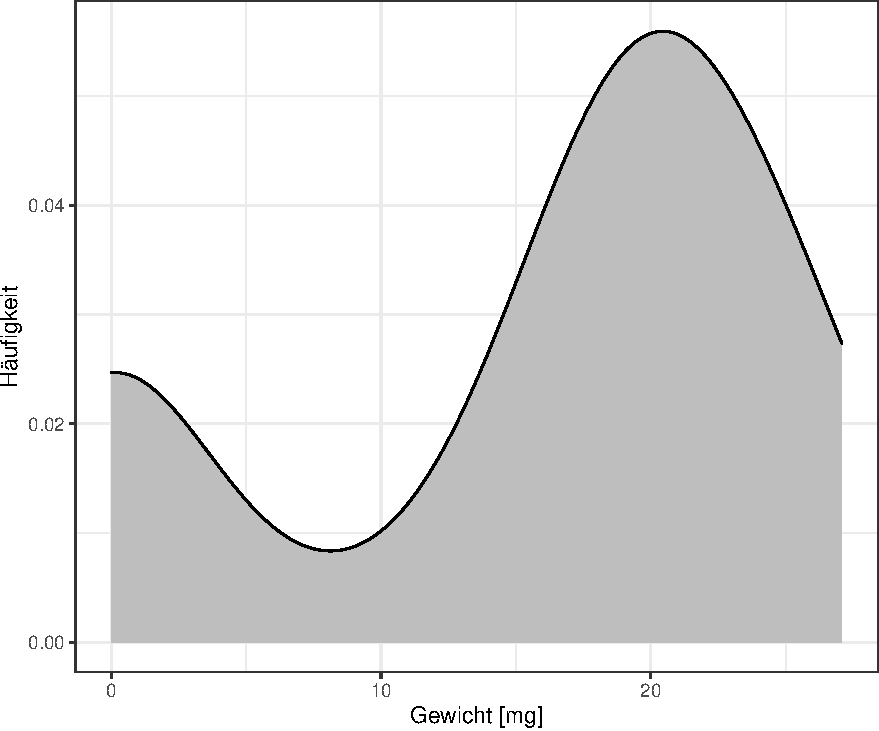
\includegraphics{./eda-ggplot_files/figure-pdf/fig-dens-flea-2-2.pdf}

}

}

\subcaption{\label{fig-dens-flea-2-2}Densityplot}
\end{minipage}%

\caption{\label{fig-dens-flea-2}Zusammenhang von Histogramm und
Densityplot am Gewicht der Flöhe auf 39 Hunden.}

\end{figure*}

Abbildung~\ref{fig-dens-flea-2} zeigt auf der linken Seite erneut die
Abbildung des Histogramms als Balkendiagramm für das Gewicht der Flöhe
auf den 39 Hunden. Insbesondere bei dieser Abbildung erkennst du die
Nachteile des Densityplot. Dadurch das es einen Peak von acht Hunden mit
einem Flohgewicht von 0 gibt, zeigt der Densityplot eine seltsame
Wellenform. Es emppfielt sich daher die Daten zuerst als Histogramm zu
betrachten.

\hypertarget{sec-eda-boxplot}{%
\subsection{Boxplot}\label{sec-eda-boxplot}}

In Kapitel~\ref{sec-desc-stat} haben wir den Median und die Quartile
kennengelernt. Mit dem Boxplot können wir den Median und die Quartile
visualisieren. In Abbildung~\ref{fig-boxplot-drawn} sehen wir einen
Boxplot, der den Median und die Quartile visualisiert. Die Box wird aus
dem IQR gebildet. Der Median wird als Strich in der Box gezeigt. Die
Schnurrhaare (eng. \emph{Whiskers}) sind das 1.5 fache des IQR. Punkte
die außerhalb der Schnurrhaare liegen werden als einzelne Punkte
dargestellt. Diese einzelnen Punkte werden auch als Ausreißer (eng.
\emph{Outlier}) bezeichnet.

\begin{figure*}

{\centering 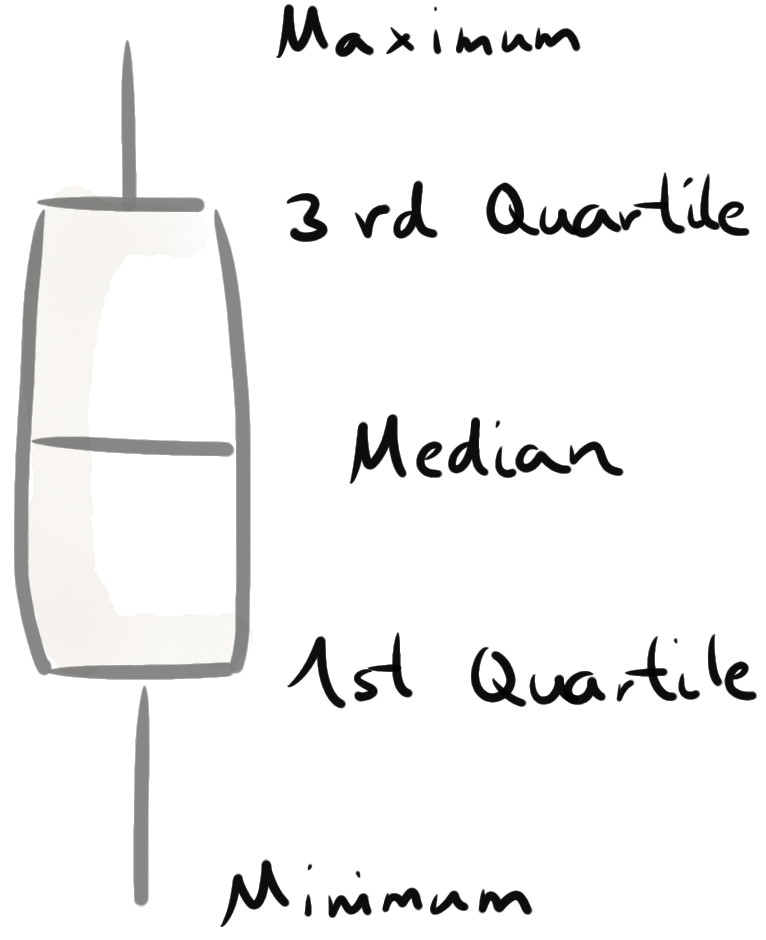
\includegraphics[width=1\textwidth,height=\textheight]{./images/boxplot-drawn.png}

}

\caption{\label{fig-boxplot-drawn}Ein Boxplot der die statistischen
Maßzahlen Median und Quartile visualisiert. Die Box wird aus dem IQR
gebildet. Der Median wird als Strich in der Box gezeigt. Die
Schnurrhaare sind das 1.5 fache des IQR. Punkte die außerhalb der
Schnurrhaare liegen werden als einzele Punkte dargestellt.}

\end{figure*}

In Abbildung~\ref{fig-boxplot-drawn-distribution} sehen wir den
Zusammenhang zwischen einem Histogramm, Densityplot und dem Boxplot. Der
Median \(\tilde{y}\) im Boxplot zeigt die höchste Stelle des
Densityplots an. Durch einen Boxplot kann die Verteilung der
entsprechenden Zahlen abgeschätzt werden.

\begin{figure}

{\centering 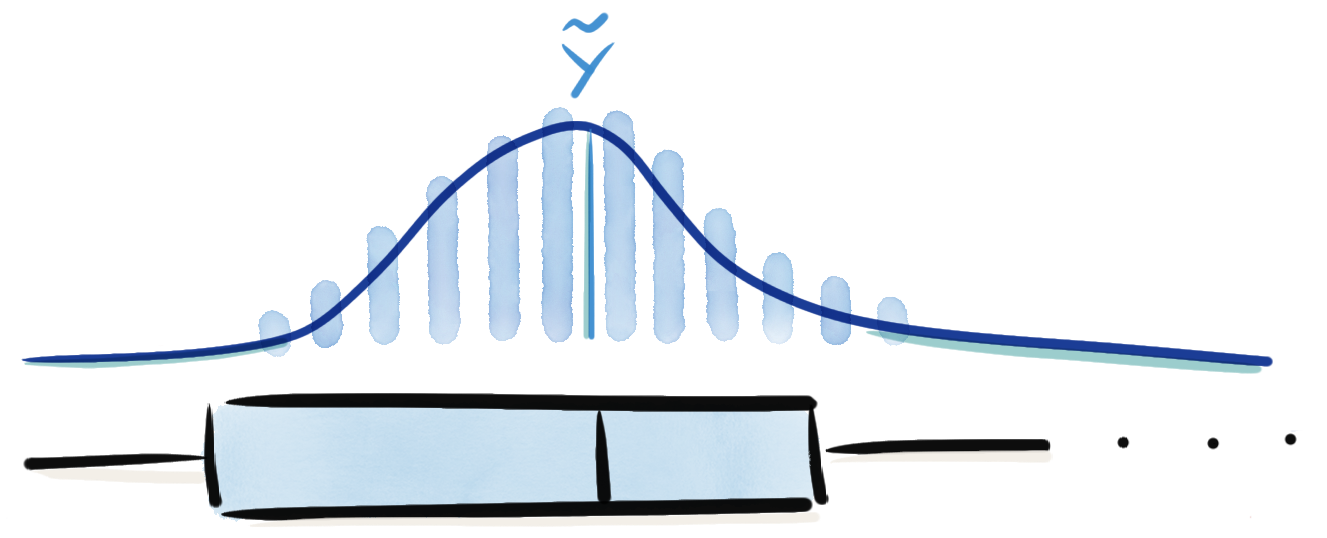
\includegraphics[width=1\textwidth,height=\textheight]{./images/boxplot-drawn-distribution.png}

}

\caption{\label{fig-boxplot-drawn-distribution}Der Zusammenhang von
Histogram, Densityplot und Boxplot.}

\end{figure}

Die ``liegende'' Darstellung des Boxplots dient nur der
Veranschaulichung und dem Verständnis des Zusammenhangs von Histogramm
und Boxplot. In der Abbildung~\ref{fig-boxplot-drawn-flipped} sehen wir
drei Boxplots für einen Faktor mit drei Leveln. Jedes Level wird duch
einen Boxplot dargestellt. Zum Beispiel eine Düngerbehandlung mit drei
Konzentrationen. Auf der x-Achse würden wir die Behandelung finden und
auf der y-Achse das Trockengewicht in {[}kg/ha{]}.

\begin{figure}

{\centering 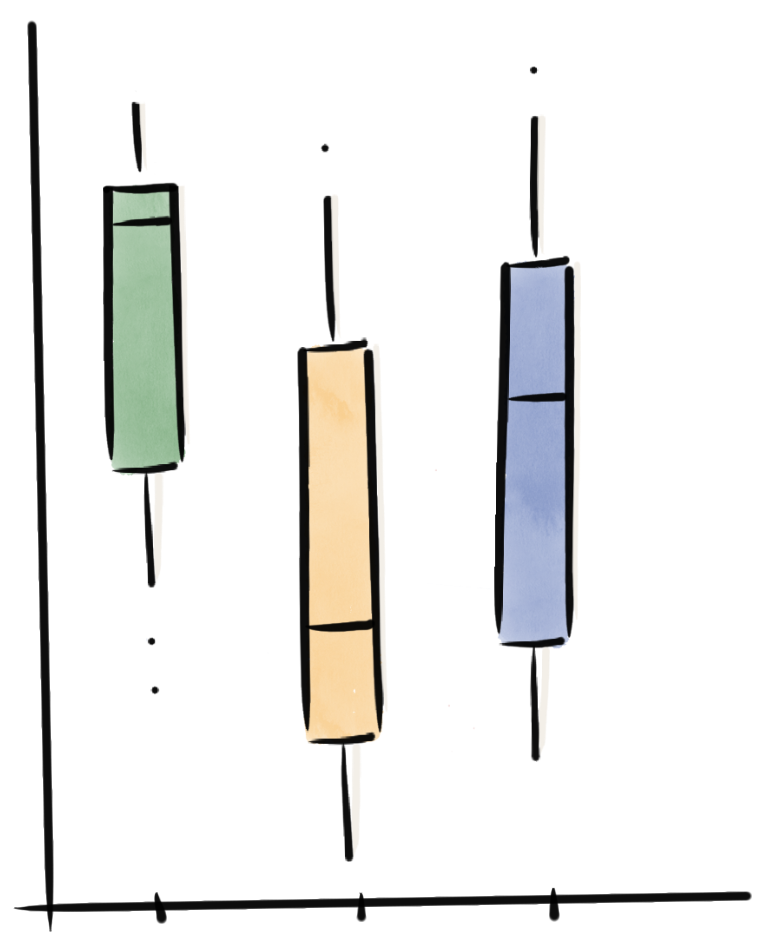
\includegraphics[width=0.6\textwidth,height=\textheight]{./images/boxplot-drawn-flipped.png}

}

\caption{\label{fig-boxplot-drawn-flipped}Typische Darstellung von drei
Gruppen jeweils dargestellt durch einen Boxplot. Boxplots werden in der
Anwendung stehtend dargestellt. Insbesondere wenn die Boxplots mehrere
Gruppen repräsentieren.}

\end{figure}

Wie erstellen wir nun einen Boxplot in R? Zuerst laden wir die Daten mit
der Funktion \texttt{read\_excel()} in R, wenn du die Daten als
\texttt{.xlsx} Datei vorliegen hast. Im XX kannst du nochmal das
Importieren von Daten wiederholen.

\begin{Shaded}
\begin{Highlighting}[]
\NormalTok{flea\_dog\_cat\_tbl }\OtherTok{\textless{}{-}} \FunctionTok{read\_excel}\NormalTok{(}\StringTok{"data/flea\_dog\_cat.xlsx"}\NormalTok{)}
\end{Highlighting}
\end{Shaded}

\begin{figure}

{\centering 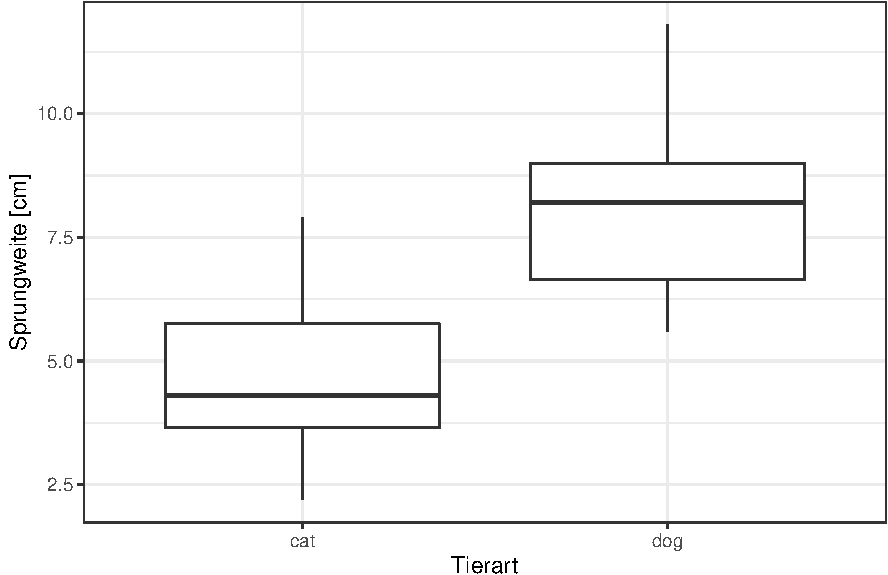
\includegraphics{./eda-ggplot_files/figure-pdf/fig-boxplot-flea-0-1.pdf}

}

\caption{\label{fig-boxplot-flea-0}An 39 Hunden wurde die Anzahl an
Flöhen gezählt.}

\end{figure}

In Abbildung~\ref{fig-boxplot-flea-0} ist der Boxplot für die Daten aus
der Datei \texttt{flea\_dog\_cat.xlsx} dargestellt. Auf der x-Achse
finden wir die Tierart als \texttt{cat} und \texttt{dog}. Auf der
y-Achse ist die Sprungweite in {[}cm{]} dargestellt.

Wir erkennen auf einen Blick, dass die Sprungweite von den Hundeflöhen
weiter ist als die Sprungweite der Katzenflöhe. Im Weiteren können wir
abschätzen, dass die Streuung etwa gleich groß ist. Die Boxen sind in
etwa gleich groß und die Whiskers in etwa gleich lang.

\begin{Shaded}
\begin{Highlighting}[]
\FunctionTok{ggplot}\NormalTok{(}\AttributeTok{data =}\NormalTok{ flea\_dog\_cat\_tbl, }\FunctionTok{aes}\NormalTok{(}\AttributeTok{x =}\NormalTok{ animal, }\AttributeTok{y =}\NormalTok{ jump\_length,}
                                    \AttributeTok{fill =}\NormalTok{ animal)) }\SpecialCharTok{+}
  \FunctionTok{geom\_boxplot}\NormalTok{() }\SpecialCharTok{+}
  \FunctionTok{geom\_jitter}\NormalTok{(}\AttributeTok{width =} \FloatTok{0.25}\NormalTok{, }\AttributeTok{shape =} \DecValTok{1}\NormalTok{) }\SpecialCharTok{+}
  \FunctionTok{theme\_bw}\NormalTok{() }\SpecialCharTok{+}
  \FunctionTok{labs}\NormalTok{(}\AttributeTok{x =} \StringTok{"Tierart"}\NormalTok{, }\AttributeTok{y =} \StringTok{"Sprungweite [cm]"}\NormalTok{) }
\end{Highlighting}
\end{Shaded}

\begin{figure}[H]

{\centering 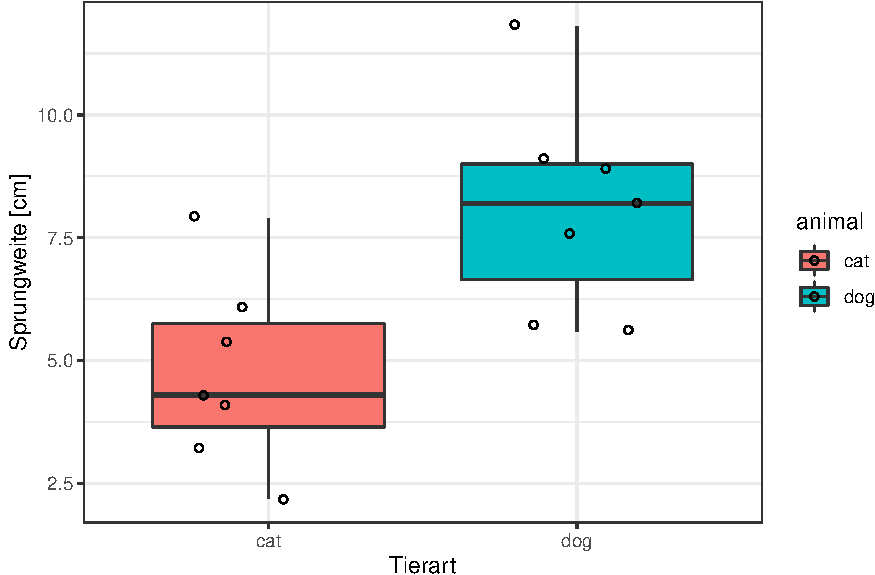
\includegraphics{./eda-ggplot_files/figure-pdf/fig-boxplot-freshmatter-2-1.pdf}

}

\caption{\label{fig-boxplot-freshmatter-2}An 39 Hunden wurde die Anzahl
an Flöhen gezählt.}

\end{figure}

Wir neigen dazu die Boxplots überzuinterpretieren, wenn die Anzahl der
Beobachtungen klein ist. Deshalb können wir mit dem
\texttt{geom\_jitter()} noch die Beobachtungen zu den Boxplot ergänzen,
dargestellt in Abbildung~\ref{fig-boxplot-freshmatter-2}. Die Funktion
\texttt{geom\_jitter()} streut die Punkte zufällig, so dass keine Punkte
übereinanderliegen. Wir haben hier die Streuuweite durch die Option
\texttt{width\ =\ 0.25} etwas eingeschränkt. Darüber hinaus habe wir das
Aussehen der Punkte mit \texttt{shape\ =\ 1} geändert, so dass wir die
Jitter-Punkte von den potenziellen Ausreißer-Punkten unterscheiden
können. Du kannst auch andere Zahlen hinter \texttt{shape} eintragen um
verschiedene Punktesymbole durchzuprobieren. Eine Übersicht an
\texttt{shapes} findest du auch hier unter
\href{http://www.cookbook-r.com/Graphs/Shapes_and_line_types/}{Cookbook
for R \textgreater{} Graphs \textgreater{} Shapes and line types}.

\hypertarget{sec-eda-barplot}{%
\subsection{Barplot oder Balkendiagramm}\label{sec-eda-barplot}}

Der Barplot oder das Balkendiagramm ist eigentlich veraltet. Wir haben
mit dem Boxplot eine viel bessere Methode um eine Verteilung und
\emph{gleichzeitig} auch die Gruppenunterschiede zu visualisieren. Warum
nutzen wir jetzt so viel den Braplot? Das hat damit zu tun, dass früher
- oder besser bis vor kurzem - in Excel kein Boxplot möglich war. Daher
nutzte jeder der mit Excel seine Daten auswertet den Barplot. Und was
der Bauer nicht kennt\ldots{}

\marginnote{\begin{footnotesize}

\begin{enumerate}
\def\labelenumi{\arabic{enumi}.}
\tightlist
\item
  Alles was es schon gab, als Du geboren wurdest, ist normal und
  gewöhnlich. Diese Dinge werden als natürlich wahrgenommen und halten
  die Welt am Laufen.
\item
  Alles was zwischen Deinem 16ten und 36ten Lebensjahr erfunden wird ist
  neu, aufregend und revoltionär. Und vermutlich kannst Du in dem
  Bereich sogar Karriere machen.
\item
  Alles was nach dem 36ten Lebensjahr erfunden wird ist gegen die
  natürliche Ordnung der Dinge.
\end{enumerate}

-- Douglas Adams aus \emph{Per Anhalter durch die Galaxis}

\end{footnotesize}}

Deshalb ist hier auch der Barplot dargestellt. Ich persönlich mag den
Barplot übrhaupt nicht. Der Barplot ist einfach schlechter als der
Boxplot. Aber gut, häufog musst du den Barplot in deiner Abschlussarbeit
machen. Also dann hier der Barplot.

Wie erstellen wir nun einen Barplot in R? Zuerst laden wir die Daten mit
der Funktion \texttt{read\_excel()} in R, wenn du die Daten als
\texttt{.xlsx} Datei vorliegen hast. Im
Kapitel~\ref{sec-programming-import} kannst du nochmal das Importieren
von Daten wiederholen.

\begin{Shaded}
\begin{Highlighting}[]
\NormalTok{flea\_dog\_cat\_tbl }\OtherTok{\textless{}{-}} \FunctionTok{read\_excel}\NormalTok{(}\StringTok{"data/flea\_dog\_cat.xlsx"}\NormalTok{)}
\end{Highlighting}
\end{Shaded}

Wir müssen jetzt für \texttt{ggplot()} noch den Mittelwert und die
Streuung für die Gruppen berechnen. Ein komplexeres Beispiel für einen
Barplot findets du in Kapitel~\ref{sec-beispiel-auswertung}. Du kanst
als Streuung die Standardabweichung oder den Standardfehler nehmen. Ich
würde die Standardabweichung bei kleinen Fallzahlen kleiner als 20
Beobachtungen nehmen.

\begin{Shaded}
\begin{Highlighting}[]
\NormalTok{stat\_tbl }\OtherTok{\textless{}{-}}\NormalTok{ flea\_dog\_cat\_tbl }\SpecialCharTok{\%\textgreater{}\%} 
  \FunctionTok{group\_by}\NormalTok{(animal) }\SpecialCharTok{\%\textgreater{}\%} 
  \FunctionTok{summarise}\NormalTok{(}\AttributeTok{mean =} \FunctionTok{mean}\NormalTok{(jump\_length),}
            \AttributeTok{sd =} \FunctionTok{sd}\NormalTok{(jump\_length),}
            \AttributeTok{se =}\NormalTok{ sd}\SpecialCharTok{/}\FunctionTok{sqrt}\NormalTok{(}\FunctionTok{n}\NormalTok{()))}
\end{Highlighting}
\end{Shaded}

Wir nutzen nun das Objekt \texttt{stat\_tbl} um den Barplot mit der
Funktion \texttt{ggplot()} zu erstellen. Dabei müssen wir zum einen
schauen, dass die Balken nicht übereinander angeordnet sind.
Nebeneinander angeordnete Balken kriegen wir mit der Option
\texttt{stat\ =\ "identity"} in dem \texttt{geom\_bar()}. Dann müssen
wir noch die Fehlerbalken ergänzen mit dem \texttt{geom\_errorbar}. Hier
kann nochmal mit der Option \texttt{width\ =} an der Länge der
Fehlerenden gedreht werden.

\begin{Shaded}
\begin{Highlighting}[]
\FunctionTok{ggplot}\NormalTok{(stat\_tbl, }\FunctionTok{aes}\NormalTok{(}\AttributeTok{x =}\NormalTok{ animal, }\AttributeTok{y =}\NormalTok{ mean, }\AttributeTok{fill =}\NormalTok{ animal)) }\SpecialCharTok{+} 
    \FunctionTok{geom\_bar}\NormalTok{(}\AttributeTok{stat =} \StringTok{"identity"}\NormalTok{) }\SpecialCharTok{+}
    \FunctionTok{geom\_errorbar}\NormalTok{(}\FunctionTok{aes}\NormalTok{(}\AttributeTok{ymin =}\NormalTok{ mean}\SpecialCharTok{{-}}\NormalTok{sd, }\AttributeTok{ymax =}\NormalTok{ mean}\SpecialCharTok{+}\NormalTok{sd),}
                  \AttributeTok{width =} \FloatTok{0.2}\NormalTok{)}
\end{Highlighting}
\end{Shaded}

\begin{figure}[H]

{\centering 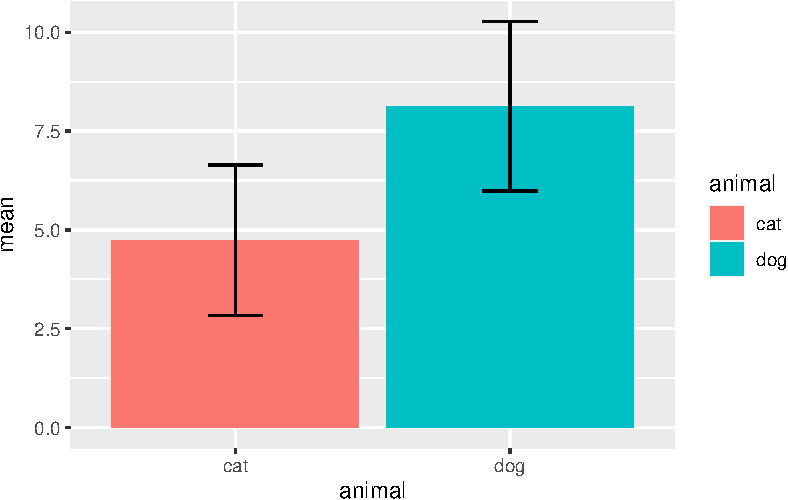
\includegraphics{./eda-ggplot_files/figure-pdf/unnamed-chunk-20-1.pdf}

}

\end{figure}

Im Zweifel muss du nochmal googlen und schauen welche Form dir am besten
zusgat. Es gibt sehr viele Möglichkeiten einen Barplot zu erstellen.
Daher komm im Zweifel einmal ins R Tutorium.

\hypertarget{sec-eda-dotplot}{%
\subsection{Dotplot}\label{sec-eda-dotplot}}

Wenn wir weniger als fünf Beobachtungen haben, dann ist meist ein
Boxplot verzerrend. Wir sehen eine Box und glauben, dass wir viele
Datenpunkte vorliegen haben. Bei 3 bis 7 Beobachtungen je Gruppe bietet
sich der Dotplot als eine Lösung an. Wir stellen hier alle Beobachtungen
als einzelne Punkte dar.

Wie erstellen wir nun einen Dotplot in R? Zuerst laden wir die Daten mit
der Funktion \texttt{read\_excel()} in R, wenn du die Daten als
\texttt{.xlsx} Datei vorliegen hast. Im XX kannst du nochmal das
Importieren von Daten wiederholen.

\begin{Shaded}
\begin{Highlighting}[]
\NormalTok{flea\_dog\_cat\_tbl }\OtherTok{\textless{}{-}} \FunctionTok{read\_excel}\NormalTok{(}\StringTok{"data/flea\_dog\_cat.xlsx"}\NormalTok{)}
\end{Highlighting}
\end{Shaded}

\begin{Shaded}
\begin{Highlighting}[]
\FunctionTok{ggplot}\NormalTok{(}\AttributeTok{data =}\NormalTok{ flea\_dog\_cat\_tbl, }\FunctionTok{aes}\NormalTok{(}\AttributeTok{x =}\NormalTok{ animal, }\AttributeTok{y =}\NormalTok{ grade,}
                                    \AttributeTok{fill =}\NormalTok{ animal)) }\SpecialCharTok{+}
  \FunctionTok{geom\_dotplot}\NormalTok{(}\AttributeTok{binaxis =} \StringTok{"y"}\NormalTok{, }\AttributeTok{stackdir =} \StringTok{"center"}\NormalTok{) }\SpecialCharTok{+}
  \FunctionTok{theme\_bw}\NormalTok{() }\SpecialCharTok{+}
  \FunctionTok{labs}\NormalTok{(}\AttributeTok{x =} \StringTok{"Tierart"}\NormalTok{, }\AttributeTok{y =} \StringTok{"Boniturnote [1{-}9]"}\NormalTok{) }
\end{Highlighting}
\end{Shaded}

\begin{figure}[H]

{\centering 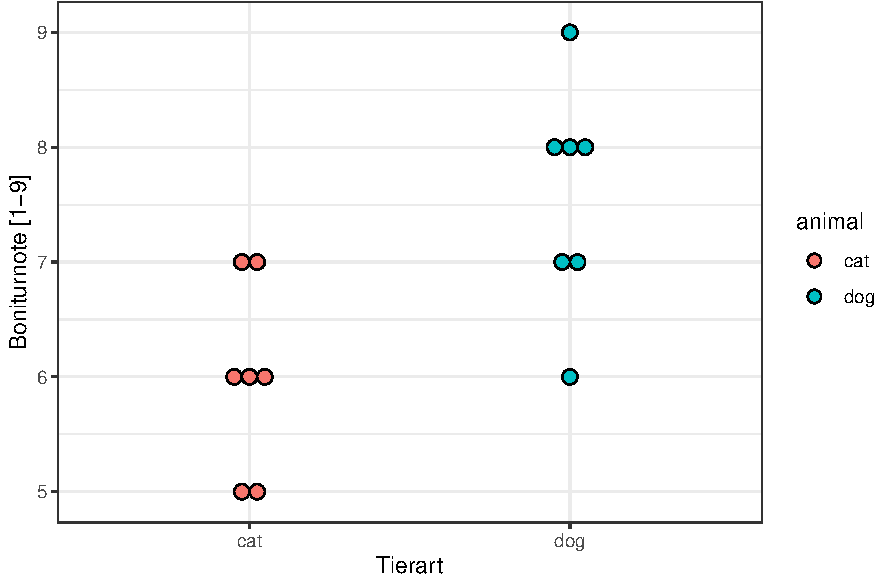
\includegraphics{./eda-ggplot_files/figure-pdf/fig-dotplot-flea-eda-0-1.pdf}

}

\caption{\label{fig-dotplot-flea-eda-0}Der Dotplot für die Anzahl der
Flöhe für die beiden Tierarten Hund und Katze.}

\end{figure}

In Abbildung~\ref{fig-dotplot-flea-eda-0} sehen wir den Dotplot aus der
Datei \texttt{flea\_dog\_cat.xlsx}. Auf der x-Achse sind die Level des
Faktors \texttt{animal} dargestellt und auf der y-Achse die
Notenbewertung \texttt{grade} der einzelnen Hunde und Katzen. Die
Funktion \texttt{geom\_dotplot()} erschafft das Layer für die Dots bzw.
Punkte. Wir müssen in der Funktion noch zwei Dinge angeben, damit der
Plot so aussieht, dass wir den Dotplot gut interpretieren können. Zum
einen müssen wir die Option \texttt{binaxis\ =\ y} wählen, damit die
Punkte horizontal geordent werden. Zum anderen wollen wir auch, dass die
Punkte zentriert sind und nutzen dafür die Option
\texttt{stackdir\ =\ center}.

\begin{Shaded}
\begin{Highlighting}[]
\FunctionTok{ggplot}\NormalTok{(}\AttributeTok{data =}\NormalTok{ flea\_dog\_cat\_tbl, }\FunctionTok{aes}\NormalTok{(}\AttributeTok{x =}\NormalTok{ animal, }\AttributeTok{y =}\NormalTok{ grade,}
                            \AttributeTok{fill =}\NormalTok{ animal)) }\SpecialCharTok{+}
  \FunctionTok{geom\_dotplot}\NormalTok{(}\AttributeTok{binaxis =} \StringTok{"y"}\NormalTok{, }\AttributeTok{stackdir =} \StringTok{"center"}\NormalTok{) }\SpecialCharTok{+}
  \FunctionTok{stat\_summary}\NormalTok{(}\AttributeTok{fun =}\NormalTok{ median, }\AttributeTok{fun.min =}\NormalTok{ median, }\AttributeTok{fun.max =}\NormalTok{ median,}
               \AttributeTok{geom =} \StringTok{"crossbar"}\NormalTok{, }\AttributeTok{width =} \FloatTok{0.5}\NormalTok{) }\SpecialCharTok{+}
  \FunctionTok{theme\_bw}\NormalTok{() }\SpecialCharTok{+}
  \FunctionTok{labs}\NormalTok{(}\AttributeTok{x =} \StringTok{"Tierart"}\NormalTok{, }\AttributeTok{y =} \StringTok{"Boniturnote [1{-}9]"}\NormalTok{) }
\end{Highlighting}
\end{Shaded}

\begin{figure}[H]

{\centering 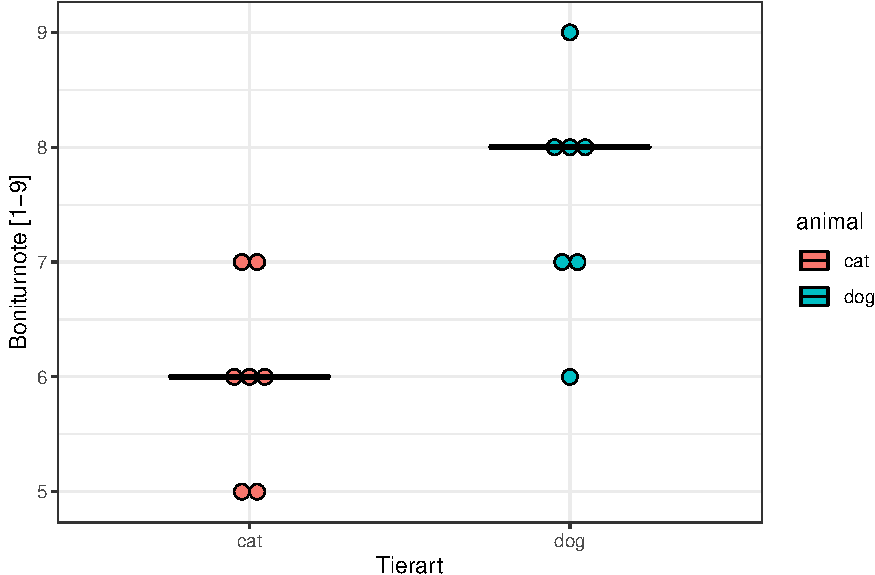
\includegraphics{./eda-ggplot_files/figure-pdf/fig-dotplot-flea-eda-1-1.pdf}

}

\caption{\label{fig-dotplot-flea-eda-1}Der Dotplot für die Anzahl der
Flöhe für die beiden Tierarten Hund und Katze. Die schwarze Linie stelt
den Median für die beiden Tierarten dar.}

\end{figure}

Nun macht es wenig Sinn bei sehr wenigen Beobachtungen noch statistische
Maßzahlen mit in den Plot zu zeichnen. Sonst hätten wir auch gleich
einen Boxplot als Visualisierung der Daten wählen können. In
Abbildung~\ref{fig-dotplot-flea-eda-1} sehen wir die Ergänzung des
Medians. Hier müssen wir etwas mehr angeben, aber immerhin haben wir so
eine Idee, wo die ``meisten'' Beobachtungen wären. Aber auch hier ist
Vorsicht geboten. Wir haben sehr wenige Beobachtungen, so dass eine
Beobachtung mehr oder weniger große Auswirkungen auf den Median und die
Interpretation hat.

\hypertarget{sec-eda-scatter}{%
\subsection{Scatterplot}\label{sec-eda-scatter}}

Der Scatterplot wird auch xy-Plot genannt. Wir stellen in einem
Scatterplot zwei kontenuierliche Variablen dar. Dann wollen wir eine
Linie durch die Punkte legen. Im Prinzip fragen wir uns, wie hänge die
Werte auf der y-Achse von den Werten auf der x-Achse ab? Wenn sich also
die Werte auf der x-Achse erhöhen, wie verhalten sich dann die Werte auf
der y-Achse?

\begin{Shaded}
\begin{Highlighting}[]
\FunctionTok{ggplot}\NormalTok{(}\AttributeTok{data =}\NormalTok{ flea\_dog\_cat\_tbl, }\FunctionTok{aes}\NormalTok{(}\AttributeTok{x =}\NormalTok{ flea\_count, }\AttributeTok{y =}\NormalTok{ jump\_length)) }\SpecialCharTok{+}
  \FunctionTok{geom\_point}\NormalTok{() }\SpecialCharTok{+}
  \FunctionTok{stat\_smooth}\NormalTok{(}\AttributeTok{method =} \StringTok{"lm"}\NormalTok{, }\AttributeTok{se =} \ConstantTok{FALSE}\NormalTok{) }\SpecialCharTok{+}
  \FunctionTok{theme\_bw}\NormalTok{() }\SpecialCharTok{+}
  \FunctionTok{labs}\NormalTok{(}\AttributeTok{x =} \StringTok{"Anzahl der Flöhe"}\NormalTok{, }\AttributeTok{y =} \StringTok{"Sprungweite in [cm]"}\NormalTok{) }
\end{Highlighting}
\end{Shaded}

\begin{figure}[H]

{\centering 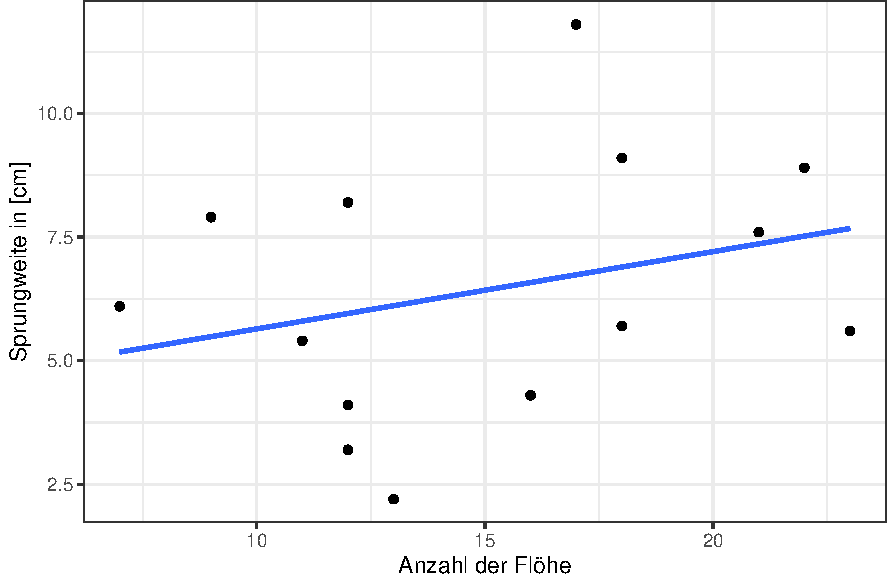
\includegraphics{./eda-ggplot_files/figure-pdf/fig-scatter-flea-0-1.pdf}

}

\caption{\label{fig-scatter-flea-0}Zusammenhang zwischen der Sprungweite
in {[}cm{]} und der Anzahl an Flöhen auf den 39 Hunden. Jeder Punkt
stellt einen Hund dar.}

\end{figure}

Abbildung~\ref{fig-scatter-flea-0} zeigt den Scatterplot für die Spalte
\texttt{flea\_count} auf der x-Achse und \texttt{jump\_length} auf der
y-Achse. Mit der Funktion \texttt{geom\_point()} können wir die
Punktepaare für jede Beobachtung zeichnen. In unserem Fall zeichnen wir
mit der Funktion \texttt{stat\_smooth()} noch die entsprechende Grade
durch die Punkte. Es handelt sich hierbei um eine Regression. Du kannst
im Kapitel XX mehr darüber erfahren.

\hypertarget{sec-eda-mosaic}{%
\subsection{Mosaic Plot}\label{sec-eda-mosaic}}

Wenn wir zwei Spalten visualisieren wollen, die aus zwei Faktoren
bestehen mit jeweils zwei Leveln, dann nutzen wir den Mosaic Plot. Wir
nutzen den Datensatz \texttt{flea\_dog\_cat.xlsx} mit vierzehn
Beobachtungen. Schauen wir uns einmal die 2x2 Kreuztabelle der beiden
Spalten \texttt{animal} and \texttt{infected} an.

\begin{Shaded}
\begin{Highlighting}[]
\NormalTok{flea\_dog\_cat\_tbl }\SpecialCharTok{\%\textgreater{}\%}
  \FunctionTok{mutate}\NormalTok{(}\AttributeTok{animal =} \FunctionTok{factor}\NormalTok{(animal, }\AttributeTok{levels =} \FunctionTok{c}\NormalTok{(}\StringTok{"dog"}\NormalTok{, }\StringTok{"cat"}\NormalTok{))) }\SpecialCharTok{\%\textgreater{}\%} 
  \FunctionTok{tabyl}\NormalTok{(animal, infected) }
\end{Highlighting}
\end{Shaded}

\begin{verbatim}
 animal 0 1
    dog 4 3
    cat 5 2
\end{verbatim}

Wir sehen in der Tabelle, dass wir mehr uninfizierte Tiere (n = 9) als
infizierte Tiere haben (n = 5). Die Aufteilung zwischen den beiden
Tierarten ist nahezu gleich. Im folgenden wollen wir diese Tabelle durch
einen Mosaic Plot einmal visualisieren.

\begin{Shaded}
\begin{Highlighting}[]
\FunctionTok{ggplot}\NormalTok{(}\AttributeTok{data =}\NormalTok{ flea\_dog\_cat\_tbl) }\SpecialCharTok{+}
  \FunctionTok{geom\_mosaic}\NormalTok{(}\FunctionTok{aes}\NormalTok{(}\AttributeTok{x =} \FunctionTok{product}\NormalTok{(animal, infected), }\AttributeTok{fill =}\NormalTok{ animal)) }
\end{Highlighting}
\end{Shaded}

\begin{figure}[H]

{\centering 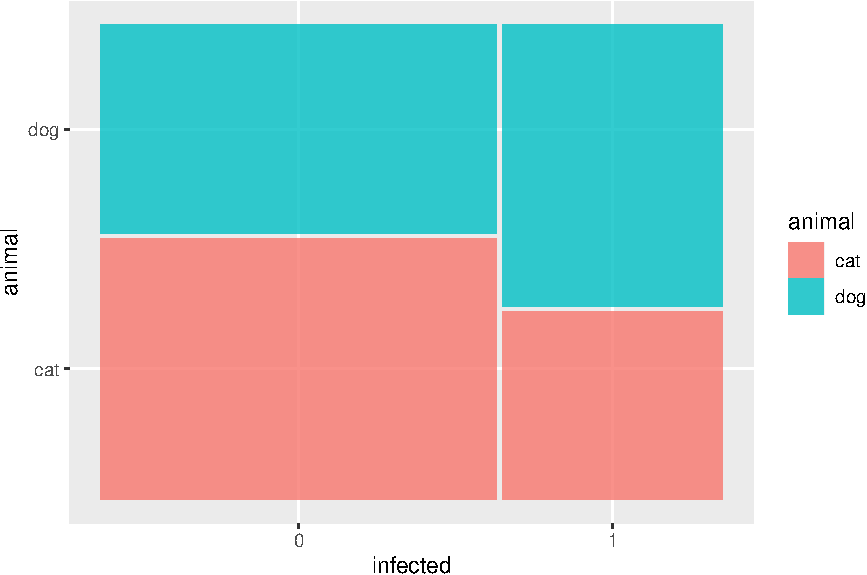
\includegraphics{./eda-ggplot_files/figure-pdf/fig-mosaic-flea-0-1.pdf}

}

\caption{\label{fig-mosaic-flea-0}Visualisierung einer 2x2 Tabelle als
Mosaic Plot. Die unterschiedlich großen Flächen geben die Verhältnisse
wieder.}

\end{figure}

Abbildung~\ref{fig-mosaic-flea-0} zeigt den Mosaic Plot für die Variable
\texttt{animal} and \texttt{infected}. Die untrschiedlich großen Flächen
bilden die Verhältnisse der 2x2 Tabelle ab. So sehen wir, dass es mehr
uninfizierte Tiere als infizierte Tiere gibt. Am meisten gibt es
uninfizierte Katzen. Am wenigstens treten infizierte Katzen auf.

\hypertarget{uxfcberschriften-achsen-und-legenden}{%
\section{Überschriften, Achsen und
Legenden}\label{uxfcberschriften-achsen-und-legenden}}

Wenn du mehr machen willst, also die Überschriften anpassen oder aber
die Achsenbeschriftung ändern, dann gibt es hier global Hilfe im
\href{https://ggplot2.tidyverse.org/reference/index.html}{ggplot
Manual}. Die Webseite
\href{https://ggplot2.tidyverse.org/reference/index.html}{R Cookbook}
hat auch spezielle Hilfe für ggplot().

\begin{itemize}
\tightlist
\item
  \href{http://www.cookbook-r.com/Graphs/Titles_(ggplot2)/}{Überschriften
  von Abbildungen}
\item
  \href{http://www.cookbook-r.com/Graphs/Axes_(ggplot2)/}{Achsenbeschriftung}
\item
  \href{http://www.cookbook-r.com/Graphs/Legends_(ggplot2)/}{Legende}
\item
  \href{http://www.cookbook-r.com/Graphs/Colors_(ggplot2)/}{Farben}
\end{itemize}

{\marginnote{\begin{footnotesize}Im Kapitel~\ref{sec-r-tutorium} findest
du Informationen zum R Tutorium, wann und wo es
stattfindet.\end{footnotesize}}}

In Abbildung~\ref{fig-labels-0} siehst du eine Abbildung mit Titel und
veränderten Beschriftungen. Die Möglichkeiten sind nahezu unbegrenzt und
sprengen auch hier den Rahmen. Im Zweifel im R Tutorium vorbeischauen
oder aber in der Vorlesung fragen.

\begin{Shaded}
\begin{Highlighting}[]
\FunctionTok{ggplot}\NormalTok{(}\AttributeTok{data =}\NormalTok{ flea\_dog\_cat\_tbl, }\FunctionTok{aes}\NormalTok{(}\AttributeTok{x =}\NormalTok{ animal, }\AttributeTok{y =}\NormalTok{ jump\_length,}
                                    \AttributeTok{fill =}\NormalTok{ animal)) }\SpecialCharTok{+}
  \FunctionTok{geom\_boxplot}\NormalTok{() }\SpecialCharTok{+}
  \FunctionTok{labs}\NormalTok{(}\AttributeTok{title =} \StringTok{"Frischgewicht in Abhängigkeit von der Behandlung"}\NormalTok{,}
       \AttributeTok{x =} \StringTok{"Behandlung"}\NormalTok{, }\AttributeTok{y =} \StringTok{"Frischgewicht in kg/ha"}\NormalTok{) }\SpecialCharTok{+}
  \FunctionTok{scale\_x\_discrete}\NormalTok{(}\AttributeTok{labels =} \FunctionTok{c}\NormalTok{(}\StringTok{"Katze"}\NormalTok{, }\StringTok{"Hund"}\NormalTok{)) }\SpecialCharTok{+}
  \FunctionTok{scale\_fill\_discrete}\NormalTok{(}\AttributeTok{name =} \StringTok{"Behandlung"}\NormalTok{, }\AttributeTok{labels =} \FunctionTok{c}\NormalTok{(}\StringTok{"Katze"}\NormalTok{, }\StringTok{"Hund"}\NormalTok{)) }\SpecialCharTok{+}
  \FunctionTok{theme\_bw}\NormalTok{() }
\end{Highlighting}
\end{Shaded}

\begin{figure}[H]

{\centering 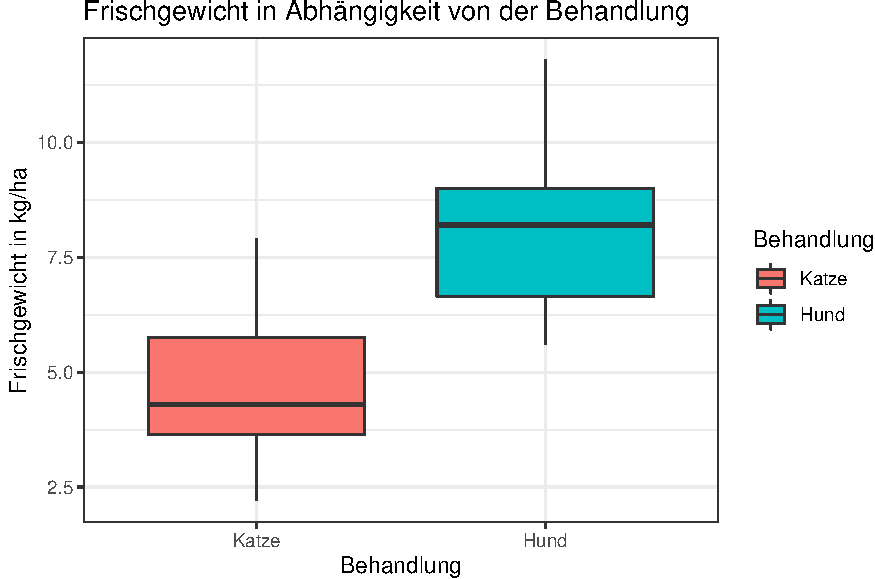
\includegraphics{./eda-ggplot_files/figure-pdf/fig-labels-0-1.pdf}

}

\caption{\label{fig-labels-0}Beispielhafte Abbildung mit Titel und
geänderter Achsenbeschrittung}

\end{figure}

\hypertarget{die-okabe-ito-farbpalette}{%
\section{Die Okabe-Ito Farbpalette}\label{die-okabe-ito-farbpalette}}

\marginnote{\begin{footnotesize}

Mehr zum R Paket \texttt{see} auf der
\href{https://easystats.github.io/see/index.html}{Hilfeseite des
Paketes}

\end{footnotesize}}

Neben den klassischen Farben im R Paket \texttt{ggplot}gibt es noch
weit, weit mehr Farbpaletten. Wir nutzen in der Folge immer wieder die
Okabe-Ito Farbpalette aus dem R Paket \texttt{see}. Die Okabe-Ito
Farbpalette ist speziell so gebaut, dass die Farben sich gut für
farbenblinde Personen unterscheiden. Der Kontrast zwischen den Farben
ist sehr gut. Wenn du eine andere Farbpalette nutzen willst, findest du
hier noch andere
\href{https://easystats.github.io/see/articles/seecolorscales.html}{Color
Scales}.

\begin{Shaded}
\begin{Highlighting}[]
\FunctionTok{ggplot}\NormalTok{(}\AttributeTok{data =}\NormalTok{ flea\_dog\_cat\_tbl, }
       \FunctionTok{aes}\NormalTok{(}\AttributeTok{x =}\NormalTok{ animal, }\AttributeTok{y =}\NormalTok{ jump\_length,}
           \AttributeTok{fill =}\NormalTok{ animal)) }\SpecialCharTok{+}
  \FunctionTok{geom\_boxplot}\NormalTok{() }\SpecialCharTok{+}
  \FunctionTok{scale\_fill\_okabeito}\NormalTok{() }\SpecialCharTok{+}
  \FunctionTok{theme\_bw}\NormalTok{()}
\end{Highlighting}
\end{Shaded}

\begin{figure}[H]

{\centering 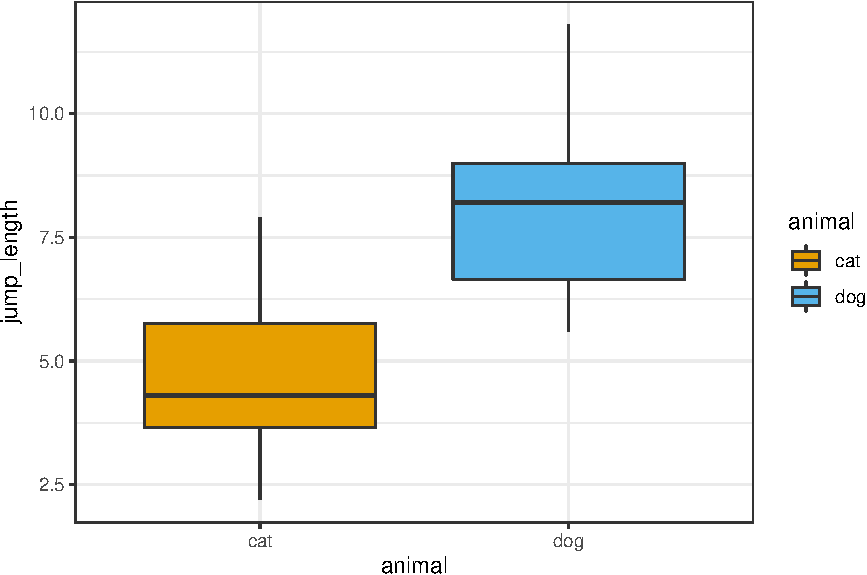
\includegraphics{./eda-ggplot_files/figure-pdf/fig-labels-see-0-1.pdf}

}

\caption{\label{fig-labels-see-0}Beispielhafte Abbildung der Okabe-Ito
Farbpalette für Boxplots.}

\end{figure}

\begin{Shaded}
\begin{Highlighting}[]
\FunctionTok{ggplot}\NormalTok{(}\AttributeTok{data =}\NormalTok{ flea\_dog\_cat\_tbl, }
       \FunctionTok{aes}\NormalTok{(}\AttributeTok{x =}\NormalTok{ animal, }\AttributeTok{y =}\NormalTok{ jump\_length,}
           \AttributeTok{color =}\NormalTok{ animal)) }\SpecialCharTok{+}
  \FunctionTok{geom\_point}\NormalTok{() }\SpecialCharTok{+}
  \FunctionTok{scale\_color\_okabeito}\NormalTok{() }\SpecialCharTok{+}
  \FunctionTok{theme\_bw}\NormalTok{()}
\end{Highlighting}
\end{Shaded}

\begin{figure}[H]

{\centering 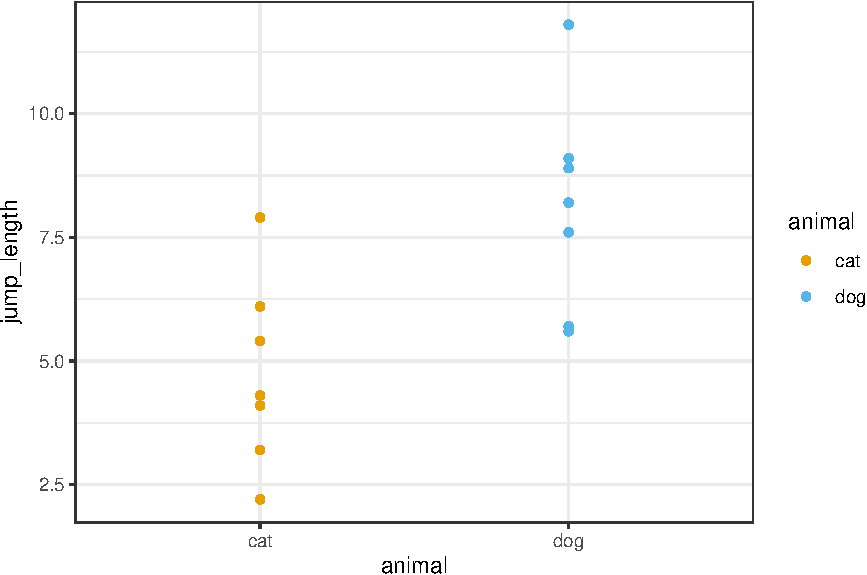
\includegraphics{./eda-ggplot_files/figure-pdf/fig-labels-see-1-1.pdf}

}

\caption{\label{fig-labels-see-1}Beispielhafte Abbildung der Okabe-Ito
Farbpalette für Punkte.}

\end{figure}

\hypertarget{abbildungen-nebeneinander}{%
\section{Abbildungen nebeneinander}\label{abbildungen-nebeneinander}}

Das
\href{https://patchwork.data-imaginist.com/articles/patchwork.html}{R
Paket patchwork} erlaubt es mehrere \texttt{ggplot} Abbildungen
nebeneinander oder in einem beliebigen Layout miteinander zu verbinden.
Das tolle ist, dass die Idee sehr intutiv ist. Wir nutzen wieder das
\texttt{+} um verschiedene Plots miteinander zu verbinden.

Im Folgenden erschaffen wir uns zwei \texttt{ggplots} und speichern die
Plots in den Objekten \texttt{p1} und \texttt{p2}. Das ist wie wir es
bisher kennen, nur das jetzt keine Abbildung erscheint sondern beide
Plots in zwei Objekten gespeichert sind.

\begin{Shaded}
\begin{Highlighting}[]
\NormalTok{p1 }\OtherTok{\textless{}{-}} \FunctionTok{ggplot}\NormalTok{(}\AttributeTok{data =}\NormalTok{ flea\_dog\_cat\_tbl, }
             \FunctionTok{aes}\NormalTok{(}\AttributeTok{x =}\NormalTok{ flea\_count, }\AttributeTok{y =}\NormalTok{ jump\_length,}
                 \AttributeTok{color =}\NormalTok{ animal)) }\SpecialCharTok{+}
  \FunctionTok{geom\_point}\NormalTok{() }\SpecialCharTok{+}
  \FunctionTok{scale\_color\_okabeito}\NormalTok{() }\SpecialCharTok{+}
  \FunctionTok{theme\_bw}\NormalTok{()}

\NormalTok{p2 }\OtherTok{\textless{}{-}} \FunctionTok{ggplot}\NormalTok{(}\AttributeTok{data =}\NormalTok{ flea\_dog\_cat\_tbl, }
                \FunctionTok{aes}\NormalTok{(}\AttributeTok{x =}\NormalTok{ animal, }\AttributeTok{y =}\NormalTok{ jump\_length,}
                    \AttributeTok{color =}\NormalTok{ animal)) }\SpecialCharTok{+}
  \FunctionTok{geom\_point}\NormalTok{() }\SpecialCharTok{+}
  \FunctionTok{scale\_color\_okabeito}\NormalTok{() }\SpecialCharTok{+}
  \FunctionTok{theme\_bw}\NormalTok{()}
\end{Highlighting}
\end{Shaded}

Wie können wir nun die beiden Abbildungen nebeneinander zeichnen? Wir
nutzen einfach das \texttt{+} Symbol.

\begin{Shaded}
\begin{Highlighting}[]
\NormalTok{p1 }\SpecialCharTok{+}\NormalTok{ p2}
\end{Highlighting}
\end{Shaded}

\begin{figure}[H]

{\centering 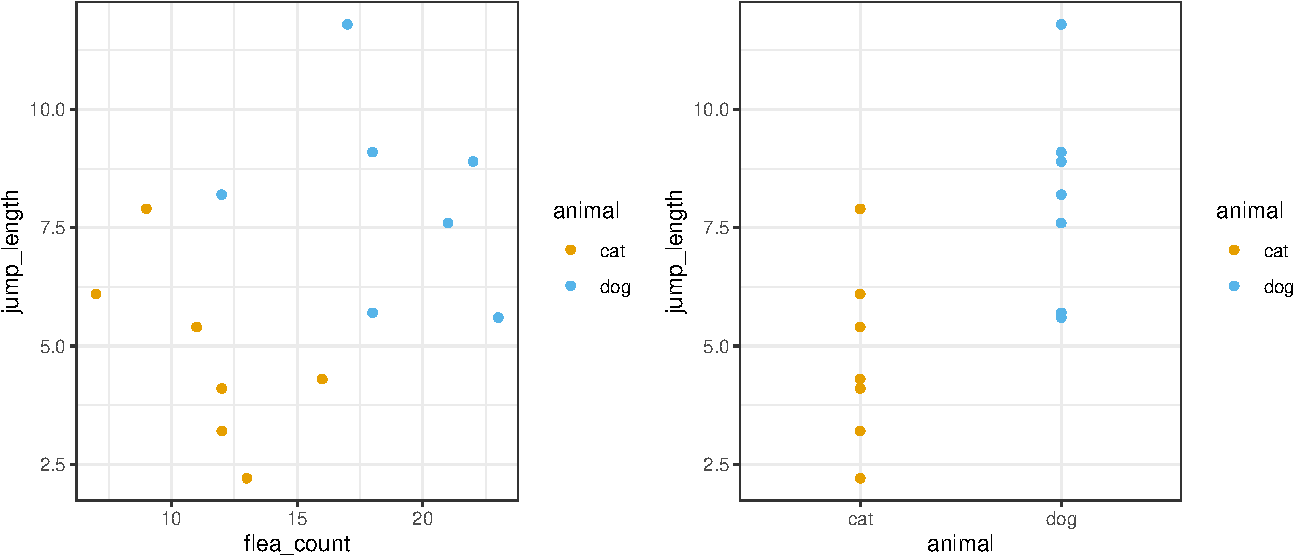
\includegraphics{./eda-ggplot_files/figure-pdf/fig-labels-patchwork-1-1.pdf}

}

\caption{\label{fig-labels-patchwork-1}Beispielhafte Abbildung der
zweier Plots nebeneinander.}

\end{figure}

Auf der Seite des
\href{https://patchwork.data-imaginist.com/articles/patchwork.html}{R
Paket patchwork} findest du viel mehr Möglichkeiten das Layout
anzupassen und auch die einzelnen
\href{https://patchwork.data-imaginist.com/articles/guides/annotation.html}{Subplots
zu beschriften}.

\hypertarget{sec-eda-transform}{%
\chapter{Transformieren von Daten}\label{sec-eda-transform}}

\emph{Version vom September 14, 2022 um 08:47:40}

\marginnote{\begin{footnotesize}

Ich verweise hier auch nochmal auf das tolle Tutorial von Matus Seci auf
dem
\href{https://ourcodingclub.github.io/tutorials/data-scaling/}{Coding
Club}

\end{footnotesize}}

Warum müssen wir Daten transformieren? Meistens hat dies zwei
Hauptgründe.

\begin{enumerate}
\def\labelenumi{\arabic{enumi})}
\tightlist
\item
  Wir wollen eine ANOVA oder eine Gaussian lineare Regression rechen und
  benötigen ein normalverteiltes Outcome \(y\)
\item
  Wir wollen einen Algorithmus zur Prädiktion (deu. \emph{Vorhersage})
  nutzen und haben sehr viele Einflussvariablen \(x\) in sehr
  unterschiedlichen Einheiten.
\end{enumerate}

Im ersten Fall wollen wir meist unsere Daten \(log\)-Transformieren um
aus einem \emph{nicht}-normalverteilten Outcome \(y\) ein
\(log\)-normalverteiltes \(y\) zu erschaffen. Im zweiten Fall wollen wir
unsere Daten Standardisieren oder Normalisieren. Wir brauchen
normalisierte Daten später beim Klassifizieren im Rahmen von
maschinellen Lernverfahren.

Wir wollen uns nun die Verfahren zur Transformation von Daten in den
folgenden Abschnitten einmal alle anschauen.

\hypertarget{genutzte-r-pakete-fuxfcr-das-kapitel-3}{%
\section{Genutzte R Pakete für das
Kapitel}\label{genutzte-r-pakete-fuxfcr-das-kapitel-3}}

Wir wollen folgende R Pakete in diesem Kapitel nutzen.

\begin{Shaded}
\begin{Highlighting}[]
\NormalTok{pacman}\SpecialCharTok{::}\FunctionTok{p\_load}\NormalTok{(tidyverse, magrittr, conflicted)}
\FunctionTok{conflict\_prefer}\NormalTok{(}\StringTok{"select"}\NormalTok{, }\StringTok{"dplyr"}\NormalTok{)}
\FunctionTok{conflict\_prefer}\NormalTok{(}\StringTok{"filter"}\NormalTok{, }\StringTok{"dplyr"}\NormalTok{)}
\end{Highlighting}
\end{Shaded}

Am Ende des Kapitels findest du nochmal den gesamten R Code in einem
Rutsch zum selber durchführen oder aber kopieren.

\hypertarget{daten}{%
\section{Daten}\label{daten}}

Wir wollen uns in diesem Kapitel mit der normalverteilten Variable
\texttt{jump\_length} gemessen in {[}cm{]} und der
nicht-normalverteilten Variable \texttt{hatch\_time} gemessen in {[}h{]}
aus dem Datensatz \texttt{flea\_dog\_cat\_length\_weight.csv"}
beschäftigen. Wir wählen über die Funktion \texttt{select()} nur die
beiden Spalten aus dem Datensatz, die wir benötigen.

\begin{Shaded}
\begin{Highlighting}[]
\NormalTok{data\_tbl }\OtherTok{\textless{}{-}} \FunctionTok{read\_csv2}\NormalTok{(}\StringTok{"data/flea\_dog\_cat\_length\_weight.csv"}\NormalTok{) }\SpecialCharTok{\%\textgreater{}\%}
  \FunctionTok{select}\NormalTok{(jump\_length, hatch\_time)}
\end{Highlighting}
\end{Shaded}

In der Tabelle~\ref{tbl-trans-1} ist der Datensatz \texttt{data\_tbl}
nochmal dargestellt. Wir zeigen hier nur die ersten sieben zeilen des
Datensatzes.

\hypertarget{tbl-trans-1}{}
\begin{longtable}[]{@{}cc@{}}
\caption{\label{tbl-trans-1}Selektierter Datensatz mit einer
normalverteilten Variable \texttt{jump\_length} und der
nicht-normalverteilten Variable \texttt{hatch\_time}. Wir betrachten die
ersten sieben Zeilen des Datensatzes.}\tabularnewline
\toprule()
jump\_length & hatch\_time \\
\midrule()
\endfirsthead
\toprule()
jump\_length & hatch\_time \\
\midrule()
\endhead
15.79 & 483.60 \\
18.33 & 82.56 \\
17.58 & 296.73 \\
14.09 & 140.90 \\
18.22 & 162.20 \\
13.49 & 167.47 \\
16.28 & 291.20 \\
\bottomrule()
\end{longtable}

Im Folgenden nutzen wir oft die Funktion \texttt{mutate()}. Schau dir im
Zweifel nochmal im Kapitel zu Programmierung die Funktion
\texttt{mutate()} an.

\hypertarget{log-transformation}{%
\section{\texorpdfstring{\(log\)-Transformation}{log-Transformation}}\label{log-transformation}}

Wir nutzen die \(log\)-Transformation, wenn wir aus einem
nicht-normalverteiltem Outcome \(y\) ein approxomativ normalverteiltes
Outcome \(y\) machen wollen. Dabei ist wichtig, dass wir natürlich auch
die Einheit mit \(log\)-transformieren.

Im Folgenden sehen wir die \(log\)-Transformation der Variable
\texttt{hatch\_time} mit der Funktion \texttt{log()}. Wir erschaffen
eine neue Spalte im \texttt{tibble} damit wir die beiden Variable vor
und nach der \(log\)-Transformation miteinander vergleichen können.

\begin{Shaded}
\begin{Highlighting}[]
\NormalTok{log\_tbl }\OtherTok{\textless{}{-}}\NormalTok{ data\_tbl }\SpecialCharTok{\%\textgreater{}\%} 
  \FunctionTok{mutate}\NormalTok{(}\AttributeTok{log\_hatch\_time =} \FunctionTok{log}\NormalTok{(hatch\_time))}
\end{Highlighting}
\end{Shaded}

Wir können dann über ein Histogramm die beiden Verteilungen anschauen.
In Abbildung~\ref{fig-log-scale-1-1} sehen wir die nicht transformierte,
rohe Daten. Es gibt einen klaren Peak Schlüpfzeiten am Anfang. Dann
läuft die Verteilung langsam aus. Wir können nicht annehmen, dass die
Schlüpfzeiten normalverteilt sind. Abbildung~\ref{fig-log-scale-1-2}
zeigt die \(log\)-transmutierten Daten. In diesem Fall sehen wir
normalverteilte Daten. Wir haben also ein \(log\) normalverteiltes
Outcome \(y\) mit dem wir jetzt weiterechnen können.

\begin{figure*}

\begin{minipage}[t]{0.50\linewidth}

{\centering 

\raisebox{-\height}{

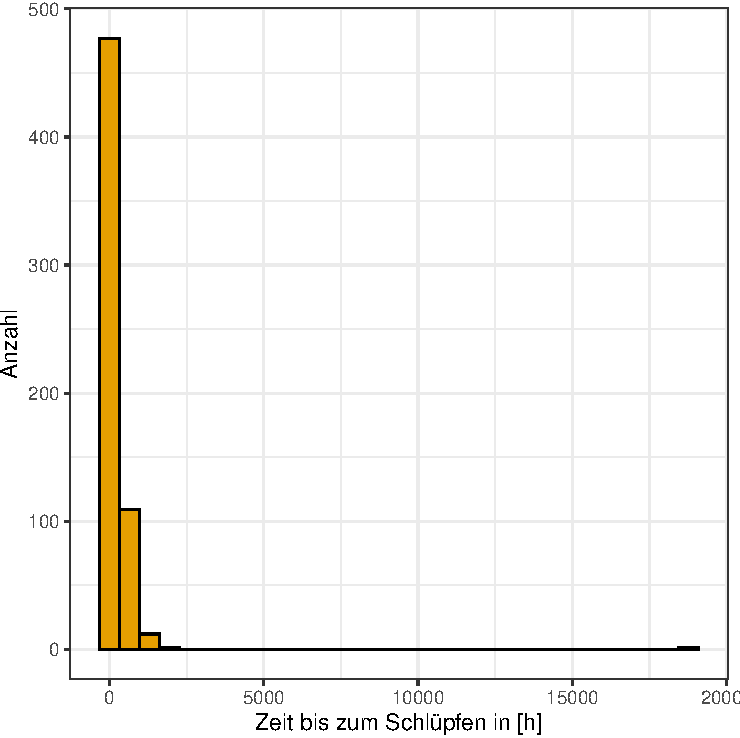
\includegraphics{./eda-transform_files/figure-pdf/fig-log-scale-1-1.pdf}

}

}

\subcaption{\label{fig-log-scale-1-1}Nicht transformierte, rohe Daten}
\end{minipage}%
%
\begin{minipage}[t]{0.50\linewidth}

{\centering 

\raisebox{-\height}{

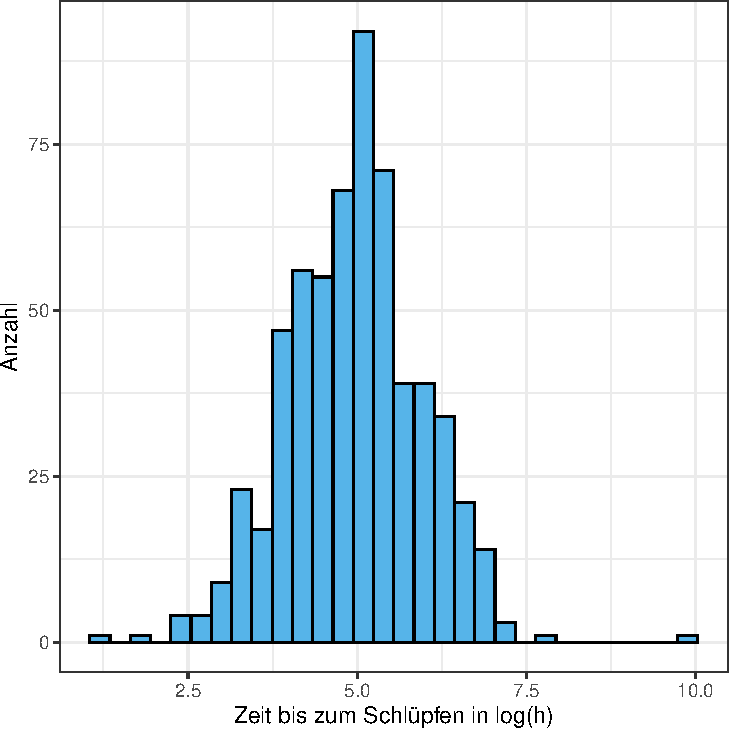
\includegraphics{./eda-transform_files/figure-pdf/fig-log-scale-1-2.pdf}

}

}

\subcaption{\label{fig-log-scale-1-2}\(log\)-transformierte Daten.}
\end{minipage}%

\caption{\label{fig-log-scale-1}Histogramm der nicht transfomierten und
transformierten Daten.}

\end{figure*}

\hypertarget{quadratwurzel-transformationen}{%
\section{Quadratwurzel-Transformationen}\label{quadratwurzel-transformationen}}

Die Quadratwurzel-Transformationen ist eine etwas seltenere
Transformation. Meist wird die Quadratwurzel-Transformationen als die
schwächere \(log\)-Transformation bezeichnet. Wir sehen in
Abbildung~\ref{fig-log-scale-2-2} den Grund dafür. Aber zuerst müssen
wir aber über die Funktion \texttt{sqrt()} unsere Daten transformieren.

\begin{Shaded}
\begin{Highlighting}[]
\NormalTok{sqrt\_tbl }\OtherTok{\textless{}{-}}\NormalTok{ data\_tbl }\SpecialCharTok{\%\textgreater{}\%} 
  \FunctionTok{mutate}\NormalTok{(}\AttributeTok{sqrt\_hatch\_time =} \FunctionTok{sqrt}\NormalTok{(hatch\_time))}
\end{Highlighting}
\end{Shaded}

In Abbildung~\ref{fig-log-scale-2-1} sehen wir die nicht transformierte,
rohe Daten. Es gibt einen klaren Peak Schlüpfzeiten am Anfang. Dann
läuft die Verteilung langsam nach rechts aus. Wir können nicht annehmen,
dass die Schlüpfzeiten normalverteilt sind.
Abbildung~\ref{fig-log-scale-2-2} zeigt die Wurzel-transmutierten Daten.
Unser Ziel besser normalverteilte Daten vorliegen zu haben, haben wir
aber mit der Quadratwurzel-Transformationen nicht erreicht. Die Daten
sind immer noch rechtsschief. Wir würden also die \(log\)-Transformation
bevorzugen.

\begin{figure*}

\begin{minipage}[t]{0.50\linewidth}

{\centering 

\raisebox{-\height}{

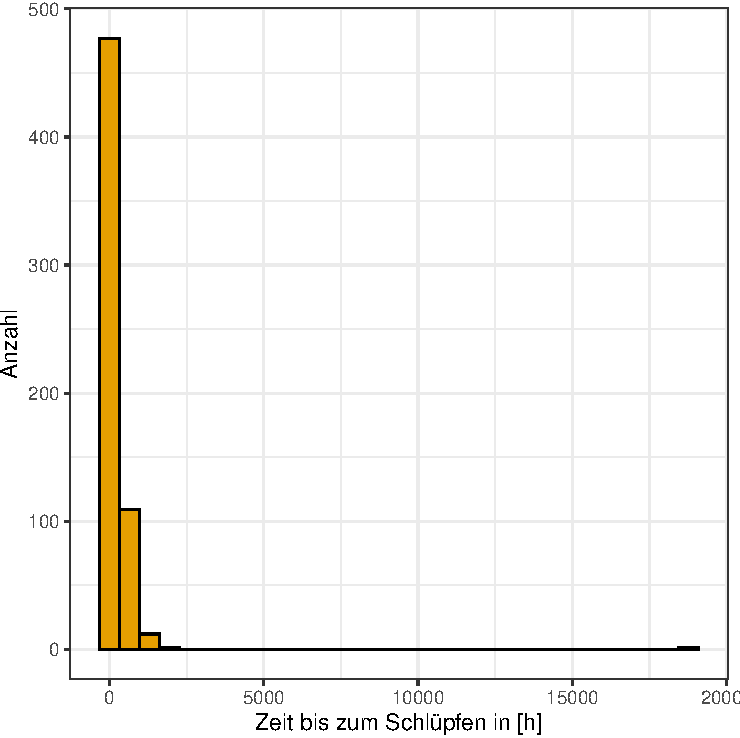
\includegraphics{./eda-transform_files/figure-pdf/fig-log-scale-2-1.pdf}

}

}

\subcaption{\label{fig-log-scale-2-1}Nicht transformierte, rohe Daten}
\end{minipage}%
%
\begin{minipage}[t]{0.50\linewidth}

{\centering 

\raisebox{-\height}{

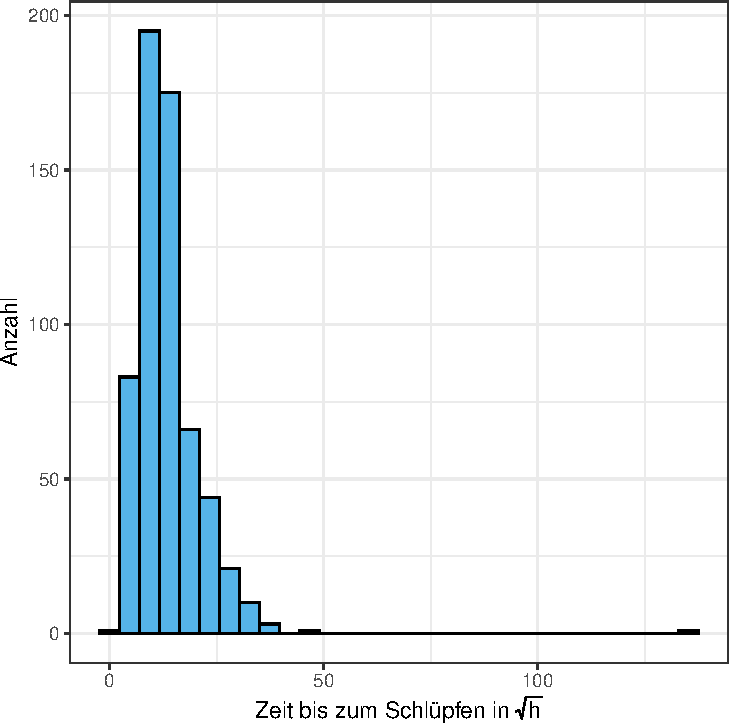
\includegraphics{./eda-transform_files/figure-pdf/fig-log-scale-2-2.pdf}

}

}

\subcaption{\label{fig-log-scale-2-2}Wurzel-transformierte Daten.}
\end{minipage}%

\caption{\label{fig-log-scale-2}Histogramm der nicht transfomierten und
transformierten Daten.}

\end{figure*}

\hypertarget{standardisierung}{%
\section{Standardisierung}\label{standardisierung}}

Die Standardisierung wird auch \(z\)-Transformation genannt. In dem Fall
der Standardisierung schieben wir die Daten auf den Ursprung, in dem wir
von jedem Datenpunkt \(y_i\) den Mittelwert \(\bar{y}\) abziehen. Dann
setzen wir noch die Standardabweichung auf Eins in dem wir durch die
Standardabweichung \(y_s\) teilen. Unser standardisiertes \(y\) ist nun
standard normalverteilt mit \(\mathcal{N(0,1)}\). Wir nutzen für die
Standardisiwerung folgende Formel.

\[
y_z = \cfrac{y_i - \bar{y}}{s_y} 
\] In R können wir für die Standardisierung die Funktion
\texttt{scale()} verwenden. Wir müssen auch nichts weiter in den
Optionen von \texttt{scale()} angeben. Die Standardwerte der Funktion
sind so eingestellt, dass eine Stanardnormalverteilung berechnet wird.

\begin{Shaded}
\begin{Highlighting}[]
\NormalTok{scale\_tbl }\OtherTok{\textless{}{-}}\NormalTok{ data\_tbl }\SpecialCharTok{\%\textgreater{}\%} 
  \FunctionTok{mutate}\NormalTok{(}\AttributeTok{scale\_jump\_length =} \FunctionTok{scale}\NormalTok{(jump\_length))}
\end{Highlighting}
\end{Shaded}

In Abbildung~\ref{fig-log-scale-3-1} sehen wir nochmal die nicht
transformierten, rohen Daten. Wir haben in diesem Beispiel die
normalvertielte Variable \texttt{jump\_length} gewählt. Der Mittelwert
von \texttt{jump\_length} ist 20.51 und die Standardabweichung ist 3.77.
Ziehen wir nun von jedem Wert von \texttt{jump\_length} den Mittelwert
mit 19.3 ab, so haben wir einen neuen Schwerpunkt bei Null. Teilen wir
dann jede Zahl durch 3.36 so haben wir eine reduzierte Spannweite der
Verteilung. Es ergibt sich die Abbildung~\ref{fig-log-scale-3-2} als
Standardnormalverteilung. Die Zahlen der auf der x-Achse haben jetzt
aber keine Bedeutung mehr. Wie können die Sprungweite auf der
\(z\)-Skala nicht mehr biologisch interpretieren.

\begin{figure*}

\begin{minipage}[t]{0.50\linewidth}

{\centering 

\raisebox{-\height}{

\includegraphics{./eda-transform_files/figure-pdf/fig-log-scale-3-1.pdf}

}

}

\subcaption{\label{fig-log-scale-3-1}Nicht transformierte, rohe Daten}
\end{minipage}%
%
\begin{minipage}[t]{0.50\linewidth}

{\centering 

\raisebox{-\height}{

\includegraphics{./eda-transform_files/figure-pdf/fig-log-scale-3-2.pdf}

}

}

\subcaption{\label{fig-log-scale-3-2}\(z\)-transformierte Daten.}
\end{minipage}%

\caption{\label{fig-log-scale-3}Histogramm der nicht transfomierten und
transformierten Daten.}

\end{figure*}

\hypertarget{normalisierung}{%
\section{Normalisierung}\label{normalisierung}}

Abschließend wollen wir uns nochmal die Normalisierung anschauen. In
diesem Fall wollen wir die Daten so transformieren, dass die Daten nur
noch in der Spannweite 0 bis 1 vorkommen. Egal wie die Einheiten vorher
waren, alle Variablen haben jetzt nur noch eine Ausprägung von 0 bis 1.
Das ist besonders wichtig wenn wir viele Variablen haben und anhand der
Variablen eine Vorhersage machen wollen. Uns interessieren die Werte in
den Variablen an sich nicht, sondern wir wollen ein Outcome vorhersagen.
Wir brauchen die Normalisierung später für das maschinelle Lernen und
die Klassifikation. Die Formel für die Normalisierung lautet wie folgt.

\[
y_n = \cfrac{y_i - \min(y)}{\max(y) - \min(y)} 
\]

In R gibt es die Normalisierungsfunktion nicht direkt. Wir könnten hier
ein extra Paket laden, aber bei so einer simplen Formel können wir auch
gleich die Berechnung in der Funktion \texttt{mutate()} machen. Wir
müssen nur etwas mit den Klammern aufpassen.

\begin{figure*}

\begin{Shaded}
\begin{Highlighting}[]
\NormalTok{norm\_tbl }\OtherTok{\textless{}{-}}\NormalTok{ data\_tbl }\SpecialCharTok{\%\textgreater{}\%} 
  \FunctionTok{mutate}\NormalTok{(}\AttributeTok{norm\_jump\_length =}\NormalTok{ (jump\_length }\SpecialCharTok{{-}} \FunctionTok{min}\NormalTok{(jump\_length))}\SpecialCharTok{/}\NormalTok{(}\FunctionTok{max}\NormalTok{(jump\_length) }\SpecialCharTok{{-}} \FunctionTok{min}\NormalTok{(jump\_length)))}
\end{Highlighting}
\end{Shaded}

\end{figure*}

In Abbildung~\ref{fig-log-scale-4-1} sehen wir nochmal die nicht
transformierten, rohen Daten. In Abbildung~\ref{fig-log-scale-4-2} sehen
wir die normalisierten Daten. Hier fällt dann auf, dass die
normalisierten Sprungweiten nur noch Werte zwischen Null und Eins
annehmen. Die Zahlen der auf der x-Achse haben jetzt aber keine
Bedeutung mehr. Wie können die normalisierten Sprungweiten nicht mehr
biologisch interpretieren.

\begin{figure*}

\begin{minipage}[t]{0.50\linewidth}

{\centering 

\raisebox{-\height}{

\includegraphics{./eda-transform_files/figure-pdf/fig-log-scale-4-1.pdf}

}

}

\subcaption{\label{fig-log-scale-4-1}Nicht transformierte, rohe Daten}
\end{minipage}%
%
\begin{minipage}[t]{0.50\linewidth}

{\centering 

\raisebox{-\height}{

\includegraphics{./eda-transform_files/figure-pdf/fig-log-scale-4-2.pdf}

}

}

\subcaption{\label{fig-log-scale-4-2}Normalisierte Daten}
\end{minipage}%

\caption{\label{fig-log-scale-4}Histogramm der nicht transfomierten und
transformierten Daten.}

\end{figure*}

\hypertarget{verteilung-von-daten}{%
\chapter{Verteilung von Daten}\label{verteilung-von-daten}}

\emph{Version vom September 14, 2022 um 08:48:02}

\marginnote{\begin{footnotesize}

Wir besuchen gerne die R Shiny App
\href{https://ben18785.shinyapps.io/distribution-zoo/}{The distribution
zoo} um mehr über die verschiedenen Verteilungen und deren Parameter zu
erfahren.

\end{footnotesize}}

In diesem Kapitel wollen wir uns mit Verteilungen beschäftigen. Dormann
(2013) liefert eine weitreichende Übersicht über verschiedene
Verteilungen. Wir wollen uns in diesem Kapitel mit folgenden
Verteilungen beginnen.

\begin{itemize}
\tightlist
\item
  der \textbf{Normalverteilung}, die Glockenkurve oder auch
  \textbf{Gaussian} im englischen Sprachgebrauch genannt, die
  kontinuierliche Zahlen repräsentiert
\item
  der \textbf{Poissonverteilung}, die diskrete Zähldaten repräsentiert.
\end{itemize}

Wir wollen uns jetzt die verschiedenen Verteilungen einmal in der
Anwendung anschauen. Dabei lassen wir viel Mathematik recht und links
liegen. Du kannst bei Dormann (2013) mehr zu dem Thema statistische
Verteilungen anlesen.

In diesem Kapitel geht es erstmal um das Grundverständnis, das Daten
einer Verteilung folgen. Oder noch konkreter, dass unser Outcome \(y\)
einer Verteilung folgt. Wir müssen später unseren Alogrithmen sagen,
welcher Verteilung \(y\) entspringt, sonst können wir keine
\emph{korrekte} Analyse unser Daten rechnen.

\begin{marginfigure}

{\centering \includegraphics[width=0.5\textwidth,height=\textheight]{./images/angel_01.png}

}

\end{marginfigure}

Wir halten den mathematischen Teil zu den Verteilungen sehr kurz oder
überspringen den Teil ganz. Wir brauchen die Idee der Verteilungen, weil
wir später den Methoden sagen müssen wie unser Outcome \(y\) verteilt
ist. Nur dann können wir die Daten richtig auswerten.

\hypertarget{genutzte-r-pakete-fuxfcr-das-kapitel-4}{%
\section{Genutzte R Pakete für das
Kapitel}\label{genutzte-r-pakete-fuxfcr-das-kapitel-4}}

Wir wollen folgende R Pakete in diesem Kapitel nutzen.

\begin{Shaded}
\begin{Highlighting}[]
\NormalTok{pacman}\SpecialCharTok{::}\FunctionTok{p\_load}\NormalTok{(tidyverse, magrittr, see, readxl)}
\end{Highlighting}
\end{Shaded}

Am Ende des Kapitels findest du nochmal den gesamten R Code in einem
Rutsch zum selber durchführen oder aber kopieren.

\hypertarget{daten-fuxfcr-verteilungen}{%
\section{Daten für Verteilungen}\label{daten-fuxfcr-verteilungen}}

Damit wir uns auch eine Verteilung anschauen können bruachen wir
\emph{viele} Beobachtungen. Wir haben das ja schon bei den Histogrammen
gesehen, wenn wir ein aussagekräftiges Histogramm erstellen wollen, dann
brauchen wir viele Beobachtungen. Daher nehmen wir für dieses Kapitel
einmal den Gummibärchendatensatz und schauen uns dort die Variablen
\texttt{gender}, \texttt{height}, \texttt{count\_bears} und
\texttt{count\_color} einmal genauer an. Wie immer nutzen wir die
Funktion \texttt{select()} um die Spalten zu selektieren. Wir müssen
jetzt nochmal alle fehlenden Werte mit der Funktion \texttt{na.omit()}
entfernen, dass macht uns die Sache etwas leichter. Abschließend
verwandeln wir das Geschlecht \texttt{gender} noch in einen Faktor.

\begin{Shaded}
\begin{Highlighting}[]
\NormalTok{gummi\_tbl }\OtherTok{\textless{}{-}} \FunctionTok{read\_excel}\NormalTok{(}\StringTok{"data/gummibears.xlsx"}\NormalTok{)  }\SpecialCharTok{\%\textgreater{}\%}
  \FunctionTok{select}\NormalTok{(gender, height, count\_bears, count\_color) }\SpecialCharTok{\%\textgreater{}\%} 
  \FunctionTok{na.omit}\NormalTok{() }\SpecialCharTok{\%\textgreater{}\%} 
  \FunctionTok{mutate}\NormalTok{(}\AttributeTok{gender =} \FunctionTok{as\_factor}\NormalTok{(gender))}
\end{Highlighting}
\end{Shaded}

Wir erhalten das Objekt \texttt{gummi\_tbl} mit dem Datensatz in
Tabelle~\ref{tbl-data-dist-gummi} nochmal dargestellt.

\hypertarget{tbl-data-dist-gummi}{}
\begin{longtable}[]{@{}cccc@{}}
\caption{\label{tbl-data-dist-gummi}Auszug aus den selektierten Daten zu
den Gummibärchendaten.}\tabularnewline
\toprule()
gender & height & count\_bears & count\_color \\
\midrule()
\endfirsthead
\toprule()
gender & height & count\_bears & count\_color \\
\midrule()
\endhead
m & 193 & 9 & 3 \\
w & 159 & 10 & 5 \\
w & 159 & 9 & 6 \\
w & 180 & 10 & 5 \\
m & 180 & 10 & 6 \\
m & 180 & 10 & 5 \\
\ldots{} & \ldots{} & \ldots{} & \ldots{} \\
w & 165 & 12 & 5 \\
w & 177 & 10 & 2 \\
w & 173 & 9 & 5 \\
w & 168 & 12 & 6 \\
m & 183 & 8 & 5 \\
w & 171 & 9 & 5 \\
\bottomrule()
\end{longtable}

Wir nutzen jetzt die Daten einmal um uns die Normalverteilung und die
Poissonverteilung am Beispiel näher anzuschauen.

\hypertarget{sec-normal}{%
\section{Die Normalverteilung}\label{sec-normal}}

{\marginnote{\begin{footnotesize}Wir sprechen in der Statistik auch von
Verteilungs\emph{familien}. Daher schreiben wir in R auch
\texttt{family\ =\ gaussian}, wenn wir sagen wollen, dass unsere Daten
einer Normalverteilung entstammen.\end{footnotesize}}}

Wenn wir von de Normalverteilung sprechen, dann schreiben wir ein
\(\mathcal{N}\) Symbol - also ein großes N mit Serifen. Die
Normalverteilung sieht aus wie eine Glocke, deshalb wird die
Normalverteilung auch Glockenkurve genannt. Im englischen Sprachgebrauch
und auch in R nutzen wir dagegen die Bezeichnung nach dem ``Endecker''
der Normalverteilung, Carl Friedrich Gauß (1777 - 1985). Wir nennen
daher die Normalverteilung auch Gaussian-Verteilung.

{\marginnote{\begin{footnotesize}\textbf{Parameter} sind Zahlen, die
eine Verteilungskurve beschreiben.\end{footnotesize}}}

Eine Normalverteilung wird ruch zwei Verteilungs\emph{parameter}
definiert. Eine Verteilung hat Parameter. Parameter sind die
Eigenschaften einer Verteilung, die notwendig sind um eine Verteilung
vollständig zu beschreiben. Im Falle der Normalverteilung brauchen wir
zum einen den Mittelwert \(\bar{y}\), der den höchsten Punkt unserer
Glockenkurve beschreibt. Zum anderen brauchen wir auch die
Standardabweichung \(s^2_y\), die die Ausbreitung oder Breite der
Glockenkurve bestimmt. Wir beschreiben eine Normalverteilung wie folgt.

\[
\mathcal{N}(\bar{y}, s^2_y)
\] Im Falle der Normalverteilung brauchen wir einen Paramter für den
höchsten Punkt der Kurve, sowie einen Parameter für die Ausbreitung,
also wie weit geht die Kurve nach links und nach rechts. Je nach
\(\bar{y}\) und \(s^2_y\) können wir verschiedenste Normalverteilungen
vorliegen haben. Eine Sammlung von Normalverteilungen nennen wir auch
Familie (eng. \emph{family}).

{\marginnote{\begin{footnotesize}Wir haben Varianzhomogenität vorliegen,
wenn \(s^2_{1} = s^2_{2} = s^2_{3}\) sind. Wir haben
Varianzheterogenität vorliegen, wenn
\(s^2_{1} \neq s^2_{2} \neq s^2_{3}\) sind.\end{footnotesize}}}

In Abbildung~\ref{fig-normal-02} sehen wir verschiedene
Normalverteilungen mit unterschiedlichen Mittelwerten. In
Abbildung~\ref{fig-normal-02-1} sehen wir eine Varianzhomogenität
vorliegen, da die Varianzen in allen drei Normalverteilungen gleich
sind. Wir können auch schreiben, dass
\(s^2_{1} = s^2_{2} = s^2_{3} = 2\). In Abbildung~\ref{fig-normal-02-2}
haben wir Varianzheterogenität vorliegen, da die Varianzen der
Normalverteilungen ungleich sind. Wir können hier dann schreiben, dass
\(s^2_{1} = 6 \neq s^2_{2} = 1 \neq s^2_{3} = 3\) sind. Häufig gehen
statistische Verfahren davon aus, dass wir Varianzhomogenität über die
Gruppen und daher auch die Normalverteilungen vorliegen haben. Konkret,
wenn wir die Sprungweiten in{[}cm{]} von Hunde- und Katzenflöhen mit
einander vergleichen wollen, dann gehen wir erstmal davon aus, dass die
Mittelwerte verschieden sind, aber die Varianzen gleich sind.

\begin{figure*}

\begin{minipage}[t]{0.50\linewidth}

{\centering 

\raisebox{-\height}{

\includegraphics{./eda-distribution_files/figure-pdf/fig-normal-02-1.pdf}

}

}

\subcaption{\label{fig-normal-02-1}Drei Normalverteilungen mit
Varianzhomogenität.}
\end{minipage}%
%
\begin{minipage}[t]{0.50\linewidth}

{\centering 

\raisebox{-\height}{

\includegraphics{./eda-distribution_files/figure-pdf/fig-normal-02-2.pdf}

}

}

\subcaption{\label{fig-normal-02-2}Drei Normalverteilungen unter
Varianzheterogenität.}
\end{minipage}%

\caption{\label{fig-normal-02}Histogramm verschiedener
Normalverteilungen mit unterschiedlichen Mittelwerten.}

\end{figure*}

{\marginnote{\begin{footnotesize}In einer Normalverteilung liegen 68\%
der Werte innerhalb \(\bar{y}\pm 1 \cdot s_y\) und 95\% der Werte
innerhalb \(\bar{y}\pm 2 \cdot s_y\)\end{footnotesize}}}

Wenn wir eine Normalverteilung vorliegen haben, dann liegen 68\% der
Werte plus/minus einer Standardabweichung vom Mittelwert. Ebenso liegen
95\% der Werte plus/minus zwei Standabweichungen vom Mittelwert. Über
99\% der Werte befinden sich innerhalb von drei Standardabweichungen vom
Mittelwert. Diese Eigenschaft einer Normalverteilung können wir später
noch nutzen um abzuschätzen, ob wir einen relevanten Gruppenunterschied
vorliegen haben oder aber ob unsere Daten \emph{unnatürlich} breit
streuen.

{\marginnote{\begin{footnotesize}Wir nutzen das Wort
\textbf{approximativ} wenn wir sagen wollen, dass ein Outcome
näherungsweise normalverteilt ist.\end{footnotesize}}}

Schauen wir uns die Normalverteilung einmal am Beispiel unserer
Gummibärchendaten und der Körpergröße der Studierenden an. Wir färben
das Histogramm nach dem Geschlecht ein. In Abbildung~\ref{fig-normal-01}
sehen wir das Ergebnis einmal als Histogramm und einmal als Densityplot
dargestellt. Wir können annehmen, dass die Größe \emph{approximativ}
normalverteilt ist.

\begin{figure*}

\begin{minipage}[t]{0.50\linewidth}

{\centering 

\raisebox{-\height}{

\includegraphics{./eda-distribution_files/figure-pdf/fig-normal-01-1.pdf}

}

}

\subcaption{\label{fig-normal-01-1}Histogramm.}
\end{minipage}%
%
\begin{minipage}[t]{0.50\linewidth}

{\centering 

\raisebox{-\height}{

\includegraphics{./eda-distribution_files/figure-pdf/fig-normal-01-2.pdf}

}

}

\subcaption{\label{fig-normal-01-2}Densityplot.}
\end{minipage}%

\caption{\label{fig-normal-01}Darstellung der Körpergröße in {[}cm{]}
für die Geschlechter getrennt.}

\end{figure*}

Wir können die Funktion \texttt{rnorm()} nutzen um uns zufällige Zahlen
aus der Normalverteilung ziehen zu lassen. Dazu müssen wir mit
\texttt{n\ =} spezifizieren wie viele Beobachtungen wir wollen und den
Mittelwert \texttt{mean\ =} und die gewünschte Standardabweichung mit
\texttt{sd\ =} angeben. Im Folgenden einmal ein Beispiel für die Nutzung
der Funktion \texttt{rnorm()} mit zehn Werten.

\begin{Shaded}
\begin{Highlighting}[]
\FunctionTok{rnorm}\NormalTok{(}\AttributeTok{n =} \DecValTok{10}\NormalTok{, }\AttributeTok{mean =} \DecValTok{5}\NormalTok{, }\AttributeTok{sd =} \DecValTok{2}\NormalTok{) }\SpecialCharTok{\%\textgreater{}\%} \FunctionTok{round}\NormalTok{(}\DecValTok{2}\NormalTok{)}
\end{Highlighting}
\end{Shaded}

\begin{verbatim}
 [1] 6.97 6.24 5.59 5.27 6.30 4.91 4.13 4.92 3.67 4.42
\end{verbatim}

Du kannst ja mal den Mittelwert und die Standardabweichung der zehn
Zahlen ausrechnen. Da wir es hier mit einer Stichprobe mit zehn
Beobachtungen zu tun haben, wird der Mittelwert \(\bar{y}\) und die
Standardabweichung \(s_y\) sich von den vorher definierten Mittelwert
\(\mu_y = 5\) und Standardabweichung \(\sigma_y = 2\) der
Grundgesamtheit unterscheiden.

Wir können auch aus unseren Gummibärchendaten für die Körpergröße in
{[}cm{]} jeweils den Mittelwert und die Standardabweichung getrennt für
die Geschlechter berechnen und dann die theoretische Normalverteilung
zeichenen. In Abbildung~\ref{fig-normal-03-2} und
Abbildung~\ref{fig-normal-03-4} sehen wir die Verteilung der
theoretischen Werte, wenn wir die Mittelwerte und die Standardabweichung
aus den Verteilungen in Abbildung~\ref{fig-normal-03-1} schätzen.

\begin{figure*}

\begin{minipage}[t]{0.50\linewidth}

{\centering 

\raisebox{-\height}{

\includegraphics{./eda-distribution_files/figure-pdf/fig-normal-03-1.pdf}

}

}

\subcaption{\label{fig-normal-03-1}Verteilung der beobachteten Werte.}
\end{minipage}%
%
\begin{minipage}[t]{0.50\linewidth}

{\centering 

\raisebox{-\height}{

\includegraphics{./eda-distribution_files/figure-pdf/fig-normal-03-2.pdf}

}

}

\subcaption{\label{fig-normal-03-2}Verteilung der theoretischen Werte.}
\end{minipage}%
\newline
\begin{minipage}[t]{0.50\linewidth}

{\centering 

\raisebox{-\height}{

\includegraphics{./eda-distribution_files/figure-pdf/fig-normal-03-3.pdf}

}

}

\subcaption{\label{fig-normal-03-3}Verteilung der beobachteten Werte.}
\end{minipage}%
%
\begin{minipage}[t]{0.50\linewidth}

{\centering 

\raisebox{-\height}{

\includegraphics{./eda-distribution_files/figure-pdf/fig-normal-03-4.pdf}

}

}

\subcaption{\label{fig-normal-03-4}Verteilung der theoretischen Werte.}
\end{minipage}%

\caption{\label{fig-normal-03}Darstellung der Körpergröße in {[}cm{]}
für die Geschlechter getrennt. Auf der linken Seite die beobachteten
Werte und auf der rechten Seite die theoretischen Werte. Einmal
dargestellt als Histogramm und einmal als Densityplot.}

\end{figure*}

\hypertarget{die-standardnormalverteilung}{%
\section{Die
Standardnormalverteilung}\label{die-standardnormalverteilung}}

Es gibt viele Normalverteilungen. Aber es gibt eine besondere
Normalverteilung, so dass diese Verteilung einen eigenen Namen hat. Wir
sprechen von der Standardnormalverteilung, wenn der Mittelwert gleich
Null ist und die Standardabweichung gleich Eins. Du siehst hier nochmal
die Standardnormalverteilung ausgeschrieben.

\[
\mathcal{N}(0, 1)
\]

Folgende Eigenschaften sind der Standardnormalverteilung gegeben. Die
Standardnormalverteilung hat eine Fläche von \(A = 1\) unter der Kurve.
Darüber hinaus liegen 95\% der Werte zwischen -2 und 2. Die einzelnen
Werte einer Standardnormalverteilung nennen wir \(z\)-Werte. Wenn wir
eine beliebige Normalverteilung in eine Standardnormalverteilung
überführen wollen so machen wir die Umwandlung mit der
\(z\)-Transformation.

\hypertarget{sec-poisson}{%
\section{Die Poissonverteilung}\label{sec-poisson}}

Eine weitere wichtige Verteilung ist die Poissonverteilung. Die
Poissonverteilung ist eine diskrete Verteilung. Daher kommen nur ganze
Zahlen vor. Damit bildet die Poissonverteilung die Zähldaten ab. Wenn
wir also etwas Zählen, dann ist diese Variable mit den gezählten
Ergebnissen poissonverteilt. Im Folgenden sehen wir die
Poissonverteilung einmal dargestellt.

\[
\mathcal{Pois}(\lambda)
\]

Im Gegensatz zur Normalverteilung hat die Poissonverteilung nur einen
Parameter. Den Lageparameter \(\lambda\) ausgedrückt durch den
griechischen Buchstaben Lambda. Eine Poissonverteilung mit
\(\mathcal{Pois}(4)\) hat den höchsten Punkt bei vier. Nun hat die
Poissonverteilung hat mehrere Besonderheiten. Da die Poissonverteilung
keinen Streuungsparameter hat, steigt mit dem \(\lambda\) auch die
Streuung. Daher haben Poissonverteilungen mit einem großen \(\lambda\)
auch eine große Streuung. ie Ausbreitung der Kurve ist eine Funktion von
\(\lambda\) und steigt mit \(\lambda\) an. Du kannst diesen Zusammenhang
in Abbildung~\ref{fig-pois-00} beobachten.

Darüber hinaus kann eine Poissonverteilung nicht negativ werden. Es kann
keine kleinere Zahl als die Null geben. Durch die diskreten Zahlen haben
wir auch immer mal Lücken zwischen den Balken der Poissonverteilung. Das
passiert besonders, wenn wir eine kleine Anzahl an Beobachtungen haben.
Abschließend konvergiert die Poissonverteilung bei großen \(\lambda\)
hin zu einer Normalverteilung.

\begin{figure}

{\centering \includegraphics{./eda-distribution_files/figure-pdf/fig-pois-00-1.pdf}

}

\caption{\label{fig-pois-00}Histogramm verschiedener
Poissonverteilungen.}

\end{figure}

Schauen wir uns nun einmal die Poissonverteilung im Beispiel an. In
Abbildung~\ref{fig-pois-01} sehen wir die Histogramme der Anzahl an
Gummibärchen in einer Tüte und die Anzahl an Farben in einer Tüte. Da
wir es hier mit Zähldaten zu tun haben, könnte es sich um eine
Poissonverteilung handeln. Wie müssen uns nun die Frage stellen, ob die
Gummibärchen in einer Tüte und die Anzahl an Farben in einer Tüte
\emph{wirklich} eine zufällige Realistierung sind. Daher eine zufällige
Stichprobe der Grundgesamtheit. Wir können diese Annahme überprüfen in
dem wir die theoretischen Werte für die beiden Poissonverteilung mit
\(\mathcal{Pois}(10)\) und \(\mathcal{Pois}(5)\) genieren.

\begin{figure*}

\begin{minipage}[t]{0.50\linewidth}

{\centering 

\raisebox{-\height}{

\includegraphics{./eda-distribution_files/figure-pdf/fig-pois-01-1.pdf}

}

}

\subcaption{\label{fig-pois-01-1}Anzahl an Bärchen}
\end{minipage}%
%
\begin{minipage}[t]{0.50\linewidth}

{\centering 

\raisebox{-\height}{

\includegraphics{./eda-distribution_files/figure-pdf/fig-pois-01-2.pdf}

}

}

\subcaption{\label{fig-pois-01-2}Anzahl an Farben}
\end{minipage}%

\caption{\label{fig-pois-01}Histogramme der Anzahl an Gummibärchen und
die Anzahl an Farben in einer Tüte. Es gibt nicht mehr als sechs
Farben.}

\end{figure*}

Wir können die Funktion \texttt{rpois()} nutzen um uns zufällige Zahlen
aus der Poissonverteilung ziehen zu lassen. Dazu müssen wir mit
\texttt{n\ =} spezifizieren wie viele Beobachtungen wir wollen und den
Mittelwert \texttt{lambda\ =} angeben. Im Folgenden einmal ein Beispiel
für die Nutzung der Funktion \texttt{rpois()} mit zehn Werten.

\begin{Shaded}
\begin{Highlighting}[]
\FunctionTok{rpois}\NormalTok{(}\AttributeTok{n =} \DecValTok{10}\NormalTok{, }\AttributeTok{lambda =} \DecValTok{5}\NormalTok{)}
\end{Highlighting}
\end{Shaded}

\begin{verbatim}
 [1] 3 5 4 5 3 3 9 3 5 5
\end{verbatim}

{\marginnote{\begin{footnotesize}Es gibt neben der Poissonverteilung
auch die negative Binomialverteilung sowie die Quasi-Poissonverteilung,
die es erlauben einen Streuungsparameter für die Poissonverteilung zu
schätzen.\end{footnotesize}}}

Wir können nun auch aus unseren Gummibärchendaten für die Anzahl an
Bärchen in einer Tüte sowie die Anzahl an Farben in einer Tüte die
theoretische Poissonverteilung berechnen. In Abbildung~\ref{fig-pois-03}
sehen wir die Verteilung der beobachteten Werte für Anzahl an Bärchen in
einer Tüte sowie die Anzahl an Farben in einer Tüte und deren
theoretischen Verteilung nach dem geschätzen \(\lambda = 10\) und
\(\lambda = 5\). Wir sehen ganz klar, dass die beide Variablen
\emph{keine} Zufallsrealisierung sind. Zum einen haben wir das auch
nicht erwartet, es gibt nicht mehr als sechs Farben und zum anderen ist
zu vermuten, dass Haribo technisch in den Auswahlprozess eingreift. Wir
haben auf jeden Fall eine sehr viel kleinere Streuung als bei einer
\emph{klassischen} Poissonverteilung anzunehmen wäre.

\begin{figure*}

\begin{minipage}[t]{0.50\linewidth}

{\centering 

\raisebox{-\height}{

\includegraphics{./eda-distribution_files/figure-pdf/fig-pois-03-1.pdf}

}

}

\subcaption{\label{fig-pois-03-1}Verteilung der beobachteten Anzahl an
Bärchen.}
\end{minipage}%
%
\begin{minipage}[t]{0.50\linewidth}

{\centering 

\raisebox{-\height}{

\includegraphics{./eda-distribution_files/figure-pdf/fig-pois-03-2.pdf}

}

}

\subcaption{\label{fig-pois-03-2}Verteilung der theoretischen Anzahl an
Bärchen.}
\end{minipage}%
\newline
\begin{minipage}[t]{0.50\linewidth}

{\centering 

\raisebox{-\height}{

\includegraphics{./eda-distribution_files/figure-pdf/fig-pois-03-3.pdf}

}

}

\subcaption{\label{fig-pois-03-3}Verteilung der beobachteten Anzahl an
Farben.}
\end{minipage}%
%
\begin{minipage}[t]{0.50\linewidth}

{\centering 

\raisebox{-\height}{

\includegraphics{./eda-distribution_files/figure-pdf/fig-pois-03-4.pdf}

}

}

\subcaption{\label{fig-pois-03-4}Verteilung der theoretischen Anzahl an
Farben.}
\end{minipage}%

\caption{\label{fig-pois-03}Darstellung Anzahl an Bärchen und Anzahl an
Farben. Es gibt nicht mehr als sechs Farben. Auf der linken Seite die
beobachteten Werte und auf der rechten Seite die theoretischen Werte.}

\end{figure*}

\hypertarget{weitere-verteilungen}{%
\section{Weitere Verteilungen}\label{weitere-verteilungen}}

\begin{figure}

{\centering \includegraphics[width=0.5\textwidth,height=\textheight]{./images/caution.png}

}

\end{figure}

\marginnote{\begin{footnotesize}

Wir besuchen gerne die R Shiny App
\href{https://ben18785.shinyapps.io/distribution-zoo/}{The distribution
zoo} um mehr über die verschiedenen Verteilungen und deren Parameter zu
erfahren.

\end{footnotesize}}

In der nächsten Zeit werden noch weitere gängige Verteilungen ergänzt.
Bis dahin können die
\href{https://rstudio-pubs-static.s3.amazonaws.com/100906_8e3a32dd11c14b839468db756cee7400.html}{Basic
Probability Distributions in R} nochmal extern nachgeschaut werden.

Im Weiteren liefert Dormann (2013) eine gute Übersicht über verschiedene
Verteilungen.

\hypertarget{referenzen-2}{%
\section*{Referenzen}\label{referenzen-2}}
\addcontentsline{toc}{section}{Referenzen}

\part{Frequentistische Hypothesentests}

\begin{tcolorbox}[enhanced jigsaw, coltitle=black, titlerule=0mm, bottomrule=.15mm, opacityback=0, opacitybacktitle=0.6, leftrule=.75mm, title=\textcolor{quarto-callout-tip-color}{\faLightbulb}\hspace{0.5em}{Grundlagen der Wissenschaft und Falsifikationsprinzip}, toprule=.15mm, bottomtitle=1mm, toptitle=1mm, left=2mm, breakable, arc=.35mm, colback=white, rightrule=.15mm, colbacktitle=quarto-callout-tip-color!10!white, colframe=quarto-callout-tip-color-frame]
Du findest auf YouTube \href{https://youtu.be/h45ftLNsspM}{Grundlagen
der Wissenschaft und Falsifikationsprinzip} als Video.
\end{tcolorbox}

Das statistische Testen - eine Geschichte voller Missverständnisse. Wir
wollen uns in den folgenden Kapiteln mit den Grundlagen des
frequentistischen Hypothesentestens beschäftigen. Wenn ich hier einen
Unterschied mache, dann muss es ja auch noch ein anderes
Hypothesentesten geben. Ja, das nennt man dann bayesianische Statistik
und kommt eventuell mal später. Wir konzentrieren uns aber zuerst auf
frequentistische Hypothesentesten was seit gut hundert Jahren genutzt
wird. Ich werde hier textlich nur einen kurzen Einstieg liefern.
Vielleicht wird es in den folgenden Jahren länger aber aktuell (Ende
2022) bleiben wir hier bei einem kurzen Einstieg.

{\marginnote{\begin{footnotesize}Forschung basiert auf dem
Falsifikationsprinzip. Wir können \textbf{nur ablehnen} und behalten das
weniger schlechte Modell bei.\end{footnotesize}}}

Beginnen wir mit der Logik der Forschung oder allgemeiner formuliert,
als die Grundlage der Wissenschaft. Wir basieren all unsere
Entscheidungen in der Wissenschaft auf dem Falsifikationsprinzip. Also
bitte merken, wir können nur ablehnen (eng. \emph{reject}).

\begin{tcolorbox}[enhanced jigsaw, coltitle=black, titlerule=0mm, bottomrule=.15mm, opacityback=0, opacitybacktitle=0.6, leftrule=.75mm, title=\textcolor{quarto-callout-note-color}{\faInfo}\hspace{0.5em}{Logik der Forschung}, toprule=.15mm, bottomtitle=1mm, toptitle=1mm, left=2mm, breakable, arc=.35mm, colback=white, rightrule=.15mm, colbacktitle=quarto-callout-note-color!10!white, colframe=quarto-callout-note-color-frame]
„Das ist die Logik der Forschung, die nie verifizieren, sondern immer
nur jene Erklärungen beibehalten kann, die beim derzeitigen
Erkenntnisstand am wenigsten falsifiziert sind.'' -- Wößmann, L.

Wir ersetzen schlechte Modelle (der Wirklichkeit) durch weniger
schlechte Modelle (der Wirklichkeit).
\end{tcolorbox}

Wir wollen hier auf keinen Fall die Leistungen von Altvorderen
schmälern. Dennoch hatten
\href{https://en.wikipedia.org/wiki/Ronald_Fisher}{Ronald Fischer (1890
- 1962)}, als der Begründer der Statistik, andere Vorraussetzungen als
wir heutzutage. Als wichtigster Unterschied sei natürlich das Gerät
genannt, an dem du gerade diese Zeilen liest: dem Computer. Selbst die
Erstellung einfachster Abbildungen war sehr, sehr zeitaufwendig. Die
Berechnung von Zahlen lohnte sich mehr, als die Zahlen zu visualisieren.
Insbesondere wenn wir die Explorative Datenanalyse nach
\href{https://en.wikipedia.org/wiki/John_Tukey}{John Tukey (1915 -
2000)} durchführen. Undenkbar zu den Zeiten von Ronald Fischer mehrere
Abbildungen unterschiedlich nach Faktoren einzufärben und sich die Daten
\emph{anzugucken}.

{\marginnote{\begin{footnotesize}Über die Nullhypothese erfährst du mehr
in dem folgenden Kapitel~\ref{sec-hypothesen}\end{footnotesize}}}

Neben dieser Begrenzung von moderner Rechenkapazität um 1900 gab es noch
eine andere ungünstige Entwicklung. Stark vereinfacht formuliert
entwickelte Ronald Fischer statistische Werkzeuge um abzuschätzen wir
wahrscheinlich die Nullhypothese unter dem Auftreten der beobachteten
Daten ist. Nun ist es aber so, dass wir ja auch eine Entscheidung
treffen wollen. Nach der Logik der Forschung wollen wir ja eine
Hypothese falsifizieren, in unserem Fall die Nullhypothese. Die
Entscheidungsregeln, also die statistische Testtheorie, kommen nun von
\href{https://en.wikipedia.org/wiki/Jerzy_Neyman}{Jerzy Neyman (1894 -
1981)} und \href{https://en.wikipedia.org/wiki/Egon_Pearson}{Egon
Pearson (1895 - 1980)}, beide als die Begründer der frequentistischen
Hypothesentests.

Schlussendlich gibt es noch eine andere Strömung in der Statistik, die
auf den mathematischen Formeln von
\href{https://en.wikipedia.org/wiki/Thomas_Bayes}{Thomas Bayes (1701 -
1761)} basieren. In sich eine geschlossene Theorie, die auf der
\emph{inversen} Wahrscheinlichkeit basiert. Das klingt jetzt etwas
schräg, aber eigentlich ist die bayesianische Statistik die Statistik,
die die Fragen um die Alternativehypothese beantwortet. Der Grund warum
die bayesianische Statistik nicht angewendet wurde, war der Bedarf an
Rechenleistung. Die bayesiansiche Statistik lässt sich nicht händisch in
endlicher Zeit lösen. Dieses \emph{technische} Problem haben wir aber
nicht mehr. Eigentlich könnten wir also die bayesiansiche Statistik
verwenden. Wir wollen hier aber (noch) nicht auf die bayesianische
Statistik eingehen, das werden wir später tun.

Wenn du allgemein Interesse hast an der Geschichte der Statistik dann
sei auf Salsburg (2001) verwiesen. Ein sehr schönes Buch, was die
\emph{geschichtlichen} Zusammenhänge nochmal aufzeigt.

Kommen wir aber nun zu den wichtigeren Punkten. Die folgenden Kapitel
ist sehr umfangreich und enthalten viele Informationen, die wir
teilweise später nochmal brauchen. Darüber hinaus müssen wir noch das
\emph{Lernen und Verstehen} von der \emph{Anwendung} unterscheiden. Wir
teilen dabei die Test\emph{entscheidung} und die Test\emph{theorie} in
zwei Kapitel auf.

Du erfährst im Kapitel~\ref{sec-stat-entscheidung} mehr zur
Testentscheidung und welche Konzepte wir dort nutzen:

\begin{itemize}
\tightlist
\item
  Wir verstehen die statistischen Testentscheidung nutzen wir das
  Konzept der Teststatistik \(T\) (siehe
  Kapitel~\ref{sec-teststatistik})
\item
  Wir können die statistischen Testentscheidung anwenden, da wir das
  Konzept des p-Wertes \(Pr(T|H_0)\) (siehe Kapitel~\ref{sec-pwert}) und
  das Konzept der 95\% Konfidenzintervalle verstanden haben (siehe
  Kapitel~\ref{sec-ki})
\end{itemize}

Du erfährst im Kapitel~\ref{sec-stat-theorie} mehr zur Testtheorie und
welche Konzepte wir dort nutzen:

\begin{itemize}
\tightlist
\item
  Wir verstehen den Unterschied zwischen dem \(\alpha\)-Fehler und der
  \(\beta\)-Fehler (siehe Kapitel~\ref{sec-alpha-beta})
\item
  Wir wissen um den Unterschied des einseitigen und zweiseitigen
  statistischen Testens (siehe Kapitel~\ref{sec-einseitig-zweiseitig})
\item
  Wir verstehen die Adjustierung für multiple Vergleiche (siehe
  Kapitel~\ref{sec-statistisches-testen-alpha-adjust})
\end{itemize}

\hypertarget{referenzen-3}{%
\section*{Referenzen}\label{referenzen-3}}
\addcontentsline{toc}{section}{Referenzen}

\hypertarget{sec-stat-entscheidung}{%
\chapter{Die Testentscheidung}\label{sec-stat-entscheidung}}

\emph{Version vom September 14, 2022 um 08:48:31}

{\marginnote{\begin{footnotesize}Forschung basiert auf dem
Falsifikationsprinzip. Wir können \textbf{nur ablehnen} und behalten das
weniger schlechte Modell bei.\end{footnotesize}}}

Du erfährst im diesem Kapitel mehr zur Testentscheidung und welche
Konzepte wir dort nutzen:

\begin{itemize}
\tightlist
\item
  Wir verstehen die statistischen Testentscheidung nutzen wir das
  Konzept der Teststatistik \(T\) (siehe
  Kapitel~\ref{sec-teststatistik})
\item
  Wir können die statistischen Testentscheidung anwenden, da wir das
  Konzept des p-Wertes \(Pr(T|H_0)\) (siehe Kapitel~\ref{sec-pwert}) und
  das Konzept der 95\% Konfidenzintervalle verstanden haben (siehe
  Kapitel~\ref{sec-ki})
\end{itemize}

\begin{tcolorbox}[enhanced jigsaw, coltitle=black, titlerule=0mm, bottomrule=.15mm, opacityback=0, opacitybacktitle=0.6, leftrule=.75mm, title=\textcolor{quarto-callout-caution-color}{\faFire}\hspace{0.5em}{Ein Wort zur Klausur}, toprule=.15mm, bottomtitle=1mm, toptitle=1mm, left=2mm, breakable, arc=.35mm, colback=white, rightrule=.15mm, colbacktitle=quarto-callout-caution-color!10!white, colframe=quarto-callout-caution-color-frame]
Abhängig von der Lernstufe - daher welche
\protect\hyperlink{sec-vorlesungen-hs}{Veranstaltung} du gerade bei mir
besuchst - kommt nicht \emph{alles} aus diesem Kapitel dran in der
Klausur. Bitte gleiche die Inhalte, die ich in der aktuellen Vorlesung
unterrichte, mit dem Material hier ab. Als Faustregel gilt, je höher die
Lernstufe desto mehr musst du von dem statistischen Testen Wissen und
Verstehen. Beachte auch die Probeklausur in deiner Veranstaltung und die
\href{https://github.com/jkruppa/teaching/tree/main/Klausur}{gesammelten
Klausurfragen auf GitHub}.
\end{tcolorbox}

\hypertarget{sec-hypothesen}{%
\section{Die Hypothesen}\label{sec-hypothesen}}

\marginnote{\begin{footnotesize}

Im Anhang~\ref{sec-beispiel-auswertung} findest du verschiedene
Beispiele zu Auswertungen von Datenbeispielen.

\end{footnotesize}}

Wir können auf allen Daten einen statistischen Test rechnen und erhalten
statistische Maßzahlen wie eine Teststatistik oder einen p-Wert. Nur
leider können wir mit diesen statistischen Maßzahlen nicht viel anfangen
ohne die Hypothesen zu kennen. Jeder statistische Test testet eine
Nullhypothese. Ob diese Hypothese dem Anwender nun bekannt ist oder
nicht, ein statistischer Test testet eine Nullhypothese. Daher müssen
wir uns immer klar sein, was die entsprechende Nullhypothese zu unserer
Fragestellung ist. Wenn du hier stockst, ist das ganz normal. Eine
Fragestellung mit einer statistischen Hypothese zu verbinden ist nicht
immer so einfach gemacht.

\begin{tcolorbox}[enhanced jigsaw, coltitle=black, titlerule=0mm, bottomrule=.15mm, opacityback=0, opacitybacktitle=0.6, leftrule=.75mm, title=\textcolor{quarto-callout-important-color}{\faExclamation}\hspace{0.5em}{Die Nullhypothese \(H_0\) und die Alternativehypothese \(H_A\)}, toprule=.15mm, bottomtitle=1mm, toptitle=1mm, left=2mm, breakable, arc=.35mm, colback=white, rightrule=.15mm, colbacktitle=quarto-callout-important-color!10!white, colframe=quarto-callout-important-color-frame]
Die Nullhypothese \(H_0\) nennen wir auch die Null oder
Gleichheitshypothese. Die Nullhypothese sagt aus, dass zwei Gruppen
gleich sind oder aber kein Effekt zu beobachten ist.

\[
H_0: \bar{y}_{1} = \bar{y}_{2}
\]

Die Alternativehypothese \(H_A\) oder \(H_1\) auch Alternative genannt
nennen wir auch Unterschiedshypothese. Die Alternativehypothese besagt,
dass ein Unterschied vorliegt oder aber ein Effekt vorhanden ist.

\[
H_A: \bar{y}_{1} \neq \bar{y}_{2}
\]
\end{tcolorbox}

Als Veranschaulichung nehmen wir das Beispiel aus
Kapitel~\ref{sec-example-2}. Wir formulieren als erstes die
Fragestellung. Eine Fragestellung endet mit einem Fragezeichen.

\emph{Liegt ein Unterschied zwischen den Sprungweiten von Katzen und
Hundeflöhen vor?}

Wir können die Frage auch anders formulieren.

\emph{Springen Hunde und Katzenflöhe unterschiedlich weit?}

Wichtig ist, dass wir eine primäre Fragestellung formulieren. Wir können
auch mehrere Fragen an einen Datensatz haben. Das ist auch vollkommen
normal. Nur hat \emph{jede} Fragestellung ein eigenes Hypothesenpaar.
Wir bleiben aber bei dem simplen Beispiel.

Wie sieht nun die statistische Hypothese in diesem Beispiel aus? Wir
wollen uns die Sprungweite in {[}cm{]} anschauen. In diesem Fall wollen
wir die \emph{mittlere} Sprungweite der Hundeflöhe \(\bar{y}_{dog}\) mit
der \emph{mittleren} Sprungweite der Katzenflöhe \(\bar{y}_{cat}\)
vergleichen. Es ergibt sich folgendes Hypothesenpaar.

\begin{align*} 
H_0: \bar{y}_{dog} &= \bar{y}_{cat} \\  
H_A: \bar{y}_{dog} &\neq \bar{y}_{cat} \\   
\end{align*}

{\marginnote{\begin{footnotesize}Das \textbf{Falisifkationsprinzip} -
wir können nur Ablehnen - kommt hier zusammen mit der
\textbf{frequentistischen Statistik} in der wir nur eine
Wahrscheinlichkeitsaussage über das Auftreten der Daten \(D\) - unter
der Annahme \(H_0\) gilt - treffen können.\end{footnotesize}}}

Es ist wichtig sich in Erinnerung zu rufen, dass wir nur und
ausschließlich Aussagen über die Nullhypothese treffen werden. Das
\emph{frequentistische} Hypothesentesten kann nichts anders. Wir kriegen
keine Aussage über die Alternativhypothese sondern nur eine Abschätzung
der Wahrscheinlichkeit des Auftretens der Daten im durchgeführten
Experiment, wenn die Nullhypothese wahr wäre.

\hypertarget{die-testentscheidung}{%
\section{Die Testentscheidung\ldots{}}\label{die-testentscheidung}}

In den folgenden Kapiteln werden wir verschiedene statistische Tests
kennenlernen. Alle statistischen Tests haben gemein, dass ein Test eine
Teststatistik \(T_{calc}\) berechnet. Darüber hinaus liefert jeder Test
auch einen p-Wert (eng. \emph{p-value}). Manche statistischen Test geben
auch ein 95\% Konfidenzintervall wieder. Eine Testentscheidung gegen die
Nullhypothese \(H_0\) kann mit jedem der drei statistischen Maßzahlen
durchgeführt werden. Die Regel für die Entscheidung, ob die
Nullhypothese \(H_0\) abgelehnt werden kann, ist nur jeweils anders. In
Tabelle~\ref{tbl-comp-t-p-ki} sind die Entscheidungsregeln einmal
zusammengefasst.

\begin{figure*}

\hypertarget{tbl-comp-t-p-ki}{}
\begin{longtable}[]{@{}
  >{\centering\arraybackslash}p{(\columnwidth - 6\tabcolsep) * \real{0.1135}}
  >{\centering\arraybackslash}p{(\columnwidth - 6\tabcolsep) * \real{0.2411}}
  >{\centering\arraybackslash}p{(\columnwidth - 6\tabcolsep) * \real{0.2695}}
  >{\centering\arraybackslash}p{(\columnwidth - 6\tabcolsep) * \real{0.3759}}@{}}
\caption{\label{tbl-comp-t-p-ki}Zusammenfassung der statistischen
Testentscheidung unter der Nutzung der Teststatistik, dem p-Wert und dem
95\% Konfidenzintervall. Die Entscheidung nach der Teststatistik ist
veraltet und dient nur dem konzeptionellen Verständnisses. In der
Forschung angewandt wird der p-Wert und das 95\% Konfidenzintervall. Im
Fall des 95\% Konfidenzintervalls müssen wir noch unterschieden, ob wir
einen Mittelwertsunterschied \(\Delta_{A-B}\) oder aber einen
Anteilsunterschied \(\Delta_{A/B}\) betrachten.}\tabularnewline
\toprule()
\begin{minipage}[b]{\linewidth}\centering
\end{minipage} & \begin{minipage}[b]{\linewidth}\centering
\textbf{Teststatistik}
\end{minipage} & \begin{minipage}[b]{\linewidth}\centering
\textbf{p-Wert}
\end{minipage} & \begin{minipage}[b]{\linewidth}\centering
\textbf{95\% Konfidenzintervall}
\end{minipage} \\
\midrule()
\endfirsthead
\toprule()
\begin{minipage}[b]{\linewidth}\centering
\end{minipage} & \begin{minipage}[b]{\linewidth}\centering
\textbf{Teststatistik}
\end{minipage} & \begin{minipage}[b]{\linewidth}\centering
\textbf{p-Wert}
\end{minipage} & \begin{minipage}[b]{\linewidth}\centering
\textbf{95\% Konfidenzintervall}
\end{minipage} \\
\midrule()
\endhead
& \(\boldsymbol{T_{calc}}\) & \(\boldsymbol{Pr(\geq T_{calc}|H_0)}\) &
\(\boldsymbol{KI_{1-\alpha}}\) \\
H\(_0\) ablehnen & \(T_{calc} \geq T_{\alpha = 5\%}\) &
\(Pr(\geq T_{calc}| H_0) \leq \alpha\) & \(\Delta_{A-B}\): enthält
\uline{\emph{nicht}} \textbf{0} \\
H\(_0\) ablehnen & & & \(\Delta_{A/B}\): enthält \uline{\emph{nicht}}
\textbf{1} \\
\bottomrule()
\end{longtable}

\end{figure*}

Wir wollen in den folgenden Abschnitten die jeweiligen
Entscheidungsregeln eines statistisches Tests einmal durchgehen.

\begin{itemize}
\tightlist
\item
  Die Testentscheidung gegen die Nullhypothese anhand der Teststatistik
  in Kapitel~\ref{sec-teststatistik}
\item
  Die Testentscheidung gegen die Nullhypothese anhand dem p-Wert in
  Kapitel~\ref{sec-pwert}
\item
  Die Testentscheidung gegen die Nullhypothese anhand des 95\%
  Konfidenzintervall in Kapitel~\ref{sec-ki}
\end{itemize}

\begin{marginfigure}

{\centering \includegraphics[width=0.5\textwidth,height=\textheight]{./images/angel_01.png}

}

\end{marginfigure}

Streng genommen gilt die Regel \(T_{calc} \geq T_{\alpha = 5\%}\) nur
für eine Auswahl an statistischen Tests siehe dazu auch
Kapitel~\ref{sec-teststatistik}. Bei manchen statistischen Tests ist die
Entscheidung gedreht. Hier lassen wir das aber mal so stehen\ldots{}

\hypertarget{sec-teststatistik}{%
\subsection{\ldots{} anhand der Teststatistik}\label{sec-teststatistik}}

\begin{tcolorbox}[enhanced jigsaw, coltitle=black, titlerule=0mm, bottomrule=.15mm, opacityback=0, opacitybacktitle=0.6, leftrule=.75mm, title=\textcolor{quarto-callout-tip-color}{\faLightbulb}\hspace{0.5em}{Prinzip des statistischen Testens I - Die Teststatistik}, toprule=.15mm, bottomtitle=1mm, toptitle=1mm, left=2mm, breakable, arc=.35mm, colback=white, rightrule=.15mm, colbacktitle=quarto-callout-tip-color!10!white, colframe=quarto-callout-tip-color-frame]
Du findest auf YouTube \href{https://youtu.be/28QjGfR_SPQ}{Prinzip des
statistischen Testens I - Die Teststatistik} als Video. Ich werde zwar
alles nochmal hier als Text aufschreiben, aber manchmal ist das Sehen
und Hören dann einfacher.
\end{tcolorbox}

Wir wollen uns dem frequentistischen Hypothesentesten über die Idee der
Teststatistik annähern. Im folgenden sehen wir die Formel für den
t-Test. Den t-Test werden wir im Kapitel~\ref{sec-ttest} uns nochmal
detaillierter anschauen. Hier nutzen wir die vereinfachte Formel um das
Konzept zu verstehen.

\[
T_{calc}=\cfrac{\bar{y}_1-\bar{y}_2}{s_{p} \cdot \sqrt{2/n_g}}
\]

mit

\begin{itemize}
\tightlist
\item
  \(\bar{y}_1\) dem Mittelwert für die erste Gruppe.
\item
  \(\bar{y}_2\) dem Mittelwert für die zweite Gruppe.
\item
  \(s_{p}\) der gepoolten Standardabweichung mit
  \(s_p = \tfrac{s_A + s_B}{2}\).
\item
  \(n_g\) der Gruppengröße der gruppen. Wir nehmen an beide Gruppen sind
  gleich groß.
\end{itemize}

Wir benötigen also zwei Mittelwerte \(\bar{y}_1\) und \(\bar{y}_2\) und
deren gepoolte Standardabweichung \(s_p\) sowie die Anzahl der
Beobachtungen je Gruppe \(n_g\). Wenden wir die Formel des t-Tests
einmal auf den folgenden Beispieldatensatz an. In
Tabelle~\ref{tbl-dog-cat-small-delta} ist eine Datenbeispiel gegeben.

\hypertarget{tbl-dog-cat-small}{}
\begin{longtable}[]{@{}cc@{}}
\caption{\label{tbl-dog-cat-small}Beispiel für die Berechnung von einem
Mittelwertseffekt an der Sprunglänge {[}cm{]} von Hunde und
Katzenflöhen.}\tabularnewline
\toprule()
animal & jump\_length \\
\midrule()
\endfirsthead
\toprule()
animal & jump\_length \\
\midrule()
\endhead
cat & 8.5 \\
cat & 9.9 \\
cat & 8.9 \\
cat & 9.4 \\
dog & 8.0 \\
dog & 7.2 \\
dog & 8.4 \\
dog & 7.5 \\
\bottomrule()
\end{longtable}

Wir berechnen nun die Mittelwerte und die Standardabweichungen aus der
obigen Datentabelle. Die Werte setzen wir dann in die Formel ein.

\[
T_{calc}=\cfrac{9.2 - 7.8}{\cfrac{(0.6 + 0.5)}{2} \cdot \sqrt{2/4}} = 3.6
\]

mit

\begin{itemize}
\tightlist
\item
  \(\bar{y}_{cat} = 9.2\) dem Mittelwert für die Gruppe \emph{cat}.
\item
  \(\bar{y}_{dog} = 7.8\) dem Mittelwert für die Gruppe \emph{dog}.
\item
  \(s_p = 0.55\) der gepoolten Standardabweichung mit
  \(s_p = \tfrac{0.6 + 0.5}{2}\).
\item
  \(n_g = 4\) der Gruppengröße der Gruppe A und B. Wir nehmen an beide
  Gruppen sind gleich groß.
\end{itemize}

Wir haben nun die Teststatistik \(T_{calc} = 3.6\) berechnet. In der
ganzen Rechnererei verliert man manchmal den Überblick. Erinnern wir
uns, was wir eigentlich wollten. Die Frage war, ob sich die mittleren
Sprungweiten der Hunde- und Katzenflöhe unterschieden. Wenn die \(H_0\)
wahr wäre, dann wäre der Unterschied \(\Delta\) der beiden Mittelwerte
der Hunde- und Katzenflöhe gleich null. Oder nochmal in der Analogie der
t-Test Formel, dann wäre im Zähler
\(\Delta = \bar{y}_{cat} - \bar{y}_{dog} = 0\). Wenn die Mittelwerte der
Sprungweite {[}cm{]} der Hunde- und Katzenflöhe gleich wäre, dann wäre
die berechnete Teststatistik \(T_{calc} = 0\), da im Zähler Null stehen
würde. Die Differenz von zwei gleichen Zahlen ist Null.

Je größer die berechnete Teststatistik \(T_{calc}\) wird, desto
unwahrscheinlicher ist es, dass die beiden Mittelwerte per Zufall gleich
sind. Wie groß muss nun die berechnete Teststatistik \(T_{calc}\) werden
damit wir die Nullhypothese ablehnen können?

\begin{figure*}

{\centering \includegraphics{./images/t-verteilung_01.png}

}

\caption{\label{fig-teststatistik-01}Die t-Verteilung aller möglichen
\(T_{calc}\) wenn die Nullhypothese wahr ist. Der Mittelwert der
t-Verteilun ist \(T=0\). Wenn wir keinen Effekt erwarten würden dann
wären die beiden Mittelwerte \(\bar{y}_1\) und \(\bar{y}_2\) gleich
groß. Die Differenz wäre 0. Je größer der \(T_{calc}\) wird desto
weniger können wir davon ausgehen, dass die beiden Mittelwerte gleich
sind. Liegt der \(T_{calc}\) über dem kritischen Wert von
\(T_{\alpha = 5\%}\) dann wir die Nullhypothese abgelehnt.}

\end{figure*}

In Abbildung~\ref{fig-teststatistik-01} ist die Verteilung aller
möglichen \(T_{calc}\) Werte unter der Annahme, dass die Nullhypothese
wahr ist, dargestellt. Wir sehen, dass die t-Verteilung am höchsten bei
\(T_{calc} = 0\) ist und niedrigeren Werte mit steigenden t-Werten
annimmt. Wenn \(T = 0\) dann sind auch die Mittelwerte gleich. Je größer
unsere berechnete Teststatistik \(T_{calc}\) wird, desto
unwahrscheinlicher ist es, dass die Nullhypothese gilt. Die t-Verteilug
ist so gebaut, dass die Fläche \(A\) unter der Kurve gleich \(A=1\) ist.
Wir können nun den kritschen Wert \(T_{\alpha = 5\%}\) berechnen an dem
rechts von dem Wert eine Fläche von 0.05 oder 5\% liegt. Sommit liegt
dann links von dem kritischen Wert die Fläche von 0.95 oder 95\%. Den
kritischen Wert \(T_{\alpha = 5\%}\) können wir statistischen Tabellen
entnehmen. Oder wir berechnen den kritischen Wert direkt in R mit
\(T_{\alpha = 5\%} = 2.78\).

Kommen wir zurück zu unserem Beispiel. Wir haben in unserem
Datenbeispiel für den Vergleich von der Sprungweite in {[}cm{]} von
Hunde- und Katzenflöhen eine Teststatistik von \(T_{calc} = 3.6\)
berechnet. Der kritische Wert um die Nullhypothese abzulehnen liegt bei
\(T_{\alpha = 5\%} = 2.78\). Wenn \(T_{calc} \geq T_{\alpha = 5\%}\)
wird die Nullhypothese (H\(_0\)) abgelehnt. In unserem Fall ist
\(3.6 \geq 2.78\). Wir können die Nullhypothese ablehnen. Es gibt einen
Unterschied zwischen der mittleren Sprungweite von Hunde- und
Katzenflöhen.

\begin{marginfigure}

{\centering \includegraphics[width=0.5\textwidth,height=\textheight]{./images/angel_01.png}

}

\end{marginfigure}

\emph{Es gibt einen Unterschied zwischen der mittleren Sprungweite von
Hunde- und Katzenflöhen.} Die Aussage ist \textbf{statistisch} falsch.
Wir können im frequentistischen Hypothesentesten keine Aussage über die
\(H_A\) treffen. Im Sinne der Anwendbarkeit soll es hier so stehen
bleiben.

Nun ist es leider so, dass jeder statistische Test seine eigene
Teststatistik \(T\) hat. Daher ist es etwas mühselig sich immer neue und
andere kritische Werte für jeden Test zu merken. Es hat sich daher
eingebürgert, sich nicht die Teststatistik für die Testentscheidung
gegen die Nullhypothese zu nutzen sondern den p-Wert. Den p-Wert wollen
wir uns in dem folgenden Abschnitt anschauen.

\begin{tcolorbox}[enhanced jigsaw, coltitle=black, titlerule=0mm, bottomrule=.15mm, opacityback=0, opacitybacktitle=0.6, leftrule=.75mm, title=\textcolor{quarto-callout-important-color}{\faExclamation}\hspace{0.5em}{Entscheidung mit der berechneten Teststatistik}, toprule=.15mm, bottomtitle=1mm, toptitle=1mm, left=2mm, breakable, arc=.35mm, colback=white, rightrule=.15mm, colbacktitle=quarto-callout-important-color!10!white, colframe=quarto-callout-important-color-frame]
Bei der Entscheidung mit der Teststatistik müssen wir zwei Fälle
unterschieden.

\begin{enumerate}
\def\labelenumi{(\arabic{enumi})}
\item
  Bei einem t-Test und einem \(\mathcal{X}^2\)-Test gilt, wenn
  \(T_{calc} \geq T_{\alpha = 5\%}\) wird die Nullhypothese (H\(_0\))
  abgelehnt.
\item
  Bei einem Wilcoxon-Mann-Whitney-Test gilt, wenn
  \(T_{calc} < T_{\alpha = 5\%}\) wird die Nullhypothese (H\(_0\))
  abgelehnt.
\end{enumerate}

\textbf{Achtung --} Wir nutzen die Entscheidung mit der Teststatistik
\emph{nur und ausschließlich} in der Klausur. In der praktischen
Anwendung hat die Betrachtung der berechneten Teststatistik \emph{keine}
Verwendung mehr.
\end{tcolorbox}

\hypertarget{sec-pwert}{%
\subsection{\ldots{} anhand dem p-Wert}\label{sec-pwert}}

\begin{tcolorbox}[enhanced jigsaw, coltitle=black, titlerule=0mm, bottomrule=.15mm, opacityback=0, opacitybacktitle=0.6, leftrule=.75mm, title=\textcolor{quarto-callout-tip-color}{\faLightbulb}\hspace{0.5em}{Prinzip des statistischen Testens II - Der p-Wert}, toprule=.15mm, bottomtitle=1mm, toptitle=1mm, left=2mm, breakable, arc=.35mm, colback=white, rightrule=.15mm, colbacktitle=quarto-callout-tip-color!10!white, colframe=quarto-callout-tip-color-frame]
Du findest auf YouTube \href{https://youtu.be/Zr8gdWZrSPc}{Prinzip des
statistischen Testens II - Der p-Wert} als Video Reihe. Ich werde zwar
alles nochmal hier als Text aufschreiben, aber manchmal ist das Sehen
und Hören dann einfacher.
\end{tcolorbox}

In dem vorherigen Abschnitt haben wir gelernt, wie wir zu einer
Entscheidung gegen die Nullhypothese anhand der Teststatistik kommen.
Wir haben einen kritischen Wert \(T_{\alpha = 5\%}\) definiert bei dem
rechts von dem Wert 5\% der Werte liegen. Anstatt nun den berechneten
Wert \(T_{calc}\) mit dem kritischen Wert \(T_{\alpha = 5\%}\) zu
vergleichen, vergleichen wir jetzt die Flächen rechts von den jeweiligen
Werten.

{\marginnote{\begin{footnotesize}Wir schreiben \(\boldsymbol{Pr}\) und
meinen damit eine Wahrscheinlichkeit (eng. \emph{probability}). Häufig
wird auch nur das \(P\) verwendet, aber dann kommen wir wieder mit
anderen Konzepten in die Quere.\end{footnotesize}}}

In Abbildung~\ref{fig-teststatistik-01} sind die Flächen auch
eingetragen. Da die gesamte Fläche unter der t-Verteilung mit \(A = 1\)
ist, können wir die Flächen auch als Wahrscheinlichkeiten lesen. Die
Fläche rechts von der berechneten Teststatistik \(T_{calc}\) wird
\(Pr(T_{calc}|H_0)\) oder \(p\)-Wert genannt. Die \emph{gesamte} Fläche
rechts von dem kritischen Wert \(T_{\alpha = 5\%}\) wird \(\alpha\)
genannt und liegt bei 5\%. Wir können also die Teststatistiken oder den
p-Wert mit dem \(\alpha\)-Niveau von 5\% vergleichen.

\hypertarget{tbl-t-und-A}{}
\begin{longtable}[]{@{}cc@{}}
\caption{\label{tbl-t-und-A}Zusammenhang zwischen der Teststatistik
\(T\) und der Fläche \(A\) rechts von der Teststatistik. Die Fläche
rechts von der berechneten Teststatistik \(T_{calc}\) wird \(Pr(T|H_0)\)
oder \(p\)-Wert genannt. Die Fläche rechts von dem kritischen Wert
\(T_{\alpha = 5\%}\) wird \(\alpha\) genannt und liegt bei
5\%.}\tabularnewline
\toprule()
Teststatistik \(T\) & Fläche \(A\) \\
\midrule()
\endfirsthead
\toprule()
Teststatistik \(T\) & Fläche \(A\) \\
\midrule()
\endhead
\(T_{calc}\) & \(Pr(T_{calc}|H_0)\) oder \(p\)-Wert \\
\(T_{\alpha = 5\%}\) & \(\alpha\) \\
\bottomrule()
\end{longtable}

Der p-Wert oder \(Pr(T|H_0)\) ist eine Wahrscheinlichkeit. Eine
Wahrscheinlichkeit kann die Zahlen von 0 bis 1 annehmen. Dabei sind die
Grenzen einfach zu definieren. Eine Wahrscheinlichkeit von \(Pr(A) = 0\)
bedeutet, dass das Ereignis A nicht auftritt; eine Wahrscheinlichkeit
von \(Pr(A) = 1\) bedeutet, dass das Ereignis A eintritt. Der Zahlenraum
dazwischen stellt jeden von uns schon vor große Herausforderungen. Der
Unterschied zwischen 40\% und 60\% für den Eintritt des Ereignisses A
sind nicht so klar zu definieren, wie du auf den ersten Blick meinen
magst.

Ein frequentistischer Hypothesentest beantwortet die Frage, mit welcher
Wahrscheinlichkeit \(Pr\) die Teststatistik \(T\) aus dem Experiment mit
den Daten \(D\) zu beobachten wären, wenn es keinen Effekt gäbe (\(H_0\)
ist wahr).

{\marginnote{\begin{footnotesize}\textbf{Likelihood} heißt Plausibilität
und \textbf{Probability} heißt Wahrscheinlichkeit.\end{footnotesize}}}

Im Englischen gibt es die Begrifflichkeiten einer \emph{Likelihood} und
einer \emph{Probability} in der Statistik. Meist wird beides ins
Deutsche ungenau mit Wahrscheinlichkeit übersetzt oder wir nutzen
einfach \emph{Likelihood}. Was aber auch nicht so recht weiterhilft. Es
handelt sich hierbei aber um zwei unterschiedliche Konzepte. Deshalb
Übersetzen wir \emph{Likelihood} mit Plausibilität und
\emph{Probability} mit Wahrscheinlichkeit.

Im Folgenden berechnen wir den \(p\)-Wert in R mit der Funktion
\texttt{t.test()}. Mehr dazu im Kapitel~\ref{sec-ttest}, wo wir den
t-Test und deren Anwendung im Detail besprechen.

\begin{verbatim}
# A tibble: 1 x 2
  statistic p.value
      <dbl>   <dbl>
1      2.81  0.0309
\end{verbatim}

{\marginnote{\begin{footnotesize}Wir sagen, dass wir ein
\textbf{signifikantes} Ergebnis haben, wenn der \(p\)-Wert kleiner ist
als die Signifikanzschwelle \(\alpha\) von 5\%.\end{footnotesize}}}

Wir erhalten einen \(p\)-Wert von 0.031 und vergleichen diesen Wert zu
einem \(\alpha\) von 5\%. Ist der \(p\)-Wert kleiner als der
\(\alpha\)-Wert von 5\%, dann können wir die Nullhypothese ablehnen. Da
0.031 kleiner ist als 0.05 können wir die Nullhypothese und damit die
Gleichheit der mittleren Sprungweiten in {[}cm{]} ablehnen. Wir sagen,
dass wir ein signifikantes Ergebnis vorliegen haben.

\begin{tcolorbox}[enhanced jigsaw, coltitle=black, titlerule=0mm, bottomrule=.15mm, opacityback=0, opacitybacktitle=0.6, leftrule=.75mm, title=\textcolor{quarto-callout-important-color}{\faExclamation}\hspace{0.5em}{Entscheidung mit dem p-Wert}, toprule=.15mm, bottomtitle=1mm, toptitle=1mm, left=2mm, breakable, arc=.35mm, colback=white, rightrule=.15mm, colbacktitle=quarto-callout-important-color!10!white, colframe=quarto-callout-important-color-frame]
Wenn der p-Wert \(\leq \alpha\) dann wird die Nullhypothese (H\(_0\))
abgelehnt. Das Signifikanzniveau \(\alpha\) wird als Kulturkonstante auf
5\% oder 0.05 gesetzt. Die Nullhypothese (H\(_0\)) kann auch
Gleichheitshypothese gesehen werden. Wenn die H\(_0\) gilt, liegt kein
Unterschied zwischen z.B. den Behandlungen vor.
\end{tcolorbox}

\hypertarget{sec-ki}{%
\subsection{\ldots{} anhand des 95\% Konfidenzintervall}\label{sec-ki}}

Ein statistischer Test der eine Teststatistik \(T\) berechnet liefert
auch immer einen \(p\)-Wert. Nicht alle statistischen Tests ermöglichen
es ein 95\% Konfidenzintervall zu berechnen. Abbildung~\ref{fig-ki-00}
zeigt ein 95\% konfidenzintervall.

\begin{figure}

{\centering \includegraphics[width=0.7\textwidth,height=\textheight]{./images/ci-00.png}

}

\caption{\label{fig-ki-00}Ein 95\% Konfidenzintervall. Der Punkt in der
Mitte entspricht dem Unterschied oder Effekt \(\Delta\).}

\end{figure}

{\marginnote{\begin{footnotesize}Mit \textbf{p-Werten} haben wir
Wahrscheinlichkeitsaussagen und damit über die \textbf{Signifikanz}.
Damit haben wir noch keine Aussage über die \textbf{Relevanz} des
beobachtenten Effekts.\end{footnotesize}}}

Mit der Teststatistik \(T\) und dem damit verbundenen \(p\)-Wert haben
wir uns \emph{Wahrscheinlichkeiten} angeschaut und erhalten eine
\emph{Wahrscheinlichkeitsaussage}. Eine Wahrscheinlichkeitsaussage sagt
aber nichts über den Effekt \(\Delta\) aus. Also wie groß ist der
mittlere Sprung\emph{unterschied} zwischen Hunde- und Katzenflöhen.

Die Idee von 95\% Kondifenzintervallen ist es jetzt den Effekt mit der
Wahrscheinlichkeitsaussage zusammenzubringen und beides in einer
\emph{Visualisierung} zu kombinieren. Im Folgenden sehen wir die
vereinfachte Formel für das 95\% Konfidenzintervall eines t-Tests.

\[
\left[
(\bar{y}_1-\bar{y}_2) - 
T_{\alpha = 5\%} \cdot \frac {s_p}{\sqrt{n}}; \;
(\bar{y}_1-\bar{y}_2) + 
T_{\alpha = 5\%} \cdot \frac {s_p}{\sqrt{n}};
\right]
\]

Die Formel ist ein wenig komplex, aber im Prinzip einfach. Der linke und
der rechte Teil neben dem Semikolon sind fast gleich, bis auf das Plus-
und Minuszeichen. Abbildung~\ref{fig-ki-01} visualisert die Formel
einmal. Wir sehen Folgendes in der Formel und dann in der entsprechenden
Abbildung:

\begin{itemize}
\tightlist
\item
  \((\bar{y}_{1}-\bar{y}_{2})\) ist der Effekt \(\Delta\). In diesem
  Fall der Mittelwertsunterschied. Wir finden den Effekt als Punkt in
  der Mitte des Intervals.
\item
  \(T_{\alpha = 5\%} \cdot \frac {s}{\sqrt{n}}\) ist der Wert, der die
  Arme des Intervals bildet. Wir vereinfachen die Formel mit \(s_p\) für
  die gepoolte Standardabweichung und \(n_g\) für die Fallzahl der
  beiden Gruppen. Wir nehmen an das beide Gruppen die gleiche Fallzahl
  \(n_1 = n_2\) haben.
\end{itemize}

\begin{figure}

{\centering \includegraphics[width=1\textwidth,height=\textheight]{./images/ci-01.png}

}

\caption{\label{fig-ki-01}Zusammenhang zwischen der vereinfachten Formel
für das 95\% Konfidenzintervall und der Visualisierung des 95\%
Konfidenzintervalls. Der Effektschätzer wird als Punkt in der Mitte des
Intervalls dargestellt. Der Effektschäter \(\Delta\) kann entweder ein
Mittelwertsunterschied sein oder ein Anteilsunterschied. Bei einem
Mittelwertsunterschied kann die Nullhypothese abgelehnt werden, wenn die
0 nicht im Konfidenzintervall ist; bei einem Anteilsunterschied wenn die
1 nicht im Konfidenzintervall ist. Die Arme werden länger oder kürzer je
nachdem wie sich die statistischen Maßzahlen \(s\) und \(n\) verändern.}

\end{figure}

{\marginnote{\begin{footnotesize}Die Funktion \texttt{factor()} in R
erlaubt es dir die Level eines Faktors zu sortieren und so festzulegen
ob Level \texttt{cat} minus Level \texttt{dog} oder umgekehrt von R
gerechnet wird.\end{footnotesize}}}

Wir können eine biologische Relevanz definieren, dadurch das ein 95\%
Konfidenzintervall die Wahrscheinlichkeitsaussage über die Signifkanz,
daher ob die Nullhypothese abgelehnt werden kann, mit dem Effekt
zusammenbringt. Wo die Signifikanzschwelle klar definiert ist, hängt die
Relevanzschwelle von der wissenschaftlichen Fragestellung und weiteren
externen Faktoren ab. Die Signifikanzschwelle liegt bei 0, wenn wir
Mittelwerte miteinander vergleichen und bei 1, wenn wir Anteile
vergleichen. Abbildung~\ref{fig-relevanz} zeigt fünf 95\%
Konfidenzintervalle (a-e), die sich anhand der Signifikanz und Relevanz
unterscheiden. Bei der Relevanz ist es wichtig zu wissen in welche
\emph{Richtung} der Effekt gehen soll. Erwarten wir einen positiven
Effekt wenn wir die Differenz der beiden Gruppen bilden oder einen
negativen Effekt?

\begin{figure}

{\centering \includegraphics{./images/ci-02.png}

}

\caption{\label{fig-relevanz}Verschiedene signifikante und relevante
Konfidenzintervalle: (a) nicht signifikant und nicht relevant; (b)
signifikant und nicht relevant; (c) signifikant und relevant; (d)
signifikant und nicht relevant, der Effekt ist zu klein; (e) signifikant
und potenziell relevant, Effekt zeigt in eine unerwartete Richtung
gegeben der Relevanzschwelle.}

\end{figure}

Wir wollen uns nun einmal anschauen, wie sich ein 95\%
Konfidenzintervall berechnet. Wir nehmen dafür die vereinfachte Formel
und setzen die berechneten statistischen Maßzahlen ein. In der Anwendung
werden wir die Konfidenzintervalle nicht selber berechnen. Wenn ein
statistisches Verfahren konfidenzintervalle berechnen kann, dann liefert
die entsprechende Funktion in R das Konfidenzintervall.

Es ergibt sich Folgende ausgefüllte, vereinfachte Formel für das 95\%
Konfidenzintervalls eines t-Tests für das Beispiel des
Sprungweitenunterschieds {[}cm{]} zwischen Hunde- und Katzenflöhen.

\begin{marginfigure}

{\centering \includegraphics[width=0.5\textwidth,height=\textheight]{./images/angel_01.png}

}

\end{marginfigure}

Wir nutzen hier eine \textbf{vereinfachte Formel} für das
Konfidenzintervall um das Konzept zu verstehen. Später berechnen wir das
Konfidenzintervall in R.

\[
\left[
(9.2-7.8) - 
2.78 \cdot \frac {0.55}{\sqrt{4}}; \;
(9.2-7.8) + 
2.78 \cdot \frac {0.55}{\sqrt{4}};
\right]
\]

mit

\begin{itemize}
\tightlist
\item
  \(\bar{y}_{cat} = 9.2\) dem Mittelwert für die Gruppe \emph{cat}.
\item
  \(\bar{y}_{dog} = 7.8\) dem Mittelwert für die Gruppe \emph{dog}.
\item
  \(T_{\alpha = 5\%} = 2.78\) dem kritischen Wert.
\item
  \(s_p = 0.55\) der gepoolten Standardabweichung mit
  \(s_p = \tfrac{0.6 + 0.5}{2}\).
\item
  \(n_g = 4\) der Gruppengröße der Gruppe A und B. Wir nehmen an beide
  Gruppen sind gleich groß.
\end{itemize}

Lösen wir die Formel auf, so ergibt sich folgendes 95\%
Konfidenzintervall des Mittelwertsunterschiedes der Hunde- und
Katzenflöhe.

\[[0.39; 2.20]\]

Wir können sagen, dass mit 95\% Wahrscheinlichkeit das
Konfidenzintervall den wahren Effektunterschied \(\Delta\) überdeckt.
Oder etwas mehr in Prosa, dass wir eine Sprungweiten\emph{unterschied}
von 0.39 cm bis 2.20 cm zwischen Hunde- und Katzenflöhen erwarten
würden.

Die Entscheidung gegen die Nullhypothese bei einem
Mittelwertsunterschied erfolgt bei einem 95\% Konfidenzintervall danach
ob die Null mit im Konfidenzintervall liegt oder nicht. In dem Interval
\([0.39; 2.20]\) ist die Null nicht enthalten, also können wir die
Nullhypothese ablehnen. Es ist mit einem Unterschied zwischen den
mittleren Sprungweiten von Hunde- und Katzenflöhen auszugehen.

In unserem Beispiel, könnten wir die Relevanzschwelle für den mittleren
Sprungweitenunterschied zwischen Hund- und Katzenflöhen auf 2 cm setzen.
In dem Fall würden wir entscheiden, dass der mittlere
Sprungweitenunterschied nicht relevant ist, da die 2 cm im
Konfidenzintervall enthalten sind. Was wäre wenn wir die
Relevanzschwelle auf 4 cm setzen? Dann wäre zwar die Relevanzschwelle
nicht mehr im Konfidenzintervall, aber wir hätten Fall (d) in der
Abbildung~\ref{fig-relevanz} vorliegen. Der Effekt ist einfach zu klein,
dass der Effekt relevant sein könnte.

\begin{tcolorbox}[enhanced jigsaw, coltitle=black, titlerule=0mm, bottomrule=.15mm, opacityback=0, opacitybacktitle=0.6, leftrule=.75mm, title=\textcolor{quarto-callout-important-color}{\faExclamation}\hspace{0.5em}{Entscheidung mit dem 95\% Konfidenzintervall}, toprule=.15mm, bottomtitle=1mm, toptitle=1mm, left=2mm, breakable, arc=.35mm, colback=white, rightrule=.15mm, colbacktitle=quarto-callout-important-color!10!white, colframe=quarto-callout-important-color-frame]

Bei der Entscheidung mit dem 95\% Konfidenzinterval müssen wir zwei
Fälle unterscheiden.

\begin{enumerate}
\def\labelenumi{(\arabic{enumi})}
\item
  Entweder schauen wir uns einen Mittelwertsunterschied
  (\(\Delta_{y_1-y_2}\)) an, dann können wir die Nullhypothese (H\(_0\))
  \emph{nicht} ablehnen, wenn die \textbf{0} im 95\% Konfidenzinterval
  ist.
\item
  Oder wir schauen uns einen Anteilsunterschied (\(\Delta_{y_1/y_2}\))
  an, dann können wir die Nullhypothese (H\(_0\)) \emph{nicht} ablehnen,
  wenn die \textbf{1} im 95\% Konfidenzinterval ist.
\end{enumerate}

\end{tcolorbox}

\hypertarget{sec-delta-n-s}{%
\section{Auswirkung des Effektes, der Streuung und der
Fallzahl}\label{sec-delta-n-s}}

Wir wollen einmal den Zusammenhang zwischen dem Effekt \(\Delta\), der
Streuung als Standardabweichung \(s\) und Fallzahl \(n\) uns näher
anschauen. Wir können die Formel des t-Tests wie folgt vereinfachen.

\[
T_{calc}=\cfrac{\bar{y}_1-\bar{y}_1}{s_{p} \cdot \sqrt{2/n_g}}
\]

Für die Betrachtung der Zusammenhänge wandeln wir \(\sqrt{2/n_g}\) in
\(1/n\) um. Dadurch wandert die Fallzahl \(n\) in den Zähler. Die
Standardabweichung verallgemeinern wir zu \(s\) und damit allgemein zur
Streuung. Abschließend betrachten wir \(\bar{y}_A-\bar{y}_B\) als den
Effekt \(\Delta\). Es ergibt sich folgende vereinfachte Formel.

\[
T_{calc} = \cfrac{\Delta \cdot n}{s}
\]

Wir können uns nun die Frage stellen, wie ändert sich die Teststatistik
\(T_{calc}\) in Abhängigkeit vom Effekt \(\Delta\), der Fallzahl \(n\)
und der Streuung \(s\) in den Daten. Die Tabelle~\ref{tbl-t-und-p} zeigt
die Zusammenhänge auf. Die Aussagen in der Tabelle lassen sich
generalisieren. So bedeutet eine steigende Fallzahl meist mehr
signifikante Ergebnisse. Eine stiegende Streuung reduziert die
Signifikanz eines Vergleichs. Ein Ansteigen des Effektes führt zu mehr
signifikanten Ergebnissen. Ebenso verschiebt eine Veränderung des Effekt
das Konfidenzintervall, eine Erhöhung der Streuung macht das
konfidenzintervall breiter, eine sinkende Streeung macht das
konfidenzintervall schmaller. bei der Fallzahl verhält es sich
umgekehrt. Eine Erhöhung der Fallzahl macht das Konfidenzintervall
schmaller und eine sinkende Fallzahl das Konfidenzintervall breiter.

\begin{figure*}

\hypertarget{tbl-t-und-p}{}
\begin{longtable}[]{@{}
  >{\centering\arraybackslash}p{(\columnwidth - 14\tabcolsep) * \real{0.0950}}
  >{\centering\arraybackslash}p{(\columnwidth - 14\tabcolsep) * \real{0.1250}}
  >{\centering\arraybackslash}p{(\columnwidth - 14\tabcolsep) * \real{0.1900}}
  >{\raggedright\arraybackslash}p{(\columnwidth - 14\tabcolsep) * \real{0.0850}}
  >{\centering\arraybackslash}p{(\columnwidth - 14\tabcolsep) * \real{0.1050}}
  >{\centering\arraybackslash}p{(\columnwidth - 14\tabcolsep) * \real{0.1250}}
  >{\centering\arraybackslash}p{(\columnwidth - 14\tabcolsep) * \real{0.1900}}
  >{\raggedright\arraybackslash}p{(\columnwidth - 14\tabcolsep) * \real{0.0850}}@{}}
\caption{\label{tbl-t-und-p}Zusammenhang von der Teststatistik
\(T_{calc}\) und dem p-Wert \(Pr(\geq T_{calc}|H_0)\) sowie dem
\(KI_{1-\alpha}\) in Abhängigkeit vom Effekt \(\Delta\), der Fallzahl
\(n\) und der Streuung \(s\).}\tabularnewline
\toprule()
\begin{minipage}[b]{\linewidth}\centering
\end{minipage} & \begin{minipage}[b]{\linewidth}\centering
\(\boldsymbol{T_{calc}}\)
\end{minipage} & \begin{minipage}[b]{\linewidth}\centering
\(\boldsymbol{Pr(\geq T_{calc}|H_0)}\)
\end{minipage} & \begin{minipage}[b]{\linewidth}\raggedright
\(KI_{1-\alpha}\)
\end{minipage} & \begin{minipage}[b]{\linewidth}\centering
\end{minipage} & \begin{minipage}[b]{\linewidth}\centering
\(\boldsymbol{T_{calc}}\)
\end{minipage} & \begin{minipage}[b]{\linewidth}\centering
\(\boldsymbol{Pr(\geq T_{calc}|H_0)}\)
\end{minipage} & \begin{minipage}[b]{\linewidth}\raggedright
\(KI_{1-\alpha}\)
\end{minipage} \\
\midrule()
\endfirsthead
\toprule()
\begin{minipage}[b]{\linewidth}\centering
\end{minipage} & \begin{minipage}[b]{\linewidth}\centering
\(\boldsymbol{T_{calc}}\)
\end{minipage} & \begin{minipage}[b]{\linewidth}\centering
\(\boldsymbol{Pr(\geq T_{calc}|H_0)}\)
\end{minipage} & \begin{minipage}[b]{\linewidth}\raggedright
\(KI_{1-\alpha}\)
\end{minipage} & \begin{minipage}[b]{\linewidth}\centering
\end{minipage} & \begin{minipage}[b]{\linewidth}\centering
\(\boldsymbol{T_{calc}}\)
\end{minipage} & \begin{minipage}[b]{\linewidth}\centering
\(\boldsymbol{Pr(\geq T_{calc}|H_0)}\)
\end{minipage} & \begin{minipage}[b]{\linewidth}\raggedright
\(KI_{1-\alpha}\)
\end{minipage} \\
\midrule()
\endhead
\(\Delta \uparrow\) & steigt & sinkt & verschoben &
\(\Delta \downarrow\) & sinkt & steigt & verschoben \\
\(s \uparrow\) & sinkt & steigt & breiter & \(s \downarrow\) & steigt &
sinkt & schmaller \\
\(n \uparrow\) & steigt & sinkt & schmaller & \(n \downarrow\) & sinkt &
steigt & breiter \\
\bottomrule()
\end{longtable}

\end{figure*}

\hypertarget{sec-stat-theorie}{%
\chapter{Die Testtheorie}\label{sec-stat-theorie}}

\emph{Version vom September 14, 2022 um 08:48:39}

\begin{tcolorbox}[enhanced jigsaw, coltitle=black, titlerule=0mm, bottomrule=.15mm, opacityback=0, opacitybacktitle=0.6, leftrule=.75mm, title=\textcolor{quarto-callout-tip-color}{\faLightbulb}\hspace{0.5em}{Prinzip der statistischen Testentscheidung - H\(_0\) und H\(_A\)}, toprule=.15mm, bottomtitle=1mm, toptitle=1mm, left=2mm, breakable, arc=.35mm, colback=white, rightrule=.15mm, colbacktitle=quarto-callout-tip-color!10!white, colframe=quarto-callout-tip-color-frame]
Du findest auf YouTube \href{https://youtu.be/ttkGnexSXHw}{Prinzip der
statistischen Testentscheidung - \(H_0\) und \(H_A\)} als Video Reihe.
Ich werde zwar alles nochmal hier als Text aufschreiben, aber manchmal
ist das Sehen und Hören dann einfacher.
\end{tcolorbox}

Wir können auf allen Daten einen statistischen Test rechnen und erhalten
statistische Maßzahlen wie eine Teststatistik, einen p-Wert oder ein
95\% Konfidenzintervall. Wie wir aus dem vorherigen Kapitel wissen
testet jeder statistische Test eine Nullhypothese. Ob diese Hypothese
dem Anwender nun bekannt ist oder nicht, ein statistischer Test testet
eine Nullhypothese. Daher müssen wir uns immer klar sein, was die
entsprechende Nullhypothese zu unserer Fragestellung ist.

In diesem Kapitel wollen wir uns nochmal tiefer mit der Testtherorie und
dem \(\alpha\)-Fehler und der \(\beta\)-Fehler beschäftigen. Was heißt
eigentlich einseitig oder zweiseitig Testen? Auch müssen wir nochmal
einen Blick auf das mutliple Testen und die \(\alpha\)-Adjustierung
werfen.

Wir wieder holen nochmal. Die Nullhypothese \(H_0\) nennen wir auch die
Null oder Gleichheitshypothese. Die Nullhypothese sagt aus, dass zwei
Gruppen gleich sind oder aber kein Effekt zu beobachten ist.

\[
H_0: \bar{y}_{1} = \bar{y}_{2}
\]

Die Alternativehypothese \(H_A\) oder \(H_1\) auch Alternative genannt
nennen wir auch Unterschiedshypothese. Die Alternativehypothese besagt,
dass ein Unterschied vorliegt oder aber ein Effekt vorhanden ist.

\[
H_A: \bar{y}_{1} \neq \bar{y}_{2}
\]

{\marginnote{\begin{footnotesize}Das \textbf{Falisifkationsprinzip} -
wir können nur Ablehnen - kommt hier zusammen mit der
\textbf{frequentistischen Statistik} in der wir nur eine
Wahrscheinlichkeitsaussage über das Auftreten der Daten \(D\) - unter
der Annahme \(H_0\) gilt - treffen können.\end{footnotesize}}}

Es ist wichtig sich in Erinnerung zu rufen, dass wir nur und
ausschließlich Aussagen über die Nullhypothese treffen können. Das
\emph{frequentistische} Hypothesentesten kann nichts anders. Wir kriegen
keine Aussage über die Alternativhypothese sondern nur eine Abschätzung
der Wahrscheinlichkeit des Auftretens der Daten im durchgeführten
Experiment, wenn die Nullhypothese wahr wäre.

\begin{tcolorbox}[enhanced jigsaw, coltitle=black, titlerule=0mm, bottomrule=.15mm, opacityback=0, opacitybacktitle=0.6, leftrule=.75mm, title=\textcolor{quarto-callout-caution-color}{\faFire}\hspace{0.5em}{Ein Wort zur Klausur}, toprule=.15mm, bottomtitle=1mm, toptitle=1mm, left=2mm, breakable, arc=.35mm, colback=white, rightrule=.15mm, colbacktitle=quarto-callout-caution-color!10!white, colframe=quarto-callout-caution-color-frame]
Abhängig von der Lernstufe - daher welche
\protect\hyperlink{sec-vorlesungen-hs}{Veranstaltung} du gerade bei mir
besuchst - kommt nicht \emph{alles} aus diesem Kapitel dran in der
Klausur. Bitte gleiche die Inhalte, die ich in der aktuellen Vorlesung
unterrichte, mit dem Material hier ab. Als Faustregel gilt, je höher die
Lernstufe desto mehr musst du von dem statistischen Testen Wissen und
Verstehen. Beachte auch die Probeklausur in deiner Veranstaltung und die
\href{https://github.com/jkruppa/teaching/tree/main/Klausur}{gesammelten
Klausurfragen auf GitHub}.
\end{tcolorbox}

\hypertarget{sec-alpha-beta}{%
\section{\texorpdfstring{Der \(\alpha\)-Fehler und der
\(\beta\)-Fehler}{Der \textbackslash alpha-Fehler und der \textbackslash beta-Fehler}}\label{sec-alpha-beta}}

Vielleicht ist die Idee der Testtheorie und der Testentscheidung besser
mit der Analogie des Rauchmelders zu verstehen. Wir nehmen an, dass der
Rauchmelder der statistische Test ist. Der Rauchmelder hängt an der
Decke und soll entscheiden, ob es brennt oder nicht. Daher muss der
Rauchmelder entscheiden, die Nullhypothese ``kein Feuer'' abzulehnen
oder die Hypothese ``kein Feuer'' beizubehalten.

\[
\begin{align*} 
H_0&: \mbox{kein Feuer im Haus}  \\  
H_A&: \mbox{Feuer im Haus}  \\   
\end{align*}
\]

Wir können jetzt den Rauchmelder einstellen, so dass der Rauchmelder bei
einer Kerze losgeht oder erst bei einem Stubenbrand. Wie sensibel auf
Rauch wollen wir den Rauchmelder einstellen? Soll der Rauchmelder sofort
die Nullhypothese ablehnen? Wenn also nur eine Kerze brennt. Soll also
der \(\alpha\)-Fehler groß sein? Das wäre nicht sehr sinnvoll. Due
Feuerwehr würde schon bei einer Kerze kommen oder wenn wir mal was
anbrennen. Wir dürfen also den \(\alpha\)-Fehler nicht zu groß
einstellen.

Intuitiv würde man meinen, ein sehr kleiner \(\alpha\)-Fehler nun
sinnvoll sei. Wenn wir aber den Rauchmelder sehr unsensibel einstellen,
also der Rauchmelder erst bei sehr viel Rauch die Nullhypothese ablehnt,
könnte das Haus schon unrettbar in Flammen stehen. Dieser Fehler, Haus
steht in Flammen und der Rauchmelder geht nicht, wird als
\(\beta\)-Fehler bezeichnet. Wie du siehst hängen die beiden Fehler
miteinander zusammen. Wichtig hierbei ist immmer, dass wir uns einen
Zustand vorstellen, das Haus brent nicht (\(H_0\) ist wahr) oder das
Haus brennt nicht (\(H_A\) ist wahr). An diesem Zustand entscheiden wir
dann, wie hoch der Fehler jeweils sein soll diesen Zustand zu übersehen.

\begin{tcolorbox}[enhanced jigsaw, coltitle=black, titlerule=0mm, bottomrule=.15mm, opacityback=0, opacitybacktitle=0.6, leftrule=.75mm, title=\textcolor{quarto-callout-note-color}{\faInfo}\hspace{0.5em}{Der \(\alpha\)-Fehler und \(\beta\)-Fehler als Rauchmelderanalogie}, toprule=.15mm, bottomtitle=1mm, toptitle=1mm, left=2mm, breakable, arc=.35mm, colback=white, rightrule=.15mm, colbacktitle=quarto-callout-note-color!10!white, colframe=quarto-callout-note-color-frame]

Häufig verwirrt die etwas theoretische Herangehensweise an den
\(\alpha\)-Fehler und \(\beta\)-Fehler. Wir versuchen hier nochmal die
Analogie eines Rauchmelders und dem Feuer im Haus.

\begin{figure}

{\centering \includegraphics[width=0.8\textwidth,height=\textheight]{./images/t-verteilung_05.png}

}

\caption{\label{fig-teststatistik-05}Andere Art der Darstellung des
\(\alpha\)-Fehlers als \emph{Alarm without fire} und dem
\(\beta\)-Fehler als \emph{Fire without alarm}. Je nachdem wie
empfindlich wir den Alarm des Rauchmelders (den statistischen Test) über
das \(\alpha\) einstellen, desto mehr Alarm bekommen wir ohne das ein
Effekt vorhanden wäre. Drehen wir den Alarm zu niedrig, dann kriegen wir
kein Feuer mehr angezeigt, den \(\beta\)-Fehler.}

\end{figure}

\begin{itemize}
\tightlist
\item
  \(\boldsymbol{\alpha}\)\textbf{-Fehler}: Alarm without fire. Der
  statistische Test schlägt Alarm und wir sollen die \(H_0\) ablehnen,
  obwohl die \(H_0\) in Wahrheit gilt und kein Effekt vorhanden ist.
\item
  \(\boldsymbol{\beta}\)\textbf{-Fehler}: Fire without alarm. Der
  statistische Test schlägt \emph{nicht} an und wir sollen die \(H_0\)
  beibehalten, obwohl die \(H_0\) in Wahrheit \emph{nicht} gilt und
  \emph{ein} Effekt vorhanden ist.
\end{itemize}

\end{tcolorbox}

Wie sieht nun die Lösung, erstmal für unseren Rauchmelder, aus? Wir
müssen Grenzen für den \(\alpha\) und \(\beta\)-Fehler festlegen.

{\marginnote{\begin{footnotesize}\textbf{Wir setzen den}
\(\alpha\)-Fehler auf 5\%.\end{footnotesize}}}

\begin{itemize}
\tightlist
\item
  Wir setzen den \(\alpha\)-Fehler auf 5\%. Somit haben wir in 1 von 20
  Fällen das Problem, dass uns der Rauchmelder angeht obwohl gar kein
  Feuer da ist. Wir lehnen die Nullhypothese ab, obwohl die
  Nullhypothese gilt.
\end{itemize}

{\marginnote{\begin{footnotesize}\textbf{Wir setzen den}
\(\beta\)-Fehler auf 20\%.\end{footnotesize}}}

\begin{itemize}
\tightlist
\item
  Auf der anderen Seite setzen wir den \(\beta\)-Fehler auf 20\%. Damit
  brennt uns die Bude in 1 von 5 Fällen ab ohne das der Rauchmelder
  einen Pieps von sich gibt. Wir behalten die Nullhypothese bei, obwohl
  die Nullhypothese nicht gilt.
\end{itemize}

Nachdem wir uns die Testentscheidung mit der Analogie des Rauchmelders
angesehen haben, wollen wir uns wieder der Statistik zuwenden.
Betrachten wir das Problem nochmal von der theoretischen Seite mit den
statistischen Fachbegriffen.

Soweit haben wir es als gegeben angesehen, dass wir eine
Testentscheidung durchführen. Entweder mit der Teststatistik, dem
\(p\)-Wert oder dem 95\% Konfidenzintervall. Immer wenn wir eine
Entscheidung treffen, können wir auch immer eine falsche Entscheidung
treffen. Wie wir wissen hängt die berechnete Teststatistik \(T_{calc}\)
nicht nur vom Effekt \(\Delta\) ab sondern auch von der Streuung \(s\)
und der Fallzahl \(n\). Auch können wir den falschen Test wählen oder
Fehler im Design des Experiments gemacht haben. Schlussendlich gibt es
viele Dinge, die unsere \emph{simple} mathematischen Formeln
beeinflussen können, die wir nicht kennen. Ein frequentistischer
Hypothesentest gibt immer nur eine Aussage über die Nullhypothese
wieder. Also ob wir die Nullhypothese ablehnen können oder nicht.

Abbildung~\ref{fig-teststatistik-03} zeigt die theoretische Verteilung
der Nullyhypothese und der Alternativehypothese. Wenn die beiden
Verteilungen sehr nahe beieinander sind, wird es schwer für den
statistischen Test die Hypothesen klar voneinander zu trennen. Die
Verteilungen überlappen. Es gibt einen sehr kleinen Unterschied in den
Sprungweiten zwischen Hunde- und Katzenflöhen.

\begin{figure*}

{\centering \includegraphics{./images/t-verteilung_03.png}

}

\caption{\label{fig-teststatistik-03}Darstellung der Null- und
Alternativehypothese. Mit steigendem \(T_{calc}\) wird die
Wahrscheinlichkeit für die \(H_0\) immer kleiner. Leider ist uns nichts
über \(H_A\) und deren Lage bekannt. Sollte die \(H_A\) Verteilung zu
weit nach links ragen, könnten wir die \(H_0\) beibehalten, obwohl die
\(H_A\) gilt.}

\end{figure*}

{\marginnote{\begin{footnotesize}\textbf{Achtung} In der Regression wird
uns auch wieder das \(\beta\) als Symbol begegnen. In der
\emph{statistischen Testtheorie} ist das \(\beta\) ein Fehler; in der
Regression ist das \(\beta\) ein Koeffizient der Regression. Hier ist
der Kontext wichtig.\end{footnotesize}}}

Wir können daher bei statistischen Testen zwei Arten von Fehlern machen.
Zum einen den \(\alpha\) Fehler oder auch Type I Fehler genannt. Zum
anderen den \(\beta\) Fehler oder auch Type II Fehler genannt. Die
Grundidee basiert darauf, dass wir eine Testentscheidung gegen die
Nullhypothese machen. Diese Entscheidung kann richtig sein, da in
Wirklichkeit die Nullhypothese gilt oder aber falsch sein, da in
Wirklichkeit die Nullhypothese nicht gilt. In
Abbildung~\ref{fig-teststatistik-04} wird der Zusammenhang in einer 2x2
Tafel veranschaulicht.

\begin{figure*}

{\centering \includegraphics{./images/t-verteilung_04.png}

}

\caption{\label{fig-teststatistik-04}Zusammenhang zwischen der
Testentscheidung gegen die \(H_0\) Hypothese sowie dem Beibehalten der
\(H_0\) Hypothese und der unbekannten Wahrheit in der die \(H_0\) falsch
sein kann oder die \(H_0\) wahr sein kann. Wir können mit unserer
Testenstscheidung richtig liegen oder falsch. Mit welcher
Wahrscheinlichkeit geben der \(\alpha\) Fehler und \(\beta\) Fehler
wieder. Unten rechts ist der Zusammenhang zu der
Abbildung~\ref{fig-teststatistik-03} gezeigt.}

\end{figure*}

\marginnote{\begin{footnotesize}

Die Diskussion über den \(p\)-Wert und dem Vergleich mit dem
\(\alpha\)-Fehler wird in der Statistik seit 2019 verstärkt diskutiert
(Wasserstein, Schirm, und Lazar 2019). Das Nullritual wird schon lamge
kritisiert (Gigerenzer, Krauss, und Vitouch 2004). Siehe dazu auch
\href{https://www.tandfonline.com/toc/utas20/73/sup1}{The American
Statistician, Volume 73, Issue sup1 (2019)}.

\end{footnotesize}}

Beide Fehler sind Kulturkonstanten. Das heißt, dass sich diese Zahlen
von 5\% und 20\% so ergeben haben. Es gibt keinen rationalen Grund diese
Zahlen so zu nehmen. Man kann eigentlich sagen, dass die 5\% und die
20\% eher einem Zufall entsprungen sind, als einer tieferen Rationalen.
Wir behalten diese beiden Zahlen bei aus den beiden schlechtesten Gründe
überhaupt: i) es wurde schon immer so gemacht und ii) viele machen es
so.

Eine weitere wichtige statistische Maßzahl im Kontext der Testtheorie
ist die \(Power\) oder auch \(1-\beta\). Die \(Power\) ist die
Gegenwahrscheinlichkeit von dem \(\beta\)-Fehler. In der Analogie des
Rauchmelders wäre die \(Power\) daher \emph{Alarm with fire}. Das heißt,
wie wahrscheinlich ist es einen wahren Effekt - also einen Unterschied -
mit dem statistischen Test auch zu finden. Oder anders herum, wenn wir
wüssten, dass die Hunde- und Katzenflöhe unterschiedliche weit springen,
mit welcher Wahrscheinlichkeit würde diesen Unterschied ein
statistsicher Test auch finden? Mit eben der \(Power\), also gut 80\%.
Tabelle~\ref{tbl-power} zeigt die Abhängigkeit der \(Power\) vom Effekt
\(\Delta\), der Streuung \(s\) und der Fallzahl \(n\).

{\marginnote{\begin{footnotesize}Die \(Power\) ist eine
Wahrscheinlichkeit und sagt \emph{nichts} über die Relevanz des Effektes
aus.\end{footnotesize}}}

\hypertarget{tbl-power}{}
\begin{longtable}[]{@{}
  >{\centering\arraybackslash}p{(\columnwidth - 6\tabcolsep) * \real{0.1827}}
  >{\centering\arraybackslash}p{(\columnwidth - 6\tabcolsep) * \real{0.3077}}
  >{\centering\arraybackslash}p{(\columnwidth - 6\tabcolsep) * \real{0.2019}}
  >{\centering\arraybackslash}p{(\columnwidth - 6\tabcolsep) * \real{0.3077}}@{}}
\caption{\label{tbl-power}Abhängigkeit der \(Power (1-\beta)\) vom
Effekt \(\Delta\), der Fallzahl \(n\) und der Streuung \(s\). Die
\(Power\) ist eine Wahrscheinlichkeit und sagt nichts über die Relevanz
des Effektes aus.}\tabularnewline
\toprule()
\begin{minipage}[b]{\linewidth}\centering
\end{minipage} & \begin{minipage}[b]{\linewidth}\centering
\(\boldsymbol{Power (1-\beta)}\)
\end{minipage} & \begin{minipage}[b]{\linewidth}\centering
\end{minipage} & \begin{minipage}[b]{\linewidth}\centering
\(\boldsymbol{Power (1-\beta)}\)
\end{minipage} \\
\midrule()
\endfirsthead
\toprule()
\begin{minipage}[b]{\linewidth}\centering
\end{minipage} & \begin{minipage}[b]{\linewidth}\centering
\(\boldsymbol{Power (1-\beta)}\)
\end{minipage} & \begin{minipage}[b]{\linewidth}\centering
\end{minipage} & \begin{minipage}[b]{\linewidth}\centering
\(\boldsymbol{Power (1-\beta)}\)
\end{minipage} \\
\midrule()
\endhead
\(\Delta \uparrow\) & steigt & \(\Delta \downarrow\) & sinkt \\
\(s \uparrow\) & sinkt & \(s \downarrow\) & steigt \\
\(n \uparrow\) & steigt & \(n \downarrow\) & sinkt \\
\bottomrule()
\end{longtable}

\hypertarget{sec-einseitig-zweiseitig}{%
\section{Einseitig oder zweiseitig?}\label{sec-einseitig-zweiseitig}}

Manchmal kommt die Frage auf, ob wir \emph{einseitig} oder
\emph{zweiseitig} einen statistischen Test durchführen wollen. Beim Fall
des zweiseitigen Testens verteilen wir den \(\alpha\)-Fehler auf beide
Seiten der Testverteilung mit jeweils \(\cfrac{\alpha}{2}\). In dem Fall
des einseitigen Tests liegt der gesamte \(\alpha\)-Fehler auf der
rechten \emph{oder} linken Seite der Testverteilung. In
Abbildung~\ref{fig-teststatistik-02} wird der Zusammenhang beispielhaft
an der t-Verteilung gezeigt.

\begin{figure*}

{\centering \includegraphics{./images/t-verteilung_02.png}

}

\caption{\label{fig-teststatistik-02}Zusammenhang zwischen dem
einseitigen und zweiseitigen Testen. Im Falle des zweiseitigen Testens
teilen wir den \(\alpha\)-Fehler auf beide Seiten der beispielhaften
t-Verteilung auf. Im Falle des einseitigen Testen leigt der gesamte
\(\alpha\)-Fehler auf der rechten \emph{oder} der linken Seite der
t-Verteilung.}

\end{figure*}

{\marginnote{\begin{footnotesize}In der Anwendung testen wir immer
zweiseitig.\end{footnotesize}}}

In der Anwendung testen wir immer zweiseitig. Der Grund ist, dass das
Vorzeichen von der Teststatik davon abhängt, welche der beiden Gruppen
den größeren Mittelwert hat. Da wir die Mittelwerte vor der Auswertung
nicht kennen, können wir auch nicht sagen in welche Richtung der Effekt
und damit die Teststatistik laufen wird.

Es gibt theoretisch Gründe, die für ein einseitiges Testen unter
bestimmten Bedingungen sprechen, aber wir nutzen in der Anwendung nur
das zweiseite Testen. Wir müssen dazu in R auch nichts weiter angeben.
Ein durchgeführter statistischer Test in R testet automatisch immer
zweiseitig.

\begin{tcolorbox}[enhanced jigsaw, coltitle=black, titlerule=0mm, bottomrule=.15mm, opacityback=0, opacitybacktitle=0.6, leftrule=.75mm, title=\textcolor{quarto-callout-note-color}{\faInfo}\hspace{0.5em}{Einseitig oder zweiseitig im Spiegel der Regulierungsbehörden}, toprule=.15mm, bottomtitle=1mm, toptitle=1mm, left=2mm, breakable, arc=.35mm, colback=white, rightrule=.15mm, colbacktitle=quarto-callout-note-color!10!white, colframe=quarto-callout-note-color-frame]
In den
\href{https://www.iqwig.de/ueber-uns/methoden/methodenpapier/}{allgemeinen
Methoden des IQWiG}, einer Regulierungsbehörde für klinische Studien,
wird grundsätzlich das zweiseitige Testen empfohlen. Wenn einseitig
getestet werden sollte, so soll das \(\alpha\)-Niveau halbiert werden.
Was wiederum das gleiche wäre wie zweiseitiges Testen - nur mit mehr
Arbeit.

\emph{Zur besseren Vergleichbarkeit mit 2-seitigen statistischen
Verfahren wird in einigen Guidelines für klinische Studien eine
Halbierung des üblichen Signifikanzniveaus von 5 \% auf 2,5 \%
gefordert.} --
\href{https://www.iqwig.de/methoden/allgemeine-methoden-v6-1.pdf}{Allgemeine
Methoden Version 6.1 vom 24.01.2022, p.~180}
\end{tcolorbox}

\hypertarget{sec-statistisches-testen-alpha-adjust}{%
\section{Adjustierung für multiple
Vergleiche}\label{sec-statistisches-testen-alpha-adjust}}

{\marginnote{\begin{footnotesize}Das simultane Testen von mehreren
Hypothesen führt zu einer \(\alpha\)-Fehler
Inflation\end{footnotesize}}}

Im Kapitel~\ref{sec-posthoc} werden wir mehrere multiple
Gruppenvergleiche durchführen. Das heißt, wir wollen nicht nur die
Sprungweite von Hunde- und Katzenflöhen miteinander vergleichen, sondern
auch die Sprungweite von Hunde- und Fuchsflöhen sowie Katzen- und
Fuchsflöhen. Wir würden also \(k = 3\) t-Tests für die
Mittelwertsvergleiche rechnen.

Dieses mehrfache Testen führt aber zu einer Inflation des
\(\alpha\)-Fehlers oder auch Alphafehler-Kumulierung genannt. Daher ist
die Wahrscheinlichkeit, dass mindestens eine Nullhypothese
fälschlicherweise abgelehnt wird, nicht mehr durch das Signifikanzniveau
\(\alpha\) kontrolliert, sondern kann sehr groß werden.

Gehen wir von einer Situation mit \(k\) Null- und Alternativhypothesen
aus. Wir rechnen also \(k\) statistische Tests und alle Nullhypothesen
werden zum lokalen Niveau \(\alpha_{local} = 0.05\) getestet. Im
Weiteren nehmen wir an, dass tatsächlich alle Nullhypothesen gültig
sind. Wir rechnen also \(k\) mal einen t-Test und machen jedes mal einen
\emph{5\% Fehler Alarm zu geben, obwohl kein Effekt vorhanden ist}.

Die Wahrscheinlichkeit für einen einzelnen Test korrekterweise \(H_0\)
abzulehnen ist \((1 − \alpha)\). Da die \(k\) Tests unabhängig sind, ist
die Wahrscheinlichkeit alle \(k\) Tests korrekterweise abzulehnen
\((1 − \alpha)^k\). Somit ist die Wahrscheinlichkeit, dass mindestens
eine Nullhypothese fälschlicherweise abgelehnt wird \(1-(1-\alpha)^k\).
In der Tabelle~\ref{tbl-mult-alpha} wird dieser Zusammenhang nochmal mit
Zahlen für verschiedene \(k\) deutlich.

\hypertarget{tbl-mult-alpha}{}
\begin{longtable}[]{@{}cc@{}}
\caption{\label{tbl-mult-alpha}Inflation des \(\alpha\)-Fehlers. Wenn 50
Hypothesen getestet werden, ist die Wahrscheinlichkeit \emph{mindestens}
eine falsche Testentscheidung zu treffen fast sicher.}\tabularnewline
\toprule()
Anzahl Test \(\boldsymbol{k}\) & \(\boldsymbol{1-(1-\alpha)^k}\) \\
\midrule()
\endfirsthead
\toprule()
Anzahl Test \(\boldsymbol{k}\) & \(\boldsymbol{1-(1-\alpha)^k}\) \\
\midrule()
\endhead
1 & 0.05 \\
2 & 0.10 \\
10 & 0.40 \\
50 & 0.92 \\
\bottomrule()
\end{longtable}

Aus Tabelle~\ref{tbl-mult-null} können wir entnehmen, dass wenn 100
Hypothesen getestet werden, werden 5 Hypothesen im Schnitt
fälschlicherweise abgelehnt. Die Tabelle~\ref{tbl-mult-null} ist nochmal
die Umkehrung der vorherigen Tabelle~\ref{tbl-mult-alpha}.

\hypertarget{tbl-mult-null}{}
\begin{longtable}[]{@{}cc@{}}
\caption{\label{tbl-mult-null}Inflation des \(\alpha\)-Fehlers.
Erwartete Anzahl fälschlich abgelehnter Nullhypothesen abhängig von der
Anzahl der durchgeführten Tests}\tabularnewline
\toprule()
Anzahl Test \(\boldsymbol{k}\) & \(\boldsymbol{\alpha \cdot k}\) \\
\midrule()
\endfirsthead
\toprule()
Anzahl Test \(\boldsymbol{k}\) & \(\boldsymbol{\alpha \cdot k}\) \\
\midrule()
\endhead
1 & 0.05 \\
20 & 1 \\
100 & 5 \\
200 & 10 \\
\bottomrule()
\end{longtable}

Nachdem wir verstanden haben, dass wiederholtes statistisches Testen
irgendwann immer ein signifikantes Ergebnis produziert, müssen wir für
diese \(\alpha\) Inflation unsere Ergebnisse adjustieren. Ich folgenden
stelle ich verschiedene Adjustierungsverfahren vor.

Wie können wir nun die p-Werte in R adjustieren? Zum einen passiert dies
teilweise automatisch zum anderen müssen wir aber wissen, wo wir
Informationen zu den Adjustierungsmethoden finden. Die Funktion
\texttt{p.adjust()} ist hier die zentrale Anlaufstelle. Hier finden sich
alle implementierten Adjustierungsmethoden in R.

Im folgenden Code erschaffen wir uns 50 \(z\)-Werte von denen 25 aus
einer Normalverteilung \(\mathcal{N}(0, 1)\) und 25 aus einer
Normalverteilung mit \(\mathcal{N}(3, 1)\) kommen. Die Fläche unter
allen Normalverteilungen ist Eins, da die Standatdabweichung Eins ist.
Wir berechnen die \(p-Wert\) anhand der Fläche rechts von dem
\(z\)-Wert. Wir testen zweiseitig, deshalb multiplizieren wir die
\(p\)-Werte mit Zwei. Diese \(p\)-Werte können wir nun im Folgenden für
die Adjustierung nutzen.

\begin{Shaded}
\begin{Highlighting}[]
\NormalTok{z }\OtherTok{\textless{}{-}} \FunctionTok{rnorm}\NormalTok{(}\DecValTok{50}\NormalTok{, }\AttributeTok{mean =} \FunctionTok{c}\NormalTok{(}\FunctionTok{rep}\NormalTok{(}\DecValTok{0}\NormalTok{, }\DecValTok{25}\NormalTok{), }\FunctionTok{rep}\NormalTok{(}\DecValTok{3}\NormalTok{, }\DecValTok{25}\NormalTok{)))}
\NormalTok{p }\OtherTok{\textless{}{-}} \DecValTok{2}\SpecialCharTok{*}\FunctionTok{pnorm}\NormalTok{(}\FunctionTok{sort}\NormalTok{(}\SpecialCharTok{{-}}\FunctionTok{abs}\NormalTok{(z)))}
\end{Highlighting}
\end{Shaded}

Über die eckigen Klammern \texttt{{[}{]}} und das \texttt{:} können wir
uns die ersten zehn p-Werte wiedergeben lassen.

\begin{Shaded}
\begin{Highlighting}[]
\NormalTok{p[}\DecValTok{1}\SpecialCharTok{:}\DecValTok{10}\NormalTok{] }\SpecialCharTok{\%\textgreater{}\%} \FunctionTok{round}\NormalTok{(}\DecValTok{5}\NormalTok{)}
\end{Highlighting}
\end{Shaded}

\begin{verbatim}
 [1] 0.00000 0.00001 0.00007 0.00009 0.00027 0.00050 0.00124 0.00251 0.00324
[10] 0.00442
\end{verbatim}

Wir sehen, dass die ersten fünf p-Werte hoch signifikant sind. Das
würden wir auch erwarten, immerhin haben wir ja auch 25 \(z\)-Werte mit
einem Mittelwert von Drei. Du kannst dir den \(z\)-Wert wie den
\(t\)-Wert der Teststatistik vorstellen.

\hypertarget{bonferroni-korrektur}{%
\subsection{Bonferroni Korrektur}\label{bonferroni-korrektur}}

Die Bonferroni Korrektur ist die am weitesten verbreitete Methode zur
\(\alpha\) Adjustierung, da die Bonferroni Korrektur einfach
durchzuführen ist. Damit die Wahrscheinlichkeit, dass mindestens eine
Nullhypothese fälschlicherweise abgelehnt wird beim simultanen Testen
von \(k\) Hypothesen durch das globale (und multiple) Signifikanzniveau
\(\alpha = 5\%\) kontrolliert ist, werden die Einzelhypothesen zum
lokalen Signifikanzniveau \(\alpha_{local} = \tfrac{\alpha_{5\%}}{k}\)
getestet.

Dabei ist das Problem der Bonferroni Korrektur, dass die Korrektur sehr
konservativ ist. Wir meinen damit, dass das tatsächliche globale (und
multiple) \(\sum\alpha_{local}\) Niveau liegt deutlich unter
\(\alpha_{5\%}\) und somit werden die Nullhypothesen zu oft beibehalten.

\begin{tcolorbox}[enhanced jigsaw, coltitle=black, titlerule=0mm, bottomrule=.15mm, opacityback=0, opacitybacktitle=0.6, leftrule=.75mm, title=\textcolor{quarto-callout-important-color}{\faExclamation}\hspace{0.5em}{Adjustierung des \(\boldsymbol{\alpha}\)-Fehlers}, toprule=.15mm, bottomtitle=1mm, toptitle=1mm, left=2mm, breakable, arc=.35mm, colback=white, rightrule=.15mm, colbacktitle=quarto-callout-important-color!10!white, colframe=quarto-callout-important-color-frame]

\begin{itemize}
\tightlist
\item
  Das globale \(\alpha\)-Level wird durch die Anzahl \(k\) an
  durchgeführten statistischen Tests geteilt.
\item
  \(\alpha_{local} = \tfrac{\alpha}{k}\) für die Entscheidung
  \(p < \alpha_{local}\)
\end{itemize}

\end{tcolorbox}

\begin{tcolorbox}[enhanced jigsaw, coltitle=black, titlerule=0mm, bottomrule=.15mm, opacityback=0, opacitybacktitle=0.6, leftrule=.75mm, title=\textcolor{quarto-callout-important-color}{\faExclamation}\hspace{0.5em}{Adjustierung des \(\boldsymbol{p}\)-Wertes}, toprule=.15mm, bottomtitle=1mm, toptitle=1mm, left=2mm, breakable, arc=.35mm, colback=white, rightrule=.15mm, colbacktitle=quarto-callout-important-color!10!white, colframe=quarto-callout-important-color-frame]

\begin{itemize}
\tightlist
\item
  Die p-Werte werden mit der Anzahl an durchgeführten statistischen
  Tests \(k\) multipliziert.
\item
  \(p_{adjust} = p_{raw} \cdot k\) mit \(k\) gleich Anzahl der
  Vergleiche.
\item
  wenn \(p_{adjust} > 1\), wird \(p_{adjust}\) gleich 1 gesetzt, da
  \(p_{adjust}\) eine Wahrscheinlichkeitist.
\end{itemize}

\end{tcolorbox}

Wir schauen uns die ersten zehn nach Bonferroni adjustierten p-Wert nach
der Anwendung der Funktion \texttt{p.adjust()} einmal an.

\begin{Shaded}
\begin{Highlighting}[]
\FunctionTok{p.adjust}\NormalTok{(p, }\StringTok{"bonferroni"}\NormalTok{)[}\DecValTok{1}\SpecialCharTok{:}\DecValTok{10}\NormalTok{] }\SpecialCharTok{\%\textgreater{}\%} \FunctionTok{round}\NormalTok{(}\DecValTok{3}\NormalTok{)}
\end{Highlighting}
\end{Shaded}

\begin{verbatim}
 [1] 0.000 0.000 0.004 0.005 0.014 0.025 0.062 0.126 0.162 0.221
\end{verbatim}

Nach der Adjustierung erhalten wir weniger signifikante \(p\)-Werte als
vor der Adjustierung. Wir sehen aber, dass wir \emph{weit} weniger
signifikante Ergebnisse haben, als wir eventuell erwarten würden. Wir
haben immerhin 25 \(z\)-Werte mit einem Mittelwert von Drei. Nach der
Bonferroni-Adjustierung hgaben wir nur noch sechs signifikante
\(p\)-Werte.

\hypertarget{benjamini-hochberg}{%
\subsection{Benjamini-Hochberg}\label{benjamini-hochberg}}

\begin{figure}

{\centering \includegraphics[width=0.5\textwidth,height=\textheight]{./images/caution.png}

}

\end{figure}

http://www.biostathandbook.com/multiplecomparisons.html

\begin{Shaded}
\begin{Highlighting}[]
\FunctionTok{p.adjust}\NormalTok{(p, }\StringTok{"BH"}\NormalTok{)[}\DecValTok{1}\SpecialCharTok{:}\DecValTok{10}\NormalTok{] }\SpecialCharTok{\%\textgreater{}\%} \FunctionTok{round}\NormalTok{(}\DecValTok{3}\NormalTok{)}
\end{Highlighting}
\end{Shaded}

\begin{verbatim}
 [1] 0.000 0.000 0.001 0.001 0.003 0.004 0.009 0.016 0.018 0.022
\end{verbatim}

\hypertarget{referenzen-4}{%
\section*{Referenzen}\label{referenzen-4}}
\addcontentsline{toc}{section}{Referenzen}

\hypertarget{sec-effect}{%
\chapter{Der Effektschätzer}\label{sec-effect}}

\emph{Version vom September 14, 2022 um 08:48:55}

\marginnote{\begin{footnotesize}

Eine wunderbare Übersicht über den Begriff \emph{Effektschätzer} liefert
das englische Buch
\href{https://bookdown.org/MathiasHarrer/Doing_Meta_Analysis_in_R/effects.html}{Doing
Meta-Analysis with R: A Hands-On Guide}.

\end{footnotesize}}

Der Effektschätzer. Ein seltsames Kapitel, denn ich tue mich sehr
schwer, dieses Kapitel irgendwo in die Linearität dieses Buches hier
einzuordnen. Deshalb ist dieses Kapitel eigentlich immer an der falschen
Stelle. Entweder hast du schon die statistischen Tests gelesen und du
wüsstest gerne was die Effektschätzer sind \emph{oder} du suchst hier
nochmal die Beschreibung der Effektschätzer zum Beispiel aus der
multiple Regression heraus. Also steht jetzt dieses Kapitel hier im Raum
und du musst schauen, was du wirklich brauchst. Oder ob du dieses
Kapitel erst überspringst und dann später nochmal hier liest.

{\marginnote{\begin{footnotesize}Der Effektschätzer wird auch gerne
Theta \(\boldsymbol{\theta}\) genannt. Da wir dann aber später noch mit
anderen Konzepten in die Quere kommen, nutze ich das etwas intuitivere
Delta \(\boldsymbol{\Delta}\).\end{footnotesize}}}

Wenn wir einen der vielen Effektschätzer berechnen wollen, dann nutzen
wir dafür die Effektschätzer aus dem
\href{https://easystats.github.io/effectsize/index.html}{R Paket
effectsize}. Das R Paket \texttt{effectsize} liefert Effektschätzer für
fast alle statistischen Gelegenheiten. Wir werden hier wie immer nur den
groben Überblick abdecken. Vermutlich wird das Kapitel dann noch
Anwachsen. Streng genommen gehört das Kapitel~\ref{sec-test-diag} zu den
diagnostischen Tests auf einer 2x2 Kreuztabelle auch irgendwie zu
Effektschätzern. Wenn du Spezifität und Sensitivität suchst bist du in
dem Kapitel zu diagnostischen Tests richtig.

Wir unterscheiden hier erstmal grob in zwei Arten von Effektschätzern:

\begin{enumerate}
\def\labelenumi{\arabic{enumi})}
\tightlist
\item
  Effektschätzer, die einen \textbf{Mittelwertsunterschied} beschreiben.
\item
  Effektschätzer, die einen \textbf{Anteilsunterschied} beschreiben.
\end{enumerate}

Daneben gibt es wie noch die Korrelation wie in
Kapitel~\ref{sec-lin-reg-corr} beschrieben. Die Korrelation wollen wir
aber in diesem Kapitel nicht vorgreifen bzw. wiederholen.

Am Ende muss du immer den Effekt im Kontext der Fragestellung bzw. des
Outcomes \(y\) bewerten. Der numerische Unterschied von \(0.1\) cm kann
in einem Kontext viel sein. Das Wachstum von Bakterienkolonien kann ein
Unterschied von \(0.1\) cm viel sein. Oder aber sehr wenig, wenn wir uns
das Wachstum von Bambus pro Tag anschauen. Hier bist du gefragt, den
Effekt in den Kontext richtig einzuordnen. Ebenso stellt sich die Frage,
ob ein Unterschied von 6\% viel oder wenig ist.

\begin{tcolorbox}[enhanced jigsaw, coltitle=black, titlerule=0mm, bottomrule=.15mm, opacityback=0, opacitybacktitle=0.6, leftrule=.75mm, title=\textcolor{quarto-callout-tip-color}{\faLightbulb}\hspace{0.5em}{Effektschätzer}, toprule=.15mm, bottomtitle=1mm, toptitle=1mm, left=2mm, breakable, arc=.35mm, colback=white, rightrule=.15mm, colbacktitle=quarto-callout-tip-color!10!white, colframe=quarto-callout-tip-color-frame]
Wenn wir uns einen Unterschied eines \textbf{Mittelwerts} anschauen,
dann haben wir \emph{keinen} Effekt vorliegen, wenn der
Mittlwertsunterschied \(\Delta\) zwischen der Gruppe \(A\) und der
Gruppe \(B\) gleich 0 ist. Die Nullhypothese gilt. Beide Gruppen \(A\)
und \(B\) haben den gleichen Mittelwert.

\[
\Delta_{A-B} = A - B = 0
\]

Wenn wir uns einen Unterschied eines \textbf{Anteils} anschauen, dann
haben wir \emph{keinen} Effekt vorliegen, wenn der Anteilsunterschied
\(\Delta\) zwischen der Gruppe \(A\) und der Gruppe \(B\) gleich 1 ist.
Die Nullhypothese gilt. Beide Gruppen \(A\) und \(B\) haben den gleichen
Anteil.

\[
\Delta_{A/B} = \cfrac{A}{B} = 1
\]

Dieses Wissen brauchen wir um die Signifikanzschwelle bei einem 95\%
Konfidenzintervall richtig zu setzen und interpretieren zu können. Siehe
dazu auch nochmal das Kapitel~\ref{sec-ki}.
\end{tcolorbox}

\hypertarget{genutzte-r-pakete-fuxfcr-das-kapitel-5}{%
\section{Genutzte R Pakete für das
Kapitel}\label{genutzte-r-pakete-fuxfcr-das-kapitel-5}}

Wir wollen folgende R Pakete in diesem Kapitel nutzen.

\begin{Shaded}
\begin{Highlighting}[]
\NormalTok{pacman}\SpecialCharTok{::}\FunctionTok{p\_load}\NormalTok{(tidyverse, magrittr, conflicted, see, effectsize)}
\FunctionTok{conflict\_prefer}\NormalTok{(}\StringTok{"select"}\NormalTok{, }\StringTok{"dplyr"}\NormalTok{)}
\FunctionTok{conflict\_prefer}\NormalTok{(}\StringTok{"filter"}\NormalTok{, }\StringTok{"dplyr"}\NormalTok{)}
\FunctionTok{conflict\_prefer}\NormalTok{(}\StringTok{"mutate"}\NormalTok{, }\StringTok{"dplyr"}\NormalTok{)}
\NormalTok{cbbPalette }\OtherTok{\textless{}{-}} \FunctionTok{c}\NormalTok{(}\StringTok{"\#000000"}\NormalTok{, }\StringTok{"\#E69F00"}\NormalTok{, }\StringTok{"\#56B4E9"}\NormalTok{, }\StringTok{"\#009E73"}\NormalTok{, }
                \StringTok{"\#F0E442"}\NormalTok{, }\StringTok{"\#0072B2"}\NormalTok{, }\StringTok{"\#D55E00"}\NormalTok{, }\StringTok{"\#CC79A7"}\NormalTok{)}
\end{Highlighting}
\end{Shaded}

Am Ende des Kapitels findest du nochmal den gesamten R Code in einem
Rutsch zum selber durchführen oder aber kopieren.

\hypertarget{unterschied-zweier-mittelwerte}{%
\section{Unterschied zweier
Mittelwerte}\label{unterschied-zweier-mittelwerte}}

Wir berechnen zwei Mittelwerte \(\bar{y}_1\) und \(\bar{y}_2\). Wenn wir
wissen wollen wie groß der Effekt zwischen den beiden Mittelwerten ist,
dann bilden wir die Differenz. Wir berechnen das \(\Delta_{y_1-y_2}\)
für \(y_1\) und \(y_2\) indem wir die beiden Mittelwerte voneinander
abziehen.

\[
\Delta_{y_1-y_2} = \bar{y}_1 - \bar{y}_2
\]

{\marginnote{\begin{footnotesize}Warum schreiben wir hier vermutlich?
Ein statistischer Test ist eine Funktion von \(\Delta\), \(s\) und
\(n\). Wir können auch mit kleinem \(\Delta\) die Nullhypothese
ablehnen, wenn \(s\) und \(n\) eine passende Teststatistik generieren.
Siehe dazu auch das Kapitel~\ref{sec-delta-n-s}.\end{footnotesize}}}

Wenn es keinen Unterschied zwischen den beiden Mittelwerten
\(\bar{y}_1\) und \(\bar{y}_2\) gibt, dann ist die Differenz
\(\Delta_{y_1-y_2} = \bar{y}_1 - \bar{y}_2\) gleich 0. Wir sagen, die
Nullhypothese \emph{vermutlich} gilt, wenn die Differenz klein ist. Was
wir besser annehmen können ist, dass die Relevanz klein ist. Effekt mit
einem geringen Mittelwertsunterschied sind meistens nicht relevant. Aber
diese Einschätzung hängt stark von der Fragestellung ab.

\[
H_0: \Delta_{y_1-y_2} = \bar{y}_1 - \bar{y}_2 = 0
\]

In Tabelle~\ref{tbl-dog-cat-small-delta} ist nochmal ein sehr simples
Datenbeispiel gegeben an dem wir den Zusammenhang nochmal nachvollziehen
wollen.

\hypertarget{tbl-dog-cat-small-delta}{}
\begin{longtable}[]{@{}cc@{}}
\caption{\label{tbl-dog-cat-small-delta}Beispiel für die Berechnung von
einem Mittelwertseffekt an der Sprunglänge {[}cm{]} von Hunde und
Katzenflöhen.}\tabularnewline
\toprule()
animal & jump\_length \\
\midrule()
\endfirsthead
\toprule()
animal & jump\_length \\
\midrule()
\endhead
cat & 8.0 \\
cat & 7.9 \\
cat & 8.3 \\
cat & 9.1 \\
dog & 8.0 \\
dog & 7.8 \\
dog & 9.2 \\
dog & 7.7 \\
\bottomrule()
\end{longtable}

Nehmen wir an, wir berechnen für die Sprungweite {[}cm{]} der Hundeflöhe
einen Mittelwert von \(\bar{y}_{dog} = 8.2\) und für die Sprungweite
{[}cm{]} der Katzenflöhe einen Mittelwert von \(\bar{y}_{cat} =8.3\).
Wie große ist nun der Effekt? Oder anders gesprochen, welchen
Unterschied in der Sprungweite macht es aus ein Hund oder eine Katze zu
sein? Was ist also der Effekt von \texttt{animal}? Wir rechnen
\(\bar{y}_{dog} - \bar{y}_{cat} = 8.2 - 8.3 = -0.1\). Zum einen wissen
wir jetzt ``die Richtung''. Da wir ein Minus vor dem
Mittelwertsunterschied haben, müssen die Katzenflöhe weiter springen als
die Hundeflöhe, nämlich 0.1 cm. Dennoch ist der Effekt sehr klein.

\hypertarget{cohens-d}{%
\subsection{Cohen's d}\label{cohens-d}}

Da der Mittlwertsunterschied \emph{alleine} nnur eine eingeschränkte
Aussage über den Effekt erlaubt, gibt es noch Effektschätzer, die den
Mittelwertsunterschied \(\Delta_{y_1-y_2}\) mit der Streuung \(s^2\)
sowie der Fallzahl zusammenbringt. Der bekannteste Effektschätzer für
einen Mittelwertsunterschied bei großer Fallzahl mit mehr als 20
Beobachtungen ist Cohen's d.~Wir können Cohen's d wie folgt berechnen.

\[
|d| = \cfrac{\bar{y}_1-\bar{y}_2}{\sqrt{\cfrac{s_1^2+s_2^2}{2}}}
\]

Wenn wir die berechneten Mittelwerte und die Varianz der beiden Gruppen
in die Formel einsetzten ergibt sich ein absolutes Cohen's d von 0.24
für den Gruppenvergleich.

\[
|d| = \cfrac{8.2 - 8.3}{\sqrt{(0.5^2+0.3^2) /2}} = \cfrac{-0.1}{0.41} = \lvert-0.24\rvert
\]

\marginnote{\begin{footnotesize}

Mehr Informationen zu Cohen's d gibt es auf der Hilfeseite von
\texttt{effectsize}:
\href{https://easystats.github.io/effectsize/reference/interpret_cohens_d.html}{Interpret
standardized differences}

\end{footnotesize}}

Was denn nun Cohen's d \emph{exakt} aussagt, kann niemand sagen. Aber
wir haben einen Wust an möglichen Grenzen. Hier soll die Grenzen von
Cohen (1988) einmal angegeben werden. Cohen (1988) hat in seiner Arbeit
folgende Grenzen in Tabelle~\ref{tbl-cohen-d} für die Interpretation von
\(d\) vorgeschlagen.

\hypertarget{tbl-cohen-d}{}
\begin{longtable}[]{@{}cc@{}}
\caption{\label{tbl-cohen-d}Interpretation der Effektstärke nach Cohen
(1988).}\tabularnewline
\toprule()
Cohen's d & Interpretation des Effekts \\
\midrule()
\endfirsthead
\toprule()
Cohen's d & Interpretation des Effekts \\
\midrule()
\endhead
\(d < 0.2\) & Sehr klein \\
\(0.2 \leq d < 0.5\) & Klein \\
\(0.5 \leq d < 0.8\) & Mittel \\
\(d \geq 0.8\) & Stark \\
\bottomrule()
\end{longtable}

Wir können auch über die Funktion \texttt{cohens\_d()} Cohen's d einfach
in R berechnen. Die Funktion \texttt{cohens\_d()} akzeptiert die
Formelschreibweise. Die 95\% Konfidenzintervalle sind mit Vorsicht zu
interpretieren. Denn die Nullhypothese ist hier nicht so klar
formuliert. Wir lassen also die 95\% Konfidenzintervalle erstmal hier so
stehen.

\begin{Shaded}
\begin{Highlighting}[]
\FunctionTok{cohens\_d}\NormalTok{(jump\_length }\SpecialCharTok{\textasciitilde{}}\NormalTok{ animal, }\AttributeTok{data =}\NormalTok{ data\_tbl, }\AttributeTok{pooled\_sd =} \ConstantTok{TRUE}\NormalTok{)}
\end{Highlighting}
\end{Shaded}

\begin{verbatim}
Cohen's d |        95% CI
-------------------------
0.24      | [-1.16, 1.62]

- Estimated using pooled SD.
\end{verbatim}

Dankenswerterweise gibt es noch die Funktion
\texttt{interpret\_cohens\_d}, die es uns erlaubt auszusuchen nach
welche Literturquelle wir den Wert von Cohen's d interpretieren wollen.
Ob dieser Effekt relevant zur Fragestellung ist musst du selber
entscheiden.

\begin{Shaded}
\begin{Highlighting}[]
\FunctionTok{interpret\_cohens\_d}\NormalTok{(}\FloatTok{0.24}\NormalTok{, }\AttributeTok{rules =} \StringTok{"cohen1988"}\NormalTok{)}
\end{Highlighting}
\end{Shaded}

\begin{verbatim}
[1] "small"
(Rules: cohen1988)
\end{verbatim}

\hypertarget{hedges-g}{%
\subsection{Hedges' g}\label{hedges-g}}

Soweit haben wir uns mit sehr großen Fallzahlen beschäftigt. Cohen's d
ist dafür auch sehr gut geeigent und wenn wir mehr als 20 Beobachtungen
haben, können wir Cohen's d auch gut anwenden. Wenn wir weniger Fallzahl
vorliegen haben, dann können wir Hedges' g nutzen. Hedges' g bietet eine
Verzerrungskorrektur für kleine Stichprobengrößen (\(N < 20\)) sowie die
Möglichkeit auch für \emph{unbalanzierte} Gruppengrößen einen
Effektschätzeer zu berechnen. Die Formel sieht mit dem Korrekturterm
recht mächtig aus.

\[
g = \cfrac{\bar{y}_1 - \bar{y}_2}{s^*} \cdot \left(\cfrac{N-3}{N-2.25}\right) \cdot \sqrt{\cfrac{N-2}{N}}
\]

mit

\[
s^* = \sqrt{\cfrac{(n_1-1)s_1^2 + (n_2-1)s_2^2}{n_1+n_2-2}}
\]

Wir können aber einfach die Mittelwerte und die Varianzen aus unserem
beispiel einsetzen. Da unsere beiden Gruppen gleich groß sind
\(n_1 = n_2\) und damit ein balanziertes Design vorliegt, sind Cohen's d
und Hedges' g numerisch gleich. Wir können dann noch für die geringe
Fallzahl korrigieren und erhalten ein händisches \(g = 0.18\).

\[
g = \cfrac{8.2 - 8.3}{0.41} \cdot \left(\cfrac{8-3}{8-2.25}\right) \cdot \sqrt{\cfrac{8-2}{8}} = \lvert-0.24\rvert \cdot 0.87 \cdot 0.87 \approx 0.18
\]

mit

\[
s^* = \sqrt{\cfrac{(4-1)\cdot0.5^2 + (4-1)\cdot0.3^2}{4+4-2}} = \sqrt{\cfrac{0.75 + 0.27}{6}} = 0.41
\]

In R gibt es die Funktion \texttt{hedges\_g()} die uns erlaubt in der
Formelschreibweise direkt Hedges' g zu berechnen. Wir sehen hier eine
Abweichung von unserer händischen Rechnung. Das ist aber in soweit nicht
ungewöhnlich, da es noch eine Menge Varianten der Anpassung für die
geringe Fallzahl gibt. In der Anwendung nutzen wir die Funktion aus dem
Paket \texttt{effectsize} wie hier durchgeführt.

Wir ignorieren wie auch bei Cohen's d das 95\% Konfidenzintervall, da
die Interpretation ohne die Nullhypothese nicht möglich ist. Die
Nullhypothese ist in diesem Fall komplexer. Wir lassen daher das 95\%
Konfidenzintervall erstmal einfach hier so stehen.

\begin{Shaded}
\begin{Highlighting}[]
\FunctionTok{hedges\_g}\NormalTok{(jump\_length }\SpecialCharTok{\textasciitilde{}}\NormalTok{ animal, }\AttributeTok{data =}\NormalTok{ data\_tbl, }\AttributeTok{pooled\_sd =} \ConstantTok{TRUE}\NormalTok{)}
\end{Highlighting}
\end{Shaded}

\begin{verbatim}
Hedges' g |        95% CI
-------------------------
0.21      | [-1.01, 1.41]

- Estimated using pooled SD.
\end{verbatim}

Auch für Hedges' g gibt es die Möglichkeit sich über die Funktion
\texttt{interpret\_hedges\_g()} den Wert von \(g=0.21\) interpretieren
zu lassen. Nach Sawilowsky (2009) haben wir hier einen kleinen Effekt
vorliegen. Ob dieser Effekt relevant zur Fragestellung ist musst du
selber entscheiden.

\begin{Shaded}
\begin{Highlighting}[]
\FunctionTok{interpret\_hedges\_g}\NormalTok{(}\FloatTok{0.21}\NormalTok{, }\AttributeTok{rules =} \StringTok{"sawilowsky2009"}\NormalTok{)}
\end{Highlighting}
\end{Shaded}

\begin{verbatim}
[1] "small"
(Rules: sawilowsky2009)
\end{verbatim}

\href{https://easystats.github.io/effectsize/reference/interpret_cohens_d.html}{Die
Hilfeseite zu dem Paket \texttt{effectsize}} bietet eine Liste an
möglichen Referenzen für die Wahl der Interpretation der Effektstärke.
Du musst dann im Zweifel schauen, welche der Quellen und damit Grenzen
du nutzen willst.

\hypertarget{unterschied-zweier-anteile}{%
\section{Unterschied zweier Anteile}\label{unterschied-zweier-anteile}}

{\marginnote{\begin{footnotesize}Eine Wahrscheinlichkeit und eine Chance
sind nicht das Gleiche. Mehr in diesem Abschnitt.\end{footnotesize}}}

Neben den Unterschied zweier Mittelwerte ist auch häufig das Interesse
an dem Unterschied zwischen zwei Anteilen. Nun unterscheiden wir
zwischen Wahrscheinlichkeiten und Chancen. Beide Maßzahlen, die
Wahrscheinlichkeit wie auch die Chance, beschreiben einen Anteil. Hier
tritt häufig Verwirrung auf, daher hier zuerst ein Beispiel.

Wir behandelt \(n = 65\) Hunde mit dem Antiflohmittel \emph{FleaEx}. Um
die Wirkung von \emph{FleaEx} auch bestimmen zu können haben wir uns
zwei Gruppen von Hunden ausgesucht. Wir haben Hunde, die mit Flöhe
infiziert sind und Hunde, die nicht mit Flöhen infiziert sind. Wir
schauen nun in wie weit \emph{FleaEx} gegen Flöhe hilft im Vergleich zu
einer Kontrolle.

\hypertarget{tbl-2x2-ratio-delta}{}
\begin{longtable}[]{@{}cccc@{}}
\caption{\label{tbl-2x2-ratio-delta}Eine 2x2 Tabelle als Beispiel für
unterschiedliche Flohinfektionen bei nach einer Behandlung mit
\emph{FleaEx} für die Berechnung von Effektschätzern eines
Anteils.}\tabularnewline
\toprule()
\endhead
& & \textbf{Group} & \\
& & \emph{FleaEx} & \emph{Control} \\
\textbf{Infected} & \emph{Yes (1)} & \(18_{\;\Large a}\) &
\(23_{\;\Large b}\) \\
& \emph{No (0)} & \(14_{\;\Large c}\) & \(10_{\;\Large d}\) \\
\bottomrule()
\end{longtable}

Aus der Tabelle~\ref{tbl-2x2-ratio-delta} können wir entnehmen, dass 18
behandelte Hunde mit Flöhen infiziert sind und 14 Hunde keine Infektion
aufweisen. Bei den Hunden aus der Kontrolle haben wir 23 infizierte und
10 gesunde Tiere beobachtet.

{\marginnote{\begin{footnotesize}Es gibt verschiedene Typen von
klinischen Studien, also Untersuchungen an Menschen. Einige Studien
liefern nur \(OR\) wieder andere Studientypen liefern
\(RR\).\end{footnotesize}}}

Wir können nun zwei Arten von Anteilen berechnen um zu beschreiben, wie
sich der Anteil an infizierten Hunden verhält. Das bekanntere ist die
Frequenz oder Wahrscheinlichkeit oder Risk Ratio (\(RR\)). Das andere
ist das Chancenverhältnis oder Odds Ratio (\(OR\)). Beide kommen in der
Statistik vor und sind unterschiedlich zu interpretieren.

Um die die Odds Ratio und die Risk Ratios auch in R berechnen zu können
müssen wir einmal die 2x2 Kreuzabelle in R nachbauen. Wir nutzen dafür
die Funktion \texttt{matrix()} und müssen schauen, dass die Zahlen in
der 2x2 Kreuztabelle in R dann auch so sind, wie in der Datentabelle.
Das ist jetzt ein schöner Codeblock, ist aber dafür da um
sicherzustellen, dass wir die Zahlen richtig eintragen.

\begin{Shaded}
\begin{Highlighting}[]
\NormalTok{cross\_mat }\OtherTok{\textless{}{-}} \FunctionTok{matrix}\NormalTok{(}\FunctionTok{c}\NormalTok{(}\DecValTok{18}\NormalTok{, }\DecValTok{23}\NormalTok{, }\DecValTok{14}\NormalTok{, }\DecValTok{10}\NormalTok{),}
  \AttributeTok{nrow =} \DecValTok{2}\NormalTok{, }\AttributeTok{byrow =} \ConstantTok{TRUE}\NormalTok{,}
  \AttributeTok{dimnames =} \FunctionTok{list}\NormalTok{(}
    \AttributeTok{Infected =} \FunctionTok{c}\NormalTok{(}\StringTok{"Yes"}\NormalTok{, }\StringTok{"No"}\NormalTok{),}
    \AttributeTok{Group =} \FunctionTok{c}\NormalTok{(}\StringTok{"FleaEx"}\NormalTok{, }\StringTok{"Control"}\NormalTok{)}
\NormalTok{  )}
\NormalTok{)}

\NormalTok{cross\_mat}
\end{Highlighting}
\end{Shaded}

\begin{verbatim}
        Group
Infected FleaEx Control
     Yes     18      23
     No      14      10
\end{verbatim}

\marginnote{\begin{footnotesize}

George, Stead, und Ganti (2020) liefert eine gute Übersicht über
\emph{What's the risk: differentiating risk ratios, odds ratios, and
hazard ratios?}

\end{footnotesize}}

Später werden wir das \(OR\) und \(RR\) wieder treffen. Das \(OR\) kommt
in der logistsichen Regression als Effektschätzer vor. Wir nutzen das
\(RR\) als Effektschätzer in der Poissonregression.

\hypertarget{wahrscheinlichkeitsverhuxe4ltnis-oder-risk-ratio-rr}{%
\subsection{Wahrscheinlichkeitsverhältnis oder Risk Ratio
(RR)}\label{wahrscheinlichkeitsverhuxe4ltnis-oder-risk-ratio-rr}}

Wir berechnen wir nun das Wahrscheinlichkeitsverhältnis oder Risk Ratio
(RR)? Das Risk Ratio ist das Verhältnis von den infizierten Hunden in
der Behandlung (\(a\)) zu allen infizierten Hunden (\(a+c\)) zu dem
Verhältnis der gesunden Hunde in der Behandlung (\(b\)) zu allen
gesunden Hunden (\(b+d\)). Das klingt jetzt etwas wirr, deshlab helfen
manchaml wirklich Formeln, den Zusammenhang besser zu verstehen.

{\marginnote{\begin{footnotesize}\(Pr(\mbox{FleaEx}|\mbox{infected})\)
ist die Wahrscheinlichkeit infiziert zu sein, wenn der Hund mit
\emph{FleaEx} behandelt wurde.\end{footnotesize}}}

\[
Pr(\mbox{FleaEx}|\mbox{infected}) = \cfrac{a}{a+c} = \cfrac{18}{18+14} \approx 0.56
\]

{\marginnote{\begin{footnotesize}\(Pr(\mbox{Control}|\mbox{infected})\)
ist die Wahrscheinlichkeit infiziert zu sein, wenn der Hund mit in der
Kontrolle war.\end{footnotesize}}}

\[
Pr(\mbox{Control}|\mbox{infected}) = \cfrac{b}{b+d} = \cfrac{23}{23 + 10} \approx 0.70
\]

Das Risk Ratio ist mehr oder minder das Verhältnis von der beiden
Spalten der Tabelle~\ref{tbl-2x2-ratio-delta} für die Behandlung. Wir
erhalten also ein \(RR\) von \(0.76\). Damit mindert die Gabe von
\emph{FleaEx} die Wahrscheinlichkeit sich mit Flöhen zu infizieren.

\[
\Delta_{y_1/y_2} = RR = \cfrac{Pr(\mbox{FleaEx}|\mbox{infected})}{Pr(\mbox{Control}|\mbox{infected})} =  \cfrac{0.56}{0.70} \approx 0.80 
\]

Wir überprüfen kurz mit der Funktion \texttt{riskratio()} ob wir richtig
gerechnet haben. Das 95\% Konfidenzintervall können wir interpretieren,
dafür brauchen wir aber noch einmal eine Idee was ``kein Effekt'' bei
einem Risk Ratio heist.

\begin{Shaded}
\begin{Highlighting}[]
\FunctionTok{riskratio}\NormalTok{(cross\_mat)}
\end{Highlighting}
\end{Shaded}

\begin{verbatim}
Risk ratio |       95% CI
-------------------------
0.81       | [0.32, 2.01]
\end{verbatim}

Wann liegt nun kein Effekt bei einem Anteil wie dem RR vor? Wenn der
Anteil in der einen Gruppe genauso groß ist wie der Anteil der anderen
Gruppe.

\[
H_0: RR = \cfrac{Pr(\mbox{dog}|\mbox{infected})}{Pr(\mbox{cat}|\mbox{infected})} = 1
\]

Wir interpretieren das \(RR\) nun wie folgt. Unter der Annahme, dass ein
kausaler Effekt zwischen der Behandlung und dem Outcome besteht, können
die Werte des relativen Risikos auf folgende Art und Weise interpretiert
werden:

\begin{itemize}
\tightlist
\item
  \(RR = 1\) bedeutet, dass die Behandlung keinen Einfluss auf das
  Outcome hat
\item
  \(RR < 1\) bedeutet, dass das Risiko für das Outcome durch die
  Behandlung verringert wird, was ein ``Schutzfaktor'' ist
\item
  \(RR > 1\) bedeutet, dass das Risiko für das Outcome durch die
  Behandlung erhöht wird, was ein ``Risikofaktor'' ist.
\end{itemize}

Das heist in unserem Fall, dass wir mit einem RR von \(0.80\) eine
protektive Behandlung vorliegen haben. Die Gabe von \emph{FleaEx}
reduziert das Risiko mit Flöhen infiziert zu werden. Durch das 95\%
Konfidenzintervall wissen wir auch, dass das \(RR\) nicht signifikant
ist, da die 1 im 95\% Konfidenzintervall enthalten ist.

\hypertarget{chancenverhuxe4ltnis-oder-odds-ratio-or}{%
\subsection{Chancenverhältnis oder Odds Ratio
(OR)}\label{chancenverhuxe4ltnis-oder-odds-ratio-or}}

Neben dem Risk Ratio gibt es noch das Odds Ratio. Das Odds Ratio ist ein
Chancenverhältnis. Wenn der Mensch an sich schon Probleme hat für sich
Wahrscheinlichkeiten richtig einzuordnen, scheitert man allgemein an der
Chance vollkommen. Dennoch ist das Odds Ratio eine gute Maßzahl um
abzuschätzen wie die Chancen stehen, einen infizierten Hund vorzufinden,
wenn der Hund behandelt wurde.

Scaheun wir uns einmal die Formeln an. Im Gegensatz zum Risk Ratio,
welches die Spalten miteinander vergleicht, vergleicht das Odds Ratio
die Zeilen. Als erstes berechnen wir die Chance unter der Gabe von
\emph{FleaEx} infiziert zu sein wie folgt.

\[
Odds(\mbox{FleaEx}|\mbox{infected}) = a:b = 18:23 = \cfrac{18}{23} = 0.78
\] Dann berechnen wir die Chance in der Kontrollgruppe infiziert zu sein
wie folgt.

\[
Odds(\mbox{Control}|\mbox{infected}) = c:d = 14:10 = \cfrac{14}{10} \approx 1.40 
\] Abschließend bilden wir das Chancenverhältnis der Chance unter der
Gabe von \emph{FleaEx} infiziert zu sein zu der Chance in der
Kontrollgruppe infiziert zu sein. Es ergbit sich das Odds Ratio wie
folgt.

\[
\Delta_{y_1/y_2} = OR =  \cfrac{Odds(\mbox{Flea}|\mbox{infected})}{Odds(\mbox{Control}|\mbox{infected})} = \cfrac{a \cdot d}{b \cdot c} = \cfrac{0.78}{1.40} \approx 0.56
\]

Wir überprüfen kurz mit der Funktion \texttt{oddsratio()} ob wir richtig
gerechnet haben. Das 95\% Konfidenzintervall können wir interpretieren,
dafür brauchen wir aber noch einmal eine Idee was ``kein Effekt'' bei
einem Odds Ratio heist.

\begin{Shaded}
\begin{Highlighting}[]
\FunctionTok{oddsratio}\NormalTok{(cross\_mat)}
\end{Highlighting}
\end{Shaded}

\begin{verbatim}
Odds ratio |       95% CI
-------------------------
0.56       | [0.20, 1.55]
\end{verbatim}

Wann liegt nun kein Effekt bei einem Anteil wie dem OR vor? Wenn der
Anteil in der einen Gruppe genauso groß ist wie der Anteil der anderen
Gruppe.

\[
H_0: OR =  \cfrac{Odds(\mbox{dog}|\mbox{infected})}{Odds(\mbox{cat}|\mbox{infected})} = 1
\]

Wir interpretieren das \(OR\) nun wie folgt. Unter der Annahme, dass ein
kausaler Effekt zwischen der Behandlung und dem Outcome besteht, können
die Werte des Odds Ratio auf folgende Art und Weise interpretiert
werden:

\begin{itemize}
\tightlist
\item
  \(OR = 1\) bedeutet, dass die Behandlung keinen Einfluss auf das
  Outcome hat
\item
  \(OR < 1\) bedeutet, dass sich die Chance das Outcome zu bekommen
  durch die Behandlung verringert wird, was ein ``Schutzfaktor'' ist
\item
  \(OR > 1\) bedeutet, dass sich die Chance das Outcome zu bekommen
  durch die Behandlung erhöht wird, was ein ``Risikofaktor'' ist.
\end{itemize}

Das heist in unserem Fall, dass wir mit einem OR von \(0.56\) eine
protektive Behandlung vorliegen haben. Die Gabe von \emph{FleaEx}
reduziert die Chance mit Flöhen infiziert zu werden. Durch das 95\%
Konfidenzintervall wissen wir auch, dass das \(OR\) nicht signifikant
ist, da die 1 im 95\% Konfidenzintervall enthalten ist.

\hypertarget{referenzen-5}{%
\section*{Referenzen}\label{referenzen-5}}
\addcontentsline{toc}{section}{Referenzen}

\hypertarget{sec-ttest}{%
\chapter{Der t-Test}\label{sec-ttest}}

\begin{tcolorbox}[enhanced jigsaw, coltitle=black, titlerule=0mm, bottomrule=.15mm, opacityback=0, opacitybacktitle=0.6, leftrule=.75mm, title=\textcolor{quarto-callout-note-color}{\faInfo}\hspace{0.5em}{Was macht der t-Test?}, toprule=.15mm, bottomtitle=1mm, toptitle=1mm, left=2mm, breakable, arc=.35mm, colback=white, rightrule=.15mm, colbacktitle=quarto-callout-note-color!10!white, colframe=quarto-callout-note-color-frame]
Der t-Test vergleicht zwei Mittelwerte gewichtet bei der
Standardabweichung und der Fallzahl miteinander. Etwas statistisch
genauer vergleicht der t-Test die Parameter zweier Normalverteilungen
miteinander.
\end{tcolorbox}

\begin{tcolorbox}[enhanced jigsaw, coltitle=black, titlerule=0mm, bottomrule=.15mm, opacityback=0, opacitybacktitle=0.6, leftrule=.75mm, title=\textcolor{quarto-callout-tip-color}{\faLightbulb}\hspace{0.5em}{Einführung in den t-Test per Video}, toprule=.15mm, bottomtitle=1mm, toptitle=1mm, left=2mm, breakable, arc=.35mm, colback=white, rightrule=.15mm, colbacktitle=quarto-callout-tip-color!10!white, colframe=quarto-callout-tip-color-frame]
Du findest auf YouTube \href{https://youtu.be/iECcenEDzOM}{Der Two
Sample t-Test erklärt} als Video Reihe. Ich werde zwar alles nochmal
hier als Text aufschreiben, aber manchmal ist das Sehen und Hören dann
einfacher.
\end{tcolorbox}

Der t-Test ist \emph{der} bedeutende Test, wenn es um das Verständnis
der Algorithmen und Konzepte in der Statistik geht. Wir haben den t-test
schon genutzt um die Idee des statistischen Testens zu verstehen und wir
werdend den t-Test auch im statistischen Modellieren wiedertreffen.

Was macht also der t-Test? Der t-Test vergleicht die Mitfellwerte zweier
Gruppen miteinander. Das heißt wir haben zwei Gruppen, wie Hunde und
Katzen, und wollen nun wissen wie sich die Sprungweiten der Hundeflöhe
im Mittel von den Katzenflöhen unterscheiden.

\begin{tcolorbox}[enhanced jigsaw, coltitle=black, titlerule=0mm, bottomrule=.15mm, opacityback=0, opacitybacktitle=0.6, leftrule=.75mm, title=\textcolor{quarto-callout-caution-color}{\faFire}\hspace{0.5em}{Ein Wort zur Klausur}, toprule=.15mm, bottomtitle=1mm, toptitle=1mm, left=2mm, breakable, arc=.35mm, colback=white, rightrule=.15mm, colbacktitle=quarto-callout-caution-color!10!white, colframe=quarto-callout-caution-color-frame]
Wir nutzen folgende Formel in der Klausur wenn ein Zweistichproben
t-Test verlangt wird:

\[
T_{calc} = \cfrac{\bar{y}_1-\bar{y}_2}{s_{p} \cdot \sqrt{\cfrac{2}{n_{group}}}}
\]

Wir nutzen folgende Formel in der Klausur für einen gepaarten t-Test:

\[
T_{calc} = \sqrt{n}\cfrac{\bar{d}}{s_d}
\]

Wenn nicht anders in der Klausuraufgabe angegeben dann ist
\(T_{\alpha = 5\%} = 1.96\) oder \(\alpha = 5\%\).
\end{tcolorbox}

\hypertarget{genutzte-r-pakete-fuxfcr-das-kapitel-6}{%
\section{Genutzte R Pakete für das
Kapitel}\label{genutzte-r-pakete-fuxfcr-das-kapitel-6}}

Wir wollen folgende R Pakete in diesem Kapitel nutzen.

\begin{Shaded}
\begin{Highlighting}[]
\NormalTok{pacman}\SpecialCharTok{::}\FunctionTok{p\_load}\NormalTok{(tidyverse, magrittr, broom, readxl)}
\end{Highlighting}
\end{Shaded}

Am Ende des Kapitels findest du nochmal den gesamten R Code in einem
Rutsch zum selber durchführen oder aber kopieren.

\hypertarget{daten-fuxfcr-den-t-test}{%
\section{Daten für den t-Test}\label{daten-fuxfcr-den-t-test}}

Wichtig ist, dass wir schon jetzt die Modellschreibweise lernen um die
Daten richtig nutzen zu können. Wir werden die Modelschreibweise immer
wieder sehen und diese Art eine Abhängigkeit zu beschreiben ist sehr
wichtig in den folgenden Kapiteln.

\begin{figure}

{\centering \includegraphics[width=0.3\textwidth,height=\textheight]{./images/statistical_modeling_0.png}

}

\caption{\label{fig-ttest-0}Modellschreibweise \(y\) hängt ab von \(x\).
Das \(y\) repräsentiert eine Spalte im Datensatz und das \(x\)
repräsentiert ebenso eine Spalte im Datensatz. Wir brauchen also zwei
Variablen \(y\) und \(x\), die natürlich nicht so heißen müssen.}

\end{figure}

{\marginnote{\begin{footnotesize}Etwas unbefriedigend, dass der t-Test
nur \textbf{zwei} Gruppen miteinander Vergleichen kann. Mehr Gruppen
gehen in der ANOVA im Kapitel~\ref{sec-anova}\end{footnotesize}}}

Was brauchen wir dafür in R? Wir brauchen dafür eine Spalte \(y\) mit
kontinuierlichen Zahlen und einer Spalte \(x\) in dem wir einen Faktor
mit zwei Leveln finden. Jedes Level steht dann für eine der beiden
Gruppen. Das war es schon. Schauen wir uns nochmal den Datensatz
\texttt{flea\_dog\_cat.xlsx} in Tabelle~\ref{tbl-data-ttest} an und
überlegen, wie wir das realisieren können.

\hypertarget{tbl-data-ttest}{}
\begin{longtable}[]{@{}ccccc@{}}
\caption{\label{tbl-data-ttest}Tabelle der Sprunglängen {[}cm{]}, Anzahl
an Flöhen, Boniturnote sowie der Infektionsstatus von Hunden und
Katzen.}\tabularnewline
\toprule()
animal & jump\_length & flea\_count & grade & infected \\
\midrule()
\endfirsthead
\toprule()
animal & jump\_length & flea\_count & grade & infected \\
\midrule()
\endhead
dog & 5.7 & 18 & 8 & 0 \\
dog & 8.9 & 22 & 8 & 1 \\
dog & 11.8 & 17 & 6 & 1 \\
dog & 8.2 & 12 & 8 & 0 \\
dog & 5.6 & 23 & 7 & 1 \\
dog & 9.1 & 18 & 7 & 0 \\
dog & 7.6 & 21 & 9 & 0 \\
cat & 3.2 & 12 & 7 & 1 \\
cat & 2.2 & 13 & 5 & 0 \\
cat & 5.4 & 11 & 7 & 0 \\
cat & 4.1 & 12 & 6 & 0 \\
cat & 4.3 & 16 & 6 & 1 \\
cat & 7.9 & 9 & 6 & 0 \\
cat & 6.1 & 7 & 5 & 0 \\
\bottomrule()
\end{longtable}

In \textbf{?@fig-ttest-1} sehen wir einmal den Zusammenhang zwischen den
Schreibweise \(y \sim x\) und den beiden Variablen \texttt{jump\_length}
als \(y\) und \texttt{animal} als \(x\) aus dem Datensatz
\texttt{flea\_dog\_cat.xlsx}. Wir haben also die \texttt{formula}
Schreibweise in R als \texttt{jump\_length\ \textasciitilde{}\ animal}.

\includegraphics[width=0.8\textwidth,height=\textheight]{./images/statistical_modeling_1.png}
Wir benötigen für den t-Test ein normalverteiltes \(y\) und einen Faktor
mit zwei Leveln als \(x\). Wir nehmen daher mit \texttt{select()}die
Spalte \texttt{jump\_length} und \texttt{animal} aus dem Datensatz
\texttt{flea\_dog\_cat.xlsx}. Wichtig ist, dass wir die Spalte
\texttt{animal} mit der Funktion \texttt{as\_factor()} in einen Faktor
umwandeln. Anschließend speichern wir die Auswahl in dem Objekt
\texttt{data\_tbl}.

\begin{Shaded}
\begin{Highlighting}[]
\NormalTok{data\_tbl }\OtherTok{\textless{}{-}} \FunctionTok{read\_excel}\NormalTok{(}\StringTok{"data/flea\_dog\_cat.xlsx"}\NormalTok{) }\SpecialCharTok{\%\textgreater{}\%} 
  \FunctionTok{mutate}\NormalTok{(}\AttributeTok{animal =} \FunctionTok{as\_factor}\NormalTok{(animal)) }\SpecialCharTok{\%\textgreater{}\%} 
  \FunctionTok{select}\NormalTok{(animal, jump\_length)}

\NormalTok{data\_tbl}
\end{Highlighting}
\end{Shaded}

\begin{verbatim}
# A tibble: 14 x 2
   animal jump_length
   <fct>        <dbl>
 1 dog            5.7
 2 dog            8.9
 3 dog           11.8
 4 dog            8.2
 5 dog            5.6
 6 dog            9.1
 7 dog            7.6
 8 cat            3.2
 9 cat            2.2
10 cat            5.4
11 cat            4.1
12 cat            4.3
13 cat            7.9
14 cat            6.1
\end{verbatim}

Wir haben jetzt die Daten richtig vorbereiten und können uns nun mit dem
t-Test beschäftigen. Bevor wir den t-Test jedoch rechnen können, müssen
wir uns nochmal überlegen, was der t-Test eigentlich testet und uns die
Daten einmal visualisieren.

\hypertarget{visualiserung-der-daten}{%
\section{Visualiserung der Daten}\label{visualiserung-der-daten}}

Bevor wir einen statistischen Test rechnen, wollen wir uns erstmal die
Daten, die dem Test zugrundeliegen, visualisieren. Wir schauen uns in
Abbildung~\ref{fig-boxplot-ttest} einmal den Boxplot für die
Sprungweiten getrennt nach Hund und Katze an.

Wir sehen, dass sich die Boxen nicht überschneiden, ein Indiz für einen
signifikanten Unterschied zwischen den beiden Gruppen. Im Weiteren liegt
der Median in etwa in der Mitte der beiden Boxen. Die Whisker sind
ungefähr gleich bei Hunden und Katzen. Ebenso sehen wir bei beiden
Gruppen keine Ausreißer.

Wir schließen daher nach der Betrachtung der Boxplots auf Folgendes:

\begin{enumerate}
\def\labelenumi{\arabic{enumi})}
\tightlist
\item
  Die Sprungweite ist für beide Gruppen ist annäherend bzw. approximativ
  normalverteilt.
\item
  Die Standardabweichungen und damit die Varianzen
  \(s^2_{dog} = s^2_{cat}\) der beiden Gruppen sind gleich. Es liegt
  somit Varianzhomogenität vor.
\end{enumerate}

\begin{figure}

{\centering \includegraphics{./stat-tests-ttest_files/figure-pdf/fig-boxplot-ttest-1.pdf}

}

\caption{\label{fig-boxplot-ttest}Boxplot der Sprungweiten {[}cm{]} von
Hunden und Katzen.}

\end{figure}

Manchmal ist es etwas verwirrend, dass wir uns in einem Boxplot mit
Median und IQR die Daten für einen t-Test anschauen. Immerhin rechnet ja
ein t-Test mit den Mittelwerten und der Standardabweichung. Hier
vergleichen wir etwas Äpfel mit Birnen. Deshalb in der
Abbildung~\ref{fig-dotplot-ttest} der Dotplot mit dem Mittelwert und den
entsprechender Standardabweichung als Fehlerbalken.

\begin{figure}

{\centering \includegraphics{./stat-tests-ttest_files/figure-pdf/fig-dotplot-ttest-1.pdf}

}

\caption{\label{fig-dotplot-ttest}Dotplot der Sprungweiten {[}cm{]} von
Hunden und Katzen zusammen mit dem Mittelwert und der Stanardabweichung
als Fehlerbalken.}

\end{figure}

Wir nutzen aber später häufig den Boxplot zur Visualisierung der
einzelnen Gruppen. Über den Boxplot können wir auch gut abschätzen, ob
wir eine annährende bzw. approximative Normalverteilung vorliegen haben.

\hypertarget{hypothesen-fuxfcr-den-t-test}{%
\section{Hypothesen für den t-Test}\label{hypothesen-fuxfcr-den-t-test}}

Ohne eine Hypothese ist das Ergebnis eines statistischen Tests wie auch
der t-Test nicht zu interpretieren. Wir berechenen eine Teststatistik
und einen p-Wert. Beide statistischen Maßzahlen machen eine Aussage über
die beobachteten Daten \(D\) unter der Annahme, das die Nullhypothese
\(H_0\) gilt.

Wie lautet nun das Hypothesenpaar des t-Tests? Der t-Test vergleicht die
Mittelwerte von zwei Gruppen. Die Nullhypothese ist auch die
Gleichheitshypothese. Die Alternativehypothese haben wir auch als
Unterschiedshypothese bezeichnet.

Daher ergibt sich für unser Beispiel mit den Sprungweiten für Hunde- und
Katzenflöhen folgende Hypothesen. Die Nullhypothese sagt, dass die
mittleren Sprungweite für die Hundeflöhe gleich der mittleren
Sprungweite der Katzenflöhe ist. Die Alternativehypothese sagt aus, dass
sich die mittlere Sprungweite von Hunde- und Katzenflöhen unterscheidet.

\[
\begin{align*} 
H_0: \bar{y}_{dog} &= \bar{y}_{cat} \\  
H_A: \bar{y}_{dog} &\neq \bar{y}_{cat} \\   
\end{align*}
\]

Wir testen grundsätzlich auf ein zweiseitiges \(\alpha\)-Niveau von 5\%.

\hypertarget{der-student-t-test}{%
\section{Der Student t-Test}\label{der-student-t-test}}

Liegt ein normalverteiltes \(y\) vor und sind die Varianzen für die
beiden zu vergleichenden Gruppen homogen \(s^2_{cat} = s^2_{dog}\),
können wir einen Student t-Test rechnen. Wir nutzen dazu die
folgendeFormel des Student t-Tests.

\begin{marginfigure}

{\centering \includegraphics[width=0.5\textwidth,height=\textheight]{./images/angel_01.png}

}

\end{marginfigure}

Eigentlich wäre hier folgende Formel richtig\ldots{}

\[
s_{p} = \sqrt{\frac{1}{2} (s^2_{dog} + s^2_{cat})}
\] \ldots aber auch hier erwischen wir einen Statistikengel um es etwas
einfacher zu machen.

\[
T_{calc} = \cfrac{\bar{y}_{dog}-\bar{y}_{cat}}{s_{p} \cdot \sqrt{\cfrac{2}{n_{group}}}}
\]

mit der vereinfachten Formel für die gepoolte Standardabweichung \$s\_p.

\[
s_{p} = \cfrac{s_{dog} + s_{cat}}{2}
\]

Wir wollen nun die Werte für \(\bar{y}_{dog}\), \(\bar{y}_{cat}\) und
\(s_{p}\) berechnen. Wir nutzen hierfür R auf die etwas komplizierte Art
und Weise. Es gibt in R auch die Funktion \texttt{t.test()}, die für uns
alles auf einmal macht, aber hier nochaml zu Fuß.

\begin{Shaded}
\begin{Highlighting}[]
\NormalTok{sum\_tbl }\OtherTok{\textless{}{-}}\NormalTok{ data\_tbl }\SpecialCharTok{\%\textgreater{}\%} 
  \FunctionTok{group\_by}\NormalTok{(animal) }\SpecialCharTok{\%\textgreater{}\%} 
  \FunctionTok{summarise}\NormalTok{(}\AttributeTok{mean =} \FunctionTok{round}\NormalTok{(}\FunctionTok{mean}\NormalTok{(jump\_length), }\DecValTok{2}\NormalTok{), }
            \AttributeTok{sd =} \FunctionTok{round}\NormalTok{(}\FunctionTok{sd}\NormalTok{(jump\_length), }\DecValTok{2}\NormalTok{)) }

\NormalTok{sum\_tbl}
\end{Highlighting}
\end{Shaded}

\begin{verbatim}
# A tibble: 2 x 3
  animal  mean    sd
  <fct>  <dbl> <dbl>
1 dog     8.13  2.14
2 cat     4.74  1.9 
\end{verbatim}

Wir erhalten durch die Funktion \texttt{group\_by()} den Mittelwert und
die Standardabweichung für die Sprungweite getrennt für die Hunde- und
Katzenflöhe. Wir können damit die beiden obigen Formeln füllen.

Wir berechnen \(s_p\) wie folgt.

\[
s_{pooled} = \cfrac{2.14 + 1.9}{2} = 2.02
\]

Anschließend können wir jetzt \(s_p\) und die Mittelwerte sowie die
Gruppengröße \(n_g = 7\) in die Formel für den Student t-Test einsetzen
und die Teststatistik \(T_{calc}\) berechnen.

\[
T_{calc} = \cfrac{8.13- 4.74}{2.02 \cdot \sqrt{\cfrac{2}{7}}} = 3.14
\]

Wir erhalten eine Teststatistik \(T_{calc} = 3.14\) die wir mit dem
kritischen Wert \(T_{\alpha = 5\%} = 2.17\) vergleichen können. Da
\(T_{calc} > T_{\alpha = 5\%}\) ist, können wir die Nullhypothese
ablehnen. Wir haben ein signifikanten Unterschied zwischen den mittleren
Sprungweiten von Hunde- und Katzenflöhen nachgewiesen.

Soweit für den Weg zu Fuß. Wir rechnen in der Anwendung keinen Student
t-Test per Hand. Wir nutzen die Formel \texttt{t.test()}. Da wir den
Student t-Test unter der Annahme der Varainzhomogenität nutzen wollen,
müssen wir noch die Option \texttt{var.equal\ =\ TRUE} wählen.

Die Funktion \texttt{t.test()} benötigt erst die das \(y\) und \(x\) in
Modellschreibweise mit den Namen, wie die beiden Variablen auch im
Datensatz \texttt{data\_tbl} stehen. In unserem Fall ist die
Modellschreibweise dann
\texttt{jump\_length\ \textasciitilde{}\ animal}. Im Weiteren müssen wir
noch den Datensatz angeben den wir verwenden wollen durch die Option
\texttt{data\ =\ data\_tbl}. Dann können wir die Funktion
\texttt{t.test()} ausführen.

\begin{Shaded}
\begin{Highlighting}[]
\FunctionTok{t.test}\NormalTok{(jump\_length }\SpecialCharTok{\textasciitilde{}}\NormalTok{ animal, }
       \AttributeTok{data =}\NormalTok{ data\_tbl, }\AttributeTok{var.equal =} \ConstantTok{TRUE}\NormalTok{)}
\end{Highlighting}
\end{Shaded}

\begin{verbatim}

    Two Sample t-test

data:  jump_length by animal
t = 3.12528, df = 12, p-value = 0.0087684
alternative hypothesis: true difference in means between group dog and group cat is not equal to 0
95 percent confidence interval:
 1.0253394 5.7460892
sample estimates:
mean in group dog mean in group cat 
        8.1285714         4.7428571 
\end{verbatim}

Wir erhalten eine sehr lange Ausgabe, die aucb etwas verwirrend
aussieht. Gehen wir die Ausgabe einmal durch. Ich gehe nicht auf alle
Punkte ein, sondern konzentriere mich hier auf die wichtigsten Aspekte.

\begin{itemize}
\tightlist
\item
  \texttt{t\ =\ 3.12528} ist die berechnete Teststatistik \(T_{calc}\).
  Der Wert unterscheidet sich leicht von unserem berechneten Wert. Der
  Unterschied war zu erwarten, wir haben ja auch die t-Test Formel
  vereinfacht.
\item
  \texttt{p-value\ =\ 0.0087684} ist der berechnete p-Wert
  \(Pr(T_{calc}|H_0)\) aus der obigen Teststatistik. Daher die Fläche
  rechts von der Teststatistik.
\item
  \texttt{95\ percent\ confidence\ interval:\ 1.0253394\ 5.7460892} ist
  das 95\% Konfidenzintervall. Die erste Zahl ist die untere Grenze, die
  zweite Zahl ist die obere Grenze.
\end{itemize}

Wir erhalten hier dreimal die Möglichkeit eine Aussage über die \(H_0\)
zu treffen. In dem obigen Output von R fehlt der kritische Wert
\(T_{\alpha = 5\%}\). Daher ist die berechnete Teststatistik für die
Testentscheidung nicht verwendbar. Wir nutzen daher den p-Wert und
vergleichen den p-Wert mit dem \(\alpha\)-Niveau von 5\%. Da der p-Wert
kleiner ist als das \(\alpha\)-Niveau können wir wie Nullhypothese
ablehnen. Wir haben einen signifikanten Unterschied. Die Entscheidung
mit dem Konfidentintervall benötigt die Signifikanzschwelle. Da wir hier
einen Mittelwertsvergleich vorliegen haben ist die Signifikanzschwelle
gleich 0. Wenn die 0 im Konfidenzintervall liegt können wir die
Nullhypothese nicht ablehnen. In unserem Fall ist das nicht der Fall.
Das Konfidenzintervall läfut von 1.025 bis 5.75. Damit ist die 0 nicht
im Konfidenzuntervall enthalten und wir können die Nullhypothese
ablehnen. Wir haben ein signifikantes Konfidenznintervall vorliegen.

Wie wir sehen fehlt der Mittelwertsuntschied als Effekt \(\Delta\) in
der Standardausgabe des t-Tests in R. Wir können den
Mittelwertsunterschied selber berechnen oder aber die Funktion
\texttt{tidy()} aus dem R Paket \texttt{broom} nutzen. Da der Funktion
\texttt{tidy()} kriegen wir die Informationen besser sortiert und
einheitich wiedergegeben. Da \texttt{tidy} eine Funktion ist, die mit
vielen statistischen Tests funktioniert müssen wir wissen was die
einzelnen \texttt{estimate} sind. Es hilft in diesme Fall sich die
Visualisierung der Daten anzuschauen und die Abbildung mit den
berechneten Werten abzugleichen.

\begin{Shaded}
\begin{Highlighting}[]
\FunctionTok{t.test}\NormalTok{(jump\_length }\SpecialCharTok{\textasciitilde{}}\NormalTok{ animal, }
       \AttributeTok{data =}\NormalTok{ data\_tbl, }\AttributeTok{var.equal =} \ConstantTok{TRUE}\NormalTok{) }\SpecialCharTok{\%\textgreater{}\%} 
  \FunctionTok{tidy}\NormalTok{() }
\end{Highlighting}
\end{Shaded}

\begin{verbatim}
# A tibble: 1 x 10
  estimate estimate1 estimate2 statistic p.value parameter conf.low conf.high
     <dbl>     <dbl>     <dbl>     <dbl>   <dbl>     <dbl>    <dbl>     <dbl>
1     3.39      8.13      4.74      3.13 0.00877        12     1.03      5.75
# ... with 2 more variables: method <chr>, alternative <chr>
\end{verbatim}

Wir erkennen als erstes den Mittelwertsunterschied zwischen den beiden
Gruppen von 3.39 cm. Danach folgen die einzelnen Mittelwerte der
Sprungweiten der Hunde und Katzenflöhe mit jeweils 8.13 cm und 4.74 cm.
Darauf folgt noch der p-Wert als \texttt{p.value} mit 0.00891 und die
beiden Grenzen des Konfidenzintervalls {[}1.03; 5.75{]}.

\hypertarget{der-welch-t-test}{%
\section{Der Welch t-Test}\label{der-welch-t-test}}

Der t-Test ist auch in der Lage mit Varianzhetrogenität umzugehen. Das
heißt, wenn die Varianzen der beiden Gruppen nicht gleich sind. Dadurch
ändert sich die Formel für den t-Test wie folgt. Dann nennen wir den
statistsichen Test Welch t-Test.

\[
T_{calc} = \cfrac{\bar{y_1} - \bar{y_2}}{\sqrt{\cfrac{s^2_{y_1}}{n_1} + \cfrac{s^2_{y_2}}{n_2}}}
\]

Wir sehen, dass sich die Formel etwas andert. Da wir nicht mehr
annhemen, dass die Varianzen homogen und daher gleich sind, können wir
auch keinen gepoolten Varianzschätzer \(s_p\) berechnen. Die Varianzen
gehen einzeln in die Formel des Welch t-Tests ein. Ebenso müssen die
beiden Gruppen nicht mehr gleich groß sein. Statt einen Wert \(n_g\) für
die Gruppengröße können wir auch die beiden Gruppengrößen separat
angeben.

\marginnote{\begin{footnotesize}

Hier muss man noch bedenken, dass die Freiheitsgrade anders berechnte
werden Die Freiheitsgrade werden wie folgt berechnet.

\[
df = \cfrac{\left(\cfrac{s^2_{y_1}}{n} +
    \cfrac{s^2_{y_2}}{m}\right)^2}{\cfrac{\left(\cfrac{s^2_{y_1}}{n}\right)^2}{n-1} + \cfrac{\left(\cfrac{s^2_{y_2}}{m}\right)^2}{m-1}}
\]

\end{footnotesize}}

Es ergibt keinen tieferen Sinn die obige Formel nochmal händisch
auszurechnen. Die Zahlen ändern sich leicht, aber konzeptionell erhalten
wir hier keinen Mehrwert. Deshalb schauen wir uns gleich die Umsetzung
in R an. Wir nutzen erneut die Funtktion \texttt{t.test()} und zwar
diesmal mit der Option \texttt{var.equal\ =\ FALSE}. Damit geben wir an,
dass die Varianzen heterogen zwischen den beiden Gruppen sind. Wir
nutzen in unserem Beispiel die gleichen Zahlen und Daten wie schon im
obigen Student t-Test Beispiel.

\begin{Shaded}
\begin{Highlighting}[]
\FunctionTok{t.test}\NormalTok{(jump\_length }\SpecialCharTok{\textasciitilde{}}\NormalTok{ animal, }
       \AttributeTok{data =}\NormalTok{ data\_tbl, }\AttributeTok{var.equal =} \ConstantTok{FALSE}\NormalTok{)}
\end{Highlighting}
\end{Shaded}

\begin{verbatim}

    Welch Two Sample t-test

data:  jump_length by animal
t = 3.12528, df = 11.8307, p-value = 0.008906
alternative hypothesis: true difference in means between group dog and group cat is not equal to 0
95 percent confidence interval:
 1.0215869 5.7498416
sample estimates:
mean in group dog mean in group cat 
        8.1285714         4.7428571 
\end{verbatim}

Wir sehen das viele Zahlen nahezu gleich sind. Das liegt auch daran,
dass wir in unserem Daten keine große Abweichung von der
Varianzhomogenität haben. Wirerhalten die gleichen Aussagen wie auch
schon im Student t-Test.

Schauen wir uns nochmal die Ausgabe der Funkton \texttt{tidy()} an.

\begin{Shaded}
\begin{Highlighting}[]
\FunctionTok{t.test}\NormalTok{(jump\_length }\SpecialCharTok{\textasciitilde{}}\NormalTok{ animal, }
       \AttributeTok{data =}\NormalTok{ data\_tbl, }\AttributeTok{var.equal =} \ConstantTok{FALSE}\NormalTok{) }\SpecialCharTok{\%\textgreater{}\%} 
  \FunctionTok{tidy}\NormalTok{() }
\end{Highlighting}
\end{Shaded}

\begin{verbatim}
# A tibble: 1 x 10
  estimate estimate1 estimate2 statistic p.value parameter conf.low conf.high
     <dbl>     <dbl>     <dbl>     <dbl>   <dbl>     <dbl>    <dbl>     <dbl>
1     3.39      8.13      4.74      3.13 0.00891      11.8     1.02      5.75
# ... with 2 more variables: method <chr>, alternative <chr>
\end{verbatim}

{\marginnote{\begin{footnotesize}Für das Erkennen von Normalverteilung
und Varianzhterogenität werden häufig sogenannte Vortest empfohlen. Aber
auch hier gilt, bei kleiner Fallzahl liefern die Vortests keine
verlässlichen Ergebnisse. In diesem Fall ist weiterhin die Beurteilung
über einen Boxplot sinnvoller.\end{footnotesize}}}

Wir sehen hier etwas besser, dass es kaum Abweichungen gibt. Alles egal?
Nicht unbedingt. Das Problem ist eher \emph{das Erkennen} von
Varianzheterogenität in sehr kleinen Datensätzen. Kleine Datensätze
meint Datensätze unter 30 Beobachtungen je Gruppe. Erst aber dieser
Anzahl lassen sich unverzerrte Histogramme zeichnen und so
aussagekräftige Abschätzungen der Varianzhomogenität oder
Varianzheterogenität treffen.

\hypertarget{der-verbundene-t-test-paired-t-test}{%
\section{Der verbundene t-Test (Paired
t-Test)}\label{der-verbundene-t-test-paired-t-test}}

Im folgenden Datenbespiel in Tabelle~\ref{tbl-data-ttest-paired} haben
wir eine verbundene Stichprobe. Das heißt wir haben nicht zehn Flöhe
gemessen sondern fünf Flöhe. Einmal im ungefütterten Zustand
\texttt{unfed} und einmal im gefütterten Zustand \texttt{fed}. Wir
wollen nun wissen, ob der Fütterungszustand Auswirkungen auf die
Sprungweite in {[}cm{]} hat.

\hypertarget{tbl-data-ttest-paired}{}
\begin{longtable}[]{@{}ccc@{}}
\caption{\label{tbl-data-ttest-paired}Tabelle der Sprunglängen {[}cm{]}
von fünf Flöhen zu zwei Zeitpunkten. Einmal wurde die Sprungweite
ungefüttert und einmal gefüttert bestimmt. Die Daten liegen im Wide
Format vor.}\tabularnewline
\toprule()
unfed & fed & diff \\
\midrule()
\endfirsthead
\toprule()
unfed & fed & diff \\
\midrule()
\endhead
5.2 & 6.1 & 0.9 \\
4.1 & 5.2 & 1.1 \\
3.5 & 3.9 & 0.4 \\
3.2 & 4.1 & 0.9 \\
4.6 & 5.3 & 0.7 \\
\bottomrule()
\end{longtable}

Wir nutzen folgende Formel für den paired t-Test für verbundene
Stichproben.

\[
T_{calc} = \sqrt{n}\cfrac{\bar{d}}{s_d}
\]

Wir können \(\bar{d}\) als Mittelwert der Differenzen der Variablen
\texttt{diff} berechnen. Ebenso verfahren wir mit der Standardabweichung
der Differenzen \(s_d\).

\[
T_{calc} = \sqrt{10}\cfrac{0.8}{0.26} = 6.88
\] Um den die Funktion \texttt{t.test()}in R mit der Option
\texttt{paired\ =\ TRUE} für den paired t-Test zu nutzen, müssen wir die
Daten nochmal über die Funktion \texttt{gather()} in das Long Format
umwandeln. Wir wollen nun wissen, ob der Fütterungszustand
\texttt{food\_status} Auswirkungen auf die Sprungweite in {[}cm{]} hat.

\begin{Shaded}
\begin{Highlighting}[]
\FunctionTok{t.test}\NormalTok{(jump\_length }\SpecialCharTok{\textasciitilde{}}\NormalTok{ food\_status, }
       \AttributeTok{data =}\NormalTok{ paired\_tbl, }\AttributeTok{paired =} \ConstantTok{TRUE}\NormalTok{)}
\end{Highlighting}
\end{Shaded}

\begin{verbatim}

    Paired t-test

data:  jump_length by food_status
t = 6.76123, df = 4, p-value = 0.0024959
alternative hypothesis: true mean difference is not equal to 0
95 percent confidence interval:
 0.47148658 1.12851342
sample estimates:
mean difference 
            0.8 
\end{verbatim}

Die Ausgabe des paired t-Test ähnelt stark der Ausage des Student
t-Test. Wir erhalten ebenfalls den wichtigen p-Wert mit 0.0025 sowie das
95\% Konfidenzintervall mit {[}0.47; 1.13{]}. Zum einen ist
\(0.0025 < \alpha\) und somit können wir die Nullhypothese ablehnen, zum
anderen ist auch die 0 nicht mit in dem Konfidentintervall, womit wir
auch hier die Nullhypothese ablehnen können.

\begin{Shaded}
\begin{Highlighting}[]
\FunctionTok{t.test}\NormalTok{(jump\_length }\SpecialCharTok{\textasciitilde{}}\NormalTok{ food\_status, }
       \AttributeTok{data =}\NormalTok{ paired\_tbl, }\AttributeTok{paired =} \ConstantTok{TRUE}\NormalTok{) }\SpecialCharTok{\%\textgreater{}\%} 
  \FunctionTok{tidy}\NormalTok{() }
\end{Highlighting}
\end{Shaded}

\begin{verbatim}
# A tibble: 1 x 8
  estimate statistic p.value parameter conf.low conf.high method     alternative
     <dbl>     <dbl>   <dbl>     <dbl>    <dbl>     <dbl> <chr>      <chr>      
1      0.8      6.76 0.00250         4    0.471      1.13 Paired t-~ two.sided  
\end{verbatim}

Die Funktion \texttt{tidy()} gibt uns in diesem Fall keine neuen
zusätzlichen Informationen.

\hypertarget{freiheitsgrade-im-t-test}{%
\section{Freiheitsgrade im t-Test}\label{freiheitsgrade-im-t-test}}

Der t-Verteilung der Teststatistiken des t-Tests verhält sich nicht wie
eine klassische Normalverteilung, die durch den Mittelwert und die
Standardabweichung definiert ist. Die t-Verteilung ist nur durch die
Freiheistgrade definiert. Der Freiheitsgrade in einem t-Test mit zwei
Stichproben ist gegeben durch \(df = n_1 + n_2 -2\). Damit beschreiben
die Freiheitsgrade grob die Fallzahl. Je mehr Fallzahl desto großer der
Freiheitsgrad eines t-Tests.

Abbildung~\ref{fig-ttest-06} visualisert diesen Zusammenhang von
Freiheitsgraden und der Form der t-Verteilung. Je kleiner die
Freiheitgarde und damit die Fallzahl, desto weiter sind die
Verteilungsschwänze. Daher benötigen wir auch größere \(T_{calc}\) Werte
um ein signifikantes Ergebnis zu erhalten. Die Fläche unter der
t-Verteilung ist immer gleich.

\begin{figure}

{\centering \includegraphics{./images/t-verteilung_06.png}

}

\caption{\label{fig-ttest-06}Die t-Verteilung für drei beispielhafte
Freiheitsgrade. Je größer die Freiheitsgrade und dammit die Fallzahl,
desto näher komtm die t-Verteilung einer Normalverteilung nahe. Da eine
geringe Fallzahl weiter nach Außen geht, müssen größere \(T_{calc}\)
Werte erreicht werden um eine signifikantes Ergebnis zu erhalten.\$}

\end{figure}

\hypertarget{sec-anova}{%
\chapter{Die ANOVA}\label{sec-anova}}

\emph{Version vom September 14, 2022 um 08:49:34}

{\marginnote{\begin{footnotesize}Historisch betrachtet ist die ANOVA,
\emph{das} statistische Verfahren was gut per Hand ohne Computer
berechnet werden kann. Daher war die ANOVA von den 20zigern bis in die
frühen 90ziger des letzten Jahrhunderts \emph{das} statistische
Verfahren der Wahl.\end{footnotesize}}}

\begin{tcolorbox}[enhanced jigsaw, coltitle=black, titlerule=0mm, bottomrule=.15mm, opacityback=0, opacitybacktitle=0.6, leftrule=.75mm, title=\textcolor{quarto-callout-tip-color}{\faLightbulb}\hspace{0.5em}{Einführung in die ANOVA per Video}, toprule=.15mm, bottomtitle=1mm, toptitle=1mm, left=2mm, breakable, arc=.35mm, colback=white, rightrule=.15mm, colbacktitle=quarto-callout-tip-color!10!white, colframe=quarto-callout-tip-color-frame]
Du findest auf YouTube
\href{https://www.youtube.com/playlist?list=PLe51bCp9JvEFUnFqaJG5aRmON9i1ZbOYC}{Grundlagen
in R} als Video Reihe. Ich werde zwar alles nochmal hier als Text
aufschreiben, aber manchmal ist das Sehen und Hören dann einfacher.
\end{tcolorbox}

Die ANOVA (eng. \emph{analysis of variance}) ist wichtig. Was für ein
schöner Satz um anzufangen. Wir brauchen die ANOVA aus mehreren Gründen.
Die Hochzeiten der ANOVA sind eigentlich vorbei, wir haben in der
Statistik für viele Fälle mittlerweile besser Werkzeuge, aber als
Allrounder ist die ANOVA immer noch nutzbar.

\marginnote{\begin{footnotesize}

Die tolle Webseite
\href{https://schmidtpaul.github.io/DSFAIR/index.html}{Data Science for
Agriculture in R} liefert eine Vielzahl von experimentellen Designs
sowie deren Auswertung. Neben anderen komplexeren Designs, auch diese
einfacheren Designs, die jeder kennen sollte.

\begin{itemize}
\item
  \href{https://schmidtpaul.github.io/DSFAIR/CRD_Mead1993.html}{Completely
  randomized design}, ist das Standarddesign für ein Feldexperiment.
\item
  \href{https://schmidtpaul.github.io/DSFAIR/RCBD_ClewerScarisbrick2001.html}{Randomized
  complete block design (RCBD) with 1 factor}, beschreibt ein Experiment
  mit Blöcken und einem Behandlungsfaktor.
\item
  \href{https://schmidtpaul.github.io/DSFAIR/RCBD_2f_rice.html}{Randomized
  complete block design (RCBD) with 2 factors}, beschreibt ein
  Experiment mit Blöcken und einem Behandlungsfaktor sowie einem
  weiteren Faktor.
\item
  \href{https://schmidtpaul.github.io/DSFAIR/latsquare_Bridges1989.html}{Latin
  square design}, ist ein etwas spezielleres Design, wird aber auch viel
  genutzt.
\end{itemize}

Wir gehen in einem späteren Kapitel nochmal auf die experimentellen
Designs ein.

\end{footnotesize}}

Wofür brauchen wir die ANOVA?

\begin{enumerate}
\def\labelenumi{\arabic{enumi})}
\tightlist
\item
  Wir brauchen die ANOVA um mehr als zwei Gruppen \emph{gleichzeitig}
  miteinander zu vergleichen. Das heißt wir haben einen Faktor mit mehr
  als zwei Levels und wollen wissen, ob sich \emph{mindestens} zwei
  Level bzw. Gruppen im mittelwert unterscheiden.
\item
  Wir brauchen die ANOVA und deren Varianzzerlegung in der Züchtung.
  Hier speilt die ANOVA eine gewichtige Rolle bei der Abschätzung des
  genetischen Effekts. Wir werden aktuell (Stand Ende 2022) hierauf noch
  nicht tiefer eingehen.
\item
  Wir nutzen die ANOVA in vielen Anwendunsggebieten als eine Arte
  Vortest um zu schauen, ob sich ein Effekt in den Daten verbirgt.
  Eigentlich stammt dieses Ritual aus ANOVA als Vortest und dann ein
  Posthoc Test noch aus der Zeit, wo wir keine moderen Rechner zu
  Verfügung hatten. Damals machte diese Reihenfolge noch Sinn. Wir
  werdend arüber aber später nochmal lesen.
\item
  Experimentelle Designs sind darauf ausgelegt mit der ANOVA ausgewertet
  zu werden. Insbesondere in den Agrawissenschaften hat die ANOVA daher
  eine historische Bedeutung. Insbesondere durch die enge Verzahnung vom
  Experiment auf dem Feld und der eigentlichen Auswertung mit der ANOVA.
\end{enumerate}

Wir sehen also, dass die ANOVA zum einen alt ist, aber auch heute noch
viel verwendet wird. Daher werden wir in diesem \emph{langem} Kapitel
uns einmal mit der ANOVA ausgiebig beschäftigen. Fangen wir also an,
dieses großartige Schwerzeitaschenmesser der Statistik besser zu
verstehen.

\begin{tcolorbox}[enhanced jigsaw, coltitle=black, titlerule=0mm, bottomrule=.15mm, opacityback=0, opacitybacktitle=0.6, leftrule=.75mm, title=\textcolor{quarto-callout-note-color}{\faInfo}\hspace{0.5em}{Was macht die ANOVA?}, toprule=.15mm, bottomtitle=1mm, toptitle=1mm, left=2mm, breakable, arc=.35mm, colback=white, rightrule=.15mm, colbacktitle=quarto-callout-note-color!10!white, colframe=quarto-callout-note-color-frame]
Die \emph{einfaktorielle} ANOVA vergleicht die Parameter mehrerer
Normalverteilungen miteinander. Oder etwas anders formuliert, vergleicht
die ANOVA die Mittlelwerte von mehreren Gruppen bzw. Behandlungen
miteinander.

Die \emph{zweifaktorielle} ANOVA vergleicht die Parameter mehrerer
Normalverteilungen miteinander von zwei Faktoren. Oder etwas anders
formuliert, vergleicht die ANOVA die Mittlelwerte von mehreren Gruppen
bzw. Behandlungen miteinander. Dabei kann die \emph{zweifaktorielle}
ANOVA auch die Interaktion zwischen zwei Variablen abbilden.
\end{tcolorbox}

\begin{tcolorbox}[enhanced jigsaw, coltitle=black, titlerule=0mm, bottomrule=.15mm, opacityback=0, opacitybacktitle=0.6, leftrule=.75mm, title=\textcolor{quarto-callout-caution-color}{\faFire}\hspace{0.5em}{Ein Wort zur Klausur}, toprule=.15mm, bottomtitle=1mm, toptitle=1mm, left=2mm, breakable, arc=.35mm, colback=white, rightrule=.15mm, colbacktitle=quarto-callout-caution-color!10!white, colframe=quarto-callout-caution-color-frame]
Wir rechnen keine ANOVA in der Klausur \emph{per Hand} sondern
interpretieren die Ausgabe der R Funktionen einer einfaktoriellen oder
zweifaktoriellen ANOVA. Auch hier gilt, überprüfe was du in der
Vorlesung gehört hast!

Bitte schau dir unbedingt die Aufgaben in den
\href{https://github.com/jkruppa/teaching/tree/main/Klausur}{gesammelten
Klausurfragen auf GitHub} an um eine Idee zu haben, welche Fragen zu der
ANOVA drankommen.

Wenn kein \(F_{\alpha = 5\%}\) in der Klausur gegeben ist, setzen wir
\(F_{\alpha = 5\%} = 3.55\).
\end{tcolorbox}

\hypertarget{genutzte-r-pakete-fuxfcr-das-kapitel-7}{%
\section{Genutzte R Pakete für das
Kapitel}\label{genutzte-r-pakete-fuxfcr-das-kapitel-7}}

Wir wollen folgende R Pakete in diesem Kapitel nutzen.

\begin{Shaded}
\begin{Highlighting}[]
\NormalTok{pacman}\SpecialCharTok{::}\FunctionTok{p\_load}\NormalTok{(tidyverse, magrittr, broom, }
\NormalTok{               readxl, effectsize, ggpubr)}
\end{Highlighting}
\end{Shaded}

Am Ende des Kapitels findest du nochmal den gesamten R Code in einem
Rutsch zum selber durchführen oder aber kopieren.

\hypertarget{sec-fac1}{%
\section{Einfaktorielle ANOVA}\label{sec-fac1}}

Die einfaktorielle ANOVA ist die simpelste Form der ANOVA. Wir nutzen
einen Faktor mit mehr als zwei Leveln. Im Rahmen der einfaktoriellen
ANOVA wollen wir usn auch die ANOVA theoretisch einmal anschauen. Danach
wie die einfaktorielle ANOVA in R genutzt wird. Ebenso wie wir die
einfaktorielle ANOVA visualsieren. Abschließend müssen wir uns noch
überlegen, ob es einen Effektschätzer für die einfaktorielle ANOVA gibt.

\begin{marginfigure}

{\centering \includegraphics[width=0.5\textwidth,height=\textheight]{./images/angel_01.png}

}

\end{marginfigure}

Die einfaktorielle ANOVA verlangt ein normalverteiltes \(y\) sowie
Varianzhomogenität über den Behandlungsfaktor \(x\). Daher alle Level
von \(x\) sollen die gleiche Varianz haben.

Unsere Annahme an die Daten \(D\) ist, dass das dein \(y\)
normalverteilt ist und das die Level vom \(x\) homogen in den Varianzen
sind. Später mehr dazu, wenn wir beides nicht vorliegen haben\ldots{}

\hypertarget{daten-fuxfcr-die-einfaktorielle-anova}{%
\subsection{Daten für die einfaktorielle
ANOVA}\label{daten-fuxfcr-die-einfaktorielle-anova}}

Wir wollen uns nun erstmal den einfachsten Fall anschauen mit einem
simplen Datensatz. Wir nehmen ein normalverteiltes \(y\) aus den
Datensatz \texttt{flea\_dog\_cat\_fox.csv} und einen Faktor mit mehr als
zwei Leveln. Hätten wir nur zwei Level, dann können wir auch einen
t-Test rechnen können.

Im Folgenden selektieren mit der Funktion \texttt{select()} die beiden
Spalten \texttt{jump\_length} als \(y\) und die Spalte \texttt{animal}
als \(x\). Danach müssen wir noch die Variable \texttt{animal} in einen
Faktor mit der Funktion \texttt{as\_factor()} umwandeln.

\begin{Shaded}
\begin{Highlighting}[]
\NormalTok{fac1\_tbl }\OtherTok{\textless{}{-}} \FunctionTok{read\_csv2}\NormalTok{(}\StringTok{"data/flea\_dog\_cat\_fox.csv"}\NormalTok{) }\SpecialCharTok{\%\textgreater{}\%}
  \FunctionTok{select}\NormalTok{(animal, jump\_length) }\SpecialCharTok{\%\textgreater{}\%} 
  \FunctionTok{mutate}\NormalTok{(}\AttributeTok{animal =} \FunctionTok{as\_factor}\NormalTok{(animal))}
\end{Highlighting}
\end{Shaded}

Wir erhalten das Objekt \texttt{fac1\_tbl} mit dem Datensatz in
Tabelle~\ref{tbl-data-anova-1} nochmal dargestellt.

\hypertarget{tbl-data-anova-1}{}
\begin{longtable}[]{@{}cc@{}}
\caption{\label{tbl-data-anova-1}Selektierter Datensatz für die
einfaktorielle ANOVA mit einer normalverteilten Variable
\texttt{jump\_length} und einem Faktor \texttt{animal} mit drei
Leveln.}\tabularnewline
\toprule()
animal & jump\_length \\
\midrule()
\endfirsthead
\toprule()
animal & jump\_length \\
\midrule()
\endhead
dog & 5.7 \\
dog & 8.9 \\
dog & 11.8 \\
dog & 8.2 \\
dog & 5.6 \\
dog & 9.1 \\
dog & 7.6 \\
cat & 3.2 \\
cat & 2.2 \\
cat & 5.4 \\
cat & 4.1 \\
cat & 4.3 \\
cat & 7.9 \\
cat & 6.1 \\
fox & 7.7 \\
fox & 8.1 \\
fox & 9.1 \\
fox & 9.7 \\
fox & 10.6 \\
fox & 8.6 \\
fox & 10.3 \\
\bottomrule()
\end{longtable}

Wir bauen daher mit den beiden Variablen mit dem Objekt
\texttt{fac1\_tbl} folgendes Modell für später:

\[
jump\_length \sim animal
\]

Bevor wir jetzt das Modell verwenden, müssen wir uns nochmal überlegen,
welchen Schluß wir eigentlich über die Nullhypothese machen. Wir immer
können wir nur die Nullhypothese ablehnen. Daher überlegen wir uns im
Folgenden wie die Nullhypothese in der einfaktoriellen ANOVA aussieht.
Dann bilden wir anhand der Nullhypothese noch die Alternativehypothese.

\hypertarget{hypothesen-fuxfcr-die-einfaktorielle-anova}{%
\subsection{Hypothesen für die einfaktorielle
ANOVA}\label{hypothesen-fuxfcr-die-einfaktorielle-anova}}

Die ANOVA betrachtet die Mittelwerte und nutzt die Varianzen um einen
Unterschied nachzuweisen. Daher haben wir in der Nullhypothese als
Gleichheitshypothese. In unserem Beispiel lautet die Nullhypothese, dass
die Mittelwerte jedes Levels des Faktors \texttt{animal} gleich sind.

\[
\begin{align*}
H_0: &\; \bar{y}_{cat} = \bar{y}_{dog} = \bar{y}_{fox}\\
\end{align*}
\]

Die Alternative lautet, dass sich mindestens ein paarweiser Vergleich in
den Mittelwerten unterschiedet. Hierbei ist das \emph{mindestens ein
Vergleich} wichtig. Es können sich alle Mittelwerte unterschieden oder
eben nur ein Paar. Wenn eine ANOVA die \(H_0\) ablehnt, also ein
signifikantes Ergebnis liefert, dann wissen wir nicht, welche
Mittelwerte sich unterscheiden.

\[
\begin{align*}
H_A: &\; \bar{y}_{cat} \ne \bar{y}_{dog}\\
\phantom{H_A:} &\; \bar{y}_{cat} \ne \bar{y}_{fox}\\
\phantom{H_A:} &\; \bar{y}_{dog} \ne \bar{y}_{fox}\\
\phantom{H_A:} &\; \mbox{für mindestens ein Paar}
\end{align*}
\]

Wir schauen uns jetzt einmal die ANOVA theoretisch an bevor wir uns mit
der Anwendung der ANOVA in R beschäftigen.

\hypertarget{einfaktoriellen-anova-theoretisch}{%
\subsection{Einfaktoriellen ANOVA
theoretisch}\label{einfaktoriellen-anova-theoretisch}}

Kommen wir zurück zu den Daten in Tabelle~\ref{tbl-data-anova-1}. Wenn
wir die ANOVA per Hand rechnen wollen, dann ist nicht das Long Format
die beste Wahl sondern das Wide Format. Wir haben ein balanciertes
Design vorliegen, dass heißt in jeder Level sind die gleiche Anzahl
Beobachtungen. Wir schauen uns jeweils sieben Flöhe von jeder Tierart
an. Für eine ANOVA ist aber ein balanciertes Design nicht notwendig, wir
können auch mit ungleichen Gruppengrößen eine ANOVA rechnen.

{\marginnote{\begin{footnotesize}Statt einer einfaktoriellen ANOVA
könnten wir auch gleich einen \texttt{pairwise.t.test()}rechnen.
Historisch ebtrachtet ist die einfaktorielle ANOVA die Visualsierung des
paarweisen t-Tests.\end{footnotesize}}}

Eien einfaktorielle ANOVA macht eigentlich keinen großen Sinn, wenn wir
anschließend sowieso paarweise Vergleich, wie in
Kapitel~\ref{sec-posthoc} beschrieben, rechnen. Aus der Hisotrie stellte
sich die Frage, ob es sich lohnt die ganze Arbeit für die paarweisen
t-Tests per Hand zu rechnen. Daher wurde die ANOVA davorgeschaltet. War
die ANOVA nicht signifikant, dann konnte man sich dann auch die
Rechnerei für die paaweisen t-Tests sparen.

In Tabelle~\ref{tbl-fac1-wide-01} sehen wir die Daten einmal als Wide
Format dargestellt.

\hypertarget{tbl-fac1-wide-01}{}
\begin{longtable}[]{@{}cccc@{}}
\caption{\label{tbl-fac1-wide-01}Wide Format der Beispieldaten
\texttt{fac1\_tbl} für die jeweils \(j=7\) Beobachtungen für den Faktor
\texttt{animal}.}\tabularnewline
\toprule()
j & dog & cat & fox \\
\midrule()
\endfirsthead
\toprule()
j & dog & cat & fox \\
\midrule()
\endhead
1 & 5.7 & 3.2 & 7.7 \\
2 & 8.9 & 2.2 & 8.1 \\
3 & 11.8 & 5.4 & 9.1 \\
4 & 8.2 & 4.1 & 9.7 \\
5 & 5.6 & 4.3 & 10.6 \\
6 & 9.1 & 7.9 & 8.6 \\
7 & 7.6 & 6.1 & 10.3 \\
\bottomrule()
\end{longtable}

Wir können jetzt für jedes de Level den Mittelwert über all \(j=7\)
Beobachtungen berechnen.

\[
\begin{align*}
\bar{y}_{dog} &= 8.13 \\
\bar{y}_{cat} &= 4.74 \\
\bar{y}_{fox} &= 9.16 \\
\end{align*}
\]

Wir tuen jetzt für einen Moment so, als gebe es den Faktor
\texttt{animal} nicht in den Daten und schauen uns die Verteilung der
einzelnen Beobachtungen in Abbildung~\ref{fig-anova-exp-1-1} einmal an.
Wir sehen das sich die Beobachtungen von ca. 2.2cm bis 11 cm streuen.
Woher kommt nun diese Streuung bzw. Varianz? Was ist die Quelle der
Varianz? In Abbildung~\ref{fig-anova-exp-1-2} haben wir die Punkte
einmal nach dem Faktor \texttt{animal} eingefärbt. Wir sehen, dass die
blauen Beobachtungen eher weitere Sprunglängen haben als die grünen
Beobachtungen. Wir gruppieren die Beobachtungen in
Abbildung~\ref{fig-anova-exp-1-3} nach dem Faktor \texttt{animal} und
sehen, dass ein Teil der Varianz der Daten von dem Faktor
\texttt{animal} ausgelöst wird.

\begin{figure*}

\begin{minipage}[t]{0.33\linewidth}

{\centering 

\raisebox{-\height}{

\includegraphics{./stat-tests-anova_files/figure-pdf/fig-anova-exp-1-1.pdf}

}

}

\subcaption{\label{fig-anova-exp-1-1}Die Sprungweite in {[}cm{]} ohne
den Faktor \texttt{animal} betrachtet.}
\end{minipage}%
%
\begin{minipage}[t]{0.33\linewidth}

{\centering 

\raisebox{-\height}{

\includegraphics{./stat-tests-anova_files/figure-pdf/fig-anova-exp-1-2.pdf}

}

}

\subcaption{\label{fig-anova-exp-1-2}Die Sprungweite in {[}cm{]} mit den
Faktor \texttt{animal} eingefärbt.}
\end{minipage}%
%
\begin{minipage}[t]{0.33\linewidth}

{\centering 

\raisebox{-\height}{

\includegraphics{./stat-tests-anova_files/figure-pdf/fig-anova-exp-1-3.pdf}

}

}

\subcaption{\label{fig-anova-exp-1-3}Die Sprungweite in {[}cm{]} mit den
Faktor \texttt{animal} eingefärbt und gruppiert.}
\end{minipage}%

\caption{\label{fig-anova-exp-1}Die Spungweite in {[}cm{]} in
Abhängigkeit von dem Faktor \texttt{animal} dargestellt.}

\end{figure*}

Gehen wir einen Schritt weiter und zeichnen einmal das globale Mittel in
die Abbildung~\ref{fig-anova-exp-5-1} von \(\bar{y}_{..} = 7.34\) und
lassen die Beobachtungen gruppiert nach dem Faktor \texttt{animal}. Wir
sehen, dass die Level des Faktors \texttt{animal} um das globale Mittel
streuen. Was ja auch bei einem Mittelwert zu erwarten ist. Wir können
jetzt in Abbildung~\ref{fig-anova-exp-5-2} die lokalen Mittel für die
einzelnen Level \texttt{dog}, \texttt{cat}und \texttt{fox} ergänzen. Und
abschließend in Abbildung~\ref{fig-anova-exp-5-3} die Abweichungen
\(\\beta_i\) zwischen dem globalen Mittel \(\bar{y}_{..} = 7.34\) und
den einzelnen lokalen Mittel berechnen. Die Summe der Abweichungen
\(\\beta_i\) ist \(0.79 + (-2.6) + 1.81 \approx 0\). Das ist auch zu
erwarten, den das globale Mittel muss ja per Definition als Mittelwert
gleich großen Abstand ``nach oben'' wie ``nach unten'' haben.

\begin{figure*}

\begin{minipage}[t]{0.33\linewidth}

{\centering 

\raisebox{-\height}{

\includegraphics{./stat-tests-anova_files/figure-pdf/fig-anova-exp-5-1.pdf}

}

}

\subcaption{\label{fig-anova-exp-5-1}Die Sprungweite in {[}cm{]} mit den
Faktor \texttt{animal} gruppiert und das globale Mittel
\(\bar{y}_{..} = 7.34\) ergänzt.}
\end{minipage}%
%
\begin{minipage}[t]{0.33\linewidth}

{\centering 

\raisebox{-\height}{

\includegraphics{./stat-tests-anova_files/figure-pdf/fig-anova-exp-5-2.pdf}

}

}

\subcaption{\label{fig-anova-exp-5-2}Die Sprungweite in {[}cm{]} mit den
Faktor \texttt{animal} gruppiert und die lokalen Mittel \(\bar{y}_{i.}\)
für jedes Level ergänzt.}
\end{minipage}%
%
\begin{minipage}[t]{0.33\linewidth}

{\centering 

\raisebox{-\height}{

\includegraphics{./stat-tests-anova_files/figure-pdf/fig-anova-exp-5-3.pdf}

}

}

\subcaption{\label{fig-anova-exp-5-3}Die Sprungweite in {[}cm{]} mit den
Faktor \texttt{animal} gruppiert und die Abweichungen \(\beta_i\)
ergänzt.}
\end{minipage}%

\caption{\label{fig-anova-exp-5}Dotplot der Spungweite in {[}cm{]} in
Abhängigkeit von dem Faktor \texttt{animal}.}

\end{figure*}

Wir tragen die Werte der lokalen Mittlwerte \(\bar{y}_{i.}\) und deren
Abweichungen \(\beta_i\) vom globalen Mittelwert \(\bar{y}_{..} = 7.34\)
noch in die Tabelle~\ref{tbl-fac1-wide-02} ein. Wir sehen in diesem
Beispiel warum das Wide Format \emph{besser} ist, wenn wir die lokalen
Mittelwerte und die Abweichungen per Hand berechnen. Da wir in der
Anwendung aber \emph{nie} die ANOVA per Hand rechnen, liegen unsere
Daten immer in R als Long Format vor.

\hypertarget{tbl-fac1-wide-02}{}
\begin{longtable}[]{@{}cccc@{}}
\caption{\label{tbl-fac1-wide-02}Wide Format der Beispieldaten
\texttt{fac1\_tbl} für die jeweils \(j=7\) Beobachtungen für den Faktor
\texttt{animal}. Wir ergänzen die lokalen Mittlwerte \(\bar{y}_{i.}\)
und deren Abweichungen \(\beta_i\) vom globalen Mittelwert
\(\bar{y}_{..} = 7.34\).}\tabularnewline
\toprule()
j & dog & cat & fox \\
\midrule()
\endfirsthead
\toprule()
j & dog & cat & fox \\
\midrule()
\endhead
1 & 5.7 & 3.2 & 7.7 \\
2 & 8.9 & 2.2 & 8.1 \\
3 & 11.8 & 5.4 & 9.1 \\
4 & 8.2 & 4.1 & 9.7 \\
5 & 5.6 & 4.3 & 10.6 \\
6 & 9.1 & 7.9 & 8.6 \\
7 & 7.6 & 6.1 & 10.3 \\
\(\bar{y}_{i.}\) & \(8.13\) & \(4.74\) & \(9.16\) \\
\(\beta_i\) & \(-2.6\) & \(0.79\) & \(1.81\) \\
\bottomrule()
\end{longtable}

Wie kriegen wir nun die ANOVA rechnerisch auf die Straße? Schauen wir
uns dazu einmal die Abbildung~\ref{fig-anova-exp-6} an. Auf der linken
Seiten sehen wir vier Gruppen, die keinen Effekt haben. Die Gruppen
liegen alle auf der gleichen Höhe. Es ist mit keinem Unterschied
zwischen den Gruppen zu rechnen. Alle Gruppen\emph{mittel} liegen auf
dem globalen Mittel. Die Abweichungen der einzelnen Gruppen\emph{mittel}
zum globalen Mittel ist damit gleich null. Auf der rechten Seite sehen
wir vier Gruppen mit einem Effekt. Die Gruppen unterscheiden sich in
ihren Gruppen\emph{mitteln}. Dadurch unterscheide sich aber auch die
Gruppen\emph{mittel} von dem globalen Mittel.

\begin{figure*}

\begin{minipage}[t]{0.50\linewidth}

{\centering 

\raisebox{-\height}{

\includegraphics{./stat-tests-anova_files/figure-pdf/fig-anova-exp-6-1.pdf}

}

}

\subcaption{\label{fig-anova-exp-6-1}Kein Effekt}
\end{minipage}%
%
\begin{minipage}[t]{0.50\linewidth}

{\centering 

\raisebox{-\height}{

\includegraphics{./stat-tests-anova_files/figure-pdf/fig-anova-exp-6-2.pdf}

}

}

\subcaption{\label{fig-anova-exp-6-2}Leichter bis mittlerer Effekt}
\end{minipage}%

\caption{\label{fig-anova-exp-6}Darstellung von keinem Effekt und
leichtem bis mittleren Effekt in einer einfaktoriellen ANOVA mit einem
Faktor mit vier Leveln A - D.}

\end{figure*}

Wir können daher wie in Tabelle~\ref{tbl-sum-anova-eff} geschrieben die
Funktionsweise der ANOVA zusammenfassen.

\hypertarget{tbl-sum-anova-eff}{}
\begin{longtable}[]{@{}
  >{\centering\arraybackslash}p{(\columnwidth - 4\tabcolsep) * \real{0.2800}}
  >{\centering\arraybackslash}p{(\columnwidth - 4\tabcolsep) * \real{0.0500}}
  >{\centering\arraybackslash}p{(\columnwidth - 4\tabcolsep) * \real{0.6700}}@{}}
\caption{\label{tbl-sum-anova-eff}Zusammenfassung der ANOVA
Funktionsweise.}\tabularnewline
\toprule()
\endhead
All level means are equal. & = & The differences between level means and
the total mean are small. \\
\bottomrule()
\end{longtable}

Nun kommen wir zum eigentlichen Schwenk und warum eigentlich die ANOVA
meist etwas verwirrt. Wir wollen eine Aussage über die Mittelwerte
machen. Die Nullhypothese lautet, dass alle Mittelwerte gleich sind. Wie
wir in Tabelle~\ref{tbl-sum-anova-eff} sagen, heißt alle Mittelwerte
gleich auch, dass die Abweichungen von den Gruppenmitteln zum globalen
Mittel klein ist.

Wie weit die Gruppenmittel von dem globalen Mittel weg sind, dazu nutzt
die ANOVA die Varianz. Die ANOVA vergleicht somit

\begin{itemize}
\tightlist
\item
  die Varianz der einzelnen Mittelwerte der (Gruppen)Level zum globalen
  Mittel (eng. \emph{variability between levels})
\item
  und die Varianz der Beobachtungen zu den einzelnen Mittelwerten der
  Level (eng. \emph{variability within one level})
\end{itemize}

{\marginnote{\begin{footnotesize}Die \emph{sum of squares} sind nichts
anderes als die Varianz. Wir nennen das hier nur einmal
anders\ldots{}\end{footnotesize}}}

Wir berechnen also wie die Beobachtungen jeweils um das globale Mittel
streuen (\(SS_{total}\)), die einzelnen Beobachtungen um die einzelnen
Gruppenmittel \(SS_{error}\) und die Streuung der Gruppenmittel um das
globale Mittel (\(SS_{animal}\)). Wir nennen die Streuung
Abstandquadrate (eng. \emph{sum of squares}) und damit sind die
\emph{Sum of Square} \((SS)\) nichts anderes als die Varianz. Die
Tabelle~\ref{tbl-sumsquares} zeigt die Berechnung des Anteils jeder
einzlenen Beobachtung an den jeweiligen \emph{Sum of Squares}.

\begin{figure*}

\hypertarget{tbl-sumsquares}{}
\begin{longtable}[]{@{}
  >{\centering\arraybackslash}p{(\columnwidth - 10\tabcolsep) * \real{0.0857}}
  >{\centering\arraybackslash}p{(\columnwidth - 10\tabcolsep) * \real{0.1214}}
  >{\centering\arraybackslash}p{(\columnwidth - 10\tabcolsep) * \real{0.2071}}
  >{\centering\arraybackslash}p{(\columnwidth - 10\tabcolsep) * \real{0.2000}}
  >{\centering\arraybackslash}p{(\columnwidth - 10\tabcolsep) * \real{0.1929}}
  >{\centering\arraybackslash}p{(\columnwidth - 10\tabcolsep) * \real{0.1929}}@{}}
\caption{\label{tbl-sumsquares}Berechnung der \(SS_{animal}\),
\(SS_{error}\) und \(SS_{total}\) anhand der einzelnen gemessenen Werte
\(y\) für durch die jeweiligen Gruppenmittel \(\bar{y}_{i.}\) und dem
globalen Mittel \(\bar{y}_{..}\) über alle Beobachtungen}\tabularnewline
\toprule()
\begin{minipage}[b]{\linewidth}\centering
animal (x)
\end{minipage} & \begin{minipage}[b]{\linewidth}\centering
jump\_length (y)
\end{minipage} & \begin{minipage}[b]{\linewidth}\centering
\(\boldsymbol{\bar{y}_{i.}}\)
\end{minipage} & \begin{minipage}[b]{\linewidth}\centering
SS\(_{\boldsymbol{animal}}\)
\end{minipage} & \begin{minipage}[b]{\linewidth}\centering
SS\(_{\boldsymbol{error}}\)
\end{minipage} & \begin{minipage}[b]{\linewidth}\centering
SS\(_{\boldsymbol{total}}\)
\end{minipage} \\
\midrule()
\endfirsthead
\toprule()
\begin{minipage}[b]{\linewidth}\centering
animal (x)
\end{minipage} & \begin{minipage}[b]{\linewidth}\centering
jump\_length (y)
\end{minipage} & \begin{minipage}[b]{\linewidth}\centering
\(\boldsymbol{\bar{y}_{i.}}\)
\end{minipage} & \begin{minipage}[b]{\linewidth}\centering
SS\(_{\boldsymbol{animal}}\)
\end{minipage} & \begin{minipage}[b]{\linewidth}\centering
SS\(_{\boldsymbol{error}}\)
\end{minipage} & \begin{minipage}[b]{\linewidth}\centering
SS\(_{\boldsymbol{total}}\)
\end{minipage} \\
\midrule()
\endhead
dog & \(5.7\) & \(8.13\) & \((8.13 - 7.34)^2 = 0.62\) &
\((5.7 - 8.13)^2 = 5.90\) & \((5.7 - 7.34)^2 = 2.69\) \\
dog & \(8.9\) & \(8.13\) & \((8.13 - 7.34)^2 = 0.62\) &
\((8.9 - 8.13)^2 = 0.59\) & \((8.9 - 7.34)^2 = 2.43\) \\
dog & \(11.8\) & \(8.13\) & \((8.13 - 7.34)^2 = 0.62\) &
\((11.8 - 8.13)^2 = 13.47\) & \((11.8 - 7.34)^2 = 19.89\) \\
dog & \(8.2\) & \(8.13\) & \((8.13 - 7.34)^2 = 0.62\) &
\((8.2 - 8.13)^2 = 0.00\) & \((8.2 - 7.34)^2 = 0.74\) \\
dog & \(5.6\) & \(8.13\) & \((8.13 - 7.34)^2 = 0.62\) &
\((5.6 - 8.13)^2 = 6.40\) & \((5.6 - 7.34)^2 = 3.03\) \\
dog & \(9.1\) & \(8.13\) & \((8.13 - 7.34)^2 = 0.62\) &
\((9.1 - 8.13)^2 = 0.94\) & \((9.1 - 7.34)^2 = 3.10\) \\
dog & \(7.6\) & \(8.13\) & \((8.13 - 7.34)^2 = 0.62\) &
\((7.6 - 8.13)^2 = 0.28\) & \((7.6 - 7.34)^2 = 0.07\) \\
cat & \(3.2\) & \(4.74\) & \((4.74 - 7.34)^2 = 6.76\) &
\((3.2 - 4.74)^2 = 2.37\) & \((3.2 - 7.34)^2 = 17.14\) \\
cat & \(2.2\) & \(4.74\) & \((4.74 - 7.34)^2 = 6.76\) &
\((2.2 - 4.74)^2 = 6.45\) & \((2.2 - 7.34)^2 = 26.42\) \\
cat & \(5.4\) & \(4.74\) & \((4.74 - 7.34)^2 = 6.76\) &
\((5.4 - 4.74)^2 = 0.44\) & \((5.4 - 7.34)^2 = 3.76\) \\
cat & \(4.1\) & \(4.74\) & \((4.74 - 7.34)^2 = 6.76\) &
\((4.1 - 4.74)^2 = 0.41\) & \((4.1 - 7.34)^2 = 10.50\) \\
cat & \(4.3\) & \(4.74\) & \((4.74 - 7.34)^2 = 6.76\) &
\((4.3 - 4.74)^2 = 0.19\) & \((4.3 - 7.34)^2 = 9.24\) \\
cat & \(7.9\) & \(4.74\) & \((4.74 - 7.34)^2 = 6.76\) &
\((7.9 - 4.74)^2 = 9.99\) & \((7.9 - 7.34)^2 = 0.31\) \\
cat & \(6.1\) & \(4.74\) & \((4.74 - 7.34)^2 = 6.76\) &
\((6.1 - 4.74)^2 = 1.85\) & \((6.1 - 7.34)^2 = 1.54\) \\
fox & \(7.7\) & \(9.16\) & \((9.16 - 7.34)^2 = 3.31\) &
\((7.7 - 9.16)^2 = 2.13\) & \((7.7 - 7.34)^2 = 0.13\) \\
fox & \(8.1\) & \(9.16\) & \((9.16 - 7.34)^2 = 3.31\) &
\((8.1 - 9.16)^2 = 1.12\) & \((8.1 - 7.34)^2 = 0.58\) \\
fox & \(9.1\) & \(9.16\) & \((9.16 - 7.34)^2 = 3.31\) &
\((9.1 - 9.16)^2 = 0.00\) & \((9.1 - 7.34)^2 = 3.10\) \\
fox & \(9.7\) & \(9.16\) & \((9.16 - 7.34)^2 = 3.31\) &
\((9.7 - 9.16)^2 = 0.29\) & \((9.7 - 7.34)^2 = 5.57\) \\
fox & \(10.6\) & \(9.16\) & \((9.16 - 7.34)^2 = 3.31\) &
\((10.6 - 9.16)^2 = 2.07\) & \((10.6 - 7.34)^2 = 10.63\) \\
fox & \(8.6\) & \(9.16\) & \((9.16 - 7.34)^2 = 3.31\) &
\((8.6 - 9.16)^2 = 0.31\) & \((8.6 - 7.34)^2 = 1.59\) \\
fox & \(10.3\) & \(9.16\) & \((9.16 - 7.34)^2 = 3.31\) &
\((10.3 - 9.16)^2 = 1.30\) & \((10.3 - 7.34)^2 = 8.76\) \\
& & & \(74.68\) & \(56.53\) & \(131.21\) \\
\bottomrule()
\end{longtable}

\end{figure*}

Die ANOVA wird deshalb auch Varianz\emph{zerlegung} genannt, da die
ANOVA versucht den Abstand der Beoabchtungen auf die Variablen im Modell
zu zerlegen. Also wieviel der Streuung von den Beobachtungen kann von
dem Faktor \texttt{animal} erklärt werden? Genau der Abstand von den
Gruppenmitteln zu dem globalen Mittlelwert.

Du kannst dir das ungefähr als eine Reise von globalen Mittelwert zu der
einzelnen Beobachtung vorstellen. Nehmen wir als Beispiel die kleinste
Sprungweite eines Katzenflöhes von 2.2 cm und visualisieren wir uns die
Reise wie in Abbildung~\ref{fig-single-cat-anova} zu sehen. Wie kommen
wir jetzt \emph{numerisch} vom globalen Mittel mit \(7.34\) zu der
Beobachtung? Wir können zum einen den direkten Abstand mit
\(2.2 - 7.34\) gleich \(-5.14\) cm berechnen. Das wäre der \emph{total}
Abstand. Wie sieht es nun aus, wenn wir das Gruppenmittel mit beachten?
In dem Fall gehen wir vom globalen Mittel zum Gruppenmittel \texttt{cat}
mit \(\bar{y}_{cat} - \bar{y}_{..} = 4.74 -7.34\) gleich
\(\beta_{cat} = -2.6\) cm. Jetzt sind wir aber noch nicht bei der
Beobachtung. Wir haben noch einen Rest von
\(y_{cat,2} - \bar{y}_{cat} = 2.2 - 4.74\) gleich
\(\epsilon_{cat, 2} = -2.54\) cm, die wir noch zurücklegen müssen. Das
heißt, wir können einen Teil der Strecke mit dem Gruppenmittelwert
erklären. Oder anders herum, wir können die Strecke vom globalen
Mittelwert zu der Beobachtung in einen Teil für das Gruppenmittel und
einen unerklärten Rest zerlegen.

\begin{figure*}

{\centering \includegraphics[width=0.8\textwidth,height=\textheight]{./images/anova-pre-01.png}

}

\caption{\label{fig-single-cat-anova}Visualisierung der Varianzzerlegung
des Weges vom globalen Mittel zu der einzelnen Beoabchtung. Um zu einer
einzelnen Beobachtung zu kommen legen wir den Weg vom globalen
Mittelwert über den Abstand vom globalen Mittel zum Gruppenmittel
\(\beta\) zurück. Dann fehlt noch der Rest oder Fehler oder Residuum
\(\epsilon\).}

\end{figure*}

Wir rechnen also eine ganze Menge an Abständen und quadrieren dann diese
Absatände zu den Sum of Squares. Oder eben der Varianz. Dann fragen wir
uns, ob der Faktor in unserem Modell einen Teil der Abstände erklären
kann. Wir bauen uns dafür eine ANOVA Tabelle.
Tabelle~\ref{tbl-anova-fac1-theo} zeigt eine theoretische,
einfaktorielle ANOVA Tabelle. Wir berechnen zuerst die Abstände als
\(SS\). Nun ist es aber so, dass wenn wir in einer Gruppe viele Level
und/oder Beoabchtungen haben, wir auch größere Sum of Squares bekommen.
Wir müssen also die Sum of Squares in mittlere Abweichungsqudrate (eng.
\emph{mean squares}) mitteln. Abschließend können wir die F Statistik
berechnen, indem wir die \(MS\) des Faktors durch die \(MS\) des Fehlers
teilen. Das Verhältnis von erklärter Varianz vom Faktor zu dem
unerklärten Rest.

\begin{figure*}

\hypertarget{tbl-anova-fac1-theo}{}
\begin{longtable}[]{@{}
  >{\centering\arraybackslash}p{(\columnwidth - 8\tabcolsep) * \real{0.0824}}
  >{\centering\arraybackslash}p{(\columnwidth - 8\tabcolsep) * \real{0.0385}}
  >{\centering\arraybackslash}p{(\columnwidth - 8\tabcolsep) * \real{0.3956}}
  >{\centering\arraybackslash}p{(\columnwidth - 8\tabcolsep) * \real{0.2308}}
  >{\centering\arraybackslash}p{(\columnwidth - 8\tabcolsep) * \real{0.2527}}@{}}
\caption{\label{tbl-anova-fac1-theo}Einfaktorielle ANOVA in der
theoretischen Darstellung. Die sum of squares müssen noch zu den Mean
squares gemittelt werden. Abschließend wird die F Statistik als
Prüfgröße berechnet.}\tabularnewline
\toprule()
\begin{minipage}[b]{\linewidth}\centering
Varianzquelle
\end{minipage} & \begin{minipage}[b]{\linewidth}\centering
df
\end{minipage} & \begin{minipage}[b]{\linewidth}\centering
Sum of squares
\end{minipage} & \begin{minipage}[b]{\linewidth}\centering
Mean squares
\end{minipage} & \begin{minipage}[b]{\linewidth}\centering
F\(_{\boldsymbol{calc}}\)
\end{minipage} \\
\midrule()
\endfirsthead
\toprule()
\begin{minipage}[b]{\linewidth}\centering
Varianzquelle
\end{minipage} & \begin{minipage}[b]{\linewidth}\centering
df
\end{minipage} & \begin{minipage}[b]{\linewidth}\centering
Sum of squares
\end{minipage} & \begin{minipage}[b]{\linewidth}\centering
Mean squares
\end{minipage} & \begin{minipage}[b]{\linewidth}\centering
F\(_{\boldsymbol{calc}}\)
\end{minipage} \\
\midrule()
\endhead
animal & \(k-1\) &
\(SS_{animal} = \sum_{i=1}^{k}n_i(\bar{y}_{i.} - \bar{y}_{..})^2\) &
\(MS_{animal} = \cfrac{SS_{animal}}{k-1}\) &
\(F_{calc} = \cfrac{MS_{animal}}{MS_{error}}\) \\
error & \(n-k\) &
\(SS_{error} = \sum_{i=1}^{k}\sum_{j=1}^{n_i}(y_{ij} - \bar{y}_{i.})^2\)
& \(MS_{error} = \cfrac{SS_{error}}{N-k}\) & \\
total & \(n-1\) &
\(SS_{total} = \sum_{i=1}^{k}\sum_{j=1}^{n_i}(y_{ij} - \bar{y}_{..})^2\)
& & \\
\bottomrule()
\end{longtable}

\end{figure*}

Wir füllen jetzt die Tabelle~\ref{tbl-anova-fac1-example} einmal mit den
Werten aus. Nachdem wir das getan haben oder aber die Tabelle in R
ausgegeben bekommen haben, können wir die Zahlen interpretieren.

\begin{figure*}

\hypertarget{tbl-anova-fac1-example}{}
\begin{longtable}[]{@{}
  >{\centering\arraybackslash}p{(\columnwidth - 8\tabcolsep) * \real{0.1136}}
  >{\centering\arraybackslash}p{(\columnwidth - 8\tabcolsep) * \real{0.0606}}
  >{\centering\arraybackslash}p{(\columnwidth - 8\tabcolsep) * \real{0.1742}}
  >{\centering\arraybackslash}p{(\columnwidth - 8\tabcolsep) * \real{0.3333}}
  >{\centering\arraybackslash}p{(\columnwidth - 8\tabcolsep) * \real{0.3182}}@{}}
\caption{\label{tbl-anova-fac1-example}Einfaktorielle ANOVA mit den
ausgefüllten Werten. Die \(SS_{total}\) sind die Summe der
\(SS_{animal}\) und \(SS_{error}\). Die \(MS\) berechnen sich dan direkt
aus den \(SS\) und den Freiheitsgraden (\(df\)). Abschließend ergibt
sich dann die F Statistik.}\tabularnewline
\toprule()
\begin{minipage}[b]{\linewidth}\centering
Varianzquelle
\end{minipage} & \begin{minipage}[b]{\linewidth}\centering
df
\end{minipage} & \begin{minipage}[b]{\linewidth}\centering
Sum of squares
\end{minipage} & \begin{minipage}[b]{\linewidth}\centering
Mean squares
\end{minipage} & \begin{minipage}[b]{\linewidth}\centering
F\(_{\boldsymbol{calc}}\)
\end{minipage} \\
\midrule()
\endfirsthead
\toprule()
\begin{minipage}[b]{\linewidth}\centering
Varianzquelle
\end{minipage} & \begin{minipage}[b]{\linewidth}\centering
df
\end{minipage} & \begin{minipage}[b]{\linewidth}\centering
Sum of squares
\end{minipage} & \begin{minipage}[b]{\linewidth}\centering
Mean squares
\end{minipage} & \begin{minipage}[b]{\linewidth}\centering
F\(_{\boldsymbol{calc}}\)
\end{minipage} \\
\midrule()
\endhead
animal & \(3-1\) & \(SS_{animal} = 74.68\) &
\(MS_{animal} = \cfrac{74.68}{3-1} = 37.34\) &
\(F_{calc} = \cfrac{37.34}{3.14} = 11.89\) \\
error & \(21-3\) & \(SS_{error} = 56.53\) &
\(MS_{error} = \cfrac{56.53}{18} = 3.14\) & \\
total & \(21-1\) & \(SS_{total} = 131.21\) & & \\
\bottomrule()
\end{longtable}

\end{figure*}

Zu erst ist die berechnete F Statistik \(F_{calc}\) von Interesse. Wir
haben hier eine \(F_{calc}\) von 11.89. Wir vergleichen wieder die
berechnete F Statistik mit einem kritsichen Wert. Der kritische F Wert
\(F_{\alpha = 5\%}\) lautet für die einfaktorielle ANOVA in diesem
konkreten Beispiel mit \(F_{\alpha = 5\%} = 3.55\). Die
Enstscheidungsregel nach der F Testatitik lautet, die \(H_0\)
abzulehnen, wenn \(F_{calc} > F_{\alpha = 5\%}\).

Wir können also die Nullhypothese \(H_0\) in unserem Beispiel ablehnen.
Es liegt ein signifikanter Unterschied zwischen den Tiergruppen vor.
Mindestens ein Mittelwertsunterschied in den Sprungweiten liegt vor.

\begin{tcolorbox}[enhanced jigsaw, coltitle=black, titlerule=0mm, bottomrule=.15mm, opacityback=0, opacitybacktitle=0.6, leftrule=.75mm, title=\textcolor{quarto-callout-important-color}{\faExclamation}\hspace{0.5em}{Entscheidung mit der berechneten Teststatistik \(F_{\boldsymbol{calc}}\)}, toprule=.15mm, bottomtitle=1mm, toptitle=1mm, left=2mm, breakable, arc=.35mm, colback=white, rightrule=.15mm, colbacktitle=quarto-callout-important-color!10!white, colframe=quarto-callout-important-color-frame]
Bei der Entscheidung mit der berechneten Teststatistik \(F_{calc}\)
gilt, wenn \(F_{calc} \geq F_{\alpha = 5\%}\) wird die Nullhypothese
(H\(_0\)) abgelehnt.

\textbf{Achtung --} Wir nutzen die Entscheidung mit der Teststatistik
\emph{nur und ausschließlich} in der Klausur. In der praktischen
Anwendung hat die Betrachtung der berechneten Teststatistik \emph{keine}
Verwendung mehr.
\end{tcolorbox}

\hypertarget{einfaktoriellen-anova-in-r}{%
\subsection{Einfaktoriellen ANOVA in
R}\label{einfaktoriellen-anova-in-r}}

{\marginnote{\begin{footnotesize}Um eine ANOVA zu rechnen nutzen wir
\emph{zuerst} die Funktion \texttt{lm()}, warum das so ist kannst du im
Kapitel~\ref{sec-modeling-simple-stat} nachlesen. Du brauchst das Wissen
aber hier nicht unbedingt.\end{footnotesize}}}

Wir rechnen keine ANOVA per Hand sondern nutzen R. Dazu müssen wir als
erstes das Modell definieren. Das ist im Falle der infaktoriellen ANOVA
relativ einfach. Wir haben unseren Datensatz \texttt{fac1\_tbl} mit
einer kontinuierlichen Variable \texttt{jump\_lemgth} als \(y\)
vorliegen sowie einen Faktor \texttt{animal} mit mehr als zwei Leveln
als \(x\). Wir definieren das Modell in R in der Form
\texttt{jump\_length\ \textasciitilde{}\ animal}. Um das Modell zu
rechnen nutzen wir die Funktion \texttt{lm()} - die Abkürzung für
\emph{linear model}. Danach pipen wir die Ausgabe vom \texttt{lm()}
direkt in die Funktion \texttt{anova()}. Die Funktion \texttt{anova}
berechnet uns dann die eigentliche einfaktorielle ANOVA. Wir speichern
die Ausgabe der ANOVA in \texttt{fit\_1}. Schauen wir uns die ANOVA
Ausgabe einmal an.

\begin{Shaded}
\begin{Highlighting}[]
\NormalTok{fit\_1 }\OtherTok{\textless{}{-}}  \FunctionTok{lm}\NormalTok{(jump\_length }\SpecialCharTok{\textasciitilde{}}\NormalTok{ animal, }\AttributeTok{data =}\NormalTok{ fac1\_tbl) }\SpecialCharTok{\%\textgreater{}\%} 
\NormalTok{  anova}

\NormalTok{fit\_1}
\end{Highlighting}
\end{Shaded}

\begin{verbatim}
Analysis of Variance Table

Response: jump_length
          Df  Sum Sq Mean Sq F value     Pr(>F)    
animal     2 74.6829 37.3414 11.8904 0.00051129 ***
Residuals 18 56.5286  3.1405                       
---
Signif. codes:  0 '***' 0.001 '**' 0.01 '*' 0.05 '.' 0.1 ' ' 1
\end{verbatim}

Wir erhalten die Information was wir gerechnet haben, eine
Varianzanalyse. Darunter steht, was das \(y\) war nämlich die
\texttt{jump\_length}. Wir erhalten eine Zeile für den Faktor
\texttt{animal} und damit die \(SS_{animal}\) und eine Zeile für den
Fehler und damit den \(SS_{error}\). In R heißen die \(SS_{error}\) dann
\texttt{Residuals}. Die Zeile für die \(SS_{total}\) fehlt.

Neben der berechneten F Statistik \(F_{calc}\) von \(11.89\) erhalten
wir auch den p-Wert mit \(0.005\). Wir ignorieren die F Statistik, da
wir in der Anwendung nur den p-Wert berücksichtigen. Die Entscheidung
gegen die Nulhypothese lautet, dass wenn der p-Wert kleiner ist als das
Signifkanzniveau \(\alpha\) von 5\% wir die Nullhypothese ablehnen.

Wir haben hier ein signifikantes Ergebnis vorliegen. Mindestens ein
Gruppenmittelerstunterschied ist signifikant.
Abbildung~\ref{fig-boxplot-anova-1} zeigt nochmal die Daten
\texttt{fac1\_tbl} als Boxplot. Wir überprüfen visuell, ob das Ergebnis
der ANOVA stimmen kann. Ja, die Boxplots und das Ergebnis der ANOVA
stimmen überein. Die Boxplots liegen nicht alle auf einer Ebene, so dass
hier auch ein signifikanter Unterschied zu erwarten war.

\begin{figure}

{\centering \includegraphics{./stat-tests-anova_files/figure-pdf/fig-boxplot-anova-1-1.pdf}

}

\caption{\label{fig-boxplot-anova-1}Boxplot der Sprungweiten {[}cm{]}
von Hunden-, Katzen- und Fuchsflöhen.}

\end{figure}

Abschließend können wir noch die Funktion \texttt{eta\_squared()} aus
dem R Paket \texttt{effectsize} nutzen um einen Effektschätzer für die
einfaktorielle ANOVA zu berechnen. Wir können mit \(\eta^2\) abschätzen,
welchen Anteil der Faktor \texttt{animal} an der gesamten Varianz
erklärt.

\begin{Shaded}
\begin{Highlighting}[]
\NormalTok{fit\_1 }\SpecialCharTok{\%\textgreater{}\%}\NormalTok{ eta\_squared}
\end{Highlighting}
\end{Shaded}

\begin{verbatim}
For one-way between subjects designs, partial eta squared is equivalent to eta squared.
Returning eta squared.
\end{verbatim}

\begin{verbatim}
# Effect Size for ANOVA

Parameter | Eta2 |       95% CI
-------------------------------
animal    | 0.57 | [0.27, 1.00]

- One-sided CIs: upper bound fixed at [1.00].
\end{verbatim}

Das \(\eta^2\) können wir auch einfach händisch berechnen.

\[
\eta^2 = \cfrac{SS_{animal}}{SS_{total}} = \cfrac{74.68}{131.21} = 0.57 = 57\%
\]

Wir haben nun die Information, das 57\% der Varianz der Beobachtungen
durch den Faktor \texttt{animal} rklärt wird. Je nach Anwendungsgebiet
kann die Relevanz sehr stark variieren. Im Bereich der Züchtung mögen
erklärte Varianzen von unter 10\% noch sehr relevant sein. Im Bereich
des Feldexperiments erwarten wir schon höhere Werte für \(\eta^2\).
Immerhin sollte ja unsere Behandlung maßgeblich für die z.B. größeren
oder kleineren Pflanzen gesorgt haben.

\hypertarget{sec-fac2}{%
\section{Zweifaktorielle ANOVA}\label{sec-fac2}}

\begin{marginfigure}

{\centering \includegraphics[width=0.5\textwidth,height=\textheight]{./images/angel_01.png}

}

\end{marginfigure}

Die zweifaktorielle ANOVA verlangt ein normalverteiltes \(y\) sowie
Varianzhomogenität jeweils separat über beide Behandlungsfaktor \(x_1\)
und \(x_2\). Daher alle Level von \(x_1\) sollen die gleiche Varianz
haben. Ebenso sollen alle Level von \(x_2\) die gleiche Varianz haben.

Unsere Annahme an die Daten \(D\) ist, dass das dein \(y\)
normalverteilt ist und das die Level vom \(x_1\) und \(x_2\) jewiels für
sich homogen in den Varianzen sind. Später mehr dazu, wenn wir beides
nicht vorliegen haben\ldots{}

Die zweifaktorielle ANOVA ist eine wunderbare Methode um herauszufinden,
ob zwei Faktoren einen Einfluss auf ein normalverteiltes \(y\) haben.
Die Stärke der zweifaktoriellen ANOVA ist hierbei, dass die ANOVA
\emph{beide} Effekte der Faktoren auf das \(y\) simultan modelliert.
Darüber hinaus können wir auch noch einen Interaktionsterm mit in das
Modell aufnehmen um zu schauen, ob die beiden Faktoren untereinander
auch interagieren. Somit haben wir mit der zweifaktoriellen ANOVA die
Auswertungsmehode für ein randomiziertes Blockdesign vorliegen.

\hypertarget{daten-fuxfcr-die-zweifaktorielle-anova}{%
\subsection{Daten für die zweifaktorielle
ANOVA}\label{daten-fuxfcr-die-zweifaktorielle-anova}}

Wir wollen uns nun einen etwas komplexes Modell anschauen mit einem
etwas komplizierteren Datensatz \texttt{flea\_dog\_cat\_fox\_site.csv}.
Wir brauchen hierfür ein normalverteiltes \(y\) und sowie zwei Faktoren.
Das macht auch soweit Sinn, denn wir wollen ja auch eine zweifaktorielle
ANOVA rechnen.

Im Folgenden selektieren mit der Funktion \texttt{select()} die beiden
Spalten \texttt{jump\_length} als \(y\) und die Spalte \texttt{animal}
sowie die Spalte \texttt{site} als \(x\). Danach müssen wir noch die
Variable \texttt{animal} sowie die Variable \texttt{site} in einen
Faktor mit der Funktion \texttt{as\_factor()} umwandeln.

\begin{Shaded}
\begin{Highlighting}[]
\NormalTok{fac2\_tbl }\OtherTok{\textless{}{-}} \FunctionTok{read\_csv2}\NormalTok{(}\StringTok{"data/flea\_dog\_cat\_fox\_site.csv"}\NormalTok{) }\SpecialCharTok{\%\textgreater{}\%} 
  \FunctionTok{select}\NormalTok{(animal, site, jump\_length) }\SpecialCharTok{\%\textgreater{}\%} 
  \FunctionTok{mutate}\NormalTok{(}\AttributeTok{animal =} \FunctionTok{as\_factor}\NormalTok{(animal),}
         \AttributeTok{site =} \FunctionTok{as\_factor}\NormalTok{(site))}
\end{Highlighting}
\end{Shaded}

Wir erhalten das Objekt \texttt{fac2\_tbl} mit dem Datensatz in
Tabelle~\ref{tbl-data-anova-2} nochmal dargestellt.

\hypertarget{tbl-data-anova-2}{}
\begin{longtable}[]{@{}ccc@{}}
\caption{\label{tbl-data-anova-2}Selektierter Datensatz für die
zweifaktorielle ANOVA mit einer normalverteilten Variable
\texttt{jump\_length} und einem Faktor \texttt{animal} mit drei Leveln
sowie dem Faktor \texttt{site} mit vier Leveln.}\tabularnewline
\toprule()
animal & site & jump\_length \\
\midrule()
\endfirsthead
\toprule()
animal & site & jump\_length \\
\midrule()
\endhead
cat & city & 12.04 \\
cat & city & 11.98 \\
cat & city & 16.10 \\
cat & city & 13.42 \\
cat & city & 12.37 \\
cat & city & 16.36 \\
cat & city & 14.91 \\
cat & city & 11.17 \\
cat & city & 12.38 \\
cat & city & 15.06 \\
cat & smalltown & 15.24 \\
cat & smalltown & 13.36 \\
cat & smalltown & 15.08 \\
cat & smalltown & 12.83 \\
cat & smalltown & 14.68 \\
cat & smalltown & 10.73 \\
cat & smalltown & 13.35 \\
cat & smalltown & 14.54 \\
cat & smalltown & 12.99 \\
cat & smalltown & 14.51 \\
cat & village & 17.59 \\
cat & village & 11.24 \\
cat & village & 12.44 \\
cat & village & 13.63 \\
cat & village & 14.92 \\
cat & village & 17.43 \\
cat & village & 18.30 \\
cat & village & 16.35 \\
cat & village & 16.34 \\
cat & village & 14.23 \\
cat & field & 13.70 \\
cat & field & 15.13 \\
cat & field & 17.99 \\
cat & field & 14.60 \\
cat & field & 16.16 \\
cat & field & 14.26 \\
cat & field & 15.39 \\
cat & field & 16.85 \\
cat & field & 19.02 \\
cat & field & 18.76 \\
dog & city & 19.35 \\
dog & city & 17.10 \\
dog & city & 19.85 \\
dog & city & 15.33 \\
dog & city & 15.15 \\
dog & city & 19.57 \\
dog & city & 15.44 \\
dog & city & 16.09 \\
dog & city & 15.91 \\
dog & city & 13.01 \\
dog & smalltown & 17.72 \\
dog & smalltown & 17.11 \\
dog & smalltown & 17.57 \\
dog & smalltown & 17.12 \\
dog & smalltown & 16.02 \\
dog & smalltown & 22.61 \\
dog & smalltown & 16.49 \\
dog & smalltown & 18.64 \\
dog & smalltown & 17.21 \\
dog & smalltown & 19.90 \\
dog & village & 16.60 \\
dog & village & 15.28 \\
dog & village & 16.91 \\
dog & village & 15.08 \\
dog & village & 18.56 \\
dog & village & 16.34 \\
dog & village & 17.61 \\
dog & village & 14.80 \\
dog & village & 17.52 \\
dog & village & 16.93 \\
dog & field & 15.78 \\
dog & field & 17.02 \\
dog & field & 15.41 \\
dog & field & 15.61 \\
dog & field & 19.87 \\
dog & field & 19.24 \\
dog & field & 17.65 \\
dog & field & 18.83 \\
dog & field & 17.60 \\
dog & field & 14.67 \\
fox & city & 19.50 \\
fox & city & 18.49 \\
fox & city & 19.78 \\
fox & city & 19.45 \\
fox & city & 21.56 \\
fox & city & 21.37 \\
fox & city & 18.64 \\
fox & city & 20.08 \\
fox & city & 21.62 \\
fox & city & 20.68 \\
fox & smalltown & 19.81 \\
fox & smalltown & 17.78 \\
fox & smalltown & 19.65 \\
fox & smalltown & 16.38 \\
fox & smalltown & 17.46 \\
fox & smalltown & 17.02 \\
fox & smalltown & 19.38 \\
fox & smalltown & 15.89 \\
fox & smalltown & 17.15 \\
fox & smalltown & 17.43 \\
fox & village & 15.32 \\
fox & village & 17.59 \\
fox & village & 15.70 \\
fox & village & 18.58 \\
fox & village & 16.85 \\
fox & village & 18.25 \\
fox & village & 18.75 \\
fox & village & 16.96 \\
fox & village & 13.38 \\
fox & village & 18.38 \\
fox & field & 16.85 \\
fox & field & 13.55 \\
fox & field & 13.89 \\
fox & field & 15.67 \\
fox & field & 16.38 \\
fox & field & 14.59 \\
fox & field & 14.03 \\
fox & field & 13.63 \\
fox & field & 14.09 \\
fox & field & 15.52 \\
\bottomrule()
\end{longtable}

Die Beispieldaten sind in Abbildung~\ref{fig-boxplot-anova-2}
abgebildet. Wir sehen auf der x-Achse den Faktor \texttt{animal} mit den
drei Leveln \texttt{dog}, \texttt{cat} und \texttt{fox}. Jeder dieser
Faktorlevel hat nochmal einen Faktor in sich. Dieser Faktor lautet
\texttt{site} und stellt dar, wo die Flöhe gesammelt wurden. Die vier
Level des Faktors \texttt{site} sind \texttt{city}, \texttt{smalltown},
\texttt{village} und \texttt{field}.

\begin{figure}

{\centering \includegraphics{./stat-tests-anova_files/figure-pdf/fig-boxplot-anova-2-1.pdf}

}

\caption{\label{fig-boxplot-anova-2}Boxplot der Sprungweiten {[}cm{]}
von Hunden und Katzen.}

\end{figure}

Wir bauen dann mit den beiden Variablen bzw. Faktoren \texttt{animal}
und \texttt{site} aus dem Objekt \texttt{fac2\_tbl} folgendes Modell für
die zweifaktorielle ANOVA:

\[
jump\_length \sim animal + site
\]

Bevor wir jetzt das Modell verwenden, müssen wir uns nochmal überlegen,
welchen Schluß wir eigentlich über die Nullhypothese machen. Wir immer
können wir nur die Nullhypothese ablehnen. Daher überlegen wir uns im
Folgenden wie die Nullhypothese in der zweifaktoriellen ANOVA aussieht.
Dann bilden wir anhand der Nullhypothese noch die Alternativehypothese.

\hypertarget{hypothesen-fuxfcr-die-zweifaktorielle-anova}{%
\subsection{Hypothesen für die zweifaktorielle
ANOVA}\label{hypothesen-fuxfcr-die-zweifaktorielle-anova}}

Wir haben für jeden Faktor der zweifaktoriellen ANOVA ein
Hypothesenpaar. Im Folgenden sehen wir die jeweiligen Hypothesenpaare.

Einmal für \texttt{animal}, als Haupteffekt. Wir nennen einen Faktor den
Hauptfaktor, weil wir an diesem Faktor am meisten interessiert sind.
Wenn wir später einen Posthoc Test durchführen würden, dann würden wir
diesen Faktor nehmen. Wir sind primär an dem Unterschied der
Sprungweiten in {[}cm{]} in Gruppen Hund, Katze und Fuchs interessiert.

\[
\begin{align*}
H_0: &\; \bar{y}_{cat} = \bar{y}_{dog} = \bar{y}_{fox}\\
H_A: &\; \bar{y}_{cat} \ne \bar{y}_{dog}\\
\phantom{H_A:} &\; \bar{y}_{cat} \ne \bar{y}_{fox}\\
\phantom{H_A:} &\; \bar{y}_{dog} \ne \bar{y}_{fox}\\
\phantom{H_A:} &\; \mbox{für mindestens ein Paar}
\end{align*}
\]

Einmal für \texttt{site}, als Nebeneffekt oder Blockeffekt oder
Clustereffekt. Meist eine Variable, die wir auch erhoben haben und
\emph{vermutlich} auch einen Effekt auf das \(y\) haben wird. Oder aber
wir haben durch das exprimentelle Design noch eine Aufteilungsvariable
wie Block vorliegen. In unserem Beispiel ist es \texttt{site} oder der
Ort, wo wir die Hunde-, Katzen, und Fuchsflöhe gefunden haben.

\[
\begin{align*}
H_0: &\; \bar{y}_{city} = \bar{y}_{smalltown} = \bar{y}_{village} = \bar{y}_{field}\\
H_A: &\; \bar{y}_{city} \ne \bar{y}_{smalltown}\\
\phantom{H_A:} &\; \bar{y}_{city} \ne \bar{y}_{village}\\
\phantom{H_A:} &\; \bar{y}_{city} \ne \bar{y}_{field}\\
\phantom{H_A:} &\; \bar{y}_{smalltown} \ne \bar{y}_{village}\\
\phantom{H_A:} &\; \bar{y}_{smalltown} \ne \bar{y}_{field}\\
\phantom{H_A:} &\; \bar{y}_{village} \ne \bar{y}_{field}\\
\phantom{H_A:} &\; \mbox{für mindestens ein Paar}
\end{align*}
\]

Einmal für die Interaktion \texttt{animal:site} - die eigentliche Stärke
der zweifaktoriellen ANOVA. Wir können uns anschauen, ob die beiden
Faktoren miteinander interagieren. Das heißt, ob eine Interaktion
zwischen dem Faktor \texttt{animal} und dem Faktor \texttt{site}
vorliegt.

\[
\begin{align*}
H_0: &\; \mbox{keine Interaktion}\\
H_A: &\; \mbox{eine Interaktion zwischen animal und site}
\end{align*}
\]

Wir haben also jetzt die verschiedenen Hypothesenpaare definiert und
schauen uns jetzt die ANOVA in R einmal in der Anwendung an.

\hypertarget{zweifaktoriellen-anova-in-r}{%
\subsection{Zweifaktoriellen ANOVA in
R}\label{zweifaktoriellen-anova-in-r}}

Bei der einfaktoriellen ANOVA haben wir die Berechnungen der Sum of
squares nochmal nachvollzogen. Im Falle der zweifaktoriellen ANOVA
verzichten wir darauf. Das Prinzip ist das gleiche. Wir haben nur mehr
Mitelwerte und mehr Abweichungen von diesen Mittelwerten, da wir ja
nicht nur einen Faktor \texttt{animal} vorliegen haben sondern auch noch
den Faktor \texttt{site}. Da wir aber die ANOVA nur Anwenden und dazu R
nutzen, müssen wir jetzt nicht per Hand die zweifaktorielle ANOVA
rechnen. Du musst aber die R Ausgabe der ANOVA verstehen. Und diese
Ausgabe schauen wir uns jetzt einmal ohne und dann mit Interaktionsterm
an.

\hypertarget{ohne-interaktionsterm}{%
\subsubsection{Ohne Interaktionsterm}\label{ohne-interaktionsterm}}

Wir wollen nun einmal die zweifaktorielle ANOVA ohne Interaktionsterm
rechnen die in Tabelle~\ref{tbl-anova-fac2-ohne-inter} dargestellt ist.
Die \(SS\) und \(MS\) für die zweifaktorielle ANOVA berechnen wir nicht
selber sondern nutzen die Funktion \texttt{anova()} in R.

\begin{figure*}

\hypertarget{tbl-anova-fac2-ohne-inter}{}
\begin{longtable}[]{@{}
  >{\centering\arraybackslash}p{(\columnwidth - 8\tabcolsep) * \real{0.1389}}
  >{\centering\arraybackslash}p{(\columnwidth - 8\tabcolsep) * \real{0.1481}}
  >{\centering\arraybackslash}p{(\columnwidth - 8\tabcolsep) * \real{0.1481}}
  >{\centering\arraybackslash}p{(\columnwidth - 8\tabcolsep) * \real{0.1389}}
  >{\centering\arraybackslash}p{(\columnwidth - 8\tabcolsep) * \real{0.4259}}@{}}
\caption{\label{tbl-anova-fac2-ohne-inter}Zweifaktorielle ANOVA ohne
Interaktionseffekt in der theoretischen Darstellung. Die Sum of squares
müssen noch zu den Mean squares gemittelt werden. Abschließend wird die
F Statistik als Prüfgröße berechnet.}\tabularnewline
\toprule()
\begin{minipage}[b]{\linewidth}\centering
Varianzquelle
\end{minipage} & \begin{minipage}[b]{\linewidth}\centering
df
\end{minipage} & \begin{minipage}[b]{\linewidth}\centering
Sum of squares
\end{minipage} & \begin{minipage}[b]{\linewidth}\centering
Mean squares
\end{minipage} & \begin{minipage}[b]{\linewidth}\centering
F\(_{\boldsymbol{calc}}\)
\end{minipage} \\
\midrule()
\endfirsthead
\toprule()
\begin{minipage}[b]{\linewidth}\centering
Varianzquelle
\end{minipage} & \begin{minipage}[b]{\linewidth}\centering
df
\end{minipage} & \begin{minipage}[b]{\linewidth}\centering
Sum of squares
\end{minipage} & \begin{minipage}[b]{\linewidth}\centering
Mean squares
\end{minipage} & \begin{minipage}[b]{\linewidth}\centering
F\(_{\boldsymbol{calc}}\)
\end{minipage} \\
\midrule()
\endhead
animal & \(a-1\) & \(SS_{animal}\) & \(MS_{animal}\) &
\(F_{calc} = \cfrac{MS_{animal}}{MS_{error}}\) \\
site & \(b-1\) & \(SS_{site}\) & \(MS_{site}\) &
\(F_{calc} = \cfrac{MS_{site}}{MS_{error}}\) \\
error & \(n-(a-1)(b-1)\) & \(SS_{error}\) & \(MS_{error}\) & \\
total & \(n-1\) & \(SS_{total}\) & & \\
\bottomrule()
\end{longtable}

\end{figure*}

{\marginnote{\begin{footnotesize}Du kannst mehr über Geraden sowie
lineare Modelle und deren Eigenschaften im
Kapitel~\ref{sec-modeling-simple-stat} erfahren.\end{footnotesize}}}

Im Folgenden sehen wir nochmal das Modell ohne Interaktionsterm. Wir
nutzen die Schreibweise in R für eine Modellformel.

\[
jump\_length \sim animal + site
\]

Wir bauen nun mit der obigen Formel ein lineares Modell mit der Funktion
\texttt{lm()} in R. Danach pipen wir das Modell in die Funktion
\texttt{anova()} wie auch in der einfaktoriellen Variante der ANOVA. Die
Funktion bleibt die Gleiche, was sich ändert ist das Modell in der
Funktion \texttt{lm()}.

\begin{Shaded}
\begin{Highlighting}[]
\NormalTok{fit\_2 }\OtherTok{\textless{}{-}}  \FunctionTok{lm}\NormalTok{(jump\_length }\SpecialCharTok{\textasciitilde{}}\NormalTok{ animal }\SpecialCharTok{+}\NormalTok{ site, }\AttributeTok{data =}\NormalTok{ fac2\_tbl) }\SpecialCharTok{\%\textgreater{}\%} 
\NormalTok{  anova}

\NormalTok{fit\_2}
\end{Highlighting}
\end{Shaded}

\begin{verbatim}
Analysis of Variance Table

Response: jump_length
           Df  Sum Sq Mean Sq  F value         Pr(>F)    
animal      2 180.033 90.0165 19.88083 0.000000039196 ***
site        3   9.126  3.0419  0.67183        0.57104    
Residuals 114 516.170  4.5278                            
---
Signif. codes:  0 '***' 0.001 '**' 0.01 '*' 0.05 '.' 0.1 ' ' 1
\end{verbatim}

Wir erhalten wiederrum die ANOVA Ergebnistabelle. Ansatt nur die Zeile
\texttt{animal} für den Effekt des Faktors \texttt{animal} sehen wir
jetzt auch noch die Zeile \texttt{site} für den Effekt des Faktors
\texttt{site}. Zuerst ist weiterhin der Faktor \texttt{animal}
signifikant, da der \(p\)-Wert mit \(0.000000039196\) kleiner ist als
das Signifikanzniveau \(\alpha\) von 5\%. Wir können von mindestens
einem Gurppenunterschied im Faktor \texttt{animal} ausgehen. Im Weiteren
ist der Faktor \texttt{site} nicht signifikant. Es scheint keinen
Untrschied zwischend den einzelnen Orten und der Sprunglänge von den
Hunde-, Katzen- und Fuchsflöhen zu geben.

Neben der Standausgabe von R können wir auch die \texttt{tidy} Variante
uns ausgeben lassen. In dem Fall sieht die Ausgabe etwas mehr aufgeräumt
aus.

\begin{Shaded}
\begin{Highlighting}[]
\NormalTok{fit\_2 }\SpecialCharTok{\%\textgreater{}\%}\NormalTok{ tidy}
\end{Highlighting}
\end{Shaded}

\begin{verbatim}
# A tibble: 3 x 6
  term         df  sumsq meansq statistic       p.value
  <chr>     <int>  <dbl>  <dbl>     <dbl>         <dbl>
1 animal        2 180.    90.0     19.9    0.0000000392
2 site          3   9.13   3.04     0.672  0.571       
3 Residuals   114 516.     4.53    NA     NA           
\end{verbatim}

Abschließend können wir uns übr \(\eta^2\) auch die erklärten Anteile
der Varainz wiedergeben lassen.

\begin{Shaded}
\begin{Highlighting}[]
\NormalTok{fit\_2 }\SpecialCharTok{\%\textgreater{}\%}\NormalTok{ eta\_squared}
\end{Highlighting}
\end{Shaded}

\begin{verbatim}
# Effect Size for ANOVA (Type I)

Parameter | Eta2 (partial) |       95% CI
-----------------------------------------
animal    |           0.26 | [0.15, 1.00]
site      |           0.02 | [0.00, 1.00]

- One-sided CIs: upper bound fixed at [1.00].
\end{verbatim}

Wir sehen, dass nur ein kleiner Teil der Varianz von dem Faktor
\texttt{animal} erklärt wird, nämlich 26\%. Für den Faktor \texttt{site}
haben wir nur einen Anteil von 2\% der erklärten Varianz. Somit hat die
\texttt{site} weder einen signifikanten Einflluss auf die Sprungweite
von Flöhen noch ist dieser Einfluss als relevant zu betrachten.

Abschließend können wir die Werte in der
Tabelle~\ref{tbl-anova-fac2-ohne-inter-example} ergänzen. Die Frage ist
inwieweit diese Tabelle in der Form von Interesse ist. Meist wird
geschaut, ob die Faktoren signifikant sind oder nicht. Abschließend
eventuell noch die \(\eta^2\) Werte berichtet. Hier musst du schauen,
was in deinem Kontext der Forschung oder Abschlussarbeit erwartet wird.

\begin{figure*}

\hypertarget{tbl-anova-fac2-ohne-inter-example}{}
\begin{longtable}[]{@{}
  >{\centering\arraybackslash}p{(\columnwidth - 8\tabcolsep) * \real{0.1230}}
  >{\centering\arraybackslash}p{(\columnwidth - 8\tabcolsep) * \real{0.1475}}
  >{\centering\arraybackslash}p{(\columnwidth - 8\tabcolsep) * \real{0.1967}}
  >{\centering\arraybackslash}p{(\columnwidth - 8\tabcolsep) * \real{0.1885}}
  >{\centering\arraybackslash}p{(\columnwidth - 8\tabcolsep) * \real{0.3443}}@{}}
\caption{\label{tbl-anova-fac2-ohne-inter-example}Zweifaktorielle Anova
ohne Interaktionseffekt mit den ausgefüllten Werten. Die \(SS_{total}\)
sind die Summe der \(SS_{animal}\) und \(SS_{error}\). Die \(MS\)
berechnen sich dan direkt aus den \(SS\) und den Freiheitsgraden
(\(df\)). Abschließend ergibt sich dann die F Statistik.}\tabularnewline
\toprule()
\begin{minipage}[b]{\linewidth}\centering
Varianzquelle
\end{minipage} & \begin{minipage}[b]{\linewidth}\centering
df
\end{minipage} & \begin{minipage}[b]{\linewidth}\centering
Sum of squares
\end{minipage} & \begin{minipage}[b]{\linewidth}\centering
Mean squares
\end{minipage} & \begin{minipage}[b]{\linewidth}\centering
F\(_{\boldsymbol{calc}}\)
\end{minipage} \\
\midrule()
\endfirsthead
\toprule()
\begin{minipage}[b]{\linewidth}\centering
Varianzquelle
\end{minipage} & \begin{minipage}[b]{\linewidth}\centering
df
\end{minipage} & \begin{minipage}[b]{\linewidth}\centering
Sum of squares
\end{minipage} & \begin{minipage}[b]{\linewidth}\centering
Mean squares
\end{minipage} & \begin{minipage}[b]{\linewidth}\centering
F\(_{\boldsymbol{calc}}\)
\end{minipage} \\
\midrule()
\endhead
animal & \(3-1\) & \(SS_{animal} = 180.03\) & \(MS_{animal} = 90.02\) &
\(F_{calc} = \cfrac{90.02}{4.53} = 19.88\) \\
site & \(4-1\) & \(SS_{site} = 9.13\) & \(MS_{site} = 3.04\) &
\(F_{calc} = \cfrac{3.04}{4.53} = 0.67\) \\
error & \(120-(3-1)(4-1)\) & \(SS_{error} = 516.17\) &
\(MS_{error} = 4.53\) & \\
total & \(120-1\) & \(SS_{total} = 705.33\) & & \\
\bottomrule()
\end{longtable}

\end{figure*}

\hypertarget{mit-interaktionssterm}{%
\subsubsection{Mit Interaktionssterm}\label{mit-interaktionssterm}}

Wir wollen nun noch einmal die zweifaktorielle ANOVA mit
Interaktionsterm rechnen, die in Tabelle~\ref{tbl-anova-fac3-inter}
dargestellt ist. Die \(SS\) und \(MS\) für die zweifaktorielle ANOVA
berechnen wir nicht selber sondern nutzen wie immer die Funktion
\texttt{anova()} in R.

\begin{figure*}

\hypertarget{tbl-anova-fac3-inter}{}
\begin{longtable}[]{@{}
  >{\centering\arraybackslash}p{(\columnwidth - 8\tabcolsep) * \real{0.1486}}
  >{\centering\arraybackslash}p{(\columnwidth - 8\tabcolsep) * \real{0.0946}}
  >{\centering\arraybackslash}p{(\columnwidth - 8\tabcolsep) * \real{0.1824}}
  >{\centering\arraybackslash}p{(\columnwidth - 8\tabcolsep) * \real{0.1824}}
  >{\centering\arraybackslash}p{(\columnwidth - 8\tabcolsep) * \real{0.3919}}@{}}
\caption{\label{tbl-anova-fac3-inter}Zweifaktorielle ANOVA mit
Interaktionseffekt in der theoretischen Darstellung. Die Sum of squares
müssen noch zu den Mean squares gemittelt werden. Abschließend wird die
F Statistik als Prüfgröße berechnet.}\tabularnewline
\toprule()
\begin{minipage}[b]{\linewidth}\centering
Varianzquelle
\end{minipage} & \begin{minipage}[b]{\linewidth}\centering
df
\end{minipage} & \begin{minipage}[b]{\linewidth}\centering
Sum of squares
\end{minipage} & \begin{minipage}[b]{\linewidth}\centering
Mean squares
\end{minipage} & \begin{minipage}[b]{\linewidth}\centering
F\(_{\boldsymbol{calc}}\)
\end{minipage} \\
\midrule()
\endfirsthead
\toprule()
\begin{minipage}[b]{\linewidth}\centering
Varianzquelle
\end{minipage} & \begin{minipage}[b]{\linewidth}\centering
df
\end{minipage} & \begin{minipage}[b]{\linewidth}\centering
Sum of squares
\end{minipage} & \begin{minipage}[b]{\linewidth}\centering
Mean squares
\end{minipage} & \begin{minipage}[b]{\linewidth}\centering
F\(_{\boldsymbol{calc}}\)
\end{minipage} \\
\midrule()
\endhead
animal & \(a-1\) & \(SS_{animal}\) & \(MS_{animal}\) &
\(F_{calc} = \cfrac{MS_{animal}}{MS_{error}}\) \\
site & \(b-1\) & \(SS_{site}\) & \(MS_{site}\) &
\(F_{calc} = \cfrac{MS_{site}}{MS_{error}}\) \\
animal \(\times\) site & \((a-1)(b-1)\) & \(SS_{animal \times site}\) &
\(MS_{animal \times site}\) &
\(F_{calc} = \cfrac{MS_{animal \times site}}{MS_{error}}\) \\
error & \(n-ab\) & \(SS_{error}\) & \(MS_{error}\) & \\
total & \(n-1\) & \(SS_{total}\) & & \\
\bottomrule()
\end{longtable}

\end{figure*}

Im Folgenden sehen wir nochmal das Modell mit Interaktionsterm. Wir
nutzen die Schreibweise in R für eine Modellformel. Einen
Interaktionsterm bilden wir durch das \texttt{:} in R ab. Wir können
theoretisch auch noch weitere Interaktionsterme bilden, also auch
\texttt{x:y:z}. Ich würde aber davon abraten, da diese Interaktionsterme
schwer zu interpretieren sind.

\[
jump\_length \sim animal + site + animal:site
\]

Wir bauen nun mit der obigen Formel ein lineares Modell mit der Funktion
\texttt{lm()} in R. Es wieder das gleich wie schon zuvor. Danach pipen
wir das Modell in die Funktion \texttt{anova()} wie auch in der
einfaktoriellen Variante der ANOVA. Die Funktion bleibt die Gleiche, was
sich ändert ist das Modell in der Funktion \texttt{lm()}. Auch die
Interaktion müssen wir nicht extra in der ANOVA Funktion angeben. Alles
wird im Modell des \texttt{lm()} abgebildet.

Die visuelle Regel zur Überprüfung der Interaktion lautet nun wie folgt.
Abbildung~\ref{fig-anova-inter-example} zeigt die entsprechende
Vislualisierung. Wir haben keine Interaktion vorliegen, wenn die Geraden
parallel zueinander laufen und die Abstände bei bei jedem Faktorlevel
gleich sind. Wir schauen uns im Prinzip die erste Faktorstufe auf der
x-Achse an. Wir sehen den Abstand von der roten zu blauen Linie sowie
das die blaue Gerade über der roten Gerade liegt. Dieses Muster erwarten
wir jetzt auch an dem Faktorlevel B und C. Eine leichte bis mittlere
Interaktion liegt vor, wenn sich die Abstaände von dem zweiten Fakotr
über die Faktorstufen des ersten Faktors ändern. Eine starke Interaktion
liegt vor, wenn sich die Geraden schneiden.

\begin{figure*}

\begin{minipage}[t]{0.33\linewidth}

{\centering 

\raisebox{-\height}{

\includegraphics{./stat-tests-anova_files/figure-pdf/fig-anova-inter-example-1.pdf}

}

}

\subcaption{\label{fig-anova-inter-example-1}Keine Interaktion}
\end{minipage}%
%
\begin{minipage}[t]{0.33\linewidth}

{\centering 

\raisebox{-\height}{

\includegraphics{./stat-tests-anova_files/figure-pdf/fig-anova-inter-example-2.pdf}

}

}

\subcaption{\label{fig-anova-inter-example-2}Leichte bis mittlere
Intraktion}
\end{minipage}%
%
\begin{minipage}[t]{0.33\linewidth}

{\centering 

\raisebox{-\height}{

\includegraphics{./stat-tests-anova_files/figure-pdf/fig-anova-inter-example-3.pdf}

}

}

\subcaption{\label{fig-anova-inter-example-3}Starke Interaktion}
\end{minipage}%

\caption{\label{fig-anova-inter-example}Darstellung von keiner
Interaktion, leichter bis mittler Interaktion und starker Interaktion in
einer zweifaktoriellen ANOVA mit einem Faktor mit drei Leveln A, B und C
sowie einem Faktor mit zwei Leveln (rot und blau).}

\end{figure*}

In der Abbildung~\ref{fig-interact-anova-1} sehen wir den
Interaktionsplot für unser Beispiel. Auf der y-Achse ist die Sprunglänge
abgebildet und auf der x-Achse der Faktor \texttt{animal}. Die einzelnen
Farben stellen die Level des Faktor \texttt{site} dar.

\begin{Shaded}
\begin{Highlighting}[]
\FunctionTok{ggplot}\NormalTok{(fac2\_tbl, }\FunctionTok{aes}\NormalTok{(}\AttributeTok{x =}\NormalTok{ animal, }\AttributeTok{y =}\NormalTok{ jump\_length,}
                     \AttributeTok{color =}\NormalTok{ site, }\AttributeTok{group =}\NormalTok{ site)) }\SpecialCharTok{+}
  \FunctionTok{stat\_summary}\NormalTok{(}\AttributeTok{fun =}\NormalTok{ mean, }\AttributeTok{geom =} \StringTok{"point"}\NormalTok{) }\SpecialCharTok{+}
  \FunctionTok{stat\_summary}\NormalTok{(}\AttributeTok{fun =}\NormalTok{ mean, }\AttributeTok{geom =} \StringTok{"line"}\NormalTok{) }\SpecialCharTok{+}
  \FunctionTok{theme\_bw}\NormalTok{()}
\end{Highlighting}
\end{Shaded}

\begin{figure}[H]

{\centering \includegraphics{./stat-tests-anova_files/figure-pdf/fig-interact-anova-1-1.pdf}

}

\caption{\label{fig-interact-anova-1}Boxplot der Sprungweiten {[}cm{]}
von Hunden und Katzen.}

\end{figure}

{\marginnote{\begin{footnotesize}Wenn sich die Geraden in einem
Interaktionsplot schneiden, haben wir eine Interaktion zwischen den
beiden Faktoren vorliegen\end{footnotesize}}}

Wir schauen zur visuellen Überprüfung auf den Faktor \texttt{animal} und
das erste level \texttt{cat}. Wir sehen die Ordnung des zweiten Faktors
\texttt{site} mit \texttt{field}, \texttt{village}, \texttt{smalltown}
und \texttt{city}. Diese Ordnung und die Abstände sind bei zweiten
Faktorlevel \texttt{dog} schon nicht mehr gegeben. Die Geraden schneiden
sich. Auch liegt bei dem Level \texttt{fox} eine andere ordnung vor.
Daher sehen wir hier eine starke Interaktion zwischen den beiden
Faktoren \texttt{animal} und \texttt{site}.

{\marginnote{\begin{footnotesize}Du kannst mehr über Geraden sowie
lineare Modelle und deren Eigenschaften im
Kapitel~\ref{sec-modeling-simple-stat} erfahren.\end{footnotesize}}}

Wir nehmen jetzt auf jeden Fall den Interaktionsterm
\texttt{animal:site} mit in unser Modell und schauen uns einmal das
Ergebnis der ANOVA an. Das lineare Modell der ANOVA wird erneut über die
Funktion \texttt{lm()} berechnet und anschließend in die Funktion
\texttt{anova()} gepipt.

\begin{Shaded}
\begin{Highlighting}[]
\NormalTok{fit\_3 }\OtherTok{\textless{}{-}}  \FunctionTok{lm}\NormalTok{(jump\_length }\SpecialCharTok{\textasciitilde{}}\NormalTok{ animal }\SpecialCharTok{+}\NormalTok{ site }\SpecialCharTok{+}\NormalTok{ animal}\SpecialCharTok{:}\NormalTok{site, }\AttributeTok{data =}\NormalTok{ fac2\_tbl) }\SpecialCharTok{\%\textgreater{}\%} 
\NormalTok{  anova}

\NormalTok{fit\_3}
\end{Highlighting}
\end{Shaded}

\begin{verbatim}
Analysis of Variance Table

Response: jump_length
             Df  Sum Sq Mean Sq  F value            Pr(>F)    
animal        2 180.033 90.0165 30.28074 0.000000000036302 ***
site          3   9.126  3.0419  1.02327           0.38536    
animal:site   6 195.115 32.5191 10.93914 0.000000001709866 ***
Residuals   108 321.055  2.9727                               
---
Signif. codes:  0 '***' 0.001 '**' 0.01 '*' 0.05 '.' 0.1 ' ' 1
\end{verbatim}

{\marginnote{\begin{footnotesize}Wenn wir eine signifikante Interaktion
vorliegen haben, dann müssen wir den Faktor A getrennt für jedes Levels
des Faktors B auswerten.\end{footnotesize}}}

Die Ergebnistabelle der ANOVA wiederholt sich. Wir sehen, dass der
Faktor \texttt{animal} signifkant ist, da der p-Wert mit
\(0.000000000036\) kleiner ist als das Signifikanzniveau \(\alpha\) von
5\%. Wir können daher die Nullhypothese ablehnen. Mindestens ein
Mittelwertsvergleich unterschiedet sich zwischen den Levels des Faktors
\texttt{animal}. Im Weiteren sehen wir, dass der Faktor \texttt{site}
nicht signifkant ist, da der p-Wert mit \(0.39\) größer ist als das
Signifikanzniveau \(\alpha\) von 5\%. Wir können daher die Nullhypothese
nicht ablehnen. Abschließend finden wir die Interaktion zwischen dem
Faktor \texttt{animal}und \texttt{site} las signifkant vor. Wenn wir
eine signifikante Interaktion vorliegen haben, dann müssen wir den
Faktor \texttt{animal} getrennt für jedes Levels des Faktors
\texttt{site} auswerten. Wir können keine Aussage über die Sprungweite
von Hunde-, Katzen- und Fuchsflöhen \emph{unabhängig} von der Herkunft
\texttt{site} der Flöhe machen.

{\marginnote{\begin{footnotesize}In Kapitel XX findest du ein Beispiel
für eine signifikante Interaktion und die folgende
Auswertung\end{footnotesize}}}

Wir können wie immer die etwas aufgeräumte Variante der ANOVA Ausgabe
mit der Funktion \texttt{tidy()} uns ausgeben lassen.

\begin{Shaded}
\begin{Highlighting}[]
\NormalTok{fit\_3 }\SpecialCharTok{\%\textgreater{}\%} \FunctionTok{tidy}\NormalTok{()}
\end{Highlighting}
\end{Shaded}

\begin{verbatim}
# A tibble: 4 x 6
  term           df  sumsq meansq statistic   p.value
  <chr>       <int>  <dbl>  <dbl>     <dbl>     <dbl>
1 animal          2 180.    90.0      30.3   3.63e-11
2 site            3   9.13   3.04      1.02  3.85e- 1
3 animal:site     6 195.    32.5      10.9   1.71e- 9
4 Residuals     108 321.     2.97     NA    NA       
\end{verbatim}

Im Folgenden können wir noch die \(\eta^2\) für die ANOVA als
Effektschätzer berechnen lassen.

\begin{Shaded}
\begin{Highlighting}[]
\NormalTok{fit\_3 }\SpecialCharTok{\%\textgreater{}\%}\NormalTok{ eta\_squared}
\end{Highlighting}
\end{Shaded}

\begin{verbatim}
# Effect Size for ANOVA (Type I)

Parameter   | Eta2 (partial) |       95% CI
-------------------------------------------
animal      |           0.36 | [0.24, 1.00]
site        |           0.03 | [0.00, 1.00]
animal:site |           0.38 | [0.24, 1.00]

- One-sided CIs: upper bound fixed at [1.00].
\end{verbatim}

Wir sehen, dass nur ein kleiner Teil der Varianz von dem Faktor
\texttt{animal} erklärt wird, nämlich 36\%. Für den Faktor \texttt{site}
haben wir nur einen Anteil von 3\% der erklärten Varianz. Die
Interaktion zwischen \texttt{animal} und \texttt{site} erklärt 38\% der
beobachteten Varianz udn ist somit auch vom Effekt her nicht zu
ignorieren. Somit hat die \texttt{site} weder einen signifikanten
Einflluss auf die Sprungweite von Flöhen noch ist dieser Einfluss als
relevant zu betrachten.

Abschließend können wir die Werte in der
Tabelle~\ref{tbl-anova-fac3-inter-example} ergänzen. Die Frage ist
inwieweit diese Tabelle in der Form von Interesse ist. Meist wird
geschaut, ob die Faktoren signifikant sind oder nicht. Abschließend
eventuell noch die \(\eta^2\) Werte berichtet. Hier musst du schauen,
was in deinem Kontext der Forschung oder Abschlussarbeit erwartet wird.

\begin{figure*}

\hypertarget{tbl-anova-fac3-inter-example}{}
\begin{longtable}[]{@{}
  >{\centering\arraybackslash}p{(\columnwidth - 8\tabcolsep) * \real{0.1410}}
  >{\centering\arraybackslash}p{(\columnwidth - 8\tabcolsep) * \real{0.1346}}
  >{\centering\arraybackslash}p{(\columnwidth - 8\tabcolsep) * \real{0.2308}}
  >{\centering\arraybackslash}p{(\columnwidth - 8\tabcolsep) * \real{0.2244}}
  >{\centering\arraybackslash}p{(\columnwidth - 8\tabcolsep) * \real{0.2692}}@{}}
\caption{\label{tbl-anova-fac3-inter-example}Zweifaktorielle Anova mit
Interaktionseffekt mit den ausgefüllten Werten. Die \(SS_{total}\) sind
die Summe der \(SS_{animal}\) und \(SS_{error}\). Die \(MS\) berechnen
sich dan direkt aus den \(SS\) und den Freiheitsgraden (\(df\)).
Abschließend ergibt sich dann die F Statistik.}\tabularnewline
\toprule()
\begin{minipage}[b]{\linewidth}\centering
Varianzquelle
\end{minipage} & \begin{minipage}[b]{\linewidth}\centering
df
\end{minipage} & \begin{minipage}[b]{\linewidth}\centering
Sum of squares
\end{minipage} & \begin{minipage}[b]{\linewidth}\centering
Mean squares
\end{minipage} & \begin{minipage}[b]{\linewidth}\centering
F\(_{\boldsymbol{calc}}\)
\end{minipage} \\
\midrule()
\endfirsthead
\toprule()
\begin{minipage}[b]{\linewidth}\centering
Varianzquelle
\end{minipage} & \begin{minipage}[b]{\linewidth}\centering
df
\end{minipage} & \begin{minipage}[b]{\linewidth}\centering
Sum of squares
\end{minipage} & \begin{minipage}[b]{\linewidth}\centering
Mean squares
\end{minipage} & \begin{minipage}[b]{\linewidth}\centering
F\(_{\boldsymbol{calc}}\)
\end{minipage} \\
\midrule()
\endhead
animal & \(3-1\) & \(SS_{animal} = 180.03\) & \(MS_{animal} = 90.02\) &
\(F_{calc} = \cfrac{90.02}{2.97} = 30.28\) \\
site & \(4-1\) & \(SS_{site} = 9.13\) & \(MS_{site} = 3.04\) &
\(F_{calc} = \cfrac{3.04}{2.97} = 1.02\) \\
animal \(\times\) site & \((3-1)(4-1)\) &
\(SS_{animal \times site} = 195.12\) &
\(MS_{animal \times site} = 32.52\) &
\(F_{calc} = \cfrac{32.52}{2.97} = 10.94\) \\
error & \(120 - (3 \cdot 4)\) & \(SS_{error} = 321.06\) &
\(MS_{error} = 2.97\) & \\
total & \(120-1\) & \(SS_{total} = 705.34\) & & \\
\bottomrule()
\end{longtable}

\end{figure*}

\hypertarget{und-weiter}{%
\section{Und weiter?}\label{und-weiter}}

Nach einer berechnten ANOVA können wir zwei Fälle vorliegen haben.

{\marginnote{\begin{footnotesize}Wenn du in deinem Experiment keine
\emph{signifikanten} Ergebnisse findest, ist das nicht schlimm. Du
kannst deine Daten immer noch mit der explorativen Datenanalyse
auswerten wie in Kapitel~\ref{sec-eda-ggplot}
beschrieben.\end{footnotesize}}}

\begin{enumerate}
\def\labelenumi{\arabic{enumi})}
\tightlist
\item
  Wir habe eine nicht signifkante ANOVA berechnet. Wir können die
  Nullhypothese \(H_0\) nicht ablehnen und die Mittelwerte über den
  Faktor sind vermutlich alle gleich. Wir enden hier mit unserer
  statistischen Analyse.
\item
  Wir haben eine signifikante ANOVA berechnet. Wir können die
  Nullhypothese \(H_0\) ablehnen und mindestens ein Gruppenvergleich
  über mindestens einen Faktor ist vermutlich unterschiedlich. Wir
  können dann in Kapitel~\ref{sec-posthoc} eine Posthoc Analyse rechnen.
\end{enumerate}

\hypertarget{sec-ancova}{%
\chapter{Die ANCOVA}\label{sec-ancova}}

{\marginnote{\begin{footnotesize}Eine Kovariate ist eine Variable, die
mit berücksichtigt wird, um mögliche verzerrende Einflüsse auf die
Analyseergebnisse (Konfundierung) abzuschätzen oder zu
verringern.\end{footnotesize}}}

Eigentlich hat sich die Analysis of Covariance (ANCOVA) etwas überlebt.
Wir können mit dem statistischen Modellieren \emph{eigentlich} alles was
die ANCOVA kann plus wir erhalten auch noch Effektschätzer für die
Kovariaten und die Faktoren. Dennoch hat die ANCOVA ihren Platz in der
Auswertung von Daten. Wenn du ein oder zwei Faktoren hast plus eine
numerische Variable, wie das Startgewicht, für die du die Analyse
adjustieren möchtest, dann ist die ANCOVA für dich gemacht.

Also kurz gesprochen adjustiert die Analysis of Covariance (ANCOVA) die
Faktoren einer ANOVA um eine kontinuierliche Covariate. Adjustiert
bedeutet in dem Fall, dass die Effekte des unterschiedlichen
Startgewichts von Pflanzen durch das Einbringen der Kovariate mit in der
statistischen Analyse berücksichtigt werden. Wir werden hier auch nur
über die Nutzung in R sprechen und auf die theoretische Herleitung
verzichten.

Wir können die \emph{einfaktorielle} ANCOVA in folgender Form schreiben.
Wir haben haben einen Faktor \(x_1\) und eine Kovariate oder aber ein
numerisches \(x_2\). Damit sähe die ANCOVA wie folgt aus.

\[
y \sim x_1 + x_2
\]

Damit ist die ANCOVA aber sehr abstrakt beschrieben. Der \emph{eine}
Faktor kommt damit gar nicht zur Geltung. Deshalb schreiben wir die
ANCOVA wie folgt mit einem \(f_1\) für den Faktor und einem \(c_1\) für
eine numerische Kovariate. Damit haben wir einen bessere Übersicht.

\[
y \sim f_1 + c_1
\]

Somit erklärt sich die zweifaktorielle ANCOVA schon fast von alleine.
Wir erweitern einfach das Modell um einen zweiten Faktor \(f_2\) und
haben somit eine zweifaktorielle ANCOVA.

\[
y \sim f_1 + f_2 + c_1
\]

Im Folgenden schauen wir uns einmal die Daten und die Hypothesen zu
einer möglichen Fragestellung an.

\hypertarget{genutzte-r-pakete-fuxfcr-das-kapitel-8}{%
\section{Genutzte R Pakete für das
Kapitel}\label{genutzte-r-pakete-fuxfcr-das-kapitel-8}}

Wir wollen folgende R Pakete in diesem Kapitel nutzen.

\begin{Shaded}
\begin{Highlighting}[]
\NormalTok{pacman}\SpecialCharTok{::}\FunctionTok{p\_load}\NormalTok{(tidyverse, magrittr, conflicted, broom,}
\NormalTok{               see, performance)}
\FunctionTok{conflict\_prefer}\NormalTok{(}\StringTok{"select"}\NormalTok{, }\StringTok{"dplyr"}\NormalTok{)}
\FunctionTok{conflict\_prefer}\NormalTok{(}\StringTok{"filter"}\NormalTok{, }\StringTok{"dplyr"}\NormalTok{)}
\FunctionTok{conflict\_prefer}\NormalTok{(}\StringTok{"mutate"}\NormalTok{, }\StringTok{"dplyr"}\NormalTok{)}
\NormalTok{cbbPalette }\OtherTok{\textless{}{-}} \FunctionTok{c}\NormalTok{(}\StringTok{"\#000000"}\NormalTok{, }\StringTok{"\#E69F00"}\NormalTok{, }\StringTok{"\#56B4E9"}\NormalTok{, }\StringTok{"\#009E73"}\NormalTok{, }
                \StringTok{"\#F0E442"}\NormalTok{, }\StringTok{"\#0072B2"}\NormalTok{, }\StringTok{"\#D55E00"}\NormalTok{, }\StringTok{"\#CC79A7"}\NormalTok{)}
\end{Highlighting}
\end{Shaded}

Am Ende des Kapitels findest du nochmal den gesamten R Code in einem
Rutsch zum selber durchführen oder aber kopieren.

\hypertarget{daten-1}{%
\section{Daten}\label{daten-1}}

Für unser Beispiel nutzen wir die Daten der Sprungweite in {[}cm{]} von
Flöhen auf Hunde-, Katzen- und Füchsen. Damit haben wir den ersten
Faktor \texttt{animal} mit drei Leveln. Als Kovariate schauen wir uns
das Gewicht als numerische Variable an. Schlussendlich brauchen wir noch
das Outcome \texttt{jump\_length} als \(y\). Für die zweifaktorielle
ANCOVA nehmen wir noch den Faktor \texttt{sex} mit zwei Leveln hinzu.

\begin{Shaded}
\begin{Highlighting}[]
\NormalTok{ancova\_tbl }\OtherTok{\textless{}{-}} \FunctionTok{read\_csv2}\NormalTok{(}\StringTok{"data/flea\_dog\_cat\_length\_weight.csv"}\NormalTok{) }\SpecialCharTok{\%\textgreater{}\%}
  \FunctionTok{select}\NormalTok{(animal, sex, jump\_length, weight) }\SpecialCharTok{\%\textgreater{}\%} 
  \FunctionTok{mutate}\NormalTok{(}\AttributeTok{animal =} \FunctionTok{as\_factor}\NormalTok{(animal))}
\end{Highlighting}
\end{Shaded}

In der Tabelle~\ref{tbl-model-1} ist der Datensatz \texttt{ancova\_tbl}
nochmal dargestellt.

\hypertarget{tbl-model-1}{}
\begin{longtable}[]{@{}cccc@{}}
\caption{\label{tbl-model-1}Datensatz zu der Sprunglänge in {[}cm{]} von
Flöhen auf Hunde-, Katzen- und Füchsen.}\tabularnewline
\toprule()
animal & sex & jump\_length & weight \\
\midrule()
\endfirsthead
\toprule()
animal & sex & jump\_length & weight \\
\midrule()
\endhead
cat & male & 15.79 & 6.02 \\
cat & male & 18.33 & 5.99 \\
cat & male & 17.58 & 8.05 \\
cat & male & 14.09 & 6.71 \\
cat & male & 18.22 & 6.19 \\
cat & male & 13.49 & 8.18 \\
\ldots{} & \ldots{} & \ldots{} & \ldots{} \\
fox & female & 27.81 & 8.04 \\
fox & female & 24.02 & 9.03 \\
fox & female & 24.53 & 7.42 \\
fox & female & 24.35 & 9.26 \\
fox & female & 24.36 & 8.85 \\
fox & female & 22.13 & 7.89 \\
\bottomrule()
\end{longtable}

\hypertarget{hypothesen-fuxfcr-die-ancova}{%
\section{Hypothesen für die ANCOVA}\label{hypothesen-fuxfcr-die-ancova}}

Wir haben für jeden Faktor der ANCOVA ein Hypothesenpaar sowie ein
Hypothesenpaar für die Kovariate. Im Folgenden sehen wir die jeweiligen
Hypothesenpaare.

Einmal für \texttt{animal}, als Haupteffekt. Wir nennen einen Faktor den
Hauptfaktor, weil wir an diesem Faktor am meisten interessiert sind.
Wenn wir später einen Posthoc Test durchführen würden, dann würden wir
diesen Faktor nehmen. Wir sind primär an dem Unterschied der
Sprungweiten in {[}cm{]} in Gruppen Hund, Katze und Fuchs interessiert.

\[
\begin{align*}
H_0: &\; \bar{y}_{cat} = \bar{y}_{dog} = \bar{y}_{fox}\\
H_A: &\; \bar{y}_{cat} \ne \bar{y}_{dog}\\
\phantom{H_A:} &\; \bar{y}_{cat} \ne \bar{y}_{fox}\\
\phantom{H_A:} &\; \bar{y}_{dog} \ne \bar{y}_{fox}\\
\phantom{H_A:} &\; \mbox{für mindestens ein Paar}
\end{align*}
\]

{\marginnote{\begin{footnotesize}Du kannst mehr über Geraden sowei
lineare Modelle und deren Eigenschaften im
Kapitel~\ref{sec-modeling-simple-stat} erfahren.\end{footnotesize}}}

Für die Kovariate testen wir anders. Die Kovariate ist ja eine
numerische Variable. Daher ist die Frage, wann gibt es keinen Effekt von
\texttt{weight} auf die Sprunglänge? Wenn wir eine parallele Linie
hätten. Das heißt, wenn sich der Wert von \texttt{weight} ändert, ändert
sich der Wert von \texttt{jump\_length} nicht. Wir schreiben, dass sich
die Steigung der Geraden nicht ändert. Wir bezeichnen die Steigung einer
Graden mit \(\beta\). Wenn kein Effekt vorliegt und die Nullhpyothese
gilt, dann ist die Steigung der Geraden \(\beta_{weight} = 0\).

\[
\begin{align*}
H_0: &\; \beta_{weight} = 0\\
H_A: &\; \beta_{weight} \neq 0
\end{align*}
\]

Du kannst dir überlegen, ob due die Interaktion zwischen dem Faktor und
der Kovariate mit ins Modell nehmen willst. Eigentlich schauen wir uns
immer nur die Interaktion zwischen den Faktoren an. Generell schreiben
wir eine Interaktionshypothese immer in Prosa.

\[
\begin{align*}
H_0: &\; \mbox{keine Interaktion}\\
H_A: &\; \mbox{eine Interaktion zwischen animal und site}
\end{align*}
\]

Wir haben also jetzt die verschiedenen Hypothesenpaare definiert und
schauen uns jetzt die ANCOVA in R einmal in der Anwendung an.

\hypertarget{die-einfaktorielle-ancova-in-r}{%
\section{Die einfaktorielle ANCOVA in
R}\label{die-einfaktorielle-ancova-in-r}}

{\marginnote{\begin{footnotesize}Du kannst mehr über Geraden sowie
lineare Modelle und deren Eigenschaften im
Kapitel~\ref{sec-modeling-simple-stat} erfahren.\end{footnotesize}}}

Wir können die ANCOVA ganz klassisch mit dem linaren Modell fitten. Wir
nutzen die Funktion \texttt{lm()} um die Koeffizienten des linearen
Modellls zu erhalten. Wir erinnern uns, wir haben haben einen Faktor
\(f_1\) und eine Kovariate bezwiehungsweise ein numerisches \(c_1\). In
unserem Beispiel sieht dann der Fit des Modells wie folgt aus.

\begin{Shaded}
\begin{Highlighting}[]
\NormalTok{fit\_1 }\OtherTok{\textless{}{-}} \FunctionTok{lm}\NormalTok{(jump\_length }\SpecialCharTok{\textasciitilde{}}\NormalTok{ animal }\SpecialCharTok{+}\NormalTok{ weight }\SpecialCharTok{+}\NormalTok{ animal}\SpecialCharTok{:}\NormalTok{weight, }\AttributeTok{data =}\NormalTok{ ancova\_tbl)}
\end{Highlighting}
\end{Shaded}

Nachdem wir das Modell in dem Objekt \texttt{fit\_1} gespeichert haben
können wir dann das Modell in die Funktion \texttt{anova()} pipen. Die
Funktion erkennt, das wir eine ANCOVA rechnen wollen, da wir in unserem
Modell einen Faktor und eine Kovariate mit enthalten haben.

\begin{Shaded}
\begin{Highlighting}[]
\NormalTok{fit\_1 }\SpecialCharTok{\%\textgreater{}\%}\NormalTok{ anova }
\end{Highlighting}
\end{Shaded}

\begin{verbatim}
Analysis of Variance Table

Response: jump_length
               Df  Sum Sq  Mean Sq   F value              Pr(>F)    
animal          2 2693.75 1346.876 204.27636 <0.0000000000000002 ***
weight          1 1917.99 1917.994 290.89611 <0.0000000000000002 ***
animal:weight   2    0.28    0.141   0.02143              0.9788    
Residuals     594 3916.48    6.593                                  
---
Signif. codes:  0 '***' 0.001 '**' 0.01 '*' 0.05 '.' 0.1 ' ' 1
\end{verbatim}

In der ANCOVA erkennne wir nun, dass der Faktor \texttt{animal}
signifikant ist. Der \(p\)-Wert ist mit \(<0.001\) kleiner das das
Signifikanzniveau \(\alpha\) von 5\%. Ebenso ist die Kovariate
\texttt{weight} signifikant. Der \(p\)-Wert ist ebenfalls mit \(<0.001\)
kleiner das das Signifikanzniveau \(\alpha\) von 5\%. Wir können also
schlussfolgern, dass sich mindestens eine Gruppenvergleich der Level des
Faktors \texttt{animal} voneinander unterscheidet. Wir wissen auch, dass
mit der Zunahme des Gewichts, die Sprunglänge sich ändert.

{\marginnote{\begin{footnotesize}Die ANCOVA liefert keine Informationen
zu der Größe oder der Richtung des Effekts der
Kovariate.\end{footnotesize}}}

Was wir nicht wissen, ist die Richtung. Wir wissen nicht, ob mit
ansteigenden Gewicht sich die Sprunglänge erhöht oder vermindert. Ebenso
wenig wissen wir etwas über den Betrag des Effekts. Wieviel weiter
springen denn nun Flöhe mit 1 mg Gewicht mehr? Wir haben aber die
Möglichkeit, den Sachverhalt uns einmal in einer Abbildung zu
visualisieren. In Abbildung~\ref{fig-stat-ancova-01} sehen wir die Daten
einmal als Scatterplot dargestellt.

\begin{Shaded}
\begin{Highlighting}[]
\FunctionTok{ggplot}\NormalTok{(ancova\_tbl, }\FunctionTok{aes}\NormalTok{(weight, jump\_length, }\AttributeTok{color =}\NormalTok{ animal)) }\SpecialCharTok{+}
  \FunctionTok{geom\_smooth}\NormalTok{(}\AttributeTok{method =} \StringTok{"lm"}\NormalTok{, }\AttributeTok{se =} \ConstantTok{FALSE}\NormalTok{) }\SpecialCharTok{+}
  \FunctionTok{scale\_color\_okabeito}\NormalTok{() }\SpecialCharTok{+}
  \FunctionTok{theme\_bw}\NormalTok{() }\SpecialCharTok{+}
  \FunctionTok{geom\_point}\NormalTok{() }\SpecialCharTok{+}
  \FunctionTok{labs}\NormalTok{(}\AttributeTok{color  =} \StringTok{"Tierart"}\NormalTok{, }\AttributeTok{shape =} \StringTok{"Geschlecht"}\NormalTok{)  }
\end{Highlighting}
\end{Shaded}

\begin{figure}[H]

{\centering \includegraphics{./stat-tests-ancova_files/figure-pdf/fig-stat-ancova-01-1.pdf}

}

\caption{\label{fig-stat-ancova-01}Scatterplot der Daten zur
einfaktoriellen ANCOVA.}

\end{figure}

Der Abbildung~\ref{fig-stat-ancova-01} können wir jetzt die positive
Steigung entnehmen sowie die Reihenfolge der Tierarten nach
Sprungweiten. Die ANCOVA sollte immer visualisiert werden, da sich hier
die Stärke der Methode mit der Visualiserung verbindet.

\hypertarget{die-zweifaktorielle-ancova-in-r}{%
\section{Die zweifaktorielle ANCOVA in
R}\label{die-zweifaktorielle-ancova-in-r}}

Die zweifaktorielle ANCOVA erweitert die einfaktorielle ANCOVA um einen
weiteren Faktor. Das ist manchmal etwas verwirrend, da wir auf einmal
drei oder mehr Terme in einem Modell haben. Klassischerweise haben wir
nun zwei Faktoren \(f_1\) und \(f_2\) in dem Modell. Weiterhin haben wir
nur eine Kovariate \(c_1\). Damit sehe das Modell wie folgt aus.

\[
y \sim f_1 + f_2 + c_1
\]

Wir können das Modell dann in R übertragen und ergänzen noch den
Interaktionsterm für die Faktoren \texttt{animal} und \texttt{sex} in
dem Modell. Das Modell wird klassisch in der Funktion \texttt{lm()}
gefittet.

\begin{Shaded}
\begin{Highlighting}[]
\NormalTok{fit\_2 }\OtherTok{\textless{}{-}} \FunctionTok{lm}\NormalTok{(jump\_length }\SpecialCharTok{\textasciitilde{}}\NormalTok{ animal }\SpecialCharTok{+}\NormalTok{ sex }\SpecialCharTok{+}\NormalTok{ weight }\SpecialCharTok{+}\NormalTok{ animal}\SpecialCharTok{:}\NormalTok{sex, }\AttributeTok{data =}\NormalTok{ ancova\_tbl)}
\end{Highlighting}
\end{Shaded}

Nach dem Fit können wir das Modell in dem Obkjekt \texttt{fit\_2} in die
Funktion \texttt{anova()} pipen. Die Funktion erkennt die Struktur des
Modells und gibt uns eine ANCOVA Ausgabe wieder.

\begin{Shaded}
\begin{Highlighting}[]
\NormalTok{fit\_2 }\SpecialCharTok{\%\textgreater{}\%}\NormalTok{ anova }
\end{Highlighting}
\end{Shaded}

\begin{verbatim}
Analysis of Variance Table

Response: jump_length
            Df  Sum Sq Mean Sq   F value               Pr(>F)    
animal       2 2693.75 1346.88 359.05679 < 0.0000000000000002 ***
sex          1 3608.07 3608.07 961.85680 < 0.0000000000000002 ***
weight       1    0.02    0.02   0.00526              0.94222    
animal:sex   2    2.24    1.12   0.29806              0.74237    
Residuals  593 2224.43    3.75                                   
---
Signif. codes:  0 '***' 0.001 '**' 0.01 '*' 0.05 '.' 0.1 ' ' 1
\end{verbatim}

In der ANCOVA erkennne wir nun, dass der Faktor \texttt{animal}
signifikant ist. Der \(p\)-Wert ist mit \(<0.001\) kleiner das das
Signifikanzniveau \(\alpha\) von 5\%. Ebenso ist der Faktor \texttt{sex}
signifikant. Der \(p\)-Wert ist mit \(<0.001\) kleiner das das
Signifikanzniveau \(\alpha\) von 5\%. Die Kovariate \texttt{weight} ist
nicht mehr signifikant. Der \(p\)-Wert ist mit \(0.94\) größer das das
Signifikanzniveau \(\alpha\) von 5\%. Wir können also schlussfolgern,
dass sich mindestens eine Gruppenvergleich der Level des Faktors
\texttt{animal} voneinander unterscheidet. Ebenso wie können wir
schlussfolgern, dass sich mindestens eine Gruppenvergleich der Level des
Faktors \texttt{site} voneinander unterscheidet. Da wir nur zwei Level
in dem Faktor \texttt{sex} haben, wissenwir nun, dass sich die beiden
Geschlechter der Flöhe in der Sprungweite unterscheiden. Wir wissen
auch, dass mit der Zunahme des Gewichts, sich die Sprunglänge nicht
ändert.

In Abbildung~\ref{fig-stat-ancova-02} sehen wir nochmal den Zusammenhang
dargestellt. Wenn wir die Daten getrennt für den Faktor \texttt{sex}
anschauen, dann sehen wir, dass das Gewicht keinen Einfluss mehr auf die
Sprungweite hat.

\begin{Shaded}
\begin{Highlighting}[]
\FunctionTok{ggplot}\NormalTok{(ancova\_tbl, }\FunctionTok{aes}\NormalTok{(weight, jump\_length, }\AttributeTok{color =}\NormalTok{ animal)) }\SpecialCharTok{+}
  \FunctionTok{geom\_smooth}\NormalTok{(}\AttributeTok{method =} \StringTok{"lm"}\NormalTok{, }\AttributeTok{se =} \ConstantTok{FALSE}\NormalTok{) }\SpecialCharTok{+}
  \FunctionTok{scale\_color\_okabeito}\NormalTok{() }\SpecialCharTok{+}
  \FunctionTok{theme\_bw}\NormalTok{() }\SpecialCharTok{+}
  \FunctionTok{geom\_point}\NormalTok{() }\SpecialCharTok{+}
  \FunctionTok{labs}\NormalTok{(}\AttributeTok{color  =} \StringTok{"Tierart"}\NormalTok{, }\AttributeTok{shape =} \StringTok{"Geschlecht"}\NormalTok{) }\SpecialCharTok{+}
  \FunctionTok{facet\_wrap}\NormalTok{(}\SpecialCharTok{\textasciitilde{}}\NormalTok{ sex, }\AttributeTok{scales =} \StringTok{"free\_x"}\NormalTok{)}
\end{Highlighting}
\end{Shaded}

\begin{figure}[H]

{\centering \includegraphics{./stat-tests-ancova_files/figure-pdf/fig-stat-ancova-02-1.pdf}

}

\caption{\label{fig-stat-ancova-02}Scatterplot der Daten zur
einfaktoriellen ANCOVA aufgetelt nach dem Geschlecht der Flöhe.}

\end{figure}

\hypertarget{und-weiter-1}{%
\section{Und weiter?}\label{und-weiter-1}}

Nach einer berechnten ANCOVA können wir zwei Fälle vorliegen haben.

{\marginnote{\begin{footnotesize}Wenn du in deinem Experiment keine
\emph{signifikanten} Ergebnisse findest, ist das nicht schlimm. Du
kannst deine Daten immer noch mit der explorativen Datenanalyse
auswerten wie in Kapitel~\ref{sec-eda-ggplot}
beschrieben.\end{footnotesize}}}

\begin{enumerate}
\def\labelenumi{\arabic{enumi})}
\tightlist
\item
  Wir habe eine nicht signifkante ANCOVA berechnet. Wir können die
  Nullhypothese \(H_0\) nicht ablehnen und die Mittelwerte über den
  Faktor sind vermutlich alle gleich. Wir enden hier mit unserer
  statistischen Analyse.
\item
  Wir haben eine signifikante ANCOVA berechnet. Wir können die
  Nullhypothese \(H_0\) ablehnen und mindestens ein Gruppenvergleich
  über mindestens einen Faktor ist vermutlich unterschiedlich. Wir
  können dann in Kapitel~\ref{sec-posthoc} eine Posthoc Analyse rechnen.
\end{enumerate}

\hypertarget{sec-utest}{%
\chapter{Der Wilcoxon-Mann-Whitney-Test}\label{sec-utest}}

\begin{tcolorbox}[enhanced jigsaw, coltitle=black, titlerule=0mm, bottomrule=.15mm, opacityback=0, opacitybacktitle=0.6, leftrule=.75mm, title=\textcolor{quarto-callout-note-color}{\faInfo}\hspace{0.5em}{Was macht der Wilcoxon-Mann-Whitney-Test?}, toprule=.15mm, bottomtitle=1mm, toptitle=1mm, left=2mm, breakable, arc=.35mm, colback=white, rightrule=.15mm, colbacktitle=quarto-callout-note-color!10!white, colframe=quarto-callout-note-color-frame]
Der Wilcoxon-Mann-Whitney-Test vergleicht die Mediane zweier beliebiger
Verteilungen miteinander.
\end{tcolorbox}

\begin{tcolorbox}[enhanced jigsaw, coltitle=black, titlerule=0mm, bottomrule=.15mm, opacityback=0, opacitybacktitle=0.6, leftrule=.75mm, title=\textcolor{quarto-callout-tip-color}{\faLightbulb}\hspace{0.5em}{Einführung in den Wilcoxon-Mann-Whitney-Test per Video}, toprule=.15mm, bottomtitle=1mm, toptitle=1mm, left=2mm, breakable, arc=.35mm, colback=white, rightrule=.15mm, colbacktitle=quarto-callout-tip-color!10!white, colframe=quarto-callout-tip-color-frame]
Du findest auf YouTube
\href{https://www.youtube.com/playlist?list=PLe51bCp9JvEFUnFqaJG5aRmON9i1ZbOYC}{Grundlagen
in R} als Video Reihe. Ich werde zwar alles nochmal hier als Text
aufschreiben, aber manchmal ist das Sehen und Hören dann einfacher.
\end{tcolorbox}

\marginnote{\begin{footnotesize}

Die Entscheidung, ob ein \(y\) normal verteilt ist oder nicht kann an
dem Boxplot der Daten abgeschätzt werden.

\end{footnotesize}}

Wann nutzen wir den Wilcoxon-Mann-Whitney-Test? Wir nutzen den
Wilcoxon-Mann-Whitney-Test wenn wir zwei Verteilungen miteinander
vergleichen wollen. Das ist jetzt sehr abstrakt. Konrekt, wenn wir zwei
Gruppen haben und ein nicht normalverteiltes \(y\). Haben wir ein
normalverteiltes \(y\) rechnen wir meist einen t-Test. Wir könnten aber
auch einen Wilcoxon-Mann-Whitney-Test rechnen.

Was ist jetzt der Unterschied zwischen einem Wilcoxon-Mann-Whitney-Test
und einem t-Test? Der t-Test vergleicht die Mittelwerte zweier
Normalverteilungen, also zum Beispiel die Verteilung der Sprungweiten
der Hundeflöhe gegen die Verteilung der Sprungweiten der Katzenflöhe.
Dazu nutzt der t-Test die Mittelwerte und die Standardabweichung. Beides
sind Parameter einer Verteilung und somit ist der t-Test ein
parametrischer Test.

Der Wilcoxon-Mann-Whitney-Test ist die \emph{nicht-parametrische}
Variante in dem wir die Zahlen in Ränge umwandeln, also sortieren, und
\emph{mit den Rängen} der Zahlen rechnen. Die deskriptiven Maßzahlen
wären dann Median, Quantile und Quartile. Das heißt wir vergleichen mit
dem Wilcoxon-Mann-Whitney-Test die Mediane. Wir wollen also wissen, ob
sich die Mediane zwischen den Sprungweiten von Hunde- und Katzenflöhen
unterscheiden.

\begin{tcolorbox}[enhanced jigsaw, coltitle=black, titlerule=0mm, bottomrule=.15mm, opacityback=0, opacitybacktitle=0.6, leftrule=.75mm, title=\textcolor{quarto-callout-caution-color}{\faFire}\hspace{0.5em}{Ein Wort zur Klausur}, toprule=.15mm, bottomtitle=1mm, toptitle=1mm, left=2mm, breakable, arc=.35mm, colback=white, rightrule=.15mm, colbacktitle=quarto-callout-caution-color!10!white, colframe=quarto-callout-caution-color-frame]
Achte darauf nach welcher Teststatistik in der Klausur gefragt wird! Du
kannst entweder die \(U\) Statistik berechnen oder aber die
transformierte \(z\) Statistik aus der \(U\) Statistik. Je nachdem
welche Statistik du nimmst, ändert sich die Richtung der Entscheidung!

Bitte schau dir die Aufgaben in den
\href{https://github.com/jkruppa/teaching/tree/main/Klausur}{gesammelten
Klausurfragen auf GitHub} an um eine Idee zu haben, welche Fragen zum
Wilcoxon-Mann-Whitney-Test drankommen.

Wenn kein \(U_{\alpha = 5\%}\) in der Klausur gegeben ist, setzen wir
\(U_{\alpha = 5\%} = 12\).

Wenn kein \(z_{\alpha = 5\%}\) in der Klausur gegeben ist, setzen wir
\(z_{\alpha = 5\%} = 1.96\).
\end{tcolorbox}

\hypertarget{genutzte-r-pakete-fuxfcr-das-kapitel-9}{%
\section{Genutzte R Pakete für das
Kapitel}\label{genutzte-r-pakete-fuxfcr-das-kapitel-9}}

Wir wollen folgende R Pakete in diesem Kapitel nutzen.

\begin{Shaded}
\begin{Highlighting}[]
\NormalTok{pacman}\SpecialCharTok{::}\FunctionTok{p\_load}\NormalTok{(tidyverse, magrittr, broom, }
\NormalTok{               readxl, coin)}
\end{Highlighting}
\end{Shaded}

Am Ende des Kapitels findest du nochmal den gesamten R Code in einem
Rutsch zum selber durchführen oder aber kopieren.

\hypertarget{daten-fuxfcr-den-wilcoxon-mann-whitney-test}{%
\section{Daten für den
Wilcoxon-Mann-Whitney-Test}\label{daten-fuxfcr-den-wilcoxon-mann-whitney-test}}

{\marginnote{\begin{footnotesize}Bindungen (eng. \emph{ties}) in den
Daten sind ein Problem und müssen beachtet werden. Das heißt, wenn es
gleiche Zahlen in den Gruppen gibt.\end{footnotesize}}}

Für die Veranschaulichung des Wilcoxon-Mann-Whitney-Test nehmen wir ein
simples Beispiel. Wir nehmen ein nicht normalverteiltes \(y\) aus den
Datensatz \texttt{flea\_dog\_cat\_fox.csv} und einen Faktor mit mehr als
zwei Leveln. Wir nehmen hierbei an, dass die Sprunglänge jetzt mal nicht
normalverteilt ist. Später sind es Boniturnoten, die definitiv nicht
normalverteilt sind. Aber mit der Sprunglänge ist das Beispiel einfacher
nachzuvollziehen. Darüber hinaus haben wir so keine Bindungen in den
Daten. Bindungen (eng. \emph{ties}) heißt, dass wir die numerisch
gleichen Zahlen in beiden Gruppen haben.

Im Folgenden selektieren mit der Funktion \texttt{select()} die beiden
Spalten \texttt{jump\_length} als \(y\) und die Spalte \texttt{animal}
als \(x\). Danach müssen wir noch die Variable \texttt{animal} in einen
Faktor mit der Funktion \texttt{as\_factor()} umwandeln. Wir nehmen in
diesem Beispiel an, dass die Variable \texttt{jump\_length} nicht
normalverteilt ist.

\begin{Shaded}
\begin{Highlighting}[]
\NormalTok{data\_tbl }\OtherTok{\textless{}{-}} \FunctionTok{read\_excel}\NormalTok{(}\StringTok{"data/flea\_dog\_cat.xlsx"}\NormalTok{) }\SpecialCharTok{\%\textgreater{}\%} 
  \FunctionTok{select}\NormalTok{(animal, jump\_length, grade) }\SpecialCharTok{\%\textgreater{}\%} 
  \FunctionTok{mutate}\NormalTok{(}\AttributeTok{animal =} \FunctionTok{as\_factor}\NormalTok{(animal))}
\end{Highlighting}
\end{Shaded}

Wir erhalten das Objekt \texttt{data\_tbl} mit dem Datensatz in
Tabelle~\ref{tbl-data-utest-1} nochmal dargestellt.

\hypertarget{tbl-data-utest-1}{}
\begin{longtable}[]{@{}ccc@{}}
\caption{\label{tbl-data-utest-1}Selektierter Datensatz für den
Wilcoxon-Mann-Whitney-Test mit einer nicht-normalverteilten Variable
\texttt{jump\_length} und einem Faktor \texttt{animal} mit zwei
Leveln.}\tabularnewline
\toprule()
animal & jump\_length & grade \\
\midrule()
\endfirsthead
\toprule()
animal & jump\_length & grade \\
\midrule()
\endhead
dog & 5.7 & 8 \\
dog & 8.9 & 8 \\
dog & 11.8 & 6 \\
dog & 8.2 & 8 \\
dog & 5.6 & 7 \\
dog & 9.1 & 7 \\
dog & 7.6 & 9 \\
cat & 3.2 & 7 \\
cat & 2.2 & 5 \\
cat & 5.4 & 7 \\
cat & 4.1 & 6 \\
cat & 4.3 & 6 \\
cat & 7.9 & 6 \\
cat & 6.1 & 5 \\
\bottomrule()
\end{longtable}

Wir bauen daher mit den beiden Variablen mit dem Objekt
\texttt{data\_tbl} folgendes Modell für später:

\[
jump\_length \sim animal
\]

Bevor wir jetzt das Modell verwenden, müssen wir uns nochmal überlegen,
welchen Schluß wir eigentlich über die Nullhypothese machen. Wie immer
können wir nur die Nullhypothese ablehnen. Daher überlegen wir uns im
Folgenden wie die Nullhypothese in dem Wilcoxon-Mann-Whitney-Test
aussieht. Dann bilden wir anhand der Nullhypothese noch die
Alternativehypothese.

\hypertarget{hypothesen-fuxfcr-den-wilcoxon-mann-whitney-test}{%
\section{Hypothesen für den
Wilcoxon-Mann-Whitney-Test}\label{hypothesen-fuxfcr-den-wilcoxon-mann-whitney-test}}

Der Wilcoxon-Mann-Whitney-Test betrachtet die Mediane und Ränge um einen
Unterschied nachzuweisen. Daher haben wir die Nullhypothese als
Gleichheitshypothese. In unserem Beispiel lautet die Nullhypothese, dass
die Mediane der beiden Levels des Faktors \texttt{animal} gleich sind.
Wir vergleichen im Wilcoxon-Mann-Whitney-Test nur zwei Gruppen.

\[
\begin{align*}
H_0: &\; \widetilde{y}_{cat} = \widetilde{y}_{dog}\\
\end{align*}
\]

Die Alternative lautet, dass sich die beiden Gruppen im Median
unterscheiden. Wir können uns über die Boxplots oder aber die
berechneten Mediane dann den Unterschied bewerten.

\[
\begin{align*}
H_A: &\; \widetilde{y}_{cat} \ne \widetilde{y}_{dog}\\
\end{align*}
\]

Wir schauen uns jetzt einmal den Wilcoxon-Mann-Whitney-Test theoretisch
an bevor wir uns mit der Anwendung des Wilcoxon-Mann-Whitney-Test in R
beschäftigen.

\hypertarget{wilcoxon-mann-whitney-test-theoretisch}{%
\section{Wilcoxon-Mann-Whitney-Test
theoretisch}\label{wilcoxon-mann-whitney-test-theoretisch}}

Der Wilcoxon-Mann-Whitney-Test berechnet die U Teststatistik auf den
Rängend der Daten. Es gibt genau soviele Ränge wie es Beobachtungen im
Datensatz gibt. Wir haben \(n = 14\) Beobachtungen in unseren Daten zu
der Sprungweite in {[}cm{]} von den Hunde- und Katzenflöhen. Somit
müssen wir auch vierzehn Ränge vergeben.

Die Tabelle~\ref{tbl-utest-rank} zeigt das Vorgehen der Rangvergabe. Wir
sortieren als erstes das \(y\) aufsteigend. In unserem Fall ist das
\(y\) die Sprunglänge. Dann vergeben wir die Ränge jweiles zugehörig zu
der Position der Sprunglänge und der Tierart. Abschließend addieren wir
die Rangsummmen für \texttt{cat} und \texttt{dog} zu den Rangsummen
\(R_{cat}\) und \(R_{dog}\).

\hypertarget{tbl-utest-rank}{}
\begin{longtable}[]{@{}ccccc@{}}
\caption{\label{tbl-utest-rank}Datentablle absteigend sortiert nach der
Sprunglänge in {[}cm{]}. Die Level \texttt{cat} und \texttt{dog} haben
jeweils die entsprechenden Ränge zugeordnet bekommen und die Rangsummen
wurden berechnet}\tabularnewline
\toprule()
Rank & animal & jump\_length & Ränge ``cat'' & Ränge ``dog'' \\
\midrule()
\endfirsthead
\toprule()
Rank & animal & jump\_length & Ränge ``cat'' & Ränge ``dog'' \\
\midrule()
\endhead
1 & cat & 2.2 & 1 & \\
2 & cat & 3.2 & 2 & \\
3 & cat & 4.1 & 3 & \\
4 & cat & 4.3 & 4 & \\
5 & cat & 5.4 & 5 & \\
6 & dog & 5.6 & & 6 \\
7 & dog & 5.7 & & 7 \\
8 & cat & 6.1 & 8 & \\
9 & dog & 7.6 & & 9 \\
10 & cat & 7.9 & 10 & \\
11 & dog & 8.2 & & 11 \\
12 & dog & 8.9 & & 12 \\
13 & dog & 9.1 & & 13 \\
14 & dog & 11.8 & & 14 \\
& & Rangsummen & \(R_{cat} = 33\) & \(R_{dog} = 72\) \\
& & Gruppengröße & 7 & 7 \\
\bottomrule()
\end{longtable}

Die Formel für die U Statistik sieht ein wenig wild aus, aber wir können
eigentlich relativ einfach alle Zahlen einsetzen. Dann musst du dich
etwas konzentrieren bei der Rechnung.

\[
U_{calc} = n_1n_2 + \cfrac{n_1(n_1+1)}{2}-R_1
\]

mit

\begin{itemize}
\tightlist
\item
  \(R_1\) der \emph{größeren} der beiden Rangsummen,
\item
  \(n_1\) die Fallzahl der \emph{größeren} der beiden Rangsummen
\item
  \(n_2\) die Fallzahl der \emph{kleineren} der beiden Rangsummen
\end{itemize}

Wir setzen nun die Zahlen ein. Da wir ein balanciertes Design vorliegen
haben sind die Fallzahlen \(n_1 = n_2 = 7\) gleich. Wir müssen nur
schauen, dass wir mit \(R_1\) die passende Rangsumme wählen. In unserem
Fall ist \(R_1 = R_{dog} = 72\).

\[
U_{calc} = 7 \cdot 7 + \cfrac{7(7+1)}{2}-72 = 5
\]

Der kritische Wert für die U Statistik ist \(U_{\alpha = 5\%} = 8\) für
\(n_1 = 7\) und \(n_2 = 7\). Bei der Entscheidung mit der berechneten
Teststatistik \(U_{calc}\) gilt, wenn \(U_{calc} \leq U_{\alpha = 5\%}\)
wird die Nullhypothese (H\(_0\)) abgelehnt. Da in unserem Fall das
\(U_{calc}\) mit \(5\) kleiner ist als das \(U_{\alpha = 5\%} = 8\)
können wir die Nullhypothese ablehnen. Wir haben ein signifkianten
Unterschied in den Medianen zwischen den beiden Tierarten im Bezug auf
die Sprungweite in {[}cm{]} von Flöhen.

Bei grosser Stichprobe, wenn \(n_1 + n_2 > 30\) ist, können wir die U
Statistik auch standariseren und damit in den z-Wert transformieren.

\[
z_{calc} = \cfrac{U_{calc} - \bar{U}}{s_U} = \cfrac{U_{calc} - \cfrac{n_1 \cdot n_2}{2}}{\sqrt{\cfrac{n_1 \cdot n_2 (n_1 + n_2 +1)}{12}}}
\]

mit

\begin{itemize}
\tightlist
\item
  \(\bar{U}\) dem Mittelwert der U-Verteilung ohne Unterschied zwischen
  den Gruppen
\item
  \(s_U\) Standardfehler des U-Wertes
\item
  \(n_1\) Stichprobengrösse der Gruppe mit der grösseren Rangsumme
\item
  \(n_2\) Stichprobengrösse der Gruppe mit der kleineren Rangsumme
\end{itemize}

Wir setzen dafür ebenfalls die berechnete U Statistik ein und müssen
dann wieder konzentriert rechnen.

\[
z_{calc} = \cfrac{5 - \cfrac{7 \cdot 7}{2}}{\sqrt{\cfrac{7 \cdot 7 (7 + 7 +1)}{12}}} = \cfrac{-19.5}{7.83} = |-2.46|
\]

Der kritische Wert für die z-Statistik ist \(z_{\alpha = 5\%} = 1.96\).
Bei der Entscheidung mit der berechneten Teststatistik \(z_{calc}\)
gilt, wenn \(z_{calc} \geq z_{\alpha = 5\%}\) wird die Nullhypothese
(H\(_0\)) abgelehnt. Wir haben eine berechnete z Statistik von
\(z_{calc} = 2.46\). Damit ist \(z_{calc}\) größer als
\(z_{\alpha = 5\%} = 1.96\) und wir können die Nullhypothese ablehnen.
Wir haben einen signifkanten Unterschied zwischen den Medianen der
beiden Floharten im Bezug auf die Sprunglänge in {[}cm{]}.

\begin{tcolorbox}[enhanced jigsaw, coltitle=black, titlerule=0mm, bottomrule=.15mm, opacityback=0, opacitybacktitle=0.6, leftrule=.75mm, title=\textcolor{quarto-callout-important-color}{\faExclamation}\hspace{0.5em}{Entscheidung mit der berechneten Teststatistik \(U_{\boldsymbol{calc}}\)
oder der Teststatistik \(z_{\boldsymbol{calc}}\)}, toprule=.15mm, bottomtitle=1mm, toptitle=1mm, left=2mm, breakable, arc=.35mm, colback=white, rightrule=.15mm, colbacktitle=quarto-callout-important-color!10!white, colframe=quarto-callout-important-color-frame]
Bei der Entscheidung mit der berechneten Teststatistik \(U_{calc}\)
gilt, wenn \(U_{calc} \leq U_{\alpha = 5\%}\) wird die Nullhypothese
(H\(_0\)) abgelehnt.

Bei der Entscheidung mit der berechneten Teststatistik \(z_{calc}\)
gilt, wenn \(z_{calc} \geq z_{\alpha = 5\%}\) wird die Nullhypothese
(H\(_0\)) abgelehnt.

\textbf{Achtung --} Wir nutzen die Entscheidung mit der Teststatistik
\emph{nur und ausschließlich} in der Klausur. In der praktischen
Anwendung hat die Betrachtung der berechneten Teststatistik \emph{keine}
Verwendung mehr.
\end{tcolorbox}

\hypertarget{wilcoxon-mann-whitney-test-in-r}{%
\section{Wilcoxon-Mann-Whitney-Test in
R}\label{wilcoxon-mann-whitney-test-in-r}}

Die Nutzung des Wilcoxon-Mann-Whitney-Test in R ist relativ einfach mit
der Funktion \texttt{wilxoc.test()}. Wir müssen zum einen entscheiden,
ob Bindungen in den Daten vorliegen. Sollte Bindungen vorliegen, warnt
uns R und wir nutzen dann die Funktion \texttt{wilcox\_test()} aus dem R
Paket \texttt{coin}.

\hypertarget{ohne-bindungen}{%
\subsection{Ohne Bindungen}\label{ohne-bindungen}}

Ohne Bindungen können wir die Funktion \texttt{wilxoc.test()} nutzen.
Die Funktion benötigt das Modell in \texttt{formula} Syntax in der Form
\texttt{jump\_length\ \textasciitilde{}\ animal}. Wir geben noch an,
dass wir die 95\% Konfidenzintervalle wiedergegeben haben wollen.

\begin{Shaded}
\begin{Highlighting}[]
\FunctionTok{wilcox.test}\NormalTok{(jump\_length }\SpecialCharTok{\textasciitilde{}}\NormalTok{ animal, }\AttributeTok{data =}\NormalTok{ data\_tbl, }
            \AttributeTok{conf.int =} \ConstantTok{TRUE}\NormalTok{)}
\end{Highlighting}
\end{Shaded}

\begin{verbatim}

    Wilcoxon rank sum exact test

data:  jump_length by animal
W = 44, p-value = 0.011072
alternative hypothesis: true location shift is not equal to 0
95 percent confidence interval:
 1.0 5.9
sample estimates:
difference in location 
                   3.5 
\end{verbatim}

Wir sehen das der Wilcoxon-Mann-Whitney-Test ein signifikantes Ergebnis
liefert, da der \(p\)-Wert mit 0.011 kleiner ist als das
Signifikanzniveau \(\alpha\) von 5\%. Die Nullhypothese kann daher
abgelehnt werden. Wir haben einen medianen Unterschied in den
Sprungweiten von 3.5 cm {[}1.0; 5.9{]} zwischen Hunde- und Katzenflöhen.

\hypertarget{mit-bindungen}{%
\subsection{Mit Bindungen}\label{mit-bindungen}}

Mit Bindungen können wir die Funktion \texttt{wilxoc\_test()} aus dem R
Paket \texttt{coin} nutzen. Wir nutzen hier als \(y\) die Boniturnoten
\texttt{grade} der Hunde und Katzen. Die Funktion benötigt das Modell in
\texttt{formula} Syntax in der Form
\texttt{grade\ \textasciitilde{}\ animal}. Wir geben noch an, dass wir
die 95\% Konfidenzintervalle wiedergegeben haben wollen. Wenn du die
Funktion \texttt{wilcox.test()} nutzen würdest, würde dir R eine Warnung
ausgeben:
\texttt{Warning:\ cannot\ compute\ exact\ p-value\ with\ ties}. Du
wüsstest dann, dass du die Funktion wechseln musst.

\begin{Shaded}
\begin{Highlighting}[]
\FunctionTok{wilcox\_test}\NormalTok{(grade }\SpecialCharTok{\textasciitilde{}}\NormalTok{ animal, }\AttributeTok{data =}\NormalTok{ data\_tbl, }
            \AttributeTok{conf.int =} \ConstantTok{TRUE}\NormalTok{) }
\end{Highlighting}
\end{Shaded}

\begin{verbatim}

    Asymptotic Wilcoxon-Mann-Whitney Test

data:  grade by animal (dog, cat)
Z = 2.49731, p-value = 0.012514
alternative hypothesis: true mu is not equal to 0
95 percent confidence interval:
 0.99999999 2.99999999
sample estimates:
difference in location 
                     2 
\end{verbatim}

Wir sehen das der Wilcoxon-Mann-Whitney-Test ein signifikantes Ergebnis
liefert, da der \(p\)-Wert mit 0.015 kleiner ist als das
Signifikanzniveau \(\alpha\) von 5\%. Die Nullhypothese kann daher
abgelehnt werden. Wir haben einen medianen Unterschied in den
Boniturnoten von 2 {[}0; 3{]} zwischen Hunde und Katzen.

\hypertarget{minimale-fallzahl-je-gruppe}{%
\section{Minimale Fallzahl je
Gruppe}\label{minimale-fallzahl-je-gruppe}}

Häufig wird auch der Wilcoxon-Mann-Whitney-Test eingesetzt, wenn wenig
Beobachtungen vorliegen. Es gibt aber eine untere Grenze der
Signifikanz. Das heißt unter einer Fallzahl von \(n_1 = 3\) und
\(n_2 = 3\) wird ein Wilcoxon-Mann-Whitney-Test nicht mehr signifikant.
Egal wie groß der Unterschied ist, ein Wilcoxon-Mann-Whitney-Test wird
dann die Nulhypothese nicht ablehnen können. Schauen wir das
Datenbeispiel in Tabelle~\ref{tbl-data-utest-2} einmal an.

\hypertarget{tbl-data-utest-2}{}
\begin{longtable}[]{@{}cc@{}}
\caption{\label{tbl-data-utest-2}Kleiner Datensatz mit jeweils nur drei
Beobachtungen pro Gruppe.}\tabularnewline
\toprule()
animal & jump\_length \\
\midrule()
\endfirsthead
\toprule()
animal & jump\_length \\
\midrule()
\endhead
dog & 1.2 \\
dog & 5.6 \\
dog & 3.2 \\
cat & 100.3 \\
cat & 111.2 \\
cat & 98.5 \\
\bottomrule()
\end{longtable}

Wir sehen jeweils drei Beobachtunge für Hunde- und Katzensprungweiten.
Der Unterschied ist numerisch riesig. Wir können uns den Unterschied
nochmal in Abbildung~\ref{fig-boxplot-utest-min} visualisieren.

\begin{figure}

{\centering \includegraphics{./stat-tests-utest_files/figure-pdf/fig-boxplot-utest-min-1.pdf}

}

\caption{\label{fig-boxplot-utest-min}Boxplot der Sprungweiten {[}cm{]}
von Hunden und Katzen.}

\end{figure}

Wir sehen, der Unterschied ist riesig. Der Wilcoxon-Mann-Whitney-Test
findet jedoch nur einen p-Wert von 0.1 und kann damit die Nullhypothese
nicht ablehnen. Wir haben keinen signifkanten Unterschied.

\begin{Shaded}
\begin{Highlighting}[]
\FunctionTok{wilcox.test}\NormalTok{(jump\_length }\SpecialCharTok{\textasciitilde{}}\NormalTok{ animal, }\AttributeTok{data =}\NormalTok{ small\_tbl)}
\end{Highlighting}
\end{Shaded}

\begin{verbatim}

    Wilcoxon rank sum exact test

data:  jump_length by animal
W = 9, p-value = 0.1
alternative hypothesis: true location shift is not equal to 0
\end{verbatim}

Wir sehen hier ein schönes Beispiel für die Begrenztheit von Algorithmen
und mathematischen Formeln. Es gibt einen Unterschied, aber der
Wilcoxon-Mann-Whitney-Test ist technisch nicht in der Lage einen
Unterschied nochzuweisen. Daher solltest du immer versuchen die
Ergebnisse eines Testes mit einer Abbildung zu überprüfen.

\hypertarget{der-kruskal-wallis-test}{%
\chapter{Der Kruskal-Wallis-Test}\label{der-kruskal-wallis-test}}

\begin{tcolorbox}[enhanced jigsaw, coltitle=black, titlerule=0mm, bottomrule=.15mm, opacityback=0, opacitybacktitle=0.6, leftrule=.75mm, title=\textcolor{quarto-callout-note-color}{\faInfo}\hspace{0.5em}{Was macht der Kruskal-Wallis-Test?}, toprule=.15mm, bottomtitle=1mm, toptitle=1mm, left=2mm, breakable, arc=.35mm, colback=white, rightrule=.15mm, colbacktitle=quarto-callout-note-color!10!white, colframe=quarto-callout-note-color-frame]
Der Kruskal-Wallis-Test vergleicht die Mediane mehrerer beliebiger
Verteilungen miteinander.
\end{tcolorbox}

\begin{tcolorbox}[enhanced jigsaw, coltitle=black, titlerule=0mm, bottomrule=.15mm, opacityback=0, opacitybacktitle=0.6, leftrule=.75mm, title=\textcolor{quarto-callout-tip-color}{\faLightbulb}\hspace{0.5em}{Einführung in den Kruskal-Wallis-Test per Video}, toprule=.15mm, bottomtitle=1mm, toptitle=1mm, left=2mm, breakable, arc=.35mm, colback=white, rightrule=.15mm, colbacktitle=quarto-callout-tip-color!10!white, colframe=quarto-callout-tip-color-frame]
Du findest auf YouTube
\href{https://www.youtube.com/playlist?list=PLe51bCp9JvEFUnFqaJG5aRmON9i1ZbOYC}{Grundlagen
in R} als Video Reihe. Ich werde zwar alles nochmal hier als Text
aufschreiben, aber manchmal ist das Sehen und Hören dann einfacher.
\end{tcolorbox}

\marginnote{\begin{footnotesize}

Die Entscheidung, ob ein \(y\) normal verteilt ist oder nicht kann an
dem Boxplot der Daten abgeschätzt werden.

\end{footnotesize}}

Wann nutzen wir den Kruskal-Wallis-Test? Wir nutzen den
Kruskal-Wallis-Test wenn wir mehrere Verteilungen miteinander
vergleichen wollen. Das ist jetzt sehr abstrakt. Konrekt, wenn wir
mehrere Gruppen haben und ein nicht normalverteiltes \(y\). Haben wir
ein normalverteiltes \(y\) rechnen wir meist eine einfaktorielle ANOVA.
Das heißt, der Kruskal-Wallis-Test ist im Prinzip die einfaktorielle
ANOVA für nicht-normalverteilte Daten.

Was ist jetzt der Unterschied zwischen einem Kruskal-Wallis-Test und
einer einfaktoriellen ANOVA? Die ANOVA vergleicht die Mittelwerte
mehrerer Normalverteilungen, also zum Beispiel die Verteilung der
Sprungweiten der Hundeflöhe gegen die Verteilung der Sprungweiten der
Katzenflöhe sowie gegen die Verteilung der Sprungweiten von Fuchsflöhen.
Dazu nutzt die ANOVA die Abweichungsquadrate von den Mittelwerten. Damit
nutze die ANOVAB Parameter einer Verteilung und somit ist der ANOVA ein
parametrischer Test.

Der Kruskal-Wallis-Test ist die \emph{nicht-parametrische} Variante in
dem wir die Zahlen in Ränge umwandeln, also sortieren, und \emph{mit den
Rängen} der Zahlen rechnen. Die deskriptiven Maßzahlen wären dann
Median, Quantile und Quartile. Das heißt wir vergleichen mit dem
Kruskal-Wallis-Test die Mediane mehrer Gruppen miteinander. Wir wollen
also wissen, ob sich die Mediane zwischen den Sprungweiten von Hunde-,
Katzen- und Fuchsflöhen unterscheiden.

\begin{tcolorbox}[enhanced jigsaw, coltitle=black, titlerule=0mm, bottomrule=.15mm, opacityback=0, opacitybacktitle=0.6, leftrule=.75mm, title=\textcolor{quarto-callout-caution-color}{\faFire}\hspace{0.5em}{Ein Wort zur Klausur}, toprule=.15mm, bottomtitle=1mm, toptitle=1mm, left=2mm, breakable, arc=.35mm, colback=white, rightrule=.15mm, colbacktitle=quarto-callout-caution-color!10!white, colframe=quarto-callout-caution-color-frame]
Wir rechnen keinen Kruskal-Wallis-Test in der Klausur \emph{per Hand}
sondern interpretieren die Ausgabe der R Funktionen eines
Kruskal-Wallis-Test. Auch hier gilt, überprüfe was du in der Vorlesung
gehört hast!

Bitte schau dir unbedingt die Aufgaben in den
\href{https://github.com/jkruppa/teaching/tree/main/Klausur}{gesammelten
Klausurfragen auf GitHub} an um eine Idee zu haben, welche Fragen zm
Kruskal-Wallis-Test drankommen.

Wenn kein \(H_{\alpha = 5\%}\) in der Klausur gegeben ist, setzen wir
\(H_{\alpha = 5\%} = 5.99\).
\end{tcolorbox}

\hypertarget{genutzte-r-pakete-fuxfcr-das-kapitel-10}{%
\section{Genutzte R Pakete für das
Kapitel}\label{genutzte-r-pakete-fuxfcr-das-kapitel-10}}

Wir wollen folgende R Pakete in diesem Kapitel nutzen.

\begin{Shaded}
\begin{Highlighting}[]
\NormalTok{pacman}\SpecialCharTok{::}\FunctionTok{p\_load}\NormalTok{(tidyverse, magrittr, broom, }
\NormalTok{               readxl, rstatix)}
\end{Highlighting}
\end{Shaded}

Am Ende des Kapitels findest du nochmal den gesamten R Code in einem
Rutsch zum selber durchführen oder aber kopieren.

\hypertarget{daten-fuxfcr-den-kruskal-wallis-test}{%
\section{Daten für den
Kruskal-Wallis-Test}\label{daten-fuxfcr-den-kruskal-wallis-test}}

{\marginnote{\begin{footnotesize}Bindungen (eng. \emph{ties}) in den
Daten sind ein Problem und müssen beachtet werden. Das heißt, wenn es
gleiche Zahlen in den Gruppen gibt.\end{footnotesize}}}

Wir wollen uns nun erstmal den einfachsten Fall anschauen mit einem
simplen Datensatz. Wir nehmen ein nicht-normalverteiltes \(y\) aus den
Datensatz \texttt{flea\_dog\_cat\_fox.csv} und einen Faktor mit mehr als
zwei Leveln. Hätten wir nur zwei Level, dann können wir auch einen
Wilcoxon-Mann-Whitney-Test rechnen können.

Wir nehmen in diesem Abschnitt an, dass die Sprunglänge jetzt mal nicht
normalverteilt ist. Später sind es Boniturnoten, die definitiv nicht
normalverteilt sind. Aber mit der Sprunglänge ist das Beispiel einfacher
nachzuvollziehen. Darüber hinaus haben wir so keine Bindungen in den
Daten. Bindungen (eng. \emph{ties}) heißt, dass wir die numerisch
gleichen Zahlen in beiden Gruppen haben.

Im Folgenden selektieren mit der Funktion \texttt{select()} die beiden
Spalten \texttt{jump\_length} als \(y\) und die Spalte \texttt{animal}
als \(x\). Danach müssen wir noch die Variable \texttt{animal} in einen
Faktor mit der Funktion \texttt{as\_factor()} umwandeln. Wir nehmen in
diesem Beispiel an, dass die Variable \texttt{jump\_length} nicht
normalverteilt ist.

\begin{Shaded}
\begin{Highlighting}[]
\NormalTok{fac1\_tbl }\OtherTok{\textless{}{-}} \FunctionTok{read\_csv2}\NormalTok{(}\StringTok{"data/flea\_dog\_cat\_fox.csv"}\NormalTok{) }\SpecialCharTok{\%\textgreater{}\%}
  \FunctionTok{select}\NormalTok{(animal, jump\_length, grade) }\SpecialCharTok{\%\textgreater{}\%} 
  \FunctionTok{mutate}\NormalTok{(}\AttributeTok{animal =} \FunctionTok{as\_factor}\NormalTok{(animal))}
\end{Highlighting}
\end{Shaded}

Wir erhalten das Objekt \texttt{fac1\_tbl} mit dem Datensatz in
Tabelle~\ref{tbl-data-kruskal-1} nochmal dargestellt.

\hypertarget{tbl-data-kruskal-1}{}
\begin{longtable}[]{@{}ccc@{}}
\caption{\label{tbl-data-kruskal-1}Selektierter Datensatz für den
Kruskal-Wallis-Test mit einer nicht-normalverteilten Variable
\texttt{jump\_length} und einem Faktor \texttt{animal} mit drei
Leveln.}\tabularnewline
\toprule()
animal & jump\_length & grade \\
\midrule()
\endfirsthead
\toprule()
animal & jump\_length & grade \\
\midrule()
\endhead
dog & 5.7 & 8 \\
dog & 8.9 & 8 \\
dog & 11.8 & 6 \\
dog & 8.2 & 8 \\
dog & 5.6 & 7 \\
dog & 9.1 & 7 \\
dog & 7.6 & 9 \\
cat & 3.2 & 7 \\
cat & 2.2 & 5 \\
cat & 5.4 & 7 \\
cat & 4.1 & 6 \\
cat & 4.3 & 6 \\
cat & 7.9 & 6 \\
cat & 6.1 & 5 \\
fox & 7.7 & 5 \\
fox & 8.1 & 4 \\
fox & 9.1 & 4 \\
fox & 9.7 & 5 \\
fox & 10.6 & 4 \\
fox & 8.6 & 4 \\
fox & 10.3 & 3 \\
\bottomrule()
\end{longtable}

Wir bauen daher mit den beiden Variablen mit dem Objekt
\texttt{fac1\_tbl} folgendes Modell für später:

\[
jump\_length \sim animal
\]

Bevor wir jetzt das Modell verwenden, müssen wir uns nochmal überlegen,
welchen Schluß wir eigentlich über die Nullhypothese machen. Wie immer
können wir nur die Nullhypothese ablehnen. Daher überlegen wir uns im
Folgenden wie die Nullhypothese in dem Kruskal-Wallis-Test aussieht.
Dann bilden wir anhand der Nullhypothese noch die Alternativehypothese.

\hypertarget{hypothesen-fuxfcr-den-kruskal-wallis-test}{%
\section{Hypothesen für den
Kruskal-Wallis-Test}\label{hypothesen-fuxfcr-den-kruskal-wallis-test}}

Der Kruskal-Wallis-Test betrachtet die Mediane und Ränge um einen
Unterschied nachzuweisen. Daher haben wir in der Nullhypothese als
Gleichheitshypothese. In unserem Beispiel lautet die Nullhypothese, dass
die Mediane jedes Levels des Faktors \texttt{animal} gleich sind.

\[
\begin{align*}
H_0: &\; \widetilde{y}_{cat} = \widetilde{y}_{dog} = \widetilde{y}_{fox}\\
\end{align*}
\]

Die Alternative lautet, dass sich mindestens ein paarweiser Vergleich in
den Medianen unterschiedet. Hierbei ist das \emph{mindestens ein
Vergleich} wichtig. Es können sich alle Mediane unterschieden oder eben
nur ein Paar. Wenn ein Kruskal-Wallis-Test die \(H_0\) ablehnt, also ein
signifikantes Ergebnis liefert, dann wissen wir nicht, welche Mediane
sich unterscheiden.

\[
\begin{align*}
H_A: &\; \widetilde{y}_{cat} \ne \widetilde{y}_{dog}\\
\phantom{H_A:} &\; \widetilde{y}_{cat} \ne \widetilde{y}_{fox}\\
\phantom{H_A:} &\; \widetilde{y}_{dog} \ne \widetilde{y}_{fox}\\
\phantom{H_A:} &\; \mbox{für mindestens ein Paar}
\end{align*}
\]

Wir schauen uns jetzt einmal den Kruskal-Wallis-Test theoretisch an
bevor wir uns mit der Anwendung des Kruskal-Wallis-Test in R
beschäftigen.

\hypertarget{kruskal-wallis-test-theoretisch}{%
\section{Kruskal-Wallis-Test
theoretisch}\label{kruskal-wallis-test-theoretisch}}

Der Kruskal-Wallis-Test berechnet die H Teststatistik auf den Rängend
der Daten. Es gibt genau soviele Ränge wie es Beobachtungen im Datensatz
gibt. Wir haben \(n = 21\) Beobachtungen in unseren Daten zu der
Sprungweite in {[}cm{]} von den Hunde-, Katzen- und Fuchsflöhen. Somit
müssen wir auch einundzwanzig Ränge vergeben.

Die Tabelle~\ref{tbl-kruskal-rank} zeigt das Vorgehen der Rangvergabe.
Wir sortieren als erstes das \(y\) aufsteigend. In unserem Fall ist das
\(y\) die Sprunglänge. Dann vergeben wir die Ränge jweiles zugehörig zu
der Position der Sprunglänge und der Tierart. Abschließend addieren wir
die Rangsummmen für \texttt{cat}, \texttt{dog} und \texttt{fox} zu den
Rangsummen \(R_{cat}\), \(R_{dog}\) und \(R_{fox}\).

\begin{figure*}

\hypertarget{tbl-kruskal-rank}{}
\begin{longtable}[]{@{}
  >{\centering\arraybackslash}p{(\columnwidth - 10\tabcolsep) * \real{0.0779}}
  >{\centering\arraybackslash}p{(\columnwidth - 10\tabcolsep) * \real{0.1039}}
  >{\centering\arraybackslash}p{(\columnwidth - 10\tabcolsep) * \real{0.1818}}
  >{\centering\arraybackslash}p{(\columnwidth - 10\tabcolsep) * \real{0.2078}}
  >{\centering\arraybackslash}p{(\columnwidth - 10\tabcolsep) * \real{0.2078}}
  >{\centering\arraybackslash}p{(\columnwidth - 10\tabcolsep) * \real{0.2208}}@{}}
\caption{\label{tbl-kruskal-rank}Datentablle absteigend sortiert nach
der Sprunglänge in {[}cm{]}. Die Level \texttt{cat}, \texttt{dog} und
\texttt{fox} haben jeweils die entsprechenden Ränge zugeordnet bekommen
und die Rangsummen wurden berechnet}\tabularnewline
\toprule()
\begin{minipage}[b]{\linewidth}\centering
Rank
\end{minipage} & \begin{minipage}[b]{\linewidth}\centering
animal
\end{minipage} & \begin{minipage}[b]{\linewidth}\centering
jump\_length
\end{minipage} & \begin{minipage}[b]{\linewidth}\centering
Ränge ``cat''
\end{minipage} & \begin{minipage}[b]{\linewidth}\centering
Ränge ``dog''
\end{minipage} & \begin{minipage}[b]{\linewidth}\centering
Ränge ``fox''
\end{minipage} \\
\midrule()
\endfirsthead
\toprule()
\begin{minipage}[b]{\linewidth}\centering
Rank
\end{minipage} & \begin{minipage}[b]{\linewidth}\centering
animal
\end{minipage} & \begin{minipage}[b]{\linewidth}\centering
jump\_length
\end{minipage} & \begin{minipage}[b]{\linewidth}\centering
Ränge ``cat''
\end{minipage} & \begin{minipage}[b]{\linewidth}\centering
Ränge ``dog''
\end{minipage} & \begin{minipage}[b]{\linewidth}\centering
Ränge ``fox''
\end{minipage} \\
\midrule()
\endhead
1 & cat & 2.2 & 1 & & \\
2 & cat & 3.2 & 2 & & \\
3 & cat & 4.1 & 3 & & \\
4 & cat & 4.3 & 4 & & \\
5 & cat & 5.4 & 5 & & \\
6 & dog & 5.6 & & 6 & \\
7 & dog & 5.7 & & 7 & \\
8 & cat & 6.1 & 8 & & \\
9 & dog & 7.6 & & 9 & \\
10 & fox & 7.7 & & & 10 \\
11 & cat & 7.9 & 11 & & \\
12 & fox & 8.1 & & & 12 \\
13 & dog & 8.2 & & 13 & \\
14 & fox & 8.6 & & & 14 \\
15 & dog & 8.9 & & 15 & \\
16 & dog & 9.1 & & 16 & \\
17 & fox & 9.1 & & & 17 \\
18 & fox & 9.7 & & & 18 \\
19 & fox & 10.3 & & & 19 \\
20 & fox & 10.6 & & & 20 \\
21 & dog & 11.8 & & 21 & \\
& & Rangsummen & \(R_{cat} = 34\) & \(R_{dog} = 87\) &
\(R_{fox} = 110\) \\
& & Gruppengröße & 7 & 7 & 7 \\
\bottomrule()
\end{longtable}

\end{figure*}

Die Summe aller Ränge ist \(1+2+3+...+21 = 231\). Wir überprüfen nochmal
die Summe der Rangsummen als Gegenprobe
\(R_{cat} + R_{dog} + R_{fox} = 231\). Das ist identisch, wir haben
keinen Fehler bei der Rangaufteilung und der Summierung gemacht.

Die Formel für die H Statistik sieht wie die U Statistik ein wenig wild
aus, aber wir können eigentlich relativ einfach alle Zahlen einsetzen.
Dann musst du dich etwas konzentrieren bei der Rechnung.

\[
H = \cfrac{12}{N(N+1)}\sum_{i=1}^k\cfrac{R_i^2}{n_i}-3(N+1)
\]

mit

\begin{itemize}
\tightlist
\item
  \(R_i\) der Rangsummen für jede Gruppe mit insgesamt \(k\) Gruppen
\item
  \(n_i\) der Fallzahl in jeder Gruppe
\item
  \(N\) der Gesamtzahl an Beobachtungen also die gesamte Fallzahl
\end{itemize}

Wir setzen nun die Zahlen ein. Da wir ein balanciertes Design vorliegen
haben sind die Fallzahlen \(n_1 = n_2 = n_3 = 7\) gleich.

\[
H_{calc} = \cfrac{12}{21(21+1)}\left(\cfrac{34^2}{7}+\cfrac{87^2}{7}+\cfrac{110^2}{7}\right)-3(21+1) = 11.27
\]

Der kritische Wert für die H Statistik ist \(H_{\alpha = 5\%} = 5.99\).
Bei der Entscheidung mit der berechneten Teststatistik \(H_{calc}\)
gilt, wenn \(H_{calc} \geq U_{\alpha = 5\%}\) wird die Nullhypothese
(H\(_0\)) abgelehnt. Da in unserem Fall das \(H_{calc}\) mit \(11.27\)
größer ist als das \(H_{\alpha = 5\%} = 5.99\) können wir die
Nullhypothese ablehnen. Wir haben ein signifkianten Unterschied in den
Medianen zwischen den beiden Tierarten im Bezug auf die Sprungweite in
{[}cm{]} von Flöhen.

\begin{tcolorbox}[enhanced jigsaw, coltitle=black, titlerule=0mm, bottomrule=.15mm, opacityback=0, opacitybacktitle=0.6, leftrule=.75mm, title=\textcolor{quarto-callout-important-color}{\faExclamation}\hspace{0.5em}{Entscheidung mit der berechneten Teststatistik \(F_{\boldsymbol{calc}}\)}, toprule=.15mm, bottomtitle=1mm, toptitle=1mm, left=2mm, breakable, arc=.35mm, colback=white, rightrule=.15mm, colbacktitle=quarto-callout-important-color!10!white, colframe=quarto-callout-important-color-frame]
Bei der Entscheidung mit der berechneten Teststatistik \(H_{calc}\)
gilt, wenn \(H_{calc} \geq H_{\alpha = 5\%}\) wird die Nullhypothese
(H\(_0\)) abgelehnt.

\textbf{Achtung --} Wir nutzen die Entscheidung mit der Teststatistik
\emph{nur und ausschließlich} in der Klausur. In der praktischen
Anwendung hat die Betrachtung der berechneten Teststatistik \emph{keine}
Verwendung mehr.
\end{tcolorbox}

\hypertarget{kruskal-wallis-test-in-r}{%
\subsection{Kruskal-Wallis-Test in R}\label{kruskal-wallis-test-in-r}}

Die Nutzung des Kruskal-Wallis-Test in R ist relativ einfach mit der
Funktion \texttt{kruskal.test()}. Wir nutzen die \texttt{formual} Syntax
um das Modell zu definieren und können dann schon die Funktion nutzen.

\begin{Shaded}
\begin{Highlighting}[]
\FunctionTok{kruskal.test}\NormalTok{(jump\_length }\SpecialCharTok{\textasciitilde{}}\NormalTok{ animal, }\AttributeTok{data =}\NormalTok{ fac1\_tbl) }
\end{Highlighting}
\end{Shaded}

\begin{verbatim}

    Kruskal-Wallis rank sum test

data:  jump_length by animal
Kruskal-Wallis chi-squared = 11.1965, df = 2, p-value = 0.0037043
\end{verbatim}

Mit einem p-Wert von \(0.0037\) können wir die Nullhypothese ablehnen,
da der p-Wert kleiner ist als das Signifikanzniveau \(\alpha\) von 5\%.
Wir haben mindestens einen medianen Unterschied zwischen den
Sprungweiten der Hunde-, Katzen- und Fuchsflöhen.

Für die Betrachtung der Effektgröße in einem Kruskal-Wallis-Test nutzen
wir das R Paket \texttt{rstatix} und die darin enthaltende Funktion
\texttt{kruskal\_effsize()}. Wir berechnene hierbei analog zu
einfaktoriellen ANOVA den \(\eta^2\) Wert.

\begin{Shaded}
\begin{Highlighting}[]
\NormalTok{fac1\_tbl }\SpecialCharTok{\%\textgreater{}\%} \FunctionTok{kruskal\_effsize}\NormalTok{(jump\_length }\SpecialCharTok{\textasciitilde{}}\NormalTok{ animal)}
\end{Highlighting}
\end{Shaded}

\begin{verbatim}
# A tibble: 1 x 5
  .y.             n effsize method  magnitude
* <chr>       <int>   <dbl> <chr>   <ord>    
1 jump_length    21   0.511 eta2[H] large    
\end{verbatim}

Das \(\eta^2\) nimmt Werte von 0 bis 1 an und gibt, multipliziert mit
100, den Prozentsatz der Varianz der durch die \(x\) Variable erklärt
wird. In unserem Beispiel wird 51.1\% der Varianz in de Daten durch den
Faktor \texttt{animal} erklärt.

\hypertarget{der-mathcalx2-test}{%
\chapter{\texorpdfstring{Der
\(\mathcal{X}^2\)-Test}{Der \textbackslash mathcal\{X\}\^{}2-Test}}\label{der-mathcalx2-test}}

\begin{tcolorbox}[enhanced jigsaw, coltitle=black, titlerule=0mm, bottomrule=.15mm, opacityback=0, opacitybacktitle=0.6, leftrule=.75mm, title=\textcolor{quarto-callout-note-color}{\faInfo}\hspace{0.5em}{Was macht der \(\mathcal{X}^2\)-Test?}, toprule=.15mm, bottomtitle=1mm, toptitle=1mm, left=2mm, breakable, arc=.35mm, colback=white, rightrule=.15mm, colbacktitle=quarto-callout-note-color!10!white, colframe=quarto-callout-note-color-frame]
Ein \(\mathcal{X}^2\)-Test vergleicht die Anteile zweier Gruppen.
\end{tcolorbox}

\begin{tcolorbox}[enhanced jigsaw, coltitle=black, titlerule=0mm, bottomrule=.15mm, opacityback=0, opacitybacktitle=0.6, leftrule=.75mm, title=\textcolor{quarto-callout-tip-color}{\faLightbulb}\hspace{0.5em}{Einführung in den \(\mathcal{X}^2\)-Test per Video}, toprule=.15mm, bottomtitle=1mm, toptitle=1mm, left=2mm, breakable, arc=.35mm, colback=white, rightrule=.15mm, colbacktitle=quarto-callout-tip-color!10!white, colframe=quarto-callout-tip-color-frame]
Du findest auf YouTube \href{https://youtu.be/B6YNtxBsK3c}{Der
Chi-Quadrat-Test erklärt} als Video Reihe. Ich werde zwar alles nochmal
hier als Text aufschreiben, aber manchmal ist das Sehen und Hören dann
einfacher.
\end{tcolorbox}

Der \(\mathcal{X}^2\)-Test wird häufig verwendet, wenn wir zwei Faktoren
mit jeweils zwei Leveln miteinander vergleichen wollen. Das heißt wir
haben zum Beispiel unseren Faktor \texttt{animal} mit den beiden Leveln
\texttt{cat} und \texttt{dog}. Wir schauen uns jetzt den
Infektionsstatus mit Flöhen auf den Tieren an. Wir erhalten wiederum
einen Faktor \texttt{infected} mit zwei Leveln \texttt{yes} und
\texttt{no}. Wir sind bei dem \(\mathcal{X}^2\)-Test nicht auf nur
Faktoren mit zwei Leveln eingeschränkt. Traditionell wird aber versucht
ein 2x2 Setting zu erreichen.

Im Bereich der Agrarwissenschaften kommt der \(\mathcal{X}^2\)-Test eher
selten vor. Im Bereich der Humanwissenschaften und vor allem der
Epidemiologie ist der \(\mathcal{X}^2\)-Test weit verbreitet.

Das eigentlich besondere an dem \(\mathcal{X}^2\)-Test ist gra nicht mal
der Test selber sondenr die Datenstruktur die der \(\mathcal{X}^2\)-Test
zugrunde liegt: der Vierfeldertafel oder 2x2 Kreuztabelle. Wir werden
diese Form von Tabelle noch später im maschinellen Lernen und in der
Testdiagnostik wiederfinden.

\begin{tcolorbox}[enhanced jigsaw, coltitle=black, titlerule=0mm, bottomrule=.15mm, opacityback=0, opacitybacktitle=0.6, leftrule=.75mm, title=\textcolor{quarto-callout-caution-color}{\faFire}\hspace{0.5em}{Ein Wort zur Klausur}, toprule=.15mm, bottomtitle=1mm, toptitle=1mm, left=2mm, breakable, arc=.35mm, colback=white, rightrule=.15mm, colbacktitle=quarto-callout-caution-color!10!white, colframe=quarto-callout-caution-color-frame]
Wir rechnen den \(\mathcal{X}^2\)-Test per Hand in der Klausur.
Teilweise füllen wir die \(2x2\) Tabelle aus, teilweise berechnen wir
nur die Randsummen.

Bitte schau dir die Aufgaben in den
\href{https://github.com/jkruppa/teaching/tree/main/Klausur}{gesammelten
Klausurfragen auf GitHub} an um eine Idee zu haben, welche Fragen zum
Wilcoxon-Mann-Whitney-Test drankommen.

Wenn kein \(\chi^2_{\alpha=5\%}\) in der Klausur gegeben ist, setzen wir
\(\chi^2_{\alpha=5\%} = 3.84\).
\end{tcolorbox}

\hypertarget{genutzte-r-pakete-fuxfcr-das-kapitel-11}{%
\section{Genutzte R Pakete für das
Kapitel}\label{genutzte-r-pakete-fuxfcr-das-kapitel-11}}

Wir wollen folgende R Pakete in diesem Kapitel nutzen.

\begin{Shaded}
\begin{Highlighting}[]
\NormalTok{pacman}\SpecialCharTok{::}\FunctionTok{p\_load}\NormalTok{(tidyverse, magrittr)}
\end{Highlighting}
\end{Shaded}

Am Ende des Kapitels findest du nochmal den gesamten R Code in einem
Rutsch zum selber durchführen oder aber kopieren.

\hypertarget{daten-fuxfcr-den-mathcalx2-test}{%
\section{\texorpdfstring{Daten für den
\(\mathcal{X}^2\)-Test}{Daten für den \textbackslash mathcal\{X\}\^{}2-Test}}\label{daten-fuxfcr-den-mathcalx2-test}}

Wie eben schon benannt schauen wir uns für den \(\mathcal{X}^2\)-Test
eine Vierfeldertafel oder aber 2x2 Kreuztabelle an. In
Tabelle~\ref{tbl-chi-square-obs} sehen wir eine solche 2x2 Kreuztabelle.
Da wir eine Mindestanzahl an Zellbelegung brauchen um überhaupt mit dem
\(\mathcal{X}^2\)-Test rechnen zu können, mutzen wir hier gleich
aggrigierte Beispieldaten. Wir brauchen mindestens fünf Beobachtungen je
Zelle, dass heißt mindestens 20 Tiere. Da wir dann aber immer noch sehr
wenig haben, ist die Daumenregel, dass wir etwa 30 bis 40 Beobachtungen
brauchen. In unserem Beispiel schauen wir uns 65 Tiere an.

\hypertarget{tbl-chi-square-obs}{}
\begin{longtable}[]{@{}
  >{\centering\arraybackslash}p{(\columnwidth - 8\tabcolsep) * \real{0.1463}}
  >{\centering\arraybackslash}p{(\columnwidth - 8\tabcolsep) * \real{0.0854}}
  >{\centering\arraybackslash}p{(\columnwidth - 8\tabcolsep) * \real{0.2561}}
  >{\centering\arraybackslash}p{(\columnwidth - 8\tabcolsep) * \real{0.2561}}
  >{\centering\arraybackslash}p{(\columnwidth - 8\tabcolsep) * \real{0.2561}}@{}}
\caption{\label{tbl-chi-square-obs}Eine 2x2 Tabelle als Beispiel für
unterschiedliche Flohinfektionen bei Hunden und Katzen. Dargestellt sind
die \emph{beobachteten} Werte.}\tabularnewline
\toprule()
\endhead
& & \textbf{Infected} & & \\
& & \emph{Yes (1)} & \emph{No (0)} & \\
\textbf{Animal} & \emph{Dog} & \(23_{\;\Large a}\) & \(10_{\;\Large b}\)
& \(\mathbf{a+b = 33}\) \\
& \emph{Cat} & \(18_{\;\Large c}\) & \(14_{\;\Large d}\) &
\(\mathbf{c+d = 32}\) \\
& & \(\mathbf{a+c = 41}\) & \(\mathbf{b+d = 24}\) & \(n = 65\) \\
\bottomrule()
\end{longtable}

In der Tabelle sehen wir, dass in den zeieln die Level des Faktors
\texttt{animal} angegeben sind und in den Spalten die Level des Faktors
\texttt{infected}. Wir haben somit \(23\) Hunde, die mit Flöhen
infiziert sind, dann \(10\) Hunde, die nicht mit Flöhen infirziert sind.
Auf der Seite der Katzen haben wir \(18\) Katzen, die infiziert sind und
\(14\) Katzen, die keine Flöhe haben. An den Rändern stehen die
Randsummen. Wir haben \(33\) Hunde und \(32\) Katzen sowie \(41\)
infizierte Tiere und \(24\) nicht infizierte Tiere. Somit haben wir dann
in Summe \(n = 65\) Tiere. Diese Form der Tabelle wird uns immer wieder
begegnen.

Bevor wir jetzt diese 2x2 Kreuztabelle verwenden, müssen wir uns nochmal
überlegen, welchen Schluß wir eigentlich über die Nullhypothese machen.
Wie immer können wir nur die Nullhypothese ablehnen. Daher überlegen wir
uns im Folgenden wie die Nullhypothese in dem \(\mathcal{X}^2\)-Test
aussieht. Dann bilden wir anhand der Nullhypothese noch die
Alternativehypothese.

\hypertarget{hypothesen-fuxfcr-den-mathcalx2-test}{%
\section{\texorpdfstring{Hypothesen für den
\(\mathcal{X}^2\)-Test}{Hypothesen für den \textbackslash mathcal\{X\}\^{}2-Test}}\label{hypothesen-fuxfcr-den-mathcalx2-test}}

Der \(\mathcal{X}^2\)-Test betrachtet die Zellbelegung gegeben den
Randsummen um einen Unterschied nachzuweisen. Daher haben wir die
Nullhypothese als Gleichheitshypothese. In unserem Beispiel lautet die
Nullhypothese, dass die Zahlen in den Zellen gegeben der Randsummen
gleich sind. Wir betrachten hier nur die Hypothesen in Prosa und die
mathematischen Hypothesen. Es ist vollkommen ausreichend, wenn du die
Nullhypothese des \(\mathcal{X}^2\)-Test nur in Prosa kennst.

\[
\begin{align*}
H_0: &\; \mbox{Zellbelegung sind gleichverteilt gegeben der Randsummen}\\
\end{align*}
\]

Die Alternative lautet, dass sich die Zahlen in den Zellen gegeben der
Randsummen unterscheiden.

\[
\begin{align*}
H_A: &\; \mbox{Zellbelegung sind nicht gleichverteilt gegeben der Randsummen}\\
\end{align*}
\]

Wir schauen uns jetzt einmal den \(\mathcal{X}^2\)-Test theoretisch an
bevor wir uns mit der Anwendung des \(\mathcal{X}^2\)-Test in R
beschäftigen.

\hypertarget{mathcalx2-test-theoretisch}{%
\section{\texorpdfstring{\(\mathcal{X}^2\)-Test
theoretisch}{\textbackslash mathcal\{X\}\^{}2-Test theoretisch}}\label{mathcalx2-test-theoretisch}}

In Tabelle~\ref{tbl-chi-square-obs} von oben hatten wir die
\emph{beobachteten} Werte. Das sind die Zahlen, die wir in unserem
Experiment erhoben und gemessen haben. Der \(\mathcal{X}^2\)-Test
vergleicht nun die \emph{beobachteten} Werte mit den anhand der
Randsummen zu \emph{erwartenden} Werte. Daher ist die Formel für den
\(\mathcal{X}^2\)-Test wie folgt.

\[
\chi^2_{calc} = \cfrac{(O - E)^2}{E}
\]

mit

\begin{itemize}
\tightlist
\item
  \(O\) für die beobachteten Werte
\item
  \(E\) für die nach den Randsummen zu erwartenden Werte
\end{itemize}

In Tabelle~\ref{tbl-chi-square-exp} kannst du sehen wie wir anhand der
Randsummen die erwartenden Zellbelegungen berechnen. Hierbei können auch
krumme Zahlen rauskommen. Wir würden keinen Unterschied zwischen Hunde
und Katzen gegeben deren Infektionsstatus erwarten, wenn die
Abweichungen zwischen den beobachteten Werten und den zu erwartenden
Werten klein wären. Wir berechnen nun die zu erwartenden Werte indem wir
die Randsummen der entsprechenden Zelle multiplizieren und durch die
Gesamtanzahl teilen.

\hypertarget{tbl-chi-square-exp}{}
\begin{longtable}[]{@{}
  >{\centering\arraybackslash}p{(\columnwidth - 8\tabcolsep) * \real{0.1154}}
  >{\centering\arraybackslash}p{(\columnwidth - 8\tabcolsep) * \real{0.0673}}
  >{\centering\arraybackslash}p{(\columnwidth - 8\tabcolsep) * \real{0.3365}}
  >{\centering\arraybackslash}p{(\columnwidth - 8\tabcolsep) * \real{0.3365}}
  >{\centering\arraybackslash}p{(\columnwidth - 8\tabcolsep) * \real{0.1442}}@{}}
\caption{\label{tbl-chi-square-exp}Eine 2x2 Tabelle als Beispiel für
unterschiedliche Flohinfektionen bei Hunden und Katzen. Dargestellt sind
die zu \emph{erwartenden} Werte.}\tabularnewline
\toprule()
\endhead
& & \textbf{Infected} & & \\
& & \emph{Yes (1)} & \emph{No (0)} & \\
\textbf{Animal} & \emph{Dog} & \(\cfrac{41 \cdot 33}{65} = 20.82\) &
\(\cfrac{24 \cdot 33}{65} = 12.18\) & \(\mathbf{33}\) \\
& \emph{Cat} & \(\cfrac{41 \cdot 32}{65} = 20.18\) &
\(\cfrac{24 \cdot 32}{65} = 11.82\) & \(\mathbf{32}\) \\
& & \(\mathbf{41}\) & \(\mathbf{24}\) & \(n = 65\) \\
\bottomrule()
\end{longtable}

Wir können dann die Formel für den \(\mathcal{X}^2\)-Test entsprechend
ausfüllen. Dabei ist wichtig, dass die Abstände quadriert werden. Das
ist ein Kernkonzept der Statistik, Abstände bzw. Abweichungen werden
immer quadriert.

\begin{align*} 
\chi^2_{calc} &= \cfrac{(23 - 20.82)^2}{20.82} + \cfrac{(10 - 12.18)^2}{12.18} + \\
&\phantom{=}\;\; \cfrac{(18 - 20.18)^2}{20.18} + \cfrac{(14 - 11.82)^2}{11.82} = 1.25
\end{align*}

Es ergibt sich ein \(\chi^2_{calc}\) von \(1.25\) mit der Regel, dass
wenn \(\chi^2_{calc} \geq \chi^2_{\alpha=5\%}\) die Nullhypothese
abgelehnt werden kann. Mit einem \(\chi^2_{\alpha=5\%} = 3.84\) können
wir die Nullhypothese nicht ablehnen. Es besteht kein Zusammenhang
zwischen den Befall mit Flöhen und der Tierart. Oder anders herum, Hunde
und Katzen werden gleich stark mit Flöhen infiziert.

\hypertarget{mathcalx2-test-in-r}{%
\section{\texorpdfstring{\(\mathcal{X}^2\)-Test in
R}{\textbackslash mathcal\{X\}\^{}2-Test in R}}\label{mathcalx2-test-in-r}}

{\marginnote{\begin{footnotesize}Der \(\mathcal{X}^2\)-Test wird meist
in anderen Funktionen in R verwendet und nicht direkt. Wenn du Fragen
dazu hast, schreib mir einfach eine Mail.\end{footnotesize}}}

Wenn wir den \(\mathcal{X}^2\)-Test in R rechnen wollen nutzen wir die
Funktion \texttt{chisq.test()}, die eine Matrix von Zahlen verlangt.
Dies ist etwas umständlich.

\begin{Shaded}
\begin{Highlighting}[]
\NormalTok{mat }\OtherTok{\textless{}{-}} \FunctionTok{matrix}\NormalTok{(}\FunctionTok{c}\NormalTok{(}\DecValTok{23}\NormalTok{, }\DecValTok{10}\NormalTok{, }\DecValTok{18}\NormalTok{, }\DecValTok{14}\NormalTok{), }
              \AttributeTok{byrow =} \ConstantTok{TRUE}\NormalTok{, }\AttributeTok{nrow =} \DecValTok{2}\NormalTok{)}
\FunctionTok{chisq.test}\NormalTok{(mat, }\AttributeTok{correct =} \ConstantTok{FALSE}\NormalTok{)}
\end{Highlighting}
\end{Shaded}

\begin{verbatim}

    Pearson's Chi-squared test

data:  mat
X-squared = 1.26134, df = 1, p-value = 0.2614
\end{verbatim}

Da der \(\mathcal{X}^2\)-Test nicht so häufig im Bereich der
Agrawissenschaften auftritt belasse ich es \emph{für das Erste} hierbei.
Wenn du noch Fragen hast, komme gerne in R Tutorium oder schreibe mir
eine Mail. Dann können wir das Problem nochmal diskutieren und sehen, ob
wirklich ein \(\mathcal{X}^2\)-Test notwendig ist.

\hypertarget{sec-test-diag}{%
\chapter{Der diagnostische Test}\label{sec-test-diag}}

\emph{Version vom September 14, 2022 um 08:50:53}

\begin{tcolorbox}[enhanced jigsaw, coltitle=black, titlerule=0mm, bottomrule=.15mm, opacityback=0, opacitybacktitle=0.6, leftrule=.75mm, title=\textcolor{quarto-callout-note-color}{\faInfo}\hspace{0.5em}{Was macht der diagnostische Test?}, toprule=.15mm, bottomtitle=1mm, toptitle=1mm, left=2mm, breakable, arc=.35mm, colback=white, rightrule=.15mm, colbacktitle=quarto-callout-note-color!10!white, colframe=quarto-callout-note-color-frame]
Ein diagnostischer Test gibt die Güte einer Klassifizierung wieder. Wir
gut wurden Kranke als krank und Gesunde als gesund erkannt? Diese und
ähnliche Fragen beantwortet das diagnostische Testen.
\end{tcolorbox}

In diesem Kapitel wollen wir uns mit dem diagnostischen Test
beschäftigen. Eigentlich würde man meinen, dass Diagnostik nun eher in
die Medizin gehört. Hauptsächlich wird das diagnostische Testen auch in
der Labordiagnostik oder bei der Herstellung eines neuen medizinischen
Testes verwendet. Deshalb gibt es hier auch erstmal (Stand Ende 2022)
nur einen Ausschnitt aus dem diagnostischen Testen. Wir brauchen aber
die Fachbegriffe, wenn wir uns später einmal mit dem maschinellen Lernen
oder dem Klasifizieren beschäftigen wollen. Dann brauchen wir die hier
verwendeten Fachbegriffe, wie Spezifität, Sensifität, AUC und auch die
ROC Abildung.

\begin{tcolorbox}[enhanced jigsaw, coltitle=black, titlerule=0mm, bottomrule=.15mm, opacityback=0, opacitybacktitle=0.6, leftrule=.75mm, title=\textcolor{quarto-callout-caution-color}{\faFire}\hspace{0.5em}{Ein Wort zur Klausur}, toprule=.15mm, bottomtitle=1mm, toptitle=1mm, left=2mm, breakable, arc=.35mm, colback=white, rightrule=.15mm, colbacktitle=quarto-callout-caution-color!10!white, colframe=quarto-callout-caution-color-frame]
Bitte schau dir die Aufgaben in den
\href{https://github.com/jkruppa/teaching/tree/main/Klausur}{gesammelten
Klausurfragen auf GitHub} an um eine Idee zu haben, welche Fragen zum
Diagnostischen Testen drankommen.
\end{tcolorbox}

\hypertarget{genutzte-r-pakete-fuxfcr-das-kapitel-12}{%
\section{Genutzte R Pakete für das
Kapitel}\label{genutzte-r-pakete-fuxfcr-das-kapitel-12}}

Wir wollen folgende R Pakete in diesem Kapitel nutzen.

\begin{Shaded}
\begin{Highlighting}[]
\NormalTok{pacman}\SpecialCharTok{::}\FunctionTok{p\_load}\NormalTok{(tidyverse, magrittr, }
\NormalTok{               pROC, readxl)}
\end{Highlighting}
\end{Shaded}

Am Ende des Kapitels findest du nochmal den gesamten R Code in einem
Rutsch zum selber durchführen oder aber kopieren.

\hypertarget{die-daten-fuxfcr-das-diagnostische-testen}{%
\section{Die Daten für das diagnostische
Testen}\label{die-daten-fuxfcr-das-diagnostische-testen}}

{\marginnote{\begin{footnotesize}Es ist \textbf{unabdingbar}, dass oben
links in der 2x2 Kreuztabelle immer die \(T^+\) und \(K^+\) Werte
stehen. Sonst funktionieren alle Formeln in diesem Kapitel
nicht.\end{footnotesize}}}

Die Datentabelle für das diagnostische Testen basiert wie der
\(\chi^2\)-Test auf der 2x2 Kreuztabelle oder Verfeldertafel. Es ist
dabei \emph{unabdingbar}, dass oben links in der 2x2 Kreuztabelle immer
die \(T^+\) und \(K^+\) Werte stehen. Sonst funktionieren alle Formeln
in diesem Kapitel nicht. Wir schauen usn auch immer \emph{das Schlechte
an}. Daher wollen wir immer wissen, ist der Hund krank? Ist der Hund
tot? Ist der Hund weggelaufen? Beide Voraussetzung sind wichtig, damit
wir mit der 2x2 Kreuztabelle wie in Tabelle~\ref{tbl-2x2-table-general}
gezeigt rechnen können.

\hypertarget{tbl-2x2-table-general}{}
\begin{longtable}[]{@{}
  >{\centering\arraybackslash}p{(\columnwidth - 8\tabcolsep) * \real{0.1333}}
  >{\centering\arraybackslash}p{(\columnwidth - 8\tabcolsep) * \real{0.1467}}
  >{\centering\arraybackslash}p{(\columnwidth - 8\tabcolsep) * \real{0.2533}}
  >{\centering\arraybackslash}p{(\columnwidth - 8\tabcolsep) * \real{0.2533}}
  >{\centering\arraybackslash}p{(\columnwidth - 8\tabcolsep) * \real{0.2133}}@{}}
\caption{\label{tbl-2x2-table-general}Eine 2x2 Tabelle oder
Vierfeldertafel}\tabularnewline
\toprule()
\endhead
& & \textbf{Krank} & & \\
& & \(K^+\) (1) & \(K^-\) (0) & \\
\textbf{Test} & \(T^+\) (1) & \(TP_{\;\Large a}\) & \(FN_{\;\Large b}\)
& \(\mathbf{a+b}\) \\
& \(T^-\) (0) & \(FP_{\;\Large c}\) & \(TN_{\;\Large d}\) &
\(\mathbf{c+d}\) \\
& & \(\mathbf{a+c}\) & \(\mathbf{b+d}\) & \(\mathbf{n}\) \\
\bottomrule()
\end{longtable}

Wir wollen die Tabelle~\ref{tbl-2x2-table-general} mit einem Beispiel
von \emph{Tollwut} an Hauskatzen in \emph{ländlicher} Umgebung. Die
Katzen haben also Auslauf und können sich auch mit Tollwut infizieren.
Wir wollen einen neuen, nicht invasiven Labortesten \emph{Tollda} darauf
überprüfen, wie gut der diagnostische Test Tollwut bei Katzen im
Frühstadium erkennt.

Wir haben jetzt folgende Informationen erhalten:

\begin{itemize}
\tightlist
\item
  Der diagnostische Test \emph{TollDa} ist positiv \(T^+\), wenn Tollwut
  vorliegt \(K^+\) , in 80\% der Fälle.
\item
  Der diagnostische Test \emph{TollDa} ist positiv \(T^+\), wenn
  \emph{keine} Tollwut vorliegt \(K^-\), in 9.5\% der Fälle.
\item
  Abschließend haben noch 2\% der Katzen in ländlicher Umgebung Tollwut.
  Wir haben eine Prävalenz der Erkrankung in der betrachteten Population
  von 2\%.
\end{itemize}

Die Halterin einer Katze möchte nun wissen, wie groß ist dei
Wahrscheinlichkeit bei einem positiven Testergebnis, dass meine Katze
Tollwut hat. Also die bedingte Wahrscheinlichkeit \(Pr(K^+|T^+)\) oder
die Wahrscheinlichkeit krank zu sein gegeben eines positiven Tests.

\begin{figure*}

{\centering \includegraphics[width=0.8\textwidth,height=\textheight]{./images/diag_testen_doppel.png}

}

\caption{\label{fig-stat-diag-01}Visualisierung der Informationen zur
Tollwutdiagnostik in einem Doppelbaum. Gefragt ist nach der
Wahrscheinlichkeit \(Pr(K^+|T^+)\) oder die Wahrscheinlichkeit krank zu
sein gegeben eines positiven Tests.}

\end{figure*}

Abbildung~\ref{fig-stat-diag-01} visualisert unsere Frage in einem
Doppelbaum. Wir haben 10000 Katzen vorliegen. Ja wir waren fleißig und
wir können damit besser rechnen. Du siehst aber auch, für die Diagnostik
brauchen wir eine Menge Beobachtungen.

Von den 10000 Katzen sind 2\% also 200 wirklich mit Tollwut infiziert,
also haben den Status \(K^+\). Damit sind 9800 Katzen gesund oder nicht
krank und haben den Status \(K^-\). Wir wissen jetzt, dass 80\% der
\(K^+\) Katzen als postitiv vom Test erkannt werden. Damit werden
\(200 \cdot 0.8 = 160\) Katzen \(T^+\). Im Umkehrschluss sind die
anderen 40 Katzen dann \(T^-\). Von den 9800 gesunden Katzen werden
9.5\% fälsch als krank erkannt, also \(9800 \cdot 0.095 = 931\) Katzen.
Wiederum im Umkehrschluss sind dann 8869 richtig als gesunde Tiere
erkannt.

Wir können nun den Doppelbaum nach unten ergänzen. Wir haben damit
\(1091 = 160 + 931\) positiv getestete Katzen \(T^+\) sowie
\(819 = 40 + 8869\) negativ getestete Katzen \(T^-\).

Wie groß ist nun die Wahrscheinlichkeit \(Pr(K^+|T^+)\) oder die
Wahrscheinlichkeit krank zu sein gegeben eines positiven Tests? Wir
können die Wahrscheinlichkeit \(Pr(K^+|T^+)\) direkt im Baum ablesen.
Wir haben 160 kranke und positive Tier. Insgesamt sind 1091 Tiere
positiv getestet. Daher Wahrscheinlichkeit krank zu sein gegeben eines
positiven Tests \(\tfrac{160}{1091} = 0.147\) oder nur 14\%.

Sammeln wir unsere Informationen um die
Tabelle~\ref{tbl-2x2-table-general} zu füllen. Wir haben insgesamt
\(n = 10000\) Katzen untersucht. In Tabelle~\ref{tbl-2x2-table-example}
sehen wir die Ergebnisse unseres Tests auf Tollwut zusammengefasst. Wir
haben \(160\) Katzen die Tollwut haben und vom Test als krank erkannt
wurden. Dann haben wir \(931\) Katzen, die keine Tollwut hatten und vom
Test als positiv erkannt wurden. Darüber hinaus haben wir \(40\) Katzen,
die Tollwut haben, aber ein negatives Testergebnis. Sowie \(8869\)
gesunde Katzen mit einem negativen Testergebnis.

\hypertarget{tbl-2x2-table-example}{}
\begin{longtable}[]{@{}
  >{\centering\arraybackslash}p{(\columnwidth - 8\tabcolsep) * \real{0.1124}}
  >{\centering\arraybackslash}p{(\columnwidth - 8\tabcolsep) * \real{0.1236}}
  >{\centering\arraybackslash}p{(\columnwidth - 8\tabcolsep) * \real{0.2472}}
  >{\centering\arraybackslash}p{(\columnwidth - 8\tabcolsep) * \real{0.2584}}
  >{\centering\arraybackslash}p{(\columnwidth - 8\tabcolsep) * \real{0.2584}}@{}}
\caption{\label{tbl-2x2-table-example}Eine 2x2 Tabelle oder
Vierfeldertafel gefüllt mit dem Beispiel aus dem
Doppelbaum.}\tabularnewline
\toprule()
\endhead
& & \textbf{Krank} & & \\
& & \(K^+\) (1) & \(K^-\) (0) & \\
\textbf{Test} & \(T^+\) (1) & 160 & 931 & \(\mathbf{a+b} = 1091\) \\
& \(T^-\) (0) & 40 & 8869 & \(\mathbf{c+d} = 8109\) \\
& & \(\mathbf{a+c} = 200\) & \(\mathbf{b+d} = 9800\) &
\(\mathbf{n} = 10000\) \\
\bottomrule()
\end{longtable}

Wie du sehen kannst ist die mittlere Reihe des Doppelbaums nichts
anderes als die ausgefüllte 2x2 Kreuztabelle. In
Abbildung~\ref{fig-stat-diag-00} sehen wir die letzte Visualisierung des
Zusammenhangs von Testscore auf der x-Achse und der Verteilung der
tollwütigen Katzen \(K^+\) und der gesunden Katzen \(K^-\). Links und
rechts von der Testenstscheidung werden Katzen falsch klassifiziert. Das
heißt, die Katzen werden als krank oder gesund von dem Test erkannt,
obwohl die Katzen diesen Status nicht haben. Ein idelr Test würde zwei
Verteilungen der kranken und gesunden Tiere hrvorbringen, die sich
perfekt separieren lassen. Es gibt anhand des Testscores keine
Überlappung der beiden Verteilungen

\begin{figure*}

{\centering \includegraphics[width=0.8\textwidth,height=\textheight]{./images/diag_testen_dist.png}

}

\caption{\label{fig-stat-diag-00}Visualisierung des Zusammenhangs
zwischen Testscore und den Verteilungen der kranken und gesunden Katzen
sowie der Testenstscheidung. Links und rechts von der Testenstscheidung
werden Katzen falsch klassifiziert.}

\end{figure*}

\hypertarget{confusion-matrix-deu.-fehlermatrix}{%
\section{\texorpdfstring{Confusion matrix (deu.
\emph{Fehlermatrix})}{Confusion matrix (deu. Fehlermatrix)}}\label{confusion-matrix-deu.-fehlermatrix}}

\marginnote{\begin{footnotesize}

Die 2x2 Kreuztabelle wird als
\href{https://en.wikipedia.org/wiki/Confusion_matrix}{Confusion matrix}
viel auch in der Klassifikation im machinellen Lernen genutzt. Im
maschinellen Lernen heißt es dann meist nur anders\ldots{}

\end{footnotesize}}

In der Statistik beziehungsweise der Epidemiologie gibt es eine Vielzahl
an statistischen Maßzahlen für die 2x2 Kreuztabelle. In der Fachsprache
wird die 2x2 Kreuztabelle auch
\href{https://en.wikipedia.org/wiki/Confusion_matrix}{Confusion matrix}
genannt. Auf der Confusion Matrix können viele Maßzahlen berechnet
werden wir konzentrieren uns hier erstmal auf die zwei wichtigsten
Maßzahlen, nämlich der Spezifität und der Sensitivität.

In der wissenschaftlichen Fachsprache hat ein diagnostischer Test oder
eine Methode, die erkrankte Personen sehr zuverlässig als krank
(\(K^+\)) erkennt, eine hohe Sensitivität. Das heißt, sie übersieht kaum
erkrankte Personen. Ein Test, der gesunde Personen zuverlässig als
gesund (\(K^-\)) einstuft, hat eine hohe Spezifität. Wir können die
Spezifität und die Sensitivität auf der 2x2 Kreuztabelle wir folgt
berechnen.

\[
\mbox{Sensitivität} = \mbox{sens} = \cfrac{TP}{TP + FN} = \cfrac{160}{160 + 931} = 0.147
\]

\[
\mbox{Spezifität} = \mbox{spec} = \cfrac{TN}{TN + FP} = \cfrac{8869}{8869 + 40} = 0.995
\]

Beide statistischen Maßzahlen benötigen wir im Besonderen bei der
Erstellung der Reciever Operator Curve (ROC) im folgenden Abschnitt.

\hypertarget{receiver-operating-characteristic-roc}{%
\section{Receiver Operating Characteristic
(ROC)}\label{receiver-operating-characteristic-roc}}

Die
\href{https://en.wikipedia.org/wiki/Receiver_operating_characteristic}{Reciever
Operator Curve (ROC)} ist \emph{die} Abbildung wenn es darum geht
darzustellen wie gut eine Klassifikation funktioniert hat. Wir werden
die Abbildung später im maschinellen Lernen und der Klssifikation
wiedertreffen. Da die ROC Kurve aber ursprünglich zum diagnostischen
Testen gehört, kommt die ROC Kurve hier auch rein.

\hypertarget{daten-fuxfcr-die-receiver-operating-characteristic-roc}{%
\subsection{Daten für die Receiver Operating Characteristic
(ROC)}\label{daten-fuxfcr-die-receiver-operating-characteristic-roc}}

Schauen wir uns erstmal ein Beispiel für die ROC Kurve an. In
Tabelle~\ref{tbl-data-roc-1} sehen wir Beispieldaten von vierzehn
Hunden. Von den vierzehn Hunden haben sieben eine verdeckte
Flohinfektion im Anfangsstadium und sieben Hunde sind flohfrei und
gesund. Daher haben wir sieben kranke Hunde (\(K^+\) oder
Infektionsstatus ist \(1\)) und sieben gesunde Hunde (\(K^-\) oder
Infektionsstatus ist \(0\)). Wir \emph{testen} jeden der Hunde mit dem
Flohindikatormittel \emph{FleaDa}. Das Flohindikatormittel gibt einen
Farbwert als \texttt{test\_score} zwischen \(0\) und \(1\) wieder. Wir
wollen nun herausfinden, ob wir mit dem \texttt{test\_score} die
vierzehn Hunde korrekt nach ihrem Krankheitszustand klassifizieren
können.

\hypertarget{tbl-data-roc-1}{}
\begin{longtable}[]{@{}cc@{}}
\caption{\label{tbl-data-roc-1}Datensatz für vierzehn Hunde mit
Flohinfektion und keiner Flohinfektion sowie dem Testscore des
Flohindikatormittels \emph{fleaDa}.}\tabularnewline
\toprule()
infected & test\_score \\
\midrule()
\endfirsthead
\toprule()
infected & test\_score \\
\midrule()
\endhead
1 & 0.100 \\
1 & 0.150 \\
1 & 0.250 \\
1 & 0.300 \\
1 & 0.400 \\
1 & 0.500 \\
1 & 0.600 \\
0 & 0.350 \\
0 & 0.425 \\
0 & 0.470 \\
0 & 0.550 \\
0 & 0.700 \\
0 & 0.800 \\
0 & 0.820 \\
\bottomrule()
\end{longtable}

Wir sehen die Daten visualisiert in Abbildung~\ref{fig-labels-roc1}. Auf
der \(y\)-Achse ist der binäre Endpunkt \(infected\) und auf der
\(x\)-Achse der Testscore des Flohindikators \emph{FleaDa}.

\begin{figure}

{\centering \includegraphics{./stat-tests-diagnostic_files/figure-pdf/fig-labels-roc1-1.pdf}

}

\caption{\label{fig-labels-roc1}Aufteilung der kranken und gesunden
Hunde nach Infektionsstatus und dem Testscore.}

\end{figure}

Die Idee der ROC Kurve ist nun für jeden möglichen Wert des Testscores
die Spezifität und Sensitivität zu berechnen. Wir müssen das aber nicht
für alle Werte des Testscores machen, sondern nur für die Wert bei denen
sich der Status einer Beobachtung anhand des Testscores ändern würde.
Klingt ein wenig schräg, schauen wir es uns einmal an. Zuerst brauchen
wir jeweils die Grenzen an denen wir für den Testscore eine
Klassifikation machen. In Abbildung~\ref{fig-labels-roc3} sehen wir die
Grenzen als gelbe Linie.

\begin{figure}

{\centering \includegraphics{./stat-tests-diagnostic_files/figure-pdf/fig-labels-roc3-1.pdf}

}

\caption{\label{fig-labels-roc3}Aufteilung der kranken und gesunden
Hunde nach Infektionsstatus und dem Testscore.}

\end{figure}

Wir können jetzt für jede gelbe Linie als Threshold des Testscore die
Spezifität und die Sensitivität berechen. berechnen
Tabelle~\ref{tbl-data-roc-2} sind die Werte von Spezifität und
Sensitivität für jede gelbe Linie ausgegeben. Wenn wir als
Entscheidungsgrenze einen Testscore von 0.12 nehmen würden, dann würden
wir 1 Hund als krank und 13 als gesund klassifizieren. Wir hätten 7 TN,
1 TP, 6 FN und 0 FP. Aus diesen Zahlen, die eine 2x2 Kreuztabelle
entsprechen, können wir dann die Spezifität und die Sensitivität
berechnen. Wir berechnen dann die Spezifität und die Sensitivität für
jeden Threshold.

\hypertarget{tbl-data-roc-2}{}
\begin{longtable}[]{@{}lccccccc@{}}
\caption{\label{tbl-data-roc-2}Die Spezifität und die Sensitivität
berechnet für jeden Threshold.}\tabularnewline
\toprule()
& threshold & specificity & sensitivity & tn & tp & fn & fp \\
\midrule()
\endfirsthead
\toprule()
& threshold & specificity & sensitivity & tn & tp & fn & fp \\
\midrule()
\endhead
2 & 0.12 & 1.00 & 0.14 & 7 & 1 & 6 & 0 \\
3 & 0.20 & 1.00 & 0.29 & 7 & 2 & 5 & 0 \\
4 & 0.28 & 1.00 & 0.43 & 7 & 3 & 4 & 0 \\
5 & 0.32 & 1.00 & 0.57 & 7 & 4 & 3 & 0 \\
6 & 0.38 & 0.86 & 0.57 & 6 & 4 & 3 & 1 \\
7 & 0.41 & 0.86 & 0.71 & 6 & 5 & 2 & 1 \\
8 & 0.45 & 0.71 & 0.71 & 5 & 5 & 2 & 2 \\
9 & 0.48 & 0.57 & 0.71 & 4 & 5 & 2 & 3 \\
10 & 0.52 & 0.57 & 0.86 & 4 & 6 & 1 & 3 \\
11 & 0.58 & 0.43 & 0.86 & 3 & 6 & 1 & 4 \\
12 & 0.65 & 0.43 & 1.00 & 3 & 7 & 0 & 4 \\
13 & 0.75 & 0.29 & 1.00 & 2 & 7 & 0 & 5 \\
14 & 0.81 & 0.14 & 1.00 & 1 & 7 & 0 & 6 \\
\bottomrule()
\end{longtable}

Wir können jetzt für jeden Threshold und damit jedes verbundene
Spezifität und Sensitivität Paar einen Punkt in einen Plot einzeichnen.
Wir lassen damit Stück für Stück die ROC Kurve wachsen.

In der Abbildung~\ref{fig-roc-drawn-1} sehen wir die ROC Kurve mit dem
Threshold von 0.32 vorliegen. Wir haben damit 7 TN, 4 TP, 3 FN und 0 FP
klassifizierte Beobchtungen. Darauf ergibt sich eine Spezifität von 1
und eine Sensitivität von 0.57. In der ROC Kurve tragen wir auf die
\(x\)-Achse die 1 - Spezifitätswerte auf. Damit haben wir eine schön
ansteigende Kurve.

\begin{figure*}

{\centering \includegraphics[width=0.8\textwidth,height=\textheight]{./images/diag-roc-01.png}

}

\caption{\label{fig-roc-drawn-1}Visualisierung des Anwachsen der ROC
Kurve mit einem Threshold von 0.32 und damit 7 TN, 4 TP, 3 FN und 0 FP.}

\end{figure*}

In der Abbildung~\ref{fig-roc-drawn-2} istr die ROC Kurve schon nach
rechts gewachsen, da wir die ersten falsch positiv (FP) klassifizierten
Beobachtungen bei einem Threshold von 0.48 erhalten.

\begin{figure*}

{\centering \includegraphics[width=0.8\textwidth,height=\textheight]{./images/diag-roc-02.png}

}

\caption{\label{fig-roc-drawn-2}Visualisierung des Anwachsen der ROC
Kurve mit einem Threshold von 0.48 und damit 4 TN, 5 TP, 2 FN und 3 FP.}

\end{figure*}

In Abbildung~\ref{fig-roc-drawn-3} sind wir mit einem Threshold von 0.65
schon fast am rechten Rand der Verteilung des Testscores angekommen. Wir
haben nur noch 3 richtig negative (TN) Beobachtungen, die jetzt mit
steigenden Threshold alle zu falsch positiven (FP) klassifiziert werden.

\begin{figure*}

{\centering \includegraphics[width=0.8\textwidth,height=\textheight]{./images/diag-roc-03.png}

}

\caption{\label{fig-roc-drawn-3}Visualisierung des Anwachsen der ROC
Kurve mit einem Threshold von 0.65 und damit 3 TN, 7 TP, 0 FN und 4 FP.}

\end{figure*}

{\marginnote{\begin{footnotesize}Ein AUC von 1 bedeutet eine perfekte
Trennung der beiden Gruppen durch den Testscore. Ein AUC von 0.5
bedeutet keine Trennung der beiden Gruppen durch den
Testscore.\end{footnotesize}}}

Die ROC Kurve endet dann oben rechts in der Abbidlung und startet immer
unten links. Wir können noch die Fläche unter der ROC Kurve berechnen.
Wir nennen diese Fläche unter der Kurve AUC (eng. \emph{area under the
curce}) und wir brauchen diese Maßzahl, wenn wir verschiedene Testscores
und die entsprechenden ROC Kurven miteinander vergleichen wollen. Eine
AUC von 0.5 bedeutet, dass unser Testscore nicht in der Lage war die
kranken von den gesunden Hunden zu trennen.

\hypertarget{reciever-operator-curve-roc-in-r}{%
\section{Reciever Operator Curve (ROC) in
R}\label{reciever-operator-curve-roc-in-r}}

Wir berechnen die ROC Kurve nicht per Hand. Das wäre eine sehr große
Fleißarbeit für jeden Threshold zwischen den Beobachtungen die jeweilige
Spezifität und Sensitivität Paare zu berechnen. Wir nutzen daher das R
Paket \texttt{pROC}. Das Pakt erlaubt es uns später auch recht einfach
ROC Kurven miteinander zu vergleichen und einen statistischen Test zu
rechnen.

Die Daten von den obigen Beispiel sind in der Datei
\texttt{roc\_data.xlsx} gespeichert und können dann einfach verwendet
werden. Die Funktion \texttt{roc()} akzeptiert ein binäres \(y\) wo bei
die \(1\) das Schlechte bedeutet und die \(0\) die Abwesenheit von dem
Schlechten. Also eben krank oder gesund wie oben beschrieben. Wir wollen
dann noch die AUC und die 95\% Konfidenzintervalle für das AUC
wiedergegeben haben.

\begin{Shaded}
\begin{Highlighting}[]
\NormalTok{roc\_tbl }\OtherTok{\textless{}{-}} \FunctionTok{read\_excel}\NormalTok{(}\StringTok{"data/roc\_data.xlsx"}\NormalTok{) }

\NormalTok{roc\_obj }\OtherTok{\textless{}{-}} \FunctionTok{roc}\NormalTok{(infected }\SpecialCharTok{\textasciitilde{}}\NormalTok{ test\_score, roc\_tbl, }\AttributeTok{auc =} \ConstantTok{TRUE}\NormalTok{, }\AttributeTok{ci =} \ConstantTok{TRUE}\NormalTok{)}

\NormalTok{roc\_obj}
\end{Highlighting}
\end{Shaded}

\begin{verbatim}

Call:
roc.formula(formula = infected ~ test_score, data = roc_tbl,     auc = TRUE, ci = TRUE)

Data: test_score in 7 controls (infected 0) > 7 cases (infected 1).
Area under the curve: 0.83673
95% CI: 0.61765-1 (DeLong)
\end{verbatim}

Wir sehen, dass wir eine AUC von 0.837 haben, was auf eine gute
Trennschärfe des Tests hindeutet. Wäre die AUC näher an 0.5 dann würden
wir sagen, dass der Test die kranken Hunde nicht von den gesunden Hunden
unterscheiden kann.

Im nächsten Schritt extrahieren wir noch alle wichtigen Informationen
aus dem Objekt \texttt{roc\_obj} damit wir die ROC Kurve in
\texttt{ggplot} zeichnen können. Das Paket pROC hat auch eine eigne
Plotfunktion. Es gibt eine Reihe on
\href{https://web.expasy.org/pROC/screenshots.html}{Screenshots vom pROC
Paket}, wo du noch andere Möglichkeiten siehst. Einfach mal
ausprobieren.

\begin{Shaded}
\begin{Highlighting}[]
\NormalTok{roc\_res\_tbl }\OtherTok{\textless{}{-}}\NormalTok{ roc\_obj }\SpecialCharTok{\%\textgreater{}\%} 
  \FunctionTok{coords}\NormalTok{(}\AttributeTok{ret =} \StringTok{"all"}\NormalTok{) }\SpecialCharTok{\%\textgreater{}\%} 
  \FunctionTok{select}\NormalTok{(specificity, sensitivity)}
\end{Highlighting}
\end{Shaded}

Das Objekt \texttt{roc\_obj} nutzen wir jetzt um die ROC Kurve einmal
darzustellen. Achte drauf, dass auf der \(x\)-Achse die 1-Spezifität
Werte stehen. Wir erhalten die ROC Kurve wie in
Abbildung~\ref{fig-labels-roc2} dargestellt. Wie zeichnen noch die
Diagonale ein. Wenn die ROC nahe an der Diagonalen verläuft, dann ist
der Testscore nicht in der Lage die Kranken von den Gesunden zu trennen.
Eine perfekte ROC Kurve läuft senkrecht nach oben und dann waagerecht
nach rechts und es ergebit sich eine AUC von 1.

\begin{Shaded}
\begin{Highlighting}[]
\FunctionTok{ggplot}\NormalTok{(roc\_res\_tbl, }\FunctionTok{aes}\NormalTok{(}\DecValTok{1}\SpecialCharTok{{-}}\NormalTok{specificity, sensitivity)) }\SpecialCharTok{+}
  \FunctionTok{geom\_path}\NormalTok{() }\SpecialCharTok{+}
  \FunctionTok{geom\_abline}\NormalTok{(}\AttributeTok{intercept =} \DecValTok{0}\NormalTok{, }\AttributeTok{slope =} \DecValTok{1}\NormalTok{, }\AttributeTok{alpha =} \FloatTok{0.75}\NormalTok{, }\AttributeTok{color =} \StringTok{"red"}\NormalTok{) }\SpecialCharTok{+}
  \FunctionTok{theme\_bw}\NormalTok{() }\SpecialCharTok{+}
  \FunctionTok{labs}\NormalTok{(}\AttributeTok{x =} \StringTok{"1 {-} Spezifität"}\NormalTok{, }\AttributeTok{y =} \StringTok{"Sensitivität"}\NormalTok{)}
\end{Highlighting}
\end{Shaded}

\begin{figure}[H]

{\centering \includegraphics{./stat-tests-diagnostic_files/figure-pdf/fig-labels-roc2-1.pdf}

}

\caption{\label{fig-labels-roc2}Abbildung der ROC Kurve.}

\end{figure}

In späteren Kapiteln zur Klassifikation werden wir auch verschiedene ROC
Kurven zusammen darstellen und miteinander Vergleichen. Dazu nutzen wir
dann auch die ROC Kurve und die Möglichkeit auch einen
\texttt{roc.test()} zu rechnen. Mehr dazu gibt es soweit erstmal auf der
Hilfeseite des R Paketes \texttt{pROC} mit vielen
\href{https://web.expasy.org/pROC/screenshots.html}{Screenshots vom pROC
Paket}. Für dieses Kapitel soll die Darstellung einer ROC Kurve genügen.

\hypertarget{pre-tests-oder-vortest}{%
\chapter{Pre-Tests oder Vortest}\label{pre-tests-oder-vortest}}

\emph{Version vom September 14, 2022 um 08:51:11}

\begin{marginfigure}

{\centering \includegraphics[width=0.5\textwidth,height=\textheight]{./images/angel_01.png}

}

\end{marginfigure}

Probleme mit dem Pre-Tests ist, dass die Fallzahl in unseren Daten \(D\)
oft \textbf{viel zu klein} ist um eine eindeutige Aussage zu treffen.

Der Pre-Test, ein Kapiel was ich nicht mag. Also eher weniger das
Kapitel als den Pre-Test. Auf der einen Seite sind die Pre-Tests
hoffnungslos veraltet. Pre-Tests stammen aus einer Zeit in der man sich
nicht einfach die Daten angucken konnte. Mit angucken meine ich dann in
\texttt{ggplot} visualisieren. Die Idee hinter Pre-Test ist eigentlich
die Angst selber die Entscheidung zu treffen, ob die Daten
varianzhomogen oder normalverteilt sind. Eine bessere Lösung ist immer
noch das Outcome \(y\) zu transformieren (siehe
Kapitel~\ref{sec-eda-transform}) und dann das untransformierte Modell
mit transformierten Modell zu vergleichen (siehe
Kapitel~\ref{sec-model-basic-compare}). Auf der anderen Seite ist der
Pre-Test eine Art übermächtiger Entscheider. Dabei sind die Formel sehr
trivial und das Konzept eher simpel.

Neben dieser Angst eine Entscheidung zu treffen, hilft einem der
Pre-Test zur Varianzhomogenität und der Pre-Test zur Normalverteilung
bei kleiner Fallzahl auch nicht wirklich weiter, wie wir gleich sehen
werden. Beide Pre-Tests funktionieren erst bei wirklich hohen Fallzahlen
gut. Mit hohen Fallzahlen meine ich, Fallzahlen von über 20
Beobachtungen \emph{je Gruppe} bzw. Level des Faktors. Bei kleiner
Fallzahl, also der üblichen Anzahl von weniger als zehn Wiederholungen,
können wir auch nur die Boxplots oder Dotplots anschauen. Darüber hinaus
können wir uns auch schnell ins Abseits testen, so dass wir gar keinen
Test mehr übrig haben um unsere Daten auszuwerten.

Es ist grundsätzlich besser verschiedene Modelle zu fitten und dann sich
in Kapitel~\ref{sec-lin-reg-quality} die Güte oder Qualität der Modelle
anzuschauen. Jedenfalls ist das meiner Meinung nach die bessere Lösung.
Da aber immer wieder nach den Pre-Tests gefragt wird, habe ich auch
dieses Kapitel erschaffen.

\hypertarget{genutzte-r-pakete-fuxfcr-das-kapitel-13}{%
\section{Genutzte R Pakete für das
Kapitel}\label{genutzte-r-pakete-fuxfcr-das-kapitel-13}}

Wir wollen folgende R Pakete in diesem Kapitel nutzen.

\begin{Shaded}
\begin{Highlighting}[]
\NormalTok{pacman}\SpecialCharTok{::}\FunctionTok{p\_load}\NormalTok{(tidyverse, magrittr, conflicted,}
\NormalTok{               broom, car, performance, see)}
\FunctionTok{conflict\_prefer}\NormalTok{(}\StringTok{"select"}\NormalTok{, }\StringTok{"dplyr"}\NormalTok{)}
\FunctionTok{conflict\_prefer}\NormalTok{(}\StringTok{"filter"}\NormalTok{, }\StringTok{"dplyr"}\NormalTok{)}
\FunctionTok{conflict\_prefer}\NormalTok{(}\StringTok{"mutate"}\NormalTok{, }\StringTok{"dplyr"}\NormalTok{)}
\NormalTok{cbbPalette }\OtherTok{\textless{}{-}} \FunctionTok{c}\NormalTok{(}\StringTok{"\#000000"}\NormalTok{, }\StringTok{"\#E69F00"}\NormalTok{, }\StringTok{"\#56B4E9"}\NormalTok{, }\StringTok{"\#009E73"}\NormalTok{, }
                \StringTok{"\#F0E442"}\NormalTok{, }\StringTok{"\#0072B2"}\NormalTok{, }\StringTok{"\#D55E00"}\NormalTok{, }\StringTok{"\#CC79A7"}\NormalTok{)}
\end{Highlighting}
\end{Shaded}

\hypertarget{pre-test-auf-varianzhomogenituxe4t}{%
\section{Pre-Test auf
Varianzhomogenität}\label{pre-test-auf-varianzhomogenituxe4t}}

Was will also der Pre-Test auf Varianzhomogenität? Eigentlich ist der
Test vollkommen verquer. Zum einen testet der Test auf
Varianzhomogenität gar nicht die \emph{Anwesenheit} von Homogenität. Wir
können dank dem Falisifikationsprinzip nur Ablehnen. Deshalb steht in
der Nullhypothese die Gleichheit der Varianzen, also Varianzhomogenität
und in der Alternativen dann die Varianzheterogenität, als der
Unterschied.

Ab wann sollten wir denn die Varianzhomogenität ablehnen? Wenn wir
standardmäßig auf 5\% testen, dann werden wir zu selten die
Varianzhomogenität ablehnen. Daher ist es ratsam in diesem Fall auf ein
Signifikanzniveau von \(\alpha\) gleich 20\% zu testen. Aber auch in
diesem Fall können wir natürlich eine Varianzhomogenität übersehen oder
aber eine Varianzhterogenität fälschlicherweise annehmen.

Es ergeben sich folgende Hypothesen für den Pre-Test auf
Varianzhomogenität.

\[
\begin{align*}
H_0: &\; s^2_A = s^2_B\\
H_A: &\; s^2_A \ne s^2_B\\
\end{align*}
\]

Wir sehen, dass in der Nullhypothese die Gleichheit der Varianzen steht
und in der Alternativehypothese der Unterschied, also die
Varianzhterogenität.

\begin{tcolorbox}[enhanced jigsaw, coltitle=black, titlerule=0mm, bottomrule=.15mm, opacityback=0, opacitybacktitle=0.6, leftrule=.75mm, title=\textcolor{quarto-callout-important-color}{\faExclamation}\hspace{0.5em}{Entscheidung zur Varianzhomogenität}, toprule=.15mm, bottomtitle=1mm, toptitle=1mm, left=2mm, breakable, arc=.35mm, colback=white, rightrule=.15mm, colbacktitle=quarto-callout-important-color!10!white, colframe=quarto-callout-important-color-frame]
Bei der Entscheidung zur Varianzhomogenität gilt folgende Regel. Ist der
\(p\)-Wert des Pre-Tests auf Varianzhomogenität kleiner als das
Signifikanzniveau \(\alpha\) von 20\% lehnen wir die Nullhypothese ab.
Wir nehmen Varianzheterogenität an.

\begin{itemize}
\tightlist
\item
  Ist \(p \leq \alpha = 20\%\) so nehmen wir Varianzheterogenität an.
\item
  Ist \(p > \alpha = 20\%\) so nehmen wir Varianzhomogenität an.
\end{itemize}

Auf jeden Fall sollten wir das Ergebnis unseres Pre-Tests auf
Varianzhomogenität nochmal visuell bestätigen.
\end{tcolorbox}

Wir nutzen zum statistischen Testen den Levene-Test über die Funktion
\texttt{leveneTest()} oder den Bartlett-Test über die Funktion
\texttt{bartlett.test()}. Beide Tests sind in R implementiert und können
über das Paket \texttt{car} genutzte werden. Wir werden uns jetzt nicht
die Formel anschauen, wir nutzen wenn die beiden Tests nur in R und
rechnen nicht selber die Werte nach.

\begin{marginfigure}

{\centering \includegraphics[width=0.5\textwidth,height=\textheight]{./images/angel_01.png}

}

\end{marginfigure}

Einigermaßen zuverlässig meint, dass wir dann in 1 von 20 Fällen eine
Varianzhomogenität ablehnen, obwohl eine Varianzhomogenität vorliegt.
Ebenso können wir in 1 von 5 Fällen die Nullhypothese nicht ablehnen,
obwohl die Varianzen heterogen sind (siehe auch
Kapitel~\ref{sec-alpha-beta}).

Wir wollen uns nun zwei Fälle einmal näher anschauen. Zum einen den
Fall, dass wir eine niedrige Fallzahl vorliegen haben und
Varianzhomogenität sowie den Fall, dass wir eine niedriege Fallzahl und
Varianzheterogenität vorliegen haben. Den Fall, dass wir hohe Fallzahl
vorliegen haben, betrachten wir jetzt nicht weiter. In dem Fall
funktionieren die Tests einigigermaßen zuverlässig.

\hypertarget{varianzen-sind-homogen-fallzahl-niedrig}{%
\section{Varianzen sind homogen, Fallzahl
niedrig}\label{varianzen-sind-homogen-fallzahl-niedrig}}

Wir bauen uns nun einen Datensatz mit zwei Gruppen \(A\) und \(B\) zu je
zehn Beobachtungen. Beide Gruppen kommen aus einer Normalverteilung mit
einem Mittelwert von \(\bar{y}_A = \bar{y}_A = 10\). Darüber hinaus
haben wir Varianzhomogenität mit \(s_A = s_B = 5\) vorliegen. Ja, wir
spezifizieren hier in der Funktion \texttt{rnorm()} die
Standardabweichung, aber eine homogene Standardabweichung bedingt eine
homogene Varianz und umgekehrt. Abschließend verwandeln wir das
Wide-Format noch in das Long-Format um.

\begin{Shaded}
\begin{Highlighting}[]
\FunctionTok{set.seed}\NormalTok{(}\DecValTok{202209013}\NormalTok{)}
\NormalTok{small\_homogen\_tbl }\OtherTok{\textless{}{-}} \FunctionTok{tibble}\NormalTok{(}\AttributeTok{A =} \FunctionTok{rnorm}\NormalTok{(}\AttributeTok{n =} \DecValTok{10}\NormalTok{, }\AttributeTok{mean =} \DecValTok{10}\NormalTok{, }\AttributeTok{sd =} \DecValTok{5}\NormalTok{),}
                            \AttributeTok{B =} \FunctionTok{rnorm}\NormalTok{(}\AttributeTok{n =} \DecValTok{10}\NormalTok{, }\AttributeTok{mean =} \DecValTok{10}\NormalTok{, }\AttributeTok{sd =} \DecValTok{5}\NormalTok{)) }\SpecialCharTok{\%\textgreater{}\%} 
  \FunctionTok{gather}\NormalTok{(trt, rsp) }\SpecialCharTok{\%\textgreater{}\%} 
  \FunctionTok{mutate}\NormalTok{(}\AttributeTok{trt =} \FunctionTok{as\_factor}\NormalTok{(trt))}
\end{Highlighting}
\end{Shaded}

In der Abbildung~\ref{fig-vartest-1} sehen wir die Daten aus dem
\texttt{small\_homogen\_tbl} einmal als Boxplot visualisiert.

\begin{figure}

{\centering \includegraphics{./stat-tests-pretest_files/figure-pdf/fig-vartest-1-1.pdf}

}

\caption{\label{fig-vartest-1}Boxplot der beiden Treatment Level A und
B. Beide Gruppen haben die gleichen Varianzen. Es liegt
Varianzhomogenität vor.}

\end{figure}

Wir wollen nun die Varianz auf Homogenität testen. Wir nutzen dafür den
\texttt{levenTest()} sowie den \texttt{bartlett.test()}. Beide Tests
bieten sich an. Die Daumenregel ist, dass der Bartlett-Test etwas
bessere statistische Eigenschaften hat. Dennoch ist der Levene-Test
bekannter und wird häufiger angefragt und genutzt. Wir nutzen die
Funktion \texttt{tidy()} aus dem Paket \texttt{broom} um die Ausgabe
aufzuräumen und selektieren nur den \(p\)-Wert.

\begin{Shaded}
\begin{Highlighting}[]
\FunctionTok{leveneTest}\NormalTok{(rsp }\SpecialCharTok{\textasciitilde{}}\NormalTok{ trt, }\AttributeTok{data =}\NormalTok{ small\_homogen\_tbl) }\SpecialCharTok{\%\textgreater{}\%}\NormalTok{ tidy }\SpecialCharTok{\%\textgreater{}\%} \FunctionTok{select}\NormalTok{(p.value)}
\end{Highlighting}
\end{Shaded}

\begin{verbatim}
# A tibble: 1 x 1
  p.value
    <dbl>
1   0.345
\end{verbatim}

\begin{Shaded}
\begin{Highlighting}[]
\FunctionTok{bartlett.test}\NormalTok{(rsp }\SpecialCharTok{\textasciitilde{}}\NormalTok{ trt, }\AttributeTok{data =}\NormalTok{ small\_homogen\_tbl) }\SpecialCharTok{\%\textgreater{}\%}\NormalTok{ tidy }\SpecialCharTok{\%\textgreater{}\%} \FunctionTok{select}\NormalTok{(p.value)}
\end{Highlighting}
\end{Shaded}

\begin{verbatim}
# A tibble: 1 x 1
  p.value
    <dbl>
1   0.325
\end{verbatim}

Wir sehen, dass der \(p\)-Wert größer ist als das Signifikanzniveau
\(\alpha\) von 20\%. Damit können wir die Nullhypothese nicht ablehnen.
Wir nehmen Varianzhomogenität an. Überdies sehen wir auch, dass sich die
\(p\)-Werte nicht groß voneinander unterscheiden.

Wir können auch die Funktion \texttt{check\_homogeneity()} aus dem Paket
\texttt{performance} nutzen. Wir erhalten hier auch gleich eine
Entscheidung in englischer Sprache ausgegeben. Die Funktion
\texttt{check\_homogeneity()} nutzt den Bartlett-Test. Wir können in
Funktion auch andere Methoden mit
\texttt{method\ =\ c("bartlett",\ "fligner",\ "levene",\ "auto")}
wählen.

\begin{Shaded}
\begin{Highlighting}[]
\FunctionTok{lm}\NormalTok{(rsp }\SpecialCharTok{\textasciitilde{}}\NormalTok{ trt, }\AttributeTok{data =}\NormalTok{ small\_homogen\_tbl) }\SpecialCharTok{\%\textgreater{}\%} \FunctionTok{check\_homogeneity}\NormalTok{()}
\end{Highlighting}
\end{Shaded}

\begin{verbatim}
OK: There is not clear evidence for different variances across groups (Bartlett Test, p = 0.325).
\end{verbatim}

Wir nutzen das Paket \texttt{performance} für die Modellgüte im
Kapitel~\ref{sec-lin-reg-quality}.

\hypertarget{varianzen-sind-heterogen-fallzahl-niedrig}{%
\section{Varianzen sind heterogen, Fallzahl
niedrig}\label{varianzen-sind-heterogen-fallzahl-niedrig}}

Nun stellt sich die Frage, wie sieht es aus, wenn wir ungleiche
Varianzen vorliegen haben. Wir bauen uns nun einen Datensatz mit zwei
Gruppen \(A\) und \(B\) zu je zehn Beobachtungen. Beide Gruppen kommen
aus einer Normalverteilung mit einem Mittelwert von
\(\bar{y}_A = \bar{y}_A = 12\). Darüber hinaus haben wir
Varianzheterogenität mit \(s_A = 10 \ne s_B = 5\) vorliegen.

\begin{Shaded}
\begin{Highlighting}[]
\FunctionTok{set.seed}\NormalTok{(}\DecValTok{202209013}\NormalTok{)}
\NormalTok{small\_heterogen\_tbl }\OtherTok{\textless{}{-}} \FunctionTok{tibble}\NormalTok{(}\AttributeTok{A =} \FunctionTok{rnorm}\NormalTok{(}\DecValTok{10}\NormalTok{, }\DecValTok{10}\NormalTok{, }\DecValTok{12}\NormalTok{),}
                              \AttributeTok{B =} \FunctionTok{rnorm}\NormalTok{(}\DecValTok{10}\NormalTok{, }\DecValTok{10}\NormalTok{, }\DecValTok{5}\NormalTok{)) }\SpecialCharTok{\%\textgreater{}\%} 
  \FunctionTok{gather}\NormalTok{(trt, rsp) }\SpecialCharTok{\%\textgreater{}\%} 
  \FunctionTok{mutate}\NormalTok{(}\AttributeTok{trt =} \FunctionTok{as\_factor}\NormalTok{(trt))}
\end{Highlighting}
\end{Shaded}

In der Abbildung~\ref{fig-vartest-2} sehen wir die Daten aus dem
\texttt{small\_heterogen\_tbl} einmal als Boxplot visualisiert.

\begin{figure}

{\centering \includegraphics{./stat-tests-pretest_files/figure-pdf/fig-vartest-2-1.pdf}

}

\caption{\label{fig-vartest-2}Boxplot der beiden Treatment Level A und
B. Beide Gruppen haben ungleiche Varianzen. Es liegt
Varianzheterogenität vor.}

\end{figure}

Wir wollen nun die Varianz auf Homogenität testen. Wir nutzen dafür den
\texttt{levenTest()} sowie den \texttt{bartlett.test()}. Wir können nur
die Varianzhomogenität testen, da jeder statistischer Test nur eine
Aussage über die Nullhypothese erlaubt. Damit können wir hier nur die
Varianzhomogenität testen.

\begin{Shaded}
\begin{Highlighting}[]
\FunctionTok{leveneTest}\NormalTok{(rsp }\SpecialCharTok{\textasciitilde{}}\NormalTok{ trt, }\AttributeTok{data =}\NormalTok{ small\_heterogen\_tbl) }\SpecialCharTok{\%\textgreater{}\%}\NormalTok{ tidy }\SpecialCharTok{\%\textgreater{}\%} \FunctionTok{select}\NormalTok{(p.value)}
\end{Highlighting}
\end{Shaded}

\begin{verbatim}
# A tibble: 1 x 1
  p.value
    <dbl>
1  0.0661
\end{verbatim}

\begin{Shaded}
\begin{Highlighting}[]
\FunctionTok{bartlett.test}\NormalTok{(rsp }\SpecialCharTok{\textasciitilde{}}\NormalTok{ trt, }\AttributeTok{data =}\NormalTok{ small\_heterogen\_tbl) }\SpecialCharTok{\%\textgreater{}\%}\NormalTok{ tidy }\SpecialCharTok{\%\textgreater{}\%} \FunctionTok{select}\NormalTok{(p.value)}
\end{Highlighting}
\end{Shaded}

\begin{verbatim}
# A tibble: 1 x 1
  p.value
    <dbl>
1   0.127
\end{verbatim}

Wir sehen, dass der \(p\)-Wert kleiner ist als das Signifikanzniveau
\(\alpha\) von 20\%. Damit können wir die Nullhypothese ablehnen. Wir
nehmen Varianzheterogenität an. Überdies sehen wir auch, dass sich die
\(p\)-Werte nicht groß voneinander unterscheiden. Was wir sehen ist,
dass wir zu einem Signifikanzniveau von 5\% die klare
Varianzheterogenität nicht erkannt hätten und immer noch
Varianzhomogenität angenommen hätten.

Wir können auch die Funktion \texttt{check\_homogeneity()} aus dem Paket
\texttt{performance} nutzen. Wir erhalten hier auch gleich eine
Entscheidung in englischer Sprache ausgegeben. Die Funktion
\texttt{check\_homogeneity()} nutzt den Bartlett-Test. Wir können in
Funktion auch andere Methoden mit
\texttt{method\ =\ c("bartlett",\ "fligner",\ "levene",\ "auto")}
wählen.

\begin{Shaded}
\begin{Highlighting}[]
\FunctionTok{lm}\NormalTok{(rsp }\SpecialCharTok{\textasciitilde{}}\NormalTok{ trt, }\AttributeTok{data =}\NormalTok{ small\_heterogen\_tbl) }\SpecialCharTok{\%\textgreater{}\%} \FunctionTok{check\_homogeneity}\NormalTok{()}
\end{Highlighting}
\end{Shaded}

\begin{verbatim}
OK: There is not clear evidence for different variances across groups (Bartlett Test, p = 0.127).
\end{verbatim}

Wir sehen, dass sich die Implementierung des Bartlett-Tests in
\texttt{check\_homogeneity()} nicht von der Funktion
\texttt{bartlett.test()} unterscheidet, aber die Entscheidung gegen die
Varianzhomogenität zu einem Signifikanzniveau von 5\% gefällt wird.
Nicht immer hilft einem der Entscheidungtext einer Funktion.

\hypertarget{pre-test-auf-normalverteilung}{%
\section{Pre-Test auf
Normalverteilung}\label{pre-test-auf-normalverteilung}}

Wir treffen bei dem Test auf die Normalverteilung auch auf das gleiche
Problem wie bei dem Pre-Test zur Varianzhomogenität. Wir haben wieder
die Gleichheit, also das unser beobachtetes Outcome gleich einer
Normalverteilung ist, in der Nullhypothese stehen. Den Unterschied, also
das unser beobachtetes Outcome nicht aus einer Normalverteilung kommmt,
in der Alternative.

\[
\begin{align*}
H_0: &\; \mbox{y ist gleich normalverteilt}\\
H_A: &\; \mbox{y ist nicht gleich normalverteilt}\\
\end{align*}
\]

Nun ist es aber so, dass es nicht nur \emph{zwei} Verteilungen gibt. Es
gibt mehr als die Normalverteilung und die
\emph{Nicht}-normalverteilung. Wir haben eine große Auswahl an möglichen
Verteilungen und seit den 90zigern des letzten Jahrhunderts auch die
Möglichkeiten andere Verteilungen des Outcomes \(y\) zu modellieren.
Leider fällt dieser Fortschritt häufig unter den Tisch und wir bleiben
gefangen zwischen der Normalverteilung oder eben keiner
Normalverteilung.

\marginnote{\begin{footnotesize}

Der
\href{https://de.wikipedia.org/wiki/Zentraler_Grenzwertsatz}{zentrale
Grenzwertsatz} besagt, dass wenn ein \(y\) von vielen Einflussfaktoren
\(x\) bestimmt wird, man von einem normalverteilten \(y\) ausgehen.

Das Gewicht wird von vielen Einflussfaktoren wie Sport, Kalorienaufnahme
oder aber Veranlagung sowie vielem mehr bestimmt. Wir können davon
ausgehen, dass das Gewicht normalverteilt ist.

\end{footnotesize}}

Abschließend sei noch gesagt, dass es fast unmöglich ist, eine
Verteilung mit weniger als zwanzig Beobachtungen überhaupt abzuschätzen.
Selbst dann können einzelne Beobachtunge an den Rändern der Verteilung
zu einer Ablehnung der Normalverteilung führen, obwohl eine
Normalverteilung vorliegt.

Am Ende sei noch auf den \protect\hyperlink{sec-linreg-qq}{QQ-plot}
verwiesen, mit dem wir auch visuell überprüfen können, ob eine
Normalverteilung vorliegt.

\begin{tcolorbox}[enhanced jigsaw, coltitle=black, titlerule=0mm, bottomrule=.15mm, opacityback=0, opacitybacktitle=0.6, leftrule=.75mm, title=\textcolor{quarto-callout-important-color}{\faExclamation}\hspace{0.5em}{Entscheidung zur Normalverteilung}, toprule=.15mm, bottomtitle=1mm, toptitle=1mm, left=2mm, breakable, arc=.35mm, colback=white, rightrule=.15mm, colbacktitle=quarto-callout-important-color!10!white, colframe=quarto-callout-important-color-frame]
Bei der Entscheidung zur Normalverteilung gilt folgende Regel. Ist der
\(p\)-Wert des Pre-Tests auf Normalverteilung kleiner als das
Signifikanzniveau \(\alpha\) von 5\% lehnen wir die Nullhypothese ab.
Wir nehmen eine Nicht-Normalverteilung an.

\begin{itemize}
\tightlist
\item
  Ist \(p \leq \alpha = 5\%\) so nehmen wir Nicht-Normalverteilung von
  \(y\) an.
\item
  Ist \(p > \alpha = 5\%\) so nehmen wir Normalverteilung von \(y\) an.
\end{itemize}

Auf jeden Fall sollten wir das Ergebnis unseres Pre-Tests auf
Normalverteilung nochmal visuell bestätigen.
\end{tcolorbox}

\hypertarget{approximativ-normalverteilt-niedrige-fallzahl}{%
\section{Approximativ normalverteilt, niedrige
Fallzahl}\label{approximativ-normalverteilt-niedrige-fallzahl}}

Auch hier schauen wir uns den Fall mit einer niedrigen Fallzahl an.
Dafür bauen wir usn erstmal Daten mit der Funktion \texttt{rt()}. Wir
ziehen uns zufällig Beobachtungen aus einer t-Verteilung, die
approximativ normalverteilt ist. Je höher die Freiheitsgrade \texttt{df}
desto näher kommt die t-Verteilung einer Normalverteilung. Mit einem
Freiheitsgrad von \texttt{df\ =\ 30} sind wir sehr nah an einer
Normalverteilung dran.

\begin{Shaded}
\begin{Highlighting}[]
\FunctionTok{set.seed}\NormalTok{(}\DecValTok{202209013}\NormalTok{)}
\NormalTok{low\_normal\_tbl }\OtherTok{\textless{}{-}} \FunctionTok{tibble}\NormalTok{(}\AttributeTok{A =} \FunctionTok{rt}\NormalTok{(}\DecValTok{10}\NormalTok{, }\AttributeTok{df =} \DecValTok{30}\NormalTok{),}
                         \AttributeTok{B =} \FunctionTok{rt}\NormalTok{(}\DecValTok{10}\NormalTok{, }\AttributeTok{df =} \DecValTok{30}\NormalTok{)) }\SpecialCharTok{\%\textgreater{}\%} 
  \FunctionTok{gather}\NormalTok{(trt, rsp) }\SpecialCharTok{\%\textgreater{}\%} 
  \FunctionTok{mutate}\NormalTok{(}\AttributeTok{trt =} \FunctionTok{as\_factor}\NormalTok{(trt))}
\end{Highlighting}
\end{Shaded}

In Abbildung~\ref{fig-normal-1} sehen wir auf der linken Seite den
Dotplot der zehn Beobachtungen aus den beiden Gruppen \(A\) und \(B\).
Wir sehen, dass die Verteilung für das Outcome \texttt{rsp} in etwa
normalverteilt ist.

\begin{figure*}

\begin{minipage}[t]{0.50\linewidth}

{\centering 

\raisebox{-\height}{

\includegraphics{./stat-tests-pretest_files/figure-pdf/fig-normal-1-1.pdf}

}

}

\subcaption{\label{fig-normal-1-1}Dotplot des Outcomes \texttt{rsp}.}
\end{minipage}%
%
\begin{minipage}[t]{0.50\linewidth}

{\centering 

\raisebox{-\height}{

\includegraphics{./stat-tests-pretest_files/figure-pdf/fig-normal-1-2.pdf}

}

}

\subcaption{\label{fig-normal-1-2}Densityplot des Outcomes
\texttt{rsp}.}
\end{minipage}%

\caption{\label{fig-normal-1}Verteilung des Outcomes \texttt{rsp} der
zehn Beobachtungen aus den Gruppen \(A\) und \(B\). Beiden Gruppen
kommen aus einer t-Verteilung.}

\end{figure*}

Wir können den Shapiro-Wilk-Test nutzen um statistisch zu testen, ob
eine Abweichung von der Normalverteilung vorliegt. Wir erfahren aber
nicht, welche \emph{andere} Verteilung vorliegt. Wir testen natürlich
für die beiden Gruppen getrennt. Die Funktion
\texttt{shapiro.test()}kann nur mit einem Vektor von Zahlen arbeiten,
daher übergeben wir mit \texttt{pull} die entsprechend gefilterten Werte
des Outcomes \texttt{rsp}.

\begin{Shaded}
\begin{Highlighting}[]
\NormalTok{low\_normal\_tbl }\SpecialCharTok{\%\textgreater{}\%} 
  \FunctionTok{filter}\NormalTok{(trt }\SpecialCharTok{==} \StringTok{"A"}\NormalTok{) }\SpecialCharTok{\%\textgreater{}\%} 
  \FunctionTok{pull}\NormalTok{(rsp) }\SpecialCharTok{\%\textgreater{}\%} 
  \FunctionTok{shapiro.test}\NormalTok{()}
\end{Highlighting}
\end{Shaded}

\begin{verbatim}

    Shapiro-Wilk normality test

data:  .
W = 0.945699, p-value = 0.61797
\end{verbatim}

\begin{Shaded}
\begin{Highlighting}[]
\NormalTok{low\_normal\_tbl }\SpecialCharTok{\%\textgreater{}\%} 
  \FunctionTok{filter}\NormalTok{(trt }\SpecialCharTok{==} \StringTok{"B"}\NormalTok{) }\SpecialCharTok{\%\textgreater{}\%} 
  \FunctionTok{pull}\NormalTok{(rsp) }\SpecialCharTok{\%\textgreater{}\%} 
  \FunctionTok{shapiro.test}\NormalTok{()}
\end{Highlighting}
\end{Shaded}

\begin{verbatim}

    Shapiro-Wilk normality test

data:  .
W = 0.89291, p-value = 0.18282
\end{verbatim}

Wir sehen, dass der \(p\)-Wert größer ist als das Signifikanzniveau
\(\alpha\) von 5\% für beide Gruppen. Damit können wir die Nullhypothese
nicht ablehnen. Wir nehmen eine Normalverteilung an.

In dem folgendem Beispiel sehen wir dann aber, was ich mit in die Ecke
testen meine bzw. so lange statistisch zu Testen bis nichts mehr geht.

\hypertarget{nicht-normalverteilt-niedrige-fallzahl}{%
\section{Nicht normalverteilt, niedrige
Fallzahl}\label{nicht-normalverteilt-niedrige-fallzahl}}

Schauen wir uns jetzt den anderen Fall an. Wir haben jetzt wieder eine
niedrige Fallzahl mit je 10 Beobachtungen je Gruppe \(A\) und \(B\). In
diesem Fall kommen die Beobachtungen aber aus einer exponentiellen
Verteilung. Wir haben also definitiv keine Normalverteilung vorliegen.
Wir generieren uns die Daten mit der Funktion \texttt{rexp()}.

\begin{Shaded}
\begin{Highlighting}[]
\FunctionTok{set.seed}\NormalTok{(}\DecValTok{202209013}\NormalTok{)}
\NormalTok{low\_nonnormal\_tbl }\OtherTok{\textless{}{-}} \FunctionTok{tibble}\NormalTok{(}\AttributeTok{A =} \FunctionTok{rexp}\NormalTok{(}\DecValTok{10}\NormalTok{, }\DecValTok{1}\SpecialCharTok{/}\DecValTok{1500}\NormalTok{),}
                            \AttributeTok{B =} \FunctionTok{rexp}\NormalTok{(}\DecValTok{10}\NormalTok{, }\DecValTok{1}\SpecialCharTok{/}\DecValTok{1500}\NormalTok{)) }\SpecialCharTok{\%\textgreater{}\%} 
  \FunctionTok{gather}\NormalTok{(trt, rsp) }\SpecialCharTok{\%\textgreater{}\%} 
  \FunctionTok{mutate}\NormalTok{(}\AttributeTok{trt =} \FunctionTok{as\_factor}\NormalTok{(trt))}
\end{Highlighting}
\end{Shaded}

In Abbildung~\ref{fig-normal-2} sehen wir auf der linken Seite den
Dotplot der zehn Beobachtungen aus den beiden Gruppen \(A\) und \(B\).
Wir sehen, dass die Verteilung für das Outcome für die Behandlung \(B\)
in etwa normalverteilt ist sowie das das Outcome für die Behandlung
\(A\) keiner Normalverteilung folgt \emph{oder} zwei Ausreißer hat. Die
Entscheidung was jetzt stimmt ohne zu wissen wie die Daten generiert
wurden, ist in der Anwendung meist nicht möglich.

\begin{figure*}

\begin{minipage}[t]{0.50\linewidth}

{\centering 

\raisebox{-\height}{

\includegraphics{./stat-tests-pretest_files/figure-pdf/fig-normal-2-1.pdf}

}

}

\subcaption{\label{fig-normal-2-1}Dotplot des Outcomes \texttt{rsp}.}
\end{minipage}%
%
\begin{minipage}[t]{0.50\linewidth}

{\centering 

\raisebox{-\height}{

\includegraphics{./stat-tests-pretest_files/figure-pdf/fig-normal-2-2.pdf}

}

}

\subcaption{\label{fig-normal-2-2}Densityplot des Outcomes
\texttt{rsp}.}
\end{minipage}%

\caption{\label{fig-normal-2}Verteilung des Outcomes \texttt{rsp} der
zehn Beobachtungen aus den Gruppen \(A\) und \(B\). Beiden Gruppen
kommen aus einer Exponentialverteilung.}

\end{figure*}

Wir können wieder den Shapiro-Wilk-Test nutzen um statistisch zu testen,
ob eine Abweichung von der Normalverteilung vorliegt. Wir erfahren aber
nicht, welche \emph{andere} Verteilung vorliegt. Wir testen natürlich
für die beiden Gruppen getrennt.

\begin{Shaded}
\begin{Highlighting}[]
\NormalTok{low\_nonnormal\_tbl }\SpecialCharTok{\%\textgreater{}\%} 
  \FunctionTok{filter}\NormalTok{(trt }\SpecialCharTok{==} \StringTok{"A"}\NormalTok{) }\SpecialCharTok{\%\textgreater{}\%} 
  \FunctionTok{pull}\NormalTok{(rsp) }\SpecialCharTok{\%\textgreater{}\%} 
  \FunctionTok{shapiro.test}\NormalTok{()}
\end{Highlighting}
\end{Shaded}

\begin{verbatim}

    Shapiro-Wilk normality test

data:  .
W = 0.771138, p-value = 0.0064566
\end{verbatim}

\begin{Shaded}
\begin{Highlighting}[]
\NormalTok{low\_nonnormal\_tbl }\SpecialCharTok{\%\textgreater{}\%} 
  \FunctionTok{filter}\NormalTok{(trt }\SpecialCharTok{==} \StringTok{"B"}\NormalTok{) }\SpecialCharTok{\%\textgreater{}\%} 
  \FunctionTok{pull}\NormalTok{(rsp) }\SpecialCharTok{\%\textgreater{}\%} 
  \FunctionTok{shapiro.test}\NormalTok{()}
\end{Highlighting}
\end{Shaded}

\begin{verbatim}

    Shapiro-Wilk normality test

data:  .
W = 0.933164, p-value = 0.47973
\end{verbatim}

Wir sehen, dass der \(p\)-Wert für die Behandlung \(A\) kleiner ist als
das Signifikanzniveau \(\alpha\) von 5\%. Damit können wir die
Nullhypothese ablehnen. Wir nehmen keine Normalverteilung für Gruppe
\(A\) an. Auf der anderen Seite sehen wir, dass der \(p\)-Wert für die
Behandlung \(B\) größer ist als das Signifikanzniveau \(\alpha\) von
5\%. Damit können wir die Nullhypothese nicht ablehnen. Wir nehmen eine
Normalverteilung für Gruppe \(A\) an.

Super, jetzt haben wir für die eine Gruppe eine Normalverteilung und für
die andere nicht. Wir haben uns in die Ecke getestet. Wir können jetzt
verschiedene Szenarien vorliegen haben.

\begin{enumerate}
\def\labelenumi{\arabic{enumi})}
\tightlist
\item
  Wir könnten in der Gruppe \(A\) zwei Ausreißer vorliegen haben.
\item
  Wir könnten in der Gruppe \(B\) zufällig eine Normalverteilung
  beobachtet haben.
\end{enumerate}

{\marginnote{\begin{footnotesize}Und nochmal zum Schluß, einem
statistischen Test mit 4 bis 5 Wiederholungen in einer Gruppe zu
glauben, ob eine Normalverteilung vorliegt, kannst du auch
würfeln\ldots{}\end{footnotesize}}}

Leider wissen wir im echten Leben nicht, aus welcher Verteilung unsere
Daten stammen, wir können aber \emph{annehmen}, dass die Daten einer
Normalverteilung folgen oder aber die Daten so transformieren, dass die
Daten einer approximativen Normalverteilung folgen. Siehe dazu auch das
Kapitel~\ref{sec-eda-transform} zur Transformation von Daten.

Wenn deine Daten \emph{keiner} Normalverteilung folgen, dann kann es
sein, dass du mit den Effektschätzern ein Problem bekommst. Du erfährst
vielleicht, dass du die Nullhypothese ablehnen kannst, aber nicht wie
stark der Effekt in der Einheit des gemessenen Outcomes ist.

\hypertarget{sec-posthoc}{%
\chapter{Multiple Vergleiche oder Post-hoc Tests}\label{sec-posthoc}}

\emph{Version vom September 14, 2022 um 08:51:33}

In diesem Kapitel wollen wir uns mit den multipen Vergleichen
beschäftigen. Das heißt, wir wollen statistisch Testen, ob sich die
Level eines Faktors voneinander unterscheiden. Eventuell hast du schon
eine einfaktorielle ANOVA gerechnet, wie in Kapitel~\ref{sec-fac1}
beschrieben. Oder aber du hast eine mehrfaktorielle ANOVA gerechnet wie
in Kapitel~\ref{sec-fac2} gezeigt. In beiden Fällen hast du jetzt einen
signifikanten Faktor, der mehr als zwei Level hat. Du willst nun wissen,
\emph{welche} der Gruppenmittelwerte der Level sich signifikant
unterscheiden. Hierfür können wir verschiedene Ansätze wählen.

\begin{enumerate}
\def\labelenumi{\arabic{enumi})}
\tightlist
\item
  Wir haben eine einfaktorielle ANOVA gerechnet und nutzen nun paarweise
  Vergleiche um herauszufinden welche Gruppenmittelwerte sich
  unterscheiden (siehe Kapitel~\ref{sec-posthoc-pairwise})
\item
  Wir haben eine mehrfaktorielle ANOVA gerechnet und haben daher mehrere
  Faktoren. Wir nutzen nun entweder das R Paket \texttt{multcomp} (siehe
  Kapitel~\ref{sec-posthoc-multcomp}) oder das R Paket \texttt{emmeans}
  (siehe Kapitel~\ref{sec-posthoc-emmeans}) um herauszufinden welche
  Gruppenmittelwerte sich unterscheiden.
\end{enumerate}

Wenn wir multiple Mittelwertsvergleiche rechnen, dann tritt das Problem
des multipen Testens auf. Im
Kapitel~\ref{sec-statistisches-testen-alpha-adjust} kannst du mehr über
die Problematik erfahren und wie wir mit der \(\alpha\) Inflation
umgehen. Hier in diesem Kapitel gehe ich jetzt davon aus, dass dir die
\(\alpha\) Adjustierung ein Begriff ist.

\hypertarget{genutzte-r-pakete-fuxfcr-das-kapitel-14}{%
\section{Genutzte R Pakete für das
Kapitel}\label{genutzte-r-pakete-fuxfcr-das-kapitel-14}}

Wir wollen folgende R Pakete in diesem Kapitel nutzen.

\begin{Shaded}
\begin{Highlighting}[]
\NormalTok{pacman}\SpecialCharTok{::}\FunctionTok{p\_load}\NormalTok{(tidyverse, magrittr, conflicted, broom,}
\NormalTok{               multcomp, emmeans, ggpubr)}
\FunctionTok{conflict\_prefer}\NormalTok{(}\StringTok{"select"}\NormalTok{, }\StringTok{"dplyr"}\NormalTok{)}
\FunctionTok{conflict\_prefer}\NormalTok{(}\StringTok{"filter"}\NormalTok{, }\StringTok{"dplyr"}\NormalTok{)}
\FunctionTok{conflict\_prefer}\NormalTok{(}\StringTok{"mutate"}\NormalTok{, }\StringTok{"dplyr"}\NormalTok{)}
\end{Highlighting}
\end{Shaded}

Am Ende des Kapitels findest du nochmal den gesamten R Code in einem
Rutsch zum selber durchführen oder aber kopieren.

\hypertarget{daten-2}{%
\section{Daten}\label{daten-2}}

Wir nutzen in diesem Kapitel den Datensatz aus dem Beispiel in
Kapitel~\ref{sec-example-3}. Wir haben als Outcome die Sprunglänge in
{[}cm{]} von Flöhen. Die Sprunglänge haben wir an Flöhen von Hunde,
Katzen und Füchsen gemessen. Der Datensatz ist also recht übeerschaubar.
Wir haben ein normalverteiltes \(y\) mit \texttt{jump\_length} sowie
einen multinomialverteiltes \(y\) mit \texttt{grade} und einen Faktor
\texttt{animal} mit drei Leveln.

Du kannst dir komplexere Auswertungen im
Kapitel~\ref{sec-beispiel-auswertung} anschauen. Dort sammelt sich mit
der Zeit Auswertungen vom Fachbereich an. Daher finden sich dort auch
Beispiele für multiple Vergleiche.

Im Folgenden laden wir den Datensatz \texttt{flea\_dog\_cat\_fox.csv}
und selektieren mit der Funktion \texttt{select()} die benötigten
Spalten. Abschließend müssen wir die Spalte \texttt{animal}noch in einen
Faktor umwandeln. Damit ist unsere Vorbereitung des Datensatzes
abgeschlossen.

\begin{Shaded}
\begin{Highlighting}[]
\NormalTok{fac1\_tbl }\OtherTok{\textless{}{-}} \FunctionTok{read\_csv2}\NormalTok{(}\StringTok{"data/flea\_dog\_cat\_fox.csv"}\NormalTok{) }\SpecialCharTok{\%\textgreater{}\%}
  \FunctionTok{select}\NormalTok{(animal, jump\_length, grade) }\SpecialCharTok{\%\textgreater{}\%} 
  \FunctionTok{mutate}\NormalTok{(}\AttributeTok{animal =} \FunctionTok{as\_factor}\NormalTok{(animal))}
\end{Highlighting}
\end{Shaded}

In der Tabelle~\ref{tbl-data-posthoc-1} ist der Datensatz
\texttt{fac1\_tbl} nochmal dargestellt.

\hypertarget{tbl-data-posthoc-1}{}
\begin{longtable}[]{@{}ccc@{}}
\caption{\label{tbl-data-posthoc-1}Selektierter Datensatz mit einer
normalverteilten Variable \texttt{jump\_length} sowie der
multinominalverteilten Variable \texttt{grade} und einem Faktor
\texttt{animal} mit drei Leveln.}\tabularnewline
\toprule()
animal & jump\_length & grade \\
\midrule()
\endfirsthead
\toprule()
animal & jump\_length & grade \\
\midrule()
\endhead
dog & 5.7 & 8 \\
dog & 8.9 & 8 \\
dog & 11.8 & 6 \\
dog & 8.2 & 8 \\
dog & 5.6 & 7 \\
dog & 9.1 & 7 \\
dog & 7.6 & 9 \\
cat & 3.2 & 7 \\
cat & 2.2 & 5 \\
cat & 5.4 & 7 \\
cat & 4.1 & 6 \\
cat & 4.3 & 6 \\
cat & 7.9 & 6 \\
cat & 6.1 & 5 \\
fox & 7.7 & 5 \\
fox & 8.1 & 4 \\
fox & 9.1 & 4 \\
fox & 9.7 & 5 \\
fox & 10.6 & 4 \\
fox & 8.6 & 4 \\
fox & 10.3 & 3 \\
\bottomrule()
\end{longtable}

Wir werden nun den Datensatz \texttt{fac1\_tbl} in den folgenden
Abschnitten immer wieder nutzen.

\hypertarget{hypothesen-fuxfcr-multiple-vergleiche}{%
\subsection{Hypothesen für multiple
Vergleiche}\label{hypothesen-fuxfcr-multiple-vergleiche}}

Als wir eine ANOVA gerechnet hatten, hatten wir nur eine Nullhypothese
und eine Alternativehypothese. Wenn wir Nullhypothese abgelehnt hatten,
wussten wir nur, dass sich mindestens ein paarweiser Vergleich
unterschiedet. Multiple Vergleich lösen nun dieses Problem und führen
ein Hypothesen\emph{paar} für jeden paarweisen Vergleich ein. Zum einen
rechnen wir damit \(k\) Tests und haben damit auch \(k\) Hypothesenpaare
(siehe auch Kapitel~\ref{sec-statistisches-testen-alpha-adjust} zur
Problematik des wiederholten Testens).

Wenn wir zum Beispiel alle Level des Faktors \texttt{animal} miteinander
Vergleichen wollen, dann rechnen wir \(k=3\) paarweise Vergleiche. Im
Folgenden sind alle drei Hypothesenpaare dargestellt.

\[
\begin{align*}
H_{01}: &\; \bar{y}_{cat} = \bar{y}_{dog}\\
H_{A1}: &\; \bar{y}_{cat} \ne \bar{y}_{dog}\\
\end{align*}
\]

\[
\begin{align*}
H_{02}: &\; \bar{y}_{cat} = \bar{y}_{fox}\\
H_{A2}: &\; \bar{y}_{cat} \ne \bar{y}_{fox}\\
\end{align*}
\]

\[
\begin{align*}
H_{03}: &\; \bar{y}_{dog} = \bar{y}_{fox}\\
H_{A3}: &\; \bar{y}_{dog} \ne \bar{y}_{fox}\\
\end{align*}
\]

Wenn wir drei Vergleiche rechnen, dann haben wir eine \(\alpha\)
Inflation vorliegen. Wir sagen, dass wir für das multiple Testen
adjustieren müssen. In R gibt es eine Reihe von Adjustierungsverfahren.
Wir nehmen meist Bonferroni oder das Verfahren, was in der jeweiligen
Funktion als Standard (eng. \emph{default}) gesetzt ist.

Wir adjustieren grundsätzlich die \(p\)-Werte und erhalten adjustierte
\(p\)-Werte aus den jeweiligen Funktionen in R. Die adjustierten p-Werte
können wir dann mit dem Signifikanzniveau von \(\alpha\) gleich 5\%
vergleichen.

\hypertarget{sec-posthoc-pairwise}{%
\section{\texorpdfstring{Gruppenvergleiche mit
\texttt{pairwise.*.test()}}{Gruppenvergleiche mit pairwise.*.test()}}\label{sec-posthoc-pairwise}}

{\marginnote{\begin{footnotesize}Die Funktion \texttt{pairwise.*.test()}
ist \emph{veraltet}, wir nutzen das R Paket \texttt{emmeans}oder das R
Paket \texttt{multcomp}.\end{footnotesize}}}

Wenn wir nur einen Faktor mit mehr als zwei Leveln vorliegen haben, dann
können wir die Funktion \texttt{pairwise.*.test()} nutzen. Der Stern
\texttt{*} steht entweder als Platzhalter für \texttt{t} für den t-Test
oder aber für \texttt{wilcox} für den Wilcoxon Test. Die Funktion ist
relativ einfach zu nutzen und liefert auch sofort die entsprechenden
p-Werte.

Die Funktion \texttt{pairwise.*.test()} ist in dem Sinne
\emph{veraltet}, da wir keine 95\% Konfidenzintervalle generieren
können. Da die Funktion aber immer mal wieder angefragt wird, ist die
Funktion hier nochmal aufgeführt.

\hypertarget{paarweiser-t-test}{%
\subsection{Paarweiser t Test}\label{paarweiser-t-test}}

Wir nutzen den paarweisen t-Test,

\begin{itemize}
\tightlist
\item
  wenn wir ein normalverteiltes \(y\) vorliegen haben, wie
  \texttt{jump\_length}.
\item
  wenn wir \emph{nur} einen Faktor mit mehr als zwei Leveln vorliegen
  haben, wie \texttt{animal}.
\end{itemize}

Die Funktion \texttt{pairwise.t.test} kann nicht mit Datensätzen
arbeiten sondern nur mit Vektoren. Daher können wir der Funktion auch
keine \texttt{formula} übergeben sondern müssen die Vektoren aus dem
Datensatz mit \texttt{fac1\_tbl\$jump\_length} für das Outcome und mit
\texttt{fac1\_tbl\$animal} für die Gruppierende Variable benennen. Das
ist umständlich und dhaer auch fehleranfällig.

\marginnote{\begin{footnotesize}

Mehr zu \texttt{mutate\_if()} erfährst du auf der
\href{https://dplyr.tidyverse.org/reference/mutate_all.html}{Hilfeseite
von mutate()}

\end{footnotesize}}

Als Adjustierungsmethode für den \(\alpha\) Fehler wählen wir die
Bonferroni-Methode mit \texttt{p.adjust.method\ =\ "bonferroni"} aus. Da
wir eine etwas unübersichtliche Ausgabe in R erhalten nutzen wir die
Funktion \texttt{tidy()}um die Ausgabe in ein saubers \texttt{tibble} zu
verwandeln. Abschließend runden wir noch alle numerischen Spalten mit
der Funktion \texttt{round} auf drei Stellen hinter dem Komma.

\begin{Shaded}
\begin{Highlighting}[]
\FunctionTok{pairwise.t.test}\NormalTok{(fac1\_tbl}\SpecialCharTok{$}\NormalTok{jump\_length, fac1\_tbl}\SpecialCharTok{$}\NormalTok{animal,}
                \AttributeTok{p.adjust.method =} \StringTok{"bonferroni"}\NormalTok{) }\SpecialCharTok{\%\textgreater{}\%} 
\NormalTok{  tidy }\SpecialCharTok{\%\textgreater{}\%} 
  \FunctionTok{mutate\_if}\NormalTok{(is.numeric, round, }\DecValTok{3}\NormalTok{)}
\end{Highlighting}
\end{Shaded}

\begin{verbatim}
# A tibble: 3 x 3
  group1 group2 p.value
  <chr>  <chr>    <dbl>
1 cat    dog      0.007
2 fox    dog      0.876
3 fox    cat      0.001
\end{verbatim}

Wir erhalten in einem Tibble die adujstierten p-Werte nach Bonferroni.
Wir können daher die adjustierten p-Werte ganz normal mit dem
Signifikanzniveau \(\alpha\) von 5\% vergleichen. Wir sehen, dass der
Gruppenvergleich \texttt{cat\ -\ dog} signifikant ist, der
Gruppenvergleich \texttt{fox\ -\ dog} nicht signifkant ist und der
Gruppenvergleich \texttt{fox\ -\ cat} wiederum signifkant ist.

Leider können wir uns keine Konfidenzintervalle wiedergeben lassen, so
dass die Funktion nicht dem Stand der Wissenschaft und deren Ansprüchen
genügt.

Im Folgenden wollen wir uns nochmal die Visualisierung mit dem R Paket
\texttt{ggpubr} anschauen. Die
\href{https://rpkgs.datanovia.com/ggpubr/index.html}{Hilfeseite des R
Pakets \texttt{ggpubr}} liefert noch eine Menge weitere Beispiele für
den simplen Fall eines Modells \(y ~ x\), also von einem \(y\) und einem
Faktor \(x\).

Um die Abbildung~\ref{fig-ggpubr-1} zu erstellen müssen wir als erstes
die Funktion \texttt{compare\_mean()} nutzen um mit der \texttt{formula}
Syntax einen t-Test zu rechnen. wir adjustieren die p-Werte nach
Bonferroni. Anschließend erstellen wir einen Boxplot mit der Funktion
\texttt{ggboxplot()} und speichern die Ausgabe in dem Objekt \texttt{p}.
Wie in \texttt{ggplot} üblich können wir jetzt auf das Layer \texttt{p}
über das \texttt{+}-Zeichen noch weitere Layer ergänzen. Wir nutzen die
Funktion \texttt{stat\_pvalue\_manual()} um die asjustierten p-Werte aus
dem Objekt \texttt{stat\_test\_obj} zu ergänzen. Abschließend wollen wir
noch den p-Wert einer einfaktoriellen ANOVA als globalen Test ergänzen.

\begin{Shaded}
\begin{Highlighting}[]
\NormalTok{stat\_test\_obj }\OtherTok{\textless{}{-}} \FunctionTok{compare\_means}\NormalTok{(}
\NormalTok{ jump\_length }\SpecialCharTok{\textasciitilde{}}\NormalTok{ animal, }\AttributeTok{data =}\NormalTok{ fac1\_tbl,}
 \AttributeTok{method =} \StringTok{"t.test"}\NormalTok{,}
 \AttributeTok{p.adjust.method =} \StringTok{"bonferroni"}
\NormalTok{)}

\NormalTok{p }\OtherTok{\textless{}{-}} \FunctionTok{ggboxplot}\NormalTok{(}\AttributeTok{data =}\NormalTok{ fac1\_tbl, }\AttributeTok{x =} \StringTok{"animal"}\NormalTok{, }\AttributeTok{y =} \StringTok{"jump\_length"}\NormalTok{,}
               \AttributeTok{color =} \StringTok{"animal"}\NormalTok{, }\AttributeTok{palette =}\FunctionTok{c}\NormalTok{(}\StringTok{"\#00AFBB"}\NormalTok{, }\StringTok{"\#E7B800"}\NormalTok{, }\StringTok{"\#FC4E07"}\NormalTok{),}
               \AttributeTok{add =} \StringTok{"jitter"}\NormalTok{, }\AttributeTok{shape =} \StringTok{"animal"}\NormalTok{)}

\NormalTok{p }\SpecialCharTok{+} \FunctionTok{stat\_pvalue\_manual}\NormalTok{(stat\_test\_obj, }\AttributeTok{label =} \StringTok{"p.adj"}\NormalTok{, }\AttributeTok{y.position =} \FunctionTok{c}\NormalTok{(}\DecValTok{13}\NormalTok{, }\DecValTok{16}\NormalTok{, }\DecValTok{19}\NormalTok{)) }\SpecialCharTok{+}
  \FunctionTok{stat\_compare\_means}\NormalTok{(}\AttributeTok{label.y =} \DecValTok{20}\NormalTok{, }\AttributeTok{method =} \StringTok{"anova"}\NormalTok{)    }
\end{Highlighting}
\end{Shaded}

\begin{figure}[H]

{\centering \includegraphics{./stat-tests-posthoc_files/figure-pdf/fig-ggpubr-1-1.pdf}

}

\caption{\label{fig-ggpubr-1}Boxplot der Sprungweiten {[}cm{]} von
Hunden und Katzen ergänzt um den paarweisen Vergleich mit dem t-Test und
den Bonferroni adjustierten p-Werten.}

\end{figure}

\hypertarget{paarweiser-wilcoxon-test}{%
\subsection{Paarweiser Wilcoxon Test}\label{paarweiser-wilcoxon-test}}

Wir nutzen den paarweisen Wilxocon Test,

\begin{itemize}
\tightlist
\item
  wenn wir ein \emph{nicht}-normalverteiltes \(y\) vorliegen haben, wie
  \texttt{grade}.
\item
  wenn wir \emph{nur} einen Faktor mit mehr als zwei Leveln vorliegen
  haben, wie \texttt{animal}.
\end{itemize}

Die Funktion \texttt{pairwise.wilcox.test} kann nicht mit Datensätzen
arbeiten sondern nur mit Vektoren. Daher können wir der Funktion auch
keine \texttt{formula} übergeben sondern müssen die Vektoren aus dem
Datensatz mit \texttt{fac1\_tbl\$jump\_length} für das Outcome und mit
\texttt{fac1\_tbl\$animal} für die Gruppierende Variable benennen. Das
ist umständlich und dhaer auch fehleranfällig.

\marginnote{\begin{footnotesize}

Mehr zu \texttt{mutate\_if()} erfährst du auf der
\href{https://dplyr.tidyverse.org/reference/mutate_all.html}{Hilfeseite
von mutate()}

\end{footnotesize}}

Als Adjustierungsmethode für den \(\alpha\) Fehler wählen wir die
Bonferroni-Methode mit \texttt{p.adjust.method\ =\ "bonferroni"} aus. Da
wir eine etwas unübersichtliche Ausgabe in R erhalten nutzen wir die
Funktion \texttt{tidy()}um die Ausgabe in ein saubers \texttt{tibble} zu
verwandeln. Abschließend runden wir noch alle numerischen Spalten mit
der Funktion \texttt{round} auf drei Stellen hinter dem Komma.

\begin{Shaded}
\begin{Highlighting}[]
\FunctionTok{pairwise.wilcox.test}\NormalTok{(fac1\_tbl}\SpecialCharTok{$}\NormalTok{grade, fac1\_tbl}\SpecialCharTok{$}\NormalTok{animal,}
                     \AttributeTok{p.adjust.method =} \StringTok{"bonferroni"}\NormalTok{) }\SpecialCharTok{\%\textgreater{}\%} 
\NormalTok{  tidy }\SpecialCharTok{\%\textgreater{}\%} 
  \FunctionTok{mutate\_if}\NormalTok{(is.numeric, round, }\DecValTok{3}\NormalTok{)}
\end{Highlighting}
\end{Shaded}

\begin{verbatim}
# A tibble: 3 x 3
  group1 group2 p.value
  <chr>  <chr>    <dbl>
1 cat    dog      0.045
2 fox    dog      0.005
3 fox    cat      0.011
\end{verbatim}

Wir erhalten in einem Tibble die adujstierten p-Werte nach Bonferroni.
Wir können daher die adjustierten p-Werte ganz normal mit dem
Signifikanzniveau \(\alpha\) von 5\% vergleichen. Wir sehen, dass der
Gruppenvergleich \texttt{cat\ -\ dog} knapp signifikant ist, der
Gruppenvergleich \texttt{fox\ -\ dog} ebenfalls signifkant ist und der
Gruppenvergleich \texttt{fox\ -\ cat} auch signifkant ist.

Leider können wir uns keine Konfidenzintervalle wiedergeben lassen, so
dass die Funktion nicht dem Stand der Wissenschaft und deren Ansprüchen
genügt.

Im Folgenden wollen wir uns nochmal die Visualisierung mit dem R Paket
\texttt{ggpubr} anschauen. Die
\href{https://rpkgs.datanovia.com/ggpubr/index.html}{Hilfeseite des R
Pakets \texttt{ggpubr}} liefert noch eine Menge weitere Beispiele für
den simplen Fall eines Modells \(y ~ x\), also von einem \(y\) und einem
Faktor \(x\).

Um die Abbildung~\ref{fig-ggpubr-2} zu erstellen müssen wir als erstes
die Funktion \texttt{compare\_mean()} nutzen um mit der \texttt{formula}
Syntax einen Wilcoxon Test zu rechnen. wir adjustieren die p-Werte nach
Bonferroni. Anschließend erstellen wir einen Boxplot mit der Funktion
\texttt{ggboxplot()} und speichern die Ausgabe in dem Objekt \texttt{p}.
Wie in \texttt{ggplot} üblich können wir jetzt auf das Layer \texttt{p}
über das \texttt{+}-Zeichen noch weitere Layer ergänzen. Wir nutzen die
Funktion \texttt{stat\_pvalue\_manual()} um die asjustierten p-Werte aus
dem Objekt \texttt{stat\_test\_obj} zu ergänzen. Abschließend wollen wir
noch den p-Wert eines Kruskal Wallis als globalen Test ergänzen.

\begin{Shaded}
\begin{Highlighting}[]
\NormalTok{stat\_test\_obj }\OtherTok{\textless{}{-}} \FunctionTok{compare\_means}\NormalTok{(}
\NormalTok{ grade }\SpecialCharTok{\textasciitilde{}}\NormalTok{ animal, }\AttributeTok{data =}\NormalTok{ fac1\_tbl,}
 \AttributeTok{method =} \StringTok{"wilcox.test"}\NormalTok{,}
 \AttributeTok{p.adjust.method =} \StringTok{"bonferroni"}
\NormalTok{)}

\NormalTok{p }\OtherTok{\textless{}{-}} \FunctionTok{ggboxplot}\NormalTok{(}\AttributeTok{data =}\NormalTok{ fac1\_tbl, }\AttributeTok{x =} \StringTok{"animal"}\NormalTok{, }\AttributeTok{y =} \StringTok{"grade"}\NormalTok{,}
               \AttributeTok{color =} \StringTok{"animal"}\NormalTok{, }\AttributeTok{palette =}\FunctionTok{c}\NormalTok{(}\StringTok{"\#00AFBB"}\NormalTok{, }\StringTok{"\#E7B800"}\NormalTok{, }\StringTok{"\#FC4E07"}\NormalTok{),}
               \AttributeTok{add =} \StringTok{"jitter"}\NormalTok{, }\AttributeTok{shape =} \StringTok{"animal"}\NormalTok{)}

\NormalTok{p }\SpecialCharTok{+} \FunctionTok{stat\_pvalue\_manual}\NormalTok{(stat\_test\_obj, }\AttributeTok{label =} \StringTok{"p.adj"}\NormalTok{, }\AttributeTok{y.position =} \FunctionTok{c}\NormalTok{(}\DecValTok{10}\NormalTok{, }\DecValTok{13}\NormalTok{, }\DecValTok{16}\NormalTok{)) }\SpecialCharTok{+}
  \FunctionTok{stat\_compare\_means}\NormalTok{(}\AttributeTok{label.y =} \DecValTok{20}\NormalTok{, }\AttributeTok{method =} \StringTok{"kruskal.test"}\NormalTok{)    }
\end{Highlighting}
\end{Shaded}

\begin{figure}[H]

{\centering \includegraphics{./stat-tests-posthoc_files/figure-pdf/fig-ggpubr-2-1.pdf}

}

\caption{\label{fig-ggpubr-2}Boxplot der Sprungweiten {[}cm{]} von
Hunden und Katzen ergänzt um den paarweisen Vergleich mit dem Wilcoxon
Test und den Bonferroni adjustierten p-Werten.}

\end{figure}

\hypertarget{sec-posthoc-multcomp}{%
\section{\texorpdfstring{Gruppenvergleich mit dem \texttt{multcomp}
Paket}{Gruppenvergleich mit dem multcomp Paket}}\label{sec-posthoc-multcomp}}

Wir drehen hier einmal die Erklärung um. Wir machen erst die Anwendung
in R und sollte dich dann noch mehr über die statistischen Hintergründe
der Funktionen interessieren, folgt ein Abschnitt noch zur Theorie. Du
wirst die Funktionen aus \texttt{multcomp} vermutlich in deiner
Abschlussarbeit brauchen. Häufig werden multiple Gruppenvergleiche in
Abschlussarbeiten gerechnet.

\hypertarget{gruppenvergleiche-mit-multcomp-in-r}{%
\subsection{\texorpdfstring{Gruppenvergleiche mit \texttt{multcomp} in
R}{Gruppenvergleiche mit multcomp in R}}\label{gruppenvergleiche-mit-multcomp-in-r}}

\marginnote{\begin{footnotesize}

Die Ausgabe von \texttt{multcomp} können über die Funktion
\texttt{tidy()} aufgeräumt werden. Mehr dazu unter der
\href{https://broom.tidymodels.org/reference/tidy.glht.html}{Hilfeseite
von \texttt{tidy}() zu multcomp}.

\end{footnotesize}}

Als erstes brauchen wir ein lineares Modell für die Verwendung von
\texttt{multcomp}. Normalerweise verenden wir das gleiche Modell, was
wir schon in der ANOVA verwendet haben. Wir nutzen hier ein simples
lineares Modell mit nur einem Faktor. Im Prinzip kann das Modell auch
größer sein. Du findest immer Beispiel im
Kapitel~\ref{sec-beispiel-auswertung}, die dir eventuell dann nochmal
zeigen, wie du deine Daten nutzen musst.

\begin{Shaded}
\begin{Highlighting}[]
\NormalTok{fit\_1 }\OtherTok{\textless{}{-}} \FunctionTok{lm}\NormalTok{(jump\_length }\SpecialCharTok{\textasciitilde{}}\NormalTok{ animal, }\AttributeTok{data =}\NormalTok{ fac1\_tbl)}
\end{Highlighting}
\end{Shaded}

Wir haben das Objeckt \texttt{fit\_1} mit der Funktion \texttt{lm()}
erstellt. Im Modell sind jetzt alle Mittelwerte und die entsprechenden
Varianzen geschätzt worden. Mit \texttt{summary(fit\_1)} kannst du dir
gerne das Modell auch nochmal anschauen.

\marginnote{\begin{footnotesize}

Wenn wir keinen \emph{all-pair} Vergleich rechnen wollen, dann können
wir auch einen \emph{many-to-one} Vergleich mit dem \texttt{Dunnett}
Kontrast rechnen.

\end{footnotesize}}

Im Anschluß nutzen wir die Funktion \texttt{glht()} um den multiplen
vergleich zu rechnen. Als erstes musst du wissen, dass wenn wir
\emph{alle} Vergleiche rechnen wollen, wir einen \emph{all-pair}
Vergleich rechnen. In der Statistik heißt dieser Typ von Vergleich
\texttt{Tukey}. Wir wollen jetzt als für den Faktor \texttt{animal}
einen multiplen \texttt{Tukey}-Vergleich rechnen. Nichts anders sagt
\texttt{mcp(animal\ =\ "Tukey")} aus, dabei steht \texttt{mcp} für
\emph{multiple comparison procedure}. Mit dem hinteren Teil der Funktion
weiß jetzt die Funktion \texttt{glht()} was gerechnet werden soll. Wir
müssen jetzt der Funktion nur noch mitgeben auf was der multiple
vergleich gerehcnet werden soll, mit dem Objekt \texttt{fit\_1}. Wir
speichern die Ausgabe der Funktion in \texttt{comp\_1\_obj}.

\begin{Shaded}
\begin{Highlighting}[]
\NormalTok{comp\_1\_obj }\OtherTok{\textless{}{-}} \FunctionTok{glht}\NormalTok{(fit\_1, }\AttributeTok{linfct =} \FunctionTok{mcp}\NormalTok{(}\AttributeTok{animal =} \StringTok{"Tukey"}\NormalTok{)) }
\end{Highlighting}
\end{Shaded}

Mit dem Objekt \texttt{comp\_1\_fit} können wir noch nicht soviel
anfangen. Der Inhalt ist etwas durcheinander und wir wollen noch die
Konfidenzintervalle haben. Daher pipen wir \texttt{comp\_1\_fit} erstmal
in die Funktion \texttt{tidy()} und alssen mit der Option
\texttt{conf.int\ =\ TRUE} die simultanen 95\% Konfidenzintervalle
berechnen. Dann nutzen wir die Funktion \texttt{select()} um die
wichtigen Spalten zu selektieren. Abschließend mutieren wir noch alle
numerischen Spalten in dem wir auf die dritte Kommastelle runden. Wir
speichern alles in das Objekt \texttt{res\_1\_obj}.

\begin{Shaded}
\begin{Highlighting}[]
\NormalTok{res\_1\_obj }\OtherTok{\textless{}{-}}\NormalTok{ comp\_1\_obj }\SpecialCharTok{\%\textgreater{}\%} 
  \FunctionTok{tidy}\NormalTok{(}\AttributeTok{conf.int =} \ConstantTok{TRUE}\NormalTok{) }\SpecialCharTok{\%\textgreater{}\%} 
  \FunctionTok{select}\NormalTok{(contrast, estimate, adj.p.value, }
\NormalTok{         conf.low, conf.high) }\SpecialCharTok{\%\textgreater{}\%} 
  \FunctionTok{mutate\_if}\NormalTok{(is.numeric, round, }\DecValTok{3}\NormalTok{)}
\end{Highlighting}
\end{Shaded}

Wir lassen uns dann den Inhalt von dem Objekt \texttt{res\_1\_obj}
ausgeben.

\begin{Shaded}
\begin{Highlighting}[]
\NormalTok{res\_1\_obj}
\end{Highlighting}
\end{Shaded}

\begin{verbatim}
# A tibble: 3 x 5
  contrast  estimate adj.p.value conf.low conf.high
  <chr>        <dbl>       <dbl>    <dbl>     <dbl>
1 cat - dog    -3.39       0.006    -5.80     -0.97
2 fox - dog     1.03       0.535    -1.39      3.44
3 fox - cat     4.41       0.001     2.00      6.83
\end{verbatim}

Wir erhalten ein \texttt{tibble()} mit fünf Spalten. Zum einen den
\texttt{contrast}, der den Vergleich widerspiegelt. Wir vergleichen im
ersten Kontrast die Katzen- mit den Hundeflöhen, wobei wir
\texttt{cat\ -\ dog} rechnen. Also wirklich der Mittelwert der
Sprungweite der Katzenflöhe \emph{minus} den Mittelwert der Sprungweite
der Hundeflöhe rechnen. In der Spalte \texttt{estimate} sehen wir den
Mittelwertsunterschied. Der Mittelwertsunterschied ist in der
\emph{Richtung} nicht ohne den Kontrast zu interpretieren. Danach
erhalten wir die adjustierten \(p\)-Wert sowie die simultanen 95\%
Konfidenzintervalle.

Wir können die Nullhypothese ablehnen für den
Vergleiche\texttt{cat\ -\ dog} mit einem p-Wert von \(0.006\) sowie für
den Vergleich \(fox - cat\) mit einem p-Wert von \(0.001\). Beide
p-Werte liegen unter dem Signifikanzniveau von \(\alpha\) gleich 5\%.

In Abbildung~\ref{fig-multcomp-1} sind die simultanen 95\%
Konfidenzintervalle nochmal in einem \texttt{ggplot} visualisiert. Die
Kontraste und die Position hängen von dem Faktorlevel ab. Mit der
Funktion \texttt{factor()} kannst du die Sortierung der Level einem
Faktor ändern und somit auch Position auf den Achsen.

\begin{Shaded}
\begin{Highlighting}[]
  \FunctionTok{ggplot}\NormalTok{(res\_1\_obj, }\FunctionTok{aes}\NormalTok{(contrast, }\AttributeTok{y=}\NormalTok{estimate, }
                        \AttributeTok{ymin=}\NormalTok{conf.low, }\AttributeTok{ymax=}\NormalTok{conf.high)) }\SpecialCharTok{+}
    \FunctionTok{geom\_hline}\NormalTok{(}\AttributeTok{yintercept=}\DecValTok{0}\NormalTok{, }\AttributeTok{linetype=}\StringTok{"11"}\NormalTok{, }\AttributeTok{colour=}\StringTok{"grey60"}\NormalTok{) }\SpecialCharTok{+}
    \FunctionTok{geom\_errorbar}\NormalTok{(}\AttributeTok{width=}\FloatTok{0.1}\NormalTok{) }\SpecialCharTok{+} 
    \FunctionTok{geom\_point}\NormalTok{() }\SpecialCharTok{+}
    \FunctionTok{coord\_flip}\NormalTok{() }\SpecialCharTok{+}
    \FunctionTok{theme\_classic}\NormalTok{()}
\end{Highlighting}
\end{Shaded}

\begin{figure}[H]

{\centering \includegraphics{./stat-tests-posthoc_files/figure-pdf/fig-multcomp-1-1.pdf}

}

\caption{\label{fig-multcomp-1}Simultane 95\% Konfidenzintervalle für
den paarweisen Vergleich der Sprungweiten in {[}cm{]} der Hunde-,
Katzen- und Fuchsflöhe.}

\end{figure}

Die Entscheidung gegen die Nullhypothese anhand der simultanen 95\%
Konfidenzintervalle ist inhaltlich gleich, wie die Entscheidung anhand
der p-Werte. Wir entscheiden gegen die Nullhypothese, wenn die 0 nicht
mit im Konfindenzintervall enthalten ist. Wir wählen hier die 0 zur
Entscheidung gegen die Nullhypothese, weil wir einen
Mittelwertsvergleich rechnen.

Für den Vergleich \texttt{fox\ -dog} ist die 0 im 95\%
Konfidenzintervall, wir können daher die Nullhypothese nicht ablehnen.
Das 95\% Konfidenzintervall ist nicht signifikant. Bei dem Vergleich
\texttt{fox\ -\ cat} sowie dem Vergleich \texttt{cat\ -\ dog} ist
jeweils die 0 nicht im 95\% Konfidenzintervall enthalten. Beide 95\%
Konfidenzintervalle sind signifikant, wir können die Nullhypothese
ablehnen.

\hypertarget{sec-posthoc-emmeans}{%
\section{\texorpdfstring{Gruppenvergleich mit der \texttt{emmeans}
Paket}{Gruppenvergleich mit der emmeans Paket}}\label{sec-posthoc-emmeans}}

\marginnote{\begin{footnotesize}

Wir können hier nicht alles erklären und im Detail durchgehen. Hier gibt
es noch ein aufwendiges Tutorium zu \texttt{emmeans}:
\href{https://aosmith.rbind.io/2019/03/25/getting-started-with-emmeans/}{Getting
started with emmeans}.

Daneben gibt es auch noch die
\href{https://cran.r-project.org/web/packages/emmeans/vignettes/basics.html\#contents}{Einführung
mit Theorie auf der Seite des R Paktes}

\end{footnotesize}}

Im Folgenden wollen wir uns mit einem anderen R Paket beschäftigen was
auch multiple Vergleiche rechnen kann. In diesem Kapitel nutzen wir das
R Paket \texttt{emmeans}. Im Prinzip kann \texttt{emmeans} das Gleiche
wir das R Paket \texttt{multcomp}. Beide Pakete rechnen dir einen
multipen Vergleich. Das Paket \texttt{emmeans} kann noch mit
\emph{nested comparisons} umgehen. Deshlb hier nochmal die Vorstellung
von \texttt{emmeans}. Du kannst aber für eine simple Auswertung mit nur
einem Faktor beide Pakete verwenden.

\hypertarget{gruppenvergleiche-mit-emmeans-in-r}{%
\subsection{\texorpdfstring{Gruppenvergleiche mit \texttt{emmeans} in
R}{Gruppenvergleiche mit emmeans in R}}\label{gruppenvergleiche-mit-emmeans-in-r}}

\marginnote{\begin{footnotesize}

Die Ausgabe von \texttt{emmeans} können über die Funktion
\texttt{tidy()} aufgeräumt werden. Mehr dazu unter der
\href{https://broom.tidymodels.org/reference/tidy.emmGrid.html}{Hilfeseite
von \texttt{tidy}() zu emmeans}.

\end{footnotesize}}

Um den multiplen Vergleich in \texttt{emmeans} durchführen zu können
brauchen wir zuerst ein lineares Modell, was uns die notwenidgen
Parameter wie Mittelwerte und Standardabweichungen liefert. Wir nutzen
in unserem simplen Beispiel ein lineares Modell mit einer
Einflussvariable \(x\) und nehmen an, dass unser Outcome \(y\)
normalverteilt ist. Achtung, hier muss natürlich das \(x\) ein Faktor
sein. Dann können wir ganz einfach die Funktion \texttt{lm()} nutzen. Im
Folgenden fitten wir das Modell \texttt{fit\_2} was wir dann auch weiter
nutzen werden.

\begin{Shaded}
\begin{Highlighting}[]
\NormalTok{fit\_2 }\OtherTok{\textless{}{-}} \FunctionTok{lm}\NormalTok{(jump\_length }\SpecialCharTok{\textasciitilde{}}\NormalTok{ animal, }\AttributeTok{data =}\NormalTok{ fac1\_tbl)}
\end{Highlighting}
\end{Shaded}

Der multiple Vergleich in \texttt{emmeans} ist mehrschrittig. Wir pipen
unser Modell aus \texttt{fit\_2} in die Funktion \texttt{emmeans()}. Wir
geben mit \texttt{\textasciitilde{}\ animal} an, dass wir über die Level
des Faktors \texttt{animal} einen Vergleich rechnen wollen. Wir
adjustieren die \(p\)-Werte nach Bonferroni. Danach pipen wir weiter in
die Funktion \texttt{contrast()} wo der eigentliche Vergleich festgelegt
wird. In unserem Fall wollen wir einen \emph{many-to-one} Vergleich
rechnen. Alle Gruppen zu der Gruppe \texttt{fox}. Du kannst mit
\texttt{ref\ =} auch ein anderes Level deines Faktors wählen.

\begin{Shaded}
\begin{Highlighting}[]
\NormalTok{comp\_2\_obj }\OtherTok{\textless{}{-}}\NormalTok{ fit\_2 }\SpecialCharTok{\%\textgreater{}\%} 
  \FunctionTok{emmeans}\NormalTok{(}\SpecialCharTok{\textasciitilde{}}\NormalTok{ animal, }\AttributeTok{adjust =} \StringTok{"bonferroni"}\NormalTok{) }\SpecialCharTok{\%\textgreater{}\%} 
  \FunctionTok{contrast}\NormalTok{(}\AttributeTok{method =} \StringTok{"trt.vs.ctrl"}\NormalTok{, }\AttributeTok{ref =} \StringTok{"fox"}\NormalTok{) }

\NormalTok{comp\_2\_obj}
\end{Highlighting}
\end{Shaded}

\begin{verbatim}
 contrast  estimate    SE df t.ratio p.value
 dog - fox    -1.03 0.947 18  -1.086  0.4682
 cat - fox    -4.41 0.947 18  -4.660  0.0004

P value adjustment: dunnettx method for 2 tests 
\end{verbatim}

Wir können auch einen anderen Kontrast wählen. Wir überschreiben jetzt
das Objekt \texttt{comp\_2\_obj} mit dem Kontrast \emph{all-pair}, der
alle möglichen Vergleiche rechnet. In \texttt{emmeans} heißt der
\emph{all-pair} Kontrast \emph{pairwise}.

\begin{Shaded}
\begin{Highlighting}[]
\NormalTok{comp\_2\_obj }\OtherTok{\textless{}{-}}\NormalTok{ fit\_2 }\SpecialCharTok{\%\textgreater{}\%} 
  \FunctionTok{emmeans}\NormalTok{(}\SpecialCharTok{\textasciitilde{}}\NormalTok{ animal, }\AttributeTok{adjust =} \StringTok{"bonferroni"}\NormalTok{) }\SpecialCharTok{\%\textgreater{}\%} 
  \FunctionTok{contrast}\NormalTok{(}\AttributeTok{method =} \StringTok{"pairwise"}\NormalTok{) }

\NormalTok{comp\_2\_obj}
\end{Highlighting}
\end{Shaded}

\begin{verbatim}
 contrast  estimate    SE df t.ratio p.value
 dog - cat     3.39 0.947 18   3.574  0.0058
 dog - fox    -1.03 0.947 18  -1.086  0.5347
 cat - fox    -4.41 0.947 18  -4.660  0.0005

P value adjustment: tukey method for comparing a family of 3 estimates 
\end{verbatim}

Wir können das Ergebnis auch noch mit der Funktion \texttt{tidy()}
weiter aufräumen und dann die Spalten selektieren, die wir brauchen.
Häufig benötigen wir nicht alle Spalten, die eine Funktion wiedergibt.

\begin{Shaded}
\begin{Highlighting}[]
\NormalTok{res\_2\_obj }\OtherTok{\textless{}{-}}\NormalTok{ comp\_2\_obj }\SpecialCharTok{\%\textgreater{}\%} 
  \FunctionTok{tidy}\NormalTok{(}\AttributeTok{conf.int =} \ConstantTok{TRUE}\NormalTok{) }\SpecialCharTok{\%\textgreater{}\%} 
  \FunctionTok{select}\NormalTok{(contrast, estimate, adj.p.value, conf.low, conf.high) }\SpecialCharTok{\%\textgreater{}\%} 
  \FunctionTok{mutate}\NormalTok{(}\FunctionTok{across}\NormalTok{(}\FunctionTok{where}\NormalTok{(is.numeric), round, }\DecValTok{4}\NormalTok{))}

\NormalTok{res\_2\_obj}
\end{Highlighting}
\end{Shaded}

\begin{verbatim}
# A tibble: 3 x 5
  contrast  estimate adj.p.value conf.low conf.high
  <chr>        <dbl>       <dbl>    <dbl>     <dbl>
1 dog - cat     3.39      0.0058    0.968      5.80
2 dog - fox    -1.03      0.535    -3.45       1.39
3 cat - fox    -4.41      0.0005   -6.83      -2.00
\end{verbatim}

Abschließend wollen wir noch die 95\% Konfidenzintervalle in
Abbildung~\ref{fig-emmeans-1} abbilden. Hier ist es bei \texttt{emmeans}
genauso wie bei \texttt{multcomp}. Wir können das Objekt
\texttt{res\_2\_obj} direkt in \texttt{ggplot()} weiterverwenden und uns
die 95\% Konfidenzintervalle einmal plotten.

\begin{Shaded}
\begin{Highlighting}[]
  \FunctionTok{ggplot}\NormalTok{(res\_2\_obj, }\FunctionTok{aes}\NormalTok{(contrast, }\AttributeTok{y=}\NormalTok{estimate, }\AttributeTok{ymin=}\NormalTok{conf.low, }\AttributeTok{ymax=}\NormalTok{conf.high)) }\SpecialCharTok{+}
    \FunctionTok{geom\_hline}\NormalTok{(}\AttributeTok{yintercept=}\DecValTok{0}\NormalTok{, }\AttributeTok{linetype=}\StringTok{"11"}\NormalTok{, }\AttributeTok{colour=}\StringTok{"grey60"}\NormalTok{) }\SpecialCharTok{+}
    \FunctionTok{geom\_errorbar}\NormalTok{(}\AttributeTok{width=}\FloatTok{0.1}\NormalTok{) }\SpecialCharTok{+} 
    \FunctionTok{geom\_point}\NormalTok{() }\SpecialCharTok{+}
    \FunctionTok{coord\_flip}\NormalTok{() }\SpecialCharTok{+}
    \FunctionTok{theme\_classic}\NormalTok{()}
\end{Highlighting}
\end{Shaded}

\begin{figure}[H]

{\centering \includegraphics{./stat-tests-posthoc_files/figure-pdf/fig-emmeans-1-1.pdf}

}

\caption{\label{fig-emmeans-1}Die 95\% Konfidenzintervalle für den
\emph{allpair}-Vergleich des simplen Datensatzes.}

\end{figure}

Wir wollen uns noch einen etwas komplizierteren Fall anschauen, indem
sich \texttt{emmeans} von \texttt{multcomp} in der Anwendung
unterscheidet. Wir laden den Datensatz
\texttt{flea\_dog\_cat\_fox\_site.csv} in dem wir \emph{zwei} Faktoren
haben. Damit können wir dann ein Modell mit einem Interaktionsterm
bauen. Wir erinnern uns, dass wir in der zweifaktoriellen ANOAV eine
signifikante Interaktion zwischen den beiden Faktoren \texttt{animal}
und \texttt{site} festgestelt hatten.

\begin{Shaded}
\begin{Highlighting}[]
\NormalTok{fac2\_tbl }\OtherTok{\textless{}{-}} \FunctionTok{read\_csv2}\NormalTok{(}\StringTok{"data/flea\_dog\_cat\_fox\_site.csv"}\NormalTok{) }\SpecialCharTok{\%\textgreater{}\%} 
  \FunctionTok{select}\NormalTok{(animal, site, jump\_length) }\SpecialCharTok{\%\textgreater{}\%} 
  \FunctionTok{mutate}\NormalTok{(}\AttributeTok{animal =} \FunctionTok{as\_factor}\NormalTok{(animal),}
         \AttributeTok{site =} \FunctionTok{as\_factor}\NormalTok{(site))}
\end{Highlighting}
\end{Shaded}

Wir erhalten das Objekt \texttt{fac2\_tbl} mit dem Datensatz in
Tabelle~\ref{tbl-data-emmeans-1} nochmal dargestellt.

\hypertarget{tbl-data-emmeans-1}{}
\begin{longtable}[]{@{}ccc@{}}
\caption{\label{tbl-data-emmeans-1}Selektierter Datensatz mit einer
normalverteilten Variable \texttt{jump\_length} und einem Faktor
\texttt{animal} mit drei Leveln sowie dem Faktor \texttt{site} mit vier
Leveln.}\tabularnewline
\toprule()
animal & site & jump\_length \\
\midrule()
\endfirsthead
\toprule()
animal & site & jump\_length \\
\midrule()
\endhead
cat & city & 12.04 \\
cat & city & 11.98 \\
cat & city & 16.1 \\
cat & city & 13.42 \\
cat & city & 12.37 \\
cat & city & 16.36 \\
\ldots{} & \ldots{} & \ldots{} \\
fox & field & 16.38 \\
fox & field & 14.59 \\
fox & field & 14.03 \\
fox & field & 13.63 \\
fox & field & 14.09 \\
fox & field & 15.52 \\
\bottomrule()
\end{longtable}

In Abbildung~\ref{fig-boxplot-emmeans-1} sehen wir nochmal die Daten
visualisiert. Wichtig ist hier, dass wir \emph{zwei} Faktoren vorliegen
haben. Den Faktor \texttt{animal} und den Faktor \texttt{site}. Dabei
ist der Faktor \texttt{animal} in dem Faktor \texttt{site} genested. Wir
messen jedes Level des Faktors \texttt{animal} jeweils in jedem Level
des Faktors \texttt{site}.

\begin{figure}

{\centering \includegraphics{./stat-tests-posthoc_files/figure-pdf/fig-boxplot-emmeans-1-1.pdf}

}

\caption{\label{fig-boxplot-emmeans-1}Boxplot der Sprungweiten {[}cm{]}
von Hunden und Katzen gemessen an verschiedenen Orten.}

\end{figure}

Wir rechnen ein multiples lineares Modell mit einem Interaktionsterm.
Daher packen wir beide Faktoren in das Modell sowie die Intraktion
zwischen den beiden Faktoren. Wir erhalten nach dem fitten des Modells
das Objekt \texttt{fit\_3}.

\begin{Shaded}
\begin{Highlighting}[]
\NormalTok{fit\_3 }\OtherTok{\textless{}{-}} \FunctionTok{lm}\NormalTok{(jump\_length }\SpecialCharTok{\textasciitilde{}}\NormalTok{ animal }\SpecialCharTok{+}\NormalTok{ site }\SpecialCharTok{+}\NormalTok{ animal}\SpecialCharTok{:}\NormalTok{site, }\AttributeTok{data =}\NormalTok{ fac2\_tbl)}
\end{Highlighting}
\end{Shaded}

Der Unterschied zu unserem vorherigen multiplen Vergleich ist nun, dass
wir auch einen multiplen Vergleich für \emph{animal nested in site}
rechnen können. Dafür müssen wir den Vergleich in der Form
\texttt{animal\ \textbar{}\ site} schreiben. Wir erhalten dann die
Vergleiche der Level des faktors \texttt{animal} \emph{getrennt} für die
Level es Faktors \texttt{site}.

\begin{Shaded}
\begin{Highlighting}[]
\NormalTok{comp\_3\_obj }\OtherTok{\textless{}{-}}\NormalTok{ fit\_3 }\SpecialCharTok{\%\textgreater{}\%} 
  \FunctionTok{emmeans}\NormalTok{(}\SpecialCharTok{\textasciitilde{}}\NormalTok{ animal }\SpecialCharTok{|}\NormalTok{ site, }\AttributeTok{adjust =} \StringTok{"bonferroni"}\NormalTok{) }\SpecialCharTok{\%\textgreater{}\%} 
  \FunctionTok{contrast}\NormalTok{(}\AttributeTok{method =} \StringTok{"pairwise"}\NormalTok{) }

\NormalTok{comp\_3\_obj}
\end{Highlighting}
\end{Shaded}

\begin{verbatim}
site = city:
 contrast  estimate    SE  df t.ratio p.value
 cat - dog   -3.101 0.771 108  -4.022  0.0003
 cat - fox   -6.538 0.771 108  -8.479  <.0001
 dog - fox   -3.437 0.771 108  -4.457  0.0001

site = smalltown:
 contrast  estimate    SE  df t.ratio p.value
 cat - dog   -4.308 0.771 108  -5.587  <.0001
 cat - fox   -4.064 0.771 108  -5.271  <.0001
 dog - fox    0.244 0.771 108   0.316  0.9463

site = village:
 contrast  estimate    SE  df t.ratio p.value
 cat - dog   -1.316 0.771 108  -1.707  0.2073
 cat - fox   -1.729 0.771 108  -2.242  0.0687
 dog - fox   -0.413 0.771 108  -0.536  0.8540

site = field:
 contrast  estimate    SE  df t.ratio p.value
 cat - dog   -0.982 0.771 108  -1.274  0.4131
 cat - fox    1.366 0.771 108   1.772  0.1840
 dog - fox    2.348 0.771 108   3.045  0.0082

P value adjustment: tukey method for comparing a family of 3 estimates 
\end{verbatim}

Wir können uns das Ergebnis auch etwas schöner ausgeben lassen. Wir
nutzen hier noch die Funktion \texttt{format.pval()} um die \(p\)-Werte
besser zu formatieren. Die \(p\)-Wert, die kleiner sind als 0.001 werden
als \texttt{\textless{}0.001} ausgegeben und die anderen \(p\)-Werte auf
zwei Nachstellen nach dem Komma gerundet.

\begin{Shaded}
\begin{Highlighting}[]
\NormalTok{comp\_3\_obj }\SpecialCharTok{\%\textgreater{}\%} 
\NormalTok{  summary }\SpecialCharTok{\%\textgreater{}\%} 
\NormalTok{  as\_tibble }\SpecialCharTok{\%\textgreater{}\%} 
  \FunctionTok{select}\NormalTok{(contrast, site, p.value) }\SpecialCharTok{\%\textgreater{}\%} 
  \FunctionTok{mutate}\NormalTok{(}\AttributeTok{p.value =} \FunctionTok{format.pval}\NormalTok{(p.value, }\AttributeTok{eps =} \FloatTok{0.001}\NormalTok{, }\AttributeTok{digits =} \DecValTok{2}\NormalTok{))}
\end{Highlighting}
\end{Shaded}

\begin{verbatim}
# A tibble: 12 x 3
   contrast  site      p.value
   <fct>     <fct>     <chr>  
 1 cat - dog city      <0.001 
 2 cat - fox city      <0.001 
 3 dog - fox city      <0.001 
 4 cat - dog smalltown <0.001 
 5 cat - fox smalltown <0.001 
 6 dog - fox smalltown 0.95   
 7 cat - dog village   0.21   
 8 cat - fox village   0.07   
 9 dog - fox village   0.85   
10 cat - dog field     0.41   
11 cat - fox field     0.18   
12 dog - fox field     0.01   
\end{verbatim}

In der Ausgabe können wir erkennen, dass die Vergleich in der Stadt alle
signifkant sind. Jedoch erkennen wir keine signifikanten Ergebnisse mehr
in dem Dorf und im Feld ist nur der Vergleich \texttt{dog\ -\ fox}
signifkant. Hier solltest du nochmal beachten, warum wir die Analyse
getrennt machen. In der zweifaktoriellen ANOVA haben wir gesehen, dass
ein signifkanter Interaktionsterm zwischen den beiden Faktoren
\texttt{animal} und \texttt{site} vorliegt.

Wir wollen uns noch über die Funktion \texttt{confint()} die 95\%
Konfidenzintervalle wiedergeben lassen.

\begin{Shaded}
\begin{Highlighting}[]
\NormalTok{res\_3\_obj }\OtherTok{\textless{}{-}}\NormalTok{ comp\_3\_obj }\SpecialCharTok{\%\textgreater{}\%} 
  \FunctionTok{confint}\NormalTok{() }\SpecialCharTok{\%\textgreater{}\%} 
  \FunctionTok{as\_tibble}\NormalTok{() }\SpecialCharTok{\%\textgreater{}\%} 
  \FunctionTok{select}\NormalTok{(contrast, site, estimate, }\AttributeTok{conf.low =}\NormalTok{ lower.CL, }\AttributeTok{conf.high =}\NormalTok{ upper.CL) }

\NormalTok{res\_3\_obj}
\end{Highlighting}
\end{Shaded}

\begin{verbatim}
# A tibble: 12 x 5
   contrast  site      estimate conf.low conf.high
   <fct>     <fct>        <dbl>    <dbl>     <dbl>
 1 cat - dog city        -3.10    -4.93     -1.27 
 2 cat - fox city        -6.54    -8.37     -4.71 
 3 dog - fox city        -3.44    -5.27     -1.60 
 4 cat - dog smalltown   -4.31    -6.14     -2.48 
 5 cat - fox smalltown   -4.06    -5.90     -2.23 
 6 dog - fox smalltown    0.244   -1.59      2.08 
 7 cat - dog village     -1.32    -3.15      0.516
 8 cat - fox village     -1.73    -3.56      0.103
 9 dog - fox village     -0.413   -2.25      1.42 
10 cat - dog field       -0.982   -2.81      0.850
11 cat - fox field        1.37    -0.466     3.20 
12 dog - fox field        2.35     0.516     4.18 
\end{verbatim}

Besonders mit den 95\% Konfiendezintervallen sehen wir nochmal den
Interaktionseffekt zwischen den beiden Faktoren \texttt{animal} und
\texttt{site}. So dreht sich der Effekt von zum Beispiel
\texttt{dog\ -\ fox} von \(-3.44\) in dem Level \texttt{city} zu
\(+2.35\) in dem Level \texttt{field}. Wir haben eine Interaktion
vorliegen und deshalb die Analyse getrennt für jeden Level des Faktors
\texttt{site} durchgeführt.

Abbildung~\ref{fig-emmeans-2} zeigt die entsprechenden 95\%
Konfidenzintervalle. Wir müssen hier etwas mit der \texttt{position}
spielen, so dass die Punkte und der \texttt{geom\_errorbar} richtig
liegen.

\begin{Shaded}
\begin{Highlighting}[]
  \FunctionTok{ggplot}\NormalTok{(res\_3\_obj, }\FunctionTok{aes}\NormalTok{(contrast, }\AttributeTok{y=}\NormalTok{estimate, }\AttributeTok{ymin=}\NormalTok{conf.low, }\AttributeTok{ymax=}\NormalTok{conf.high,}
                        \AttributeTok{color =}\NormalTok{ site, }\AttributeTok{group =}\NormalTok{ site)) }\SpecialCharTok{+}
    \FunctionTok{geom\_hline}\NormalTok{(}\AttributeTok{yintercept=}\DecValTok{0}\NormalTok{, }\AttributeTok{linetype=}\StringTok{"11"}\NormalTok{, }\AttributeTok{colour=}\StringTok{"grey60"}\NormalTok{) }\SpecialCharTok{+}
    \FunctionTok{geom\_errorbar}\NormalTok{(}\AttributeTok{width=}\FloatTok{0.1}\NormalTok{, }\AttributeTok{position =} \FunctionTok{position\_dodge}\NormalTok{(}\FloatTok{0.5}\NormalTok{)) }\SpecialCharTok{+} 
    \FunctionTok{geom\_point}\NormalTok{(}\AttributeTok{position =} \FunctionTok{position\_dodge}\NormalTok{(}\FloatTok{0.5}\NormalTok{)) }\SpecialCharTok{+}
    \FunctionTok{coord\_flip}\NormalTok{() }\SpecialCharTok{+}
    \FunctionTok{theme\_classic}\NormalTok{()}
\end{Highlighting}
\end{Shaded}

\begin{figure}[H]

{\centering \includegraphics{./stat-tests-posthoc_files/figure-pdf/fig-emmeans-2-1.pdf}

}

\caption{\label{fig-emmeans-2}Die 95\% Konfidenzintervalle für den
\emph{allpair}-Vergleich des Models mit Interaktionseffekt.}

\end{figure}

\part{Grundlagen der linearen Regression}

\emph{Version vom September 14, 2022 um 08:51:47}

In diesem Kapitel wollen wir uns mit den Grundlagen der simplen linearen
Regression beschäftigen. Das heißt, wir haben ein Outcome \(y\), was
normalverteilt ist, sowie eine Einflussvariable \(x_1\), die eine
kontinuierliche Variable ist. Wir wollen jetzt herausfinden, welchen
Einfluss oder Effekt das \(x_1\) auf das \(y\) hat. Sehr simple
Gesprochen legen wir eine Gerade durch eine Punktewolke.

\marginnote{\begin{footnotesize}

Ein simples lineares Modell hat ein \(x\):

\[
y \sim x_1
\]

Ein multiples lineares Modell hat mehrere \(x\):

\[
y \sim x_1 + x_2 + ... + x_p
\]

\end{footnotesize}}

Viele der Konzepte hier brauchen wir in dem Kapitel zum statistischen
Modellieren. Wir lernen hier also eher die Aufwärmübungen und Konzepte
um dann multiple lineare Regressionen rechnen zu können. In den
seltensten Fällen reichen simple lineare Modell aus, um die Realität
abzubilden.

Fangen wir also mit den Grundlagen an und bauen dann systematisch die
Konzepte der simplen linearen Regression auf.

\hypertarget{simple-lineare-regression}{%
\section*{Simple lineare Regression}\label{simple-lineare-regression}}
\addcontentsline{toc}{section}{Simple lineare Regression}

Im Kapitel~\ref{sec-modeling-simple-stat} wollen wir einmal die
Grundlagen der linearen Regression an der simplen linearen Regression
erarbeiten. Wir benötigen die Formeln und die Worte für das weitere
Modellieren multipler lineare Modelle.

\hypertarget{kausales-modell}{%
\subsection*{Kausales Modell}\label{kausales-modell}}
\addcontentsline{toc}{subsection}{Kausales Modell}

Schon gleich hier vorweg, es gibt einen Unterschied zwischen einem
kausalen und einem prädiktiven Modell. In diesem kurzen
Kapitel~\ref{sec-simple-kausal} schauen wir uns das kausale Modell
einmal an. MWenn wir eine \emph{klassische} Regression rechnen, rechnen
wir meist ein kausales Modell.

\hypertarget{pruxe4diktives-modell}{%
\subsection*{Prädiktives Modell}\label{pruxe4diktives-modell}}
\addcontentsline{toc}{subsection}{Prädiktives Modell}

Die Vorhersage oder Prädiktion ist ein eigenes Kapitel wert. Im Bereich
des maschinellen Lernens wird die Prädiktion auch Klassifikation
genannt. Wir schauen uns in diesem Kapitel~\ref{sec-simple-pred} nur die
Grundlage einmal an. Später nutzen wir auch maschinelle Lernverfahren
für die Klassifikation.

\hypertarget{mauxdfzahlen-der-modelguxfcte}{%
\section*{Maßzahlen der Modelgüte}\label{mauxdfzahlen-der-modelguxfcte}}
\addcontentsline{toc}{section}{Maßzahlen der Modelgüte}

Nachdem wir ein Modell mathematisch gerechnet haben, müssen wir
herausfinden, ob das Modell auch gut funktioniert hat. In
Kapitel~\ref{sec-lin-reg-quality} schauen wir uns verschiedene Maßzahlen
an um zu sehen, ob die Wahl des mathematischen Algorithmus auch zu
unseren Daten passt. Rechnen können wir alles, aber ob die Rechnung Sinn
ergibt müssen wir erst herausfinden.

\hypertarget{korrelation}{%
\section*{Korrelation}\label{korrelation}}
\addcontentsline{toc}{section}{Korrelation}

Die simple lineare Regression und Korrelation sind eng miteinander
verwandt. In Kapitel~\ref{sec-lin-reg-corr} schauen wir uns einmal die
beiden Korrelationskoeffizienten nach Pearson und Spearman einmal an.

\hypertarget{sec-modeling-simple-stat}{%
\chapter{Simple lineare Regression}\label{sec-modeling-simple-stat}}

\emph{Version vom September 14, 2022 um 08:51:59}

in diesem Kapitel wollen wir uns mit den Grundlagen der linearen
Regression beschäftigen. Damit meine ich erstmal die Idee eine Gerade
durch eine Punktewolke zu zeichnen. Das ist erstmal die simpleste
Anwendung. Wir lernen hier einmal die Grundbegriffe und erweitern diese
dann auf komplexere Modelle.

Du kanst duch aber davon gedanklich lösen, dass die lineare Regression
\emph{nur} eine Methode ist um eine Gerade durch eine Punktewolke zu
legen. Die lineare Regression und damit auch das statistische
Modellieren kann viel mehr.

\hypertarget{genutzte-r-pakete-fuxfcr-das-kapitel-15}{%
\section{Genutzte R Pakete für das
Kapitel}\label{genutzte-r-pakete-fuxfcr-das-kapitel-15}}

Wir wollen folgende R Pakete in diesem Kapitel nutzen.

\begin{Shaded}
\begin{Highlighting}[]
\NormalTok{pacman}\SpecialCharTok{::}\FunctionTok{p\_load}\NormalTok{(tidyverse, magrittr, conflicted, broom,}
\NormalTok{               readxl)}
\FunctionTok{conflict\_prefer}\NormalTok{(}\StringTok{"select"}\NormalTok{, }\StringTok{"dplyr"}\NormalTok{)}
\FunctionTok{conflict\_prefer}\NormalTok{(}\StringTok{"filter"}\NormalTok{, }\StringTok{"dplyr"}\NormalTok{)}
\FunctionTok{conflict\_prefer}\NormalTok{(}\StringTok{"mutate"}\NormalTok{, }\StringTok{"dplyr"}\NormalTok{)}
\end{Highlighting}
\end{Shaded}

Am Ende des Kapitels findest du nochmal den gesamten R Code in einem
Rutsch zum selber durchführen oder aber kopieren.

\hypertarget{daten-3}{%
\section{Daten}\label{daten-3}}

Wir wollen uns erstmal mit einem einfachen Datenbeispiel beschäftigen.
Wir können die lineare Regression auf sehr großen Datensätzen anwenden,
wie auch auf sehr kleinen Datensätzen. Prinzipiell ist das Vorgehen
gleich. Wir nutzen jetzt aber erstmal einen kleinen Datensatz mit
\(n=7\) Beobachtungen. In der Tabelle~\ref{tbl-model-0} ist der
Datensatz \texttt{simplel\_tbl} dargestellt. Wir wollen den Zusammenhang
zwischen der Sprungweite in {[}cm{]} und dem Gewicht in {[}mg{]} für
sieben Beobachtungen modellieren.

\hypertarget{tbl-model-0}{}
\begin{longtable}[]{@{}cc@{}}
\caption{\label{tbl-model-0}Datensatz mit einer normalverteilten
Variable \texttt{jump\_length} und der normalverteilten Variable
\texttt{weight}.}\tabularnewline
\toprule()
jump\_length & weight \\
\midrule()
\endfirsthead
\toprule()
jump\_length & weight \\
\midrule()
\endhead
1.2 & 0.8 \\
1.8 & 1.0 \\
1.3 & 1.2 \\
1.7 & 1.9 \\
2.6 & 2.0 \\
1.8 & 2.7 \\
2.7 & 2.8 \\
\bottomrule()
\end{longtable}

In Abbildung~\ref{fig-scatter-lin-01} sehen wir die Visualisierung der
Daten \texttt{simple\_tbl} in einem Scatterplot mit einer geschätzen
Gerade.

\begin{figure}

{\centering \includegraphics{./stat-linear-reg-basic_files/figure-pdf/fig-scatter-lin-01-1.pdf}

}

\caption{\label{fig-scatter-lin-01}Scatterplot der Beobachtungen der
Sprungweite in {[}cm{]} und dem Gewicht in {[}mg{]}. Die Gerade verläuft
mittig durch die Punkte.}

\end{figure}

Wir schauen uns in diesem Kapitel nur eine \emph{simple} lineare
Regression mit einem \(x_1\) an. In unserem Fall ist das \(x_1\) gleich
dem \texttt{weight}. Später schauen wir dann \emph{multiple} lineare
Regressionen mit mehreren \(x_1,..., x_p\) an.

Bevor wir mit dem Modellieren anfangen können, müssen wir verstehen, wie
ein \emph{simples} Modell theoretisch aufgebaut ist. Danach können wir
uns das lineare Modell in R anschauen.

\hypertarget{simple-lineare-regression-theoretisch}{%
\section{Simple lineare Regression
theoretisch}\label{simple-lineare-regression-theoretisch}}

Wir haben nun die ersten sieben Beobachtungen in dem Objekt
\texttt{simple\_tbl} vorliegen. Wie sieht nun theoretisch eine lineare
Regression aus? Wir wollen eine Grade durch Punkte legen, wie wie wir es
in Abbildung~\ref{fig-scatter-lin-01} sehen. Die blaue Gerade wir durch
eine Geradengleichung beschreiben. Du kenst vermutlich noch die Form
\(y = mx + b\). In der Statistik beschreiben wir eine solche Gerade aber
wie folgt.

\[
y \sim \beta_0 + \beta_1 x_1 + \epsilon
\]

mit

\begin{itemize}
\tightlist
\item
  \(\beta_0\) als den y-Achsenabschnitt.
\item
  \(\beta_1\) als der Steigung der Geraden.
\item
  \(\epsilon\) als Residuen oder die Abweichungen von den \(y\)-Werten
  auf Geraden zu den einzelnen \(y\)-Werten der Beobachtungen.
\end{itemize}

In Tabelle~\ref{tbl-reg-deu-eng} siehst du nochmal in einer Tabelle den
Vergleich von der Schreibweise der linearen Regression in der Schule und
in der Statistik. Darüber hinaus sind die deutschen Begriffe den
englischen Begriffen gegenüber gestellt. Warum schreiben wir die
Gleichung in der Form? Damit wir später noch weitere
\(\beta_px_p\)-Paare ergänzen könen und so \emph{multiple} Modelle bauen
können.

\hypertarget{tbl-reg-deu-eng}{}
\begin{longtable}[]{@{}
  >{\centering\arraybackslash}p{(\columnwidth - 6\tabcolsep) * \real{0.2281}}
  >{\centering\arraybackslash}p{(\columnwidth - 6\tabcolsep) * \real{0.4912}}
  >{\centering\arraybackslash}p{(\columnwidth - 6\tabcolsep) * \real{0.1667}}
  >{\centering\arraybackslash}p{(\columnwidth - 6\tabcolsep) * \real{0.1140}}@{}}
\caption{\label{tbl-reg-deu-eng}Vergleich und Übersicht der schulischen
vs.~statistischen Begriffe in den linearen Regression sowie die
deutschen und englischen Begriffe.}\tabularnewline
\toprule()
\begin{minipage}[b]{\linewidth}\centering
\(\boldsymbol{y = mx +b}\)
\end{minipage} & \begin{minipage}[b]{\linewidth}\centering
\(\boldsymbol{y \sim \beta_0 + \beta_1 x_1 + \epsilon}\)
\end{minipage} & \begin{minipage}[b]{\linewidth}\centering
Deutsch
\end{minipage} & \begin{minipage}[b]{\linewidth}\centering
Englisch
\end{minipage} \\
\midrule()
\endfirsthead
\toprule()
\begin{minipage}[b]{\linewidth}\centering
\(\boldsymbol{y = mx +b}\)
\end{minipage} & \begin{minipage}[b]{\linewidth}\centering
\(\boldsymbol{y \sim \beta_0 + \beta_1 x_1 + \epsilon}\)
\end{minipage} & \begin{minipage}[b]{\linewidth}\centering
Deutsch
\end{minipage} & \begin{minipage}[b]{\linewidth}\centering
Englisch
\end{minipage} \\
\midrule()
\endhead
\(m\) & \(\beta_1\) & Steigung & Slope \\
\(x\) & \(x_1\) & Einflussvariable & Risk factor \\
\(b\) & \(\beta_0\) & y-Achsenabschnitt & Intercept \\
& \(\epsilon\) & Residuen & Residual \\
\bottomrule()
\end{longtable}

In Abbildung~\ref{fig-lin-reg-01} sehen wir die Visualisierung der
Gleichung in einer Abbildung. Die Gerade läuft durch die Punktewolke und
wird durch die statistischen Maßzahlen bzw. Parameter \(\beta_0\),
\(\beta_1\) sowie den \(\epsilon\) beschrieben. Wir sehen, dass das
\(\beta_0\) den \emph{Intercept} darstellt und das \(\beta_1\) die
Steigung der Geraden. Wenn wir \(x\) um 1 Einheit erhöhen \(x+1\), dann
steigt der \(y\) Wert um den Wert von \(\beta_1\). Die einzelnen
Abweichungen der beobachteten \(y\)-Wert zu den \(y\)-Werten auf der
Gerade (\(\hat{y}\)) werden als Residuen oder auch \(\epsilon\)
bezeichnet.

\begin{figure}

{\centering \includegraphics[width=1\textwidth,height=\textheight]{./images/statistical_modeling_lm.pdf}

}

\caption{\label{fig-lin-reg-01}Visualisierung der linearen Regression.
Wir legen eine Gerade durch eine Punktewolke. Die Gerade wird durch die
statistischen Maßzahlen bzw. Parameter \(\beta_0\), \(\beta_1\) sowie
den \(\epsilon\) beschrieben.}

\end{figure}

{\marginnote{\begin{footnotesize}In R werden die \(\hat{y}\) auch
\emph{fitted values} genannt. Die \(\epsilon\) Werte werden dann
\emph{residuals} bezeichnet.\end{footnotesize}}}

Schauen wir uns einmal den Zusammenhang von \(y\), den beobachteten
Werten, und \(\hat{y}\), den geschätzen Werten auf der Gerade in unserem
Beispiel an. In Tabelle~\ref{tbl-lin-reg-epsilon} sehen wir die
Berechnung der einzelnen Residuen für die Gerade aus der
Abbildung~\ref{fig-scatter-lin-01}. Wir nehmen jedes beobachtete \(y\)
und ziehen den Wert von \(y\) auf der Gerade, bezeichnet als
\(\hat{y}\), ab. Diesen Schritt machen wir für jedes Wertepaar
\((y_i; \hat{y}_i)\).

\begin{figure*}

\hypertarget{tbl-lin-reg-epsilon}{}
\begin{longtable}[]{@{}
  >{\centering\arraybackslash}p{(\columnwidth - 8\tabcolsep) * \real{0.0476}}
  >{\centering\arraybackslash}p{(\columnwidth - 8\tabcolsep) * \real{0.0476}}
  >{\centering\arraybackslash}p{(\columnwidth - 8\tabcolsep) * \real{0.2286}}
  >{\centering\arraybackslash}p{(\columnwidth - 8\tabcolsep) * \real{0.3429}}
  >{\centering\arraybackslash}p{(\columnwidth - 8\tabcolsep) * \real{0.3333}}@{}}
\caption{\label{tbl-lin-reg-epsilon}Zusammenhang zwischen den \(y\), den
beobachteten Werten, und \(\hat{y}\), den geschätzen Werten auf der
Gerade. Wir nennen den Abstand \(y_i - \hat{y}_i\) auch Residuum oder
\emph{Epsilon} \(\epsilon\).}\tabularnewline
\toprule()
\begin{minipage}[b]{\linewidth}\centering
x
\end{minipage} & \begin{minipage}[b]{\linewidth}\centering
y
\end{minipage} & \begin{minipage}[b]{\linewidth}\centering
\(\boldsymbol{\hat{y}}\)
\end{minipage} & \begin{minipage}[b]{\linewidth}\centering
Residuen (\(\boldsymbol{\epsilon}\))
\end{minipage} & \begin{minipage}[b]{\linewidth}\centering
Wert
\end{minipage} \\
\midrule()
\endfirsthead
\toprule()
\begin{minipage}[b]{\linewidth}\centering
x
\end{minipage} & \begin{minipage}[b]{\linewidth}\centering
y
\end{minipage} & \begin{minipage}[b]{\linewidth}\centering
\(\boldsymbol{\hat{y}}\)
\end{minipage} & \begin{minipage}[b]{\linewidth}\centering
Residuen (\(\boldsymbol{\epsilon}\))
\end{minipage} & \begin{minipage}[b]{\linewidth}\centering
Wert
\end{minipage} \\
\midrule()
\endhead
0.8 & 1.2 & 1.38 & \(\epsilon_1 = y_1 - \hat{y}_1\) &
\(\epsilon_1 = 1.2 - 1.38 = -0.18\) \\
1.0 & 1.8 & 1.48 & \(\epsilon_2 = y_2 - \hat{y}_2\) &
\(\epsilon_2 = 1.8 - 1.48 = +0.32\) \\
1.2 & 1.3 & 1.58 & \(\epsilon_3 = y_3 - \hat{y}_3\) &
\(\epsilon_3 = 1.3 - 1.58 = -0.28\) \\
1.9 & 1.7 & 1.94 & \(\epsilon_4 = y_4 - \hat{y}_4\) &
\(\epsilon_4 = 1.7 - 1.94 = -0.24\) \\
2.0 & 2.6 & 1.99 & \(\epsilon_5 = y_5 - \hat{y}_5\) &
\(\epsilon_5 = 2.6 - 1.99 = +0.61\) \\
2.7 & 1.8 & 2.34 & \(\epsilon_6 = y_6 - \hat{y}_6\) &
\(\epsilon_6 = 1.8 - 2.34 = -0.54\) \\
2.8 & 2.7 & 2.40 & \(\epsilon_7 = y_7 - \hat{y}_7\) &
\(\epsilon_7 = 2.7 - 2.40 = +0.30\) \\
\bottomrule()
\end{longtable}

\end{figure*}

{\marginnote{\begin{footnotesize}In R wird in Modellausgaben die
Standardabweichung der Residuen \(s_{\epsilon}\) als \texttt{sigma}
bezeichnet.\end{footnotesize}}}

Die Abweichungen \(\epsilon\) oder auch Residuen genannt haben einen
Mittelwert von \(\bar{\epsilon} = 0\) und eine Varianz von
\(s^2_{\epsilon} = 0.17\). Wir schreiben, dass die Residuen
normalverteilt sind mit
\(\epsilon \sim \mathcal{N}(0, s^2_{\epsilon})\). Wir zeichnen die
Gerade also so durch die Punktewolke, dass die Abstände zu den Punkten,
die Residuen, im Mittel null sind. Die Optimierung erreichen wir in dem
wir die Varianz der Residuuen minimieren. Folglich modellieren wir die
Varianz.

\hypertarget{simples-lineare-regression-in-r}{%
\section{Simples lineare Regression in
R}\label{simples-lineare-regression-in-r}}

Im Allgemeinen können wir ein Modell in R wie folgt schreiben. Wir
brauchen \emph{ein} y auf der linken Seite und in der simplen linearen
Regressione ein \(x\) auf der rechten Seite der Gleichung. Wir brauchen
also zwei Variablen \(y\) und \(x\), die natürlich nicht im Datensatz in
R so heißen müssen.

\begin{figure}

{\centering \includegraphics[width=0.3\textwidth,height=\textheight]{./images/statistical_modeling_0.png}

}

\caption{\label{fig-lin-reg-01}Modellschreibweise \(y\) hängt ab von
\(x\). Das \(y\) repräsentiert eine Spalte im Datensatz und das \(x\)
repräsentiert ebenso eine Spalte im Datensatz.}

\end{figure}

Konkret würden wir in unserem Beispiel das Modell wie folgt benennen.
Das \(y\) wird zu \texttt{jump\_length} und das \(x\) wird zu
\texttt{weight}. Wir haben dann das Modell in der simplesten Form
definiert.

\begin{figure}

{\centering \includegraphics[width=0.8\textwidth,height=\textheight]{./images/statistical_modeling_2.png}

}

\caption{\label{fig-lin-reg-22}Modellschreibweise bzw. \texttt{formula}
Schreibweise in R. Die Variable \(y\) hängt ab von \(x\) am Beispiel des
Datensatzes \texttt{simple\_tbl} mit den beiden Variablen
\texttt{jump\_length} als \(y\) und \texttt{weight} als \(x\).}

\end{figure}

Nachdem wir das Modell definiert haben, setzen wir dieses Modell
\texttt{jump\_length\ \textasciitilde{}\ weight} in die Funktion
\texttt{lm()} ein um das lineare Modell zu rechnen. Wie immer müssen wir
auch festlegen aus welcher Datei die Spalten genommen werden sollen. Das
machen wir mit der Option \texttt{data\ =\ simple\_tbl}. Wir speichern
dann die Ausgabe der Funktion \texttt{lm()} in dem Objekt
\texttt{fit\_1} damit wir die Ausgabe noch in andere Funktionen pipen
können.

\begin{Shaded}
\begin{Highlighting}[]
\NormalTok{fit\_1 }\OtherTok{\textless{}{-}} \FunctionTok{lm}\NormalTok{(jump\_length }\SpecialCharTok{\textasciitilde{}}\NormalTok{ weight, }\AttributeTok{data =}\NormalTok{ simple\_tbl)}
\end{Highlighting}
\end{Shaded}

{\marginnote{\begin{footnotesize}An dieser Stelle kannst du schnell in
das Problem der Antwort auf alles kommen: ``42''\end{footnotesize}}}

Wir können jetzt mir dem Modell drei Dinge tun. Abhängig von der
Fragestellung liefert uns natürlich jedes der drei Möglichkeiten eine
andere Antwort.

\begin{itemize}
\tightlist
\item
  Wir rechnen mit dem Fit des Modells eine ANOVA (siehe
  Kapitel~\ref{sec-anova})
\item
  Wir rechnen ein kausales Modell, uns interessieren die Effekte (siehe
  Kapitel~\ref{sec-simple-kausal})
\item
  Wir rechnen ein prädiktives Modell, uns interessiert der Wert
  \emph{neuer} Werte (siehe Kapitel~\ref{sec-simple-pred})
\end{itemize}

\hypertarget{sec-simple-kausal}{%
\subsection{Kausales Modell}\label{sec-simple-kausal}}

Im Folgenden rechnen wir ein kausales Modell, da wir an dem Effekt des
\(x\) interessiert sind. Wenn also das \(x_1\) um eine Einheit ansteigt,
um wie viel verändert sich dann das \(y\)? Der Schätzer \(\beta_1\) gibt
uns also den Einfluss oder den kausalen Zusammenhang zwischen \(y\) und
\(x_1\) wieder.

{\marginnote{\begin{footnotesize}Die Funktion \texttt{summary()} gibt
dir das Ergebnis eines kausalen Modells wieder\end{footnotesize}}}

Im ersten Schritt schauen wir uns die Ausgabe der Funktion \texttt{lm()}
in der Funktion \texttt{summary()} an. Daher pipen wir das Objekt
\texttt{fit\_1} in die Funktion \texttt{summary()}.

\begin{Shaded}
\begin{Highlighting}[]
\NormalTok{fit\_1 }\SpecialCharTok{\%\textgreater{}\%}\NormalTok{ summary}
\end{Highlighting}
\end{Shaded}

Wir erhalten folgende Ausgabe dargestellt in
Abbildung~\ref{fig-lin-reg-3}.

\begin{figure}

{\centering \includegraphics[width=1\textwidth,height=\textheight]{./images/statistical_modeling_3.png}

}

\caption{\label{fig-lin-reg-3}Die \texttt{summary()} Ausgabe des Modells
\texttt{fit\_1}.}

\end{figure}

Was sehen wir in der Ausgabe der \texttt{summary()} Funktion? Als erstes
werden uns die Residuen wiedergegeben. Wenn wir nur wenige Beobachtungen
haben, dann werden uns die Residuen direkt wiedergegeben, sonst die
Verteilung der Residuen. Mit der Funktion \texttt{augment()} aus dem R
Paket \texttt{broom} können wir uns die Residuen wiedergeben lassen. Die
Residuen schauen wir uns aber nochmal im
Kapitel~\ref{sec-lin-reg-quality} genauer an.

\begin{Shaded}
\begin{Highlighting}[]
\NormalTok{fit\_1 }\SpecialCharTok{\%\textgreater{}\%}\NormalTok{ augment}
\end{Highlighting}
\end{Shaded}

\begin{verbatim}
# A tibble: 7 x 8
  jump_length weight .fitted .resid  .hat .sigma .cooksd .std.resid
        <dbl>  <dbl>   <dbl>  <dbl> <dbl>  <dbl>   <dbl>      <dbl>
1         1.2    0.8    1.38 -0.176 0.388  0.496  0.0778     -0.496
2         1.8    1      1.48  0.322 0.297  0.471  0.151       0.844
3         1.3    1.2    1.58 -0.280 0.228  0.483  0.0725     -0.701
4         1.7    1.9    1.94 -0.237 0.147  0.492  0.0275     -0.564
5         2.6    2      1.99  0.612 0.156  0.384  0.199       1.47 
6         1.8    2.7    2.34 -0.545 0.367  0.376  0.656      -1.51 
7         2.7    2.8    2.40  0.304 0.417  0.467  0.276       0.877
\end{verbatim}

Im zweiten Block erhalten wir die Koeffizienten (eng.
\emph{coefficients}) der linearen Regression. Das heißt, wir kriegen
dort \(\beta_0\) als y-Achsenabschnitt sowie die Steigung \(\beta_1\)
für das Gewicht. Dabei ist wichtig zu wissen, dass immer als erstes der
y-Achsenabschnitt \texttt{(Intercept)} auftaucht. Dann die Steigungen
der einzelnen \(x\) in dem Modell. Wir haben nur \emph{ein}
kontinuierliches \(x\), daher ist die Interpretation der Ausgabe
einfach. Wir können die Gradengleichung wie folgt formulieren.

\[
jump\_length \sim 0.97 + 0.51 \cdot weight
\]

Was heißt die Gleichung nun? Wenn wir das \(x\) um eine Einheit erhöhen
dann verändert sich das \(y\) um den Wert von \(\beta_1\). Wir haben
hier eine Steigung von \(0.51\) vorliegen. Ohne Einheit keine
Interpretation! Wir wissen, dass das Gewicht in {[}mg{]} gemessen wurde
und die Sprungweite in {[}cm{]}. Damit können wir aussagen, dass wenn
ein Floh 1 mg mehr wiegt der Floh 0.51 cm weiter springen würde.

Schauen wir nochmal in die \emph{saubere} Ausgabe der \texttt{tidy()}
Funktion. Wir sehen nämlich noch einen \(p\)-Wert für den Intercept und
die Steigung von \texttt{weight}.

\begin{Shaded}
\begin{Highlighting}[]
\NormalTok{fit\_1 }\SpecialCharTok{\%\textgreater{}\%}\NormalTok{ tidy}
\end{Highlighting}
\end{Shaded}

\begin{verbatim}
# A tibble: 2 x 5
  term        estimate std.error statistic p.value
  <chr>          <dbl>     <dbl>     <dbl>   <dbl>
1 (Intercept)    0.969     0.445      2.18  0.0813
2 weight         0.510     0.232      2.20  0.0790
\end{verbatim}

Wenn wir einen \(p\)-Wert sehen, dann brauchen wir eine Nullhypothese,
die wir dann eventuell mit der Entscheidung am Signifikanzniveau
\(\alpha\) von 5\% ablehnen können. Die Nullhypothese ist die
Gleichheitshypothese. Wenn es also keinen Effekt von dem Gewicht auf die
Sprungweite gebe, wie groß wäre dann \(\beta_1\)? Wir hätten dann keine
Steigung und die Grade würde parallel zur x-Achse laufen. Das
\(\beta_1\) wäre dann gleich null.

\[
\begin{align*} 
H_0: \beta_i &= 0\\  
H_A: \beta_i &\neq 0 \\   
\end{align*}
\]

Wir haben für jedes \(\beta_i\) ein eigenes Hypothesenpaar. Meistens
interessiert uns der Intercept nicht. Ob der Intercept nun durch die
Null geht oder nicht ist eher von geringem Interessen.

Spannder ist aber wie sich der \(p\)-Wert berechnet. Der \(p\)-Wert
basiert auf einer t-Statistik, also auf dem t-Test. Wir rechnen für
jeden Koeffizienten \(\beta_i\) einen t-Test. Das machen wir in dem wir
den Koeffizienten \texttt{estimate} durch den Fehler des Koeffizienten
\texttt{std.error} teilen.

\[
\begin{align*} 
T_{(Intercept)} &= \cfrac{\mbox{estimate}}{\mbox{std.error}}  = \cfrac{0.969}{0.445} = 2.18\\  
T_{weight} &= \cfrac{\mbox{estimate}}{\mbox{std.error}}  = \cfrac{0.510}{0.232} = 2.20\\   
\end{align*}
\]

Wir sehen in diesem Fall, dass weder der Intercept noch die Steigung von
\texttt{weight} signifikant ist, da die \(p\)-Werte mit \(0.081\) und
\(0.079\) leicht über dem Signifikanzniveau von \(\alpha\) gleich 5\%
liegen. Wir haben aber einen starkes Indiz gegen die Nullhypothese, da
die Wahrscheinlichkeit die Daten zu beobachten sehr gering ist unter der
Annahme das die Nullhypothese gilt.

Zun Abschluß noch die Funktion \texttt{glance()} ebenfalls aus dem R
Paket \texttt{broom}, die uns erlaubt noch die Qualitätsmaße der
linearen Regression zu erhalten. Wir müssen nämlich noch schauen, ob die
Regression auch funktioniert hat. Die Überprüfung geht mit einem \(x\)
sehr einfach. Wir können uns die Grade ja anschauen. Das geht dann mit
einem Model mit mehreren \(x\) nicht mehr und wir brauchen andere
statistsiche Maßzahlen.

\begin{Shaded}
\begin{Highlighting}[]
\NormalTok{fit\_1 }\SpecialCharTok{\%\textgreater{}\%}\NormalTok{ glance }
\end{Highlighting}
\end{Shaded}

\begin{verbatim}
# A tibble: 1 x 12
  r.squared adj.r.squared sigma statistic p.value    df logLik   AIC   BIC
      <dbl>         <dbl> <dbl>     <dbl>   <dbl> <dbl>  <dbl> <dbl> <dbl>
1     0.492         0.391 0.455      4.84  0.0790     1  -3.24  12.5  12.3
# ... with 3 more variables: deviance <dbl>, df.residual <int>, nobs <int>
\end{verbatim}

\hypertarget{sec-simple-pred}{%
\subsection{Prädiktives Modell}\label{sec-simple-pred}}

Neben dem kausalen Modell gibt es auch die Möglichkeit ein prädiktives
Modell zu rechnen. Im Prinzip ist die Sprache hier etwas ungenau. Wir
verwenden das gefittete Modell nur anders. Anstatt das Modell
\texttt{fit\_1} in die Funktion \texttt{summary()} zu pipen, pipen wir
die das Modell in die Funktion \texttt{predict()}. Die Funktion
\texttt{predict()} kann dann für neue Daten über die Option
\texttt{newdata\ =} das \(y\) vorhersagen.

In unserem Fall müssen wir uns deshalb ein \texttt{tibble} mit einer
Spalte bauen. Wir haben ja oben im Modell auch nur ein \(x_1\) mit
aufgenommen. Später können wir natürlich auch für multiple Modelle die
Vorhersage machen. Wichtig ist, dass die Namen gleich sind. Das heißt in
dem neuen Datensatz müssen die Spalten \emph{exakt} so heißen wir in dem
alten Datensatz in dem das Modell gefittet wurde.

\begin{Shaded}
\begin{Highlighting}[]
\NormalTok{simple\_new\_tbl }\OtherTok{\textless{}{-}} \FunctionTok{tibble}\NormalTok{(}\AttributeTok{weight =} \FunctionTok{c}\NormalTok{(}\FloatTok{1.7}\NormalTok{, }\FloatTok{1.4}\NormalTok{, }\FloatTok{2.1}\NormalTok{, }\FloatTok{3.0}\NormalTok{)) }

\FunctionTok{predict}\NormalTok{(fit\_1, }\AttributeTok{newdata =}\NormalTok{ simple\_new\_tbl) }\SpecialCharTok{\%\textgreater{}\%} \FunctionTok{round}\NormalTok{(}\DecValTok{2}\NormalTok{)}
\end{Highlighting}
\end{Shaded}

\begin{verbatim}
   1    2    3    4 
1.84 1.68 2.04 2.50 
\end{verbatim}

Wie wir sehen ist die Anwendung recht einfach. Wir haben die vier
\texttt{jump\_length} Werte vorhergesagt bekommen, die sich mit dem Fit
des Modells mit den neuen \texttt{weight} Werten ergeben.

In Abbildung~\ref{fig-scatter-lin-pred} sehen wir die Visualisierung der
vier vorhergesagten Werte. Die Werte müssen auf der Geraden liegen.

\begin{figure}

{\centering \includegraphics{./stat-linear-reg-basic_files/figure-pdf/fig-scatter-lin-pred-1.pdf}

}

\caption{\label{fig-scatter-lin-pred}Scatterplot der \emph{alten}
Beobachtungen der Sprungweite in {[}cm{]} und dem Gewicht in {[}mg{]}.
Sowie der \emph{neuen} vorhergesagten Beobachtungen auf der Geraden.}

\end{figure}

Wir werden später in der Klassiifkation, der Vorhersage von
\(0/1\)-Werten, sowie in der multiplen Regression noch andere
Prädktionen und deren Maßzahlen kennenlernen. Im Rahmen der simplen
Regression soll dies aber erstmal hier genügen.

\hypertarget{sec-lin-reg-quality}{%
\chapter{Maßzahlen der Modelgüte}\label{sec-lin-reg-quality}}

{\marginnote{\begin{footnotesize}Wir meinen mit Gütekriterien wie gut
das statistische Modellieren funktioniert hat. Wir haben eine große
Auswahl an Methoden und wir müssen das Ergebnis des Modellierens
überprüfen.\end{footnotesize}}}

Wir interpretieren keine der Gütekriterien und statistischen Maßzahlen
alleine sondern in der Gesamtheit. Es gibt eine Reihe von Maßzahlen für
die Güte eines Modells, wir schauen uns hier einige an. Später werden
wir uns noch andere Maßzahlen anschauen, wenn wir eine multiple lineare
Regression rechnen. Das
\href{https://easystats.github.io/performance/}{R Paket performance}
werden wir später auch nutzen um die notwendigen Gütekriterien zu
erhalten.

Wir wollen eine Gerade durch Punkte legen. Deshalb müssen wir folgende
Fragen klären:

\begin{itemize}
\tightlist
\item
  Läuft die Gerade durch die Mitte der Punkte? Hier hilft ein
  Residualplot für die Bewertung (siehe
  Kapitel~\ref{sec-linreg-residual}).
\item
  Liegen die Punkte alle auf der Geraden? Hier hilft das
  Bestimmtheitsmaß \(R^2\) weiter (siehe
  Kapitel~\ref{sec-linreg-bestimmt})
\item
  Folgt unser Outcome \(y\) einer Normalverteilung? Hier kann der
  QQ-Plot helfen (siehe Kapitel~\ref{sec-linreg-qq})
\end{itemize}

\begin{tcolorbox}[enhanced jigsaw, coltitle=black, titlerule=0mm, bottomrule=.15mm, opacityback=0, opacitybacktitle=0.6, leftrule=.75mm, title=\textcolor{quarto-callout-caution-color}{\faFire}\hspace{0.5em}{Ein Wort zur Klausur}, toprule=.15mm, bottomtitle=1mm, toptitle=1mm, left=2mm, breakable, arc=.35mm, colback=white, rightrule=.15mm, colbacktitle=quarto-callout-caution-color!10!white, colframe=quarto-callout-caution-color-frame]
Achte darauf welche Lernstufe du hast und was wir \emph{wirklich} in der
Vorlesung gemacht haben. Hier kann sich das ein oder andere
überschneiden.

Was heißt überscheiden? Wir werden uns nicht in jedem Modul alle
Gütekriterien anschauen. Deshalb Augen auf deine Mitschrift.
\end{tcolorbox}

\hypertarget{genutzte-r-pakete-fuxfcr-das-kapitel-16}{%
\section{Genutzte R Pakete für das
Kapitel}\label{genutzte-r-pakete-fuxfcr-das-kapitel-16}}

Wir wollen folgende R Pakete in diesem Kapitel nutzen.

\begin{Shaded}
\begin{Highlighting}[]
\NormalTok{pacman}\SpecialCharTok{::}\FunctionTok{p\_load}\NormalTok{(tidyverse, magrittr, conflicted, broom,}
\NormalTok{               see, performance)}
\FunctionTok{conflict\_prefer}\NormalTok{(}\StringTok{"select"}\NormalTok{, }\StringTok{"dplyr"}\NormalTok{)}
\FunctionTok{conflict\_prefer}\NormalTok{(}\StringTok{"filter"}\NormalTok{, }\StringTok{"dplyr"}\NormalTok{)}
\FunctionTok{conflict\_prefer}\NormalTok{(}\StringTok{"mutate"}\NormalTok{, }\StringTok{"dplyr"}\NormalTok{)}
\NormalTok{cbbPalette }\OtherTok{\textless{}{-}} \FunctionTok{c}\NormalTok{(}\StringTok{"\#000000"}\NormalTok{, }\StringTok{"\#E69F00"}\NormalTok{, }\StringTok{"\#56B4E9"}\NormalTok{, }\StringTok{"\#009E73"}\NormalTok{, }
                \StringTok{"\#F0E442"}\NormalTok{, }\StringTok{"\#0072B2"}\NormalTok{, }\StringTok{"\#D55E00"}\NormalTok{, }\StringTok{"\#CC79A7"}\NormalTok{)}
\end{Highlighting}
\end{Shaded}

Am Ende des Kapitels findest du nochmal den gesamten R Code in einem
Rutsch zum selber durchführen oder aber kopieren.

\hypertarget{daten-4}{%
\section{Daten}\label{daten-4}}

Nachdem wir uns im vorherigen Kapitel mit einem sehr kleinen Satensatz
beschäftigt haben, nehmen wir einen großen Datensatz. Bleiben aber bei
einem simplen Modell. Wir brauchen dafür den Datensatz
\texttt{flea\_dog\_cat\_length\_weight.xlsx}. In einer simplen linearen
Regression schauen wir uns den Zusammenhang zwischen einem \(y\) und
einem \(x_1\) an. Daher wählen wir aus dem Datensatz die beiden Spalten
\texttt{jump\_length} und \texttt{weight}. Wir wollen nun feststellen,
ob es einen Zusammenhang zwischen der Sprungweite in {[}cm{]} und dem
Flohgewicht in {[}mg{]} gibt. In dem Datensatz finden wir 400 Flöhe von
Hunden und Katzen.

\begin{Shaded}
\begin{Highlighting}[]
\NormalTok{model\_tbl }\OtherTok{\textless{}{-}} \FunctionTok{read\_csv2}\NormalTok{(}\StringTok{"data/flea\_dog\_cat\_length\_weight.csv"}\NormalTok{) }\SpecialCharTok{\%\textgreater{}\%}
  \FunctionTok{select}\NormalTok{(animal, jump\_length, weight)}
\end{Highlighting}
\end{Shaded}

In der Tabelle~\ref{tbl-model-1} ist der Datensatz \texttt{model\_tbl}
nochmal dargestellt.

\hypertarget{tbl-model-1}{}
\begin{longtable}[]{@{}ccc@{}}
\caption{\label{tbl-model-1}Selektierter Datensatz mit einer
normalverteilten Variable \texttt{jump\_length} und der normalverteilten
Variable \texttt{weight}. Wir betrachten die ersten sieben Zeilen des
Datensatzes.}\tabularnewline
\toprule()
animal & jump\_length & weight \\
\midrule()
\endfirsthead
\toprule()
animal & jump\_length & weight \\
\midrule()
\endhead
cat & 15.79 & 6.02 \\
cat & 18.33 & 5.99 \\
cat & 17.58 & 8.05 \\
cat & 14.09 & 6.71 \\
cat & 18.22 & 6.19 \\
cat & 13.49 & 8.18 \\
cat & 16.28 & 7.46 \\
\bottomrule()
\end{longtable}

Im Folgenden \emph{ignorieren} wir, dass die Sprungweiten und die
Gewichte der Flöhe auch noch von den Hunden oder Katzen sowie dem
unterschiedlichen Geschlecht der Flöhe abhängen könnten. Wir schmeißen
alles in einen Pott und schauen nur auf den Zusammenhang von Sprungweite
und Gewicht.

\hypertarget{das-simple-lineare-modell}{%
\section{Das simple lineare Modell}\label{das-simple-lineare-modell}}

Wir fitten ein simples lineares Modell mit nur einem Einflussfaktor
\texttt{weight} auf die Sprunglänge \texttt{jump\_length}. Wir erhalten
dann das Objekt \texttt{fit\_1} was wir dann im Weiteren nutzen werden.

\begin{Shaded}
\begin{Highlighting}[]
\NormalTok{fit\_1 }\OtherTok{\textless{}{-}} \FunctionTok{lm}\NormalTok{(jump\_length }\SpecialCharTok{\textasciitilde{}}\NormalTok{ weight, }\AttributeTok{data =}\NormalTok{ model\_tbl)}
\end{Highlighting}
\end{Shaded}

Wir nutzen jetzt dieses simple lineare Modell für die weiteren
Gütekritierien.

\hypertarget{sec-linreg-residual}{%
\section{Residualplot}\label{sec-linreg-residual}}

{\marginnote{\begin{footnotesize}In R wird in Modellausgaben die
Standardabweichung der Residuen \(s_{\epsilon}\) als \texttt{sigma}
bezeichnet.\end{footnotesize}}}

Wir wollen mit dem Residualplot die Frage beantworten, ob die Gerade
\emph{mittig} durch die Punktewolke läuft. Die Residuen \(\epsilon\)
sollen normalverteilt sein mit einem Mittelwert von Null
\(\epsilon \sim \mathcal{N}(0, s^2_{\epsilon})\).

Wir erhalten die Residuen \texttt{resid} und die angepassten Werte
\texttt{.fitted} auf der Geraden über die Funktion \texttt{augment()}.
Die Funktion \texttt{augment()} gibt noch mehr Informationen wieder,
aber wir wollen uns jetzt erstmal auf die Residuen konzentrieren.

\begin{Shaded}
\begin{Highlighting}[]
\NormalTok{resid\_plot\_tbl }\OtherTok{\textless{}{-}}\NormalTok{ fit\_1 }\SpecialCharTok{\%\textgreater{}\%} 
  \FunctionTok{augment}\NormalTok{() }\SpecialCharTok{\%\textgreater{}\%} 
  \FunctionTok{select}\NormalTok{(.fitted, .resid)}

\NormalTok{resid\_plot\_tbl }\SpecialCharTok{\%\textgreater{}\%} 
  \FunctionTok{head}\NormalTok{(}\DecValTok{5}\NormalTok{)}
\end{Highlighting}
\end{Shaded}

\begin{verbatim}
# A tibble: 5 x 2
  .fitted .resid
    <dbl>  <dbl>
1    17.9 -2.09 
2    17.8  0.489
3    20.6 -3.03 
4    18.8 -4.72 
5    18.1  0.110
\end{verbatim}

Die Daten selber interssieren uns nicht einer Tabelle. Stattdessen
zeichen wir einmal den Residualplot. Bei dem Residualplot tragen wir die
Werte der Residuen \texttt{.resid} auf die y-Achse auf und die
angepassten y-Werte auf der Geraden \texttt{.fitted} auf die x-Achse.
Wir kippen im Prinzip die gefittete Gerade so, dass die Gerade parallel
zu x-Achse läuft.

\begin{Shaded}
\begin{Highlighting}[]
\FunctionTok{ggplot}\NormalTok{(resid\_plot\_tbl, }\FunctionTok{aes}\NormalTok{(.fitted, .resid)) }\SpecialCharTok{+}
  \FunctionTok{geom\_point}\NormalTok{() }\SpecialCharTok{+}
  \FunctionTok{geom\_hline}\NormalTok{(}\AttributeTok{yintercept =} \DecValTok{0}\NormalTok{, }\AttributeTok{color =} \StringTok{"red"}\NormalTok{) }\SpecialCharTok{+}
  \FunctionTok{theme\_bw}\NormalTok{()}
\end{Highlighting}
\end{Shaded}

\begin{figure}[H]

{\centering \includegraphics{./stat-linear-reg-quality_files/figure-pdf/fig-scatter-qual-01-1.pdf}

}

\caption{\label{fig-scatter-qual-01}Residualplot der Residuen des Models
\texttt{fit\_1}. Die rote Linie stellt die geschätzte Gerade da. Die
Punkte sollen gleichmäßig und ohne eine Struktur um die Gerade verteilt
sein.}

\end{figure}

{\marginnote{\begin{footnotesize}The residual plot should look like the
sky at night, with no pattern of any sort.\end{footnotesize}}}

In Abbildung~\ref{fig-scatter-qual-01} sehen wir den Residualplot von
unseren Beispieldaten. Wir sehen, dass wir keine Struktur in der
Punktewolke erkennen. Auch sind die Punkte gleichmäßig um die Gerade
verteilt. Wir haben zwar einen Punkt, der sehr weit von der Gerade weg
ist, das können wir aber ignorieren. Später können wir uns noch
überlegen, ob wir einen Ausreißer (eng. \emph{outlier}) vorliegen haben.

\hypertarget{sec-linreg-bestimmt}{%
\section{\texorpdfstring{Bestimmtheitsmaß
\(R^2\)}{Bestimmtheitsmaß R\^{}2}}\label{sec-linreg-bestimmt}}

Nachdem wir nun wissen wie gut die Gerade durch die Punkte läuft, wollen
wir noch bestimmen wie genau die Punkte auf der Geraden liegen. Das
heißt wir wollen mit dem Bestimmtheitsmaß \(R^2\) ausdrücken wie stark
die Punkte um die Gerade variieren. Wir können folgende Aussage über das
Bestimmtheitsmaß \(R^2\) treffen. Die Abbildung~\ref{fig-rsquare}
visualisiert nochmal den Zusammenhang.

\begin{itemize}
\tightlist
\item
  wenn alle Punkte auf der Geraden liegen, dann ist das Bestimmtheitsmaß
  \(R^2\) gleich 1.
\item
  wenn alle Punkte sehr stark um die Gerade streuuen, dann läuft das
  Bestimmtheitsmaß \(R^2\) gegen 0.
\end{itemize}

\begin{figure}

{\centering \includegraphics[width=1\textwidth,height=\textheight]{./images/statistical_modeling_rsquare.pdf}

}

\caption{\label{fig-rsquare}Visualisierung des Bestimmtheitsmaßes
\(R^2\). Auf der linken Seite sehen wir eine perfekte Übereinstimmung
der Punkte und der geschätzten Gerade. Wir haben ein \(R^2\) von 1
vorliegen. Sind die Punkte und die geschätzte Gerade nicht
deckungsgleich, so läuft das \(R^2\) gegen 0.}

\end{figure}

Da die Streuung um die Gerade auch gleichzeitig die Varianz
wiederspiegelt, können wir auch sagen, dass wenn alle Punkte auf der
Geraden liegen, die Varianz gleich Null ist. Die Einflussvariable
\(x_1\) erklärt die gesamte Varianz, die durch die Beobachtungen
verursacht wurde.

Damit beschreibt das Bestimmtheitsmaß \(R^2\) auch den Anteil der
Varianz, der durch die lineare Regression, daher der Graden, erklärt
wird. Wenn wir ein Bestimmtheitsmaß \(R^2\) von Eins haben, wird die
gesamte Varianz von unserem Modell erklärt. Haben wir ein
Bestimmtheitsmaß \(R^2\) von Null, wird gar keine Varianz von unserem
Modell erklärt. Damit ist ein niedriges Bestimmtheitsmaß \(R^2\)
schlecht.

Wir können die Funktion \texttt{glance()} nutzen um uns das
\texttt{r.squared} und das \texttt{adj.r.squared} wiedergeben zu lassen.

\begin{Shaded}
\begin{Highlighting}[]
\NormalTok{fit\_1 }\SpecialCharTok{\%\textgreater{}\%} 
  \FunctionTok{glance}\NormalTok{() }\SpecialCharTok{\%\textgreater{}\%} 
  \FunctionTok{select}\NormalTok{(r.squared, adj.r.squared)}
\end{Highlighting}
\end{Shaded}

\begin{verbatim}
# A tibble: 1 x 2
  r.squared adj.r.squared
      <dbl>         <dbl>
1     0.251         0.250
\end{verbatim}

{\marginnote{\begin{footnotesize}Wir nutzen grundsätzlich das
adjustierte \(R^2\)\texttt{adj.r.squared} in der
Anwendung.\end{footnotesize}}}

Wir haben wir ein \(R^2\) von \(0.31\) vorliegen. Damit erklärt unser
Modell bzw. die Gerade 31\% der Varianz. Das ist jetzt nicht viel, aber
wundert uns auch erstmal nicht. Wir haben ja die Faktoren
\texttt{animal} und \texttt{sex} ignoriert. Beide Faktoren könnten ja
auch einen Teil der Varianz erklären. Dafür müssten wir aber eine
multiple lineare Regression mit mehren \(x\) rechnen.

Wenn wir eine multiple Regression rechnen, dann nutzen wir das
adjustierte \(R^2\)\texttt{adj.r.squared} in der Anwendung. Das hat den
Grund, dass das \(R^2\) automatisch ansteigt je mehr Variablen wir in
das Modell nehmen. Jede neue Variable wird immer \emph{etwas} erklären.
Um dieses Überanpassen (eng. \emph{overfitting}) zu vermeiden nutzen wir
das adjustierte \(R^2\). Im Falle des adjustierte \(R^2\) wird ein
Strafterm eingeführt, der das adjustierte \(R^2\) kleiner macht je mehr
Einflussvariablen in das Modell aufgenommen werdenn.

\hypertarget{sec-linreg-qq}{%
\section{QQ-Plot}\label{sec-linreg-qq}}

\begin{marginfigure}

{\centering \includegraphics[width=0.5\textwidth,height=\textheight]{./images/angel_01.png}

}

\end{marginfigure}

Das klingt hier alles etwas wage\ldots{} Ja, das stimmt. Aber wir
brauchen den QQ-Plot nur ganz kurz und wir müssten sehr viel Energei
investieren um den QQ-Plot zu durchdringen. Deshalb hier die wage und
grobe Darstellung.

Mit dem Quantile-Quantile Plot oder kurz QQ-Plot können wir überprüfen,
ob unser \(y\) aus einer Normalverteilung stammt. Oder andersherum, ob
unser \(y\) approximativ normalverteilt ist. Der QQ-Plot ist ein
visuelles Tool. Daher musst du immer schauen, ob dir das Ergebnis passt
oder die Abweichungen zu groß sind. Es hilft dann manchmal die Daten zum
Beispiel einmal zu \(log\)-Transformieren und dann die beiden QQ-Plots
miteinander zu vergleichen.

Wir brauchen für einen QQ-Plot viele Beobachtungen. Das heißt, wir
brauchen auf jeden Fall mehr als 20 Beobachtungen. Dann ist es auch
häufig schwierig den QQ-Plot zu bewerten, wenn es viele
Behandlungsgruppen oder Blöcke gibt. Am Ende haben wir dann zwar mehr
als 20 Beoabchtungen aber pro Kombination Behandlung und Block nur vier
Wiederholungen. Und vier Wiederholungen sind zu wenig für eine sinnvolle
Interpretation eines QQ-Plots.

Grob gesprochen vergleicht der QQ Plot die Quantile der vorliegenden
Beobachtungen, in unserem Fall der Variablen \texttt{jump\_length}, mir
den Quantilen einer theoretischen Normalverteilung, die sich aus den
Daten mit dem Mittelwert und der Standardabweichung von
\texttt{jump\_length} ergeben würden.

Wir können die Annahme der Normalverteilung recht einfach in
\texttt{ggplot} überprüfen. Wir sehen in
Abbildung~\ref{fig-scatter-qual-02} den QQ-Plot für die Variable
\texttt{jump\_length}. Die Punkte sollten alle auf einer Diagonalen
liegen. Hier dargestellt durch die rote Linie. Häufig weichen die Punkte
am Anfang und Ende der Spannweite der Beobachtungen etwas ab.

\begin{Shaded}
\begin{Highlighting}[]
\FunctionTok{ggplot}\NormalTok{(model\_tbl, }\FunctionTok{aes}\NormalTok{(}\AttributeTok{sample =}\NormalTok{ jump\_length)) }\SpecialCharTok{+} 
  \FunctionTok{stat\_qq}\NormalTok{() }\SpecialCharTok{+} 
  \FunctionTok{stat\_qq\_line}\NormalTok{(}\AttributeTok{color =} \StringTok{"red"}\NormalTok{) }\SpecialCharTok{+}
  \FunctionTok{theme\_bw}\NormalTok{()}
\end{Highlighting}
\end{Shaded}

\begin{figure}[H]

{\centering \includegraphics{./stat-linear-reg-quality_files/figure-pdf/fig-scatter-qual-02-1.pdf}

}

\caption{\label{fig-scatter-qual-02}QQ-Plot der Sprungweite in {[}cm{]}.
Die Gerade geht einmal durch die Mitte der Punkte und die Punkte liegen
nicht exakt auf der Geraden. Eine leichte Abweichung von der
Normalverteilung könnte vorliegen.}

\end{figure}

Wir werden uns später auch noch häufig die Residuen aus den Modellen
anschauen. Die Residuen müssen nach dem Fit des Modells einer
Normalverteilung folgen. Wir können diese Annahme an die Residuen mit
einem QQ-Plot überprüfen. In Abbildung~\ref{fig-scatter-qual-resid}
sehen wir die Residuen aus dem Modell \texttt{fit\_1} in einem QQ-Plot.
Wir würden sagen, dass die Residuen approximativ normalvertelt sind. Die
Punkte liegen fast alle auf der roten Diagonalen.

\begin{Shaded}
\begin{Highlighting}[]
\FunctionTok{ggplot}\NormalTok{(resid\_plot\_tbl, }\FunctionTok{aes}\NormalTok{(}\AttributeTok{sample =}\NormalTok{ .resid)) }\SpecialCharTok{+} 
  \FunctionTok{stat\_qq}\NormalTok{() }\SpecialCharTok{+} 
  \FunctionTok{stat\_qq\_line}\NormalTok{(}\AttributeTok{color =} \StringTok{"red"}\NormalTok{) }\SpecialCharTok{+}
  \FunctionTok{theme\_bw}\NormalTok{() }
\end{Highlighting}
\end{Shaded}

\begin{figure}[H]

{\centering \includegraphics{./stat-linear-reg-quality_files/figure-pdf/fig-scatter-qual-resid-1.pdf}

}

\caption{\label{fig-scatter-qual-resid}QQ-Plot der Residuen aus dem
Modell \texttt{fit\_1}. Die Residuen müssen einer approximativen
Normalverteilung folgen, sonst hat der Fit des Modelles nicht
funktioniert.}

\end{figure}

\hypertarget{modellguxfcte-mit-dem-r-paket-performance}{%
\section{\texorpdfstring{Modellgüte mit dem R Paket
\texttt{performance}}{Modellgüte mit dem R Paket performance}}\label{modellguxfcte-mit-dem-r-paket-performance}}

Abschließend möchte ich hier nochmal das
\href{https://easystats.github.io/performance/}{R Paket performance}
vorstellen. Wir können mit dem Paket auch die Normalverteilungsannahme
der Residuen überprüfen. Das geht ganz einfach mit der Funktion
\texttt{check\_normality()} in die wir einfach das Objekt mit dem Fit
des Modells übergeben.

\begin{Shaded}
\begin{Highlighting}[]
\FunctionTok{check\_normality}\NormalTok{(fit\_1)}
\end{Highlighting}
\end{Shaded}

\begin{verbatim}
OK: residuals appear as normally distributed (p = 0.555).
\end{verbatim}

Wir haben auch die Möglichkeit uns einen Plot der Modellgüte anzeigen zu
lassen. In Abbildung~\ref{fig-scatter-qual-04} sehen wir die Übersicht
von bis zu sechs Abbildungen, die uns Informationen zu der Modellgüte
liefern. Wir müssen nur den Fit unseres Modells an die Funktion
\texttt{check\_model()} übergeben.

Das Schöne an der Funktion ist, dass jeder Subplot eine Beschreibung in
Englisch hat, wie der Plot auszusehen hat, wenn alles gut mit dem
Modellieren funktioniert hat.

Wir kommen dann in der multiplen linearen Regression nochmal auf das
Paket \texttt{performance} zurück. Für dieses Kapitel reicht dieser
kurze Abriss.

\begin{Shaded}
\begin{Highlighting}[]
\FunctionTok{check\_model}\NormalTok{(fit\_1, }\AttributeTok{colors =}\NormalTok{ cbbPalette[}\DecValTok{6}\SpecialCharTok{:}\DecValTok{8}\NormalTok{])}
\end{Highlighting}
\end{Shaded}

\begin{figure*}[H]

{\centering \includegraphics{./stat-linear-reg-quality_files/figure-pdf/fig-scatter-qual-04-1.pdf}

}

\caption{\label{fig-scatter-qual-04}Übersicht der Plots zu der
Modellgüte aus der Funktion \texttt{check\_model()}.}

\end{figure*}

\hypertarget{sec-lin-reg-corr}{%
\chapter{Korrelation}\label{sec-lin-reg-corr}}

\emph{Version vom September 14, 2022 um 08:52:37}

Die Korrelation gibt uns die Information welche Steigung die Gerade in
einer simplen linearen Regression hat. Dabei erlaubt es die Korrelation
uns verschiedene Geraden miteinander zu vergleichen. Die Korrelation ist
nämlich einheitslos. Wir standardisieren durch die Anwendung der
Korrelation die Steigung der Geraden dafür auf -1 bis +1. Damit ist die
Korrelation ein bedeutendes Effektmaß für die Abschätzung eines
Zusammenhangs zwischen zwei Variablen.

Es gibt aber ein Problem. Nämlich nur weil etwas miteinander korreliert
muss es keinen kausalen Zusammenhang geben. So ist die Ursache und
Wirkung manchmal nicht klar zu benennen. Nehmen wir als plaktives
Beispiel dicke Kinder, die viel Fernsehen. Wir würden annehmen, dass
zwischen dem Fernsehkonsum und dem Gewicht von Kindern eine hohe
Korrelation vorliegt. Sind jetzt aber die Kinder dick, weil die Kinder
so viel Fernsehen oder schauen einfach dicke Kinder mehr Fernsehen, da
die Kinder dick sind und sich nicht mehr so viel bewegen wollen?

\marginnote{\begin{footnotesize}

Die Internetseite
\href{https://www.tylervigen.com/spurious-correlations}{Spurious
correlations} zeigt verschiedene \emph{zufällige} Korrelationen zwischen
zwei \emph{zufällig} ausgewählten Variablen aus den USA.

\end{footnotesize}}

Im Weiteren ist das Wort \emph{korrelieren} zum Gattungsbegriff in der
Statistik geworden, wenn es um den Vergleich oder den Zusammenhang von
zwei oder mehreren Variablen geht. Das heißt, in der Anwendung wird
gesagt, dass wir A mit B \emph{korrelieren} lassen wollen. Das Wort
\emph{korrelieren} steht jetzt aber nicht für das Konzept statistische
Korrelation sondern ist Platzhalter für eine noch vom Anwender zu
definierende oder zu findene statistische Methode.

In diesem Kapitel wollen wir uns mit der statisischen Korrelation
beschäftigen. Die statistische Korrelation ist weniger aufregender, denn
am Ende ist die Korrelation nur eine Zahl zwischen -1 und +1.

\begin{tcolorbox}[enhanced jigsaw, coltitle=black, titlerule=0mm, bottomrule=.15mm, opacityback=0, opacitybacktitle=0.6, leftrule=.75mm, title=\textcolor{quarto-callout-caution-color}{\faFire}\hspace{0.5em}{Ein Wort zur Klausur}, toprule=.15mm, bottomtitle=1mm, toptitle=1mm, left=2mm, breakable, arc=.35mm, colback=white, rightrule=.15mm, colbacktitle=quarto-callout-caution-color!10!white, colframe=quarto-callout-caution-color-frame]
Wenn wir in der Klausur eine Korrelation berechnen wollen, dann sprechen
wir immer von der Korrelation nach Pearson.
\end{tcolorbox}

\hypertarget{genutzte-r-pakete-fuxfcr-das-kapitel-17}{%
\section{Genutzte R Pakete für das
Kapitel}\label{genutzte-r-pakete-fuxfcr-das-kapitel-17}}

Wir wollen folgende R Pakete in diesem Kapitel nutzen.

\begin{Shaded}
\begin{Highlighting}[]
\NormalTok{pacman}\SpecialCharTok{::}\FunctionTok{p\_load}\NormalTok{(tidyverse, magrittr, conflicted, readxl,}
\NormalTok{               corrplot)}
\FunctionTok{conflict\_prefer}\NormalTok{(}\StringTok{"select"}\NormalTok{, }\StringTok{"dplyr"}\NormalTok{)}
\FunctionTok{conflict\_prefer}\NormalTok{(}\StringTok{"filter"}\NormalTok{, }\StringTok{"dplyr"}\NormalTok{)}
\FunctionTok{conflict\_prefer}\NormalTok{(}\StringTok{"mutate"}\NormalTok{, }\StringTok{"dplyr"}\NormalTok{)}
\end{Highlighting}
\end{Shaded}

Am Ende des Kapitels findest du nochmal den gesamten R Code in einem
Rutsch zum selber durchführen oder aber kopieren.

\hypertarget{daten-5}{%
\section{Daten}\label{daten-5}}

Wir wollen uns erstmal mit einem einfachen Datenbeispiel beschäftigen.
Wir können die Korrelation auf sehr großen Datensätzen berechnen, wie
auch auf sehr kleinen Datensätzen. Prinzipiell ist das Vorgehen gleich.
Wir nutzen jetzt aber erstmal einen kleinen Datensatz mit \(n=7\)
Beobachtungen. In der Tabelle~\ref{tbl-corr-0} ist der Datensatz
\texttt{simplel\_tbl} dargestellt. Wir wollen den Zusammenhang zwischen
der Sprungweite in {[}cm{]} und dem Gewicht in {[}mg{]} für sieben
Beobachtungen modellieren.

\hypertarget{tbl-corr-0}{}
\begin{longtable}[]{@{}cc@{}}
\caption{\label{tbl-corr-0}Datensatz mit einer normalverteilten Variable
\texttt{jump\_length} und der normalverteilten Variable
\texttt{weight}.}\tabularnewline
\toprule()
jump\_length & weight \\
\midrule()
\endfirsthead
\toprule()
jump\_length & weight \\
\midrule()
\endhead
1.2 & 0.8 \\
1.8 & 1.0 \\
1.3 & 1.2 \\
1.7 & 1.9 \\
2.6 & 2.0 \\
1.8 & 2.7 \\
2.7 & 2.8 \\
\bottomrule()
\end{longtable}

In Abbildung~\ref{fig-scatter-corr-01} sehen wir die Visualisierung der
Daten \texttt{simple\_tbl} in einem Scatterplot mit einer geschätzen
Gerade. Wir wollen jetzt mit der Korrelation die Steigung der Geraden
\emph{unabhängig} von der Einheit beschreiben. Oder wir wollen die
Steigung der Geraden standardisieren auf -1 bis 1.

\begin{figure}

{\centering \includegraphics{./stat-linear-reg-corr_files/figure-pdf/fig-scatter-corr-01-1.pdf}

}

\caption{\label{fig-scatter-corr-01}Scatterplot der Beobachtungen der
Sprungweite in {[}cm{]} und dem Gewicht in {[}mg{]}. Die Gerade verläuft
mittig durch die Punkte.}

\end{figure}

\hypertarget{korrelation-theoretisch}{%
\section{Korrelation theoretisch}\label{korrelation-theoretisch}}

{\marginnote{\begin{footnotesize}Wenn wir zwei verteilte Variablen
miteinander korrelieren möchten, dann nutzen wir die Korrelation nach
Pearson. Wenn wir nicht-normalverteilte Variablen miteinander
korrelieren möchten, dann nutzen wir die Korrelation nach
Spearman\end{footnotesize}}}

Wir schauen uns hier die Korrelation nach Pearson an. Die Korrelation
nach Pearson nimmt an, dass beide zu korrelierende Variablen einer
Normalverteilung entstammen. Wenn wir keine Normalverteilung vorliegen
haben, dann nutzen wir die Korrelation nach Spearman. Die Korrelation
nach Spearman basiert auf den Rängen der Daten und ist ein
nicht-parametrisches Verfahren. Die Korrelation nach Pearson ist die
parametrische Variante. Wir bezeichnen die Korrelation entweder mit
\(r\) oder dem griechischen Buchstaben \(\rho\) als \emph{rho}
gesprochen.

Was macht nun die Korrelation? Die Korrelation gibt die Richtung der
Geraden an. Oder noch konkreter die Steigung der Geraden normiert auf -1
bis 1. Die Abbildung~\ref{fig-corr1} zeigt die Visualisierung der
Korrelation für drei Ausprägungen. Eine Korrelation von \(r = -1\)
bedeutet eine maximale negative Korrelation. Die Gerade fällt in einem
45° Winkel. Eine Korrelation von \(r = +1\) bedeutet eine maximale
positive Korrelation. Die gerade steigt in einem 45° Winkel. Eine
Korrelation von \(r = 0\) bedeutet, dass keine Korrelation vorliegt. Die
Grade verläuft parallel zur x-Achse.

\begin{figure*}

{\centering \includegraphics[width=0.8\textwidth,height=\textheight]{./images/statistical_modeling_corr.pdf}

}

\caption{\label{fig-corr1}Visualisierung der Korrelation für drei
Ausprägungen des Korrelationskoeffizient.}

\end{figure*}

Im Folgenden sehen wir die Formel für den Korrelationskoeffizient nach
Pearson.

\[
\rho = r_{x,y} = \cfrac{s_{x,y}}{s_x \cdot s_y}
\]

Wir berechnen die Korrelation immer zwischen \emph{zwei} Variablen \(x\)
und \(y\). Es gibt keine multiple Korrelation über mehr als zwei
Variablen. Im Zähler der Formel zur Korrelation steht die Kovarianz von
\(x\) und \(y\).

Wir können mit folgender Formel die Kovarianzen zwischen den beiden
Variablen \(x\) und \(y\) berechnen.

\[
s_{x,y} = \sum_{i=1}^n(x_i-\bar{x})(y_i-\bar{y})
\]

Die folgende Formel berechnet die quadrierten Abweichung der
Beobachtungen von \(x\) zum Mittelwert \(\bar{x}\).

\[
s_x = \sqrt{\sum_{i=1}^n(x_i-\bar{x})^2}
\]

Die folgende Formel berechnet die quadrierten Abweichung der
Beobachtungen von \(y\) zum Mittelwert \(\bar{y}\).

\[
s_y = \sqrt{\sum_{i=1}^n(y_i-\bar{y})^2}
\]

In Tabelle~\ref{tbl-corr-example} ist der Zusammenhang nochmal Schritt
für Schrit aufgeschlüsselt. Wir berechnen erst die Abweichungsquadrate
von \(x\) und die Abweichungsquadrate von \(y\). Dann noch die Quadrate
der Abstände von \(x\) zu \(y\). Abschließend summieren wir alles und
zeihen noch die Wurzel für die Abweichungsquadrate von \(x\) und \(y\).

\begin{figure*}

\hypertarget{tbl-corr-example}{}
\begin{longtable}[]{@{}
  >{\centering\arraybackslash}p{(\columnwidth - 8\tabcolsep) * \real{0.1852}}
  >{\centering\arraybackslash}p{(\columnwidth - 8\tabcolsep) * \real{0.1543}}
  >{\centering\arraybackslash}p{(\columnwidth - 8\tabcolsep) * \real{0.1975}}
  >{\centering\arraybackslash}p{(\columnwidth - 8\tabcolsep) * \real{0.1975}}
  >{\centering\arraybackslash}p{(\columnwidth - 8\tabcolsep) * \real{0.2654}}@{}}
\caption{\label{tbl-corr-example}Tabelle zur Berechnung des
Korrelationskoeffizient}\tabularnewline
\toprule()
\begin{minipage}[b]{\linewidth}\centering
jump\_length \(\boldsymbol{y}\)
\end{minipage} & \begin{minipage}[b]{\linewidth}\centering
weight \(\boldsymbol{x}\)
\end{minipage} & \begin{minipage}[b]{\linewidth}\centering
\(\boldsymbol{(y_i-\bar{y})^2}\)
\end{minipage} & \begin{minipage}[b]{\linewidth}\centering
\(\boldsymbol{(x_i-\bar{x})^2}\)
\end{minipage} & \begin{minipage}[b]{\linewidth}\centering
\(\boldsymbol{(x_i-\bar{x})(y_i-\bar{y})}\)
\end{minipage} \\
\midrule()
\endfirsthead
\toprule()
\begin{minipage}[b]{\linewidth}\centering
jump\_length \(\boldsymbol{y}\)
\end{minipage} & \begin{minipage}[b]{\linewidth}\centering
weight \(\boldsymbol{x}\)
\end{minipage} & \begin{minipage}[b]{\linewidth}\centering
\(\boldsymbol{(y_i-\bar{y})^2}\)
\end{minipage} & \begin{minipage}[b]{\linewidth}\centering
\(\boldsymbol{(x_i-\bar{x})^2}\)
\end{minipage} & \begin{minipage}[b]{\linewidth}\centering
\(\boldsymbol{(x_i-\bar{x})(y_i-\bar{y})}\)
\end{minipage} \\
\midrule()
\endhead
1.2 & 0.8 & 0.45 & 0.94 & 0.65 \\
1.8 & 1.0 & 0.01 & 0.60 & 0.06 \\
1.3 & 1.2 & 0.33 & 0.33 & 0.33 \\
1.7 & 1.9 & 0.03 & 0.02 & -0.02 \\
2.6 & 2.0 & 0.53 & 0.05 & 0.17 \\
1.8 & 2.7 & 0.03 & 0.86 & -0.07 \\
2.7 & 2.8 & 0.69 & 1.06 & 0.85 \\
& \(\sum\) & 2.05 & 3.86 & 1.97 \\
& \(\sqrt{\sum}\) & 1.43 & 1.96 & \\
\bottomrule()
\end{longtable}

\end{figure*}

Wir können die Zahlen dann aus der Tabelle in die Formel der Korrelation
nach Pearson einsetzen. Wir erhalten eine Korrelation von 0.70 und haben
damit eine recht starke positve Korrelation vorliegen.

\[
\rho = r_{x,y} = \cfrac{1.97}{1.96 \cdot 1.43} = 0.70
\] Wir können mit der Funktion \texttt{cor()} in R die Korrelation
zwischen zwei Spalten in einem Datensatz berechnen. Wir überprüfen kurz
unsere Berechnung und stellen fest, dass wir richtig gerechnet haben.

\begin{Shaded}
\begin{Highlighting}[]
\FunctionTok{cor}\NormalTok{(simple\_tbl}\SpecialCharTok{$}\NormalTok{jump\_length, simple\_tbl}\SpecialCharTok{$}\NormalTok{weight)}
\end{Highlighting}
\end{Shaded}

\begin{verbatim}
[1] 0.70149847
\end{verbatim}

In Abbildung~\ref{fig-corr2} sehen wir nochmal die Zusammenhänge der
Abstände farbig hervorgehoben. Dader Nenner nur positive Zahlen annehmen
kann, wird das Vorzeichen der Korrelation durch den Zähler bestimmt.

\begin{figure}

{\centering \includegraphics[width=0.8\textwidth,height=\textheight]{./images/statistical_modeling_corr_2.pdf}

}

\caption{\label{fig-corr2}Visualisierung der Korrelation nochmal anders.
Um die Korrelation zu berechnen teilen wir die Quadrate mit den roten
und grünen Rändern durch die Wurzel der Quadrate der roten und grünen
Linien. Wenn die Quadrate gleich groß sind, dann haben wir eine
Korrelation von \(r = 1.\)}

\end{figure}

\hypertarget{korrelation-in-r}{%
\section{Korrelation in R}\label{korrelation-in-r}}

Wir nutzen die Korrelation in R selten nrur für zwei Variablen. Meistens
schauen wir uns alle \emph{numerischen} Variablen gemeinsam in einer
Abbildung an. Wir nennen diese Abildung auch Korrelationsplot. Faktoren
sind keine numerischen Variablen. Daher kann es sein, dass für dein
Experiment kein Korrelationsplot in Frage kommt.

Wir schauen uns jetzt nochmal einen die Berechnung für den Datensatz
\texttt{simple\_tbl} an. Wir müssen für die Korrelation zwischen zwei
Variablen diese Variablen mit dem \texttt{\$}-Zeichen aus dem Datensatz
extrahieren. Die Funktion \texttt{cor()} kann nur mit Vektoren oder
\emph{ganzen} numerischen Datensätzen arbeiten.

Wir können den Korrelationskoeffizienten nach Pearson mit der Option
\texttt{method\ =\ "pearson"} auswählen.

\begin{Shaded}
\begin{Highlighting}[]
\FunctionTok{cor}\NormalTok{(simple\_tbl}\SpecialCharTok{$}\NormalTok{jump\_length, simple\_tbl}\SpecialCharTok{$}\NormalTok{weight, }\AttributeTok{method =} \StringTok{"pearson"}\NormalTok{)}
\end{Highlighting}
\end{Shaded}

\begin{verbatim}
[1] 0.70149847
\end{verbatim}

Wenn wir die nicht-parametrische Variante des Korrelationskoeffizienten
nach Spearman berechnen wollen nutzen wir die Option
\texttt{method\ =\ "spearman"}.

\begin{Shaded}
\begin{Highlighting}[]
\FunctionTok{cor}\NormalTok{(simple\_tbl}\SpecialCharTok{$}\NormalTok{jump\_length, simple\_tbl}\SpecialCharTok{$}\NormalTok{weight, }\AttributeTok{method =} \StringTok{"spearman"}\NormalTok{)}
\end{Highlighting}
\end{Shaded}

\begin{verbatim}
[1] 0.79282497
\end{verbatim}

Wir können auch einen statistischen Test für die Korrelation rechnen.
Die Nullhypothese \(H_0\) wäre hierbei, dass die Korrelation \(r = 0\)
ist. Die Funktion \texttt{cor.test()} liefert den entsprechenden
\(p\)-Wert für die Entscheidung gegen die Nullhypothese.

\begin{Shaded}
\begin{Highlighting}[]
\FunctionTok{cor.test}\NormalTok{(simple\_tbl}\SpecialCharTok{$}\NormalTok{jump\_length, simple\_tbl}\SpecialCharTok{$}\NormalTok{weight, }\AttributeTok{method =} \StringTok{"pearson"}\NormalTok{)}
\end{Highlighting}
\end{Shaded}

\begin{verbatim}

    Pearson's product-moment correlation

data:  simple_tbl$jump_length and simple_tbl$weight
t = 2.20101, df = 5, p-value = 0.078993
alternative hypothesis: true correlation is not equal to 0
95 percent confidence interval:
 -0.10929883  0.95176731
sample estimates:
       cor 
0.70149847 
\end{verbatim}

Aus dem Test erhalten wir den \(p\)-Wert von \(0.079\). Damit liegt der
\(p\)-Wert über den Signifikanzniveau von \(\alpha\) gleich 5\%. Wir
können somit die Nullhypothese nicht ablehnen. Wir sehen hier, die
Probelematik der kleinen Falzahl. Obwohl unsere Korrelation mit \(0.7\)
groß ist erhalten wir einen \(p\)-Wert, der nicht die Grenze von 5\%
unterschreitet. Wir sehen, dass die starre Grenze von \(\alpha\) auch
Probleme bereitet.

Abschließend wollen wir uns noch die Funktion \texttt{corrplot()} aus
dem gleichnamigen R Paket \texttt{corrplot} anschauen. Die
\href{https://cran.r-project.org/web/packages/corrplot/vignettes/corrplot-intro.html}{Hilfeseite
zum Paket} ist sehr ausführlich und bietet noch eine Reihe an anderen
Optionen. Wir benötigen dafür einen etwas größeren Datensatz mit
mehreren numerischen Variablen. Wir nutzen daher den
Gummibärchendatensatz und selektieren die Spalten \texttt{count\_bears}
bis \texttt{semester} aus.

\begin{Shaded}
\begin{Highlighting}[]
\NormalTok{corr\_gummi\_tbl }\OtherTok{\textless{}{-}} \FunctionTok{read\_excel}\NormalTok{(}\StringTok{"data/gummibears.xlsx"}\NormalTok{) }\SpecialCharTok{\%\textgreater{}\%} 
  \FunctionTok{select}\NormalTok{(count\_bears}\SpecialCharTok{:}\NormalTok{semester)}
\end{Highlighting}
\end{Shaded}

Wir brauchen für die Funktion \texttt{corrplot()} eine Matrix mit den
paarweisen Korrelationen. Wir können diese Matrix wiederum mit der
Funktion \texttt{cor()} erstellen. Wir müssen dazu aber erstmal alle
numerischen Variablen mit \texttt{select\_if()} selektieren und dann
alle fehlenden Werte über \texttt{na.omit()} entfernen.

\begin{Shaded}
\begin{Highlighting}[]
\NormalTok{cor\_mat }\OtherTok{\textless{}{-}}\NormalTok{ corr\_gummi\_tbl }\SpecialCharTok{\%\textgreater{}\%} 
  \FunctionTok{select\_if}\NormalTok{(is.numeric) }\SpecialCharTok{\%\textgreater{}\%} 
\NormalTok{  na.omit }\SpecialCharTok{\%\textgreater{}\%} 
  \FunctionTok{cor}\NormalTok{()}

\NormalTok{cor\_mat }\SpecialCharTok{\%\textgreater{}\%} \FunctionTok{round}\NormalTok{(}\DecValTok{3}\NormalTok{)}
\end{Highlighting}
\end{Shaded}

\begin{verbatim}
            count_bears count_color    age height semester
count_bears       1.000       0.262  0.013 -0.024   -0.114
count_color       0.262       1.000 -0.078 -0.098   -0.097
age               0.013      -0.078  1.000 -0.058   -0.082
height           -0.024      -0.098 -0.058  1.000    0.157
semester         -0.114      -0.097 -0.082  0.157    1.000
\end{verbatim}

Wir sehen das in der Korrelationsmatrix jeweils über und unterhalb der
Diagonalen die gespiegelten Zahlen stehen. Wir können jetzt die Matrix
\texttt{cor\_mat} in die Funktion \texttt{corrplot()} stecken und uns
den Korrelationsplot in Abbildung~\ref{fig-corrplot-01} einmal
anschauen.

\begin{Shaded}
\begin{Highlighting}[]
\FunctionTok{corrplot}\NormalTok{(cor\_mat)}
\end{Highlighting}
\end{Shaded}

\begin{figure}[H]

{\centering \includegraphics{./stat-linear-reg-corr_files/figure-pdf/fig-corrplot-01-1.pdf}

}

\caption{\label{fig-corrplot-01}Farbiger paarweiser Korrelationsplot für
die numerischen Variablen aus dem Datensatz zu den Gummibärchen. Die
Farben spiegeln die Richtung der Korrelation wieder, die Größe der
Kreise die Stärke.}

\end{figure}

Wir sehen in Abbildung~\ref{fig-corrplot-01}, dass wir eine schwache
positive Korrelation zwischen \texttt{count\_color} und
\texttt{count\_bears} haben, angezeigt durch den schwach blauen Kreis.
Der Rest der Korrelation ist nahe Null, tendiert aber eher ins negative.

Nun ist in dem Plot natürlich eine der beiden Seiten überflüssig. Wir
können daher die Funktion \texttt{corrplot.mixed()} nutzen um in das
untere Feld die Zahlenwerte der Korrelation darzustellen.

\begin{Shaded}
\begin{Highlighting}[]
\FunctionTok{corrplot.mixed}\NormalTok{(cor\_mat)}
\end{Highlighting}
\end{Shaded}

\begin{figure}[H]

{\centering \includegraphics{./stat-linear-reg-corr_files/figure-pdf/fig-corrplot-mixed-01-1.pdf}

}

\caption{\label{fig-corrplot-mixed-01}Farbiger paarweiser
Korrelationsplot für die numerischen Variablen aus dem Datensatz zu den
Gummibärchen. Die Farben spiegeln die Richtung der Korrelation wieder,
die Größe der Kreise die Stärke. In das untere Feld werden die Werte der
Korrelation angegeben.}

\end{figure}

Es gibt noch eine Vielzahl an weiteren Möglichkeiten in den Optionen von
der Funktion \texttt{corr.mixed()}. Hier hilft dann die Hilfeseite der
Funktion oder aber die
\href{https://cran.r-project.org/web/packages/corrplot/vignettes/corrplot-intro.html}{Hilfeseite
zum Paket}.

\part{Statistisches Modellieren}

\emph{Version vom September 14, 2022 um 08:52:50}

{\marginnote{\begin{footnotesize}Beachte auch die komplexeren Beispiel
im Kapitel~\ref{sec-beispiel-auswertung}, wo wir dann alles einmal
anwenden.\end{footnotesize}}}

\begin{tcolorbox}[enhanced jigsaw, coltitle=black, titlerule=0mm, bottomrule=.15mm, opacityback=0, opacitybacktitle=0.6, leftrule=.75mm, title=\textcolor{quarto-callout-tip-color}{\faLightbulb}\hspace{0.5em}{Modellierung in der Statistik}, toprule=.15mm, bottomtitle=1mm, toptitle=1mm, left=2mm, breakable, arc=.35mm, colback=white, rightrule=.15mm, colbacktitle=quarto-callout-tip-color!10!white, colframe=quarto-callout-tip-color-frame]
Du findest auf YouTube \href{https://youtu.be/2fXExWzipDI}{Statistik und
Data Science - Teil 15.0 - Modellierung in der Statistik} als Video
Reihe. Ich werde zwar alles nochmal hier als Text aufschreiben, aber
manchmal ist das Sehen und Hören dann einfacher.
\end{tcolorbox}

In diesem und den nun folgenden Kapitel wollen wir uns mit den
Grundlagen der \emph{multiplen} linearen Regression beschäftigen. Das
heißt, wir haben ein Outcome \(y\), was einer Verteilung folgt, sowie
mehrere Einflussvariable \(x_1\) bis \(x_p\). Wir wollen jetzt
herausfinden, welchen Einfluss oder Effekt die \(x_1, ..., x_p\) auf das
\(y\) hat. Sehr simple Gesprochen legen wir eine Gerade durch eine
\emph{mehrdimensionale} Punktewolke.

Wir erinnern und nochmal, das ein \emph{simples} lineares Modell nur ein
\(x_1\) hat:

\[
y \sim x_1
\]

Ein \emph{multiples} lineares Modell hat von \(x_1\) bis \(x_p\)
Einflussvariablen:

\[
y \sim x_1 + x_2 + ... + x_p
\]

Wir brauchen viele der Konzepte aus den vorherigen Kapiteln zur
Modellgüte sowie Konfidenzintervallen. Vieles fällt hier zusammen. Schau
dir ruhig nochmal die vorherigen Kapitel an, wenn dir etwas unklar ist.

\hypertarget{genutzte-r-pakete-fuxfcr-das-kapitel-18}{%
\section*{Genutzte R Pakete für das
Kapitel}\label{genutzte-r-pakete-fuxfcr-das-kapitel-18}}
\addcontentsline{toc}{section}{Genutzte R Pakete für das Kapitel}

Neben den R Paketen, die wir in den jeweiligen Kapiteln brauchen, kommen
noch folgende R Pakete immer wieder dran. Deshalb sind die R Pakete hier
schonmal mit den jeweiligen Internetseiten aufgeführt.

\begin{itemize}
\tightlist
\item
  Das Buch \href{https://www.tmwr.org/}{Tidy Modeling with R} gibt
  nochmal einen tieferen Einblick in das Modellieren in R. Wir immer, es
  ist ein Vorschlag aber kein Muss.
\item
  Das \href{https://tidymodels.tidymodels.org/}{R Paket tidymodels}
  nutzen wir als \emph{das} R Paket um mit Modellen umgehen zu können.
  Das Paket \texttt{tidymodels} ist wie das Paket \texttt{tidyverse}
  eine Sammlung an anderen R Paketen, die wir brauchen werden.
\item
  Das \href{https://easystats.github.io/parameters/index.html}{R Paket
  parameters} nutzen wir um die Parameter eines Modells aus den Fits der
  Modelle zu extrahieren. Teilweise sind die Standardausgaben der
  Funktionen sehr unübersichtich. Hier hilft das R Paket.
\item
  Das \href{https://easystats.github.io/performance/}{R Paket
  performance} hilft uns zu verstehen, ob die Modelle, die wir gefittet
  haben, auch funktioniert haben. In einen mathematischen Algorithmus
  können wir alles reinstecken, fast immer kommt eine Zahl wieder raus.
\end{itemize}

\hypertarget{das-regressionskreuz}{%
\section*{Das Regressionskreuz}\label{das-regressionskreuz}}
\addcontentsline{toc}{section}{Das Regressionskreuz}

In diesem Kapitel wollen wir uns mit der Grundlage der multiplen
linearen Regression beschäftigen. Das heist wir schauen uns Modelle mit
mehreren \(x\) an. Wir haben also nicht mehr nur eine Einflussvariable
auf der rechten Seite der Gleichung sondern meist mehrere. Je nachdem
wie diese \(x\) beschffen sind, müssen wir die \(x\) auch
interpretieren. Wir unterscheiden in vier Arten von \(x\).

\begin{enumerate}
\def\labelenumi{\arabic{enumi})}
\tightlist
\item
  Das zu betrachtende \(x\) ist eine Variable mit
  \textbf{kontinuierlichen Zahlen} (siehe
  Kapitel~\ref{sec-interpret-x-cont})
\item
  Das zu betrachtende \(x\) ist eine Variablen mit \textbf{einem Faktor
  mit zwei Leveln} (siehe Kapitel~\ref{sec-interpret-x-cat2}).
\item
  Das zu betrachtende \(x\) ist eine Variablen mit \textbf{einem Faktor
  mit mehr als zwei Leveln} (siehe Kapitel~\ref{sec-interpret-x-cat3}).
\item
  Das zu betrachtende \(x\) ist eine Variable, die einen \textbf{Block
  oder Cluster} beschreibt (siehe Kapitel~\ref{sec-mixed}).
\end{enumerate}

Wir finden die Fälle 1) bis 3) in der Abbildung~\ref{fig-reg-cross} in
den Spalten wieder.

Neben dem \(x\) müssen wir auch das \(y\) in diesem Kapitel betrachten.
Das \(y\) kann aus verschiedenen Verteilungen kommen. Häufig nehmen wir
an, dass das \(y\) normalverteilt ist, das muss das \(y\) aber nicht
sein. Je nachdem wir das \(y\) verteilt ist, rechen wir eine andere
multiple Regression.

\begin{enumerate}
\def\labelenumi{\arabic{enumi})}
\tightlist
\item
  Das zu betrachtende \(y\) folgt einer \textbf{Normalverteilung} bzw.
  entstammt einer \textbf{Gaussian} Vertreilungsfamilie. Wir wollen dann
  eine multiple Gaussian Regression rechen.
\item
  Das zu betrachtende \(y\) folgt einer \textbf{Poissonverteilung} bzw.
  entstammt einer Poisson Vertreilungsfamilie. Wir wollen dann eine
  multiple Poisson Regression rechen.
\item
  Das zu betrachtende \(y\) folgt einer \textbf{Ordinalen- oder
  Multinominalenverteilung} bzw. entstammt einer Ordinalen- oder
  Multinominalen Vertreilungsfamilie. Wir wollen dann eine multiple
  ordinale oder multinominale Regression rechen.
\item
  Das zu betrachtende \(y\) folgt einer \textbf{Binomialverteilung} bzw.
  entstammt einer Binomialen Vertreilungsfamilie. Wir wollen dann eine
  multiple logistische Regression rechen.
\end{enumerate}

Wir finden die Fälle 1) bis 4) in der Abbildung~\ref{fig-reg-cross} in
den Zeilen wieder.

\begin{figure*}

{\centering \includegraphics[width=1\textwidth,height=\textheight]{./images/Regressionskreut_advanced.png}

}

\caption{\label{fig-reg-cross}Das Regressionskreuz als allgemeine
Übersicht der Möglichkeiten einer multiplen linearen Regression.}

\end{figure*}

\hypertarget{sec-mult-reg-basic}{%
\chapter{Multiple lineare Regression}\label{sec-mult-reg-basic}}

\emph{Version vom September 14, 2022 um 08:53:09}

\begin{figure}

{\centering \includegraphics[width=0.5\textwidth,height=\textheight]{./images/caution.png}

}

\end{figure}

Ein multiples lineare Modell hat mehrere \(x\). Daher haben wir auf der
linken Seite ein \(y\) und auf der rechten Seite \(p\)-mal ein \(x\).
Wir können daher ein multiples lineares Modell daher wie folgt in R
schreiben.

\[
y \sim x_1 + x_2 + ... + x_p 
\]

Oder konkreter können wir sagen, dass \texttt{jump\_length} von
\texttt{animal}, \texttt{sex} und \texttt{weight} abhängt und wir diesen
Zusammenhang modellieren wollen.

\[
jump\_length \sim animal + sex + weight 
\]

Das hilft uns jetzt nur bedingt, denn wir wollen ja aus einer
Modellierung in R die Koeffizienten der Regression wiederbekommen. Dafür
müssen wir uns nochmal klar werden, was die Koeffizienten einer
Regression sind. Das sind zum einen der y-Achsenabschnitt \(\beta_0\)
und die Steigung der einzelnen Variablen mit \(\beta_1\) bis
\(\beta_p\). Wir erhalten auch bei einem multiplen Regressionsmodell nur
einen Vektor mit den Residuen wieder.

\[
y \sim \beta_0 + \beta_1 x_1 + \beta_2 x_2 + ... + \beta_p x_p + \epsilon
\]

Dennoch sind die Residuen \(\epsilon\) normalverteilt. Wir haben im
Mittel einen Abstand der \(\epsilon\)'s zur geraden von 0 und eine
Streuung von \(s^2_{\epsilon}\).

\[
\epsilon \sim \mathcal{N}(0, s^2_{\epsilon})
\]

Wir zeichen im Prinzip eine Gerade durch den \(p\)-dimensioneln Raum.

\hypertarget{genutzte-r-pakete-fuxfcr-das-kapitel-19}{%
\section{Genutzte R Pakete für das
Kapitel}\label{genutzte-r-pakete-fuxfcr-das-kapitel-19}}

Wir wollen folgende R Pakete in diesem Kapitel nutzen.

\begin{Shaded}
\begin{Highlighting}[]
\NormalTok{pacman}\SpecialCharTok{::}\FunctionTok{p\_load}\NormalTok{(tidyverse, magrittr, conflicted, broom,}
\NormalTok{               see, performance, car)}
\FunctionTok{conflict\_prefer}\NormalTok{(}\StringTok{"select"}\NormalTok{, }\StringTok{"dplyr"}\NormalTok{)}
\FunctionTok{conflict\_prefer}\NormalTok{(}\StringTok{"filter"}\NormalTok{, }\StringTok{"dplyr"}\NormalTok{)}
\FunctionTok{conflict\_prefer}\NormalTok{(}\StringTok{"mutate"}\NormalTok{, }\StringTok{"dplyr"}\NormalTok{)}
\NormalTok{cbbPalette }\OtherTok{\textless{}{-}} \FunctionTok{c}\NormalTok{(}\StringTok{"\#000000"}\NormalTok{, }\StringTok{"\#E69F00"}\NormalTok{, }\StringTok{"\#56B4E9"}\NormalTok{, }\StringTok{"\#009E73"}\NormalTok{, }
                \StringTok{"\#F0E442"}\NormalTok{, }\StringTok{"\#0072B2"}\NormalTok{, }\StringTok{"\#D55E00"}\NormalTok{, }\StringTok{"\#CC79A7"}\NormalTok{)}
\end{Highlighting}
\end{Shaded}

Am Ende des Kapitels findest du nochmal den gesamten R Code in einem
Rutsch zum selber durchführen oder aber kopieren.

\hypertarget{die-modelmatrix-in-r}{%
\section{Die Modelmatrix in R}\label{die-modelmatrix-in-r}}

Als erstes wollen wir verstehen, wie ein Modell \emph{in} R aussieht.
Dann können wir auch besser verstehen, wie die eigentlichen
Koeffizienten aus dem Modell entstehen. Wir bauen uns dafür ein sehr
simplen Datensatz.

\begin{Shaded}
\begin{Highlighting}[]
\NormalTok{snake\_tbl }\OtherTok{\textless{}{-}} \FunctionTok{tibble}\NormalTok{(}
  \AttributeTok{svl =} \FunctionTok{c}\NormalTok{(}\DecValTok{40}\NormalTok{, }\DecValTok{45}\NormalTok{, }\DecValTok{39}\NormalTok{, }\DecValTok{51}\NormalTok{, }\DecValTok{52}\NormalTok{, }\DecValTok{57}\NormalTok{, }\DecValTok{58}\NormalTok{, }\DecValTok{49}\NormalTok{),}
  \AttributeTok{mass =} \FunctionTok{c}\NormalTok{(}\DecValTok{6}\NormalTok{, }\DecValTok{8}\NormalTok{, }\DecValTok{5}\NormalTok{, }\DecValTok{7}\NormalTok{, }\DecValTok{9}\NormalTok{, }\DecValTok{11}\NormalTok{, }\DecValTok{12}\NormalTok{, }\DecValTok{10}\NormalTok{),}
  \AttributeTok{region =} \FunctionTok{as\_factor}\NormalTok{(}\FunctionTok{c}\NormalTok{(}\StringTok{"west"}\NormalTok{,}\StringTok{"west"}\NormalTok{, }\StringTok{"west"}\NormalTok{, }\StringTok{"nord"}\NormalTok{,}\StringTok{"nord"}\NormalTok{,}\StringTok{"nord"}\NormalTok{,}\StringTok{"nord"}\NormalTok{,}\StringTok{"nord"}\NormalTok{)),}
  \AttributeTok{color =} \FunctionTok{as\_factor}\NormalTok{(}\FunctionTok{c}\NormalTok{(}\StringTok{"schwarz"}\NormalTok{, }\StringTok{"schwarz"}\NormalTok{, }\StringTok{"rot"}\NormalTok{, }\StringTok{"rot"}\NormalTok{, }\StringTok{"rot"}\NormalTok{, }\StringTok{"blau"}\NormalTok{, }\StringTok{"blau"}\NormalTok{, }\StringTok{"blau"}\NormalTok{))}
\NormalTok{) }
\end{Highlighting}
\end{Shaded}

In der Tabelle~\ref{tbl-snakes} ist der Datensatz \texttt{snake\_tbl}
nochmal dargestellt. Wir haben die Schlangenlänge \texttt{svl} als
Outcome \(y\) sowie das Gewicht der Schlangen \texttt{mass}, die
Sammelregion \texttt{region} und die Farbe der Schlangen \texttt{color}.
Dabei ist \texttt{mass} eine kontinuierliche Variable, \texttt{region}
eine kategorielle Variable als Faktor mit zwei Leveln und \texttt{color}
eine kategorielle Variable als Faktor mit drei Leveln.

\hypertarget{tbl-snakes}{}
\begin{longtable}[]{@{}cccc@{}}
\caption{\label{tbl-snakes}Datensatz zu Schlangen ist entlehnt und
modifiiert nach Kéry (2010, p.~77)}\tabularnewline
\toprule()
svl & mass & region & color \\
\midrule()
\endfirsthead
\toprule()
svl & mass & region & color \\
\midrule()
\endhead
40 & 6 & west & schwarz \\
45 & 8 & west & schwarz \\
39 & 5 & west & rot \\
51 & 7 & nord & rot \\
52 & 9 & nord & rot \\
57 & 11 & nord & blau \\
58 & 12 & nord & blau \\
49 & 10 & nord & blau \\
\bottomrule()
\end{longtable}

Wir wollen uns nun einmal anschauen, wie ein Modell in R sich
zusammensetzt.

\hypertarget{kontinuierliches-x}{%
\subsection{\texorpdfstring{Kontinuierliches
\(x\)}{Kontinuierliches x}}\label{kontinuierliches-x}}

Im ersten Schritt wollen wir uns einmal das Modell mit einem
kontenuierlichen \(x\) anschauen. Wir bauen uns ein Modell mit der
Variable \texttt{mass}. Die Funktion \texttt{model.matrix()} gibt uns
die Modelmatrix wieder.

\begin{Shaded}
\begin{Highlighting}[]
\FunctionTok{model.matrix}\NormalTok{(svl }\SpecialCharTok{\textasciitilde{}}\NormalTok{ mass, }\AttributeTok{data =}\NormalTok{ snake\_tbl) }\SpecialCharTok{\%\textgreater{}\%}\NormalTok{ as\_tibble}
\end{Highlighting}
\end{Shaded}

\begin{verbatim}
# A tibble: 8 x 2
  `(Intercept)`  mass
          <dbl> <dbl>
1             1     6
2             1     8
3             1     5
4             1     7
5             1     9
6             1    11
7             1    12
8             1    10
\end{verbatim}

In der ersten Spalte ist der Intercept angegeben, danach folgt dann die
Spalte \texttt{mass} als kontinuierliche Variable.

Wir können die Modellmatrix auch mathematisch schreiben und die \(y\)
Spalte für das Outcome \texttt{svl} ergänzen. Eben so ergänzen wir die
\(\beta\)-Werte als mögliche Koeefizienten aus der linearen Regression
sowie die Residuen als Abweichung von der gefitteten Gerade.

\[
 \begin{pmatrix}
  40 \\
  45 \\
  39 \\
  50 \\
  52 \\
  57 \\
  58 \\
  59 \\
 \end{pmatrix}
 =
  \begin{pmatrix}
  1 & 6 \\
  1 & 8 \\
  1 & 5 \\
  1 & 7 \\
  1 & 9 \\
  1 & 11\\
  1 & 12\\
  1 & 10\\
 \end{pmatrix}
 \times
  \begin{pmatrix}
  \beta_0 \\
  \beta_{mass} 
 \end{pmatrix} +
  \begin{pmatrix}
  \epsilon_1 \\
  \epsilon_2 \\
  \epsilon_3 \\
  \epsilon_4 \\
  \epsilon_5 \\
  \epsilon_6 \\
  \epsilon_7 \\
  \epsilon_8 \\
 \end{pmatrix}
\]

Jetzt brauche wir die Koeffizienten aus dem linearen Modell, welches wir
wie folgt fitten. Wir nutzen dann die Funktion \texttt{coef()} um uns
die Koeffizienten wiedergeben zu lassen. Die Funktion
\texttt{residuals()} gibt uns die Residuen der Geraden wieder.

\begin{Shaded}
\begin{Highlighting}[]
\NormalTok{fit\_1 }\OtherTok{\textless{}{-}} \FunctionTok{lm}\NormalTok{(svl }\SpecialCharTok{\textasciitilde{}}\NormalTok{ mass, }\AttributeTok{data =}\NormalTok{ snake\_tbl) }
\NormalTok{fit\_1 }\SpecialCharTok{\%\textgreater{}\%}\NormalTok{ coef }\SpecialCharTok{\%\textgreater{}\%} \FunctionTok{round}\NormalTok{(}\DecValTok{2}\NormalTok{)}
\end{Highlighting}
\end{Shaded}

\begin{verbatim}
(Intercept)        mass 
      26.71        2.61 
\end{verbatim}

\begin{Shaded}
\begin{Highlighting}[]
\NormalTok{fit\_1 }\SpecialCharTok{\%\textgreater{}\%} \FunctionTok{residuals}\NormalTok{() }\SpecialCharTok{\%\textgreater{}\%} \FunctionTok{round}\NormalTok{(}\DecValTok{2}\NormalTok{)}
\end{Highlighting}
\end{Shaded}

\begin{verbatim}
    1     2     3     4     5     6     7     8 
-2.36 -2.57 -0.75  6.04  1.82  1.61  0.00 -3.79 
\end{verbatim}

Wir können jetzt die Koeffizienten ergänzen mit \(\beta_0 = 26.71\) für
den Intercept. Weiter ergänzen wir die Koeffizienten für \texttt{mass}
mit \(\beta_{mass}=2.61\). Ebenfalls setzen wir Werte für die Residuen
für jede der Beobachtungen in die Gleichung ein.

\[
 \begin{pmatrix}
  40 \\
  45 \\
  39 \\
  50 \\
  52 \\
  57 \\
  58 \\
  59 \\
 \end{pmatrix}
 =
  \begin{pmatrix}
  26.71 & \phantom{0}6 \cdot 2.61\\
  26.71 & \phantom{0}8 \cdot 2.61\\
  26.71 & \phantom{0}5 \cdot 2.61\\
  26.71 & \phantom{0}7 \cdot 2.61\\
  26.71 & \phantom{0}9 \cdot 2.61\\
  26.71 & 11\cdot 2.61\\
  26.71 & 12\cdot 2.61\\
  26.71 & 10\cdot 2.61\\
 \end{pmatrix}
 \times
  \begin{pmatrix}
  \beta_0 \\
  \beta_{mass} 
 \end{pmatrix} +
  \begin{pmatrix}
  -2.36\\
  -2.57\\
  -0.75 \\
  +6.04\\
  +1.82\\
  +1.61\\
  \phantom{+}0.00\\
  -3.79\\
 \end{pmatrix}
\]

Wir können jetzt diese gewaltige Sammlung an Matrixen einmal auflösen.
Steht denn nun wirklich rechts das Gleiche wie links von der Gleichung?
Wir bauen uns die Zahlen von der rechten Seite der Gleichung einmal in R
nach und schauen auf das Ergebnis.

\begin{Shaded}
\begin{Highlighting}[]
\FunctionTok{c}\NormalTok{(}\FloatTok{26.71} \SpecialCharTok{+}  \DecValTok{6}\SpecialCharTok{*}\FloatTok{2.61} \SpecialCharTok{{-}} \FloatTok{2.36}\NormalTok{,}
  \FloatTok{26.71} \SpecialCharTok{+}  \DecValTok{8}\SpecialCharTok{*}\FloatTok{2.61} \SpecialCharTok{{-}} \FloatTok{2.57}\NormalTok{,}
  \FloatTok{26.71} \SpecialCharTok{+}  \DecValTok{5}\SpecialCharTok{*}\FloatTok{2.61} \SpecialCharTok{{-}} \FloatTok{0.75}\NormalTok{,}
  \FloatTok{26.71} \SpecialCharTok{+}  \DecValTok{7}\SpecialCharTok{*}\FloatTok{2.61} \SpecialCharTok{+} \FloatTok{6.04}\NormalTok{,}
  \FloatTok{26.71} \SpecialCharTok{+}  \DecValTok{9}\SpecialCharTok{*}\FloatTok{2.61} \SpecialCharTok{+} \FloatTok{1.82}\NormalTok{,}
  \FloatTok{26.71} \SpecialCharTok{+} \DecValTok{11}\SpecialCharTok{*}\FloatTok{2.61} \SpecialCharTok{+} \FloatTok{1.61}\NormalTok{,}
  \FloatTok{26.71} \SpecialCharTok{+} \DecValTok{12}\SpecialCharTok{*}\FloatTok{2.61} \SpecialCharTok{+} \FloatTok{0.00}\NormalTok{,}
  \FloatTok{26.71} \SpecialCharTok{+} \DecValTok{10}\SpecialCharTok{*}\FloatTok{2.61} \SpecialCharTok{{-}} \FloatTok{3.79}\NormalTok{) }\SpecialCharTok{\%\textgreater{}\%} \FunctionTok{round}\NormalTok{() }
\end{Highlighting}
\end{Shaded}

\begin{verbatim}
[1] 40 45 39 51 52 57 58 49
\end{verbatim}

Die Zahlen, die wir rauskriegen, sind die gleichen Werte die unser
Outcome \(y\) hat.

\hypertarget{kategorielles-x-mit-2-leveln}{%
\subsection{\texorpdfstring{Kategorielles \(x\) mit 2
Leveln}{Kategorielles x mit 2 Leveln}}\label{kategorielles-x-mit-2-leveln}}

Im diesem Schritt wollen wir uns einmal das Modell mit einem
kategoriellen \(x\) mit 2 Leveln anschauen. Wir bauen uns ein Modell mit
der Variable
\texttt{region\textasciigrave{}\textasciigrave{}.\ Die\ Funktion}model.matrix()`
gibt uns die Modelmatrix wieder.

\begin{Shaded}
\begin{Highlighting}[]
\FunctionTok{model.matrix}\NormalTok{(svl }\SpecialCharTok{\textasciitilde{}}\NormalTok{ region, }\AttributeTok{data =}\NormalTok{ snake\_tbl) }\SpecialCharTok{\%\textgreater{}\%}\NormalTok{ as\_tibble}
\end{Highlighting}
\end{Shaded}

\begin{verbatim}
# A tibble: 8 x 2
  `(Intercept)` regionnord
          <dbl>      <dbl>
1             1          0
2             1          0
3             1          0
4             1          1
5             1          1
6             1          1
7             1          1
8             1          1
\end{verbatim}

In der ersten Spalte ist der Intercept angegeben, danach folgt dann die
Spalte \texttt{regionnord}. In dieser Spalte steht die Dummykodierung
für die Variable \texttt{region}. Die ersten drei Schlangen kommen nicht
aus der Region \texttt{nord} und werden deshalb mit einen Wert von 0
versehen. Die nächsten vier Schlangen kommen aus der Region
\texttt{nord} und erhalten daher eine 1 in der Spalte.

Wir können die Modellmatrix auch mathematisch schreiben und die \(y\)
Spalte für das Outcome \texttt{svl} ergänzen. Eben so ergänzen wir die
\(\beta\)-Werte als mögliche Koeefizienten aus der linearen Regression
sowie die Residuen als Abweichung von der gefitteten Gerade.

\[
 \begin{pmatrix}
  40 \\
  45 \\
  39 \\
  50 \\
  52 \\
  57 \\
  58 \\
  59 \\
 \end{pmatrix}
 =
  \begin{pmatrix}
  1 &  0  \\
  1 &  0 \\
  1 &  0\\
  1 &  1\\
  1 &  1 \\
  1 &  1 \\
  1 &  1 \\
  1 &  1 \\
 \end{pmatrix}
 \times
  \begin{pmatrix}
  \beta_0 \\
  \beta^{region}_{nord} \\
 \end{pmatrix} +
  \begin{pmatrix}
  \epsilon_1 \\
  \epsilon_2 \\
  \epsilon_3 \\
  \epsilon_4 \\
  \epsilon_5 \\
  \epsilon_6 \\
  \epsilon_7 \\
  \epsilon_8 \\
 \end{pmatrix}
\]

Jetzt brauche wir die Koeffizienten aus dem linearen Modell, welches wir
wie folgt fitten. Wir nutzen dann die Funktion \texttt{coef()} um uns
die Koeffizienten wiedergeben zu lassen. Die Funktion
\texttt{residuals()} gibt uns die Residuen der Geraden wieder.

\begin{Shaded}
\begin{Highlighting}[]
\NormalTok{fit\_2 }\OtherTok{\textless{}{-}} \FunctionTok{lm}\NormalTok{(svl }\SpecialCharTok{\textasciitilde{}}\NormalTok{ region, }\AttributeTok{data =}\NormalTok{ snake\_tbl) }
\NormalTok{fit\_2 }\SpecialCharTok{\%\textgreater{}\%}\NormalTok{ coef }\SpecialCharTok{\%\textgreater{}\%} \FunctionTok{round}\NormalTok{(}\DecValTok{2}\NormalTok{)}
\end{Highlighting}
\end{Shaded}

\begin{verbatim}
(Intercept)  regionnord 
      41.33       12.07 
\end{verbatim}

\begin{Shaded}
\begin{Highlighting}[]
\NormalTok{fit\_2 }\SpecialCharTok{\%\textgreater{}\%} \FunctionTok{residuals}\NormalTok{() }\SpecialCharTok{\%\textgreater{}\%} \FunctionTok{round}\NormalTok{(}\DecValTok{2}\NormalTok{)}
\end{Highlighting}
\end{Shaded}

\begin{verbatim}
    1     2     3     4     5     6     7     8 
-1.33  3.67 -2.33 -2.40 -1.40  3.60  4.60 -4.40 
\end{verbatim}

Wir können jetzt die Koeffizienten ergänzen mit \(\beta_0 = 41.33\) für
den Intercept. Weiter ergänzen wir die Koeffizienten für die Region und
das Level \texttt{nord} mit \(\beta^{region}_{nord} = 12.07\). Ebenfalls
setzen wir Werte für die Residuen für jede der Beobachtungen in die
Gleichung ein.

\[
 \begin{pmatrix}
  40 \\
  45 \\
  39 \\
  50 \\
  52 \\
  57 \\
  58 \\
  59 \\
 \end{pmatrix}
 =
  \begin{pmatrix}
  41.33 & 0 \cdot 12.07  \\
  41.33 & 0 \cdot 12.07  \\
  41.33 & 0 \cdot 12.07  \\
  41.33 & 1 \cdot 12.07  \\
  41.33 & 1 \cdot 12.07  \\
  41.33 & 1 \cdot 12.07  \\
  41.33 & 1 \cdot 12.07  \\
  41.33 & 1 \cdot 12.07  \\
 \end{pmatrix} +
  \begin{pmatrix}
  -1.33\\
  +3.67 \\
  -2.33 \\
  -2.40 \\
  -1.40 \\
  +3.60 \\
  +4.60 \\
  -4.40 \\
 \end{pmatrix}
\]

Wir können jetzt diese gewaltige Sammlung an Matrixen einmal auflösen.
Steht denn nun wirklich rechts das Gleiche wie links von der Gleichung?
Wir bauen uns die Zahlen von der rechten Seite der Gleichung einmal in R
nach und schauen auf das Ergebnis.

\begin{Shaded}
\begin{Highlighting}[]
\FunctionTok{c}\NormalTok{(}\FloatTok{41.33} \SpecialCharTok{+} \DecValTok{0}\SpecialCharTok{*}\FloatTok{12.07} \SpecialCharTok{{-}} \FloatTok{1.33}\NormalTok{,}
  \FloatTok{41.33} \SpecialCharTok{+} \DecValTok{0}\SpecialCharTok{*}\FloatTok{12.07} \SpecialCharTok{+} \FloatTok{3.67}\NormalTok{,}
  \FloatTok{41.33} \SpecialCharTok{+} \DecValTok{0}\SpecialCharTok{*}\FloatTok{12.07} \SpecialCharTok{{-}} \FloatTok{2.33}\NormalTok{,}
  \FloatTok{41.33} \SpecialCharTok{+} \DecValTok{1}\SpecialCharTok{*}\FloatTok{12.07} \SpecialCharTok{{-}} \FloatTok{2.40}\NormalTok{,}
  \FloatTok{41.33} \SpecialCharTok{+} \DecValTok{1}\SpecialCharTok{*}\FloatTok{12.07} \SpecialCharTok{{-}} \FloatTok{1.40}\NormalTok{,}
  \FloatTok{41.33} \SpecialCharTok{+} \DecValTok{1}\SpecialCharTok{*}\FloatTok{12.07} \SpecialCharTok{+} \FloatTok{3.60}\NormalTok{,}
  \FloatTok{41.33} \SpecialCharTok{+} \DecValTok{1}\SpecialCharTok{*}\FloatTok{12.07} \SpecialCharTok{+} \FloatTok{4.60}\NormalTok{,}
  \FloatTok{41.33} \SpecialCharTok{+} \DecValTok{1}\SpecialCharTok{*}\FloatTok{12.07} \SpecialCharTok{{-}} \FloatTok{4.40}\NormalTok{) }\SpecialCharTok{\%\textgreater{}\%} \FunctionTok{round}\NormalTok{() }
\end{Highlighting}
\end{Shaded}

\begin{verbatim}
[1] 40 45 39 51 52 57 58 49
\end{verbatim}

Die Zahlen, die wir rauskriegen, sind die gleichen Werte die unser
Outcome \(y\) hat.

\hypertarget{kategorielles-x-mit-2-leveln-1}{%
\subsection{\texorpdfstring{Kategorielles \(x\) mit \textgreater2
Leveln}{Kategorielles x mit \textgreater2 Leveln}}\label{kategorielles-x-mit-2-leveln-1}}

Im diesem Schritt wollen wir uns einmal das Modell mit einem
kategoriellen \(x\) mit \textgreater2 Leveln anschauen. Wir bauen uns
ein Modell mit der Variable \texttt{color}. Die Funktion
\texttt{model.matrix()} gibt uns die Modelmatrix wieder.

\begin{Shaded}
\begin{Highlighting}[]
\FunctionTok{model.matrix}\NormalTok{(svl }\SpecialCharTok{\textasciitilde{}}\NormalTok{ color, }\AttributeTok{data =}\NormalTok{ snake\_tbl) }\SpecialCharTok{\%\textgreater{}\%}\NormalTok{ as\_tibble}
\end{Highlighting}
\end{Shaded}

\begin{verbatim}
# A tibble: 8 x 3
  `(Intercept)` colorrot colorblau
          <dbl>    <dbl>     <dbl>
1             1        0         0
2             1        0         0
3             1        1         0
4             1        1         0
5             1        1         0
6             1        0         1
7             1        0         1
8             1        0         1
\end{verbatim}

In der ersten Spalte ist der Intercept angegeben, danach folgt dann die
Spalten für \texttt{color}. Die Spalten \texttt{colorrot} und
\texttt{colorblau} geben jeweils an, ob die Schlange das Level
\texttt{rot} hat oder \texttt{blau} oder keins von beiden. Wenn die
Schlange weder rot noch blau ist, dann sind beide Spalten mit einer 0
versehen. Dann ist die Schlange schwarz.

Wir können die Modellmatrix auch mathematisch schreiben und die \(y\)
Spalte für das Outcome \texttt{svl} ergänzen. Eben so ergänzen wir die
\(\beta\)-Werte als mögliche Koeefizienten aus der linearen Regression
sowie die Residuen als Abweichung von der gefitteten Gerade.

\[
 \begin{pmatrix}
  40 \\
  45 \\
  39 \\
  50 \\
  52 \\
  57 \\
  58 \\
  59 \\
 \end{pmatrix}
 =
  \begin{pmatrix}
  1 & 0 & 0 \\
  1 & 0 & 0\\
  1 & 1 & 0\\
  1 & 1 & 0\\
  1 & 1 & 0\\
  1 & 0 & 1\\
  1 & 0 & 1\\
  1 & 0 & 1\\
 \end{pmatrix}
 \times
  \begin{pmatrix}
  \beta_0 \\
  \beta^{color}_{rot} \\
  \beta^{color}_{blau} \\
 \end{pmatrix} +
  \begin{pmatrix}
  \epsilon_1 \\
  \epsilon_2 \\
  \epsilon_3 \\
  \epsilon_4 \\
  \epsilon_5 \\
  \epsilon_6 \\
  \epsilon_7 \\
  \epsilon_8 \\
 \end{pmatrix}
\]

Jetzt brauche wir die Koeffizienten aus dem linearen Modell, welches wir
wie folgt fitten. Wir nutzen dann die Funktion \texttt{coef()} um uns
die Koeffizienten wiedergeben zu lassen. Die Funktion
\texttt{residuals()} gibt uns die Residuen der Geraden wieder.

\begin{Shaded}
\begin{Highlighting}[]
\NormalTok{fit\_3 }\OtherTok{\textless{}{-}} \FunctionTok{lm}\NormalTok{(svl }\SpecialCharTok{\textasciitilde{}}\NormalTok{ color, }\AttributeTok{data =}\NormalTok{ snake\_tbl) }
\NormalTok{fit\_3 }\SpecialCharTok{\%\textgreater{}\%}\NormalTok{ coef }\SpecialCharTok{\%\textgreater{}\%} \FunctionTok{round}\NormalTok{(}\DecValTok{2}\NormalTok{)}
\end{Highlighting}
\end{Shaded}

\begin{verbatim}
(Intercept)    colorrot   colorblau 
      42.50        4.83       12.17 
\end{verbatim}

\begin{Shaded}
\begin{Highlighting}[]
\NormalTok{fit\_3 }\SpecialCharTok{\%\textgreater{}\%} \FunctionTok{residuals}\NormalTok{() }\SpecialCharTok{\%\textgreater{}\%} \FunctionTok{round}\NormalTok{(}\DecValTok{2}\NormalTok{)}
\end{Highlighting}
\end{Shaded}

\begin{verbatim}
    1     2     3     4     5     6     7     8 
-2.50  2.50 -8.33  3.67  4.67  2.33  3.33 -5.67 
\end{verbatim}

Wir können jetzt die Koeffizienten ergänzen mit \(\beta_0 = 25\) für den
Intercept. Weiter ergänzen wir die Koeffizienten für die Farbe und das
Level \texttt{rot} mit \(\beta^{color}_{rot} = 4.83\) und für die Farbe
und das Level \texttt{blau} mit \(\beta^{color}_{blau} = 12.17\).
Ebenfalls setzen wir Werte für die Residuen für jede der Beobachtungen
in die Gleichung ein.

\[
 \begin{pmatrix}
  40 \\
  45 \\
  39 \\
  50 \\
  52 \\
  57 \\
  58 \\
  59 \\
 \end{pmatrix}
 =
  \begin{pmatrix}
  42.50 & 0 \cdot 4.83& 0 \cdot 12.17 \\
  42.50 & 0 \cdot 4.83& 0 \cdot 12.17\\
  42.50 & 1 \cdot 4.83& 0 \cdot 12.17\\
  42.50 & 1 \cdot 4.83& 0 \cdot 12.17\\
  42.50 & 1 \cdot 4.83& 0 \cdot 12.17\\
  42.50 & 0 \cdot 4.83& 1 \cdot 12.17\\
  42.50 & 0 \cdot 4.83& 1 \cdot 12.17\\
  42.50 & 0 \cdot 4.83& 1 \cdot 12.17\\
 \end{pmatrix} +
  \begin{pmatrix}
  -2.50 \\
  +2.50 \\
  -8.33 \\
  +3.67 \\
  +4.67 \\
  +2.33 \\
  +3.33 \\
  -5.67 \\
 \end{pmatrix}
\]

Wir können jetzt diese gewaltige Sammlung an Matrixen einmal auflösen.
Steht denn nun wirklich rechts das Gleiche wie links von der Gleichung?
Wir bauen uns die Zahlen von der rechten Seite der Gleichung einmal in R
nach und schauen auf das Ergebnis.

\begin{Shaded}
\begin{Highlighting}[]
\FunctionTok{c}\NormalTok{(}\FloatTok{42.50} \SpecialCharTok{+} \DecValTok{0}\SpecialCharTok{*}\FloatTok{4.83} \SpecialCharTok{+} \DecValTok{0}\SpecialCharTok{*{-}}\FloatTok{12.17} \SpecialCharTok{{-}} \FloatTok{2.50}\NormalTok{,}
  \FloatTok{42.50} \SpecialCharTok{+} \DecValTok{0}\SpecialCharTok{*}\FloatTok{4.83} \SpecialCharTok{+} \DecValTok{0}\SpecialCharTok{*{-}}\FloatTok{12.17} \SpecialCharTok{+} \FloatTok{2.50}\NormalTok{,}
  \FloatTok{42.50} \SpecialCharTok{+} \DecValTok{1}\SpecialCharTok{*}\FloatTok{4.83} \SpecialCharTok{+} \DecValTok{0}\SpecialCharTok{*{-}}\FloatTok{12.17} \SpecialCharTok{{-}} \FloatTok{8.33}\NormalTok{,}
  \FloatTok{42.50} \SpecialCharTok{+} \DecValTok{1}\SpecialCharTok{*}\FloatTok{4.83} \SpecialCharTok{+} \DecValTok{0}\SpecialCharTok{*{-}}\FloatTok{12.17} \SpecialCharTok{+} \FloatTok{3.67}\NormalTok{,}
  \FloatTok{42.50} \SpecialCharTok{+} \DecValTok{1}\SpecialCharTok{*}\FloatTok{4.83} \SpecialCharTok{+} \DecValTok{0}\SpecialCharTok{*{-}}\FloatTok{12.17} \SpecialCharTok{+} \FloatTok{4.67}\NormalTok{,}
  \FloatTok{42.50} \SpecialCharTok{+} \DecValTok{0}\SpecialCharTok{*}\FloatTok{4.83} \SpecialCharTok{+} \DecValTok{1}\SpecialCharTok{*{-}}\FloatTok{12.17} \SpecialCharTok{+} \FloatTok{2.33}\NormalTok{,}
  \FloatTok{42.50} \SpecialCharTok{+} \DecValTok{0}\SpecialCharTok{*}\FloatTok{4.83} \SpecialCharTok{+} \DecValTok{1}\SpecialCharTok{*{-}}\FloatTok{12.17} \SpecialCharTok{+} \FloatTok{3.33}\NormalTok{,}
  \FloatTok{42.50} \SpecialCharTok{+} \DecValTok{0}\SpecialCharTok{*}\FloatTok{4.83} \SpecialCharTok{+} \DecValTok{1}\SpecialCharTok{*{-}}\FloatTok{12.17} \SpecialCharTok{{-}} \FloatTok{5.67}\NormalTok{) }\SpecialCharTok{\%\textgreater{}\%} \FunctionTok{round}\NormalTok{()}
\end{Highlighting}
\end{Shaded}

\begin{verbatim}
[1] 40 45 39 51 52 33 34 25
\end{verbatim}

Die Zahlen, die wir rauskriegen, sind die gleichen Werte die unser
Outcome \(y\) hat.

\hypertarget{das-volle-modell}{%
\subsection{Das volle Modell}\label{das-volle-modell}}

Im letzten Schritt wollen wir uns einmal das volle Modell anschauen. Wir
bauen uns ein Modell mit allen Variablen in dem Datensatz
\texttt{snake\_tbl}. Die Funktion \texttt{model.matrix()} gibt uns die
Modelmatrix wieder.

\begin{Shaded}
\begin{Highlighting}[]
\FunctionTok{model.matrix}\NormalTok{(svl }\SpecialCharTok{\textasciitilde{}}\NormalTok{ mass }\SpecialCharTok{+}\NormalTok{ region }\SpecialCharTok{+}\NormalTok{ color, }\AttributeTok{data =}\NormalTok{ snake\_tbl) }\SpecialCharTok{\%\textgreater{}\%} \FunctionTok{as\_tibble}\NormalTok{() }
\end{Highlighting}
\end{Shaded}

\begin{verbatim}
# A tibble: 8 x 5
  `(Intercept)`  mass regionnord colorrot colorblau
          <dbl> <dbl>      <dbl>    <dbl>     <dbl>
1             1     6          0        0         0
2             1     8          0        0         0
3             1     5          0        1         0
4             1     7          1        1         0
5             1     9          1        1         0
6             1    11          1        0         1
7             1    12          1        0         1
8             1    10          1        0         1
\end{verbatim}

In der ersten Spalte ist der Intercept angegeben, danach folgt dann die
Spalte \texttt{mass} als kontenuierliche Variable. In der Spalte
\texttt{regionnord} steht die Dummykodierung für die Variable
\texttt{region}. Die ersten drei Schlangen kommen nicht aus der Region
\texttt{nord} und werden deshalb mit einen Wert von 0 versehen. Die
nächsten vier Schlangen kommen aus der Region \texttt{nord} und erhalten
daher eine 1 in der Spalte. Die nächsten beiden Spalten sind etwas
komplizierter. Die Spalten \texttt{colorrot} und \texttt{colorblau}
geben jeweils an, ob die Schlange das Level \texttt{rot} hat oder
\texttt{blau} oder keins von beiden. Wenn die Schlange weder rot noch
blau ist, dann sind beide Spalten mit einer 0 versehen. Dann ist die
Schlange schwarz.

Wir können die Modellmatrix auch mathematisch schreiben und die \(y\)
Spalte für das Outcome \texttt{svl} ergänzen. Eben so ergänzen wir die
\(\beta\)-Werte als mögliche Koeefizienten aus der linearen Regression
sowie die Residuen als Abweichung von der gefitteten Gerade.

\[
 \begin{pmatrix}
  40 \\
  45 \\
  39 \\
  50 \\
  52 \\
  57 \\
  58 \\
  59 \\
 \end{pmatrix}
 =
  \begin{pmatrix}
  1 & 6 & 0 & 0 & 0 \\
  1 & 8 & 0 & 0 & 0\\
  1 & 5 & 0 & 1 & 0\\
  1 & 7 & 1 & 1 & 0\\
  1 & 9 & 1 & 1 & 0\\
  1 & 11& 1 & 0 & 1\\
  1 & 12& 1 & 0 & 1\\
  1 & 10& 1 & 0 & 1\\
 \end{pmatrix}
 \times
  \begin{pmatrix}
  \beta_0 \\
  \beta_{mass} \\
  \beta^{region}_{nord} \\
  \beta^{color}_{rot} \\
  \beta^{color}_{blau} \\
 \end{pmatrix} +
  \begin{pmatrix}
  \epsilon_1 \\
  \epsilon_2 \\
  \epsilon_3 \\
  \epsilon_4 \\
  \epsilon_5 \\
  \epsilon_6 \\
  \epsilon_7 \\
  \epsilon_8 \\
 \end{pmatrix}
\]

Jetzt brauche wir die Koeffizienten aus dem linearen Modell, welches wir
wie folgt fitten. Wir nutzen dann die Funktion \texttt{coef()} um uns
die Koeffizienten wiedergeben zu lassen. Die Funktion
\texttt{residuals()} gibt uns die Residuen der Geraden wieder.

\begin{Shaded}
\begin{Highlighting}[]
\NormalTok{fit\_4 }\OtherTok{\textless{}{-}} \FunctionTok{lm}\NormalTok{(svl }\SpecialCharTok{\textasciitilde{}}\NormalTok{ mass }\SpecialCharTok{+}\NormalTok{ region }\SpecialCharTok{+}\NormalTok{ color, }\AttributeTok{data =}\NormalTok{ snake\_tbl) }
\NormalTok{fit\_4 }\SpecialCharTok{\%\textgreater{}\%}\NormalTok{ coef }\SpecialCharTok{\%\textgreater{}\%} \FunctionTok{round}\NormalTok{(}\DecValTok{2}\NormalTok{)}
\end{Highlighting}
\end{Shaded}

\begin{verbatim}
(Intercept)        mass  regionnord    colorrot   colorblau 
      25.00        2.50        5.00        1.50       -2.83 
\end{verbatim}

\begin{Shaded}
\begin{Highlighting}[]
\NormalTok{fit\_4 }\SpecialCharTok{\%\textgreater{}\%} \FunctionTok{residuals}\NormalTok{() }\SpecialCharTok{\%\textgreater{}\%} \FunctionTok{round}\NormalTok{(}\DecValTok{2}\NormalTok{)}
\end{Highlighting}
\end{Shaded}

\begin{verbatim}
    1     2     3     4     5     6     7     8 
 0.00  0.00  0.00  2.00 -2.00  2.33  0.83 -3.17 
\end{verbatim}

Wir können jetzt die Koeffizienten ergänzen mit \(\beta_0 = 25\) für den
Intercept. Weiter ergänzen wir die Koeffizienten für \texttt{mass} mit
\(\beta_{mass}=2.5\), für Region und das Level \texttt{nord} mit
\(\beta^{region}_{nord} = 5\), für die Farbe und das Level \texttt{rot}
mit \(\beta^{color}_{rot} = 1.5\) und für die Farbe und das Level
\texttt{blau} mit \(\beta^{color}_{blau} = -2.83\). Ebenfalls setzen wir
Werte für die Residuen für jede der Beobachtungen in die Gleichung ein.

\[
 \begin{pmatrix}
  40 \\
  45 \\
  39 \\
  50 \\
  52 \\
  57 \\
  58 \\
  59 \\
 \end{pmatrix}
 =
  \begin{pmatrix}
  25 & \phantom{0}6 \cdot 2.5 & 0 \cdot 5 & 0 \cdot 1.5& 0 \cdot -2.83 \\
  25 & \phantom{0}8 \cdot 2.5 & 0 \cdot 5 & 0 \cdot 1.5& 0 \cdot -2.83\\
  25 & \phantom{0}5 \cdot 2.5 & 0 \cdot 5 & 1 \cdot 1.5& 0 \cdot -2.83\\
  25 & \phantom{0}7 \cdot 2.5 & 1 \cdot 5 & 1 \cdot 1.5& 0 \cdot -2.83\\
  25 & \phantom{0}9 \cdot 2.5 & 1 \cdot 5 & 1 \cdot 1.5& 0 \cdot -2.83\\
  25 & 11\cdot 2.5 & 1 \cdot 5 & 0 \cdot 1.5& 1 \cdot -2.83\\
  25 & 12\cdot 2.5 & 1 \cdot 5 & 0 \cdot 1.5& 1 \cdot -2.83\\
  25 & 10\cdot 2.5 & 1 \cdot 5 & 0 \cdot 1.5& 1 \cdot -2.83\\
 \end{pmatrix} +
  \begin{pmatrix}
  \phantom{+}0.00 \\
  \phantom{+}0.00 \\
  \phantom{+}0.00 \\
  +2.00 \\
  -2.00 \\
  +2.33 \\
  +0.83 \\
  -3.17 \\
 \end{pmatrix}
\]

Wir können jetzt diese gewaltige Sammlung an Matrixen einmal auflösen.
Steht denn nun wirklich rechts das Gleiche wie links von der Gleichung?
Wir bauen uns die Zahlen von der rechten Seite der Gleichung einmal in R
nach und schauen auf das Ergebnis.

\begin{Shaded}
\begin{Highlighting}[]
\FunctionTok{c}\NormalTok{(}\DecValTok{25} \SpecialCharTok{+}  \DecValTok{6}\SpecialCharTok{*}\FloatTok{2.5} \SpecialCharTok{+} \DecValTok{0}\SpecialCharTok{*}\DecValTok{5} \SpecialCharTok{+} \DecValTok{0}\SpecialCharTok{*}\FloatTok{1.5} \SpecialCharTok{+} \DecValTok{0}\SpecialCharTok{*{-}}\FloatTok{2.83} \SpecialCharTok{+} \FloatTok{0.00}\NormalTok{,}
  \DecValTok{25} \SpecialCharTok{+}  \DecValTok{8}\SpecialCharTok{*}\FloatTok{2.5} \SpecialCharTok{+} \DecValTok{0}\SpecialCharTok{*}\DecValTok{5} \SpecialCharTok{+} \DecValTok{0}\SpecialCharTok{*}\FloatTok{1.5} \SpecialCharTok{+} \DecValTok{0}\SpecialCharTok{*{-}}\FloatTok{2.83} \SpecialCharTok{+} \FloatTok{0.00}\NormalTok{,}
  \DecValTok{25} \SpecialCharTok{+}  \DecValTok{5}\SpecialCharTok{*}\FloatTok{2.5} \SpecialCharTok{+} \DecValTok{0}\SpecialCharTok{*}\DecValTok{5} \SpecialCharTok{+} \DecValTok{1}\SpecialCharTok{*}\FloatTok{1.5} \SpecialCharTok{+} \DecValTok{0}\SpecialCharTok{*{-}}\FloatTok{2.83} \SpecialCharTok{+} \FloatTok{0.00}\NormalTok{,}
  \DecValTok{25} \SpecialCharTok{+}  \DecValTok{7}\SpecialCharTok{*}\FloatTok{2.5} \SpecialCharTok{+} \DecValTok{1}\SpecialCharTok{*}\DecValTok{5} \SpecialCharTok{+} \DecValTok{1}\SpecialCharTok{*}\FloatTok{1.5} \SpecialCharTok{+} \DecValTok{0}\SpecialCharTok{*{-}}\FloatTok{2.83} \SpecialCharTok{+} \FloatTok{2.00}\NormalTok{,}
  \DecValTok{25} \SpecialCharTok{+}  \DecValTok{9}\SpecialCharTok{*}\FloatTok{2.5} \SpecialCharTok{+} \DecValTok{1}\SpecialCharTok{*}\DecValTok{5} \SpecialCharTok{+} \DecValTok{1}\SpecialCharTok{*}\FloatTok{1.5} \SpecialCharTok{+} \DecValTok{0}\SpecialCharTok{*{-}}\FloatTok{2.83} \SpecialCharTok{{-}} \FloatTok{2.00}\NormalTok{,}
  \DecValTok{25} \SpecialCharTok{+} \DecValTok{11}\SpecialCharTok{*}\FloatTok{2.5} \SpecialCharTok{+} \DecValTok{1}\SpecialCharTok{*}\DecValTok{5} \SpecialCharTok{+} \DecValTok{0}\SpecialCharTok{*}\FloatTok{1.5} \SpecialCharTok{+} \DecValTok{1}\SpecialCharTok{*{-}}\FloatTok{2.83} \SpecialCharTok{+} \FloatTok{2.33}\NormalTok{,}
  \DecValTok{25} \SpecialCharTok{+} \DecValTok{12}\SpecialCharTok{*}\FloatTok{2.5} \SpecialCharTok{+} \DecValTok{1}\SpecialCharTok{*}\DecValTok{5} \SpecialCharTok{+} \DecValTok{0}\SpecialCharTok{*}\FloatTok{1.5} \SpecialCharTok{+} \DecValTok{1}\SpecialCharTok{*{-}}\FloatTok{2.83} \SpecialCharTok{+} \FloatTok{0.83}\NormalTok{,}
  \DecValTok{25} \SpecialCharTok{+} \DecValTok{10}\SpecialCharTok{*}\FloatTok{2.5} \SpecialCharTok{+} \DecValTok{1}\SpecialCharTok{*}\DecValTok{5} \SpecialCharTok{+} \DecValTok{0}\SpecialCharTok{*}\FloatTok{1.5} \SpecialCharTok{+} \DecValTok{1}\SpecialCharTok{*{-}}\FloatTok{2.83} \SpecialCharTok{{-}} \FloatTok{3.17}\NormalTok{) }
\end{Highlighting}
\end{Shaded}

\begin{verbatim}
[1] 40 45 39 51 52 57 58 49
\end{verbatim}

Die Zahlen, die wir rauskriegen, sind die gleichen Werte die unser
Outcome \(y\) hat. Was haben wir gelernt?

\begin{itemize}
\tightlist
\item
  In einem Modell gibt es immer ein Faktorlevel weniger als ein Faktor
  Level hat. Die Information des \emph{alphanumerisch} ersten Levels
  steckt dann mit in dem Intercept.
\item
  In einem Modell geht eine kontinuierliche Variable als eine Spalte mit
  ein.
\item
  In einem Modell gibt es immer nur eine Spalte für die Residuen und
  damit nur eine Residue für jede Beobachtung, egal wie viele Variablen
  ein Modell hat.
\end{itemize}

\hypertarget{sec-interpret-x}{%
\section{\texorpdfstring{Interpretation von
\(x\)}{Interpretation von x}}\label{sec-interpret-x}}

\hypertarget{sec-interpret-x-cont}{%
\subsection{\texorpdfstring{Kontinuierliches
\(x\)}{Kontinuierliches x}}\label{sec-interpret-x-cont}}

\begin{Shaded}
\begin{Highlighting}[]
\FunctionTok{set.seed}\NormalTok{(}\DecValTok{20137937}\NormalTok{)}
\NormalTok{cont\_tbl }\OtherTok{\textless{}{-}} \FunctionTok{tibble}\NormalTok{(}\AttributeTok{x =} \FunctionTok{seq}\NormalTok{(}\AttributeTok{from =} \DecValTok{1}\NormalTok{, }\AttributeTok{to =} \DecValTok{7}\NormalTok{, }\AttributeTok{by =} \DecValTok{1}\NormalTok{),}
                   \AttributeTok{y =} \DecValTok{5} \SpecialCharTok{+} \FloatTok{1.5} \SpecialCharTok{*}\NormalTok{ x }\SpecialCharTok{+} \FunctionTok{rnorm}\NormalTok{(}\FunctionTok{length}\NormalTok{(x), }\DecValTok{0}\NormalTok{, }\DecValTok{1}\NormalTok{))}
\NormalTok{cont\_tbl}
\end{Highlighting}
\end{Shaded}

\begin{verbatim}
# A tibble: 7 x 2
      x     y
  <dbl> <dbl>
1     1  5.93
2     2  8.06
3     3  8.95
4     4 12.1 
5     5 11.9 
6     6 14.9 
7     7 16.3 
\end{verbatim}

\begin{Shaded}
\begin{Highlighting}[]
\FunctionTok{model.matrix}\NormalTok{(y }\SpecialCharTok{\textasciitilde{}}\NormalTok{ x, }\AttributeTok{data =}\NormalTok{ cont\_tbl)}
\end{Highlighting}
\end{Shaded}

\begin{verbatim}
  (Intercept) x
1           1 1
2           1 2
3           1 3
4           1 4
5           1 5
6           1 6
7           1 7
attr(,"assign")
[1] 0 1
\end{verbatim}

\begin{Shaded}
\begin{Highlighting}[]
\FunctionTok{lm}\NormalTok{(y }\SpecialCharTok{\textasciitilde{}}\NormalTok{ x, }\AttributeTok{data =}\NormalTok{ cont\_tbl) }\SpecialCharTok{\%\textgreater{}\%} 
  \FunctionTok{tidy}\NormalTok{() }\SpecialCharTok{\%\textgreater{}\%} 
  \FunctionTok{select}\NormalTok{(term, estimate)}
\end{Highlighting}
\end{Shaded}

\begin{verbatim}
# A tibble: 2 x 2
  term        estimate
  <chr>          <dbl>
1 (Intercept)     4.32
2 x               1.71
\end{verbatim}

\begin{Shaded}
\begin{Highlighting}[]
\FunctionTok{ggplot}\NormalTok{(cont\_tbl, }\FunctionTok{aes}\NormalTok{(}\AttributeTok{x =}\NormalTok{ x, }\AttributeTok{y =}\NormalTok{ y)) }\SpecialCharTok{+}
  \FunctionTok{theme\_bw}\NormalTok{() }\SpecialCharTok{+}
  \FunctionTok{geom\_point}\NormalTok{() }\SpecialCharTok{+}
  \FunctionTok{geom\_smooth}\NormalTok{(}\AttributeTok{method =} \StringTok{"lm"}\NormalTok{, }\AttributeTok{se =} \ConstantTok{FALSE}\NormalTok{, }\AttributeTok{fullrange =} \ConstantTok{TRUE}\NormalTok{) }\SpecialCharTok{+}
  \FunctionTok{scale\_x\_continuous}\NormalTok{(}\AttributeTok{expand =} \FunctionTok{c}\NormalTok{(}\DecValTok{0}\NormalTok{, }\DecValTok{0}\NormalTok{), }\AttributeTok{limits =} \FunctionTok{c}\NormalTok{(}\DecValTok{0}\NormalTok{, }\DecValTok{8}\NormalTok{), }\AttributeTok{breaks =} \DecValTok{0}\SpecialCharTok{:}\DecValTok{8}\NormalTok{) }\SpecialCharTok{+} 
  \FunctionTok{scale\_y\_continuous}\NormalTok{(}\AttributeTok{expand =} \FunctionTok{c}\NormalTok{(}\DecValTok{0}\NormalTok{, }\DecValTok{0}\NormalTok{), }\AttributeTok{limits =} \FunctionTok{c}\NormalTok{(}\DecValTok{0}\NormalTok{, }\DecValTok{17}\NormalTok{), }\AttributeTok{breaks =} \DecValTok{0}\SpecialCharTok{:}\DecValTok{17}\NormalTok{) }\SpecialCharTok{+}
  \FunctionTok{annotate}\NormalTok{(}\StringTok{"text"}\NormalTok{, }\AttributeTok{x =} \DecValTok{4}\NormalTok{, }\AttributeTok{y =} \DecValTok{9}\NormalTok{, }\AttributeTok{label =} \StringTok{"y ==  4.32 + 1.71 \%.\% x"}\NormalTok{, }\AttributeTok{parse =} \ConstantTok{TRUE}\NormalTok{,}
           \AttributeTok{hjust =} \DecValTok{0}\NormalTok{)}
\end{Highlighting}
\end{Shaded}

\begin{figure}[H]

{\centering \includegraphics{./stat-modeling-basic_files/figure-pdf/fig-stat-modeling-basic-00-1.pdf}

}

\caption{\label{fig-stat-modeling-basic-00}foo}

\end{figure}

\hypertarget{sec-interpret-x-cat2}{%
\subsection{\texorpdfstring{Kategorielles \(x\) mit 2
Leveln}{Kategorielles x mit 2 Leveln}}\label{sec-interpret-x-cat2}}

\begin{Shaded}
\begin{Highlighting}[]
\FunctionTok{set.seed}\NormalTok{(}\DecValTok{20339537}\NormalTok{)}
\NormalTok{cat\_two\_tbl }\OtherTok{\textless{}{-}} \FunctionTok{tibble}\NormalTok{(}\AttributeTok{A =} \FunctionTok{rnorm}\NormalTok{(}\AttributeTok{n =} \DecValTok{7}\NormalTok{, }\AttributeTok{mean =} \DecValTok{10}\NormalTok{, }\AttributeTok{sd =} \DecValTok{1}\NormalTok{),}
                      \AttributeTok{B =} \FunctionTok{rnorm}\NormalTok{(}\AttributeTok{n =} \DecValTok{7}\NormalTok{, }\AttributeTok{mean =} \DecValTok{15}\NormalTok{, }\AttributeTok{sd =} \DecValTok{1}\NormalTok{)) }\SpecialCharTok{\%\textgreater{}\%} 
  \FunctionTok{gather}\NormalTok{(}\AttributeTok{key =}\NormalTok{ x, }\AttributeTok{value =}\NormalTok{ y) }\SpecialCharTok{\%\textgreater{}\%} 
  \FunctionTok{mutate}\NormalTok{(}\AttributeTok{x =} \FunctionTok{as\_factor}\NormalTok{(x))}
\NormalTok{cat\_two\_tbl}
\end{Highlighting}
\end{Shaded}

\begin{verbatim}
# A tibble: 14 x 2
   x         y
   <fct> <dbl>
 1 A     10.0 
 2 A     10.8 
 3 A     10.7 
 4 A     11.0 
 5 A      9.25
 6 A      8.98
 7 A      9.71
 8 B     15.1 
 9 B     16.0 
10 B     14.5 
11 B     15.1 
12 B     14.2 
13 B     16.8 
14 B     15.6 
\end{verbatim}

\begin{Shaded}
\begin{Highlighting}[]
\FunctionTok{model.matrix}\NormalTok{(y }\SpecialCharTok{\textasciitilde{}}\NormalTok{ x, }\AttributeTok{data =}\NormalTok{ cat\_two\_tbl)}
\end{Highlighting}
\end{Shaded}

\begin{verbatim}
   (Intercept) xB
1            1  0
2            1  0
3            1  0
4            1  0
5            1  0
6            1  0
7            1  0
8            1  1
9            1  1
10           1  1
11           1  1
12           1  1
13           1  1
14           1  1
attr(,"assign")
[1] 0 1
attr(,"contrasts")
attr(,"contrasts")$x
[1] "contr.treatment"
\end{verbatim}

\begin{Shaded}
\begin{Highlighting}[]
\FunctionTok{lm}\NormalTok{(y }\SpecialCharTok{\textasciitilde{}}\NormalTok{ x, }\AttributeTok{data =}\NormalTok{ cat\_two\_tbl) }\SpecialCharTok{\%\textgreater{}\%} 
  \FunctionTok{tidy}\NormalTok{() }\SpecialCharTok{\%\textgreater{}\%} 
  \FunctionTok{select}\NormalTok{(term, estimate)}
\end{Highlighting}
\end{Shaded}

\begin{verbatim}
# A tibble: 2 x 2
  term        estimate
  <chr>          <dbl>
1 (Intercept)    10.1 
2 xB              5.27
\end{verbatim}

\hypertarget{tbl-cat-2}{}
\begin{longtable}[]{@{}ccc@{}}
\caption{\label{tbl-cat-2}Datensatz mit mehreren Outcomes zu Flöhen auf
verschiedenen Tierarten.}\tabularnewline
\toprule()
Factor x & Mean of level & Difference to level A \\
\midrule()
\endfirsthead
\toprule()
Factor x & Mean of level & Difference to level A \\
\midrule()
\endhead
A & 10.07 & 0.00 \\
B & 15.33 & 5.27 \\
\bottomrule()
\end{longtable}

\begin{figure}

{\centering \includegraphics{./stat-modeling-basic_files/figure-pdf/fig-stat-modeling-basic-01-1.pdf}

}

\caption{\label{fig-stat-modeling-basic-01}foo}

\end{figure}

\hypertarget{sec-interpret-x-cat3}{%
\subsection{\texorpdfstring{Kategorielles \(x\) mit \textgreater2
Leveln}{Kategorielles x mit \textgreater2 Leveln}}\label{sec-interpret-x-cat3}}

\begin{Shaded}
\begin{Highlighting}[]
\FunctionTok{set.seed}\NormalTok{(}\DecValTok{20339537}\NormalTok{)}
\NormalTok{cat\_three\_tbl }\OtherTok{\textless{}{-}} \FunctionTok{tibble}\NormalTok{(}\AttributeTok{A =} \FunctionTok{rnorm}\NormalTok{(}\AttributeTok{n =} \DecValTok{7}\NormalTok{, }\AttributeTok{mean =} \DecValTok{10}\NormalTok{, }\AttributeTok{sd =} \DecValTok{1}\NormalTok{),}
                        \AttributeTok{B =} \FunctionTok{rnorm}\NormalTok{(}\AttributeTok{n =} \DecValTok{7}\NormalTok{, }\AttributeTok{mean =} \DecValTok{15}\NormalTok{, }\AttributeTok{sd =} \DecValTok{1}\NormalTok{),}
                        \AttributeTok{C =} \FunctionTok{rnorm}\NormalTok{(}\AttributeTok{n =} \DecValTok{7}\NormalTok{, }\AttributeTok{mean =} \DecValTok{3}\NormalTok{, }\AttributeTok{sd =} \DecValTok{1}\NormalTok{)) }\SpecialCharTok{\%\textgreater{}\%} 
  \FunctionTok{gather}\NormalTok{(}\AttributeTok{key =}\NormalTok{ x, }\AttributeTok{value =}\NormalTok{ y) }\SpecialCharTok{\%\textgreater{}\%} 
  \FunctionTok{mutate}\NormalTok{(}\AttributeTok{x =} \FunctionTok{as\_factor}\NormalTok{(x))}
\NormalTok{cat\_three\_tbl}
\end{Highlighting}
\end{Shaded}

\begin{verbatim}
# A tibble: 21 x 2
   x         y
   <fct> <dbl>
 1 A     10.0 
 2 A     10.8 
 3 A     10.7 
 4 A     11.0 
 5 A      9.25
 6 A      8.98
 7 A      9.71
 8 B     15.1 
 9 B     16.0 
10 B     14.5 
# ... with 11 more rows
\end{verbatim}

\begin{Shaded}
\begin{Highlighting}[]
\FunctionTok{model.matrix}\NormalTok{(y }\SpecialCharTok{\textasciitilde{}}\NormalTok{ x, }\AttributeTok{data =}\NormalTok{ cat\_three\_tbl)}
\end{Highlighting}
\end{Shaded}

\begin{verbatim}
   (Intercept) xB xC
1            1  0  0
2            1  0  0
3            1  0  0
4            1  0  0
5            1  0  0
6            1  0  0
7            1  0  0
8            1  1  0
9            1  1  0
10           1  1  0
11           1  1  0
12           1  1  0
13           1  1  0
14           1  1  0
15           1  0  1
16           1  0  1
17           1  0  1
18           1  0  1
19           1  0  1
20           1  0  1
21           1  0  1
attr(,"assign")
[1] 0 1 1
attr(,"contrasts")
attr(,"contrasts")$x
[1] "contr.treatment"
\end{verbatim}

\begin{Shaded}
\begin{Highlighting}[]
\FunctionTok{lm}\NormalTok{(y }\SpecialCharTok{\textasciitilde{}}\NormalTok{ x, }\AttributeTok{data =}\NormalTok{ cat\_three\_tbl) }\SpecialCharTok{\%\textgreater{}\%} 
  \FunctionTok{tidy}\NormalTok{() }\SpecialCharTok{\%\textgreater{}\%} 
  \FunctionTok{select}\NormalTok{(term, estimate)}
\end{Highlighting}
\end{Shaded}

\begin{verbatim}
# A tibble: 3 x 2
  term        estimate
  <chr>          <dbl>
1 (Intercept)    10.1 
2 xB              5.27
3 xC             -7.41
\end{verbatim}

\hypertarget{tbl-cat-3}{}
\begin{longtable}[]{@{}ccc@{}}
\caption{\label{tbl-cat-3}Datensatz mit mehreren Outcomes zu Flöhen auf
verschiedenen Tierarten.}\tabularnewline
\toprule()
Factor x & Mean of level & Difference to level A \\
\midrule()
\endfirsthead
\toprule()
Factor x & Mean of level & Difference to level A \\
\midrule()
\endhead
A & 10.07 & 0.00 \\
B & 15.33 & 5.27 \\
C & 2.66 & -7.41 \\
\bottomrule()
\end{longtable}

\begin{figure}

{\centering \includegraphics{./stat-modeling-basic_files/figure-pdf/fig-stat-modeling-basic-02-1.pdf}

}

\caption{\label{fig-stat-modeling-basic-02}foo}

\end{figure}

\hypertarget{adjustierung-fuxfcr-confounder}{%
\section{Adjustierung für
Confounder}\label{adjustierung-fuxfcr-confounder}}

\begin{Shaded}
\begin{Highlighting}[]
\NormalTok{model\_tbl }\OtherTok{\textless{}{-}} \FunctionTok{read\_csv2}\NormalTok{(}\StringTok{"data/flea\_dog\_cat\_length\_weight.csv"}\NormalTok{) }\SpecialCharTok{\%\textgreater{}\%}
  \FunctionTok{mutate}\NormalTok{(}\AttributeTok{animal =} \FunctionTok{as\_factor}\NormalTok{(animal),}
         \AttributeTok{sex =} \FunctionTok{as\_factor}\NormalTok{(sex),}
         \AttributeTok{log\_hatch\_time =} \FunctionTok{round}\NormalTok{(}\FunctionTok{log}\NormalTok{(hatch\_time), }\DecValTok{2}\NormalTok{))}
\end{Highlighting}
\end{Shaded}

In der Tabelle~\ref{tbl-model-1} ist der Datensatz \texttt{model\_tbl}
nochmal dargestellt.

\hypertarget{tbl-model-1}{}
\begin{longtable}[]{@{}
  >{\centering\arraybackslash}p{(\columnwidth - 12\tabcolsep) * \real{0.1039}}
  >{\centering\arraybackslash}p{(\columnwidth - 12\tabcolsep) * \real{0.1039}}
  >{\centering\arraybackslash}p{(\columnwidth - 12\tabcolsep) * \real{0.1039}}
  >{\centering\arraybackslash}p{(\columnwidth - 12\tabcolsep) * \real{0.1688}}
  >{\centering\arraybackslash}p{(\columnwidth - 12\tabcolsep) * \real{0.1558}}
  >{\centering\arraybackslash}p{(\columnwidth - 12\tabcolsep) * \real{0.1558}}
  >{\centering\arraybackslash}p{(\columnwidth - 12\tabcolsep) * \real{0.2078}}@{}}
\caption{\label{tbl-model-1}Datensatz mit mehreren Outcomes zu Flöhen
auf verschiedenen Tierarten.}\tabularnewline
\toprule()
\begin{minipage}[b]{\linewidth}\centering
animal
\end{minipage} & \begin{minipage}[b]{\linewidth}\centering
sex
\end{minipage} & \begin{minipage}[b]{\linewidth}\centering
weight
\end{minipage} & \begin{minipage}[b]{\linewidth}\centering
jump\_length
\end{minipage} & \begin{minipage}[b]{\linewidth}\centering
flea\_count
\end{minipage} & \begin{minipage}[b]{\linewidth}\centering
hatch\_time
\end{minipage} & \begin{minipage}[b]{\linewidth}\centering
log\_hatch\_time
\end{minipage} \\
\midrule()
\endfirsthead
\toprule()
\begin{minipage}[b]{\linewidth}\centering
animal
\end{minipage} & \begin{minipage}[b]{\linewidth}\centering
sex
\end{minipage} & \begin{minipage}[b]{\linewidth}\centering
weight
\end{minipage} & \begin{minipage}[b]{\linewidth}\centering
jump\_length
\end{minipage} & \begin{minipage}[b]{\linewidth}\centering
flea\_count
\end{minipage} & \begin{minipage}[b]{\linewidth}\centering
hatch\_time
\end{minipage} & \begin{minipage}[b]{\linewidth}\centering
log\_hatch\_time
\end{minipage} \\
\midrule()
\endhead
cat & male & 6.02 & 15.79 & 5 & 483.6 & 6.18 \\
cat & male & 5.99 & 18.33 & 1 & 82.56 & 4.41 \\
cat & male & 8.05 & 17.58 & 1 & 296.73 & 5.69 \\
cat & male & 6.71 & 14.09 & 3 & 140.9 & 4.95 \\
cat & male & 6.19 & 18.22 & 1 & 162.2 & 5.09 \\
cat & male & 8.18 & 13.49 & 1 & 167.47 & 5.12 \\
\ldots{} & \ldots{} & \ldots{} & \ldots{} & \ldots{} & \ldots{} &
\ldots{} \\
fox & female & 8.04 & 27.81 & 4 & 424.46 & 6.05 \\
fox & female & 9.03 & 24.02 & 1 & 349.48 & 5.86 \\
fox & female & 7.42 & 24.53 & 3 & 151.43 & 5.02 \\
fox & female & 9.26 & 24.35 & 1 & 182.68 & 5.21 \\
fox & female & 8.85 & 24.36 & 3 & 104.89 & 4.65 \\
fox & female & 7.89 & 22.13 & 2 & 62.99 & 4.14 \\
\bottomrule()
\end{longtable}

Abbildung~\ref{fig-stat-modeling-mult-01-1}

Abbildung~\ref{fig-stat-modeling-mult-01-2}

Abbildung~\ref{fig-stat-modeling-mult-01-3}

\begin{figure*}

\begin{minipage}[t]{0.33\linewidth}

{\centering 

\raisebox{-\height}{

\includegraphics{./stat-modeling-basic_files/figure-pdf/fig-stat-modeling-mult-01-1.pdf}

}

}

\subcaption{\label{fig-stat-modeling-mult-01-1}jump\_length
\textasciitilde{} weight}
\end{minipage}%
%
\begin{minipage}[t]{0.33\linewidth}

{\centering 

\raisebox{-\height}{

\includegraphics{./stat-modeling-basic_files/figure-pdf/fig-stat-modeling-mult-01-2.pdf}

}

}

\subcaption{\label{fig-stat-modeling-mult-01-2}jump\_length
\textasciitilde{} weight + animal}
\end{minipage}%
%
\begin{minipage}[t]{0.33\linewidth}

{\centering 

\raisebox{-\height}{

\includegraphics{./stat-modeling-basic_files/figure-pdf/fig-stat-modeling-mult-01-3.pdf}

}

}

\subcaption{\label{fig-stat-modeling-mult-01-3}jump\_length
\textasciitilde{} weight + animal + sex}
\end{minipage}%

\caption{\label{fig-stat-modeling-mult-01}Darstellung des
\emph{counfounder} Effekts anhand des Zusammenhangs der Sprungweite in
{[}cm{]} und dem Gewicht von Flöhen {[}mg{]}.}

\end{figure*}

\hypertarget{variance-inflation-factor-vif}{%
\section{Variance inflation factor
(VIF)}\label{variance-inflation-factor-vif}}

VIF kann nicht für kategoriale Daten verwendet werden. Statistisch
gesehen würde es keinen Sinn machen.

\begin{Shaded}
\begin{Highlighting}[]
\NormalTok{model }\OtherTok{\textless{}{-}} \FunctionTok{lm}\NormalTok{(mpg }\SpecialCharTok{\textasciitilde{}}\NormalTok{ disp }\SpecialCharTok{+}\NormalTok{ hp }\SpecialCharTok{+}\NormalTok{ wt }\SpecialCharTok{+}\NormalTok{ drat, }\AttributeTok{data =}\NormalTok{ mtcars)}

\NormalTok{model }\OtherTok{\textless{}{-}} \FunctionTok{lm}\NormalTok{(jump\_length }\SpecialCharTok{\textasciitilde{}}\NormalTok{ sex }\SpecialCharTok{+}\NormalTok{ weight, }\AttributeTok{data =}\NormalTok{ model\_tbl)}

\FunctionTok{vif}\NormalTok{(model)}
\end{Highlighting}
\end{Shaded}

\begin{verbatim}
      sex    weight 
2.1161355 2.1161355 
\end{verbatim}

\begin{Shaded}
\begin{Highlighting}[]
\FunctionTok{check\_model}\NormalTok{(model, }\AttributeTok{check =} \StringTok{"vif"}\NormalTok{)}
\end{Highlighting}
\end{Shaded}

\begin{figure}[H]

{\centering \includegraphics{./stat-modeling-basic_files/figure-pdf/unnamed-chunk-34-1.pdf}

}

\end{figure}

\hypertarget{sec-model-basic-compare}{%
\section{Vergleich von Modellen}\label{sec-model-basic-compare}}

\begin{Shaded}
\begin{Highlighting}[]
\NormalTok{fit\_1 }\OtherTok{\textless{}{-}} \FunctionTok{lm}\NormalTok{(jump\_length }\SpecialCharTok{\textasciitilde{}}\NormalTok{ animal, }\AttributeTok{data =}\NormalTok{ model\_tbl)}
\NormalTok{fit\_2 }\OtherTok{\textless{}{-}} \FunctionTok{lm}\NormalTok{(jump\_length }\SpecialCharTok{\textasciitilde{}}\NormalTok{ animal }\SpecialCharTok{+}\NormalTok{ sex, }\AttributeTok{data =}\NormalTok{ model\_tbl)}
\NormalTok{fit\_3 }\OtherTok{\textless{}{-}} \FunctionTok{lm}\NormalTok{(jump\_length }\SpecialCharTok{\textasciitilde{}}\NormalTok{ animal }\SpecialCharTok{+}\NormalTok{ sex }\SpecialCharTok{+}\NormalTok{ weight, }\AttributeTok{data =}\NormalTok{ model\_tbl)}
\NormalTok{fit\_4 }\OtherTok{\textless{}{-}} \FunctionTok{lm}\NormalTok{(jump\_length }\SpecialCharTok{\textasciitilde{}}\NormalTok{ animal }\SpecialCharTok{+}\NormalTok{ sex }\SpecialCharTok{+}\NormalTok{ sex}\SpecialCharTok{:}\NormalTok{weight }\SpecialCharTok{+}\NormalTok{ animal}\SpecialCharTok{:}\NormalTok{weight, }\AttributeTok{data =}\NormalTok{ model\_tbl)}
\NormalTok{fit\_5 }\OtherTok{\textless{}{-}} \FunctionTok{lm}\NormalTok{(}\FunctionTok{log}\NormalTok{(jump\_length) }\SpecialCharTok{\textasciitilde{}}\NormalTok{ animal }\SpecialCharTok{+}\NormalTok{ sex, }\AttributeTok{data =}\NormalTok{ model\_tbl)}
\end{Highlighting}
\end{Shaded}

Akaike information criterion (AIC)

Bayesian information criterion (BIC)

\[
\Delta_i = AIC_i - AIC_{min}
\]

\begin{itemize}
\tightlist
\item
  wenn \(\Delta_i < 2\), dann gibt es eine deutliche Unterstützung für
  das \(i\)-te Modell;;
\item
  wenn \(2 < \Delta_i < 4\), dann gibt es eine starke Unterstützung für
  das \(i\)-te Modell;
\item
  wenn \(4 < \Delta_i < 7\), dann gibt es deutlich weniger Unterstützung
  für das \(i\)-te Modell;
\item
  Modelle mit \(\Delta_i > 10\) haben im Wesentlichen keine
  Unterstützung.
\end{itemize}

\(AIC_1 = AIC_{min} = 100\) und \(AIC_2\) ist \(100,7\). Dann ist
\(\Delta_2=0,7<2\), so dass es keinen wesentlichen Unterschied zwischen
den Modellen gibt. \(AIC_1 = AIC_{min} = 100000\) und \(AIC_2\) ist
\(100700\). Dann ist \(\Delta_2 = 700 \gg 10\), also gibt es keine
Unterstützung für das \(2\)-te Modell.

Je kleiner das AIC ist, desto besser ist das AIC.

Je kleiner das BIC ist, desto besser ist das BIC.

\[
p_i = \exp\left(\cfrac{-\Delta_i}{2}\right)
\]

Das \(p_i\) ist die relative (im Vergleich zu \(AIC_{min}\))
Wahrscheinlichkeit, dass das \(i\)-te Modell den AIC minimiert. Zum
Beispiel entspricht \(\Delta_i = 1.5\) einem \(p_i\) von \(0.47\)
(ziemlich hoch) und ein \(\Delta_ = 15\) entspricht einem
\(p_i =0.0005\) (ziemlich niedrig). Im ersten Fall besteht eine
Wahrscheinlichkeit von 47\%, dass das \(i\)-te Modell tatsächlich eine
bessere Beschreibung ist als das Modell, das \(AIC_{min}\) ergibt, und
im zweiten Fall beträgt diese Wahrscheinlichkeit nur 0,05\%.

\begin{Shaded}
\begin{Highlighting}[]
\FunctionTok{model\_performance}\NormalTok{(fit\_1) }\SpecialCharTok{\%\textgreater{}\%} 
  \FunctionTok{as\_tibble}\NormalTok{() }\SpecialCharTok{\%\textgreater{}\%} 
  \FunctionTok{select}\NormalTok{(AIC, BIC) }\SpecialCharTok{\%\textgreater{}\%} 
  \FunctionTok{mutate}\NormalTok{(}\FunctionTok{across}\NormalTok{(}\FunctionTok{where}\NormalTok{(is.numeric), round, }\DecValTok{2}\NormalTok{))}
\end{Highlighting}
\end{Shaded}

\begin{verbatim}
# A tibble: 1 x 2
    AIC   BIC
  <dbl> <dbl>
1 3076. 3093.
\end{verbatim}

\begin{Shaded}
\begin{Highlighting}[]
\NormalTok{comp\_res }\OtherTok{\textless{}{-}} \FunctionTok{compare\_performance}\NormalTok{(fit\_1, fit\_2, fit\_3, fit\_4, fit\_5, }\AttributeTok{rank =} \ConstantTok{TRUE}\NormalTok{)}

\NormalTok{comp\_res}
\end{Highlighting}
\end{Shaded}

\begin{verbatim}
# Comparison of Model Performance Indices

Name  | Model |    R2 | R2 (adj.) |  RMSE | Sigma | AIC weights | BIC weights | Performance-Score
-------------------------------------------------------------------------------------------------
fit_2 |    lm | 0.739 |     0.738 | 1.926 | 1.933 |       0.717 |       0.961 |            79.80%
fit_5 |    lm | 0.731 |     0.729 | 0.099 | 0.099 |    2.88e-09 |    3.85e-09 |            66.01%
fit_3 |    lm | 0.739 |     0.737 | 1.926 | 1.935 |       0.265 |       0.039 |            53.28%
fit_4 |    lm | 0.739 |     0.736 | 1.925 | 1.938 |       0.018 |    3.66e-06 |            46.82%
fit_1 |    lm | 0.316 |     0.314 | 3.118 | 3.126 |   6.04e-126 |   7.29e-125 |             0.00%
\end{verbatim}

\begin{Shaded}
\begin{Highlighting}[]
\FunctionTok{plot}\NormalTok{(comp\_res)}
\end{Highlighting}
\end{Shaded}

\begin{figure}[H]

{\centering \includegraphics{./stat-modeling-basic_files/figure-pdf/unnamed-chunk-38-1.pdf}

}

\end{figure}

\begin{Shaded}
\begin{Highlighting}[]
\FunctionTok{test\_vuong}\NormalTok{(fit\_1, fit\_2, fit\_3, fit\_4, fit\_5)}
\end{Highlighting}
\end{Shaded}

\begin{verbatim}
Name  | Model | Omega2 | p (Omega2) |      LR | p (LR)
------------------------------------------------------
fit_1 |    lm |        |            |         |       
fit_2 |    lm |   0.41 |     < .001 |  -18.46 | < .001
fit_3 |    lm |   0.41 |     < .001 |  -18.45 | < .001
fit_4 |    lm |   0.41 |     < .001 |  -18.46 | < .001
fit_5 |    lm |   0.47 |     < .001 | -123.94 | < .001
Each model is compared to fit_1.
\end{verbatim}

\begin{Shaded}
\begin{Highlighting}[]
\CommentTok{\#pacman::p\_load(report)}

\CommentTok{\#report(fit\_1)}
\end{Highlighting}
\end{Shaded}

War die Transformation sinnvoll?

\begin{Shaded}
\begin{Highlighting}[]
\NormalTok{fit\_1 }\OtherTok{\textless{}{-}} \FunctionTok{lm}\NormalTok{(hatch\_time }\SpecialCharTok{\textasciitilde{}}\NormalTok{ animal }\SpecialCharTok{+}\NormalTok{ sex, }\AttributeTok{data =}\NormalTok{ model\_tbl)}
\NormalTok{fit\_2 }\OtherTok{\textless{}{-}} \FunctionTok{lm}\NormalTok{(log\_hatch\_time }\SpecialCharTok{\textasciitilde{}}\NormalTok{ animal }\SpecialCharTok{+}\NormalTok{ sex, }\AttributeTok{data =}\NormalTok{ model\_tbl)}
\end{Highlighting}
\end{Shaded}

\begin{Shaded}
\begin{Highlighting}[]
\NormalTok{comp\_res }\OtherTok{\textless{}{-}} \FunctionTok{compare\_performance}\NormalTok{(fit\_1, fit\_2, }\AttributeTok{rank =} \ConstantTok{TRUE}\NormalTok{)}
\end{Highlighting}
\end{Shaded}

\begin{verbatim}
Warning: When comparing models, please note that probably not all models were fit
  from same data.
\end{verbatim}

\begin{Shaded}
\begin{Highlighting}[]
\NormalTok{comp\_res}
\end{Highlighting}
\end{Shaded}

\begin{verbatim}
# Comparison of Model Performance Indices

Name  | Model |    R2 | R2 (adj.) |    RMSE |   Sigma | AIC weights | BIC weights | Performance-Score
-----------------------------------------------------------------------------------------------------
fit_2 |    lm | 0.006 |     0.001 |   0.992 |   0.995 |        1.00 |        1.00 |            66.67%
fit_1 |    lm | 0.008 |     0.003 | 789.441 | 792.086 |    0.00e+00 |    0.00e+00 |            33.33%
\end{verbatim}

\hypertarget{generalisierung-von-lm-zu-glm-und-glmer}{%
\section{\texorpdfstring{Generalisierung von \texttt{lm()} zu
\texttt{glm()} und
\texttt{{[}g{]}lmer()}}{Generalisierung von lm() zu glm() und {[}g{]}lmer()}}\label{generalisierung-von-lm-zu-glm-und-glmer}}

\begin{itemize}
\tightlist
\item
  Die Funktion \texttt{lm()} nutzen wir, wenn das Outcome \(y\) einer
  Normalverteilung folgt.
\item
  Die Funktion \texttt{glm()} nutzen wir, wenn das Outcome \(y\) einer
  \emph{andere} Verteilung folgt.
\item
  Die Funktion \texttt{lmer()} nutzen wir, wenn das Outcome \(y\) einer
  Normalverteilung folgt \emph{und} wir noch einen Block- oder
  Clusterfaktor vorliegen haben.
\item
  Die Funktion \texttt{glmer()} nutzen wir, wenn das Outcome \(y\) einer
  \emph{andere} Verteilung folgt \emph{und} wir noch einen Block- oder
  Clusterfaktor vorliegen haben.
\end{itemize}

\hypertarget{referenzen-6}{%
\section*{Referenzen}\label{referenzen-6}}
\addcontentsline{toc}{section}{Referenzen}

\hypertarget{ausreiuxdfer}{%
\chapter{Ausreißer}\label{ausreiuxdfer}}

\begin{figure}

{\centering \includegraphics[width=0.5\textwidth,height=\textheight]{./images/caution.png}

}

\end{figure}

\hypertarget{genutzte-r-pakete-fuxfcr-das-kapitel-20}{%
\section{Genutzte R Pakete für das
Kapitel}\label{genutzte-r-pakete-fuxfcr-das-kapitel-20}}

Wir wollen folgende R Pakete in diesem Kapitel nutzen.

\begin{Shaded}
\begin{Highlighting}[]
\NormalTok{pacman}\SpecialCharTok{::}\FunctionTok{p\_load}\NormalTok{(tidyverse, magrittr, conflicted, broom,}
\NormalTok{               see, performance)}
\FunctionTok{conflict\_prefer}\NormalTok{(}\StringTok{"select"}\NormalTok{, }\StringTok{"dplyr"}\NormalTok{)}
\FunctionTok{conflict\_prefer}\NormalTok{(}\StringTok{"filter"}\NormalTok{, }\StringTok{"dplyr"}\NormalTok{)}
\FunctionTok{conflict\_prefer}\NormalTok{(}\StringTok{"mutate"}\NormalTok{, }\StringTok{"dplyr"}\NormalTok{)}
\NormalTok{cbbPalette }\OtherTok{\textless{}{-}} \FunctionTok{c}\NormalTok{(}\StringTok{"\#000000"}\NormalTok{, }\StringTok{"\#E69F00"}\NormalTok{, }\StringTok{"\#56B4E9"}\NormalTok{, }\StringTok{"\#009E73"}\NormalTok{, }
                \StringTok{"\#F0E442"}\NormalTok{, }\StringTok{"\#0072B2"}\NormalTok{, }\StringTok{"\#D55E00"}\NormalTok{, }\StringTok{"\#CC79A7"}\NormalTok{)}
\end{Highlighting}
\end{Shaded}

Am Ende des Kapitels findest du nochmal den gesamten R Code in einem
Rutsch zum selber durchführen oder aber kopieren.

\hypertarget{daten-6}{%
\section{Daten}\label{daten-6}}

Nachdem wir uns im vorherigen Kapitel mit einem sehr kleinen Satensatz
beschäftigt haben, nehmen wir einen großen Datensatz. Bleiben aber bei
einem simplen Modell. Wir brauchen dafür den Datensatz
\texttt{flea\_dog\_cat\_length\_weight.xlsx}. In einer simplen linearen
Regression schauen wir uns den Zusammenhang zwischen einem \(y\) und
einem \(x_1\) an. Daher wählen wir aus dem Datensatz die beiden Spalten
\texttt{jump\_length} und \texttt{weight}. Wir wollen nun feststellen,
ob es einen Zusammenhang zwischen der Sprungweite in {[}cm{]} und dem
Flohgewicht in {[}mg{]} gibt. In dem Datensatz finden wir 400 Flöhe von
Hunden und Katzen.

\begin{Shaded}
\begin{Highlighting}[]
\NormalTok{model\_tbl }\OtherTok{\textless{}{-}} \FunctionTok{read\_csv2}\NormalTok{(}\StringTok{"data/flea\_dog\_cat\_length\_weight.csv"}\NormalTok{) }\SpecialCharTok{\%\textgreater{}\%}
  \FunctionTok{select}\NormalTok{(animal, jump\_length, weight)}
\end{Highlighting}
\end{Shaded}

In der Tabelle~\ref{tbl-model-1} ist der Datensatz \texttt{model\_tbl}
nochmal dargestellt.

\hypertarget{tbl-model-1}{}
\begin{longtable}[]{@{}ccc@{}}
\caption{\label{tbl-model-1}Selektierter Datensatz mit einer
normalverteilten Variable \texttt{jump\_length} und der normalverteilten
Variable \texttt{weight}. Wir betrachten die ersten sieben Zeilen des
Datensatzes.}\tabularnewline
\toprule()
animal & jump\_length & weight \\
\midrule()
\endfirsthead
\toprule()
animal & jump\_length & weight \\
\midrule()
\endhead
cat & 15.79 & 6.02 \\
cat & 18.33 & 5.99 \\
cat & 17.58 & 8.05 \\
cat & 14.09 & 6.71 \\
cat & 18.22 & 6.19 \\
cat & 13.49 & 8.18 \\
cat & 16.28 & 7.46 \\
\bottomrule()
\end{longtable}

Im Folgenden \emph{ignorieren} wir, dass die Sprungweiten und die
Gewichte der Flöhe auch noch von den Hunden oder Katzen sowie dem
unterschiedlichen Geschlecht der Flöhe abhängen könnten. Wir schmeißen
alles in einen Pott und schauen nur auf den Zusammenhang von Sprungweite
und Gewicht.

\hypertarget{das-simple-lineare-modell-1}{%
\section{Das simple lineare Modell}\label{das-simple-lineare-modell-1}}

Wir fitten ein simples lineares Modell mit nur einem Einflussfaktor
\texttt{weight} auf die Sprunglänge \texttt{jump\_length}. Wir erhalten
dann das Objekt \texttt{fit\_1} was wir dann im Weiteren nutzen werden.

\begin{Shaded}
\begin{Highlighting}[]
\NormalTok{fit\_1 }\OtherTok{\textless{}{-}} \FunctionTok{lm}\NormalTok{(jump\_length }\SpecialCharTok{\textasciitilde{}}\NormalTok{ weight, }\AttributeTok{data =}\NormalTok{ model\_tbl)}
\end{Highlighting}
\end{Shaded}

Wir nutzen jetzt dieses simple lineare Modell für die weiteren
Gütekritierien.

\hypertarget{cooks-abstand}{%
\section{Cook`s Abstand}\label{cooks-abstand}}

Die Cook'sche Distanz hat im Wesentlichen eine Aufgabe. Die Cook'sche
Distanz misst, wie stark sich alle angepassten Werte im Modell ändern,
wenn der i-te Datenpunkt gelöscht wird.

\begin{table}

\caption{\label{tbl-tables}Tables}\begin{minipage}[t]{0.50\linewidth}
\subcaption{\label{tbl-tables-1}Cars}

{\centering 

\begin{tabular}[t]{cc}
\toprule
weight & jump\_length\\
\midrule
1 & 22\\
2 & 23\\
2 & 24\\
3 & 23\\
4 & 19\\
5 & 34\\
7 & 35\\
3 & 36\\
4 & 23\\
5 & 22\\
\bottomrule
\end{tabular}

}

\end{minipage}%
%
\begin{minipage}[t]{0.50\linewidth}
\subcaption{\label{tbl-tables-2}Pressure}

{\centering 

\begin{tabular}[t]{cc}
\toprule
weight & jump\_length\\
\midrule
1 & 190\\
2 & 23\\
2 & 24\\
3 & 23\\
4 & 19\\
5 & 24\\
7 & 25\\
4 & 26\\
5 & 28\\
8 & 180\\
\bottomrule
\end{tabular}

}

\end{minipage}%

\end{table}

\begin{figure*}

\begin{minipage}[t]{0.50\linewidth}

{\centering 

\raisebox{-\height}{

\includegraphics{./stat-modeling-outlier_files/figure-pdf/fig-cooks-1-1.pdf}

}

}

\subcaption{\label{fig-cooks-1-1}Nicht transformierte, rohe Daten}
\end{minipage}%
%
\begin{minipage}[t]{0.50\linewidth}

{\centering 

\raisebox{-\height}{

\includegraphics{./stat-modeling-outlier_files/figure-pdf/fig-cooks-1-2.pdf}

}

}

\subcaption{\label{fig-cooks-1-2}\(log\)-transformierte Daten.}
\end{minipage}%

\caption{\label{fig-cooks-1}Histogramm der nicht transfomierten und
transformierten Daten.}

\end{figure*}

\begin{Shaded}
\begin{Highlighting}[]
\NormalTok{fit\_2 }\OtherTok{\textless{}{-}} \FunctionTok{lm}\NormalTok{(jump\_length }\SpecialCharTok{\textasciitilde{}}\NormalTok{ weight, }\AttributeTok{data =}\NormalTok{ out\_tbl)}
\end{Highlighting}
\end{Shaded}

\begin{Shaded}
\begin{Highlighting}[]
\NormalTok{plot\_tbl }\OtherTok{\textless{}{-}}\NormalTok{ fit\_2 }\SpecialCharTok{\%\textgreater{}\%} 
\NormalTok{  augment }\SpecialCharTok{\%\textgreater{}\%} 
  \FunctionTok{select}\NormalTok{(weight, .cooksd)}
\end{Highlighting}
\end{Shaded}

\begin{Shaded}
\begin{Highlighting}[]
\NormalTok{cooks\_border }\OtherTok{\textless{}{-}} \DecValTok{4}\SpecialCharTok{/}\FunctionTok{nrow}\NormalTok{(plot\_tbl)}
\NormalTok{cooks\_border}
\end{Highlighting}
\end{Shaded}

\begin{verbatim}
[1] 0.4
\end{verbatim}

\begin{Shaded}
\begin{Highlighting}[]
\FunctionTok{ggplot}\NormalTok{(plot\_tbl, }\FunctionTok{aes}\NormalTok{(weight, .cooksd)) }\SpecialCharTok{+}
  \FunctionTok{geom\_point}\NormalTok{() }\SpecialCharTok{+}
  \FunctionTok{geom\_hline}\NormalTok{(}\AttributeTok{yintercept =}\NormalTok{ cooks\_border, }\AttributeTok{color =} \StringTok{"red"}\NormalTok{) }\SpecialCharTok{+}
  \FunctionTok{theme\_bw}\NormalTok{()}
\end{Highlighting}
\end{Shaded}

\begin{figure}[H]

{\centering \includegraphics{./stat-modeling-outlier_files/figure-pdf/fig-cook-2-1.pdf}

}

\caption{\label{fig-cook-2}.}

\end{figure}

\begin{Shaded}
\begin{Highlighting}[]
\NormalTok{remove\_weight\_id }\OtherTok{\textless{}{-}} \FunctionTok{which}\NormalTok{(plot\_tbl}\SpecialCharTok{$}\NormalTok{.cooksd }\SpecialCharTok{\textgreater{}}\NormalTok{ cooks\_border)}
\NormalTok{out\_tbl }\OtherTok{\textless{}{-}}\NormalTok{ out\_tbl[}\SpecialCharTok{{-}}\NormalTok{remove\_weight\_id,]}

\NormalTok{out\_tbl}
\end{Highlighting}
\end{Shaded}

\begin{verbatim}
# A tibble: 8 x 2
  weight jump_length
   <dbl>       <dbl>
1      2          23
2      2          24
3      3          23
4      4          19
5      5          24
6      7          25
7      4          26
8      5          28
\end{verbatim}

Das \href{https://easystats.github.io/performance/}{R Paket performance}

\begin{Shaded}
\begin{Highlighting}[]
\FunctionTok{check\_normality}\NormalTok{(fit\_1)}
\end{Highlighting}
\end{Shaded}

\begin{verbatim}
OK: residuals appear as normally distributed (p = 0.555).
\end{verbatim}

\hypertarget{imputation-fehlender-werte}{%
\chapter{Imputation fehlender Werte}\label{imputation-fehlender-werte}}

\begin{figure}

{\centering \includegraphics[width=0.5\textwidth,height=\textheight]{./images/caution.png}

}

\end{figure}

\hypertarget{was-sind-fehlende-werte}{%
\section{Was sind fehlende Werte?}\label{was-sind-fehlende-werte}}

\hypertarget{imputation-von-fehlenden-werten}{%
\section{Imputation von fehlenden
Werten}\label{imputation-von-fehlenden-werten}}

\hypertarget{variablenselektion}{%
\chapter{Variablenselektion}\label{variablenselektion}}

\begin{figure}

{\centering \includegraphics[width=0.5\textwidth,height=\textheight]{./images/caution.png}

}

\end{figure}

\hypertarget{gaussian-lineare-regression}{%
\chapter{Gaussian lineare
Regression}\label{gaussian-lineare-regression}}

\begin{figure}

{\centering \includegraphics[width=0.5\textwidth,height=\textheight]{./images/caution.png}

}

\end{figure}

\hypertarget{daten-7}{%
\subsection{Daten}\label{daten-7}}

Wir wollen uns erszmal mit einem einfachen Datenbeispiel beschäftigen.
Wir brauchen dafür den Datensatz
\texttt{flea\_dog\_cat\_length\_weight.xlsx}. In einer simplen linearen
Regression schauen wir uns den Zusammenhang zwischen einem \(y\) und
einem \(x_1\) an. Daher wählen wir aus dem Datensatz
\texttt{flea\_dog\_cat\_length\_weight.xlsx} die beiden Spalten
\texttt{jump\_length} und \texttt{weight}. Wir wollen nun feststellen,
ob es einen Zusammenhang zwischen der Sprungweite in {[}cm{]} und dem
Flohgewicht in {[}mg{]} gibt. In dem Datensatz finden wir 400 Flöhe, wir
wollen uns aber nur die ersten sieben Zeilen des Datensatzes zuerst
anschauen.

\begin{Shaded}
\begin{Highlighting}[]
\NormalTok{simple\_tbl }\OtherTok{\textless{}{-}} \FunctionTok{read\_excel}\NormalTok{(}\StringTok{"data/flea\_dog\_cat\_length\_weight.xlsx"}\NormalTok{) }\SpecialCharTok{\%\textgreater{}\%}
  \FunctionTok{select}\NormalTok{(jump\_length, weight) }
\end{Highlighting}
\end{Shaded}

In der Tabelle~\ref{tbl-model-1} ist der Datensatz \texttt{simplel\_tbl}
nochmal dargestellt. Wir wollen jetzt den Zusammenhang zwischen der
Sprungweite in {[}cm{]} und dem Gewicht in {[}mg{]} für die ersten
sieben Beobachtungen modellieren.

\hypertarget{tbl-model-1}{}
\begin{longtable}[]{@{}cc@{}}
\caption{\label{tbl-model-1}Selektierter Datensatz mit einer
normalverteilten Variable \texttt{jump\_length} und der normalverteilten
Variable \texttt{weight}. Es werden die ersten sieben Zeilen des
Datensatzes benutzt.}\tabularnewline
\toprule()
jump\_length & weight \\
\midrule()
\endfirsthead
\toprule()
jump\_length & weight \\
\midrule()
\endhead
15.79 & 6.02 \\
18.33 & 5.99 \\
17.58 & 8.05 \\
14.09 & 6.71 \\
18.22 & 6.19 \\
13.49 & 8.18 \\
16.28 & 7.46 \\
\bottomrule()
\end{longtable}

\begin{Shaded}
\begin{Highlighting}[]
\NormalTok{data\_tbl }\OtherTok{\textless{}{-}} \FunctionTok{read.csv2}\NormalTok{(}\StringTok{"data/flea\_dog\_cat\_length\_weight.csv"}\NormalTok{)}
\end{Highlighting}
\end{Shaded}

\begin{Shaded}
\begin{Highlighting}[]
\FunctionTok{ggplot}\NormalTok{(data\_tbl, }\FunctionTok{aes}\NormalTok{(weight, jump\_length)) }\SpecialCharTok{+}
  \FunctionTok{geom\_point}\NormalTok{() }\SpecialCharTok{+}
  \FunctionTok{stat\_smooth}\NormalTok{(}\AttributeTok{method =} \StringTok{"lm"}\NormalTok{)}
\end{Highlighting}
\end{Shaded}

\begin{verbatim}
`geom_smooth()` using formula 'y ~ x'
\end{verbatim}

\begin{figure}[H]

{\centering \includegraphics{./stat-modeling-gaussian_files/figure-pdf/unnamed-chunk-5-1.pdf}

}

\end{figure}

\begin{Shaded}
\begin{Highlighting}[]
\FunctionTok{ggplot}\NormalTok{(data\_tbl, }\FunctionTok{aes}\NormalTok{(weight, jump\_length, }\AttributeTok{color =}\NormalTok{ sex, }\AttributeTok{shape =}\NormalTok{ animal)) }\SpecialCharTok{+}
  \FunctionTok{geom\_point}\NormalTok{() }\SpecialCharTok{+}
  \FunctionTok{stat\_smooth}\NormalTok{(}\AttributeTok{method =} \StringTok{"lm"}\NormalTok{)}
\end{Highlighting}
\end{Shaded}

\begin{verbatim}
`geom_smooth()` using formula 'y ~ x'
\end{verbatim}

\begin{figure}[H]

{\centering \includegraphics{./stat-modeling-gaussian_files/figure-pdf/unnamed-chunk-5-2.pdf}

}

\end{figure}

\hypertarget{sec-mixed}{%
\chapter{Lineare gemische Modelle}\label{sec-mixed}}

\begin{figure}

{\centering \includegraphics[width=0.5\textwidth,height=\textheight]{./images/caution.png}

}

\end{figure}

\marginnote{\begin{footnotesize}

Dieses Kapitel basiert auf dem tollen
\href{https://ourcodingclub.github.io/tutorials/mixed-models/}{Tutorium
von Gabriela K Hajduk}. Die Daten wurden von mir angepasst und teilweise
gekürzt.

\end{footnotesize}}

\href{https://easystats.github.io/parameters/articles/model_parameters.html}{R
Paket parameters}

https://m-clark.github.io/mixed-models-with-R/introduction.html

\hypertarget{genutzte-r-pakete-fuxfcr-das-kapitel-21}{%
\section{Genutzte R Pakete für das
Kapitel}\label{genutzte-r-pakete-fuxfcr-das-kapitel-21}}

Wir wollen folgende R Pakete in diesem Kapitel nutzen.

\begin{Shaded}
\begin{Highlighting}[]
\NormalTok{pacman}\SpecialCharTok{::}\FunctionTok{p\_load}\NormalTok{(tidyverse, magrittr, conflicted, broom, see,}
\NormalTok{               multcomp, emmeans, ggpubr, lme4, broom.mixed,}
\NormalTok{               parameters)}
\FunctionTok{conflict\_prefer}\NormalTok{(}\StringTok{"select"}\NormalTok{, }\StringTok{"dplyr"}\NormalTok{)}
\FunctionTok{conflict\_prefer}\NormalTok{(}\StringTok{"filter"}\NormalTok{, }\StringTok{"dplyr"}\NormalTok{)}
\end{Highlighting}
\end{Shaded}

Am Ende des Kapitels findest du nochmal den gesamten R Code in einem
Rutsch zum selber durchführen oder aber kopieren.

\begin{Shaded}
\begin{Highlighting}[]
\FunctionTok{library}\NormalTok{(lme4)}

\FunctionTok{lmer}\NormalTok{(Sepal.Width }\SpecialCharTok{\textasciitilde{}}\NormalTok{ Petal.Length }\SpecialCharTok{+}\NormalTok{ (}\DecValTok{1} \SpecialCharTok{|}\NormalTok{ Species), }\AttributeTok{data =}\NormalTok{ iris) }\SpecialCharTok{\%\textgreater{}\%}
  \FunctionTok{parameters}\NormalTok{()}
\end{Highlighting}
\end{Shaded}

\begin{verbatim}
Package 'merDeriv' needs to be installed to compute confidence intervals
  for random effect parameters.
\end{verbatim}

\begin{verbatim}
# Fixed Effects

Parameter    | Coefficient |   SE |       95% CI | t(146) |      p
------------------------------------------------------------------
(Intercept)  |        2.00 | 0.56 | [0.89, 3.11] |   3.56 | < .001
Petal Length |        0.28 | 0.06 | [0.16, 0.40] |   4.75 | < .001

# Random Effects

Parameter               | Coefficient
-------------------------------------
SD (Intercept: Species) |        0.89
SD (Residual)           |        0.32
\end{verbatim}

\begin{verbatim}

Uncertainty intervals (equal-tailed) and p-values (two-tailed) computed
  using a Wald t-distribution approximation.
\end{verbatim}

\begin{Shaded}
\begin{Highlighting}[]
\NormalTok{dragons\_tbl }\OtherTok{\textless{}{-}} \FunctionTok{read.csv2}\NormalTok{(}\StringTok{"data/dragons.csv"}\NormalTok{)}
\end{Highlighting}
\end{Shaded}

\begin{Shaded}
\begin{Highlighting}[]
\FunctionTok{ggplot}\NormalTok{(dragons\_tbl, }\FunctionTok{aes}\NormalTok{(test\_score)) }\SpecialCharTok{+}
  \FunctionTok{geom\_histogram}\NormalTok{() }\SpecialCharTok{+}
  \FunctionTok{theme\_bw}\NormalTok{() }
\end{Highlighting}
\end{Shaded}

\begin{verbatim}
`stat_bin()` using `bins = 30`. Pick better value with `binwidth`.
\end{verbatim}

\begin{figure}[H]

{\centering \includegraphics{./stat-modeling-mixed_files/figure-pdf/unnamed-chunk-5-1.pdf}

}

\end{figure}

\begin{Shaded}
\begin{Highlighting}[]
\NormalTok{lm\_fit }\OtherTok{\textless{}{-}} \FunctionTok{lm}\NormalTok{(test\_score }\SpecialCharTok{\textasciitilde{}}\NormalTok{ body\_length, }\AttributeTok{data =}\NormalTok{ dragons\_tbl)}
\FunctionTok{summary}\NormalTok{(lm\_fit)}
\end{Highlighting}
\end{Shaded}

\begin{verbatim}

Call:
lm(formula = test_score ~ body_length, data = dragons_tbl)

Residuals:
     Min       1Q   Median       3Q      Max 
-56.9622 -16.4087  -0.7789  15.1902  55.1992 

Coefficients:
              Estimate Std. Error t value              Pr(>|t|)    
(Intercept) -61.317343  12.066992 -5.0814          0.0000005383 ***
body_length   0.554866   0.059747  9.2869 < 0.00000000000000022 ***
---
Signif. codes:  0 '***' 0.001 '**' 0.01 '*' 0.05 '.' 0.1 ' ' 1

Residual standard error: 21.2 on 478 degrees of freedom
Multiple R-squared:  0.15285,   Adjusted R-squared:  0.15108 
F-statistic: 86.246 on 1 and 478 DF,  p-value: < 0.000000000000000222
\end{verbatim}

\begin{Shaded}
\begin{Highlighting}[]
\FunctionTok{ggplot}\NormalTok{(dragons\_tbl, }\FunctionTok{aes}\NormalTok{(}\AttributeTok{x =}\NormalTok{ body\_length, }\AttributeTok{y =}\NormalTok{ test\_score)) }\SpecialCharTok{+}
  \FunctionTok{geom\_point}\NormalTok{() }\SpecialCharTok{+}
  \FunctionTok{geom\_smooth}\NormalTok{(}\AttributeTok{method =} \StringTok{"lm"}\NormalTok{) }\SpecialCharTok{+}
  \FunctionTok{theme\_bw}\NormalTok{() }\SpecialCharTok{+}
  \FunctionTok{scale\_color\_okabeito}\NormalTok{()}
\end{Highlighting}
\end{Shaded}

\begin{verbatim}
`geom_smooth()` using formula 'y ~ x'
\end{verbatim}

\begin{figure}[H]

{\centering \includegraphics{./stat-modeling-mixed_files/figure-pdf/unnamed-chunk-7-1.pdf}

}

\end{figure}

\begin{Shaded}
\begin{Highlighting}[]
\FunctionTok{augment}\NormalTok{(lm\_fit) }\SpecialCharTok{\%\textgreater{}\%} 
  \FunctionTok{ggplot}\NormalTok{(}\FunctionTok{aes}\NormalTok{(}\AttributeTok{x =}\NormalTok{ .fitted, }\AttributeTok{y =}\NormalTok{ .resid)) }\SpecialCharTok{+} 
  \FunctionTok{geom\_point}\NormalTok{() }\SpecialCharTok{+}
  \FunctionTok{geom\_hline}\NormalTok{(}\AttributeTok{yintercept =} \DecValTok{0}\NormalTok{, }\AttributeTok{color =} \StringTok{"red"}\NormalTok{) }\SpecialCharTok{+}
  \FunctionTok{theme\_bw}\NormalTok{() }\SpecialCharTok{+}
  \FunctionTok{scale\_color\_okabeito}\NormalTok{()}
\end{Highlighting}
\end{Shaded}

\begin{figure}[H]

{\centering \includegraphics{./stat-modeling-mixed_files/figure-pdf/unnamed-chunk-8-1.pdf}

}

\end{figure}

\begin{Shaded}
\begin{Highlighting}[]
\FunctionTok{ggplot}\NormalTok{(dragons\_tbl, }\FunctionTok{aes}\NormalTok{(}\AttributeTok{sample =}\NormalTok{ test\_score)) }\SpecialCharTok{+}
  \FunctionTok{stat\_qq}\NormalTok{() }\SpecialCharTok{+} \FunctionTok{stat\_qq\_line}\NormalTok{(}\AttributeTok{color =} \StringTok{"red"}\NormalTok{) }\SpecialCharTok{+}
  \FunctionTok{theme\_bw}\NormalTok{() }\SpecialCharTok{+}
  \FunctionTok{scale\_color\_okabeito}\NormalTok{()}
\end{Highlighting}
\end{Shaded}

\begin{figure}[H]

{\centering \includegraphics{./stat-modeling-mixed_files/figure-pdf/unnamed-chunk-9-1.pdf}

}

\end{figure}

\begin{Shaded}
\begin{Highlighting}[]
\FunctionTok{ggplot}\NormalTok{(dragons\_tbl, }\FunctionTok{aes}\NormalTok{(mountain\_range, test\_score, }\AttributeTok{fill =}\NormalTok{ mountain\_range)) }\SpecialCharTok{+}
  \FunctionTok{geom\_boxplot}\NormalTok{() }\SpecialCharTok{+}
  \FunctionTok{theme\_bw}\NormalTok{() }\SpecialCharTok{+}
  \FunctionTok{theme}\NormalTok{(}\AttributeTok{legend.position =} \StringTok{"none"}\NormalTok{) }\SpecialCharTok{+}
  \FunctionTok{scale\_fill\_okabeito}\NormalTok{()}
\end{Highlighting}
\end{Shaded}

\begin{figure}[H]

{\centering \includegraphics{./stat-modeling-mixed_files/figure-pdf/unnamed-chunk-10-1.pdf}

}

\end{figure}

\begin{Shaded}
\begin{Highlighting}[]
\FunctionTok{ggplot}\NormalTok{(dragons\_tbl, }\FunctionTok{aes}\NormalTok{(}\AttributeTok{x =}\NormalTok{ body\_length, }\AttributeTok{y =}\NormalTok{ test\_score, }\AttributeTok{colour =}\NormalTok{ mountain\_range)) }\SpecialCharTok{+}
  \FunctionTok{geom\_point}\NormalTok{() }\SpecialCharTok{+}
  \FunctionTok{theme\_bw}\NormalTok{() }\SpecialCharTok{+}
  \FunctionTok{theme}\NormalTok{(}\AttributeTok{legend.position =} \StringTok{"none"}\NormalTok{) }\SpecialCharTok{+}
  \FunctionTok{scale\_color\_okabeito}\NormalTok{()}
\end{Highlighting}
\end{Shaded}

\begin{figure}[H]

{\centering \includegraphics{./stat-modeling-mixed_files/figure-pdf/unnamed-chunk-11-1.pdf}

}

\end{figure}

\begin{Shaded}
\begin{Highlighting}[]
\FunctionTok{ggplot}\NormalTok{(dragons\_tbl, }\FunctionTok{aes}\NormalTok{(body\_length, test\_score, }\AttributeTok{color =}\NormalTok{ mountain\_range)) }\SpecialCharTok{+} 
  \FunctionTok{theme\_bw}\NormalTok{() }\SpecialCharTok{+}
  \FunctionTok{geom\_point}\NormalTok{() }\SpecialCharTok{+} 
  \FunctionTok{facet\_wrap}\NormalTok{(}\SpecialCharTok{\textasciitilde{}}\NormalTok{ mountain\_range) }\SpecialCharTok{+}
  \FunctionTok{scale\_color\_okabeito}\NormalTok{()}
\end{Highlighting}
\end{Shaded}

\begin{figure}[H]

{\centering \includegraphics{./stat-modeling-mixed_files/figure-pdf/unnamed-chunk-12-1.pdf}

}

\end{figure}

\begin{Shaded}
\begin{Highlighting}[]
\NormalTok{lm\_mountain\_fit }\OtherTok{\textless{}{-}} \FunctionTok{lm}\NormalTok{(test\_score }\SpecialCharTok{\textasciitilde{}}\NormalTok{ body\_length }\SpecialCharTok{+}\NormalTok{ mountain\_range, }\AttributeTok{data =}\NormalTok{ dragons\_tbl)}
\FunctionTok{summary}\NormalTok{(lm\_mountain\_fit)}
\end{Highlighting}
\end{Shaded}

\begin{verbatim}

Call:
lm(formula = test_score ~ body_length + mountain_range, data = dragons_tbl)

Residuals:
     Min       1Q   Median       3Q      Max 
-52.2637  -9.9260   0.3632   9.9925  44.4853 

Coefficients:
                        Estimate Std. Error t value              Pr(>|t|)    
(Intercept)            20.836993  14.472341  1.4398              0.150594    
body_length             0.012637   0.079737  0.1585              0.874140    
mountain_rangeCentral  36.584313   3.599297 10.1643 < 0.00000000000000022 ***
mountain_rangeEmmental 16.210697   3.696654  4.3852           0.000014304 ***
mountain_rangeJulian   45.116050   4.190138 10.7672 < 0.00000000000000022 ***
mountain_rangeLigurian 17.749292   3.673663  4.8315           0.000001836 ***
mountain_rangeMaritime 49.881892   3.139254 15.8897 < 0.00000000000000022 ***
mountain_rangeSarntal  41.979270   3.197172 13.1301 < 0.00000000000000022 ***
mountain_rangeSouthern  8.519476   2.731277  3.1192              0.001924 ** 
---
Signif. codes:  0 '***' 0.001 '**' 0.01 '*' 0.05 '.' 0.1 ' ' 1

Residual standard error: 14.96 on 471 degrees of freedom
Multiple R-squared:  0.58433,   Adjusted R-squared:  0.57727 
F-statistic: 82.763 on 8 and 471 DF,  p-value: < 0.000000000000000222
\end{verbatim}

\begin{Shaded}
\begin{Highlighting}[]
\NormalTok{lmer\_1\_fit }\OtherTok{\textless{}{-}} \FunctionTok{lmer}\NormalTok{(test\_score }\SpecialCharTok{\textasciitilde{}}\NormalTok{ body\_length }\SpecialCharTok{+}\NormalTok{ (}\DecValTok{1} \SpecialCharTok{|}\NormalTok{ mountain\_range), }\AttributeTok{data =}\NormalTok{ dragons\_tbl)}
\FunctionTok{summary}\NormalTok{(lmer\_1\_fit)}
\end{Highlighting}
\end{Shaded}

\begin{verbatim}
Linear mixed model fit by REML ['lmerMod']
Formula: test_score ~ body_length + (1 | mountain_range)
   Data: dragons_tbl

REML criterion at convergence: 3991.2

Scaled residuals: 
     Min       1Q   Median       3Q      Max 
-3.48160 -0.65140  0.00660  0.66872  2.95807 

Random effects:
 Groups         Name        Variance Std.Dev.
 mountain_range (Intercept) 339.68   18.43   
 Residual                   223.81   14.96   
Number of obs: 480, groups:  mountain_range, 8

Fixed effects:
             Estimate Std. Error t value
(Intercept) 43.716559  17.135092  2.5513
body_length  0.033130   0.078648  0.4213

Correlation of Fixed Effects:
            (Intr)
body_length -0.924
\end{verbatim}

\begin{Shaded}
\begin{Highlighting}[]
\FunctionTok{augment}\NormalTok{(lmer\_1\_fit) }\SpecialCharTok{\%\textgreater{}\%} 
  \FunctionTok{ggplot}\NormalTok{(}\FunctionTok{aes}\NormalTok{(}\AttributeTok{x =}\NormalTok{ .fitted, }\AttributeTok{y =}\NormalTok{ .resid)) }\SpecialCharTok{+} 
  \FunctionTok{geom\_point}\NormalTok{() }\SpecialCharTok{+}
  \FunctionTok{geom\_hline}\NormalTok{(}\AttributeTok{yintercept =} \DecValTok{0}\NormalTok{, }\AttributeTok{color =} \StringTok{"red"}\NormalTok{) }\SpecialCharTok{+}
  \FunctionTok{theme\_bw}\NormalTok{() }\SpecialCharTok{+}
  \FunctionTok{scale\_color\_okabeito}\NormalTok{()}
\end{Highlighting}
\end{Shaded}

\begin{figure}[H]

{\centering \includegraphics{./stat-modeling-mixed_files/figure-pdf/unnamed-chunk-15-1.pdf}

}

\end{figure}

\begin{Shaded}
\begin{Highlighting}[]
\FunctionTok{qqnorm}\NormalTok{(}\FunctionTok{resid}\NormalTok{(lmer\_1\_fit))}
\FunctionTok{qqline}\NormalTok{(}\FunctionTok{resid}\NormalTok{(lmer\_1\_fit)) }
\end{Highlighting}
\end{Shaded}

\begin{figure}[H]

{\centering \includegraphics{./stat-modeling-mixed_files/figure-pdf/unnamed-chunk-16-1.pdf}

}

\end{figure}

\begin{Shaded}
\begin{Highlighting}[]
\NormalTok{lmer\_2\_fit }\OtherTok{\textless{}{-}} \FunctionTok{lmer}\NormalTok{(test\_score }\SpecialCharTok{\textasciitilde{}}\NormalTok{ body\_length }\SpecialCharTok{+}\NormalTok{ (}\DecValTok{1}\SpecialCharTok{|}\NormalTok{mountain\_range) }\SpecialCharTok{+}\NormalTok{ (}\DecValTok{1}\SpecialCharTok{|}\NormalTok{mountain\_range}\SpecialCharTok{/}\NormalTok{site), }\AttributeTok{data =}\NormalTok{ dragons\_tbl) }
\end{Highlighting}
\end{Shaded}

\begin{verbatim}
Warning in checkConv(attr(opt, "derivs"), opt$par, ctrl = control$checkConv, :
unable to evaluate scaled gradient
\end{verbatim}

\begin{verbatim}
Warning in checkConv(attr(opt, "derivs"), opt$par, ctrl = control$checkConv, :
Model failed to converge: degenerate Hessian with 1 negative eigenvalues
\end{verbatim}

\begin{Shaded}
\begin{Highlighting}[]
\FunctionTok{summary}\NormalTok{(lmer\_2\_fit)}
\end{Highlighting}
\end{Shaded}

\begin{verbatim}
Linear mixed model fit by REML ['lmerMod']
Formula: 
test_score ~ body_length + (1 | mountain_range) + (1 | mountain_range/site)
   Data: dragons_tbl

REML criterion at convergence: 3976

Scaled residuals: 
     Min       1Q   Median       3Q      Max 
-3.24260 -0.67514 -0.01157  0.69753  2.88103 

Random effects:
 Groups              Name        Variance Std.Dev.
 site.mountain_range (Intercept)  23.089   4.8051 
 mountain_range      (Intercept) 119.456  10.9296 
 mountain_range.1    (Intercept) 208.127  14.4266 
 Residual                        208.580  14.4423 
Number of obs: 480, groups:  site:mountain_range, 24; mountain_range, 8

Fixed effects:
             Estimate Std. Error t value
(Intercept) 40.083611  21.863838  1.8333
body_length  0.051176   0.103683  0.4936

Correlation of Fixed Effects:
            (Intr)
body_length -0.955
optimizer (nloptwrap) convergence code: 0 (OK)
unable to evaluate scaled gradient
Model failed to converge: degenerate  Hessian with 1 negative eigenvalues
\end{verbatim}

\begin{Shaded}
\begin{Highlighting}[]
\FunctionTok{ggplot}\NormalTok{(dragons\_tbl, }\FunctionTok{aes}\NormalTok{(}\AttributeTok{x =}\NormalTok{ body\_length, }\AttributeTok{y =}\NormalTok{ test\_score, }\AttributeTok{colour =}\NormalTok{ site)) }\SpecialCharTok{+}
  \FunctionTok{facet\_wrap}\NormalTok{(}\SpecialCharTok{\textasciitilde{}}\NormalTok{mountain\_range, }\AttributeTok{nrow=}\DecValTok{3}\NormalTok{) }\SpecialCharTok{+}
  \FunctionTok{theme\_bw}\NormalTok{() }\SpecialCharTok{+}
  \FunctionTok{geom\_point}\NormalTok{() }\SpecialCharTok{+}
  \FunctionTok{geom\_line}\NormalTok{(}\AttributeTok{data =} \FunctionTok{cbind}\NormalTok{(dragons\_tbl, }\AttributeTok{pred =} \FunctionTok{predict}\NormalTok{(lmer\_2\_fit)), }\FunctionTok{aes}\NormalTok{(}\AttributeTok{y =}\NormalTok{ pred)) }\SpecialCharTok{+}
  \FunctionTok{theme}\NormalTok{(}\AttributeTok{legend.position =} \StringTok{"none"}\NormalTok{) }\SpecialCharTok{+}
  \FunctionTok{scale\_color\_okabeito}\NormalTok{() }
\end{Highlighting}
\end{Shaded}

\begin{figure}[H]

{\centering \includegraphics{./stat-modeling-mixed_files/figure-pdf/unnamed-chunk-18-1.pdf}

}

\end{figure}

\part{Experimentelles Design}

\emph{Version vom September 14, 2022 um 08:54:44}

\begin{figure}

{\centering \includegraphics[width=0.5\textwidth,height=\textheight]{./images/caution.png}

}

\end{figure}

\hypertarget{grundlagen-der-versuchsplanung}{%
\chapter{Grundlagen der
Versuchsplanung}\label{grundlagen-der-versuchsplanung}}

\emph{Version vom September 14, 2022 um 08:54:54}

\begin{figure}

{\centering \includegraphics[width=0.5\textwidth,height=\textheight]{./images/caution.png}

}

\end{figure}

\part{Bayesianische Statistik}

\emph{Version vom September 14, 2022 um 08:55:03}

\begin{figure}

{\centering \includegraphics[width=0.5\textwidth,height=\textheight]{./images/caution.png}

}

\end{figure}

\href{https://mc-stan.org/}{Stan}

\href{https://mc-stan.org/rstanarm/articles/index.html}{R Paket
rstanarm}

\href{https://tidyposterior.tidymodels.org/}{R Paket tidyposterior}

\hypertarget{grundlagen-der-bayesianischen-statistik}{%
\chapter{Grundlagen der Bayesianischen
Statistik}\label{grundlagen-der-bayesianischen-statistik}}

\emph{Version vom September 14, 2022 um 08:55:13}

\begin{figure}

{\centering \includegraphics[width=0.5\textwidth,height=\textheight]{./images/caution.png}

}

\end{figure}

\appendix
\addcontentsline{toc}{part}{Anhang}

\hypertarget{sec-beispiel-auswertung}{%
\chapter{Beispielhafte Auswertungen}\label{sec-beispiel-auswertung}}

\emph{Version vom September 14, 2022 um 08:55:27}

\hypertarget{genutzte-r-pakete-fuxfcr-das-kapitel-22}{%
\section{Genutzte R Pakete für das
Kapitel}\label{genutzte-r-pakete-fuxfcr-das-kapitel-22}}

Wir wollen folgende R Pakete in diesem Kapitel nutzen.

\begin{Shaded}
\begin{Highlighting}[]
\NormalTok{pacman}\SpecialCharTok{::}\FunctionTok{p\_load}\NormalTok{(tidyverse, magrittr, readxl, }
\NormalTok{               broom, multcomp, emmeans, }
\NormalTok{               conflicted)}

\DocumentationTok{\#\# resolve some conflicts with same function naming}
\FunctionTok{conflict\_prefer}\NormalTok{(}\StringTok{"select"}\NormalTok{, }\StringTok{"dplyr"}\NormalTok{)}
\FunctionTok{conflict\_prefer}\NormalTok{(}\StringTok{"filter"}\NormalTok{, }\StringTok{"dplyr"}\NormalTok{)}
\end{Highlighting}
\end{Shaded}

Am Ende des Kapitels findest du nochmal den gesamten R Code in einem
Rutsch zum selber durchführen oder aber kopieren.

\hypertarget{auswertung-von-gewichten}{%
\section{Auswertung von Gewichten}\label{auswertung-von-gewichten}}

\begin{longtable}[]{@{}cccc@{}}
\toprule()
trt & block & rep & rsp \\
\midrule()
\endhead
low & I & 1 & 14.60 \\
low & I & 2 & 14.23 \\
low & I & 3 & 13.57 \\
low & I & 4 & 14.36 \\
low & II & 1 & 17.68 \\
low & II & 2 & 11.00 \\
low & II & 3 & 15.57 \\
low & II & 4 & 13.43 \\
low & III & 1 & 13.02 \\
low & III & 2 & 12.61 \\
low & III & 3 & 12.44 \\
low & III & 4 & 18.43 \\
mid & I & 1 & 16.17 \\
mid & I & 2 & 14.69 \\
mid & I & 3 & 12.61 \\
mid & I & 4 & 14.70 \\
mid & II & 1 & 19.29 \\
mid & II & 2 & 17.52 \\
mid & II & 3 & 16.47 \\
mid & II & 4 & 14.99 \\
mid & III & 1 & 20.39 \\
mid & III & 2 & 17.82 \\
mid & III & 3 & 15.63 \\
mid & III & 4 & 17.56 \\
high & I & 1 & 18.59 \\
high & I & 2 & 19.72 \\
high & I & 3 & 17.68 \\
high & I & 4 & 17.69 \\
high & II & 1 & 23.02 \\
high & II & 2 & 18.93 \\
high & II & 3 & 18.31 \\
high & II & 4 & 22.85 \\
high & III & 1 & 17.94 \\
high & III & 2 & 20.68 \\
high & III & 3 & 19.88 \\
high & III & 4 & 19.93 \\
\bottomrule()
\end{longtable}

\hypertarget{explorative-datenanalyse-eda}{%
\subsection{Explorative Datenanalyse
(EDA)}\label{explorative-datenanalyse-eda}}

\begin{Shaded}
\begin{Highlighting}[]
\FunctionTok{ggplot}\NormalTok{(data\_tbl, }\FunctionTok{aes}\NormalTok{(trt, rsp, }\AttributeTok{color =}\NormalTok{ block)) }\SpecialCharTok{+}
  \FunctionTok{geom\_boxplot}\NormalTok{()}
\end{Highlighting}
\end{Shaded}

\begin{figure}[H]

{\centering \includegraphics{./app-example-analysis_files/figure-pdf/unnamed-chunk-5-1.pdf}

}

\end{figure}

\begin{Shaded}
\begin{Highlighting}[]
\NormalTok{stat\_tbl }\OtherTok{\textless{}{-}}\NormalTok{ data\_tbl }\SpecialCharTok{\%\textgreater{}\%} 
  \FunctionTok{group\_by}\NormalTok{(trt, block) }\SpecialCharTok{\%\textgreater{}\%} 
  \FunctionTok{summarise}\NormalTok{(}\AttributeTok{mean =} \FunctionTok{mean}\NormalTok{(rsp),}
            \AttributeTok{sd =} \FunctionTok{sd}\NormalTok{(rsp),}
            \AttributeTok{se =}\NormalTok{ sd}\SpecialCharTok{/}\FunctionTok{sqrt}\NormalTok{(}\FunctionTok{n}\NormalTok{()))}

\FunctionTok{ggplot}\NormalTok{(stat\_tbl, }\FunctionTok{aes}\NormalTok{(}\AttributeTok{x =}\NormalTok{ trt, }\AttributeTok{y =}\NormalTok{ mean, }\AttributeTok{fill =}\NormalTok{ block)) }\SpecialCharTok{+} 
    \FunctionTok{geom\_bar}\NormalTok{(}\AttributeTok{position =} \FunctionTok{position\_dodge}\NormalTok{(), }\AttributeTok{stat =} \StringTok{"identity"}\NormalTok{) }\SpecialCharTok{+}
    \FunctionTok{geom\_errorbar}\NormalTok{(}\FunctionTok{aes}\NormalTok{(}\AttributeTok{ymin =}\NormalTok{ mean}\SpecialCharTok{{-}}\NormalTok{sd, }\AttributeTok{ymax =}\NormalTok{ mean}\SpecialCharTok{+}\NormalTok{sd),}
                  \AttributeTok{width =} \FloatTok{0.2}\NormalTok{,}
                  \AttributeTok{position =} \FunctionTok{position\_dodge}\NormalTok{(.}\DecValTok{9}\NormalTok{))}
\end{Highlighting}
\end{Shaded}

\begin{figure}[H]

{\centering \includegraphics{./app-example-analysis_files/figure-pdf/unnamed-chunk-6-1.pdf}

}

\end{figure}

\hypertarget{lineares-modell}{%
\subsection{Lineares Modell}\label{lineares-modell}}

\begin{Shaded}
\begin{Highlighting}[]
\NormalTok{fit\_1 }\OtherTok{\textless{}{-}} \FunctionTok{lm}\NormalTok{(rsp }\SpecialCharTok{\textasciitilde{}}\NormalTok{ trt }\SpecialCharTok{+}\NormalTok{ block, }\AttributeTok{data =}\NormalTok{ data\_tbl)}
\end{Highlighting}
\end{Shaded}

\hypertarget{anova}{%
\subsection{ANOVA}\label{anova}}

\begin{Shaded}
\begin{Highlighting}[]
\NormalTok{fit\_1 }\SpecialCharTok{\%\textgreater{}\%}\NormalTok{ anova}
\end{Highlighting}
\end{Shaded}

\begin{verbatim}
Analysis of Variance Table

Response: rsp
          Df  Sum Sq Mean Sq  F value       Pr(>F)    
trt        2 173.728 86.8639 22.79630 0.0000008151 ***
block      2  20.545 10.2725  2.69589     0.083283 .  
Residuals 31 118.124  3.8104                          
---
Signif. codes:  0 '***' 0.001 '**' 0.01 '*' 0.05 '.' 0.1 ' ' 1
\end{verbatim}

\hypertarget{gruppenvergleich-mit-dem-multcomp-paket}{%
\subsection{\texorpdfstring{Gruppenvergleich mit dem \texttt{multcomp}
Paket}{Gruppenvergleich mit dem multcomp Paket}}\label{gruppenvergleich-mit-dem-multcomp-paket}}

https://broom.tidymodels.org/reference/tidy.glht.html

\begin{Shaded}
\begin{Highlighting}[]
\NormalTok{fit\_1 }\SpecialCharTok{\%\textgreater{}\%} 
  \FunctionTok{glht}\NormalTok{(}\AttributeTok{linfct =} \FunctionTok{mcp}\NormalTok{(}\AttributeTok{trt =} \StringTok{"Tukey"}\NormalTok{)) }\SpecialCharTok{\%\textgreater{}\%} 
\NormalTok{  tidy }\SpecialCharTok{\%\textgreater{}\%} 
  \FunctionTok{select}\NormalTok{(contrast, estimate, adj.p.value) }\SpecialCharTok{\%\textgreater{}\%} 
  \FunctionTok{mutate}\NormalTok{(}\FunctionTok{across}\NormalTok{(}\FunctionTok{where}\NormalTok{(is.numeric), round, }\DecValTok{4}\NormalTok{))}
\end{Highlighting}
\end{Shaded}

\begin{verbatim}
# A tibble: 3 x 3
  contrast   estimate adj.p.value
  <chr>         <dbl>       <dbl>
1 mid - low      2.24      0.0223
2 high - low     5.36      0     
3 high - mid     3.11      0.0014
\end{verbatim}

\hypertarget{gruppenvergleich-mit-der-emmeans-paket}{%
\subsection{\texorpdfstring{Gruppenvergleich mit der \texttt{emmeans}
Paket}{Gruppenvergleich mit der emmeans Paket}}\label{gruppenvergleich-mit-der-emmeans-paket}}

https://broom.tidymodels.org/reference/tidy.emmGrid.html

\begin{Shaded}
\begin{Highlighting}[]
\NormalTok{fit\_1 }\SpecialCharTok{\%\textgreater{}\%} 
  \FunctionTok{emmeans}\NormalTok{(}\StringTok{"trt"}\NormalTok{) }\SpecialCharTok{\%\textgreater{}\%} 
  \FunctionTok{contrast}\NormalTok{(}\AttributeTok{method =} \StringTok{"pairwise"}\NormalTok{) }\SpecialCharTok{\%\textgreater{}\%} 
\NormalTok{  tidy }\SpecialCharTok{\%\textgreater{}\%} 
  \FunctionTok{select}\NormalTok{(contrast, estimate, adj.p.value) }\SpecialCharTok{\%\textgreater{}\%} 
  \FunctionTok{mutate}\NormalTok{(}\FunctionTok{across}\NormalTok{(}\FunctionTok{where}\NormalTok{(is.numeric), round, }\DecValTok{4}\NormalTok{))}
\end{Highlighting}
\end{Shaded}

\begin{verbatim}
# A tibble: 3 x 3
  contrast   estimate adj.p.value
  <chr>         <dbl>       <dbl>
1 low - mid     -2.24      0.0223
2 low - high    -5.36      0     
3 mid - high    -3.11      0.0013
\end{verbatim}

\hypertarget{auswertung-von-boniturnoten}{%
\section{Auswertung von
Boniturnoten}\label{auswertung-von-boniturnoten}}

\begin{longtable}[]{@{}ccc@{}}
\toprule()
variety & block & rating \\
\midrule()
\endhead
A & I & 2 \\
A & I & 3 \\
A & I & 3 \\
A & I & 4 \\
A & I & 1 \\
A & II & 3 \\
A & II & 2 \\
A & II & 2 \\
A & II & 4 \\
A & II & 4 \\
A & III & 2 \\
A & III & 2 \\
A & III & 3 \\
A & III & 1 \\
A & III & 2 \\
B & I & 8 \\
B & I & 9 \\
B & I & 8 \\
B & I & 9 \\
B & I & 7 \\
B & II & 7 \\
B & II & 7 \\
B & II & 8 \\
B & II & 8 \\
B & II & 7 \\
B & III & 8 \\
B & III & 9 \\
B & III & 7 \\
B & III & 9 \\
B & III & 8 \\
C & I & 6 \\
C & I & 5 \\
C & I & 5 \\
C & I & 6 \\
C & I & 4 \\
C & II & 4 \\
C & II & 5 \\
C & II & 3 \\
C & II & 6 \\
C & II & 4 \\
C & III & 7 \\
C & III & 6 \\
C & III & 4 \\
C & III & 6 \\
C & III & 4 \\
D & I & 2 \\
D & I & 4 \\
D & I & 1 \\
D & I & 2 \\
D & I & 2 \\
D & II & 2 \\
D & II & 4 \\
D & II & 4 \\
D & II & 1 \\
D & II & 3 \\
D & III & 3 \\
D & III & 4 \\
D & III & 2 \\
D & III & 1 \\
D & III & 3 \\
E & I & 4 \\
E & I & 4 \\
E & I & 2 \\
E & I & 7 \\
E & I & 5 \\
E & II & 4 \\
E & II & 3 \\
E & II & 4 \\
E & II & 7 \\
E & II & 7 \\
E & III & 5 \\
E & III & 5 \\
E & III & 4 \\
E & III & 6 \\
E & III & 6 \\
\bottomrule()
\end{longtable}

\hypertarget{explorative-datenanalyse-eda-1}{%
\subsection{Explorative Datenanalyse
(EDA)}\label{explorative-datenanalyse-eda-1}}

\begin{Shaded}
\begin{Highlighting}[]
\FunctionTok{ggplot}\NormalTok{(data\_tbl, }\FunctionTok{aes}\NormalTok{(variety, rating, }\AttributeTok{color =}\NormalTok{ block)) }\SpecialCharTok{+}
  \FunctionTok{geom\_boxplot}\NormalTok{() }\SpecialCharTok{+}
  \FunctionTok{geom\_dotplot}\NormalTok{(}\FunctionTok{aes}\NormalTok{(}\AttributeTok{fill =}\NormalTok{ block), }\AttributeTok{binaxis =} \StringTok{"y"}\NormalTok{, }\AttributeTok{stackdir=}\StringTok{\textquotesingle{}center\textquotesingle{}}\NormalTok{, }
               \AttributeTok{position=}\FunctionTok{position\_dodge}\NormalTok{(}\FloatTok{0.8}\NormalTok{))  }
\end{Highlighting}
\end{Shaded}

\begin{figure}[H]

{\centering \includegraphics{./app-example-analysis_files/figure-pdf/unnamed-chunk-13-1.pdf}

}

\end{figure}

\begin{Shaded}
\begin{Highlighting}[]
\FunctionTok{ggplot}\NormalTok{(data\_tbl, }\FunctionTok{aes}\NormalTok{(variety, rating, }\AttributeTok{fill =}\NormalTok{ block)) }\SpecialCharTok{+}
  \FunctionTok{geom\_dotplot}\NormalTok{(}\AttributeTok{binaxis =} \StringTok{"y"}\NormalTok{, }\AttributeTok{stackdir=}\StringTok{\textquotesingle{}center\textquotesingle{}}\NormalTok{, }
               \AttributeTok{position=}\FunctionTok{position\_dodge}\NormalTok{(}\FloatTok{0.8}\NormalTok{)) }\SpecialCharTok{+}
  \FunctionTok{stat\_summary}\NormalTok{(}\AttributeTok{fun =}\NormalTok{ median, }\AttributeTok{fun.min =}\NormalTok{ median, }\AttributeTok{fun.max =}\NormalTok{ median,}
               \AttributeTok{geom =} \StringTok{"crossbar"}\NormalTok{, }\AttributeTok{width =} \FloatTok{0.5}\NormalTok{, }
               \AttributeTok{position=}\FunctionTok{position\_dodge}\NormalTok{(}\FloatTok{0.8}\NormalTok{)) }
\end{Highlighting}
\end{Shaded}

\begin{figure}[H]

{\centering \includegraphics{./app-example-analysis_files/figure-pdf/unnamed-chunk-14-1.pdf}

}

\end{figure}

\hypertarget{friedman-test}{%
\subsection{Friedman Test}\label{friedman-test}}

\begin{Shaded}
\begin{Highlighting}[]
\CommentTok{\#friedman.test(rating \textasciitilde{} variety | block, data = data\_tbl)}

\NormalTok{data\_tbl }\OtherTok{\textless{}{-}} \FunctionTok{tibble}\NormalTok{(}\AttributeTok{Block =} \DecValTok{1}\SpecialCharTok{:}\DecValTok{4}\NormalTok{,}
                   \AttributeTok{Sorte\_1 =} \FunctionTok{c}\NormalTok{(}\DecValTok{2}\NormalTok{,}\DecValTok{3}\NormalTok{,}\DecValTok{4}\NormalTok{,}\DecValTok{3}\NormalTok{),}
                   \AttributeTok{Sorte\_2 =} \FunctionTok{c}\NormalTok{(}\DecValTok{7}\NormalTok{,}\DecValTok{9}\NormalTok{,}\DecValTok{8}\NormalTok{,}\DecValTok{9}\NormalTok{),}
                   \AttributeTok{Sorte\_3 =} \FunctionTok{c}\NormalTok{(}\DecValTok{6}\NormalTok{,}\DecValTok{5}\NormalTok{,}\DecValTok{4}\NormalTok{,}\DecValTok{7}\NormalTok{),}
                   \AttributeTok{Sorte\_4 =} \FunctionTok{c}\NormalTok{(}\DecValTok{2}\NormalTok{,}\DecValTok{4}\NormalTok{,}\DecValTok{1}\NormalTok{,}\DecValTok{2}\NormalTok{),}
                   \AttributeTok{Sorte\_5 =} \FunctionTok{c}\NormalTok{(}\DecValTok{4}\NormalTok{,}\DecValTok{5}\NormalTok{,}\DecValTok{3}\NormalTok{,}\DecValTok{7}\NormalTok{)) }\SpecialCharTok{\%\textgreater{}\%}
  \FunctionTok{gather}\NormalTok{(key, value, Sorte\_1}\SpecialCharTok{:}\NormalTok{Sorte\_5)}

\FunctionTok{friedman.test}\NormalTok{(value }\SpecialCharTok{\textasciitilde{}}\NormalTok{ key }\SpecialCharTok{|}\NormalTok{ Block, }\AttributeTok{data =}\NormalTok{ data\_tbl)}
\end{Highlighting}
\end{Shaded}

\begin{verbatim}

    Friedman rank sum test

data:  value and key and Block
Friedman chi-squared = 13.5263, df = 4, p-value = 0.0089709
\end{verbatim}

\hypertarget{auswertung-von-infektionsstatus}{%
\section{Auswertung von
Infektionsstatus}\label{auswertung-von-infektionsstatus}}

\hypertarget{tutorium-in-r}{%
\chapter{Tutorium in R}\label{tutorium-in-r}}

\emph{Version vom September 14, 2022 um 08:56:00}

In diesem Kapitel gibt es eine etwas \emph{wilde} Sammlung an Fragen und
Antworten, die im Rahmen des R Tutoriums aufkamen. Vielleicht findest du
ja was, was dich inspiriert.

\begin{itemize}
\tightlist
\item
  Wie setze ich um einen farbigen Punkt einen schwarzen Rand? (siehe
  Kapitel~\ref{sec-black-circle-point})
\item
  Wie kann ich die Anordnung der Nutzungen bzw. Behandlungen in einer
  Grafik definieren? (siehe Kapitel~\ref{sec-order-x-names})
\item
  Wie kann ich die Anordnung der Fehlerbalken in einem Barplot
  verändern? (siehe Kapitel~\ref{sec-order-error-bars})
\end{itemize}

\hypertarget{genutzte-r-pakete-fuxfcr-das-kapitel-23}{%
\section{Genutzte R Pakete für das
Kapitel}\label{genutzte-r-pakete-fuxfcr-das-kapitel-23}}

Wir wollen folgende R Pakete in diesem Kapitel nutzen.

\begin{Shaded}
\begin{Highlighting}[]
\NormalTok{pacman}\SpecialCharTok{::}\FunctionTok{p\_load}\NormalTok{(tidyverse, magrittr, readxl, broom, broom.mixed, }
\NormalTok{               multcomp, emmeans, performance, lme4, effectsize)}
\end{Highlighting}
\end{Shaded}

Schaue dir bitte erst den R Code zu deiner Frage an und dann kannst du
die Pakete noch nachinstallieren. Es werden sich hier sicherlich eine
Menge ansammeln.

\hypertarget{sec-black-circle-point}{%
\section{Wie setze ich um einen farbigen Punkt einen schwarzen
Rand?}\label{sec-black-circle-point}}

In ggplot können wir verschiedene Typen von Punkte auswählen - auch
\texttt{shape} genannt. Der \texttt{shape} mit der Nummer 21 hat die
Möglichkeit die Füllung \texttt{fill} anders zu wählen, als die
Randfarbe über \texttt{color}. Daher können wir die Punkte nach dem
Faktor \texttt{trt} einfärben und setzen dann in dem
\texttt{geom\_point()} die Randfarbe auf \texttt{black}. Wir könnten da
auch jede andere Farbe nehmen.

\begin{Shaded}
\begin{Highlighting}[]
\NormalTok{plot\_tbl }\OtherTok{\textless{}{-}} \FunctionTok{tibble}\NormalTok{(}\AttributeTok{x =} \DecValTok{1}\SpecialCharTok{:}\DecValTok{10}\NormalTok{,}
                   \AttributeTok{y =} \FunctionTok{rnorm}\NormalTok{(}\DecValTok{10}\NormalTok{, }\DecValTok{5}\NormalTok{, }\DecValTok{1}\NormalTok{),}
                   \AttributeTok{trt =} \FunctionTok{rep}\NormalTok{(}\FunctionTok{c}\NormalTok{(}\StringTok{"A"}\NormalTok{, }\StringTok{"B"}\NormalTok{), }\AttributeTok{each =} \DecValTok{5}\NormalTok{)) }\SpecialCharTok{\%\textgreater{}\%} 
  \FunctionTok{mutate}\NormalTok{(}\AttributeTok{trt =}  \FunctionTok{as\_factor}\NormalTok{(trt))}

\FunctionTok{ggplot}\NormalTok{(plot\_tbl, }\FunctionTok{aes}\NormalTok{(x, y, }\AttributeTok{fill =}\NormalTok{ trt)) }\SpecialCharTok{+}
  \FunctionTok{geom\_point}\NormalTok{(}\AttributeTok{color =} \StringTok{"black"}\NormalTok{, }\AttributeTok{shape =} \DecValTok{21}\NormalTok{, }\AttributeTok{size =} \DecValTok{4}\NormalTok{) }\SpecialCharTok{+}
  \FunctionTok{theme\_bw}\NormalTok{() }
\end{Highlighting}
\end{Shaded}

\begin{figure}[H]

{\centering \includegraphics{./app-r-tutorial_files/figure-pdf/fig-r-tutorium-01-1.pdf}

}

\caption{\label{fig-r-tutorium-01}Farbige Punkte mit einem schwarzen
Rand.}

\end{figure}

\hypertarget{sec-order-x-names}{%
\section{Wie kann ich die Anordnung der Nutzungen bzw. Behandlungen in
einer Grafik definieren?}\label{sec-order-x-names}}

Häufig ist es so, dass unser Behandlungs oder Nutzenspalte eine
bestimmte Ordnung hat. Wenn wir die Ordnung beibehalten wollen, wie die
Ordnung auch im Datensatz ist, dann können wir nach dem Einlesen der
Daten die Funktion \texttt{as\_factor()} nutzen. Dann bleibt die
\emph{ursprüngliche} Ordnung erhalten.

Wenn wir eine andere Ordnung haben wollen, dann können wir mit der
Funktion \texttt{factor()} und der Option \texttt{level\ =} eine neue
Ordnung der \emph{existierenden} Level vorgeben.

Für die Umbenennung in R empfehle ich die Funktion
\href{https://dplyr.tidyverse.org/reference/recode.html}{\texttt{recode()}}.

\begin{Shaded}
\begin{Highlighting}[]
\NormalTok{plot\_tbl }\OtherTok{\textless{}{-}} \FunctionTok{tibble}\NormalTok{(}\AttributeTok{y =} \FunctionTok{rnorm}\NormalTok{(}\DecValTok{20}\NormalTok{, }\DecValTok{5}\NormalTok{, }\DecValTok{1}\NormalTok{),}
                   \AttributeTok{trt =} \FunctionTok{rep}\NormalTok{(}\FunctionTok{c}\NormalTok{(}\StringTok{"Gemüse"}\NormalTok{, }\StringTok{"Obst"}\NormalTok{, }\StringTok{"Strauch"}\NormalTok{, }\StringTok{"Brache"}\NormalTok{), }
                             \AttributeTok{each =} \DecValTok{5}\NormalTok{)) }\SpecialCharTok{\%\textgreater{}\%} 
  \FunctionTok{mutate}\NormalTok{(}\AttributeTok{trt =}  \FunctionTok{factor}\NormalTok{(trt, }\AttributeTok{level =} \FunctionTok{c}\NormalTok{(}\StringTok{"Obst"}\NormalTok{, }\StringTok{"Strauch"}\NormalTok{, }\StringTok{"Brache"}\NormalTok{, }\StringTok{"Gemüse"}\NormalTok{)))}

\FunctionTok{ggplot}\NormalTok{(plot\_tbl, }\FunctionTok{aes}\NormalTok{(trt, y, }\AttributeTok{fill =}\NormalTok{ trt)) }\SpecialCharTok{+}
  \FunctionTok{geom\_boxplot}\NormalTok{() }\SpecialCharTok{+}
  \FunctionTok{theme\_bw}\NormalTok{() }\SpecialCharTok{+}
  \FunctionTok{theme}\NormalTok{(}\AttributeTok{legend.position =} \StringTok{"none"}\NormalTok{)}
\end{Highlighting}
\end{Shaded}

\begin{figure}[H]

{\centering \includegraphics{./app-r-tutorial_files/figure-pdf/fig-r-tutorium-02-1.pdf}

}

\caption{\label{fig-r-tutorium-02}Neuordnung des Faktors \texttt{trt}
für die Boxplots.}

\end{figure}

\hypertarget{sec-order-error-bars}{%
\section{Wie kann ich die Anordnung der Fehlerbalken in einem Barplot
verändern?}\label{sec-order-error-bars}}

In dem Kapitel~\ref{sec-eda-ggplot} haben wir uns ja nur mit
Balkendiagrammen mit einem Faktor beschäftigt. Das heist, wir haben den
Faktor auf die x-Achse gelegt und schon hatten wir den Plot. Wenn wir
zwei Faktoren haben, dann müssen wir über die Option
\texttt{position\ =\ position\_dodge()} etwas spielen. Wir können auch
die Position und des Abstand etwas ändern. Ich habe hier \texttt{0.9}
für die Fehlerbalken in \texttt{position\ =\ position\_dodge()} probiert
und es sieht ziemlich gut aus.

\begin{Shaded}
\begin{Highlighting}[]
\NormalTok{plot\_tbl }\OtherTok{\textless{}{-}} \FunctionTok{expand\_grid}\NormalTok{(}\AttributeTok{site =} \DecValTok{1}\SpecialCharTok{:}\DecValTok{4}\NormalTok{, }
                        \AttributeTok{trt =} \DecValTok{1}\SpecialCharTok{:}\DecValTok{2}\NormalTok{, }
                        \AttributeTok{rep =} \DecValTok{1}\SpecialCharTok{:}\DecValTok{5}\NormalTok{) }\SpecialCharTok{\%\textgreater{}\%} 
  \FunctionTok{mutate}\NormalTok{(}\AttributeTok{site =} \FunctionTok{factor}\NormalTok{(site, }\AttributeTok{labels =} \FunctionTok{c}\NormalTok{(}\StringTok{"A"}\NormalTok{, }\StringTok{"B"}\NormalTok{, }\StringTok{"C"}\NormalTok{, }\StringTok{"D"}\NormalTok{)),}
         \AttributeTok{trt =} \FunctionTok{factor}\NormalTok{(trt, }\AttributeTok{labels =} \FunctionTok{c}\NormalTok{(}\StringTok{"new"}\NormalTok{, }\StringTok{"old"}\NormalTok{)),}
         \AttributeTok{rsp =} \FunctionTok{rnorm}\NormalTok{(}\FunctionTok{n}\NormalTok{(), }\DecValTok{10}\NormalTok{, }\DecValTok{2}\NormalTok{))}

\NormalTok{stat\_tbl }\OtherTok{\textless{}{-}}\NormalTok{ plot\_tbl }\SpecialCharTok{\%\textgreater{}\%} 
  \FunctionTok{group\_by}\NormalTok{(site, trt) }\SpecialCharTok{\%\textgreater{}\%} 
  \FunctionTok{summarise}\NormalTok{(}\AttributeTok{mean =} \FunctionTok{mean}\NormalTok{(rsp),}
            \AttributeTok{sd =} \FunctionTok{sd}\NormalTok{(rsp))}

\FunctionTok{ggplot}\NormalTok{(stat\_tbl, }\FunctionTok{aes}\NormalTok{(}\AttributeTok{x =}\NormalTok{ site, }\AttributeTok{y =}\NormalTok{ mean, }\AttributeTok{group =}\NormalTok{ trt, }\AttributeTok{fill =}\NormalTok{ trt)) }\SpecialCharTok{+} 
  \FunctionTok{geom\_bar}\NormalTok{(}\AttributeTok{stat =} \StringTok{"identity"}\NormalTok{, }\AttributeTok{position =} \FunctionTok{position\_dodge}\NormalTok{()) }\SpecialCharTok{+}
  \FunctionTok{geom\_errorbar}\NormalTok{(}\FunctionTok{aes}\NormalTok{(}\AttributeTok{ymin =}\NormalTok{ mean}\SpecialCharTok{{-}}\NormalTok{sd, }\AttributeTok{ymax =}\NormalTok{ mean}\SpecialCharTok{+}\NormalTok{sd),}
                \AttributeTok{width =} \FloatTok{0.2}\NormalTok{, }\AttributeTok{position =} \FunctionTok{position\_dodge}\NormalTok{(}\FloatTok{0.9}\NormalTok{)) }\SpecialCharTok{+}
  \FunctionTok{theme\_bw}\NormalTok{() }\SpecialCharTok{+}
  \FunctionTok{labs}\NormalTok{(}\AttributeTok{fill =} \StringTok{"Behandlung"}\NormalTok{)}
\end{Highlighting}
\end{Shaded}

\begin{figure}[H]

{\centering \includegraphics{./app-r-tutorial_files/figure-pdf/fig-r-tutorium-03-1.pdf}

}

\caption{\label{fig-r-tutorium-03}Fehlerbalken für einen Barplot mit
zwei Faktoren.}

\end{figure}

\hypertarget{keimung}{%
\section{Keimung}\label{keimung}}

\begin{Shaded}
\begin{Highlighting}[]
\NormalTok{germ\_tbl }\OtherTok{\textless{}{-}} \FunctionTok{read\_excel}\NormalTok{(}\StringTok{"data/germination\_data.xlsx"}\NormalTok{)}
\end{Highlighting}
\end{Shaded}

\hypertarget{schweine}{%
\section{Schweine}\label{schweine}}

\begin{Shaded}
\begin{Highlighting}[]
\NormalTok{pig\_tbl }\OtherTok{\textless{}{-}} \FunctionTok{read\_excel}\NormalTok{(}\StringTok{"data/pig\_feed\_data.xlsx"}\NormalTok{)}
\end{Highlighting}
\end{Shaded}

\hypertarget{kohlenstoffnitrat}{%
\section{Kohlenstoff/Nitrat}\label{kohlenstoffnitrat}}

\begin{Shaded}
\begin{Highlighting}[]
\NormalTok{carbon\_tbl }\OtherTok{\textless{}{-}} \FunctionTok{read\_excel}\NormalTok{(}\StringTok{"data/carbon\_data.xlsx"}\NormalTok{) }\SpecialCharTok{\%\textgreater{}\%} 
  \FunctionTok{mutate}\NormalTok{(}\AttributeTok{c2n =}\NormalTok{ c\_o}\SpecialCharTok{/}\NormalTok{n,}
         \AttributeTok{c\_m2c\_o =}\NormalTok{ c\_m}\SpecialCharTok{/}\NormalTok{c\_o)}
\end{Highlighting}
\end{Shaded}

\hypertarget{lichtintensituxe4t}{%
\section{Lichtintensität}\label{lichtintensituxe4t}}

\begin{Shaded}
\begin{Highlighting}[]
\NormalTok{intensity\_tbl }\OtherTok{\textless{}{-}} \FunctionTok{read\_excel}\NormalTok{(}\StringTok{"data/light\_intensity\_data.xlsx"}\NormalTok{) }\SpecialCharTok{\%\textgreater{}\%} 
  \FunctionTok{mutate}\NormalTok{(}\AttributeTok{rack =} \FunctionTok{as\_factor}\NormalTok{(rack),}
         \AttributeTok{layer =} \FunctionTok{as\_factor}\NormalTok{(layer),}
         \AttributeTok{light\_intensity =} \FunctionTok{factor}\NormalTok{(light\_intensity, }
                                  \AttributeTok{labels =} \FunctionTok{c}\NormalTok{(}\StringTok{"low"}\NormalTok{, }\StringTok{"mid"}\NormalTok{, }\StringTok{"high"}\NormalTok{)))}
\end{Highlighting}
\end{Shaded}

\begin{Shaded}
\begin{Highlighting}[]
\NormalTok{fit\_1 }\OtherTok{\textless{}{-}} \FunctionTok{lm}\NormalTok{(growth }\SpecialCharTok{\textasciitilde{}}\NormalTok{ light\_intensity }\SpecialCharTok{+}\NormalTok{ rack }\SpecialCharTok{+}\NormalTok{ layer, }\AttributeTok{data =}\NormalTok{ intensity\_tbl)}

\NormalTok{fit\_1 }\SpecialCharTok{\%\textgreater{}\%}\NormalTok{ anova }\SpecialCharTok{\%\textgreater{}\%}\NormalTok{ tidy}
\end{Highlighting}
\end{Shaded}

\begin{verbatim}
# A tibble: 4 x 6
  term               df  sumsq meansq statistic  p.value
  <chr>           <int>  <dbl>  <dbl>     <dbl>    <dbl>
1 light_intensity     2  433.   217.      3.87   0.0278 
2 rack                2  628.   314.      5.61   0.00652
3 layer               2   70.9   35.5     0.633  0.535  
4 Residuals          47 2631.    56.0    NA     NA      
\end{verbatim}

\begin{Shaded}
\begin{Highlighting}[]
\NormalTok{fit\_1 }\SpecialCharTok{\%\textgreater{}\%} \FunctionTok{glht}\NormalTok{(}\AttributeTok{linfct =} \FunctionTok{mcp}\NormalTok{(}\AttributeTok{light\_intensity =} \StringTok{"Tukey"}\NormalTok{)) }\SpecialCharTok{\%\textgreater{}\%}\NormalTok{ tidy}
\end{Highlighting}
\end{Shaded}

\begin{verbatim}
# A tibble: 3 x 7
  term            contrast   null.value estimate std.error statistic adj.p.value
  <chr>           <chr>           <dbl>    <dbl>     <dbl>     <dbl>       <dbl>
1 light_intensity mid - low           0    -2.88      2.49     -1.15      0.486 
2 light_intensity high - low          0    -6.91      2.49     -2.77      0.0214
3 light_intensity high - mid          0    -4.03      2.49     -1.61      0.249 
\end{verbatim}

\begin{Shaded}
\begin{Highlighting}[]
\NormalTok{marginal }\OtherTok{\textless{}{-}} \FunctionTok{emmeans}\NormalTok{(fit\_1, }\StringTok{"light\_intensity"}\NormalTok{)}
\FunctionTok{tidy}\NormalTok{(marginal) }\SpecialCharTok{\%\textgreater{}\%} 
  \FunctionTok{mutate\_if}\NormalTok{(is.numeric, round, }\DecValTok{2}\NormalTok{)}
\end{Highlighting}
\end{Shaded}

\begin{verbatim}
# A tibble: 3 x 6
  light_intensity estimate std.error    df statistic p.value
  <chr>              <dbl>     <dbl> <dbl>     <dbl>   <dbl>
1 low                 18.2      1.76    47     10.3        0
2 mid                 15.3      1.76    47      8.69       0
3 high                11.3      1.76    47      6.4        0
\end{verbatim}

\begin{Shaded}
\begin{Highlighting}[]
\NormalTok{marginal }\SpecialCharTok{\%\textgreater{}\%} \FunctionTok{contrast}\NormalTok{(}\AttributeTok{method =} \StringTok{"pairwise"}\NormalTok{) }\SpecialCharTok{\%\textgreater{}\%}\NormalTok{ tidy }\SpecialCharTok{\%\textgreater{}\%} 
  \FunctionTok{mutate\_if}\NormalTok{(is.numeric, round, }\DecValTok{2}\NormalTok{)}
\end{Highlighting}
\end{Shaded}

\begin{verbatim}
# A tibble: 3 x 8
  term        contrast null.value estimate std.error    df statistic adj.p.value
  <chr>       <chr>         <dbl>    <dbl>     <dbl> <dbl>     <dbl>       <dbl>
1 light_inte~ low - m~          0     2.88      2.49    47      1.15        0.49
2 light_inte~ low - h~          0     6.91      2.49    47      2.77        0.02
3 light_inte~ mid - h~          0     4.03      2.49    47      1.61        0.25
\end{verbatim}

\hypertarget{komplexes-weizenbeispiel}{%
\section{Komplexes Weizenbeispiel}\label{komplexes-weizenbeispiel}}

Wir wollen uns nun ein kpmplexeres Datenbeispiel anschauen. In diesem
Beispiel liegen zum einen die Daten in einem ungünstigen Wide-Format vor
und müssen über \texttt{gather()} erst in das Long-Format gebracht
werden. Zum anderen entstehen dadurch ungünstige Einträge in der
\texttt{key}-Spalte, so dass wir hier nochmal einen regulären Ausdruck
benötigen um den \texttt{character} Vektor umwandeln zu können.

Als wäre dies nicht schon kompliziert genug, schauen wir uns nicht nur
ein Outcome an, sondern in der Summe die Outcomes Weizenhöhe,
Chlorophyllgehalt sowie Frisch- und Trockengewichte. Der Weizen wurde in
vier Blöcken angezogen und zu verschiedenen Zeitpunkten gemessen.
Hierdurch entsteht ein komplexer Versuchsaufbau.

\hypertarget{weizenhuxf6he}{%
\subsection{Weizenhöhe}\label{weizenhuxf6he}}

Die Höhe der Weizenpflanzen {[}cm{]} wurde in vier Blöcken an insgesamt
neun Tagen gemessen. Die Datei \texttt{corn\_plant\_height.csv}
beinhaltet die Daten des Versuchs. Für die folgende Auswertung nehmen
wir an, das die Weizenhöhe normalverteilt ist. Wie beginnen mit einer
exploratven Datenanalyse udn schauen uns die Daten einmal an.

\hypertarget{exlorative-datenanalyse}{%
\subsubsection{Exlorative Datenanalyse}\label{exlorative-datenanalyse}}

\begin{Shaded}
\begin{Highlighting}[]
\NormalTok{plant\_tbl }\OtherTok{\textless{}{-}} \FunctionTok{read\_csv2}\NormalTok{(}\StringTok{"data/corn\_plant\_height.csv"}\NormalTok{) }\SpecialCharTok{\%\textgreater{}\%} 
  \FunctionTok{gather}\NormalTok{(}\AttributeTok{key =} \StringTok{"day"}\NormalTok{, }\AttributeTok{value =} \StringTok{"height"}\NormalTok{, }\StringTok{"1...3"}\SpecialCharTok{:}\StringTok{"9...47"}\NormalTok{) }\SpecialCharTok{\%\textgreater{}\%} 
  \FunctionTok{mutate}\NormalTok{(}\AttributeTok{day =} \FunctionTok{str\_replace}\NormalTok{(day, }\StringTok{"...}\SpecialCharTok{\textbackslash{}\textbackslash{}}\StringTok{d+"}\NormalTok{, }\StringTok{""}\NormalTok{),}
         \AttributeTok{day =} \FunctionTok{as\_factor}\NormalTok{(day),}
         \AttributeTok{treatment =} \FunctionTok{as\_factor}\NormalTok{(treatment),}
         \AttributeTok{block =} \FunctionTok{factor}\NormalTok{(block, }\AttributeTok{labels =} \FunctionTok{c}\NormalTok{(}\StringTok{"I"}\NormalTok{, }\StringTok{"II"}\NormalTok{, }\StringTok{"III"}\NormalTok{, }\StringTok{"IV"}\NormalTok{)))}
\end{Highlighting}
\end{Shaded}

In der \texttt{csv}-Datei sind die die Tage jeweils fünfmal mit einer 1
bis 9 in den Spalten abgebildet. Wir nutzen die Funktion
\texttt{read\_csv2} um mit dem deutschen Format der \texttt{csv}-Datei
umgehen zu können. Die Funktion \texttt{read\_csv2} erkennt das
\texttt{;} als Separator. Da R nicht mit gleichen Benennungen in den
Spalten umgehen kann, setzt R hinter jeden Spaltennamen, der gleich ist
drei Punkte und eine fortlaufende Zahl. Mit der Funktion
\texttt{gather()} können wir die Spalten \texttt{1...3} bis
\texttt{9...47} untereinanderkleben. Abschließend müssen wir noch den
\texttt{...{[}Zahl{]}}-Teil loswerden. Das machen wir über den regulären
Ausdruck in der Funktion \texttt{str\_replace()}. Reguläre Ausdrücke
musst du nicht verstehen, sind aber sehr mächtige Werkzeuge im Umgang
mit großen Datensätzen.

Schauen wir uns nun einmal die Daten an. Unser Outcome (Y) ist
\texttt{height} und auf X wollen wir das \texttt{treatment}. Das wollen
wir die Boxplots noch nach dem Tag einfärben und jeweils ein Subplot für
die vier Blöcke bauen.

\begin{Shaded}
\begin{Highlighting}[]
\FunctionTok{ggplot}\NormalTok{(plant\_tbl, }\FunctionTok{aes}\NormalTok{(}\AttributeTok{x =}\NormalTok{ treatment, }\AttributeTok{y =}\NormalTok{ height, }\AttributeTok{fill =}\NormalTok{ day)) }\SpecialCharTok{+}
  \FunctionTok{geom\_boxplot}\NormalTok{() }\SpecialCharTok{+}
  \FunctionTok{facet\_wrap}\NormalTok{(}\SpecialCharTok{\textasciitilde{}}\NormalTok{ block) }\SpecialCharTok{+}
  \FunctionTok{labs}\NormalTok{(}\AttributeTok{x =} \StringTok{"Behandlung"}\NormalTok{, }\AttributeTok{y =} \StringTok{"Weizenhöhe [cm]"}\NormalTok{, }\AttributeTok{fill =} \StringTok{"Messtag"}\NormalTok{) }\SpecialCharTok{+}
  \FunctionTok{theme\_bw}\NormalTok{()}
\end{Highlighting}
\end{Shaded}

\begin{figure*}[H]

{\centering \includegraphics{./app-r-tutorial_files/figure-pdf/fig-crop-boxplot-1-1.pdf}

}

\caption{\label{fig-crop-boxplot-1}An 39 Hunden wurde die Anzahl an
Flöhen gezählt.}

\end{figure*}

Abbildung~\ref{fig-crop-boxplot-1} zeigt den entsprechenden Boxplot. Du
siehst, dass du auf den ersten Blick nichts siehst. Bei einer so großen
Datenmenge ist es selbst mit einem guten \texttt{ggplot()} schwer etwas
zu erkennen. Hier müssen wir uns mehrere Fragen stellen\ldots{}

\begin{itemize}
\tightlist
\item
  \ldots{} wollen wir wirklich alle Blöcke getrennt auswerten?
\item
  \ldots{} wollen wir uns wirklich alle Tage anschauen? Oder geht es
  nicht eher um die Pflanzenhöhe \textbf{am Ende} des Versuches?
\item
  \ldots{} wollen wir wirklich alle \texttt{treatment} Stufen
  vergleichen?
\end{itemize}

\begin{Shaded}
\begin{Highlighting}[]
\NormalTok{plant\_tbl }\SpecialCharTok{\%\textgreater{}\%} 
  \FunctionTok{filter}\NormalTok{(block }\SpecialCharTok{==} \StringTok{"I"}\NormalTok{) }\SpecialCharTok{\%\textgreater{}\%} 
  \FunctionTok{filter}\NormalTok{(day }\SpecialCharTok{\%in\%} \FunctionTok{c}\NormalTok{(}\DecValTok{6}\NormalTok{, }\DecValTok{7}\NormalTok{, }\DecValTok{8}\NormalTok{, }\DecValTok{9}\NormalTok{)) }\SpecialCharTok{\%\textgreater{}\%} 
  \FunctionTok{ggplot}\NormalTok{(}\FunctionTok{aes}\NormalTok{(}\AttributeTok{x =}\NormalTok{ treatment, }\AttributeTok{y =}\NormalTok{ height, }\AttributeTok{fill =}\NormalTok{ day)) }\SpecialCharTok{+}
  \FunctionTok{geom\_boxplot}\NormalTok{() }\SpecialCharTok{+}
  \FunctionTok{facet\_wrap}\NormalTok{(}\SpecialCharTok{\textasciitilde{}}\NormalTok{ block) }\SpecialCharTok{+}
  \FunctionTok{labs}\NormalTok{(}\AttributeTok{x =} \StringTok{"Behandlung"}\NormalTok{, }\AttributeTok{y =} \StringTok{"Weizenhöhe [cm]"}\NormalTok{, }\AttributeTok{fill =} \StringTok{"Messtag"}\NormalTok{) }\SpecialCharTok{+}
  \FunctionTok{theme\_bw}\NormalTok{()}
\end{Highlighting}
\end{Shaded}

\begin{figure}[H]

{\centering \includegraphics{./app-r-tutorial_files/figure-pdf/fig-crop-boxplot-2-1.pdf}

}

\caption{\label{fig-crop-boxplot-2}An 39 Hunden wurde die Anzahl an
Flöhen gezählt.}

\end{figure}

Abbildung~\ref{fig-crop-boxplot-2} zeigt einen Auschnitt in dem wir nur
nach Block I und den Tagen 6 bis 9 gefiltert haben. In diesem Fall
könnten wir auf den vollen Datensatz weitermachen \emph{oder} vorab über
\texttt{filter()} einen kleinern Datensatz bauen, der unsere
Fragestellung bgut beantworten kann. Wir gehen jetzt den steinigeren Weg
und analysieren den ganzen Datensatz - das muss nicht der bessere Weg
sein!

\hypertarget{lineares-modell-mit-lm}{%
\subsubsection{\texorpdfstring{Lineares Modell mit
\texttt{lm()}}{Lineares Modell mit lm()}}\label{lineares-modell-mit-lm}}

Wir beginnen mit einer ANOVA und müssen dafür ein lineare Modell
schätzen. Dafür nutzen wir erst die Funktion \texttt{lm()} und
anschließend mit dem Ergebnis des linearen Modells die Funktion
\texttt{anova()} um eine Varianzanalyse durchzuführen.

\begin{Shaded}
\begin{Highlighting}[]
\NormalTok{fit\_height }\OtherTok{\textless{}{-}} \FunctionTok{lm}\NormalTok{(height }\SpecialCharTok{\textasciitilde{}}\NormalTok{ treatment }\SpecialCharTok{+}\NormalTok{ day }\SpecialCharTok{+}\NormalTok{ block }\SpecialCharTok{+} 
\NormalTok{                   treatment}\SpecialCharTok{:}\NormalTok{day }\SpecialCharTok{+}\NormalTok{ treatment}\SpecialCharTok{:}\NormalTok{block, }
                 \AttributeTok{data =}\NormalTok{ plant\_tbl)}

\NormalTok{fit\_height }\SpecialCharTok{\%\textgreater{}\%}\NormalTok{ anova}
\end{Highlighting}
\end{Shaded}

\begin{verbatim}
Analysis of Variance Table

Response: height
                  Df  Sum Sq Mean Sq    F value                 Pr(>F)    
treatment          7  2402.5  343.22  211.20218 < 0.000000000000000222 ***
day                8 41280.2 5160.03 3175.28495 < 0.000000000000000222 ***
block              3    63.4   21.14   13.01124     0.0000000222375065 ***
treatment:day     56  1076.3   19.22   11.82650 < 0.000000000000000222 ***
treatment:block   21   162.2    7.72    4.75297     0.0000000000099287 ***
Residuals       1344  2184.1    1.63                                      
---
Signif. codes:  0 '***' 0.001 '**' 0.01 '*' 0.05 '.' 0.1 ' ' 1
\end{verbatim}

Wir konzentrieren uns auf die Spalte \texttt{Pr(\textgreater{}F)} welche
den p-Wert beinhaltet. Wir schauen welcher p-Wert kleiner ist als
\(\alpha = 5\% = 0.05\). Alle p-Werte sind signifikant. Mindestens zwei
\texttt{treatment} Level unterscheiden sich, mindestens zwei
\texttt{day} Level unterschieden sich und mindestens zwei \texttt{block}
Level unterscheiden sich. Abschließend ist auch der Interaktionsterm
zwischen den Behandlungen und den Tagen sowie den Behandlungen und den
Blöcken signifikant.

\begin{Shaded}
\begin{Highlighting}[]
\NormalTok{fit\_height }\SpecialCharTok{\%\textgreater{}\%}\NormalTok{ anova }\SpecialCharTok{\%\textgreater{}\%} \FunctionTok{eta\_squared}\NormalTok{(}\AttributeTok{partial =} \ConstantTok{FALSE}\NormalTok{)}
\end{Highlighting}
\end{Shaded}

\begin{verbatim}
# Effect Size for ANOVA (Type I)

Parameter       |     Eta2 |       95% CI
-----------------------------------------
treatment       |     0.05 | [0.03, 1.00]
day             |     0.88 | [0.87, 1.00]
block           | 1.34e-03 | [0.00, 1.00]
treatment:day   |     0.02 | [0.00, 1.00]
treatment:block | 3.44e-03 | [0.00, 1.00]

- One-sided CIs: upper bound fixed at [1.00].
\end{verbatim}

\begin{Shaded}
\begin{Highlighting}[]
\NormalTok{fit\_height\_lme }\OtherTok{\textless{}{-}} \FunctionTok{lmer}\NormalTok{(height }\SpecialCharTok{\textasciitilde{}}\NormalTok{ treatment }\SpecialCharTok{+}\NormalTok{ block }\SpecialCharTok{+}\NormalTok{ (}\DecValTok{1}\SpecialCharTok{|}\NormalTok{day), }
                       \AttributeTok{data =}\NormalTok{ plant\_tbl)}

\NormalTok{fit\_height\_lme }\SpecialCharTok{\%\textgreater{}\%}\NormalTok{ summary}
\end{Highlighting}
\end{Shaded}

\begin{verbatim}
Linear mixed model fit by REML ['lmerMod']
Formula: height ~ treatment + block + (1 | day)
   Data: plant_tbl

REML criterion at convergence: 5430.6

Scaled residuals: 
     Min       1Q   Median       3Q      Max 
-3.09029 -0.62046 -0.00151  0.57885  4.37546 

Random effects:
 Groups   Name        Variance Std.Dev.
 day      (Intercept) 32.2351  5.6776  
 Residual              2.4085  1.5519  
Number of obs: 1440, groups:  day, 9

Fixed effects:
                  Estimate Std. Error  t value
(Intercept)       13.51875    1.89739   7.1249
treatmentlow_Fe   -0.15778    0.16359  -0.9645
treatmentmid_P     1.30278    0.16359   7.9637
treatmentmid_Fe    1.38111    0.16359   8.4425
treatmenthigh_P    1.16167    0.16359   7.1011
treatmenthigh_Fe   1.63722    0.16359  10.0081
treatmentlow_N    -1.87333    0.16359 -11.4514
treatmentlow_P_Fe -1.61278    0.16359  -9.8587
blockII            0.58861    0.11568   5.0885
blockIII           0.24611    0.11568   2.1276
blockIV            0.23472    0.11568   2.0291

Correlation of Fixed Effects:
            (Intr) trtmntl_F trtmntm_P trtmntm_F trtmnth_P trtmnth_F trtm_N
tretmntlw_F -0.043                                                         
tretmntmd_P -0.043  0.500                                                  
tretmntmd_F -0.043  0.500     0.500                                        
trtmnthgh_P -0.043  0.500     0.500     0.500                              
trtmnthgh_F -0.043  0.500     0.500     0.500     0.500                    
tretmntlw_N -0.043  0.500     0.500     0.500     0.500     0.500          
trtmntl_P_F -0.043  0.500     0.500     0.500     0.500     0.500     0.500
blockII     -0.030  0.000     0.000     0.000     0.000     0.000     0.000
blockIII    -0.030  0.000     0.000     0.000     0.000     0.000     0.000
blockIV     -0.030  0.000     0.000     0.000     0.000     0.000     0.000
            tr_P_F blckII blcIII
tretmntlw_F                     
tretmntmd_P                     
tretmntmd_F                     
trtmnthgh_P                     
trtmnthgh_F                     
tretmntlw_N                     
trtmntl_P_F                     
blockII      0.000              
blockIII     0.000  0.500       
blockIV      0.000  0.500  0.500
\end{verbatim}

\begin{Shaded}
\begin{Highlighting}[]
\NormalTok{fit\_height\_lme }\SpecialCharTok{\%\textgreater{}\%} 
  \FunctionTok{tidy}\NormalTok{(}\AttributeTok{conf.int =} \ConstantTok{TRUE}\NormalTok{, }\AttributeTok{effects =} \StringTok{"fixed"}\NormalTok{)}
\end{Highlighting}
\end{Shaded}

\begin{verbatim}
# A tibble: 11 x 7
   effect term              estimate std.error statistic conf.low conf.high
   <chr>  <chr>                <dbl>     <dbl>     <dbl>    <dbl>     <dbl>
 1 fixed  (Intercept)         13.5       1.90      7.12   9.80       17.2  
 2 fixed  treatmentlow_Fe     -0.158     0.164    -0.964 -0.478       0.163
 3 fixed  treatmentmid_P       1.30      0.164     7.96   0.982       1.62 
 4 fixed  treatmentmid_Fe      1.38      0.164     8.44   1.06        1.70 
 5 fixed  treatmenthigh_P      1.16      0.164     7.10   0.841       1.48 
 6 fixed  treatmenthigh_Fe     1.64      0.164    10.0    1.32        1.96 
 7 fixed  treatmentlow_N      -1.87      0.164   -11.5   -2.19       -1.55 
 8 fixed  treatmentlow_P_Fe   -1.61      0.164    -9.86  -1.93       -1.29 
 9 fixed  blockII              0.589     0.116     5.09   0.362       0.815
10 fixed  blockIII             0.246     0.116     2.13   0.0194      0.473
11 fixed  blockIV              0.235     0.116     2.03   0.00800     0.461
\end{verbatim}

\begin{Shaded}
\begin{Highlighting}[]
\FunctionTok{model\_performance}\NormalTok{(fit\_height\_lme) }
\end{Highlighting}
\end{Shaded}

\begin{verbatim}
# Indices of model performance

AIC      |     AICc |      BIC | R2 (cond.) | R2 (marg.) |   ICC |  RMSE | Sigma
--------------------------------------------------------------------------------
5456.619 | 5456.875 | 5525.161 |      0.934 |      0.047 | 0.930 | 1.542 | 1.552
\end{verbatim}

\begin{Shaded}
\begin{Highlighting}[]
\FunctionTok{r2}\NormalTok{(fit\_height\_lme)}
\end{Highlighting}
\end{Shaded}

\begin{verbatim}
# R2 for Mixed Models

  Conditional R2: 0.934
     Marginal R2: 0.047
\end{verbatim}

\begin{Shaded}
\begin{Highlighting}[]
\NormalTok{conf\_tbl }\OtherTok{\textless{}{-}} \FunctionTok{glht}\NormalTok{(fit\_height\_lme, }\AttributeTok{linfct =} \FunctionTok{mcp}\NormalTok{(}\AttributeTok{treatment =} \StringTok{"Tukey"}\NormalTok{)) }\SpecialCharTok{\%\textgreater{}\%} 
  \FunctionTok{tidy}\NormalTok{(}\AttributeTok{conf.int =} \ConstantTok{TRUE}\NormalTok{) }\SpecialCharTok{\%\textgreater{}\%} 
  \FunctionTok{arrange}\NormalTok{(estimate) }\SpecialCharTok{\%\textgreater{}\%} 
  \FunctionTok{mutate}\NormalTok{(}\AttributeTok{contrast =} \FunctionTok{as\_factor}\NormalTok{(contrast))}
\end{Highlighting}
\end{Shaded}

\begin{verbatim}
Joining, by = c("term", "contrast", "estimate")
\end{verbatim}

\begin{Shaded}
\begin{Highlighting}[]
\FunctionTok{ggplot}\NormalTok{(conf\_tbl, }\FunctionTok{aes}\NormalTok{(}\AttributeTok{x =}\NormalTok{ contrast, }\AttributeTok{y =}\NormalTok{ estimate, }
                     \AttributeTok{ymin =}\NormalTok{ conf.low, }\AttributeTok{ymax =}\NormalTok{ conf.high)) }\SpecialCharTok{+}
  \FunctionTok{geom\_pointrange}\NormalTok{() }\SpecialCharTok{+}
  \FunctionTok{geom\_hline}\NormalTok{(}\AttributeTok{yintercept =} \DecValTok{0}\NormalTok{, }\AttributeTok{color =} \StringTok{"red"}\NormalTok{) }\SpecialCharTok{+}
  \FunctionTok{labs}\NormalTok{(}\AttributeTok{x =} \StringTok{""}\NormalTok{, }\AttributeTok{y =} \StringTok{"Mittelwertsdifferenz der Weizenhöhe [cm]"}\NormalTok{) }\SpecialCharTok{+}
  \FunctionTok{coord\_flip}\NormalTok{() }\SpecialCharTok{+}
  \FunctionTok{theme\_bw}\NormalTok{()}
\end{Highlighting}
\end{Shaded}

\begin{figure}[H]

{\centering \includegraphics{./app-r-tutorial_files/figure-pdf/unnamed-chunk-20-1.pdf}

}

\end{figure}

\hypertarget{chlorophyllgehalt}{%
\subsection{Chlorophyllgehalt}\label{chlorophyllgehalt}}

\begin{Shaded}
\begin{Highlighting}[]
\NormalTok{chlorophyl\_tbl }\OtherTok{\textless{}{-}} \FunctionTok{read\_csv2}\NormalTok{(}\StringTok{"data/corn\_chlorophyl.csv"}\NormalTok{) }\SpecialCharTok{\%\textgreater{}\%} 
  \FunctionTok{gather}\NormalTok{(}\AttributeTok{key =} \StringTok{"day"}\NormalTok{, }\AttributeTok{value =} \StringTok{"chlorophyl"}\NormalTok{, }\StringTok{"1...3"}\SpecialCharTok{:}\StringTok{"3...62"}\NormalTok{) }\SpecialCharTok{\%\textgreater{}\%} 
  \FunctionTok{mutate}\NormalTok{(}\AttributeTok{day =} \FunctionTok{str\_replace}\NormalTok{(day, }\StringTok{"...}\SpecialCharTok{\textbackslash{}\textbackslash{}}\StringTok{d+"}\NormalTok{, }\StringTok{""}\NormalTok{),}
         \AttributeTok{day =} \FunctionTok{as\_factor}\NormalTok{(day),}
         \AttributeTok{treatment =} \FunctionTok{as\_factor}\NormalTok{(treatment),}
         \AttributeTok{block =} \FunctionTok{factor}\NormalTok{(block, }\AttributeTok{labels =} \FunctionTok{c}\NormalTok{(}\StringTok{"I"}\NormalTok{, }\StringTok{"II"}\NormalTok{, }\StringTok{"III"}\NormalTok{, }\StringTok{"IV"}\NormalTok{))) }\SpecialCharTok{\%\textgreater{}\%} 
  \FunctionTok{filter}\NormalTok{(chlorophyl }\SpecialCharTok{\textgreater{}=} \DecValTok{20} \SpecialCharTok{\&}\NormalTok{ chlorophyl }\SpecialCharTok{\textless{}=} \DecValTok{100}\NormalTok{)}
\end{Highlighting}
\end{Shaded}

\begin{Shaded}
\begin{Highlighting}[]
\FunctionTok{ggplot}\NormalTok{(chlorophyl\_tbl, }\FunctionTok{aes}\NormalTok{(}\AttributeTok{x =}\NormalTok{ treatment, }\AttributeTok{y =}\NormalTok{ chlorophyl, }\AttributeTok{fill =}\NormalTok{ day)) }\SpecialCharTok{+}
  \FunctionTok{geom\_boxplot}\NormalTok{() }\SpecialCharTok{+}
  \FunctionTok{facet\_wrap}\NormalTok{(}\SpecialCharTok{\textasciitilde{}}\NormalTok{ block) }\SpecialCharTok{+}
  \FunctionTok{labs}\NormalTok{(}\AttributeTok{x =} \StringTok{"Behandlung"}\NormalTok{, }\AttributeTok{y =} \StringTok{"Chlorophyllgehalt"}\NormalTok{, }\AttributeTok{fill =} \StringTok{"Messtag"}\NormalTok{) }\SpecialCharTok{+}
  \FunctionTok{theme\_bw}\NormalTok{()}
\end{Highlighting}
\end{Shaded}

\begin{figure*}[H]

{\centering \includegraphics{./app-r-tutorial_files/figure-pdf/unnamed-chunk-22-1.pdf}

}

\end{figure*}

\hypertarget{frisch--und-trockenmasse}{%
\subsection{Frisch- und Trockenmasse}\label{frisch--und-trockenmasse}}

\begin{Shaded}
\begin{Highlighting}[]
\NormalTok{burn\_tbl }\OtherTok{\textless{}{-}} \FunctionTok{read\_csv2}\NormalTok{(}\StringTok{"data/corn\_burning.csv"}\NormalTok{) }\SpecialCharTok{\%\textgreater{}\%} 
  \FunctionTok{gather}\NormalTok{(}\AttributeTok{key =} \StringTok{"day\_outcome"}\NormalTok{, }\AttributeTok{value =} \StringTok{"drymatter"}\NormalTok{, }\StringTok{"1\_FM"}\SpecialCharTok{:}\StringTok{"3\_TMperc"}\NormalTok{) }\SpecialCharTok{\%\textgreater{}\%}
  \FunctionTok{separate}\NormalTok{(day\_outcome, }\FunctionTok{c}\NormalTok{(}\StringTok{"day"}\NormalTok{, }\StringTok{"outcome"}\NormalTok{)) }\SpecialCharTok{\%\textgreater{}\%} 
  \FunctionTok{mutate}\NormalTok{(}\AttributeTok{day =} \FunctionTok{as\_factor}\NormalTok{(day),}
         \AttributeTok{treatment =} \FunctionTok{as\_factor}\NormalTok{(treatment),}
         \AttributeTok{block =} \FunctionTok{factor}\NormalTok{(block, }\AttributeTok{labels =} \FunctionTok{c}\NormalTok{(}\StringTok{"I"}\NormalTok{, }\StringTok{"II"}\NormalTok{, }\StringTok{"III"}\NormalTok{, }\StringTok{"IV"}\NormalTok{)),}
         \AttributeTok{outcome =} \FunctionTok{as\_factor}\NormalTok{(outcome)) }
\end{Highlighting}
\end{Shaded}

\begin{Shaded}
\begin{Highlighting}[]
\NormalTok{burn\_tbl }\SpecialCharTok{\%\textgreater{}\%} 
  \FunctionTok{filter}\NormalTok{(outcome }\SpecialCharTok{==} \StringTok{"FM"}\NormalTok{) }\SpecialCharTok{\%\textgreater{}\%} 
  \FunctionTok{ggplot}\NormalTok{(}\FunctionTok{aes}\NormalTok{(}\AttributeTok{x =}\NormalTok{ treatment, }\AttributeTok{y =}\NormalTok{ drymatter, }\AttributeTok{color =}\NormalTok{ day)) }\SpecialCharTok{+}
  \FunctionTok{geom\_point}\NormalTok{() }\SpecialCharTok{+}
  \DocumentationTok{\#\#facet\_wrap(\textasciitilde{} block, scales = "free\_y") +}
  \FunctionTok{labs}\NormalTok{(}\AttributeTok{x =} \StringTok{"Behandlung"}\NormalTok{, }\AttributeTok{y =} \StringTok{"Gewicht"}\NormalTok{, }\AttributeTok{fill =} \StringTok{"Messtag"}\NormalTok{) }\SpecialCharTok{+}
  \FunctionTok{theme\_bw}\NormalTok{()}
\end{Highlighting}
\end{Shaded}

\begin{figure}[H]

{\centering \includegraphics{./app-r-tutorial_files/figure-pdf/unnamed-chunk-24-1.pdf}

}

\end{figure}

\hypertarget{writing-principles}{%
\chapter{Writing principles}\label{writing-principles}}

\emph{Version vom September 14, 2022 um 08:56:23}

\hypertarget{wie-schreibe-ich-eine-gute-abschlussarbeit}{%
\section{Wie schreibe ich eine gute
Abschlussarbeit}\label{wie-schreibe-ich-eine-gute-abschlussarbeit}}

Schreiben ist nicht einfach. \emph{Aber es folgt einem Schema.}
Schreiben ist anstrengend und dauert seine Zeit. Ein guter Text wird
mehrfach revidiert, umgeschrieben und gelöscht, bis er zu einem guten
Text geworden ist. Häufig vergehen mehrere Tage bis man eine Idee so auf
das Blatt Papier gebracht hat, dass auch ein Dritter den Text lesen und
verstehen kann.

\begin{tcolorbox}[enhanced jigsaw, coltitle=black, titlerule=0mm, bottomrule=.15mm, opacityback=0, opacitybacktitle=0.6, leftrule=.75mm, title=\textcolor{quarto-callout-note-color}{\faInfo}\hspace{0.5em}{Zentraler Gedanke}, toprule=.15mm, bottomtitle=1mm, toptitle=1mm, left=2mm, breakable, arc=.35mm, colback=white, rightrule=.15mm, colbacktitle=quarto-callout-note-color!10!white, colframe=quarto-callout-note-color-frame]
Der erste Entwurf ist für einen selber, ab dem zweiten geht es um den
Leser.
\end{tcolorbox}

Es geht also am Anfang erstmal darum, Text auf das weiße Blatt zu
kriegen.

\begin{tcolorbox}[enhanced jigsaw, coltitle=black, titlerule=0mm, bottomrule=.15mm, opacityback=0, opacitybacktitle=0.6, leftrule=.75mm, title=\textcolor{quarto-callout-note-color}{\faInfo}\hspace{0.5em}{Otto Kruse -- Keine Angst vor dem leeren Blatt}, toprule=.15mm, bottomtitle=1mm, toptitle=1mm, left=2mm, breakable, arc=.35mm, colback=white, rightrule=.15mm, colbacktitle=quarto-callout-note-color!10!white, colframe=quarto-callout-note-color-frame]
Viele wissenschaftliche Themen kann man erst dann lösen, wenn man alle
Aspekte explizit formuliert hat. Das Denken ist dafür insofern nicht
genügend vorbereitet, als es immer nur kleine Ausschnitte fokussieren
kann. Systematisch denken kann man nur, wenn man schreibt, also die
Ergebnisse seines Denkens festhält und mit weiteren Aspekten in
Beziehung setzt.
\end{tcolorbox}

Das ist die Idee vom Schreiben. Andere merken, wie weit du mit deinen
Gedanken gekommen bist. Wir bringen komplexe Gedankengänge in die
lineare Form des Textes.

\hypertarget{der-schreibprozess}{%
\section{Der Schreibprozess}\label{der-schreibprozess}}

Der Schreibprozess läuft nach Beginn in den nächsten Wochen und Monaten
in mehreren Phasen ab. In jeder Phase ist es wichtig, sich ein gutes
Umfeld für konzentriertes Arbeiten zu schaffen, gleichzeitig aber die
Kommunikation mit den Betreuenden und anderen Mitschaffenden nicht
abreißen zu lassen.

\hypertarget{zeitplan}{%
\section{Zeitplan}\label{zeitplan}}

Hier ist es wichtig was geschrieben werden soll. Eine Bachelor- und
Masterarbeit hat einen klaren Zeitplan, der vorab feststehen muss. Bis
wann müssen wie viele Wörter geschrieben sein, damit die Arbeit fertig
werden kann. Beide Abschlussformen haben ja unterschiedliche Zeitrahmen.
Und das ist wirklich wichtig! Wann sollte man fertig sein mit
Programmieren, wie lange soll man sich Zeit für Vortragsvorbereitung
nehmen, etc. Auch eine wissenschaftliche Veröffentlichung hat einen
Zeitplan! Leider -- das ist der Primat der Forschung -- kann sich der
Zeitplan immer wieder ändern, wenn Methoden nicht klappen oder neue
Erkenntnisse gewonnen werden. Dennoch muss klar sein, dass in endlicher
Zeit -- meist ein Jahr -- ein Paper eingereicht werden kann. Auf dieses
Ziel sollten sich alle Einschwören. Sonst ist eine Promotion in
endlicher Zeit nicht machbar.

\hypertarget{ideen-entwickeln}{%
\section{Ideen entwickeln}\label{ideen-entwickeln}}

Man sammelt Ideen zunächst in der Breite und fokussiert dann, was davon
man aufschreiben will. Man liest andere wissenschaftliche Paper, lernt
vielleicht noch Grundlagen und Methoden, und macht sich Notizen, was
interessant sein könnte, und wo es steht. Natürlich kann man sich bei
den Betreuern und Mitschaffenden Hilfe und Anregungen holen, wo man
Input herbekommt. Holen heißt aber nicht, dass man gebracht bekommt.

\begin{tcolorbox}[enhanced jigsaw, coltitle=black, titlerule=0mm, bottomrule=.15mm, opacityback=0, opacitybacktitle=0.6, leftrule=.75mm, title=\textcolor{quarto-callout-note-color}{\faInfo}\hspace{0.5em}{OCAR Prinzip}, toprule=.15mm, bottomtitle=1mm, toptitle=1mm, left=2mm, breakable, arc=.35mm, colback=white, rightrule=.15mm, colbacktitle=quarto-callout-note-color!10!white, colframe=quarto-callout-note-color-frame]
Frage dich, was ist das \textbf{O}pening (der Hintergrund der Arbeit),
die \textbf{C}hallenge (was ist das Problem, was gelöst werden soll?),
die \textbf{A}ction (was wirst du tun um dieses Problem zu lösen?) und
die \textbf{R}esults (Was kam dabei raus oder soll rauskommen?)
\end{tcolorbox}

\hypertarget{strukturieren}{%
\section{Strukturieren}\label{strukturieren}}

Das grobe Gerüst ist ja vorgegeben. Eine wissenschaftliche Arbeit folgt
dem \textbf{IMRaD} Schema. Erst die Einleitung (\textbf{I}ntroduction),
dann die Methoden (\textbf{M}ethods), gefolgt von den Ergebnissen
(\textbf{R}esults) und der Diskussion (\textbf{D}iscussion). Am Ende der
Einleitung wird nochmal die Fragestellung benannt. Welche Frage soll in
der Arbeit beantwortet werden? Dann fehlt noch die Zusammenfassung am
Anfang (abstract) und der Schluss bzw. das Fazit (conclusion). So ist
das vorgegebene Schema für die Arbeit, das soll mit Inhalt gefüllt
werden. Klingt erstmal einfach und ist es auch. Mit
Zwischenüberschriften in den einzelnen Abschnitten kann man sich eine
grobe Ordnung vorgeben, was in welcher Reihenfolge aufgeschrieben werden
soll. Die Struktur innerhalb von Methodenteilen ist zum Beispiel oft
gleich, Beschreibung der Studie, Beschreibung der interessierenden
Variablen und ihrer Erhebung, Beschreibung der Auswertungsmethodik. Das
kommt aber aufs Thema an. Und unterhalb dieser kann man sich wieder
Unter-zwischen-unterüberschriften machen. Es wird sowieso noch alles
überarbeitet.

\begin{tcolorbox}[enhanced jigsaw, coltitle=black, titlerule=0mm, bottomrule=.15mm, opacityback=0, opacitybacktitle=0.6, leftrule=.75mm, title=\textcolor{quarto-callout-note-color}{\faInfo}\hspace{0.5em}{Grobe Strukturierung nach IMRaD}, toprule=.15mm, bottomtitle=1mm, toptitle=1mm, left=2mm, breakable, arc=.35mm, colback=white, rightrule=.15mm, colbacktitle=quarto-callout-note-color!10!white, colframe=quarto-callout-note-color-frame]

\begin{itemize}
\tightlist
\item
  Zusammenfassung
\end{itemize}

\begin{enumerate}
\def\labelenumi{\arabic{enumi}.}
\tightlist
\item
  Einleitung

  \begin{itemize}
  \tightlist
  \item
    Forschungsfrage
  \end{itemize}
\item
  Material und Methoden
\item
  Ergebnisse
\item
  Diskussion
\end{enumerate}

\begin{itemize}
\tightlist
\item
  Literatur
\end{itemize}

\end{tcolorbox}

Wenn es einen Flowchart gibt, so gibt dieser auch die Struktur vor. Ein
Flowchart ist nicht final und ändert sich mit der Zeit! Mach den
Flowchart am besten auf einem Blatt Papier. Da kannst du schneller was
ergänzen.

\begin{tcolorbox}[enhanced jigsaw, coltitle=black, titlerule=0mm, bottomrule=.15mm, opacityback=0, opacitybacktitle=0.6, leftrule=.75mm, title=\textcolor{quarto-callout-note-color}{\faInfo}\hspace{0.5em}{Hinweis}, toprule=.15mm, bottomtitle=1mm, toptitle=1mm, left=2mm, breakable, arc=.35mm, colback=white, rightrule=.15mm, colbacktitle=quarto-callout-note-color!10!white, colframe=quarto-callout-note-color-frame]
Zeichne einen Flowchart, der aufzeigt was in der Arbeit passiert!
\end{tcolorbox}

\hypertarget{rohtexten}{%
\section{Rohtexten}\label{rohtexten}}

Das kann wirklich sloppy sein, in Stichpunkten oder hingerotzt, aber
hier soll man sich auch nicht an Details aufhalten, sondern dem Arbeits-
und Denkfluss folgen. Gerne auch Denglisch. Lieber erst Text schreiben
und dann korrigieren. Wenn das Englische Wort nicht einfällt, das
deutsche Hinschreiben. Den Schreibprozess nicht durch im Internet suchen
und dann mal was Anderes gucken unterbrechen. Gerade wenn die Arbeit
selbst noch im Entstehen ist, schreibt man erst einmal auf, was man tut,
was man gemacht, gelernt, oder gelesen hat. Diese Frage stellt sich
meist nach den ersten paar Sätzen in einer wissenschaftlichen Arbeit.
Worum geht es hier eigentlich? Es könnte alles so einfach sein. Das ist
normal. Durch das Aufschreiben werden einem meist die Dinge klarer und
uns wird bewusst, wo wir nochmal genauer einhaken müssen.

\hypertarget{reflektieren}{%
\section{Reflektieren}\label{reflektieren}}

Die Grundideen sind jetzt schon mal auf dem Papier, jetzt muss man sich
überlegen, wie daraus ein Text wird. Gut ist es, sich schon an dieser
Stelle Feedback von Betreuern oder Kommilitonen zu holen. Das hilft
auch, die eigene Perspektive auf den Text zu ändern und ihn aus mehreren
Richtungen zu betrachten -- was ist wichtig, was soll viel Platz
einnehmen, was fehlt vielleicht noch?

\begin{tcolorbox}[enhanced jigsaw, coltitle=black, titlerule=0mm, bottomrule=.15mm, opacityback=0, opacitybacktitle=0.6, leftrule=.75mm, title=\textcolor{quarto-callout-note-color}{\faInfo}\hspace{0.5em}{Hinweis}, toprule=.15mm, bottomtitle=1mm, toptitle=1mm, left=2mm, breakable, arc=.35mm, colback=white, rightrule=.15mm, colbacktitle=quarto-callout-note-color!10!white, colframe=quarto-callout-note-color-frame]
Was könnte die zentrale Abbildung in den Ergebnissen sein?
\end{tcolorbox}

Ein guter Ansatz um einen Fokus zu haben!

\hypertarget{jetzt-schreiben-wir-wie-geht-es-am-besten}{%
\section{Jetzt schreiben wir! Wie geht es am
besten?}\label{jetzt-schreiben-wir-wie-geht-es-am-besten}}

Dafür geht gut die Hälfte der Schreibzeit drauf. Am wichtigsten sind
Inhalt und Struktur, Korrektheit und Verständlichkeit dürfen aber auch
nicht unterschätzt werden: Wir nutzen einfache englische Sprache. Das
geschriebene Wort muss nicht schlau klingen, sondern der Inhalt muss
schlau sein. Keine umständlichen, gekünstelten Verben verwenden, wenn es
ein einfaches Verb auch tut. Wir machen es dem Leser einfach. Später
wirst du in einem wissenschaftlichen Paper „we'' schreiben, da man
selten ein Paper alleine schreibt. Um das jetzt hier gleich am Anfang zu
üben, schreibst du keine verschachtelten Passivkonstruktionen, sondern
„I do/did something''. Das fühlt sich erst seltsam an, aber wir als
Leser danken dir!

\begin{tcolorbox}[enhanced jigsaw, coltitle=black, titlerule=0mm, bottomrule=.15mm, opacityback=0, opacitybacktitle=0.6, leftrule=.75mm, title=\textcolor{quarto-callout-important-color}{\faExclamation}\hspace{0.5em}{Schlecht}, toprule=.15mm, bottomtitle=1mm, toptitle=1mm, left=2mm, breakable, arc=.35mm, colback=white, rightrule=.15mm, colbacktitle=quarto-callout-important-color!10!white, colframe=quarto-callout-important-color-frame]
After the raw methylation data has been preprocessed, a student t test
was used for the differential analysis.
\end{tcolorbox}

\begin{tcolorbox}[enhanced jigsaw, coltitle=black, titlerule=0mm, bottomrule=.15mm, opacityback=0, opacitybacktitle=0.6, leftrule=.75mm, title=\textcolor{quarto-callout-tip-color}{\faLightbulb}\hspace{0.5em}{Gut}, toprule=.15mm, bottomtitle=1mm, toptitle=1mm, left=2mm, breakable, arc=.35mm, colback=white, rightrule=.15mm, colbacktitle=quarto-callout-tip-color!10!white, colframe=quarto-callout-tip-color-frame]
I used the student t test for the differential analysis after the
preprocessing of the raw methylation data.
\end{tcolorbox}

Wir nutzen auch keine Pronomen, wo man nicht weiß, was diese Pronomen
aussagen sollen. Was ist „it'' oder „they''?

\begin{tcolorbox}[enhanced jigsaw, coltitle=black, titlerule=0mm, bottomrule=.15mm, opacityback=0, opacitybacktitle=0.6, leftrule=.75mm, title=\textcolor{quarto-callout-important-color}{\faExclamation}\hspace{0.5em}{Schlecht}, toprule=.15mm, bottomtitle=1mm, toptitle=1mm, left=2mm, breakable, arc=.35mm, colback=white, rightrule=.15mm, colbacktitle=quarto-callout-important-color!10!white, colframe=quarto-callout-important-color-frame]
The dog and the cat walk into a house. It eats all the cookies.
\end{tcolorbox}

\begin{tcolorbox}[enhanced jigsaw, coltitle=black, titlerule=0mm, bottomrule=.15mm, opacityback=0, opacitybacktitle=0.6, leftrule=.75mm, title=\textcolor{quarto-callout-tip-color}{\faLightbulb}\hspace{0.5em}{Gut}, toprule=.15mm, bottomtitle=1mm, toptitle=1mm, left=2mm, breakable, arc=.35mm, colback=white, rightrule=.15mm, colbacktitle=quarto-callout-tip-color!10!white, colframe=quarto-callout-tip-color-frame]
The dog and the cat walk into a house. The cat eats all the cookies.
\end{tcolorbox}

Wir führen alle Begriffe vorher ein, daher erklären wir diese Begriffe,
bevor wir die Begriffe verwenden. Ja, mache Begriffe sind klar, aber
welche das sind, ergibt sich manchmal erst auf Nachfrage bei uns und ist
für einen Neuling in einem Fachbereich gar nicht zu wissen.

\begin{tcolorbox}[enhanced jigsaw, coltitle=black, titlerule=0mm, bottomrule=.15mm, opacityback=0, opacitybacktitle=0.6, leftrule=.75mm, title=\textcolor{quarto-callout-important-color}{\faExclamation}\hspace{0.5em}{Schlecht}, toprule=.15mm, bottomtitle=1mm, toptitle=1mm, left=2mm, breakable, arc=.35mm, colback=white, rightrule=.15mm, colbacktitle=quarto-callout-important-color!10!white, colframe=quarto-callout-important-color-frame]
I analyzed the NGS data with an ANOVA after checking the residuals with
a QQ-plot.
\end{tcolorbox}

\begin{tcolorbox}[enhanced jigsaw, coltitle=black, titlerule=0mm, bottomrule=.15mm, opacityback=0, opacitybacktitle=0.6, leftrule=.75mm, title=\textcolor{quarto-callout-tip-color}{\faLightbulb}\hspace{0.5em}{Gut}, toprule=.15mm, bottomtitle=1mm, toptitle=1mm, left=2mm, breakable, arc=.35mm, colback=white, rightrule=.15mm, colbacktitle=quarto-callout-tip-color!10!white, colframe=quarto-callout-tip-color-frame]
I analyzed the next generation sequencing data (NGS) with an analysis of
variance (ANOVA) after plotting the residuals of the model in a
quantile-quantile plot (QQ-plot).
\end{tcolorbox}

Ist dir der Begriff nicht klar, erkläre ihn. Später können wir immer
noch kürzen. Erkenntnisgewinn durch schreiben ist das Ziel.

\hypertarget{wer-macht-was-die-frage-des-lesers-an-jeden-einzelnen-satz}{%
\section{Wer macht was? Die Frage des Lesers an jeden einzelnen
Satz!}\label{wer-macht-was-die-frage-des-lesers-an-jeden-einzelnen-satz}}

Komme in den \textbf{ersten sieben Wörtern} zum Punkt, wer was macht.
Subjekt und Prädikat sollen nah beieinander sein und möglichst früh im
Satz kommen. Wir schreiben kurze Sätze und vermeiden komplizierte
Schachtelsätze.

\begin{tcolorbox}[enhanced jigsaw, coltitle=black, titlerule=0mm, bottomrule=.15mm, opacityback=0, opacitybacktitle=0.6, leftrule=.75mm, title=\textcolor{quarto-callout-important-color}{\faExclamation}\hspace{0.5em}{Schlecht}, toprule=.15mm, bottomtitle=1mm, toptitle=1mm, left=2mm, breakable, arc=.35mm, colback=white, rightrule=.15mm, colbacktitle=quarto-callout-important-color!10!white, colframe=quarto-callout-important-color-frame]
The differential analysis of whole genome genetic data - like
methylation pattern or expression analysis - has a long history of
different invented methods and I used different analysis methods to find
the best method for the analysis of methylation data with repeated
measurements.
\end{tcolorbox}

\begin{tcolorbox}[enhanced jigsaw, coltitle=black, titlerule=0mm, bottomrule=.15mm, opacityback=0, opacitybacktitle=0.6, leftrule=.75mm, title=\textcolor{quarto-callout-tip-color}{\faLightbulb}\hspace{0.5em}{Gut}, toprule=.15mm, bottomtitle=1mm, toptitle=1mm, left=2mm, breakable, arc=.35mm, colback=white, rightrule=.15mm, colbacktitle=quarto-callout-tip-color!10!white, colframe=quarto-callout-tip-color-frame]
{[}1{]} A long history of different analysis methods like methylation
pattern or expression analysis exists. {[}2{]} Hence, many scientist
have invented different analysis methods of whole genome.
\end{tcolorbox}

\hypertarget{luxf6schen-von-text}{%
\section{Löschen von Text}\label{luxf6schen-von-text}}

Text löschen macht keine Freude. Es ist immer nervig Teile des Textes,
den man so mühsam in die Maschine getippt hat, zu löschen. Lege dir eine
neue Datei an, in der du alles was du löschen willst reinkopierst. Bei
mir heißt die Datei dump.docx oder dump.R oder auch anders. Auf jeden
Fall löschst du so keinen Text, sondern bewahrst ihn erstmal auf. Denk
immer daran, es geht nicht darum nur viel Text zu produzieren!

\hypertarget{zum-schluss-kommen}{%
\section{Zum Schluss kommen}\label{zum-schluss-kommen}}

Wie Anne und Jochen\sidenote{\footnotesize Die beide zusammen die erste Version von
  diesem Text mal 2019 geschrieben haben. Tja, wie so die Zeit vergeht.}
jetzt in diesem Augenblick musst du zum Schluss kommen. Kein Text ist
perfekt, kein Gedankengang so klar niedergeschrieben, wie er sein
könnte. Aber irgendwann muss gut sein. Lass das Perfekte nicht der Feind
des Guten sein. Dieser Leitfaden ist \emph{good enough} und somit muss
es reichen. Viel Erfolg!

\begin{tcolorbox}[enhanced jigsaw, coltitle=black, titlerule=0mm, bottomrule=.15mm, opacityback=0, opacitybacktitle=0.6, leftrule=.75mm, title=\textcolor{quarto-callout-note-color}{\faInfo}\hspace{0.5em}{Erfahrungsbericht von ehemaligen Bachelorstudierenden}, toprule=.15mm, bottomtitle=1mm, toptitle=1mm, left=2mm, breakable, arc=.35mm, colback=white, rightrule=.15mm, colbacktitle=quarto-callout-note-color!10!white, colframe=quarto-callout-note-color-frame]

\begin{itemize}
\tightlist
\item
  keine neuen (wichtigen) Begriffe verwenden, wenn sie nicht vorher
  eingeführt wurden
\item
  wenn man einen Begriff nicht richtig versteht oder nicht richtig
  erklären kann, sollte man ihn nicht verwenden. Daher ist es sehr
  hilfreich sich gründlich in den Hintergrund des Themas einzulesen.
\item
  man sollte mehr wissen über das Thema, als man eigentlich im Text
  erklärt (um auf Fragen vorbereitet zu sein)
\item
  Achtgeben auf die Zeitformen
\item
  ``it'', ``they'' und weitere Pronomen vermeiden, d.h. immer klar
  machen worauf man sich bezieht
\item
  wenn etwas komplizierter scheint, sollte man Beispiele benutzen oder
  es eventuell graphisch darstellen. \textbf{Aber:} ein Bild nicht
  verwenden, wenn es keinen inhaltlichen Wert hat! Bringt dieses Bild
  etwas zum Verständnis des Lesers bei?
\item
  in der Diskussion kein neues ``Fass aufmachen''
\item
  die Limitationen in der Diskussion im Fließtext ``verstecken''
\item
  die eigene Arbeit nicht schlecht reden; ``schlechte'' Resultate sind
  auch Resultate
\item
  keine zu langen Sätze
\item
  es sollte ein roter Faden in jedem Kapitel zu erkennen sein: Was ist
  das Ziel? Wie erreiche ich das? Was bringt mir diese Methode? Was
  sagen mir die Resultate (in Bezug auf mein Ziel)?
\item
  und für die eigene Motivation: Es werden oft Schreibblockaden kommen,
  es wird oft frustrierend sein, weil vielleicht etwas umgeschmissen
  wird und man von vorne anfangen muss, etc., aber davon soll man sich
  nicht entmutigen lassen
\item
  Der Text muss nicht gleich beim ersten Hinschreiben perfekt sein,
  sondern es hilft erstmal etwas drauflos zu schreiben um die Gedanken
  besser ordnen zu können
\item
  ähnlich beim Programmieren: hier hat es mir auch geholfen einfach
  erstmal anzufangen und Ideen aufzuschreiben, aus welchen sich kann das
  Programm aufbauen kann
\item
  Man sollte nicht zögern so etwas wie deepl
  (\href{www.deepl.com}{deepl.com}) zu benutzen, wenn man mal mit einer
  englischen Formulierung nicht weiterkommt
\item
  Man kann vor Beginn eines Tages ein realistisches Tagesziel (oder
  alternativ ein Wochenziel) festlegen, dann hat man ein Zwischenziel
  vor Augen und ist zufrieden mit sich, wenn dieses erreicht ist
\end{itemize}

\end{tcolorbox}

\hypertarget{refs}{}
\begin{CSLReferences}{1}{0}
\leavevmode\vadjust pre{\hypertarget{ref-bruce2020practical}{}}%
Bruce, Peter, Andrew Bruce, und Peter Gedeck. 2020. \emph{Practical
statistics for data scientists: 50+ essential concepts using R and
Python}. O'Reilly Media.

\leavevmode\vadjust pre{\hypertarget{ref-dormann2013parametrische}{}}%
Dormann, Carsten F. 2013. \emph{Parametrische Statistik}. Springer.

\leavevmode\vadjust pre{\hypertarget{ref-george2020s}{}}%
George, Andrew, Thor S Stead, und Latha Ganti. 2020. {„What's the risk:
differentiating risk ratios, odds ratios, and hazard ratios?``}
\emph{Cureus} 12 (8).

\leavevmode\vadjust pre{\hypertarget{ref-gigerenzer2004null}{}}%
Gigerenzer, Gerd, Stefan Krauss, und Oliver Vitouch. 2004. {„The null
ritual``}. \emph{The Sage handbook of quantitative methodology for the
social sciences}, 391--408.

\leavevmode\vadjust pre{\hypertarget{ref-kery2010introduction}{}}%
Kéry, Marc. 2010. \emph{Introduction to WinBUGS for ecologists: Bayesian
approach to regression, ANOVA, mixed models and related analyses}.
Academic Press.

\leavevmode\vadjust pre{\hypertarget{ref-kruppa2021spielerisch}{}}%
Kruppa, Jochen, und Miriam Sieg. 2021. {„Spielerisch Daten reinigen``}.
In \emph{Zeig mir Health Data Science!}, 93--103. Springer.

\leavevmode\vadjust pre{\hypertarget{ref-salsburg2001lady}{}}%
Salsburg, David. 2001. \emph{The lady tasting tea: How statistics
revolutionized science in the twentieth century}. Macmillan.

\leavevmode\vadjust pre{\hypertarget{ref-wasserstein2019moving}{}}%
Wasserstein, Ronald L, Allen L Schirm, und Nicole A Lazar. 2019.
{„Moving to a world beyond {‚p\textless{} 0.05`}``}. \emph{The American
Statistician}. Taylor \& Francis.

\leavevmode\vadjust pre{\hypertarget{ref-wickham2016r}{}}%
Wickham, Hadley, und Garrett Grolemund. 2016. \emph{R for data science:
import, tidy, transform, visualize, and model data}. O'Reilly Media,
Inc.

\end{CSLReferences}


\backmatter

\end{document}
